\documentclass[a4paper]{book}
\usepackage{makeidx}
\usepackage{graphicx}
\usepackage{multicol}
\usepackage{float}
\usepackage{listings}
\usepackage{color}
\usepackage{ifthen}
\usepackage[table]{xcolor}
\usepackage{textcomp}
\usepackage{alltt}
\usepackage{ifpdf}
\ifpdf
\usepackage[pdftex,
            pagebackref=true,
            colorlinks=true,
            linkcolor=blue,
            unicode
           ]{hyperref}
\else
\usepackage[ps2pdf,
            pagebackref=true,
            colorlinks=true,
            linkcolor=blue,
            unicode
           ]{hyperref}
\usepackage{pspicture}
\fi
\usepackage[utf8]{inputenc}
\usepackage{mathptmx}
\usepackage[scaled=.90]{helvet}
\usepackage{courier}
\usepackage{sectsty}
\usepackage[titles]{tocloft}
\usepackage{doxygen}
\lstset{language=C++,inputencoding=utf8,basicstyle=\footnotesize,breaklines=true,breakatwhitespace=true,tabsize=8,numbers=left }
\makeindex
\setcounter{tocdepth}{3}
\renewcommand{\footrulewidth}{0.4pt}
\renewcommand{\familydefault}{\sfdefault}
\begin{document}
\hypersetup{pageanchor=false}
\begin{titlepage}
\vspace*{7cm}
\begin{center}
{\Large Metaboflux \\[1ex]\large 2.0 }\\
\vspace*{1cm}
{\large Generated by Doxygen 1.7.4}\\
\vspace*{0.5cm}
{\small Thu Apr 28 2011 15:15:53}\\
\end{center}
\end{titlepage}
\clearemptydoublepage
\pagenumbering{roman}
\tableofcontents
\clearemptydoublepage
\pagenumbering{arabic}
\hypersetup{pageanchor=true}
\chapter{Data Structure Index}
\section{Data Structures}
Here are the data structures with brief descriptions:\begin{DoxyCompactList}
\item\contentsline{section}{\hyperlink{structEquations}{Equations} (Function pointers used for operations )}{\pageref{structEquations}}{}
\item\contentsline{section}{\hyperlink{unionEqudata}{Equdata} (Equation data )}{\pageref{unionEqudata}}{}
\item\contentsline{section}{\hyperlink{structEspeces}{Especes} (Molecules data )}{\pageref{structEspeces}}{}
\item\contentsline{section}{\hyperlink{structListArguments}{ListArguments} (List of arguments )}{\pageref{structListArguments}}{}
\item\contentsline{section}{\hyperlink{structListParameters}{ListParameters} (Global list parameters )}{\pageref{structListParameters}}{}
\item\contentsline{section}{\hyperlink{structoption}{option} (List of flag for getopt )}{\pageref{structoption}}{}
\item\contentsline{section}{\hyperlink{structReaction}{Reaction} (Reactions data )}{\pageref{structReaction}}{}
\item\contentsline{section}{\hyperlink{structScore}{Score} (Structure containing all information from simulations )}{\pageref{structScore}}{}
\item\contentsline{section}{\hyperlink{structSimParameters}{SimParameters} (List of parameters specific to each simulation )}{\pageref{structSimParameters}}{}
\item\contentsline{section}{\hyperlink{structTestReaction}{TestReaction} (Structure used to test reactions )}{\pageref{structTestReaction}}{}
\item\contentsline{section}{\hyperlink{structxmlConfig__t}{xmlConfig\_\-t} (Structure containing all information from parameter.xml )}{\pageref{structxmlConfig__t}}{}
\end{DoxyCompactList}

\chapter{File Index}
\section{File List}
Here is a list of all documented files with brief descriptions:\begin{DoxyCompactList}
\item\contentsline{section}{metaboflux/include/\hyperlink{data__parameters_8h}{data\_\-parameters.h} (Load data parameters )}{\pageref{data__parameters_8h}}{}
\item\contentsline{section}{metaboflux/include/\hyperlink{equations_8h}{equations.h} (Processes an equation in MathML format )}{\pageref{equations_8h}}{}
\item\contentsline{section}{metaboflux/include/\hyperlink{especes_8h}{especes.h} (Modelize a molecule )}{\pageref{especes_8h}}{}
\item\contentsline{section}{metaboflux/include/\hyperlink{gsl__min_8h}{gsl\_\-min.h} (Compute minimization of scenarii )}{\pageref{gsl__min_8h}}{}
\item\contentsline{section}{metaboflux/include/\hyperlink{gsl__mod_8h}{gsl\_\-mod.h} (Compute the modeling of scenarii )}{\pageref{gsl__mod_8h}}{}
\item\contentsline{section}{metaboflux/include/\hyperlink{gsl__recuit_8h}{gsl\_\-recuit.h} (Compute the simulated annealing )}{\pageref{gsl__recuit_8h}}{}
\item\contentsline{section}{metaboflux/include/\hyperlink{gsl__sd_8h}{gsl\_\-sd.h} (Compute the standard deviation analysis of the simulations )}{\pageref{gsl__sd_8h}}{}
\item\contentsline{section}{metaboflux/include/\hyperlink{mpi__load_8h}{mpi\_\-load.h} (Parallelize the program )}{\pageref{mpi__load_8h}}{}
\item\contentsline{section}{metaboflux/include/\hyperlink{simulation_8h}{simulation.h} (Simulate a petri net )}{\pageref{simulation_8h}}{}
\item\contentsline{section}{metaboflux/include/\hyperlink{xml__parameter_8h}{xml\_\-parameter.h} (Xml reader for parametre.xml )}{\pageref{xml__parameter_8h}}{}
\item\contentsline{section}{metaboflux/src/\hyperlink{data__parameters_8c}{data\_\-parameters.c} (Load data parameters )}{\pageref{data__parameters_8c}}{}
\item\contentsline{section}{metaboflux/src/\hyperlink{equations_8c}{equations.c} (Processes an equation in MathML format )}{\pageref{equations_8c}}{}
\item\contentsline{section}{metaboflux/src/\hyperlink{especes_8c}{especes.c} (Modelize a molecule )}{\pageref{especes_8c}}{}
\item\contentsline{section}{metaboflux/src/\hyperlink{gsl__min_8c}{gsl\_\-min.c} (Compute minimization of scenarii )}{\pageref{gsl__min_8c}}{}
\item\contentsline{section}{metaboflux/src/\hyperlink{gsl__mod_8c}{gsl\_\-mod.c} (Compute the modeling of scenarii )}{\pageref{gsl__mod_8c}}{}
\item\contentsline{section}{metaboflux/src/\hyperlink{gsl__recuit_8c}{gsl\_\-recuit.c} (Compute the simulated annealing )}{\pageref{gsl__recuit_8c}}{}
\item\contentsline{section}{metaboflux/src/\hyperlink{gsl__sd_8c}{gsl\_\-sd.c} (Compute the standard deviation analysis of the simulations )}{\pageref{gsl__sd_8c}}{}
\item\contentsline{section}{metaboflux/src/\hyperlink{MetaBoFlux_8c}{MetaBoFlux.c} (Program for simulated annealing analysis )}{\pageref{MetaBoFlux_8c}}{}
\item\contentsline{section}{metaboflux/src/\hyperlink{mpi__load_8c}{mpi\_\-load.c} (Parallelize the program )}{\pageref{mpi__load_8c}}{}
\item\contentsline{section}{metaboflux/src/\hyperlink{simulation_8c}{simulation.c} (Simulate a petri net )}{\pageref{simulation_8c}}{}
\item\contentsline{section}{metaboflux/src/\hyperlink{xml__parameter_8c}{xml\_\-parameter.c} (Xml reader for parametre.xml )}{\pageref{xml__parameter_8c}}{}
\end{DoxyCompactList}

\chapter{Data Structure Documentation}
\hypertarget{structEquations}{
\section{Equations Struct Reference}
\label{structEquations}\index{Equations@{Equations}}
}


Function pointers used for operations.  




{\ttfamily \#include $<$equations.h$>$}



Collaboration diagram for Equations:\nopagebreak
\begin{figure}[H]
\begin{center}
\leavevmode
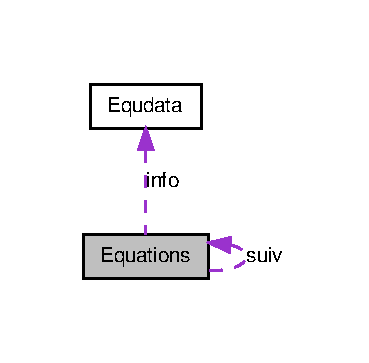
\includegraphics[width=177pt]{structEquations__coll__graph}
\end{center}
\end{figure}
\subsection*{Data Fields}
\begin{DoxyCompactItemize}
\item 
\hyperlink{equations_8h_adbcf1047b90fcdb0f3d285fb4a7c70d0}{Equtype} \hyperlink{structEquations_add825d3104abf54c01421c67536d0991}{type}
\item 
\hyperlink{unionEqudata}{Equdata} \hyperlink{structEquations_a144a9d4f5c2af07da3ecdebbeb419d66}{info}
\end{DoxyCompactItemize}


\subsection{Detailed Description}
Function pointers used for operations. 

Definition at line 68 of file equations.h.



\subsection{Field Documentation}
\hypertarget{structEquations_a144a9d4f5c2af07da3ecdebbeb419d66}{
\index{Equations@{Equations}!info@{info}}
\index{info@{info}!Equations@{Equations}}
\subsubsection[{info}]{\setlength{\rightskip}{0pt plus 5cm}{\bf Equdata} {\bf Equations::info}}}
\label{structEquations_a144a9d4f5c2af07da3ecdebbeb419d66}
Equation Data 

Definition at line 71 of file equations.h.



Referenced by Equations\_\-print().

\hypertarget{structEquations_add825d3104abf54c01421c67536d0991}{
\index{Equations@{Equations}!type@{type}}
\index{type@{type}!Equations@{Equations}}
\subsubsection[{type}]{\setlength{\rightskip}{0pt plus 5cm}{\bf Equtype} {\bf Equations::type}}}
\label{structEquations_add825d3104abf54c01421c67536d0991}
Operation constants 

Definition at line 70 of file equations.h.



Referenced by Equations\_\-print(), and Equations\_\-resultat().



The documentation for this struct was generated from the following file:\begin{DoxyCompactItemize}
\item 
metaboflux/include/\hyperlink{equations_8h}{equations.h}\end{DoxyCompactItemize}

\hypertarget{unionEqudata}{
\section{Equdata Union Reference}
\label{unionEqudata}\index{Equdata@{Equdata}}
}


Equation data.  




{\ttfamily \#include $<$equations.h$>$}

\subsection*{Data Fields}
\begin{DoxyCompactItemize}
\item 
double \hyperlink{unionEqudata_ab4b5db8558e5e8a50215854b3e8a3756}{data}
\item 
char $\ast$ \hyperlink{unionEqudata_a48bbcfc2ff891a8bcd31f90591896985}{var}
\end{DoxyCompactItemize}


\subsection{Detailed Description}
Equation data. 

Definition at line 57 of file equations.h.



\subsection{Field Documentation}
\hypertarget{unionEqudata_ab4b5db8558e5e8a50215854b3e8a3756}{
\index{Equdata@{Equdata}!data@{data}}
\index{data@{data}!Equdata@{Equdata}}
\subsubsection[{data}]{\setlength{\rightskip}{0pt plus 5cm}double {\bf Equdata::data}}}
\label{unionEqudata_ab4b5db8558e5e8a50215854b3e8a3756}
Constant 

Definition at line 60 of file equations.h.



Referenced by Equations\_\-print().

\hypertarget{unionEqudata_a48bbcfc2ff891a8bcd31f90591896985}{
\index{Equdata@{Equdata}!var@{var}}
\index{var@{var}!Equdata@{Equdata}}
\subsubsection[{var}]{\setlength{\rightskip}{0pt plus 5cm}char$\ast$ {\bf Equdata::var}}}
\label{unionEqudata_a48bbcfc2ff891a8bcd31f90591896985}
Variable 

Definition at line 61 of file equations.h.



Referenced by Equations\_\-print().



The documentation for this union was generated from the following file:\begin{DoxyCompactItemize}
\item 
metaboflux/include/\hyperlink{equations_8h}{equations.h}\end{DoxyCompactItemize}

\hypertarget{structEspeces}{
\section{Especes Struct Reference}
\label{structEspeces}\index{Especes@{Especes}}
}


Molecules data.  




{\ttfamily \#include $<$especes.h$>$}



Collaboration diagram for Especes:\nopagebreak
\begin{figure}[H]
\begin{center}
\leavevmode
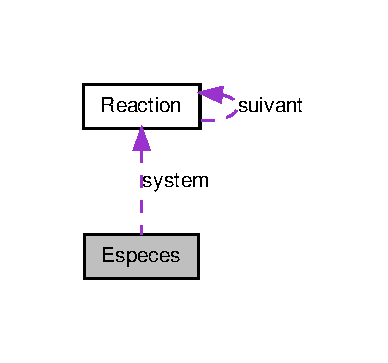
\includegraphics[width=186pt]{structEspeces__coll__graph}
\end{center}
\end{figure}
\subsection*{Data Fields}
\begin{DoxyCompactItemize}
\item 
double \hyperlink{structEspeces_ab4d42c5e3bcb897311b17030db5b882e}{quantite}
\item 
const char $\ast$ \hyperlink{structEspeces_a2fbe0a8da0e7c223e27f9bf40e48f170}{id}
\item 
\hyperlink{structReaction}{pReaction} \hyperlink{structEspeces_a61d949a99599938950d1508d7cb86d4d}{system}
\end{DoxyCompactItemize}


\subsection{Detailed Description}
Molecules data. 

Definition at line 45 of file especes.h.



\subsection{Field Documentation}
\hypertarget{structEspeces_a2fbe0a8da0e7c223e27f9bf40e48f170}{
\index{Especes@{Especes}!id@{id}}
\index{id@{id}!Especes@{Especes}}
\subsubsection[{id}]{\setlength{\rightskip}{0pt plus 5cm}const char$\ast$ {\bf Especes::id}}}
\label{structEspeces_a2fbe0a8da0e7c223e27f9bf40e48f170}
Molecule id 

Definition at line 47 of file especes.h.



Referenced by Especes\_\-save().

\hypertarget{structEspeces_ab4d42c5e3bcb897311b17030db5b882e}{
\index{Especes@{Especes}!quantite@{quantite}}
\index{quantite@{quantite}!Especes@{Especes}}
\subsubsection[{quantite}]{\setlength{\rightskip}{0pt plus 5cm}double {\bf Especes::quantite}}}
\label{structEspeces_ab4d42c5e3bcb897311b17030db5b882e}
Molecule quantity 

Definition at line 46 of file especes.h.



Referenced by Especes\_\-alloc(), Especes\_\-getQuantite(), Especes\_\-save(), Especes\_\-scoreSpecies(), and Especes\_\-setQuantite().

\hypertarget{structEspeces_a61d949a99599938950d1508d7cb86d4d}{
\index{Especes@{Especes}!system@{system}}
\index{system@{system}!Especes@{Especes}}
\subsubsection[{system}]{\setlength{\rightskip}{0pt plus 5cm}{\bf pReaction} {\bf Especes::system}}}
\label{structEspeces_a61d949a99599938950d1508d7cb86d4d}
\hyperlink{structReaction}{Reaction} where the molecule is implicated 

Definition at line 48 of file especes.h.



Referenced by Especes\_\-alloc(), Especes\_\-allocReactions(), Especes\_\-freeReactions(), Especes\_\-getNbreactions(), Especes\_\-print(), SBML\_\-EstimationReaction(), SBML\_\-reactChoice(), and SBML\_\-simulate().



The documentation for this struct was generated from the following file:\begin{DoxyCompactItemize}
\item 
metaboflux/include/\hyperlink{especes_8h}{especes.h}\end{DoxyCompactItemize}

\hypertarget{structListArguments}{
\section{ListArguments Struct Reference}
\label{structListArguments}\index{ListArguments@{ListArguments}}
}


List of arguments.  


\subsection*{Data Fields}
\begin{DoxyCompactItemize}
\item 
int \hyperlink{structListArguments_ab970afa2b3e887fdacd7cce2b24f571c}{activity}
\item 
int \hyperlink{structListArguments_a227eea65bc99120840063486d602fcbb}{debug}
\item 
int \hyperlink{structListArguments_ae2ccfbcd131374f1eab65ddc65da7468}{port}
\item 
int \hyperlink{structListArguments_a6e6b46a5655953f6a68b5cd31da094fd}{group}
\item 
char $\ast$$\ast$ \hyperlink{structListArguments_a06c7f7a5dee18ad6974749e892e01178}{files\_\-path}
\end{DoxyCompactItemize}


\subsection{Detailed Description}
List of arguments. 

Definition at line 65 of file MetaBoFlux.c.



\subsection{Field Documentation}
\hypertarget{structListArguments_ab970afa2b3e887fdacd7cce2b24f571c}{
\index{ListArguments@{ListArguments}!activity@{activity}}
\index{activity@{activity}!ListArguments@{ListArguments}}
\subsubsection[{activity}]{\setlength{\rightskip}{0pt plus 5cm}int {\bf ListArguments::activity}}}
\label{structListArguments_ab970afa2b3e887fdacd7cce2b24f571c}
Activity chosen 

Definition at line 67 of file MetaBoFlux.c.



Referenced by alloc\_\-arguments(), argument\_\-analysis(), check\_\-arguments(), and main().

\hypertarget{structListArguments_a227eea65bc99120840063486d602fcbb}{
\index{ListArguments@{ListArguments}!debug@{debug}}
\index{debug@{debug}!ListArguments@{ListArguments}}
\subsubsection[{debug}]{\setlength{\rightskip}{0pt plus 5cm}int {\bf ListArguments::debug}}}
\label{structListArguments_a227eea65bc99120840063486d602fcbb}
Debug chosen 

Definition at line 68 of file MetaBoFlux.c.



Referenced by alloc\_\-arguments(), argument\_\-analysis(), and main().

\hypertarget{structListArguments_a06c7f7a5dee18ad6974749e892e01178}{
\index{ListArguments@{ListArguments}!files\_\-path@{files\_\-path}}
\index{files\_\-path@{files\_\-path}!ListArguments@{ListArguments}}
\subsubsection[{files\_\-path}]{\setlength{\rightskip}{0pt plus 5cm}char$\ast$$\ast$ {\bf ListArguments::files\_\-path}}}
\label{structListArguments_a06c7f7a5dee18ad6974749e892e01178}
Path to files path : 0.SBML 1.PAR 2.OUT 3.RATIO\_\-FILE 4.LOG 5.OUTPUT 

Definition at line 71 of file MetaBoFlux.c.



Referenced by alloc\_\-arguments(), argument\_\-analysis(), check\_\-arguments(), check\_\-common(), free\_\-arguments(), and main().

\hypertarget{structListArguments_a6e6b46a5655953f6a68b5cd31da094fd}{
\index{ListArguments@{ListArguments}!group@{group}}
\index{group@{group}!ListArguments@{ListArguments}}
\subsubsection[{group}]{\setlength{\rightskip}{0pt plus 5cm}int {\bf ListArguments::group}}}
\label{structListArguments_a6e6b46a5655953f6a68b5cd31da094fd}
Group chosen 

Definition at line 70 of file MetaBoFlux.c.



Referenced by alloc\_\-arguments(), argument\_\-analysis(), and main().

\hypertarget{structListArguments_ae2ccfbcd131374f1eab65ddc65da7468}{
\index{ListArguments@{ListArguments}!port@{port}}
\index{port@{port}!ListArguments@{ListArguments}}
\subsubsection[{port}]{\setlength{\rightskip}{0pt plus 5cm}int {\bf ListArguments::port}}}
\label{structListArguments_ae2ccfbcd131374f1eab65ddc65da7468}
Port chosen 

Definition at line 69 of file MetaBoFlux.c.



Referenced by alloc\_\-arguments(), argument\_\-analysis(), and main().



The documentation for this struct was generated from the following file:\begin{DoxyCompactItemize}
\item 
metaboflux/src/\hyperlink{MetaBoFlux_8c}{MetaBoFlux.c}\end{DoxyCompactItemize}

\hypertarget{structListParameters}{
\section{ListParameters Struct Reference}
\label{structListParameters}\index{ListParameters@{ListParameters}}
}


Global list parameters.  




{\ttfamily \#include $<$data\_\-parameters.h$>$}



Collaboration diagram for ListParameters:\nopagebreak
\begin{figure}[H]
\begin{center}
\leavevmode
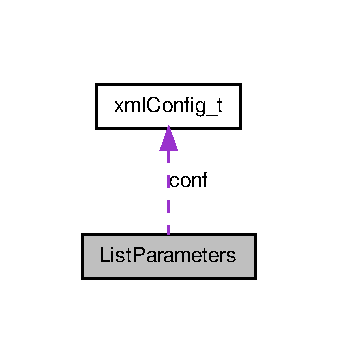
\includegraphics[width=162pt]{structListParameters__coll__graph}
\end{center}
\end{figure}
\subsection*{Data Fields}
\begin{DoxyCompactItemize}
\item 
Model\_\-t $\ast$ \hyperlink{structListParameters_ad167c56ffa16ae7c55245c7c683bbc1c}{model}
\item 
\hyperlink{structxmlConfig__t}{xmlConfig\_\-t} $\ast$ \hyperlink{structListParameters_a96adc4ee0346b24efd2139d3768be76e}{conf}
\item 
char $\ast$$\ast$$\ast$$\ast$ \hyperlink{structListParameters_a1d99e34efe708f0a4dee5f5de7a50c6c}{equation}
\item 
int \hyperlink{structListParameters_a079cdc6651256ac5ee10e546fc01ebba}{nb\_\-parameters}
\item 
int \hyperlink{structListParameters_ae9a1f821ed712556e68fe4d2d91ca1a0}{interest\_\-parameters}
\item 
int \hyperlink{structListParameters_a78464fa8003787f72be81b561fcd141a}{nb\_\-couples}
\item 
int \hyperlink{structListParameters_a45a3376021fb8e41738aa3452d7c0dbb}{nb\_\-equations}
\item 
int \hyperlink{structListParameters_a1bd4ac749f2642216552aa20a2305727}{nb\_\-reaction}
\item 
int $\ast$ \hyperlink{structListParameters_a1c994d58b286eb0b71a966c1bf079c65}{noeud}
\item 
int $\ast$ \hyperlink{structListParameters_a20e9f07e2dc0f0024591b185bd126cb0}{parameters}
\item 
char $\ast$$\ast$ \hyperlink{structListParameters_ab0d2940b00e8d0d8ae31606f79ce6373}{banned}
\item 
int \hyperlink{structListParameters_aae885063019b7630081d14786e3b48e9}{nb\_\-banned}
\item 
int \hyperlink{structListParameters_a43227ba7fdca24b48e08a561d2c417b3}{nb\_\-triesMod}
\item 
int \hyperlink{structListParameters_afb96e3b0b020bfb8d52448fac7447d3a}{nb\_\-triesSa}
\end{DoxyCompactItemize}


\subsection{Detailed Description}
Global list parameters. 

Definition at line 35 of file data\_\-parameters.h.



\subsection{Field Documentation}
\hypertarget{structListParameters_ab0d2940b00e8d0d8ae31606f79ce6373}{
\index{ListParameters@{ListParameters}!banned@{banned}}
\index{banned@{banned}!ListParameters@{ListParameters}}
\subsubsection[{banned}]{\setlength{\rightskip}{0pt plus 5cm}char$\ast$$\ast$ {\bf ListParameters::banned}}}
\label{structListParameters_ab0d2940b00e8d0d8ae31606f79ce6373}
Names of banned molecules : ex ATP, ADP ... 

Definition at line 47 of file data\_\-parameters.h.



Referenced by Data\_\-allocParameters(), Data\_\-desallocation(), Min\_\-my\_\-f(), Mod\_\-compute\_\-modeling(), Recuit\_\-energyFunction(), and Sd\_\-compute\_\-simulation().

\hypertarget{structListParameters_a96adc4ee0346b24efd2139d3768be76e}{
\index{ListParameters@{ListParameters}!conf@{conf}}
\index{conf@{conf}!ListParameters@{ListParameters}}
\subsubsection[{conf}]{\setlength{\rightskip}{0pt plus 5cm}{\bf xmlConfig\_\-t}$\ast$ {\bf ListParameters::conf}}}
\label{structListParameters_a96adc4ee0346b24efd2139d3768be76e}
Parameter file 

Definition at line 38 of file data\_\-parameters.h.



Referenced by Data\_\-allocEquations(), Data\_\-allocParameters(), Data\_\-desallocation(), Data\_\-parameters(), Data\_\-scoreAlloc(), Data\_\-simParameters(), Min\_\-my\_\-f(), Mod\_\-compute\_\-modeling(), Mpi\_\-master(), Mpi\_\-sizeResultTab(), Mpi\_\-slave(), Mpi\_\-writer(), Recuit\_\-compute\_\-recuit(), Recuit\_\-printParametre(), and Sd\_\-compute\_\-standard\_\-deviation().

\hypertarget{structListParameters_a1d99e34efe708f0a4dee5f5de7a50c6c}{
\index{ListParameters@{ListParameters}!equation@{equation}}
\index{equation@{equation}!ListParameters@{ListParameters}}
\subsubsection[{equation}]{\setlength{\rightskip}{0pt plus 5cm}char$\ast$$\ast$$\ast$$\ast$ {\bf ListParameters::equation}}}
\label{structListParameters_a1d99e34efe708f0a4dee5f5de7a50c6c}
\hyperlink{structEquations}{Equations} text 

Definition at line 39 of file data\_\-parameters.h.



Referenced by Data\_\-allocEquations(), Data\_\-desallocation(), and Data\_\-equationsInit().

\hypertarget{structListParameters_ae9a1f821ed712556e68fe4d2d91ca1a0}{
\index{ListParameters@{ListParameters}!interest\_\-parameters@{interest\_\-parameters}}
\index{interest\_\-parameters@{interest\_\-parameters}!ListParameters@{ListParameters}}
\subsubsection[{interest\_\-parameters}]{\setlength{\rightskip}{0pt plus 5cm}int {\bf ListParameters::interest\_\-parameters}}}
\label{structListParameters_ae9a1f821ed712556e68fe4d2d91ca1a0}
Number of interest parameters 

Definition at line 41 of file data\_\-parameters.h.



Referenced by Data\_\-allocParameters(), Min\_\-compute\_\-minimization(), Recuit\_\-compute\_\-recuit(), Recuit\_\-metricDistance(), Recuit\_\-printParametre(), and Recuit\_\-takeStep().

\hypertarget{structListParameters_ad167c56ffa16ae7c55245c7c683bbc1c}{
\index{ListParameters@{ListParameters}!model@{model}}
\index{model@{model}!ListParameters@{ListParameters}}
\subsubsection[{model}]{\setlength{\rightskip}{0pt plus 5cm}Model\_\-t$\ast$ {\bf ListParameters::model}}}
\label{structListParameters_ad167c56ffa16ae7c55245c7c683bbc1c}
SBML file 

Definition at line 37 of file data\_\-parameters.h.



Referenced by Data\_\-desallocation(), Data\_\-parameters(), Data\_\-scoreAlloc(), Data\_\-simParameters(), Min\_\-my\_\-f(), Mod\_\-compute\_\-modeling(), Mpi\_\-sizeResultTab(), Mpi\_\-writer(), Recuit\_\-energyFunction(), and Sd\_\-compute\_\-simulation().

\hypertarget{structListParameters_aae885063019b7630081d14786e3b48e9}{
\index{ListParameters@{ListParameters}!nb\_\-banned@{nb\_\-banned}}
\index{nb\_\-banned@{nb\_\-banned}!ListParameters@{ListParameters}}
\subsubsection[{nb\_\-banned}]{\setlength{\rightskip}{0pt plus 5cm}int {\bf ListParameters::nb\_\-banned}}}
\label{structListParameters_aae885063019b7630081d14786e3b48e9}
Number of banned molecules 

Definition at line 48 of file data\_\-parameters.h.



Referenced by Data\_\-allocParameters(), Min\_\-my\_\-f(), Mod\_\-compute\_\-modeling(), Recuit\_\-energyFunction(), and Sd\_\-compute\_\-simulation().

\hypertarget{structListParameters_a78464fa8003787f72be81b561fcd141a}{
\index{ListParameters@{ListParameters}!nb\_\-couples@{nb\_\-couples}}
\index{nb\_\-couples@{nb\_\-couples}!ListParameters@{ListParameters}}
\subsubsection[{nb\_\-couples}]{\setlength{\rightskip}{0pt plus 5cm}int {\bf ListParameters::nb\_\-couples}}}
\label{structListParameters_a78464fa8003787f72be81b561fcd141a}
Number of couples 

Definition at line 42 of file data\_\-parameters.h.



Referenced by Data\_\-allocParameters(), Data\_\-updateTab(), Min\_\-compute\_\-minimization(), Min\_\-my\_\-f(), Recuit\_\-defParametre(), and Recuit\_\-takeStep().

\hypertarget{structListParameters_a45a3376021fb8e41738aa3452d7c0dbb}{
\index{ListParameters@{ListParameters}!nb\_\-equations@{nb\_\-equations}}
\index{nb\_\-equations@{nb\_\-equations}!ListParameters@{ListParameters}}
\subsubsection[{nb\_\-equations}]{\setlength{\rightskip}{0pt plus 5cm}int {\bf ListParameters::nb\_\-equations}}}
\label{structListParameters_a45a3376021fb8e41738aa3452d7c0dbb}
Number of equations 

Definition at line 43 of file data\_\-parameters.h.



Referenced by Data\_\-allocEquations(), Data\_\-desallocation(), Data\_\-equationsAlloc(), Data\_\-equationsInit(), Min\_\-my\_\-f(), Mod\_\-compute\_\-modeling(), Recuit\_\-energyFunction(), and Sd\_\-compute\_\-simulation().

\hypertarget{structListParameters_a079cdc6651256ac5ee10e546fc01ebba}{
\index{ListParameters@{ListParameters}!nb\_\-parameters@{nb\_\-parameters}}
\index{nb\_\-parameters@{nb\_\-parameters}!ListParameters@{ListParameters}}
\subsubsection[{nb\_\-parameters}]{\setlength{\rightskip}{0pt plus 5cm}int {\bf ListParameters::nb\_\-parameters}}}
\label{structListParameters_a079cdc6651256ac5ee10e546fc01ebba}
Number of parameters 

Definition at line 40 of file data\_\-parameters.h.



Referenced by Data\_\-allocParameters(), Data\_\-allocSimParameters(), Data\_\-simParameters(), Min\_\-compute\_\-minimization(), Min\_\-getTampon(), Min\_\-my\_\-f(), Min\_\-score\_\-print\_\-mean(), Mod\_\-compute\_\-modeling(), Mod\_\-score\_\-print\_\-mean(), Mpi\_\-master(), Mpi\_\-sizeResultTab(), Mpi\_\-slave(), Mpi\_\-writeSimFile(), Recuit\_\-printPosition(), and Sd\_\-compute\_\-standard\_\-deviation().

\hypertarget{structListParameters_a1bd4ac749f2642216552aa20a2305727}{
\index{ListParameters@{ListParameters}!nb\_\-reaction@{nb\_\-reaction}}
\index{nb\_\-reaction@{nb\_\-reaction}!ListParameters@{ListParameters}}
\subsubsection[{nb\_\-reaction}]{\setlength{\rightskip}{0pt plus 5cm}int {\bf ListParameters::nb\_\-reaction}}}
\label{structListParameters_a1bd4ac749f2642216552aa20a2305727}
Number of reaction 

Definition at line 44 of file data\_\-parameters.h.

\hypertarget{structListParameters_a43227ba7fdca24b48e08a561d2c417b3}{
\index{ListParameters@{ListParameters}!nb\_\-triesMod@{nb\_\-triesMod}}
\index{nb\_\-triesMod@{nb\_\-triesMod}!ListParameters@{ListParameters}}
\subsubsection[{nb\_\-triesMod}]{\setlength{\rightskip}{0pt plus 5cm}int {\bf ListParameters::nb\_\-triesMod}}}
\label{structListParameters_a43227ba7fdca24b48e08a561d2c417b3}
Number of tries for modelling 

Definition at line 49 of file data\_\-parameters.h.



Referenced by Data\_\-allocParameters().

\hypertarget{structListParameters_afb96e3b0b020bfb8d52448fac7447d3a}{
\index{ListParameters@{ListParameters}!nb\_\-triesSa@{nb\_\-triesSa}}
\index{nb\_\-triesSa@{nb\_\-triesSa}!ListParameters@{ListParameters}}
\subsubsection[{nb\_\-triesSa}]{\setlength{\rightskip}{0pt plus 5cm}int {\bf ListParameters::nb\_\-triesSa}}}
\label{structListParameters_afb96e3b0b020bfb8d52448fac7447d3a}
Number of tries for simulated annealing and minimization 

Definition at line 50 of file data\_\-parameters.h.



Referenced by Data\_\-allocParameters(), and Recuit\_\-energyFunction().

\hypertarget{structListParameters_a1c994d58b286eb0b71a966c1bf079c65}{
\index{ListParameters@{ListParameters}!noeud@{noeud}}
\index{noeud@{noeud}!ListParameters@{ListParameters}}
\subsubsection[{noeud}]{\setlength{\rightskip}{0pt plus 5cm}int$\ast$ {\bf ListParameters::noeud}}}
\label{structListParameters_a1c994d58b286eb0b71a966c1bf079c65}
Number of nodes in an equation 

Definition at line 45 of file data\_\-parameters.h.



Referenced by Data\_\-allocEquations(), Data\_\-desallocation(), and Data\_\-equationsInit().

\hypertarget{structListParameters_a20e9f07e2dc0f0024591b185bd126cb0}{
\index{ListParameters@{ListParameters}!parameters@{parameters}}
\index{parameters@{parameters}!ListParameters@{ListParameters}}
\subsubsection[{parameters}]{\setlength{\rightskip}{0pt plus 5cm}int$\ast$ {\bf ListParameters::parameters}}}
\label{structListParameters_a20e9f07e2dc0f0024591b185bd126cb0}
Details on the parameters of reactions 

Definition at line 46 of file data\_\-parameters.h.



Referenced by Data\_\-allocParameters(), Data\_\-desallocation(), Data\_\-updateTab(), Min\_\-compute\_\-minimization(), Min\_\-my\_\-f(), Recuit\_\-defParametre(), and Recuit\_\-takeStep().



The documentation for this struct was generated from the following file:\begin{DoxyCompactItemize}
\item 
metaboflux/include/\hyperlink{data__parameters_8h}{data\_\-parameters.h}\end{DoxyCompactItemize}

\hypertarget{structoption}{
\section{option Struct Reference}
\label{structoption}\index{option@{option}}
}


List of flag for getopt.  




\subsection{Detailed Description}
List of flag for getopt. 

The documentation for this struct was generated from the following file:\begin{DoxyCompactItemize}
\item 
metaboflux/src/\hyperlink{MetaBoFlux_8c}{MetaBoFlux.c}\end{DoxyCompactItemize}

\hypertarget{structReaction}{
\section{Reaction Struct Reference}
\label{structReaction}\index{Reaction@{Reaction}}
}


Reactions data.  




{\ttfamily \#include $<$especes.h$>$}



Collaboration diagram for Reaction:\nopagebreak
\begin{figure}[H]
\begin{center}
\leavevmode
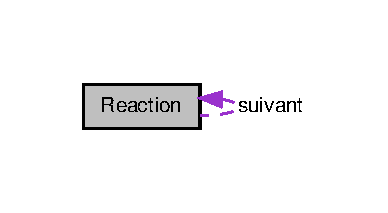
\includegraphics[width=186pt]{structReaction__coll__graph}
\end{center}
\end{figure}
\subsection*{Data Fields}
\begin{DoxyCompactItemize}
\item 
Reaction\_\-t $\ast$ \hyperlink{structReaction_ac0afd1990830008577958aec1d974e5d}{link}
\item 
struct \hyperlink{structReaction}{Reaction} $\ast$ \hyperlink{structReaction_ae0a12022d2d1cda2fe244b08a59be3d0}{suivant}
\end{DoxyCompactItemize}


\subsection{Detailed Description}
Reactions data. 

Definition at line 34 of file especes.h.



\subsection{Field Documentation}
\hypertarget{structReaction_ac0afd1990830008577958aec1d974e5d}{
\index{Reaction@{Reaction}!link@{link}}
\index{link@{link}!Reaction@{Reaction}}
\subsubsection[{link}]{\setlength{\rightskip}{0pt plus 5cm}Reaction\_\-t$\ast$ {\bf Reaction::link}}}
\label{structReaction_ac0afd1990830008577958aec1d974e5d}
\hyperlink{structReaction}{Reaction} id 

Definition at line 36 of file especes.h.



Referenced by Especes\_\-allocReactions(), Especes\_\-print(), SBML\_\-EstimationReaction(), SBML\_\-reactChoice(), and SBML\_\-simulate().

\hypertarget{structReaction_ae0a12022d2d1cda2fe244b08a59be3d0}{
\index{Reaction@{Reaction}!suivant@{suivant}}
\index{suivant@{suivant}!Reaction@{Reaction}}
\subsubsection[{suivant}]{\setlength{\rightskip}{0pt plus 5cm}struct {\bf Reaction}$\ast$ {\bf Reaction::suivant}}}
\label{structReaction_ae0a12022d2d1cda2fe244b08a59be3d0}
Next reaction implicated for the molecule 

Definition at line 38 of file especes.h.



Referenced by Especes\_\-allocReactions(), Especes\_\-freeReactions(), Especes\_\-getNbreactions(), Especes\_\-print(), SBML\_\-EstimationReaction(), and SBML\_\-reactChoice().



The documentation for this struct was generated from the following file:\begin{DoxyCompactItemize}
\item 
metaboflux/include/\hyperlink{especes_8h}{especes.h}\end{DoxyCompactItemize}

\hypertarget{structScore}{
\section{Score Struct Reference}
\label{structScore}\index{Score@{Score}}
}


Structure containing all information from simulations.  




{\ttfamily \#include $<$simulation.h$>$}

\subsection*{Data Fields}
\begin{DoxyCompactItemize}
\item 
char $\ast$$\ast$ \hyperlink{structScore_a29547e98673d89a8964a747015b2c26c}{name}
\item 
double $\ast$ \hyperlink{structScore_aadd3a70f5dc0018739a48ff13cb9fa2d}{quantite}
\item 
char $\ast$$\ast$ \hyperlink{structScore_af8245823c6e659cee49999dd3452a301}{reaction}
\item 
int \hyperlink{structScore_a9676111bf63c8d420921fe1c9187670d}{nb\_\-reaction}
\item 
int \hyperlink{structScore_a103843cc09238d77051b5a6ca4e48173}{tailleReactions}
\item 
int \hyperlink{structScore_ac5a5af5f70e341fb42ea765394d86207}{tailleSpecies}
\item 
int \hyperlink{structScore_aee1e19fc90d330de6fced582dff7102c}{taille}
\item 
char $\ast$$\ast$ \hyperlink{structScore_ae22017a9e14dbbacbc7ef1a41f880ceb}{species}
\item 
int \hyperlink{structScore_a88d07328145c2565fb2fa50c31760dbe}{nb\_\-species}
\item 
int $\ast$ \hyperlink{structScore_abb78b9e380ec83ab8f0274480c420be7}{species\_\-amount}
\item 
int $\ast$ \hyperlink{structScore_a46e74b92b29101ec9dc68255ab71a480}{species\_\-weight}
\end{DoxyCompactItemize}


\subsection{Detailed Description}
Structure containing all information from simulations. 

Definition at line 51 of file simulation.h.



\subsection{Field Documentation}
\hypertarget{structScore_a29547e98673d89a8964a747015b2c26c}{
\index{Score@{Score}!name@{name}}
\index{name@{name}!Score@{Score}}
\subsubsection[{name}]{\setlength{\rightskip}{0pt plus 5cm}char$\ast$$\ast$ {\bf Score::name}}}
\label{structScore_a29547e98673d89a8964a747015b2c26c}
Molecules id 

Definition at line 53 of file simulation.h.



Referenced by Data\_\-allocScore(), Data\_\-desallocSim(), Data\_\-scoreFree(), Min\_\-my\_\-f(), Min\_\-score\_\-print\_\-mean(), Mod\_\-compute\_\-modeling(), Mod\_\-score\_\-print\_\-mean(), Recuit\_\-energyFunction(), SBML\_\-score(), SBML\_\-score\_\-add(), and Sd\_\-compute\_\-simulation().

\hypertarget{structScore_a9676111bf63c8d420921fe1c9187670d}{
\index{Score@{Score}!nb\_\-reaction@{nb\_\-reaction}}
\index{nb\_\-reaction@{nb\_\-reaction}!Score@{Score}}
\subsubsection[{nb\_\-reaction}]{\setlength{\rightskip}{0pt plus 5cm}int {\bf Score::nb\_\-reaction}}}
\label{structScore_a9676111bf63c8d420921fe1c9187670d}
Number of reaction 

Definition at line 56 of file simulation.h.



Referenced by Data\_\-allocScore(), Data\_\-desallocSim(), Data\_\-scoreFree(), SBML\_\-score(), and SBML\_\-setReactions().

\hypertarget{structScore_a88d07328145c2565fb2fa50c31760dbe}{
\index{Score@{Score}!nb\_\-species@{nb\_\-species}}
\index{nb\_\-species@{nb\_\-species}!Score@{Score}}
\subsubsection[{nb\_\-species}]{\setlength{\rightskip}{0pt plus 5cm}int {\bf Score::nb\_\-species}}}
\label{structScore_a88d07328145c2565fb2fa50c31760dbe}
Number of molecules 

Definition at line 61 of file simulation.h.



Referenced by Data\_\-allocScore(), Min\_\-my\_\-f(), Min\_\-score\_\-print\_\-mean(), Mod\_\-compute\_\-modeling(), Mod\_\-score\_\-print\_\-mean(), Recuit\_\-energyFunction(), and Sd\_\-compute\_\-simulation().

\hypertarget{structScore_aadd3a70f5dc0018739a48ff13cb9fa2d}{
\index{Score@{Score}!quantite@{quantite}}
\index{quantite@{quantite}!Score@{Score}}
\subsubsection[{quantite}]{\setlength{\rightskip}{0pt plus 5cm}double$\ast$ {\bf Score::quantite}}}
\label{structScore_aadd3a70f5dc0018739a48ff13cb9fa2d}
Quantity of molecules 

Definition at line 54 of file simulation.h.



Referenced by Data\_\-allocScore(), Data\_\-desallocSim(), Data\_\-scoreFree(), Data\_\-scoreInit(), Min\_\-getTampon(), Min\_\-my\_\-f(), Min\_\-score\_\-print\_\-mean(), Mod\_\-compute\_\-modeling(), Mod\_\-score\_\-print\_\-mean(), Recuit\_\-energyFunction(), SBML\_\-score(), SBML\_\-score\_\-add(), SBML\_\-score\_\-mean(), and Sd\_\-compute\_\-simulation().

\hypertarget{structScore_af8245823c6e659cee49999dd3452a301}{
\index{Score@{Score}!reaction@{reaction}}
\index{reaction@{reaction}!Score@{Score}}
\subsubsection[{reaction}]{\setlength{\rightskip}{0pt plus 5cm}char$\ast$$\ast$ {\bf Score::reaction}}}
\label{structScore_af8245823c6e659cee49999dd3452a301}
Interest reaction 

Definition at line 55 of file simulation.h.



Referenced by Data\_\-allocScore(), Data\_\-desallocSim(), Data\_\-scoreFree(), SBML\_\-score(), and SBML\_\-setReactions().

\hypertarget{structScore_ae22017a9e14dbbacbc7ef1a41f880ceb}{
\index{Score@{Score}!species@{species}}
\index{species@{species}!Score@{Score}}
\subsubsection[{species}]{\setlength{\rightskip}{0pt plus 5cm}char$\ast$$\ast$ {\bf Score::species}}}
\label{structScore_ae22017a9e14dbbacbc7ef1a41f880ceb}
Interest molecules 

Definition at line 60 of file simulation.h.



Referenced by Data\_\-allocScore(), Data\_\-desallocSim(), Min\_\-my\_\-f(), Min\_\-score\_\-print\_\-mean(), Mod\_\-compute\_\-modeling(), Mod\_\-score\_\-print\_\-mean(), Recuit\_\-energyFunction(), and Sd\_\-compute\_\-simulation().

\hypertarget{structScore_abb78b9e380ec83ab8f0274480c420be7}{
\index{Score@{Score}!species\_\-amount@{species\_\-amount}}
\index{species\_\-amount@{species\_\-amount}!Score@{Score}}
\subsubsection[{species\_\-amount}]{\setlength{\rightskip}{0pt plus 5cm}int$\ast$ {\bf Score::species\_\-amount}}}
\label{structScore_abb78b9e380ec83ab8f0274480c420be7}
Quantity of the interest molecules 

Definition at line 62 of file simulation.h.



Referenced by Data\_\-allocScore(), Data\_\-desallocSim(), Data\_\-scoreFree(), Min\_\-my\_\-f(), Min\_\-score\_\-print\_\-mean(), Mod\_\-compute\_\-modeling(), Mod\_\-score\_\-print\_\-mean(), Recuit\_\-energyFunction(), and Sd\_\-compute\_\-simulation().

\hypertarget{structScore_a46e74b92b29101ec9dc68255ab71a480}{
\index{Score@{Score}!species\_\-weight@{species\_\-weight}}
\index{species\_\-weight@{species\_\-weight}!Score@{Score}}
\subsubsection[{species\_\-weight}]{\setlength{\rightskip}{0pt plus 5cm}int$\ast$ {\bf Score::species\_\-weight}}}
\label{structScore_a46e74b92b29101ec9dc68255ab71a480}
Weight of the interest molecules 

Definition at line 63 of file simulation.h.



Referenced by Data\_\-allocScore(), Data\_\-desallocSim(), Data\_\-scoreFree(), Min\_\-my\_\-f(), Mod\_\-compute\_\-modeling(), Recuit\_\-energyFunction(), and Sd\_\-compute\_\-simulation().

\hypertarget{structScore_aee1e19fc90d330de6fced582dff7102c}{
\index{Score@{Score}!taille@{taille}}
\index{taille@{taille}!Score@{Score}}
\subsubsection[{taille}]{\setlength{\rightskip}{0pt plus 5cm}int {\bf Score::taille}}}
\label{structScore_aee1e19fc90d330de6fced582dff7102c}
Total of other two sizes 

Definition at line 59 of file simulation.h.



Referenced by Data\_\-allocScore(), Data\_\-desallocSim(), Data\_\-scoreFree(), Data\_\-scoreInit(), Min\_\-getTampon(), Min\_\-my\_\-f(), Min\_\-score\_\-print\_\-mean(), Mod\_\-compute\_\-modeling(), Mod\_\-score\_\-print\_\-mean(), Recuit\_\-energyFunction(), SBML\_\-score\_\-add(), SBML\_\-score\_\-mean(), and Sd\_\-compute\_\-simulation().

\hypertarget{structScore_a103843cc09238d77051b5a6ca4e48173}{
\index{Score@{Score}!tailleReactions@{tailleReactions}}
\index{tailleReactions@{tailleReactions}!Score@{Score}}
\subsubsection[{tailleReactions}]{\setlength{\rightskip}{0pt plus 5cm}int {\bf Score::tailleReactions}}}
\label{structScore_a103843cc09238d77051b5a6ca4e48173}
Number of reaction in the SBML file 

Definition at line 57 of file simulation.h.



Referenced by Data\_\-allocScore(), and SBML\_\-compute\_\-simulation().

\hypertarget{structScore_ac5a5af5f70e341fb42ea765394d86207}{
\index{Score@{Score}!tailleSpecies@{tailleSpecies}}
\index{tailleSpecies@{tailleSpecies}!Score@{Score}}
\subsubsection[{tailleSpecies}]{\setlength{\rightskip}{0pt plus 5cm}int {\bf Score::tailleSpecies}}}
\label{structScore_ac5a5af5f70e341fb42ea765394d86207}
Number of molecules in the SBML file 

Definition at line 58 of file simulation.h.



Referenced by Data\_\-allocScore(), Min\_\-my\_\-f(), Min\_\-score\_\-print\_\-mean(), Mod\_\-compute\_\-modeling(), Mod\_\-score\_\-print\_\-mean(), Recuit\_\-energyFunction(), SBML\_\-compute\_\-simulation(), SBML\_\-score\_\-add(), and Sd\_\-compute\_\-simulation().



The documentation for this struct was generated from the following file:\begin{DoxyCompactItemize}
\item 
metaboflux/include/\hyperlink{simulation_8h}{simulation.h}\end{DoxyCompactItemize}

\hypertarget{structSimParameters}{
\section{SimParameters Struct Reference}
\label{structSimParameters}\index{SimParameters@{SimParameters}}
}


List of parameters specific to each simulation.  




{\ttfamily \#include $<$data\_\-parameters.h$>$}



Collaboration diagram for SimParameters:\nopagebreak
\begin{figure}[H]
\begin{center}
\leavevmode
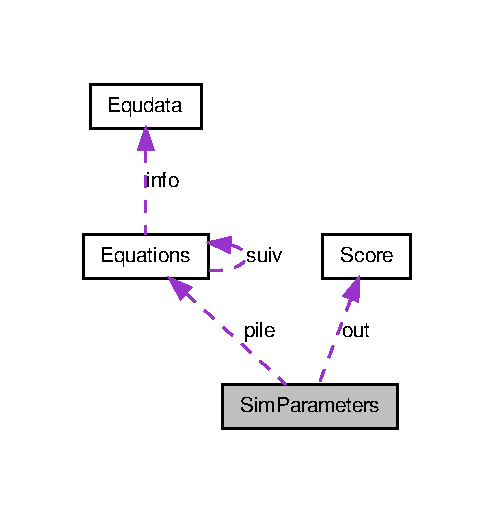
\includegraphics[width=237pt]{structSimParameters__coll__graph}
\end{center}
\end{figure}
\subsection*{Data Fields}
\begin{DoxyCompactItemize}
\item 
\hyperlink{structEquations}{Equations} $\ast$$\ast$ \hyperlink{structSimParameters_aecbff20f6647d4d348d3026e166a5c93}{pile}
\item 
\hyperlink{structScore}{pScore} \hyperlink{structSimParameters_a0dc198d74946f531dbf36860796bf108}{out}
\item 
gsl\_\-rng $\ast$ \hyperlink{structSimParameters_a3657bf540ffac966ca5e6e48595370ac}{r}
\item 
double $\ast$ \hyperlink{structSimParameters_aba46fa332475a2c74856712fa0ca10a0}{y}
\item 
FILE $\ast$ \hyperlink{structSimParameters_aad7fb1c37993627a2c2c04b7509ce3c0}{debugFile}
\end{DoxyCompactItemize}


\subsection{Detailed Description}
List of parameters specific to each simulation. 

Definition at line 58 of file data\_\-parameters.h.



\subsection{Field Documentation}
\hypertarget{structSimParameters_aad7fb1c37993627a2c2c04b7509ce3c0}{
\index{SimParameters@{SimParameters}!debugFile@{debugFile}}
\index{debugFile@{debugFile}!SimParameters@{SimParameters}}
\subsubsection[{debugFile}]{\setlength{\rightskip}{0pt plus 5cm}FILE$\ast$ {\bf SimParameters::debugFile}}}
\label{structSimParameters_aad7fb1c37993627a2c2c04b7509ce3c0}
Debug file : storage of intermediate values of the simulations 

Definition at line 64 of file data\_\-parameters.h.



Referenced by Data\_\-desallocSim(), Data\_\-simParameters(), Min\_\-my\_\-f(), Mod\_\-compute\_\-modeling(), Recuit\_\-energyFunction(), and Sd\_\-compute\_\-simulation().

\hypertarget{structSimParameters_a0dc198d74946f531dbf36860796bf108}{
\index{SimParameters@{SimParameters}!out@{out}}
\index{out@{out}!SimParameters@{SimParameters}}
\subsubsection[{out}]{\setlength{\rightskip}{0pt plus 5cm}{\bf pScore} {\bf SimParameters::out}}}
\label{structSimParameters_a0dc198d74946f531dbf36860796bf108}
\hyperlink{structScore}{Score} 

Definition at line 61 of file data\_\-parameters.h.



Referenced by Data\_\-desallocSim(), Data\_\-simParameters(), Min\_\-getTampon(), Min\_\-my\_\-f(), Min\_\-score\_\-print\_\-mean(), Mod\_\-compute\_\-modeling(), Mod\_\-score\_\-print\_\-mean(), Recuit\_\-energyFunction(), and Sd\_\-compute\_\-simulation().

\hypertarget{structSimParameters_aecbff20f6647d4d348d3026e166a5c93}{
\index{SimParameters@{SimParameters}!pile@{pile}}
\index{pile@{pile}!SimParameters@{SimParameters}}
\subsubsection[{pile}]{\setlength{\rightskip}{0pt plus 5cm}{\bf Equations}$\ast$$\ast$ {\bf SimParameters::pile}}}
\label{structSimParameters_aecbff20f6647d4d348d3026e166a5c93}
Interpreted \hyperlink{structEquations}{Equations} 

Definition at line 60 of file data\_\-parameters.h.



Referenced by Data\_\-simParameters(), Min\_\-my\_\-f(), Mod\_\-compute\_\-modeling(), Recuit\_\-energyFunction(), and Sd\_\-compute\_\-simulation().

\hypertarget{structSimParameters_a3657bf540ffac966ca5e6e48595370ac}{
\index{SimParameters@{SimParameters}!r@{r}}
\index{r@{r}!SimParameters@{SimParameters}}
\subsubsection[{r}]{\setlength{\rightskip}{0pt plus 5cm}gsl\_\-rng$\ast$ {\bf SimParameters::r}}}
\label{structSimParameters_a3657bf540ffac966ca5e6e48595370ac}
Random number generator 

Definition at line 62 of file data\_\-parameters.h.



Referenced by Data\_\-desallocSim(), Data\_\-simParameters(), Min\_\-my\_\-f(), Mod\_\-compute\_\-modeling(), Recuit\_\-compute\_\-recuit(), Recuit\_\-energyFunction(), and Sd\_\-compute\_\-simulation().

\hypertarget{structSimParameters_aba46fa332475a2c74856712fa0ca10a0}{
\index{SimParameters@{SimParameters}!y@{y}}
\index{y@{y}!SimParameters@{SimParameters}}
\subsubsection[{y}]{\setlength{\rightskip}{0pt plus 5cm}double$\ast$ {\bf SimParameters::y}}}
\label{structSimParameters_aba46fa332475a2c74856712fa0ca10a0}
Table of reaction parameters 

Definition at line 63 of file data\_\-parameters.h.



Referenced by Data\_\-copieTab(), Data\_\-desallocSim(), Data\_\-simParameters(), Min\_\-compute\_\-minimization(), Min\_\-copieTab2(), Min\_\-copieTab3(), Min\_\-getTampon(), Min\_\-my\_\-f(), Min\_\-score\_\-print\_\-mean(), Mod\_\-compute\_\-modeling(), Mod\_\-score\_\-print\_\-mean(), Recuit\_\-energyFunction(), Recuit\_\-printPosition(), Sd\_\-compute\_\-simulation(), and Sd\_\-compute\_\-standard\_\-deviation().



The documentation for this struct was generated from the following file:\begin{DoxyCompactItemize}
\item 
metaboflux/include/\hyperlink{data__parameters_8h}{data\_\-parameters.h}\end{DoxyCompactItemize}

\hypertarget{structTestReaction}{
\section{TestReaction Struct Reference}
\label{structTestReaction}\index{TestReaction@{TestReaction}}
}


Structure used to test reactions.  




{\ttfamily \#include $<$simulation.h$>$}

\subsection*{Data Fields}
\begin{DoxyCompactItemize}
\item 
Reaction\_\-t $\ast$$\ast$ \hyperlink{structTestReaction_abc440bf3f3edc3d4ca6ad896962ffad2}{tabReactions}
\item 
int $\ast$ \hyperlink{structTestReaction_a04037c90652dceaab2f416e099be460c}{minStepTab}
\end{DoxyCompactItemize}


\subsection{Detailed Description}
Structure used to test reactions. 

Definition at line 40 of file simulation.h.



\subsection{Field Documentation}
\hypertarget{structTestReaction_a04037c90652dceaab2f416e099be460c}{
\index{TestReaction@{TestReaction}!minStepTab@{minStepTab}}
\index{minStepTab@{minStepTab}!TestReaction@{TestReaction}}
\subsubsection[{minStepTab}]{\setlength{\rightskip}{0pt plus 5cm}int$\ast$ {\bf TestReaction::minStepTab}}}
\label{structTestReaction_a04037c90652dceaab2f416e099be460c}
Stock le nombre de realisation possible pour cette reaction 

Definition at line 43 of file simulation.h.



Referenced by SBML\_\-allocTest(), SBML\_\-EstimationReaction(), and SBML\_\-freeTest().

\hypertarget{structTestReaction_abc440bf3f3edc3d4ca6ad896962ffad2}{
\index{TestReaction@{TestReaction}!tabReactions@{tabReactions}}
\index{tabReactions@{tabReactions}!TestReaction@{TestReaction}}
\subsubsection[{tabReactions}]{\setlength{\rightskip}{0pt plus 5cm}Reaction\_\-t$\ast$$\ast$ {\bf TestReaction::tabReactions}}}
\label{structTestReaction_abc440bf3f3edc3d4ca6ad896962ffad2}
Stock temporairement une reaction 

Definition at line 42 of file simulation.h.



Referenced by SBML\_\-allocTest(), SBML\_\-EstimationReaction(), and SBML\_\-freeTest().



The documentation for this struct was generated from the following file:\begin{DoxyCompactItemize}
\item 
metaboflux/include/\hyperlink{simulation_8h}{simulation.h}\end{DoxyCompactItemize}

\hypertarget{structxmlConfig__t}{
\section{xmlConfig\_\-t Struct Reference}
\label{structxmlConfig__t}\index{xmlConfig\_\-t@{xmlConfig\_\-t}}
}


Structure containing all information from parameter.xml.  




{\ttfamily \#include $<$xml\_\-parameter.h$>$}

\subsection*{Data Fields}
\begin{DoxyCompactItemize}
\item 
char $\ast$ \hyperlink{structxmlConfig__t_a7a2f1cbf9d3b49f1b2debb85a8606658}{fichier}
\item 
xmlDocPtr \hyperlink{structxmlConfig__t_a35e7e8fc3398d0866fbf91b0245fd7b9}{doc}
\item 
xmlNodePtr \hyperlink{structxmlConfig__t_a535cd8a3e33d4ae2a00ab29f32a442ff}{racine}
\item 
xmlXPathContextPtr \hyperlink{structxmlConfig__t_ae21311533cb59c9752bf21ffce5d5316}{ctxt}
\end{DoxyCompactItemize}


\subsection{Detailed Description}
Structure containing all information from parameter.xml. 

Definition at line 33 of file xml\_\-parameter.h.



\subsection{Field Documentation}
\hypertarget{structxmlConfig__t_ae21311533cb59c9752bf21ffce5d5316}{
\index{xmlConfig\_\-t@{xmlConfig\_\-t}!ctxt@{ctxt}}
\index{ctxt@{ctxt}!xmlConfig_t@{xmlConfig\_\-t}}
\subsubsection[{ctxt}]{\setlength{\rightskip}{0pt plus 5cm}xmlXPathContextPtr {\bf xmlConfig\_\-t::ctxt}}}
\label{structxmlConfig__t_ae21311533cb59c9752bf21ffce5d5316}
Xml ctxt 

Definition at line 37 of file xml\_\-parameter.h.



Referenced by Xml\_\-freeConfig(), Xml\_\-getBanned(), Xml\_\-getCount(), Xml\_\-getDoubleNumber(), Xml\_\-getKineticLaw(), Xml\_\-getKineticLawNodes(), Xml\_\-getNumber(), Xml\_\-getReactionsNames(), Xml\_\-getReactionsNamesinNoeud(), Xml\_\-getSpeciesFinalAmount(), Xml\_\-getSpeciesWeight(), Xml\_\-getString(), and Xml\_\-loadConfig().

\hypertarget{structxmlConfig__t_a35e7e8fc3398d0866fbf91b0245fd7b9}{
\index{xmlConfig\_\-t@{xmlConfig\_\-t}!doc@{doc}}
\index{doc@{doc}!xmlConfig_t@{xmlConfig\_\-t}}
\subsubsection[{doc}]{\setlength{\rightskip}{0pt plus 5cm}xmlDocPtr {\bf xmlConfig\_\-t::doc}}}
\label{structxmlConfig__t_a35e7e8fc3398d0866fbf91b0245fd7b9}
Xml doc 

Definition at line 35 of file xml\_\-parameter.h.



Referenced by Xml\_\-freeConfig(), and Xml\_\-loadConfig().

\hypertarget{structxmlConfig__t_a7a2f1cbf9d3b49f1b2debb85a8606658}{
\index{xmlConfig\_\-t@{xmlConfig\_\-t}!fichier@{fichier}}
\index{fichier@{fichier}!xmlConfig_t@{xmlConfig\_\-t}}
\subsubsection[{fichier}]{\setlength{\rightskip}{0pt plus 5cm}char$\ast$ {\bf xmlConfig\_\-t::fichier}}}
\label{structxmlConfig__t_a7a2f1cbf9d3b49f1b2debb85a8606658}
Name of the parameter file 

Definition at line 34 of file xml\_\-parameter.h.



Referenced by Xml\_\-freeConfig(), and Xml\_\-loadConfig().

\hypertarget{structxmlConfig__t_a535cd8a3e33d4ae2a00ab29f32a442ff}{
\index{xmlConfig\_\-t@{xmlConfig\_\-t}!racine@{racine}}
\index{racine@{racine}!xmlConfig_t@{xmlConfig\_\-t}}
\subsubsection[{racine}]{\setlength{\rightskip}{0pt plus 5cm}xmlNodePtr {\bf xmlConfig\_\-t::racine}}}
\label{structxmlConfig__t_a535cd8a3e33d4ae2a00ab29f32a442ff}
Xml root 

Definition at line 36 of file xml\_\-parameter.h.



Referenced by Xml\_\-loadConfig().



The documentation for this struct was generated from the following file:\begin{DoxyCompactItemize}
\item 
metaboflux/include/\hyperlink{xml__parameter_8h}{xml\_\-parameter.h}\end{DoxyCompactItemize}

\chapter{File Documentation}
\hypertarget{data__parameters_8h}{
\section{metaboflux/include/data\_\-parameters.h File Reference}
\label{data__parameters_8h}\index{metaboflux/include/data\_\-parameters.h@{metaboflux/include/data\_\-parameters.h}}
}


Load data parameters.  


This graph shows which files directly or indirectly include this file:\nopagebreak
\begin{figure}[H]
\begin{center}
\leavevmode
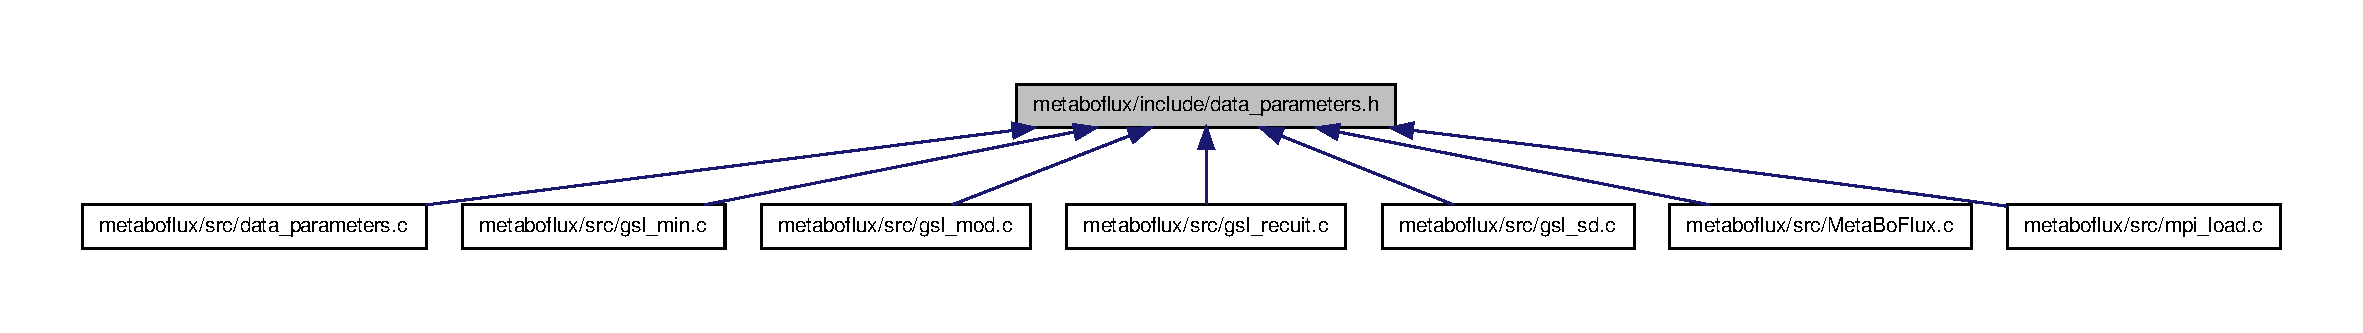
\includegraphics[width=400pt]{data__parameters_8h__dep__incl}
\end{center}
\end{figure}
\subsection*{Data Structures}
\begin{DoxyCompactItemize}
\item 
struct \hyperlink{structListParameters}{ListParameters}
\begin{DoxyCompactList}\small\item\em Global list parameters. \end{DoxyCompactList}\item 
struct \hyperlink{structSimParameters}{SimParameters}
\begin{DoxyCompactList}\small\item\em List of parameters specific to each simulation. \end{DoxyCompactList}\end{DoxyCompactItemize}
\subsection*{Functions}
\begin{DoxyCompactItemize}
\item 
\hyperlink{structxmlConfig__t}{xmlConfig\_\-t} $\ast$ \hyperlink{data__parameters_8h_a6de2ffa5b44477da0d4a2e9e831c0c8a}{Data\_\-initXML} (char $\ast$)
\begin{DoxyCompactList}\small\item\em Load parameter file. \end{DoxyCompactList}\item 
Model\_\-t $\ast$ \hyperlink{data__parameters_8h_a2c7c500f91d49ea904f26078df0c0410}{Data\_\-initSBML} (char $\ast$)
\begin{DoxyCompactList}\small\item\em Load SBML file. \end{DoxyCompactList}\item 
gsl\_\-rng $\ast$ \hyperlink{data__parameters_8h_a82ec4869c2eb338089f664171740b07b}{Data\_\-rngAlloc} (gsl\_\-rng $\ast$)
\begin{DoxyCompactList}\small\item\em Allocation of the random number generator. \end{DoxyCompactList}\item 
\hyperlink{structEquations}{Equations} $\ast$$\ast$ \hyperlink{data__parameters_8h_a0940064d850a6ea789bb94e0fd635d0d}{Data\_\-equationsAlloc} (\hyperlink{structListParameters}{pListParameters}, \hyperlink{structEquations}{Equations} $\ast$$\ast$)
\begin{DoxyCompactList}\small\item\em Allocate the struct \hyperlink{structEquations}{Equations}. \end{DoxyCompactList}\item 
void \hyperlink{data__parameters_8h_ac0ac001f1fc3102e3ed07568cba5c570}{Data\_\-equationsInit} (\hyperlink{structListParameters}{pListParameters}, \hyperlink{structEquations}{Equations} $\ast$$\ast$)
\begin{DoxyCompactList}\small\item\em Initialize equations. \end{DoxyCompactList}\item 
void \hyperlink{data__parameters_8h_a014a6fdcabd0d2dbfee53acf4a32e218}{Data\_\-allocEquations} (\hyperlink{structListParameters}{pListParameters} a)
\begin{DoxyCompactList}\small\item\em Allocate the different elements related to he struct \hyperlink{structEquations}{Equations}. \end{DoxyCompactList}\item 
void \hyperlink{data__parameters_8h_a46e8fbe37a14a679690ad84c4a596cc4}{Data\_\-allocScore} (\hyperlink{structScore}{pScore}, \hyperlink{structxmlConfig__t}{xmlConfig\_\-t} $\ast$, Model\_\-t $\ast$)
\begin{DoxyCompactList}\small\item\em Copy the partial table x in the full table y. \end{DoxyCompactList}\item 
\hyperlink{structScore}{pScore} \hyperlink{data__parameters_8h_a28bd10646fcc4410a1d1d6433e84ea95}{Data\_\-scoreAlloc} (\hyperlink{structListParameters}{pListParameters})
\begin{DoxyCompactList}\small\item\em Allocation of the struct \hyperlink{structScore}{Score}. \end{DoxyCompactList}\item 
void \hyperlink{data__parameters_8h_a9096849f5a525ee26634b2d98a497ded}{Data\_\-scoreInit} (\hyperlink{structScore}{pScore})
\begin{DoxyCompactList}\small\item\em Initialize the struct \hyperlink{structScore}{Score}. \end{DoxyCompactList}\item 
void \hyperlink{data__parameters_8h_af65c1571388a7669aaa18c4163dac2f1}{Data\_\-scoreFree} (\hyperlink{structScore}{pScore})
\begin{DoxyCompactList}\small\item\em Free the struct \hyperlink{structScore}{Score}. \end{DoxyCompactList}\item 
int \hyperlink{data__parameters_8h_a27598d9ebdecd23858dc015d34daa9f8}{Data\_\-copieTab} (\hyperlink{structSimParameters}{pSimParameters}, double $\ast$, int, int, int)
\begin{DoxyCompactList}\small\item\em Copy the partial table x in the full table y. \end{DoxyCompactList}\item 
void \hyperlink{data__parameters_8h_aedfc4262f7adadcd89741626ddcf0eef}{Data\_\-updateTab} (\hyperlink{structListParameters}{pListParameters}, \hyperlink{structSimParameters}{pSimParameters}, double $\ast$)
\begin{DoxyCompactList}\small\item\em Copy table. \end{DoxyCompactList}\item 
void \hyperlink{data__parameters_8h_a7f131c19d7d1bc29db5ccf53b0517fdf}{Data\_\-allocSimParameters} (double $\ast$, \hyperlink{structListParameters}{pListParameters})
\begin{DoxyCompactList}\small\item\em Allocation of tables needed for simulations. \end{DoxyCompactList}\item 
void \hyperlink{data__parameters_8h_ada6a0c0e47ea4e678bbd615c9371e8af}{Data\_\-allocParameters} (\hyperlink{structListParameters}{pListParameters})
\begin{DoxyCompactList}\small\item\em Copy the partial table x in the full table y. \end{DoxyCompactList}\item 
void \hyperlink{data__parameters_8h_a9cfc3bfbb7f489152efcbfa77e23bcf6}{Data\_\-parameters} (\hyperlink{structListParameters}{pListParameters}, char $\ast$$\ast$)
\begin{DoxyCompactList}\small\item\em Record parameters of the simulation. \end{DoxyCompactList}\item 
void \hyperlink{data__parameters_8h_ab08889cc0af85b8a2e8938972107d645}{Data\_\-desallocation} (\hyperlink{structListParameters}{pListParameters})
\begin{DoxyCompactList}\small\item\em Free memory allocated to the various objects of the program. \end{DoxyCompactList}\item 
void \hyperlink{data__parameters_8h_a2f0df5c0de22994cb0aec62dba0e1bd5}{Data\_\-simParameters} (\hyperlink{structListParameters}{pListParameters}, \hyperlink{structSimParameters}{pSimParameters}, char $\ast$, char $\ast$, int, int)
\begin{DoxyCompactList}\small\item\em Recording parameters specific to each simulation. \end{DoxyCompactList}\item 
void \hyperlink{data__parameters_8h_a77e81e9bc2cd1ffe83bb3b8b2ecc4454}{Data\_\-desallocSim} (\hyperlink{structSimParameters}{pSimParameters})
\begin{DoxyCompactList}\small\item\em Free struct parameters specific to each simulation. \end{DoxyCompactList}\end{DoxyCompactItemize}


\subsection{Detailed Description}
Load data parameters. This file is part of MetaBoFlux (\href{http://www.cbib.u-bordeaux2.fr/metaboflux/}{\tt http://www.cbib.u-\/bordeaux2.fr/metaboflux/}) Copyright (C) 2010 Amine Ghozlane from LaBRI and University of Bordeaux 1

MetaBoFlux is free software: you can redistribute it and/or modify it under the terms of the GNU Lesser General Public License as published by the Free Software Foundation, either version 3 of the License, or (at your option) any later version.

MetaBoFlux is distributed in the hope that it will be useful, but WITHOUT ANY WARRANTY; without even the implied warranty of MERCHANTABILITY or FITNESS FOR A PARTICULAR PURPOSE. See the GNU General Public License for more details.

You should have received a copy of the GNU Lesser General Public License along with this program. If not, see $<$\href{http://www.gnu.org/licenses/}{\tt http://www.gnu.org/licenses/}$>$.

\begin{DoxyAuthor}{Author}
\{Amine Ghozlane\} 
\end{DoxyAuthor}
\begin{DoxyVersion}{Version}
2.0 
\end{DoxyVersion}
\begin{DoxyDate}{Date}
10 novembre 2010 
\end{DoxyDate}


Definition in file \hyperlink{data__parameters_8h_source}{data\_\-parameters.h}.



\subsection{Function Documentation}
\hypertarget{data__parameters_8h_a014a6fdcabd0d2dbfee53acf4a32e218}{
\index{data\_\-parameters.h@{data\_\-parameters.h}!Data\_\-allocEquations@{Data\_\-allocEquations}}
\index{Data\_\-allocEquations@{Data\_\-allocEquations}!data_parameters.h@{data\_\-parameters.h}}
\subsubsection[{Data\_\-allocEquations}]{\setlength{\rightskip}{0pt plus 5cm}void Data\_\-allocEquations (
\begin{DoxyParamCaption}
\item[{{\bf pListParameters}}]{a}
\end{DoxyParamCaption}
)}}
\label{data__parameters_8h_a014a6fdcabd0d2dbfee53acf4a32e218}


Allocate the different elements related to he struct \hyperlink{structEquations}{Equations}. 

\begin{DoxyAuthor}{Author}
Amine Ghozlane 
\end{DoxyAuthor}

\begin{DoxyParams}{Parameters}
{\em a} & Global parameters : struct \hyperlink{structListParameters}{ListParameters} \\
\hline
\end{DoxyParams}


Definition at line 202 of file data\_\-parameters.c.



References ListParameters::conf, ListParameters::equation, ListParameters::nb\_\-equations, ListParameters::noeud, Xml\_\-getKineticLaw(), Xml\_\-getKineticLawNodes(), and Xml\_\-getNbEquations().



Referenced by Data\_\-parameters().



Here is the call graph for this function:\nopagebreak
\begin{figure}[H]
\begin{center}
\leavevmode
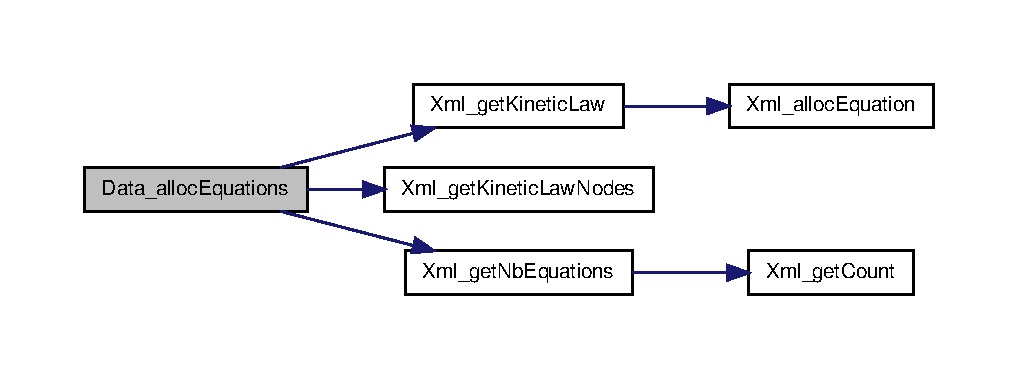
\includegraphics[width=400pt]{data__parameters_8h_a014a6fdcabd0d2dbfee53acf4a32e218_cgraph}
\end{center}
\end{figure}


\hypertarget{data__parameters_8h_ada6a0c0e47ea4e678bbd615c9371e8af}{
\index{data\_\-parameters.h@{data\_\-parameters.h}!Data\_\-allocParameters@{Data\_\-allocParameters}}
\index{Data\_\-allocParameters@{Data\_\-allocParameters}!data_parameters.h@{data\_\-parameters.h}}
\subsubsection[{Data\_\-allocParameters}]{\setlength{\rightskip}{0pt plus 5cm}void Data\_\-allocParameters (
\begin{DoxyParamCaption}
\item[{{\bf pListParameters}}]{a}
\end{DoxyParamCaption}
)}}
\label{data__parameters_8h_ada6a0c0e47ea4e678bbd615c9371e8af}


Copy the partial table x in the full table y. 

\begin{DoxyAuthor}{Author}
Amine Ghozlane 
\end{DoxyAuthor}

\begin{DoxyParams}{Parameters}
{\em a} & Global parameters : struct \hyperlink{structListParameters}{ListParameters} \\
\hline
\end{DoxyParams}


Definition at line 408 of file data\_\-parameters.c.



References ListParameters::banned, ListParameters::conf, ListParameters::interest\_\-parameters, ListParameters::nb\_\-banned, ListParameters::nb\_\-couples, ListParameters::nb\_\-parameters, ListParameters::nb\_\-triesMod, ListParameters::nb\_\-triesSa, ListParameters::parameters, Xml\_\-getBanned(), Xml\_\-getNbBannedSpecies(), Xml\_\-getNbCouples(), Xml\_\-getNbParameters(), Xml\_\-getNbReactioninNoeud(), Xml\_\-getNbTriesMod(), and Xml\_\-getNbTriesSa().



Referenced by Data\_\-parameters().



Here is the call graph for this function:\nopagebreak
\begin{figure}[H]
\begin{center}
\leavevmode
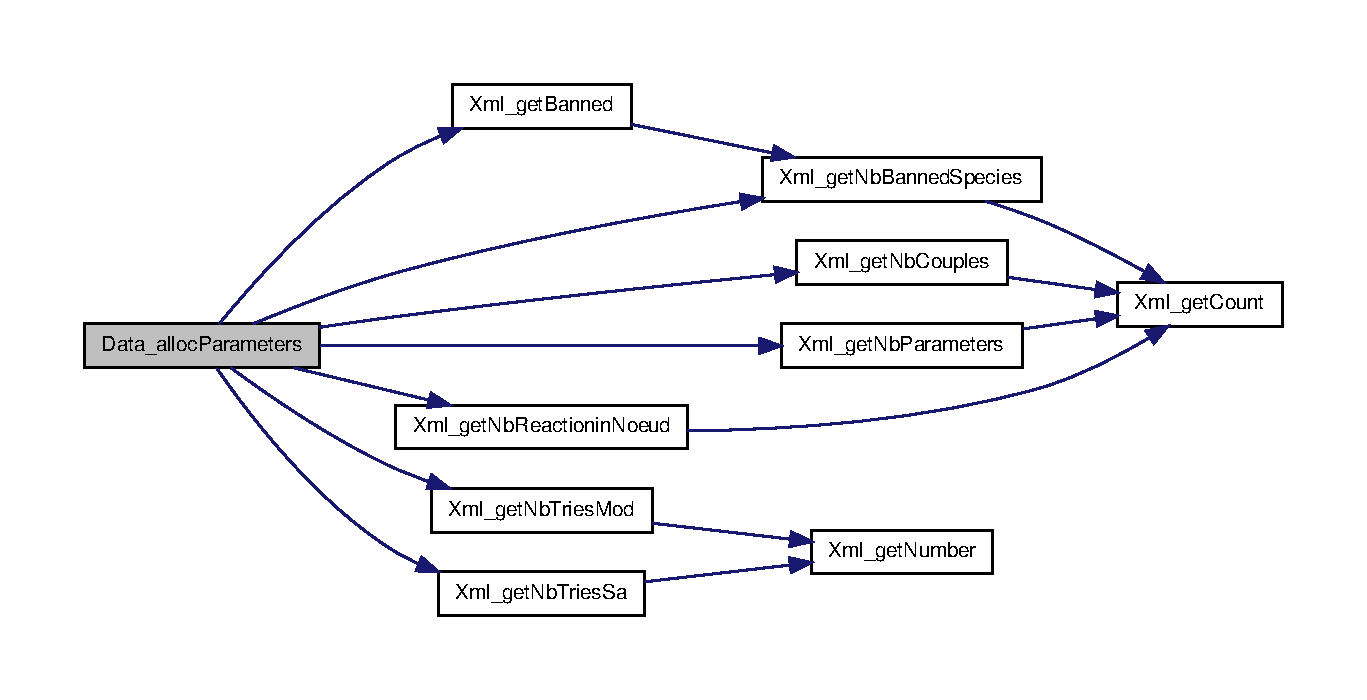
\includegraphics[width=400pt]{data__parameters_8h_ada6a0c0e47ea4e678bbd615c9371e8af_cgraph}
\end{center}
\end{figure}


\hypertarget{data__parameters_8h_a46e8fbe37a14a679690ad84c4a596cc4}{
\index{data\_\-parameters.h@{data\_\-parameters.h}!Data\_\-allocScore@{Data\_\-allocScore}}
\index{Data\_\-allocScore@{Data\_\-allocScore}!data_parameters.h@{data\_\-parameters.h}}
\subsubsection[{Data\_\-allocScore}]{\setlength{\rightskip}{0pt plus 5cm}void Data\_\-allocScore (
\begin{DoxyParamCaption}
\item[{{\bf pScore}}]{out, }
\item[{{\bf xmlConfig\_\-t} $\ast$}]{conf, }
\item[{Model\_\-t $\ast$}]{model}
\end{DoxyParamCaption}
)}}
\label{data__parameters_8h_a46e8fbe37a14a679690ad84c4a596cc4}


Copy the partial table x in the full table y. 

\begin{DoxyAuthor}{Author}
Amine Ghozlane 
\end{DoxyAuthor}

\begin{DoxyParams}{Parameters}
{\em out} & Struct \hyperlink{structScore}{Score} \\
\hline
{\em conf} & Struct \hyperlink{structxmlConfig__t}{xmlConfig\_\-t} \\
\hline
{\em model} & Model of the SBML file \\
\hline
\end{DoxyParams}


Definition at line 238 of file data\_\-parameters.c.



References Score::name, Score::nb\_\-reaction, Score::nb\_\-species, Score::quantite, Score::reaction, Score::species, Score::species\_\-amount, Score::species\_\-weight, Score::taille, Score::tailleReactions, Score::tailleSpecies, Xml\_\-getallSpeciesFinalAmount(), Xml\_\-getallSpeciesWeight(), Xml\_\-getNbReaction(), Xml\_\-getNbSpecies(), and Xml\_\-getReactionsNames().



Referenced by Data\_\-scoreAlloc(), and Data\_\-simParameters().



Here is the call graph for this function:\nopagebreak
\begin{figure}[H]
\begin{center}
\leavevmode
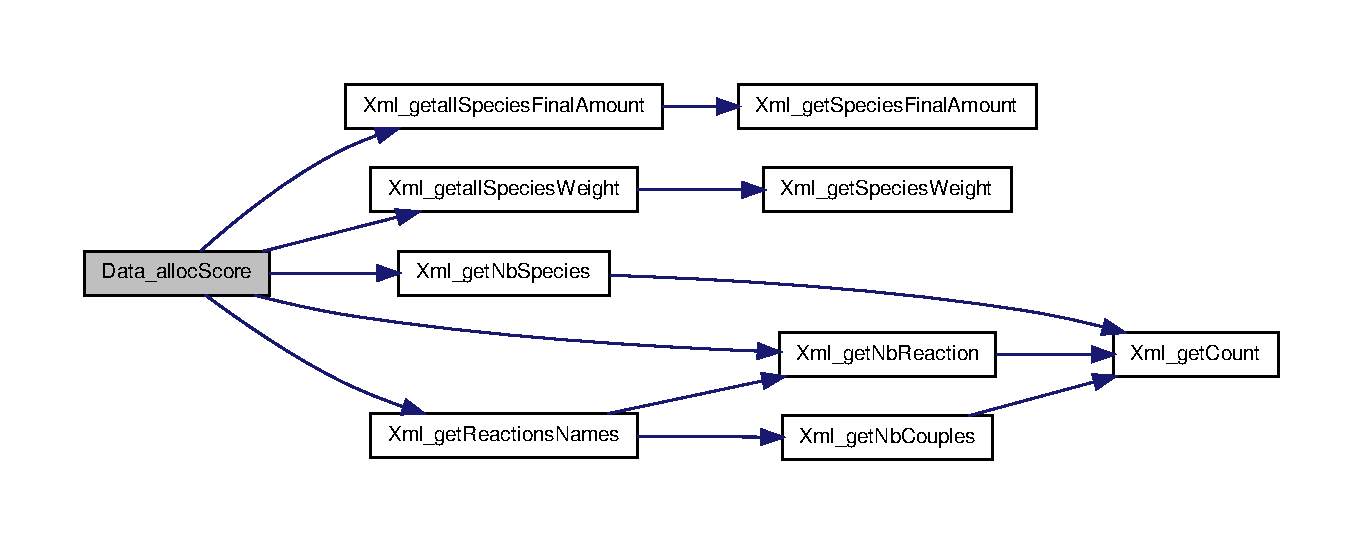
\includegraphics[width=400pt]{data__parameters_8h_a46e8fbe37a14a679690ad84c4a596cc4_cgraph}
\end{center}
\end{figure}


\hypertarget{data__parameters_8h_a7f131c19d7d1bc29db5ccf53b0517fdf}{
\index{data\_\-parameters.h@{data\_\-parameters.h}!Data\_\-allocSimParameters@{Data\_\-allocSimParameters}}
\index{Data\_\-allocSimParameters@{Data\_\-allocSimParameters}!data_parameters.h@{data\_\-parameters.h}}
\subsubsection[{Data\_\-allocSimParameters}]{\setlength{\rightskip}{0pt plus 5cm}void Data\_\-allocSimParameters (
\begin{DoxyParamCaption}
\item[{double $\ast$}]{y, }
\item[{{\bf pListParameters}}]{a}
\end{DoxyParamCaption}
)}}
\label{data__parameters_8h_a7f131c19d7d1bc29db5ccf53b0517fdf}


Allocation of tables needed for simulations. 

void \hyperlink{data__parameters_8h_a7f131c19d7d1bc29db5ccf53b0517fdf}{Data\_\-allocSimParameters(double $\ast$y, pListParameters a)} \begin{DoxyAuthor}{Author}
Amine Ghozlane 
\end{DoxyAuthor}

\begin{DoxyParams}{Parameters}
{\em y} & table of reaction parameters \\
\hline
{\em a} & Global parameters : struct \hyperlink{structListParameters}{ListParameters} \\
\hline
\end{DoxyParams}


Definition at line 391 of file data\_\-parameters.c.



References ListParameters::nb\_\-parameters.



Referenced by Data\_\-simParameters().

\hypertarget{data__parameters_8h_a27598d9ebdecd23858dc015d34daa9f8}{
\index{data\_\-parameters.h@{data\_\-parameters.h}!Data\_\-copieTab@{Data\_\-copieTab}}
\index{Data\_\-copieTab@{Data\_\-copieTab}!data_parameters.h@{data\_\-parameters.h}}
\subsubsection[{Data\_\-copieTab}]{\setlength{\rightskip}{0pt plus 5cm}int Data\_\-copieTab (
\begin{DoxyParamCaption}
\item[{{\bf pSimParameters}}]{simulated, }
\item[{double $\ast$}]{x, }
\item[{int}]{a, }
\item[{int}]{debut, }
\item[{int}]{fin}
\end{DoxyParamCaption}
)}}
\label{data__parameters_8h_a27598d9ebdecd23858dc015d34daa9f8}


Copy the partial table x in the full table y. 

\begin{DoxyAuthor}{Author}
Amine Ghozlane 
\end{DoxyAuthor}

\begin{DoxyParams}{Parameters}
{\em simulated} & Simulation parameters : struct \hyperlink{structSimParameters}{SimParameters} \\
\hline
{\em x} & Short table of reaction parameters \\
\hline
{\em a} & Line \\
\hline
{\em debut} & Beginning \\
\hline
{\em fin} & End \\
\hline
\end{DoxyParams}
\begin{DoxyReturn}{Returns}
Number of copied element 
\end{DoxyReturn}


Definition at line 347 of file data\_\-parameters.c.



References SimParameters::y.



Referenced by Data\_\-updateTab().

\hypertarget{data__parameters_8h_ab08889cc0af85b8a2e8938972107d645}{
\index{data\_\-parameters.h@{data\_\-parameters.h}!Data\_\-desallocation@{Data\_\-desallocation}}
\index{Data\_\-desallocation@{Data\_\-desallocation}!data_parameters.h@{data\_\-parameters.h}}
\subsubsection[{Data\_\-desallocation}]{\setlength{\rightskip}{0pt plus 5cm}void Data\_\-desallocation (
\begin{DoxyParamCaption}
\item[{{\bf pListParameters}}]{a}
\end{DoxyParamCaption}
)}}
\label{data__parameters_8h_ab08889cc0af85b8a2e8938972107d645}


Free memory allocated to the various objects of the program. 

\begin{DoxyAuthor}{Author}
Amine Ghozlane 
\end{DoxyAuthor}

\begin{DoxyParams}{Parameters}
{\em a} & Global parameters : struct \hyperlink{structListParameters}{ListParameters} \\
\hline
\end{DoxyParams}


Definition at line 463 of file data\_\-parameters.c.



References ListParameters::banned, ListParameters::conf, ListParameters::equation, ListParameters::model, ListParameters::nb\_\-equations, ListParameters::noeud, ListParameters::parameters, and Xml\_\-freeConfig().



Referenced by compute\_\-mpi().



Here is the call graph for this function:\nopagebreak
\begin{figure}[H]
\begin{center}
\leavevmode
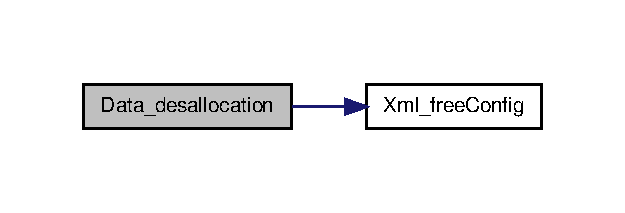
\includegraphics[width=300pt]{data__parameters_8h_ab08889cc0af85b8a2e8938972107d645_cgraph}
\end{center}
\end{figure}


\hypertarget{data__parameters_8h_a77e81e9bc2cd1ffe83bb3b8b2ecc4454}{
\index{data\_\-parameters.h@{data\_\-parameters.h}!Data\_\-desallocSim@{Data\_\-desallocSim}}
\index{Data\_\-desallocSim@{Data\_\-desallocSim}!data_parameters.h@{data\_\-parameters.h}}
\subsubsection[{Data\_\-desallocSim}]{\setlength{\rightskip}{0pt plus 5cm}void Data\_\-desallocSim (
\begin{DoxyParamCaption}
\item[{{\bf pSimParameters}}]{sim}
\end{DoxyParamCaption}
)}}
\label{data__parameters_8h_a77e81e9bc2cd1ffe83bb3b8b2ecc4454}


Free struct parameters specific to each simulation. 

\begin{DoxyAuthor}{Author}
Amine Ghozlane 
\end{DoxyAuthor}

\begin{DoxyParams}{Parameters}
{\em sim} & Simulation parameters : struct \hyperlink{structSimParameters}{SimParameters} \\
\hline
\end{DoxyParams}


Definition at line 549 of file data\_\-parameters.c.



References SimParameters::debugFile, Score::name, Score::nb\_\-reaction, SimParameters::out, Score::quantite, SimParameters::r, Score::reaction, Score::species, Score::species\_\-amount, Score::species\_\-weight, Score::taille, and SimParameters::y.



Referenced by Min\_\-compute\_\-minimization(), Mod\_\-compute\_\-modeling(), Recuit\_\-compute\_\-recuit(), and Sd\_\-compute\_\-standard\_\-deviation().

\hypertarget{data__parameters_8h_a0940064d850a6ea789bb94e0fd635d0d}{
\index{data\_\-parameters.h@{data\_\-parameters.h}!Data\_\-equationsAlloc@{Data\_\-equationsAlloc}}
\index{Data\_\-equationsAlloc@{Data\_\-equationsAlloc}!data_parameters.h@{data\_\-parameters.h}}
\subsubsection[{Data\_\-equationsAlloc}]{\setlength{\rightskip}{0pt plus 5cm}{\bf Equations}$\ast$$\ast$ Data\_\-equationsAlloc (
\begin{DoxyParamCaption}
\item[{{\bf pListParameters}}]{current, }
\item[{{\bf Equations} $\ast$$\ast$}]{pile}
\end{DoxyParamCaption}
)}}
\label{data__parameters_8h_a0940064d850a6ea789bb94e0fd635d0d}


Allocate the struct \hyperlink{structEquations}{Equations}. 

\begin{DoxyAuthor}{Author}
Amine Ghozlane 
\end{DoxyAuthor}

\begin{DoxyParams}{Parameters}
{\em current} & Current parameters : struct \hyperlink{structListParameters}{ListParameters} \\
\hline
{\em pile} & Pile des equations : struct \hyperlink{structEquations}{Equations} \\
\hline
\end{DoxyParams}
\begin{DoxyReturn}{Returns}
Allocated struct \hyperlink{structEquations}{Equations} 
\end{DoxyReturn}


Definition at line 169 of file data\_\-parameters.c.



References ListParameters::nb\_\-equations.



Referenced by Min\_\-my\_\-f(), Mod\_\-compute\_\-modeling(), Recuit\_\-energyFunction(), and Sd\_\-compute\_\-simulation().

\hypertarget{data__parameters_8h_ac0ac001f1fc3102e3ed07568cba5c570}{
\index{data\_\-parameters.h@{data\_\-parameters.h}!Data\_\-equationsInit@{Data\_\-equationsInit}}
\index{Data\_\-equationsInit@{Data\_\-equationsInit}!data_parameters.h@{data\_\-parameters.h}}
\subsubsection[{Data\_\-equationsInit}]{\setlength{\rightskip}{0pt plus 5cm}void Data\_\-equationsInit (
\begin{DoxyParamCaption}
\item[{{\bf pListParameters}}]{current, }
\item[{{\bf Equations} $\ast$$\ast$}]{pile}
\end{DoxyParamCaption}
)}}
\label{data__parameters_8h_ac0ac001f1fc3102e3ed07568cba5c570}


Initialize equations. 

\begin{DoxyAuthor}{Author}
Amine Ghozlane 
\end{DoxyAuthor}

\begin{DoxyParams}{Parameters}
{\em current} & Current parameters : struct \hyperlink{structListParameters}{ListParameters} \\
\hline
{\em pile} & Pile des equations : struct \hyperlink{structEquations}{Equations} \\
\hline
\end{DoxyParams}


Definition at line 184 of file data\_\-parameters.c.



References ListParameters::equation, Equations\_\-pileFormation(), ListParameters::nb\_\-equations, and ListParameters::noeud.



Referenced by Min\_\-my\_\-f(), Mod\_\-compute\_\-modeling(), Recuit\_\-energyFunction(), and Sd\_\-compute\_\-simulation().



Here is the call graph for this function:\nopagebreak
\begin{figure}[H]
\begin{center}
\leavevmode
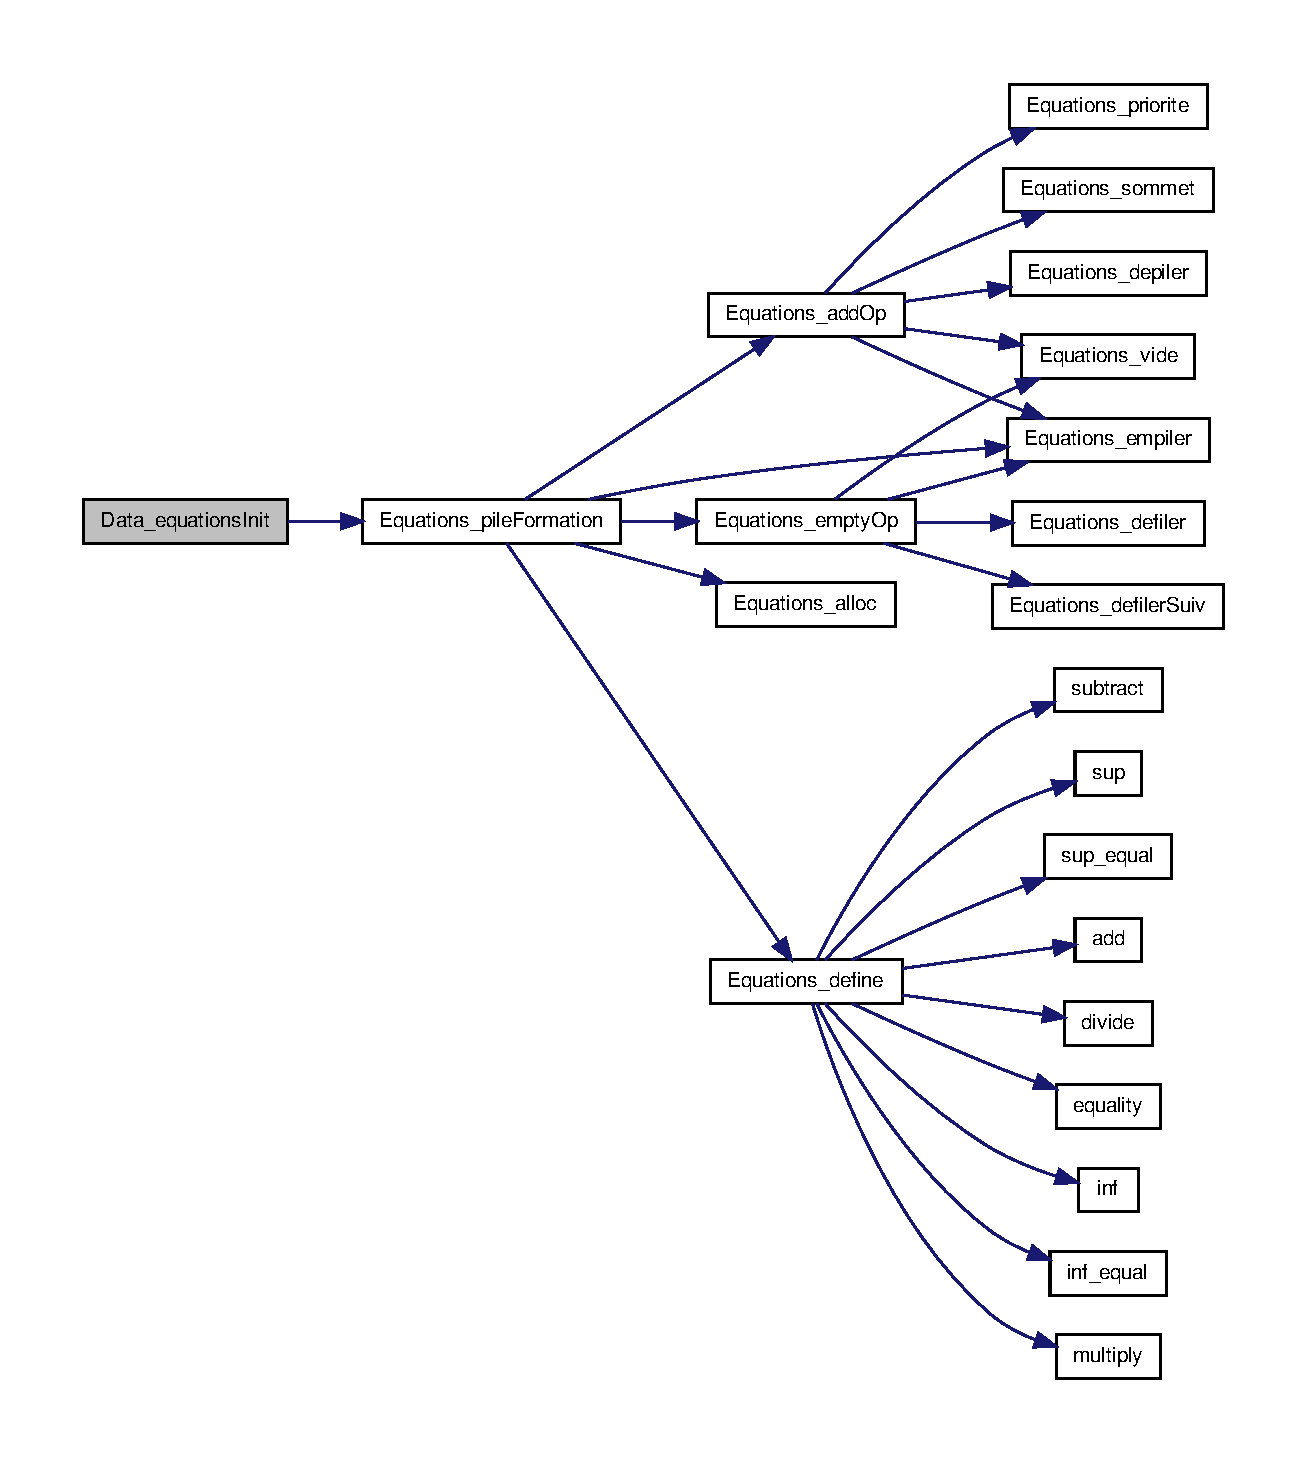
\includegraphics[width=400pt]{data__parameters_8h_ac0ac001f1fc3102e3ed07568cba5c570_cgraph}
\end{center}
\end{figure}


\hypertarget{data__parameters_8h_a2c7c500f91d49ea904f26078df0c0410}{
\index{data\_\-parameters.h@{data\_\-parameters.h}!Data\_\-initSBML@{Data\_\-initSBML}}
\index{Data\_\-initSBML@{Data\_\-initSBML}!data_parameters.h@{data\_\-parameters.h}}
\subsubsection[{Data\_\-initSBML}]{\setlength{\rightskip}{0pt plus 5cm}Model\_\-t$\ast$ Data\_\-initSBML (
\begin{DoxyParamCaption}
\item[{char $\ast$}]{sbml\_\-file}
\end{DoxyParamCaption}
)}}
\label{data__parameters_8h_a2c7c500f91d49ea904f26078df0c0410}


Load SBML file. 

\begin{DoxyAuthor}{Author}
Amine Ghozlane 
\end{DoxyAuthor}

\begin{DoxyParams}{Parameters}
{\em sbml\_\-file} & Name of the SBML file \\
\hline
\end{DoxyParams}
\begin{DoxyReturn}{Returns}
Model of the SBML file 
\end{DoxyReturn}


Definition at line 81 of file data\_\-parameters.c.



Referenced by Data\_\-parameters().

\hypertarget{data__parameters_8h_a6de2ffa5b44477da0d4a2e9e831c0c8a}{
\index{data\_\-parameters.h@{data\_\-parameters.h}!Data\_\-initXML@{Data\_\-initXML}}
\index{Data\_\-initXML@{Data\_\-initXML}!data_parameters.h@{data\_\-parameters.h}}
\subsubsection[{Data\_\-initXML}]{\setlength{\rightskip}{0pt plus 5cm}{\bf xmlConfig\_\-t}$\ast$ Data\_\-initXML (
\begin{DoxyParamCaption}
\item[{char $\ast$}]{xml\_\-file}
\end{DoxyParamCaption}
)}}
\label{data__parameters_8h_a6de2ffa5b44477da0d4a2e9e831c0c8a}


Load parameter file. 

\begin{DoxyAuthor}{Author}
Amine Ghozlane 
\end{DoxyAuthor}

\begin{DoxyParams}{Parameters}
{\em xml\_\-file} & Name of the parameter file \\
\hline
\end{DoxyParams}
\begin{DoxyReturn}{Returns}
Model of the parameter file =:Struct \hyperlink{structxmlConfig__t}{xmlConfig\_\-t} 
\end{DoxyReturn}


Definition at line 58 of file data\_\-parameters.c.



References Xml\_\-loadConfig().



Referenced by Data\_\-parameters().



Here is the call graph for this function:\nopagebreak
\begin{figure}[H]
\begin{center}
\leavevmode
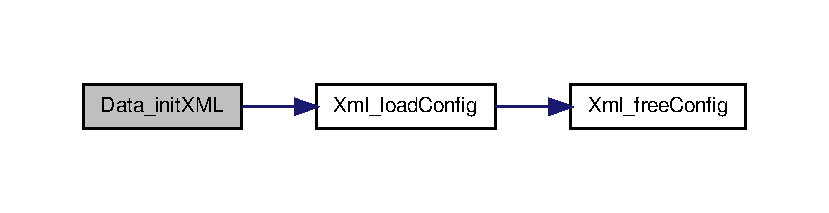
\includegraphics[width=398pt]{data__parameters_8h_a6de2ffa5b44477da0d4a2e9e831c0c8a_cgraph}
\end{center}
\end{figure}


\hypertarget{data__parameters_8h_a9cfc3bfbb7f489152efcbfa77e23bcf6}{
\index{data\_\-parameters.h@{data\_\-parameters.h}!Data\_\-parameters@{Data\_\-parameters}}
\index{Data\_\-parameters@{Data\_\-parameters}!data_parameters.h@{data\_\-parameters.h}}
\subsubsection[{Data\_\-parameters}]{\setlength{\rightskip}{0pt plus 5cm}void Data\_\-parameters (
\begin{DoxyParamCaption}
\item[{{\bf pListParameters}}]{a, }
\item[{char $\ast$$\ast$}]{files\_\-path}
\end{DoxyParamCaption}
)}}
\label{data__parameters_8h_a9cfc3bfbb7f489152efcbfa77e23bcf6}


Record parameters of the simulation. 

\begin{DoxyAuthor}{Author}
Amine Ghozlane 
\end{DoxyAuthor}

\begin{DoxyParams}{Parameters}
{\em a} & Global parameters : struct \hyperlink{structListParameters}{ListParameters} \\
\hline
{\em files\_\-path} & List of paths \\
\hline
\end{DoxyParams}


Definition at line 442 of file data\_\-parameters.c.



References ListParameters::conf, Data\_\-allocEquations(), Data\_\-allocParameters(), Data\_\-initSBML(), Data\_\-initXML(), and ListParameters::model.



Referenced by compute\_\-mpi().



Here is the call graph for this function:\nopagebreak
\begin{figure}[H]
\begin{center}
\leavevmode
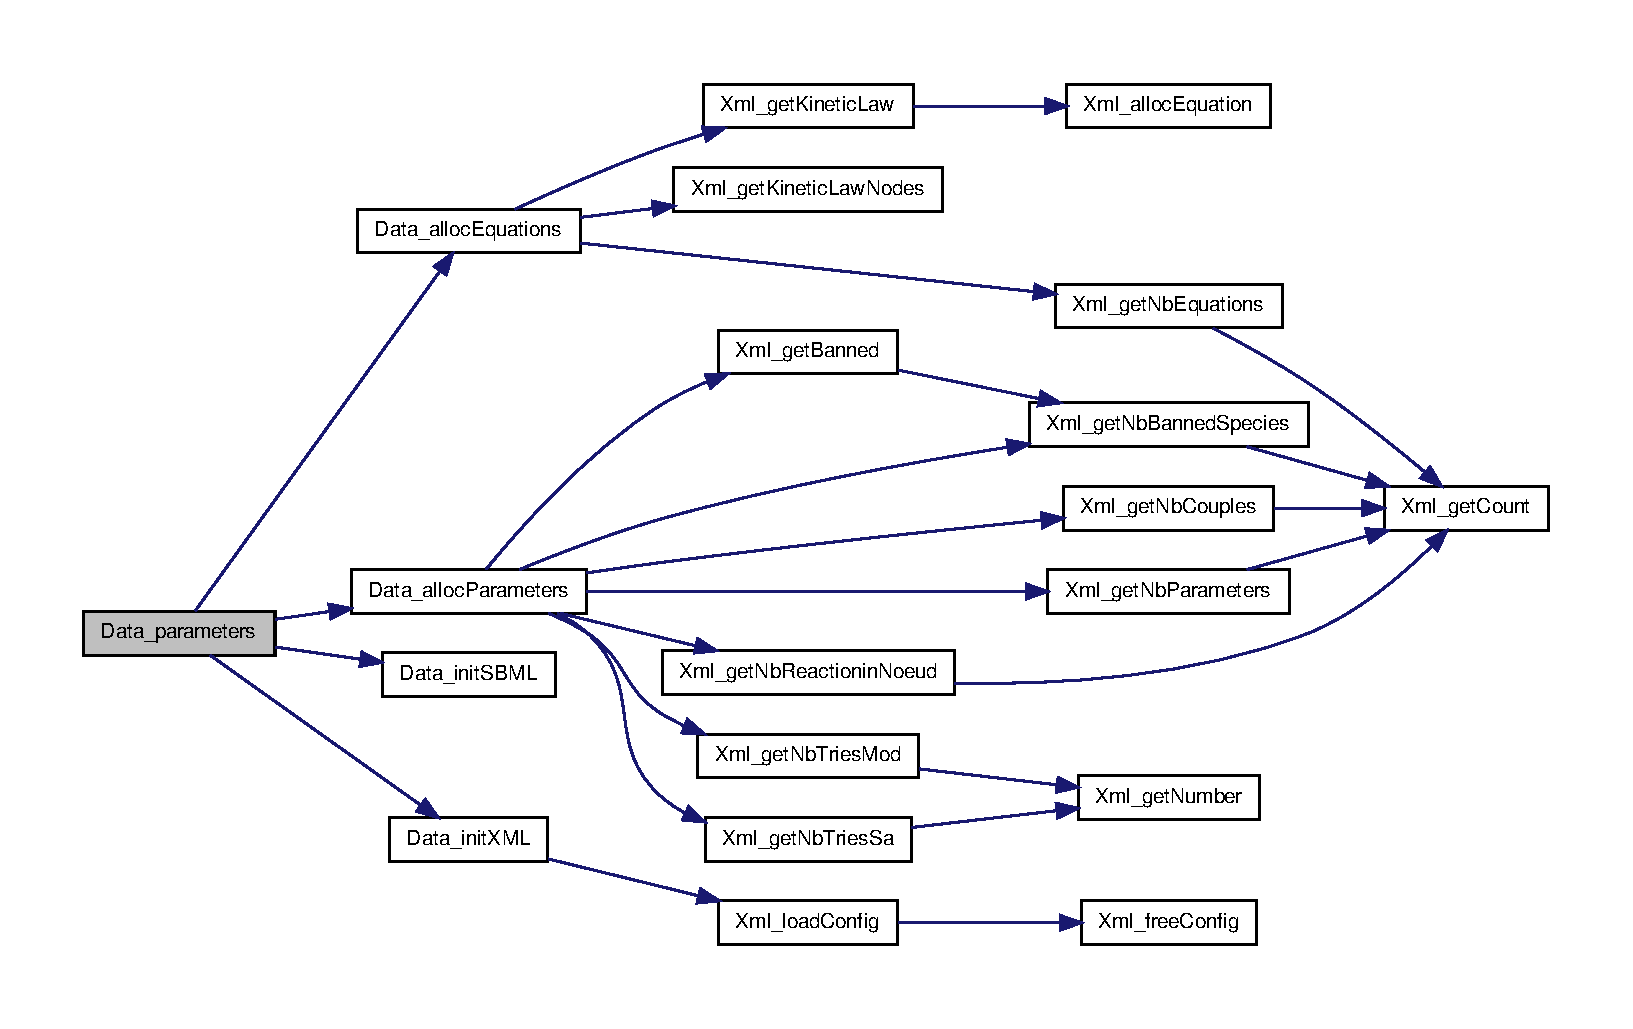
\includegraphics[width=400pt]{data__parameters_8h_a9cfc3bfbb7f489152efcbfa77e23bcf6_cgraph}
\end{center}
\end{figure}


\hypertarget{data__parameters_8h_a82ec4869c2eb338089f664171740b07b}{
\index{data\_\-parameters.h@{data\_\-parameters.h}!Data\_\-rngAlloc@{Data\_\-rngAlloc}}
\index{Data\_\-rngAlloc@{Data\_\-rngAlloc}!data_parameters.h@{data\_\-parameters.h}}
\subsubsection[{Data\_\-rngAlloc}]{\setlength{\rightskip}{0pt plus 5cm}gsl\_\-rng$\ast$ Data\_\-rngAlloc (
\begin{DoxyParamCaption}
\item[{gsl\_\-rng $\ast$}]{r}
\end{DoxyParamCaption}
)}}
\label{data__parameters_8h_a82ec4869c2eb338089f664171740b07b}


Allocation of the random number generator. 

\begin{DoxyAuthor}{Author}
Amine Ghozlane 
\end{DoxyAuthor}

\begin{DoxyParams}{Parameters}
{\em r} & Random number generator \\
\hline
\end{DoxyParams}
\begin{DoxyReturn}{Returns}
Random number generator 
\end{DoxyReturn}


Definition at line 135 of file data\_\-parameters.c.



Referenced by Data\_\-simParameters().

\hypertarget{data__parameters_8h_a28bd10646fcc4410a1d1d6433e84ea95}{
\index{data\_\-parameters.h@{data\_\-parameters.h}!Data\_\-scoreAlloc@{Data\_\-scoreAlloc}}
\index{Data\_\-scoreAlloc@{Data\_\-scoreAlloc}!data_parameters.h@{data\_\-parameters.h}}
\subsubsection[{Data\_\-scoreAlloc}]{\setlength{\rightskip}{0pt plus 5cm}{\bf pScore} Data\_\-scoreAlloc (
\begin{DoxyParamCaption}
\item[{{\bf pListParameters}}]{a}
\end{DoxyParamCaption}
)}}
\label{data__parameters_8h_a28bd10646fcc4410a1d1d6433e84ea95}


Allocation of the struct \hyperlink{structScore}{Score}. 

\begin{DoxyAuthor}{Author}
Amine Ghozlane 
\end{DoxyAuthor}

\begin{DoxyParams}{Parameters}
{\em a} & Global parameters : struct \hyperlink{structListParameters}{ListParameters} \\
\hline
\end{DoxyParams}
\begin{DoxyReturn}{Returns}
Allocated struct \hyperlink{structScore}{Score} 
\end{DoxyReturn}


Definition at line 274 of file data\_\-parameters.c.



References ListParameters::conf, Data\_\-allocScore(), and ListParameters::model.



Referenced by Min\_\-compute\_\-minimization(), Mod\_\-compute\_\-modeling(), and Recuit\_\-compute\_\-recuit().



Here is the call graph for this function:\nopagebreak
\begin{figure}[H]
\begin{center}
\leavevmode
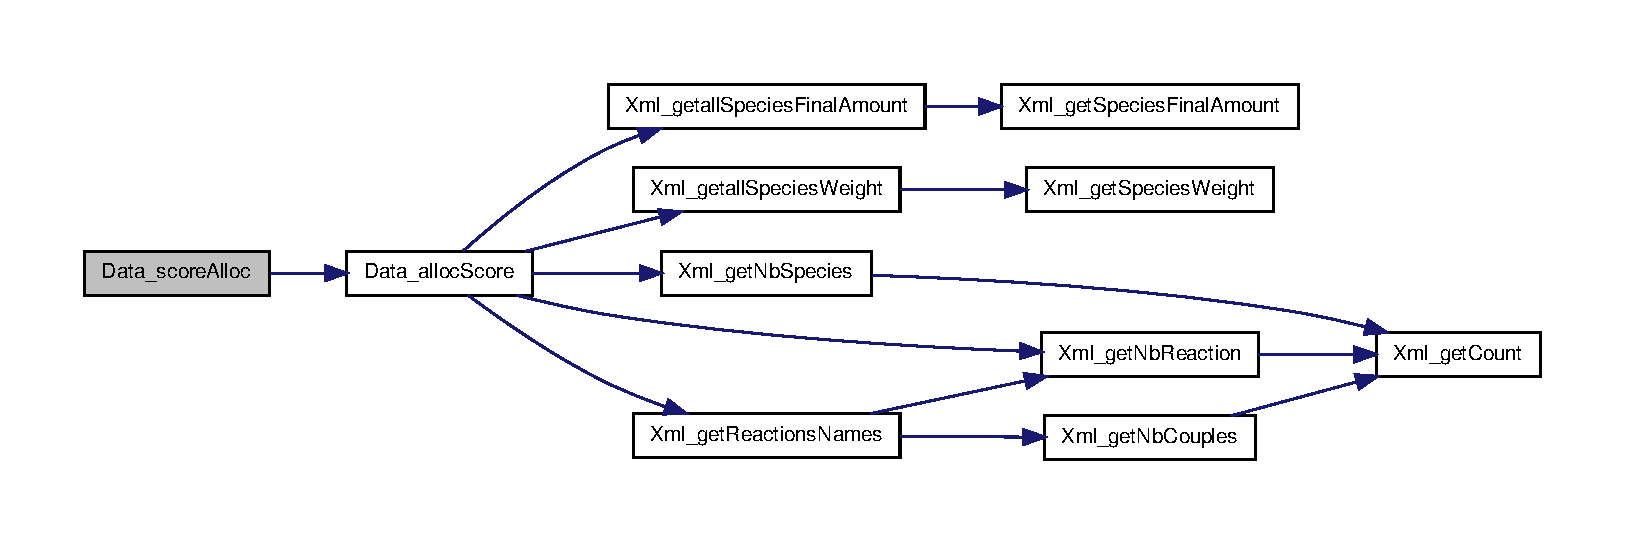
\includegraphics[width=400pt]{data__parameters_8h_a28bd10646fcc4410a1d1d6433e84ea95_cgraph}
\end{center}
\end{figure}


\hypertarget{data__parameters_8h_af65c1571388a7669aaa18c4163dac2f1}{
\index{data\_\-parameters.h@{data\_\-parameters.h}!Data\_\-scoreFree@{Data\_\-scoreFree}}
\index{Data\_\-scoreFree@{Data\_\-scoreFree}!data_parameters.h@{data\_\-parameters.h}}
\subsubsection[{Data\_\-scoreFree}]{\setlength{\rightskip}{0pt plus 5cm}void Data\_\-scoreFree (
\begin{DoxyParamCaption}
\item[{{\bf pScore}}]{out}
\end{DoxyParamCaption}
)}}
\label{data__parameters_8h_af65c1571388a7669aaa18c4163dac2f1}


Free the struct \hyperlink{structScore}{Score}. 

\begin{DoxyAuthor}{Author}
Amine Ghozlane 
\end{DoxyAuthor}

\begin{DoxyParams}{Parameters}
{\em out} & Struct score \\
\hline
\end{DoxyParams}


Definition at line 307 of file data\_\-parameters.c.



References Score::name, Score::nb\_\-reaction, Score::quantite, Score::reaction, Score::species\_\-amount, Score::species\_\-weight, and Score::taille.



Referenced by Min\_\-compute\_\-minimization(), Mod\_\-compute\_\-modeling(), and Recuit\_\-compute\_\-recuit().

\hypertarget{data__parameters_8h_a9096849f5a525ee26634b2d98a497ded}{
\index{data\_\-parameters.h@{data\_\-parameters.h}!Data\_\-scoreInit@{Data\_\-scoreInit}}
\index{Data\_\-scoreInit@{Data\_\-scoreInit}!data_parameters.h@{data\_\-parameters.h}}
\subsubsection[{Data\_\-scoreInit}]{\setlength{\rightskip}{0pt plus 5cm}void Data\_\-scoreInit (
\begin{DoxyParamCaption}
\item[{{\bf pScore}}]{out}
\end{DoxyParamCaption}
)}}
\label{data__parameters_8h_a9096849f5a525ee26634b2d98a497ded}


Initialize the struct \hyperlink{structScore}{Score}. 

\begin{DoxyAuthor}{Author}
Amine Ghozlane 
\end{DoxyAuthor}

\begin{DoxyParams}{Parameters}
{\em out} & Empty struct \hyperlink{structScore}{Score} \\
\hline
\end{DoxyParams}


Definition at line 290 of file data\_\-parameters.c.



References Score::quantite, and Score::taille.



Referenced by Min\_\-my\_\-f(), Recuit\_\-energyFunction(), and Sd\_\-compute\_\-simulation().

\hypertarget{data__parameters_8h_a2f0df5c0de22994cb0aec62dba0e1bd5}{
\index{data\_\-parameters.h@{data\_\-parameters.h}!Data\_\-simParameters@{Data\_\-simParameters}}
\index{Data\_\-simParameters@{Data\_\-simParameters}!data_parameters.h@{data\_\-parameters.h}}
\subsubsection[{Data\_\-simParameters}]{\setlength{\rightskip}{0pt plus 5cm}void Data\_\-simParameters (
\begin{DoxyParamCaption}
\item[{{\bf pListParameters}}]{a, }
\item[{{\bf pSimParameters}}]{sim, }
\item[{char $\ast$}]{out, }
\item[{char $\ast$}]{texte, }
\item[{int}]{number, }
\item[{int}]{debug}
\end{DoxyParamCaption}
)}}
\label{data__parameters_8h_a2f0df5c0de22994cb0aec62dba0e1bd5}


Recording parameters specific to each simulation. 

\begin{DoxyAuthor}{Author}
Amine Ghozlane 
\end{DoxyAuthor}

\begin{DoxyParams}{Parameters}
{\em a} & Global parameters : struct \hyperlink{structListParameters}{ListParameters} \\
\hline
{\em sim} & Simulation parameters : struct \hyperlink{structSimParameters}{SimParameters} \\
\hline
{\em out} & Output repertory \\
\hline
{\em texte} & File name \\
\hline
{\em number} & Number of the debug file \\
\hline
{\em debug} & Determine debug \\
\hline
\end{DoxyParams}


Definition at line 506 of file data\_\-parameters.c.



References ListParameters::conf, Data\_\-allocScore(), Data\_\-allocSimParameters(), Data\_\-rngAlloc(), SimParameters::debugFile, ListParameters::model, ListParameters::nb\_\-parameters, SimParameters::out, SimParameters::pile, SimParameters::r, and SimParameters::y.



Referenced by Min\_\-compute\_\-minimization(), Mod\_\-compute\_\-modeling(), Recuit\_\-compute\_\-recuit(), and Sd\_\-compute\_\-standard\_\-deviation().



Here is the call graph for this function:\nopagebreak
\begin{figure}[H]
\begin{center}
\leavevmode
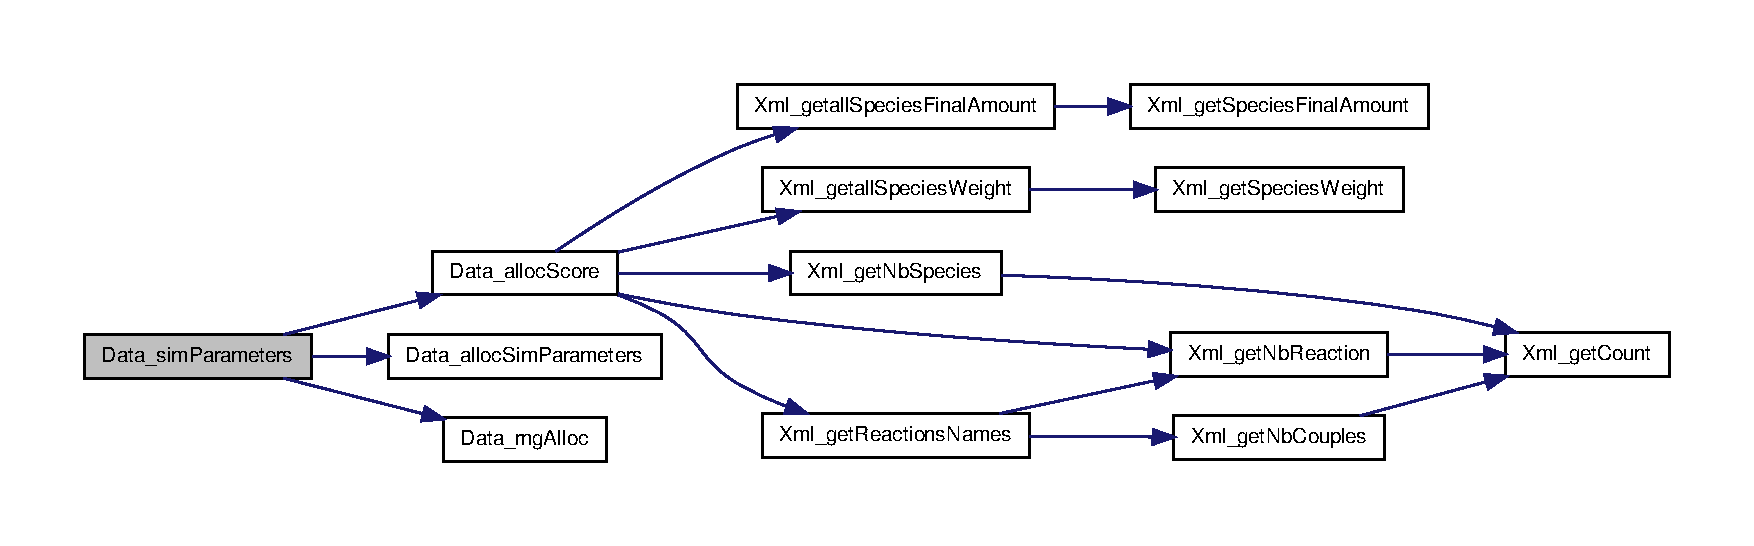
\includegraphics[width=400pt]{data__parameters_8h_a2f0df5c0de22994cb0aec62dba0e1bd5_cgraph}
\end{center}
\end{figure}


\hypertarget{data__parameters_8h_aedfc4262f7adadcd89741626ddcf0eef}{
\index{data\_\-parameters.h@{data\_\-parameters.h}!Data\_\-updateTab@{Data\_\-updateTab}}
\index{Data\_\-updateTab@{Data\_\-updateTab}!data_parameters.h@{data\_\-parameters.h}}
\subsubsection[{Data\_\-updateTab}]{\setlength{\rightskip}{0pt plus 5cm}void Data\_\-updateTab (
\begin{DoxyParamCaption}
\item[{{\bf pListParameters}}]{current, }
\item[{{\bf pSimParameters}}]{simulated, }
\item[{double $\ast$}]{x}
\end{DoxyParamCaption}
)}}
\label{data__parameters_8h_aedfc4262f7adadcd89741626ddcf0eef}


Copy table. 

\begin{DoxyAuthor}{Author}
Amine Ghozlane 
\end{DoxyAuthor}

\begin{DoxyParams}{Parameters}
{\em current} & Current parameters : struct \hyperlink{structListParameters}{ListParameters} \\
\hline
{\em simulated} & Simulation parameters : struct \hyperlink{structSimParameters}{SimParameters} \\
\hline
{\em x} & Short table of reaction parameters \\
\hline
\end{DoxyParams}


Definition at line 371 of file data\_\-parameters.c.



References Data\_\-copieTab(), ListParameters::nb\_\-couples, and ListParameters::parameters.



Referenced by Min\_\-my\_\-f(), Recuit\_\-energyFunction(), and Recuit\_\-printPosition().



Here is the call graph for this function:\nopagebreak
\begin{figure}[H]
\begin{center}
\leavevmode
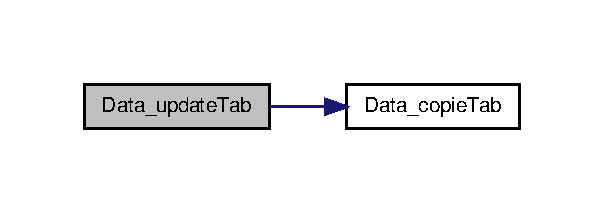
\includegraphics[width=290pt]{data__parameters_8h_aedfc4262f7adadcd89741626ddcf0eef_cgraph}
\end{center}
\end{figure}



\hypertarget{equations_8h}{
\section{metaboflux/include/equations.h File Reference}
\label{equations_8h}\index{metaboflux/include/equations.h@{metaboflux/include/equations.h}}
}


Processes an equation in MathML format.  


This graph shows which files directly or indirectly include this file:\nopagebreak
\begin{figure}[H]
\begin{center}
\leavevmode
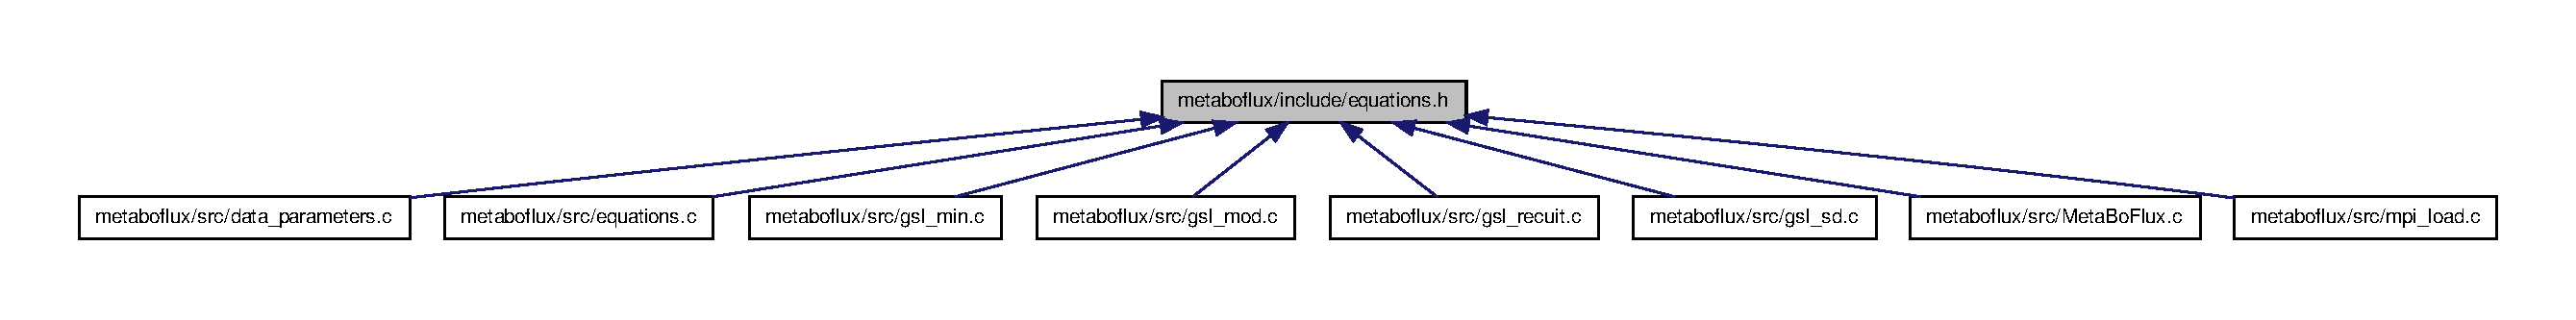
\includegraphics[width=400pt]{equations_8h__dep__incl}
\end{center}
\end{figure}
\subsection*{Data Structures}
\begin{DoxyCompactItemize}
\item 
union \hyperlink{unionEqudata}{Equdata}
\begin{DoxyCompactList}\small\item\em Equation data. \end{DoxyCompactList}\item 
struct \hyperlink{structEquations}{Equations}
\begin{DoxyCompactList}\small\item\em Function pointers used for operations. \end{DoxyCompactList}\end{DoxyCompactItemize}
\subsection*{Enumerations}
\begin{DoxyCompactItemize}
\item 
enum \hyperlink{equations_8h_adbcf1047b90fcdb0f3d285fb4a7c70d0}{Equtype} \{ \par
\hyperlink{equations_8h_adbcf1047b90fcdb0f3d285fb4a7c70d0a995640a12d5339aabee76a933fb5f519}{constant}, 
\hyperlink{equations_8h_adbcf1047b90fcdb0f3d285fb4a7c70d0ac8bb815d8e3574231fdd28645507fdaf}{variable}, 
\hyperlink{equations_8h_adbcf1047b90fcdb0f3d285fb4a7c70d0adbbc94ea3351977e33fa1a1d9dfc458f}{addition}, 
\hyperlink{equations_8h_adbcf1047b90fcdb0f3d285fb4a7c70d0a6ac6588349b6a4df159905733d74a8b0}{soustraction}, 
\par
\hyperlink{equations_8h_adbcf1047b90fcdb0f3d285fb4a7c70d0a5cadaaaf2f12196ff90d101dbcb07287}{multiplication}, 
\hyperlink{equations_8h_adbcf1047b90fcdb0f3d285fb4a7c70d0af91a7893f9d938f7eb36433f93f99f26}{division}, 
\hyperlink{equations_8h_adbcf1047b90fcdb0f3d285fb4a7c70d0ab5800e866b0cfbd93e858c68a8246c27}{equal}, 
\hyperlink{equations_8h_adbcf1047b90fcdb0f3d285fb4a7c70d0a4461fc80cd8d4d479e0f9d26052c81b0}{superior}, 
\par
\hyperlink{equations_8h_adbcf1047b90fcdb0f3d285fb4a7c70d0a9e2d529f48f9a4c5234363cb003fdd7b}{superior\_\-equal}, 
\hyperlink{equations_8h_adbcf1047b90fcdb0f3d285fb4a7c70d0aa26fb260205509c6b988d10a315646c8}{inferior}, 
\hyperlink{equations_8h_adbcf1047b90fcdb0f3d285fb4a7c70d0a3e2f2ede1bcb2b6276d52c9ed64c4a8c}{inferior\_\-equal}
 \}
\begin{DoxyCompactList}\small\item\em Operation constants. \end{DoxyCompactList}\end{DoxyCompactItemize}
\subsection*{Functions}
\begin{DoxyCompactItemize}
\item 
double \hyperlink{equations_8h_abaee43b91c808de325abcfa4cf1b6698}{add} (double, double)
\begin{DoxyCompactList}\small\item\em Add two numbers. \end{DoxyCompactList}\item 
double \hyperlink{equations_8h_a8c90ae25e75adcfeeaf307cc2df2f360}{subtract} (double, double)
\begin{DoxyCompactList}\small\item\em Subtraction two numbers. \end{DoxyCompactList}\item 
double \hyperlink{equations_8h_a6081051f0fa134ecbd577740cbb92220}{multiply} (double, double)
\begin{DoxyCompactList}\small\item\em Multiply two numbers. \end{DoxyCompactList}\item 
double \hyperlink{equations_8h_a004a98a2cd96d70101b27be400dc4a5c}{divide} (double, double)
\begin{DoxyCompactList}\small\item\em Divide two numbers. \end{DoxyCompactList}\item 
double \hyperlink{equations_8h_ae22300bfd59f7b0a12d56b5cb32b9429}{equality} (double, double)
\begin{DoxyCompactList}\small\item\em Test the equality of two numbers. \end{DoxyCompactList}\item 
double \hyperlink{equations_8h_a0ce3f625ded68dd2b0a927b1c3d85471}{sup} (double, double)
\begin{DoxyCompactList}\small\item\em Test the superiority between two numbers. \end{DoxyCompactList}\item 
double \hyperlink{equations_8h_a26bbff8f2c38ba14fea7a9d6067329b2}{sup\_\-equal} (double, double)
\begin{DoxyCompactList}\small\item\em Test the superiority or equality between two numbers. \end{DoxyCompactList}\item 
double \hyperlink{equations_8h_a3a5c2f0eec28c21db099d689bbcc5b14}{inf} (double, double)
\begin{DoxyCompactList}\small\item\em Test the inferiority between two numbers. \end{DoxyCompactList}\item 
double \hyperlink{equations_8h_aa6c076aacdfbdd13d6f25e0f36d6406b}{inf\_\-equal} (double, double)
\begin{DoxyCompactList}\small\item\em Test the inferiority or equality between two numbers. \end{DoxyCompactList}\item 
\hyperlink{structEquations}{pEquations} \hyperlink{equations_8h_a977051374a319d6bd60ef8ca2c03c952}{Equations\_\-alloc} (void)
\begin{DoxyCompactList}\small\item\em Alloc memory and initialize the struct \hyperlink{structEquations}{Equations}. \end{DoxyCompactList}\item 
void \hyperlink{equations_8h_afa3dcf131c38609646bd0ff79aef41d7}{Equations\_\-define} (\hyperlink{structEquations}{pEquations}, char $\ast$)
\begin{DoxyCompactList}\small\item\em Identify the mathematical operator used. \end{DoxyCompactList}\item 
int \hyperlink{equations_8h_a7aa0efc05d71c770b8aaf4ad6d677be2}{Equations\_\-vide} (\hyperlink{structEquations}{pEquations})
\begin{DoxyCompactList}\small\item\em Test if the struct \hyperlink{structEquations}{Equations} is empty. \end{DoxyCompactList}\item 
\hyperlink{structEquations}{pEquations} \hyperlink{equations_8h_ab8d4e4c2f309e68abe8dbcae96a240d5}{Equations\_\-empiler} (\hyperlink{structEquations}{pEquations}, \hyperlink{structEquations}{pEquations})
\begin{DoxyCompactList}\small\item\em Stack an element to the struct \hyperlink{structEquations}{Equations}. \end{DoxyCompactList}\item 
\hyperlink{structEquations}{pEquations} \hyperlink{equations_8h_ae69932ae59f7f39d19b16efdcd0ba814}{Equations\_\-depiler} (\hyperlink{structEquations}{pEquations})
\begin{DoxyCompactList}\small\item\em Unstack the last element of the struct \hyperlink{structEquations}{Equations}. \end{DoxyCompactList}\item 
\hyperlink{structEquations}{pEquations} \hyperlink{equations_8h_a25cc9b41f25936e9d67a650554dc875d}{Equations\_\-sommet} (\hyperlink{structEquations}{pEquations})
\begin{DoxyCompactList}\small\item\em Look for the last element of the struct \hyperlink{structEquations}{Equations}. \end{DoxyCompactList}\item 
\hyperlink{structEquations}{pEquations} \hyperlink{equations_8h_a7b5cc03bbac246e28d61714dc2931a92}{Equations\_\-defiler} (\hyperlink{structEquations}{pEquations})
\begin{DoxyCompactList}\small\item\em Look for the first element of the struct \hyperlink{structEquations}{Equations}. \end{DoxyCompactList}\item 
\hyperlink{structEquations}{pEquations} \hyperlink{equations_8h_a2c6acfd549462cb3be5a53775767429a}{Equations\_\-defilerSuiv} (\hyperlink{structEquations}{pEquations})
\begin{DoxyCompactList}\small\item\em Get the next element of the struct \hyperlink{structEquations}{Equations}. \end{DoxyCompactList}\item 
int \hyperlink{equations_8h_a9107be336f525ee8ee8bb0d56bc91d8b}{Equations\_\-priorite} (\hyperlink{structEquations}{pEquations})
\begin{DoxyCompactList}\small\item\em Give the priority of the operator. Multiplication and Division have higher priority than addition or subtration... \end{DoxyCompactList}\item 
void \hyperlink{equations_8h_ab5545fa4c945c64285e91687d90767f4}{Equations\_\-print} (\hyperlink{structEquations}{pEquations})
\begin{DoxyCompactList}\small\item\em Print all information on the element of the struct \hyperlink{structEquations}{Equations}. \end{DoxyCompactList}\item 
\hyperlink{structEquations}{pEquations} \hyperlink{equations_8h_aa1fb3994a7c6fdf69e7aab84414f467c}{Equations\_\-addOp} (\hyperlink{structEquations}{pEquations}, \hyperlink{structEquations}{pEquations}, \hyperlink{structEquations}{pEquations})
\begin{DoxyCompactList}\small\item\em Build the list of the Struct \hyperlink{structEquations}{Equations} result used to compute the equation. \end{DoxyCompactList}\item 
void \hyperlink{equations_8h_ae188053c785ea42afda7a9a604140b44}{Equations\_\-emptyOp} (\hyperlink{structEquations}{pEquations}, \hyperlink{structEquations}{pEquations})
\begin{DoxyCompactList}\small\item\em Empty the Struct \hyperlink{structEquations}{Equations} op for the struct Equation result. \end{DoxyCompactList}\item 
\hyperlink{structEquations}{pEquations} \hyperlink{equations_8h_ae0f5b302dbd7d0bb1524b48aa38bec6c}{Equations\_\-pileFormation} (char $\ast$$\ast$$\ast$, int)
\begin{DoxyCompactList}\small\item\em Build pile. \end{DoxyCompactList}\item 
double \hyperlink{equations_8h_acacabe612b4e956d3db6d1677dac4037}{Equations\_\-findSpecies} (char $\ast$, char $\ast$$\ast$, double $\ast$, int)
\begin{DoxyCompactList}\small\item\em Look for the quantity of a molecule in the list. \end{DoxyCompactList}\item 
double \hyperlink{equations_8h_af09f4513d82b106e8e9157f30c909529}{Equations\_\-resultat} (\hyperlink{structEquations}{pEquations}, \hyperlink{structEquations}{pEquations}, \hyperlink{structEquations}{pEquations}, char $\ast$$\ast$, double $\ast$, int)
\begin{DoxyCompactList}\small\item\em Compute the result of two pile. \end{DoxyCompactList}\item 
double \hyperlink{equations_8h_a6e6af023dd85b15e2af2129a5c857238}{Equations\_\-calcul} (\hyperlink{structEquations}{pEquations}, char $\ast$$\ast$, double $\ast$, int)
\begin{DoxyCompactList}\small\item\em Compute the score of the equation. \end{DoxyCompactList}\item 
double \hyperlink{equations_8h_a543044646be5d2086c3301f7db2a0c1f}{Equations\_\-finalQuantite} (int, char $\ast$$\ast$, int $\ast$, int $\ast$, char $\ast$$\ast$, double $\ast$, int)
\begin{DoxyCompactList}\small\item\em Compute the score of the quantity which means the difference between what is expected to what is simulated. \end{DoxyCompactList}\end{DoxyCompactItemize}


\subsection{Detailed Description}
Processes an equation in MathML format. This file is part of MetaBoFlux (\href{http://www.cbib.u-bordeaux2.fr/metaboflux/}{\tt http://www.cbib.u-\/bordeaux2.fr/metaboflux/}) Copyright (C) 2010 Amine Ghozlane from LaBRI and University of Bordeaux 1

MetaBoFlux is free software: you can redistribute it and/or modify it under the terms of the GNU Lesser General Public License as published by the Free Software Foundation, either version 3 of the License, or (at your option) any later version.

MetaBoFlux is distributed in the hope that it will be useful, but WITHOUT ANY WARRANTY; without even the implied warranty of MERCHANTABILITY or FITNESS FOR A PARTICULAR PURPOSE. See the GNU General Public License for more details.

You should have received a copy of the GNU Lesser General Public License along with this program. If not, see $<$\href{http://www.gnu.org/licenses/}{\tt http://www.gnu.org/licenses/}$>$.

\begin{DoxyAuthor}{Author}
\{Amine Ghozlane\} 
\end{DoxyAuthor}
\begin{DoxyVersion}{Version}
2.0 
\end{DoxyVersion}
\begin{DoxyDate}{Date}
15 janvier 2010 
\end{DoxyDate}


Definition in file \hyperlink{equations_8h_source}{equations.h}.



\subsection{Enumeration Type Documentation}
\hypertarget{equations_8h_adbcf1047b90fcdb0f3d285fb4a7c70d0}{
\index{equations.h@{equations.h}!Equtype@{Equtype}}
\index{Equtype@{Equtype}!equations.h@{equations.h}}
\subsubsection[{Equtype}]{\setlength{\rightskip}{0pt plus 5cm}enum {\bf Equtype}}}
\label{equations_8h_adbcf1047b90fcdb0f3d285fb4a7c70d0}


Operation constants. 

Equtype is a set of predefined constants for the different operators. \begin{Desc}
\item[Enumerator: ]\par
\begin{description}
\index{constant@{constant}!equations.h@{equations.h}}\index{equations.h@{equations.h}!constant@{constant}}\item[{\em 
\hypertarget{equations_8h_adbcf1047b90fcdb0f3d285fb4a7c70d0a995640a12d5339aabee76a933fb5f519}{
constant}
\label{equations_8h_adbcf1047b90fcdb0f3d285fb4a7c70d0a995640a12d5339aabee76a933fb5f519}
}]Constant \index{variable@{variable}!equations.h@{equations.h}}\index{equations.h@{equations.h}!variable@{variable}}\item[{\em 
\hypertarget{equations_8h_adbcf1047b90fcdb0f3d285fb4a7c70d0ac8bb815d8e3574231fdd28645507fdaf}{
variable}
\label{equations_8h_adbcf1047b90fcdb0f3d285fb4a7c70d0ac8bb815d8e3574231fdd28645507fdaf}
}]Variable : ex. transition\_\-x ... \index{addition@{addition}!equations.h@{equations.h}}\index{equations.h@{equations.h}!addition@{addition}}\item[{\em 
\hypertarget{equations_8h_adbcf1047b90fcdb0f3d285fb4a7c70d0adbbc94ea3351977e33fa1a1d9dfc458f}{
addition}
\label{equations_8h_adbcf1047b90fcdb0f3d285fb4a7c70d0adbbc94ea3351977e33fa1a1d9dfc458f}
}]Addition \index{soustraction@{soustraction}!equations.h@{equations.h}}\index{equations.h@{equations.h}!soustraction@{soustraction}}\item[{\em 
\hypertarget{equations_8h_adbcf1047b90fcdb0f3d285fb4a7c70d0a6ac6588349b6a4df159905733d74a8b0}{
soustraction}
\label{equations_8h_adbcf1047b90fcdb0f3d285fb4a7c70d0a6ac6588349b6a4df159905733d74a8b0}
}]Substraction \index{multiplication@{multiplication}!equations.h@{equations.h}}\index{equations.h@{equations.h}!multiplication@{multiplication}}\item[{\em 
\hypertarget{equations_8h_adbcf1047b90fcdb0f3d285fb4a7c70d0a5cadaaaf2f12196ff90d101dbcb07287}{
multiplication}
\label{equations_8h_adbcf1047b90fcdb0f3d285fb4a7c70d0a5cadaaaf2f12196ff90d101dbcb07287}
}]Multiply \index{division@{division}!equations.h@{equations.h}}\index{equations.h@{equations.h}!division@{division}}\item[{\em 
\hypertarget{equations_8h_adbcf1047b90fcdb0f3d285fb4a7c70d0af91a7893f9d938f7eb36433f93f99f26}{
division}
\label{equations_8h_adbcf1047b90fcdb0f3d285fb4a7c70d0af91a7893f9d938f7eb36433f93f99f26}
}]Divide \index{equal@{equal}!equations.h@{equations.h}}\index{equations.h@{equations.h}!equal@{equal}}\item[{\em 
\hypertarget{equations_8h_adbcf1047b90fcdb0f3d285fb4a7c70d0ab5800e866b0cfbd93e858c68a8246c27}{
equal}
\label{equations_8h_adbcf1047b90fcdb0f3d285fb4a7c70d0ab5800e866b0cfbd93e858c68a8246c27}
}]Equality \index{superior@{superior}!equations.h@{equations.h}}\index{equations.h@{equations.h}!superior@{superior}}\item[{\em 
\hypertarget{equations_8h_adbcf1047b90fcdb0f3d285fb4a7c70d0a4461fc80cd8d4d479e0f9d26052c81b0}{
superior}
\label{equations_8h_adbcf1047b90fcdb0f3d285fb4a7c70d0a4461fc80cd8d4d479e0f9d26052c81b0}
}]Superiority \index{superior\_\-equal@{superior\_\-equal}!equations.h@{equations.h}}\index{equations.h@{equations.h}!superior\_\-equal@{superior\_\-equal}}\item[{\em 
\hypertarget{equations_8h_adbcf1047b90fcdb0f3d285fb4a7c70d0a9e2d529f48f9a4c5234363cb003fdd7b}{
superior\_\-equal}
\label{equations_8h_adbcf1047b90fcdb0f3d285fb4a7c70d0a9e2d529f48f9a4c5234363cb003fdd7b}
}]Sup\_\-equality \index{inferior@{inferior}!equations.h@{equations.h}}\index{equations.h@{equations.h}!inferior@{inferior}}\item[{\em 
\hypertarget{equations_8h_adbcf1047b90fcdb0f3d285fb4a7c70d0aa26fb260205509c6b988d10a315646c8}{
inferior}
\label{equations_8h_adbcf1047b90fcdb0f3d285fb4a7c70d0aa26fb260205509c6b988d10a315646c8}
}]Inferiority \index{inferior\_\-equal@{inferior\_\-equal}!equations.h@{equations.h}}\index{equations.h@{equations.h}!inferior\_\-equal@{inferior\_\-equal}}\item[{\em 
\hypertarget{equations_8h_adbcf1047b90fcdb0f3d285fb4a7c70d0a3e2f2ede1bcb2b6276d52c9ed64c4a8c}{
inferior\_\-equal}
\label{equations_8h_adbcf1047b90fcdb0f3d285fb4a7c70d0a3e2f2ede1bcb2b6276d52c9ed64c4a8c}
}]Inf\_\-equality \end{description}
\end{Desc}



Definition at line 38 of file equations.h.



\subsection{Function Documentation}
\hypertarget{equations_8h_abaee43b91c808de325abcfa4cf1b6698}{
\index{equations.h@{equations.h}!add@{add}}
\index{add@{add}!equations.h@{equations.h}}
\subsubsection[{add}]{\setlength{\rightskip}{0pt plus 5cm}double add (
\begin{DoxyParamCaption}
\item[{double}]{arg1, }
\item[{double}]{arg2}
\end{DoxyParamCaption}
)}}
\label{equations_8h_abaee43b91c808de325abcfa4cf1b6698}


Add two numbers. 

\begin{DoxyAuthor}{Author}
Amine Ghozlane 
\end{DoxyAuthor}

\begin{DoxyParams}{Parameters}
{\em arg1} & Value 1 \\
\hline
{\em arg2} & Value 2 \\
\hline
\end{DoxyParams}
\begin{DoxyReturn}{Returns}
Result 
\end{DoxyReturn}


Definition at line 43 of file equations.c.



Referenced by Equations\_\-define().

\hypertarget{equations_8h_a004a98a2cd96d70101b27be400dc4a5c}{
\index{equations.h@{equations.h}!divide@{divide}}
\index{divide@{divide}!equations.h@{equations.h}}
\subsubsection[{divide}]{\setlength{\rightskip}{0pt plus 5cm}double divide (
\begin{DoxyParamCaption}
\item[{double}]{arg1, }
\item[{double}]{arg2}
\end{DoxyParamCaption}
)}}
\label{equations_8h_a004a98a2cd96d70101b27be400dc4a5c}


Divide two numbers. 

\begin{DoxyAuthor}{Author}
Amine Ghozlane 
\end{DoxyAuthor}

\begin{DoxyParams}{Parameters}
{\em arg1} & Value 1 \\
\hline
{\em arg2} & Value 2 \\
\hline
\end{DoxyParams}
\begin{DoxyReturn}{Returns}
Result 
\end{DoxyReturn}


Definition at line 82 of file equations.c.



Referenced by Equations\_\-define().

\hypertarget{equations_8h_ae22300bfd59f7b0a12d56b5cb32b9429}{
\index{equations.h@{equations.h}!equality@{equality}}
\index{equality@{equality}!equations.h@{equations.h}}
\subsubsection[{equality}]{\setlength{\rightskip}{0pt plus 5cm}double equality (
\begin{DoxyParamCaption}
\item[{double}]{arg1, }
\item[{double}]{arg2}
\end{DoxyParamCaption}
)}}
\label{equations_8h_ae22300bfd59f7b0a12d56b5cb32b9429}


Test the equality of two numbers. 

\begin{DoxyAuthor}{Author}
Amine Ghozlane 
\end{DoxyAuthor}

\begin{DoxyParams}{Parameters}
{\em arg1} & Value 1 \\
\hline
{\em arg2} & Value 2 \\
\hline
\end{DoxyParams}
\begin{DoxyReturn}{Returns}
Result 
\end{DoxyReturn}


Definition at line 95 of file equations.c.



Referenced by Equations\_\-define().

\hypertarget{equations_8h_aa1fb3994a7c6fdf69e7aab84414f467c}{
\index{equations.h@{equations.h}!Equations\_\-addOp@{Equations\_\-addOp}}
\index{Equations\_\-addOp@{Equations\_\-addOp}!equations.h@{equations.h}}
\subsubsection[{Equations\_\-addOp}]{\setlength{\rightskip}{0pt plus 5cm}{\bf pEquations} Equations\_\-addOp (
\begin{DoxyParamCaption}
\item[{{\bf pEquations}}]{result, }
\item[{{\bf pEquations}}]{op, }
\item[{{\bf pEquations}}]{new}
\end{DoxyParamCaption}
)}}
\label{equations_8h_aa1fb3994a7c6fdf69e7aab84414f467c}


Build the list of the Struct \hyperlink{structEquations}{Equations} result used to compute the equation. 

\begin{DoxyAuthor}{Author}
Amine Ghozlane 
\end{DoxyAuthor}

\begin{DoxyParams}{Parameters}
{\em result} & Struct \hyperlink{structEquations}{Equations} used for computation \\
\hline
{\em op} & Struct \hyperlink{structEquations}{Equations} used to store the operator \\
\hline
{\em new} & One element of the Struct \hyperlink{structEquations}{Equations} \\
\hline
\end{DoxyParams}
\begin{DoxyReturn}{Returns}
List of operator 
\end{DoxyReturn}


Definition at line 383 of file equations.c.



References equal, Equations\_\-depiler(), Equations\_\-empiler(), Equations\_\-priorite(), Equations\_\-sommet(), Equations\_\-vide(), inferior, inferior\_\-equal, superior, and superior\_\-equal.



Referenced by Equations\_\-pileFormation().



Here is the call graph for this function:\nopagebreak
\begin{figure}[H]
\begin{center}
\leavevmode
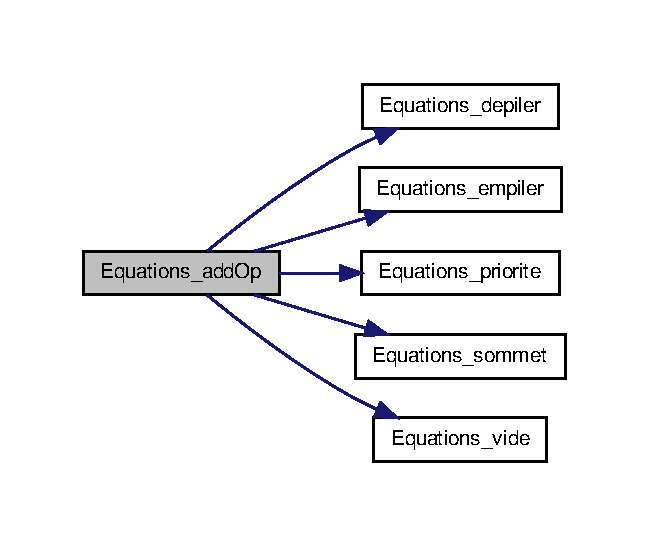
\includegraphics[width=312pt]{equations_8h_aa1fb3994a7c6fdf69e7aab84414f467c_cgraph}
\end{center}
\end{figure}


\hypertarget{equations_8h_a977051374a319d6bd60ef8ca2c03c952}{
\index{equations.h@{equations.h}!Equations\_\-alloc@{Equations\_\-alloc}}
\index{Equations\_\-alloc@{Equations\_\-alloc}!equations.h@{equations.h}}
\subsubsection[{Equations\_\-alloc}]{\setlength{\rightskip}{0pt plus 5cm}{\bf pEquations} Equations\_\-alloc (
\begin{DoxyParamCaption}
\item[{void}]{}
\end{DoxyParamCaption}
)}}
\label{equations_8h_a977051374a319d6bd60ef8ca2c03c952}


Alloc memory and initialize the struct \hyperlink{structEquations}{Equations}. 

\begin{DoxyAuthor}{Author}
Amine Ghozlane 
\end{DoxyAuthor}
\begin{DoxyReturn}{Returns}
Allocated struct \hyperlink{structEquations}{Equations} 
\end{DoxyReturn}


Definition at line 158 of file equations.c.



Referenced by Equations\_\-calcul(), and Equations\_\-pileFormation().

\hypertarget{equations_8h_a6e6af023dd85b15e2af2129a5c857238}{
\index{equations.h@{equations.h}!Equations\_\-calcul@{Equations\_\-calcul}}
\index{Equations\_\-calcul@{Equations\_\-calcul}!equations.h@{equations.h}}
\subsubsection[{Equations\_\-calcul}]{\setlength{\rightskip}{0pt plus 5cm}double Equations\_\-calcul (
\begin{DoxyParamCaption}
\item[{{\bf pEquations}}]{liste, }
\item[{char $\ast$$\ast$}]{name, }
\item[{double $\ast$}]{quantite, }
\item[{int}]{taille}
\end{DoxyParamCaption}
)}}
\label{equations_8h_a6e6af023dd85b15e2af2129a5c857238}


Compute the score of the equation. 

\begin{DoxyAuthor}{Author}
Amine Ghozlane 
\end{DoxyAuthor}

\begin{DoxyParams}{Parameters}
{\em liste} & pile of type Struct \hyperlink{structEquations}{Equations} \\
\hline
{\em name} & List of molecules \\
\hline
{\em quantite} & List of the quantity of the molecules \\
\hline
{\em taille} & Number of molecules in the list \\
\hline
\end{DoxyParams}
\begin{DoxyReturn}{Returns}
Result of the equation (First part of the energy) 
\end{DoxyReturn}


Definition at line 614 of file equations.c.



References addition, constant, division, equal, Equations\_\-alloc(), Equations\_\-defiler(), Equations\_\-defilerSuiv(), Equations\_\-depiler(), Equations\_\-empiler(), Equations\_\-extractData(), Equations\_\-resultat(), Equations\_\-vide(), inferior, inferior\_\-equal, multiplication, soustraction, superior, and superior\_\-equal.



Referenced by Min\_\-my\_\-f(), Mod\_\-compute\_\-modeling(), Recuit\_\-energyFunction(), and Sd\_\-compute\_\-simulation().



Here is the call graph for this function:\nopagebreak
\begin{figure}[H]
\begin{center}
\leavevmode
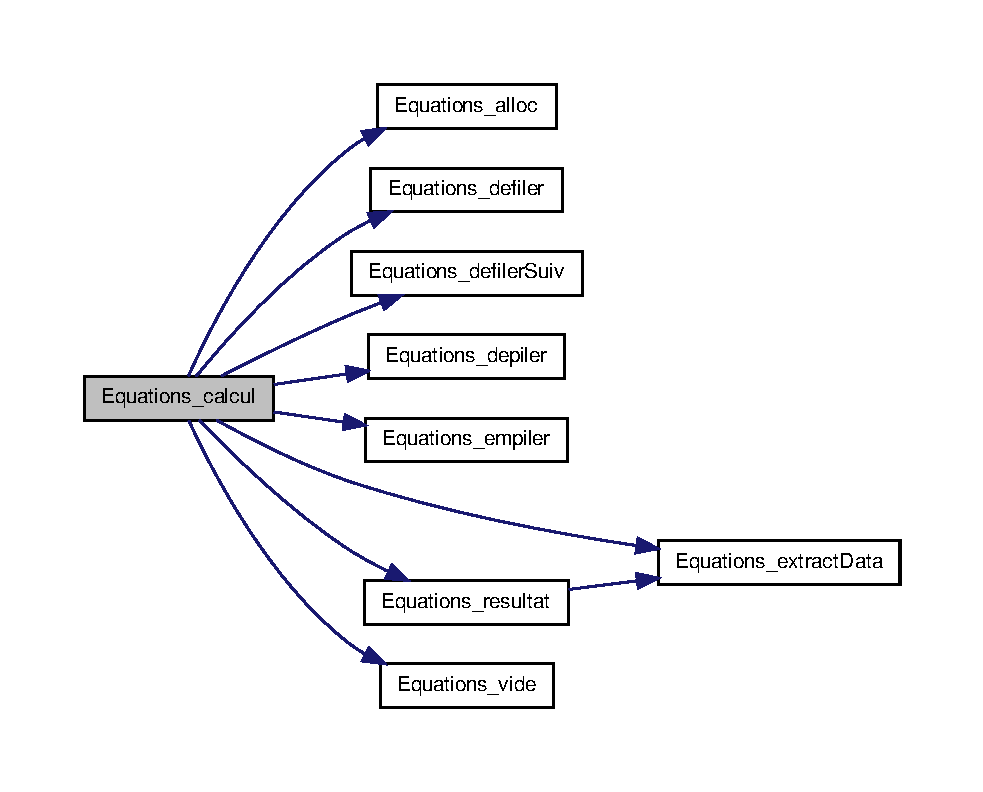
\includegraphics[width=400pt]{equations_8h_a6e6af023dd85b15e2af2129a5c857238_cgraph}
\end{center}
\end{figure}


\hypertarget{equations_8h_a7b5cc03bbac246e28d61714dc2931a92}{
\index{equations.h@{equations.h}!Equations\_\-defiler@{Equations\_\-defiler}}
\index{Equations\_\-defiler@{Equations\_\-defiler}!equations.h@{equations.h}}
\subsubsection[{Equations\_\-defiler}]{\setlength{\rightskip}{0pt plus 5cm}{\bf pEquations} Equations\_\-defiler (
\begin{DoxyParamCaption}
\item[{{\bf pEquations}}]{liste}
\end{DoxyParamCaption}
)}}
\label{equations_8h_a7b5cc03bbac246e28d61714dc2931a92}


Look for the first element of the struct \hyperlink{structEquations}{Equations}. 

\begin{DoxyAuthor}{Author}
Amine Ghozlane 
\end{DoxyAuthor}

\begin{DoxyParams}{Parameters}
{\em liste} & Struct \hyperlink{structEquations}{Equations} \\
\hline
\end{DoxyParams}
\begin{DoxyReturn}{Returns}
Pointer on the first element of struct \hyperlink{structEquations}{Equations} 
\end{DoxyReturn}


Definition at line 320 of file equations.c.



Referenced by Equations\_\-calcul(), and Equations\_\-emptyOp().

\hypertarget{equations_8h_a2c6acfd549462cb3be5a53775767429a}{
\index{equations.h@{equations.h}!Equations\_\-defilerSuiv@{Equations\_\-defilerSuiv}}
\index{Equations\_\-defilerSuiv@{Equations\_\-defilerSuiv}!equations.h@{equations.h}}
\subsubsection[{Equations\_\-defilerSuiv}]{\setlength{\rightskip}{0pt plus 5cm}{\bf pEquations} Equations\_\-defilerSuiv (
\begin{DoxyParamCaption}
\item[{{\bf pEquations}}]{liste}
\end{DoxyParamCaption}
)}}
\label{equations_8h_a2c6acfd549462cb3be5a53775767429a}


Get the next element of the struct \hyperlink{structEquations}{Equations}. 

\begin{DoxyAuthor}{Author}
Amine Ghozlane 
\end{DoxyAuthor}

\begin{DoxyParams}{Parameters}
{\em liste} & Struct \hyperlink{structEquations}{Equations} \\
\hline
\end{DoxyParams}
\begin{DoxyReturn}{Returns}
Pointer on the next element of struct \hyperlink{structEquations}{Equations} 
\end{DoxyReturn}


Definition at line 334 of file equations.c.



Referenced by Equations\_\-calcul(), and Equations\_\-emptyOp().

\hypertarget{equations_8h_afa3dcf131c38609646bd0ff79aef41d7}{
\index{equations.h@{equations.h}!Equations\_\-define@{Equations\_\-define}}
\index{Equations\_\-define@{Equations\_\-define}!equations.h@{equations.h}}
\subsubsection[{Equations\_\-define}]{\setlength{\rightskip}{0pt plus 5cm}void Equations\_\-define (
\begin{DoxyParamCaption}
\item[{{\bf pEquations}}]{new, }
\item[{char $\ast$}]{operateur}
\end{DoxyParamCaption}
)}}
\label{equations_8h_afa3dcf131c38609646bd0ff79aef41d7}


Identify the mathematical operator used. 

\begin{DoxyAuthor}{Author}
Amine Ghozlane 
\end{DoxyAuthor}

\begin{DoxyParams}{Parameters}
{\em new} & Struct \hyperlink{structEquations}{Equations} \\
\hline
{\em operateur} & Read operator \\
\hline
\end{DoxyParams}


Definition at line 174 of file equations.c.



References add(), addition, divide(), division, equal, equality(), inf(), inf\_\-equal(), inferior, inferior\_\-equal, multiplication, multiply(), soustraction, subtract(), sup(), sup\_\-equal(), superior, and superior\_\-equal.



Referenced by Equations\_\-pileFormation().



Here is the call graph for this function:\nopagebreak
\begin{figure}[H]
\begin{center}
\leavevmode
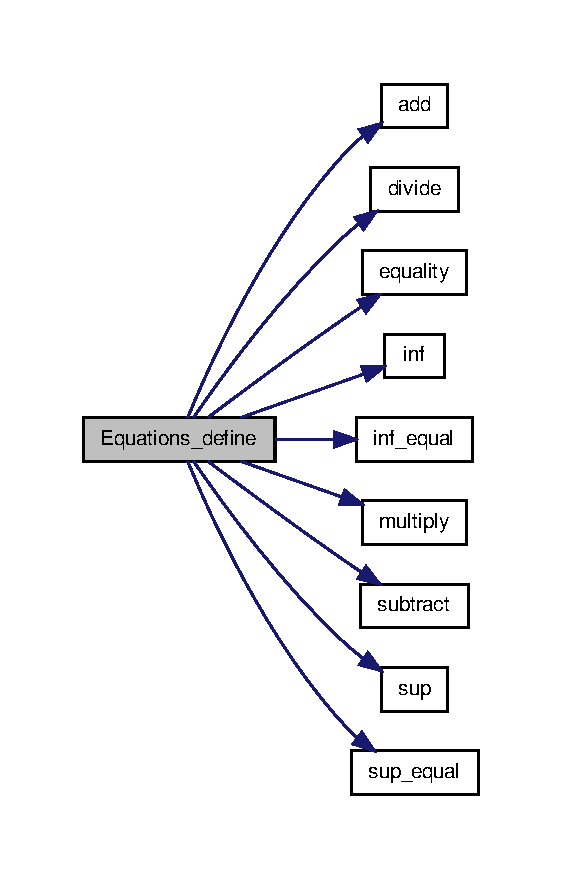
\includegraphics[width=270pt]{equations_8h_afa3dcf131c38609646bd0ff79aef41d7_cgraph}
\end{center}
\end{figure}


\hypertarget{equations_8h_ae69932ae59f7f39d19b16efdcd0ba814}{
\index{equations.h@{equations.h}!Equations\_\-depiler@{Equations\_\-depiler}}
\index{Equations\_\-depiler@{Equations\_\-depiler}!equations.h@{equations.h}}
\subsubsection[{Equations\_\-depiler}]{\setlength{\rightskip}{0pt plus 5cm}{\bf pEquations} Equations\_\-depiler (
\begin{DoxyParamCaption}
\item[{{\bf pEquations}}]{liste}
\end{DoxyParamCaption}
)}}
\label{equations_8h_ae69932ae59f7f39d19b16efdcd0ba814}


Unstack the last element of the struct \hyperlink{structEquations}{Equations}. 

\begin{DoxyAuthor}{Author}
Amine Ghozlane 
\end{DoxyAuthor}

\begin{DoxyParams}{Parameters}
{\em liste} & Struct \hyperlink{structEquations}{Equations}. \\
\hline
\end{DoxyParams}
\begin{DoxyReturn}{Returns}
Pointer on the \char`\"{}unstack\char`\"{} element of struct \hyperlink{structEquations}{Equations}. 
\end{DoxyReturn}


Definition at line 282 of file equations.c.



Referenced by Equations\_\-addOp(), and Equations\_\-calcul().

\hypertarget{equations_8h_ab8d4e4c2f309e68abe8dbcae96a240d5}{
\index{equations.h@{equations.h}!Equations\_\-empiler@{Equations\_\-empiler}}
\index{Equations\_\-empiler@{Equations\_\-empiler}!equations.h@{equations.h}}
\subsubsection[{Equations\_\-empiler}]{\setlength{\rightskip}{0pt plus 5cm}{\bf pEquations} Equations\_\-empiler (
\begin{DoxyParamCaption}
\item[{{\bf pEquations}}]{liste, }
\item[{{\bf pEquations}}]{new}
\end{DoxyParamCaption}
)}}
\label{equations_8h_ab8d4e4c2f309e68abe8dbcae96a240d5}


Stack an element to the struct \hyperlink{structEquations}{Equations}. 

\begin{DoxyAuthor}{Author}
Amine Ghozlane 
\end{DoxyAuthor}

\begin{DoxyParams}{Parameters}
{\em liste} & Struct \hyperlink{structEquations}{Equations} \\
\hline
{\em new} & New struct \hyperlink{structEquations}{Equations} element \\
\hline
\end{DoxyParams}
\begin{DoxyReturn}{Returns}
Pointer on the last element of struct \hyperlink{structEquations}{Equations} 
\end{DoxyReturn}


Definition at line 258 of file equations.c.



Referenced by Equations\_\-addOp(), Equations\_\-calcul(), Equations\_\-emptyOp(), and Equations\_\-pileFormation().

\hypertarget{equations_8h_ae188053c785ea42afda7a9a604140b44}{
\index{equations.h@{equations.h}!Equations\_\-emptyOp@{Equations\_\-emptyOp}}
\index{Equations\_\-emptyOp@{Equations\_\-emptyOp}!equations.h@{equations.h}}
\subsubsection[{Equations\_\-emptyOp}]{\setlength{\rightskip}{0pt plus 5cm}void Equations\_\-emptyOp (
\begin{DoxyParamCaption}
\item[{{\bf pEquations}}]{result, }
\item[{{\bf pEquations}}]{op}
\end{DoxyParamCaption}
)}}
\label{equations_8h_ae188053c785ea42afda7a9a604140b44}


Empty the Struct \hyperlink{structEquations}{Equations} op for the struct Equation result. 

\begin{DoxyAuthor}{Author}
Amine Ghozlane 
\end{DoxyAuthor}

\begin{DoxyParams}{Parameters}
{\em result} & Struct \hyperlink{structEquations}{Equations} used for computation \\
\hline
{\em op} & Struct Equation used to store the operator \\
\hline
\end{DoxyParams}


Definition at line 421 of file equations.c.



References Equations\_\-defiler(), Equations\_\-defilerSuiv(), Equations\_\-empiler(), and Equations\_\-vide().



Referenced by Equations\_\-pileFormation().



Here is the call graph for this function:\nopagebreak
\begin{figure}[H]
\begin{center}
\leavevmode
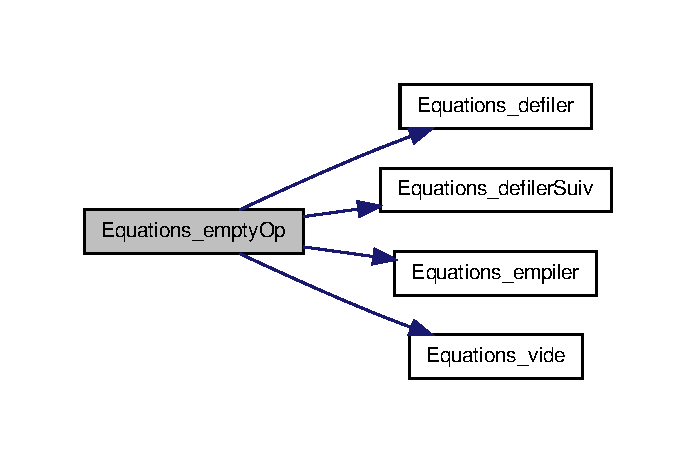
\includegraphics[width=334pt]{equations_8h_ae188053c785ea42afda7a9a604140b44_cgraph}
\end{center}
\end{figure}


\hypertarget{equations_8h_a543044646be5d2086c3301f7db2a0c1f}{
\index{equations.h@{equations.h}!Equations\_\-finalQuantite@{Equations\_\-finalQuantite}}
\index{Equations\_\-finalQuantite@{Equations\_\-finalQuantite}!equations.h@{equations.h}}
\subsubsection[{Equations\_\-finalQuantite}]{\setlength{\rightskip}{0pt plus 5cm}double Equations\_\-finalQuantite (
\begin{DoxyParamCaption}
\item[{int}]{file\_\-nb\_\-especes, }
\item[{char $\ast$$\ast$}]{file\_\-species, }
\item[{int $\ast$}]{file\_\-amount, }
\item[{int $\ast$}]{file\_\-weight, }
\item[{char $\ast$$\ast$}]{sim\_\-name, }
\item[{double $\ast$}]{sim\_\-quantite, }
\item[{int}]{sim\_\-taille}
\end{DoxyParamCaption}
)}}
\label{equations_8h_a543044646be5d2086c3301f7db2a0c1f}


Compute the score of the quantity which means the difference between what is expected to what is simulated. 

\begin{DoxyAuthor}{Author}
Amine Ghozlane 
\end{DoxyAuthor}

\begin{DoxyParams}{Parameters}
{\em file\_\-nb\_\-especes} & Number of species in the parameter file \\
\hline
{\em file\_\-species} & List of species in the parameter file \\
\hline
{\em file\_\-amount} & List of species expected quantity \\
\hline
{\em file\_\-weight} & Weight defined for the species \\
\hline
{\em sim\_\-name} & List of species simulated (sbml file) \\
\hline
{\em sim\_\-quantite} & List of the quantity of the species simulated (sbml file) \\
\hline
{\em sim\_\-taille} & Number of species simulated (sbml file) \\
\hline
\end{DoxyParams}
\begin{DoxyReturn}{Returns}
Result of the difference (Second part of the Energy) 
\end{DoxyReturn}


Definition at line 683 of file equations.c.



References Equations\_\-findSpecies().



Referenced by Min\_\-my\_\-f(), Mod\_\-compute\_\-modeling(), Recuit\_\-energyFunction(), and Sd\_\-compute\_\-simulation().



Here is the call graph for this function:\nopagebreak
\begin{figure}[H]
\begin{center}
\leavevmode
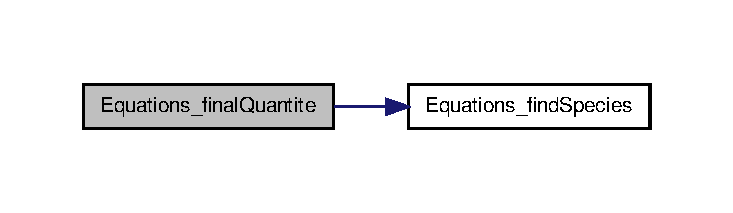
\includegraphics[width=352pt]{equations_8h_a543044646be5d2086c3301f7db2a0c1f_cgraph}
\end{center}
\end{figure}


\hypertarget{equations_8h_acacabe612b4e956d3db6d1677dac4037}{
\index{equations.h@{equations.h}!Equations\_\-findSpecies@{Equations\_\-findSpecies}}
\index{Equations\_\-findSpecies@{Equations\_\-findSpecies}!equations.h@{equations.h}}
\subsubsection[{Equations\_\-findSpecies}]{\setlength{\rightskip}{0pt plus 5cm}double Equations\_\-findSpecies (
\begin{DoxyParamCaption}
\item[{char $\ast$}]{species, }
\item[{char $\ast$$\ast$}]{name, }
\item[{double $\ast$}]{quantite, }
\item[{int}]{taille}
\end{DoxyParamCaption}
)}}
\label{equations_8h_acacabe612b4e956d3db6d1677dac4037}


Look for the quantity of a molecule in the list. 

\begin{DoxyAuthor}{Author}
Amine Ghozlane 
\end{DoxyAuthor}

\begin{DoxyParams}{Parameters}
{\em species} & Name of a molecule \\
\hline
{\em name} & List of molecules \\
\hline
{\em quantite} & List of the quantity of the molecules \\
\hline
{\em taille} & Number of molecules in the list \\
\hline
\end{DoxyParams}
\begin{DoxyReturn}{Returns}
Quantity of the molecule of interest 
\end{DoxyReturn}


Definition at line 533 of file equations.c.



Referenced by Equations\_\-finalQuantite(), Min\_\-score\_\-print\_\-mean(), and Mod\_\-score\_\-print\_\-mean().

\hypertarget{equations_8h_ae0f5b302dbd7d0bb1524b48aa38bec6c}{
\index{equations.h@{equations.h}!Equations\_\-pileFormation@{Equations\_\-pileFormation}}
\index{Equations\_\-pileFormation@{Equations\_\-pileFormation}!equations.h@{equations.h}}
\subsubsection[{Equations\_\-pileFormation}]{\setlength{\rightskip}{0pt plus 5cm}{\bf pEquations} Equations\_\-pileFormation (
\begin{DoxyParamCaption}
\item[{char $\ast$$\ast$$\ast$}]{equation, }
\item[{int}]{nb\_\-noeud}
\end{DoxyParamCaption}
)}}
\label{equations_8h_ae0f5b302dbd7d0bb1524b48aa38bec6c}


Build pile. 

\begin{DoxyAuthor}{Author}
Amine Ghozlane 
\end{DoxyAuthor}

\begin{DoxyParams}{Parameters}
{\em equation} & Table with the equation in Mathml format \\
\hline
{\em nb\_\-noeud} & Number of element inside the equation \\
\hline
\end{DoxyParams}
\begin{DoxyReturn}{Returns}
Struct Equation needed for compute the equation 
\end{DoxyReturn}


Definition at line 441 of file equations.c.



References constant, Equations\_\-addOp(), Equations\_\-alloc(), Equations\_\-define(), Equations\_\-empiler(), Equations\_\-emptyOp(), and variable.



Referenced by Data\_\-equationsInit().



Here is the call graph for this function:\nopagebreak
\begin{figure}[H]
\begin{center}
\leavevmode
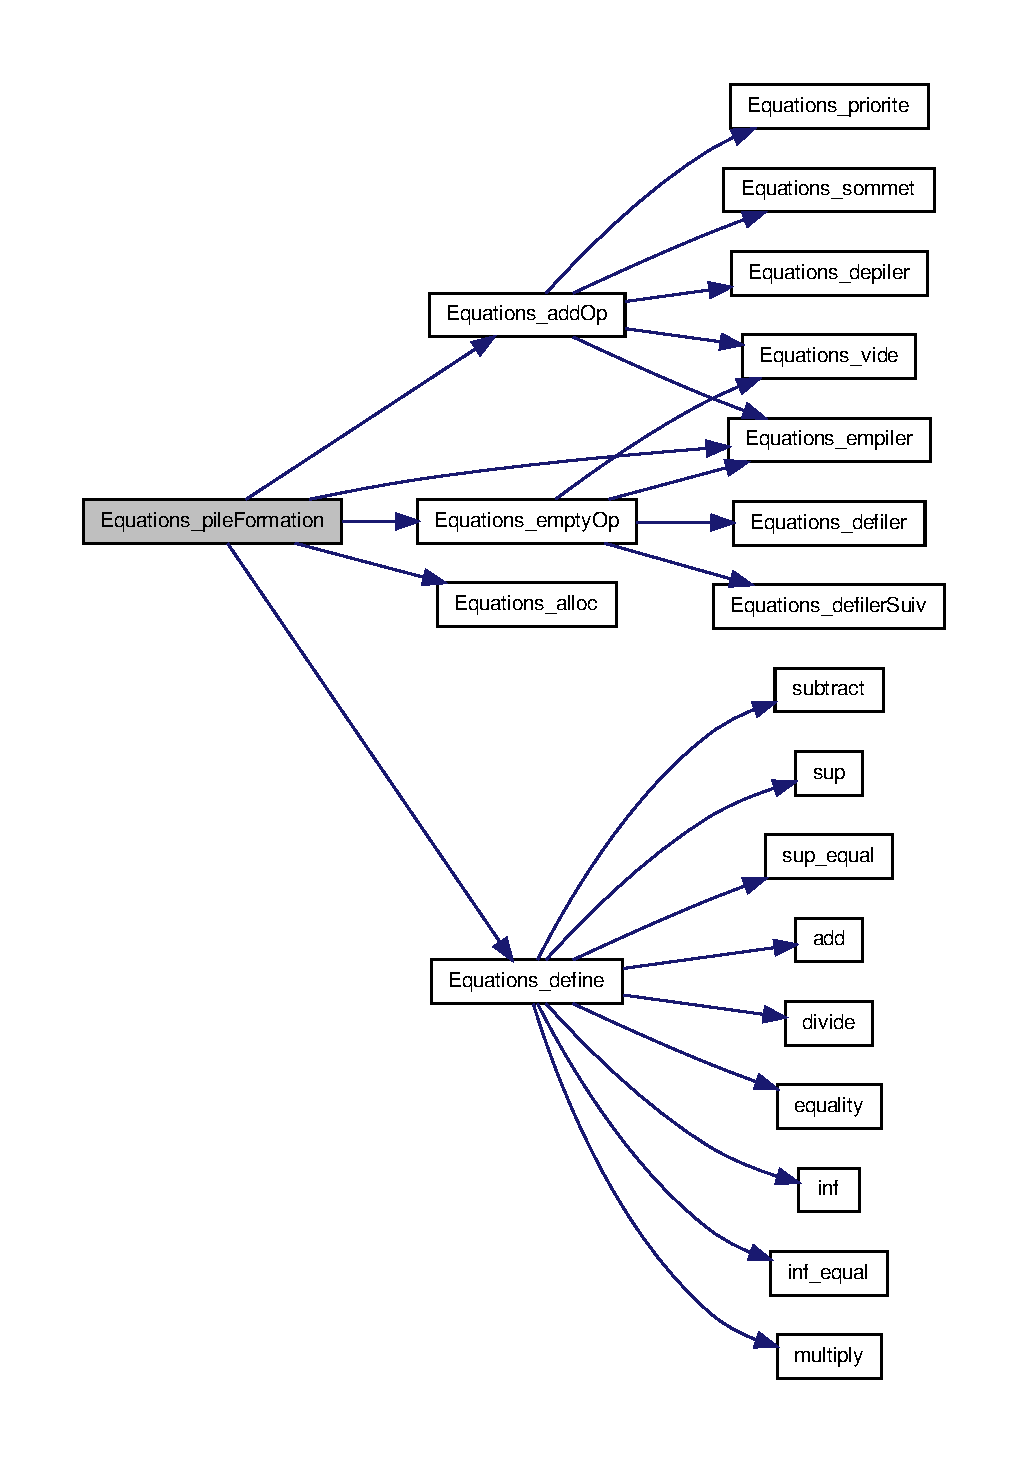
\includegraphics[width=400pt]{equations_8h_ae0f5b302dbd7d0bb1524b48aa38bec6c_cgraph}
\end{center}
\end{figure}


\hypertarget{equations_8h_ab5545fa4c945c64285e91687d90767f4}{
\index{equations.h@{equations.h}!Equations\_\-print@{Equations\_\-print}}
\index{Equations\_\-print@{Equations\_\-print}!equations.h@{equations.h}}
\subsubsection[{Equations\_\-print}]{\setlength{\rightskip}{0pt plus 5cm}void Equations\_\-print (
\begin{DoxyParamCaption}
\item[{{\bf pEquations}}]{liste}
\end{DoxyParamCaption}
)}}
\label{equations_8h_ab5545fa4c945c64285e91687d90767f4}


Print all information on the element of the struct \hyperlink{structEquations}{Equations}. 

\begin{DoxyAuthor}{Author}
Amine Ghozlane 
\end{DoxyAuthor}

\begin{DoxyParams}{Parameters}
{\em liste} & Struct \hyperlink{structEquations}{Equations} \\
\hline
\end{DoxyParams}


Definition at line 359 of file equations.c.



References constant, Equdata::data, Equations::info, Equations::type, Equdata::var, and variable.

\hypertarget{equations_8h_a9107be336f525ee8ee8bb0d56bc91d8b}{
\index{equations.h@{equations.h}!Equations\_\-priorite@{Equations\_\-priorite}}
\index{Equations\_\-priorite@{Equations\_\-priorite}!equations.h@{equations.h}}
\subsubsection[{Equations\_\-priorite}]{\setlength{\rightskip}{0pt plus 5cm}int Equations\_\-priorite (
\begin{DoxyParamCaption}
\item[{{\bf pEquations}}]{new}
\end{DoxyParamCaption}
)}}
\label{equations_8h_a9107be336f525ee8ee8bb0d56bc91d8b}


Give the priority of the operator. Multiplication and Division have higher priority than addition or subtration... 

\begin{DoxyAuthor}{Author}
Amine Ghozlane 
\end{DoxyAuthor}

\begin{DoxyParams}{Parameters}
{\em new} & One element of the struct \hyperlink{structEquations}{Equations} \\
\hline
\end{DoxyParams}
\begin{DoxyReturn}{Returns}
Priority of the operator 
\end{DoxyReturn}


Definition at line 346 of file equations.c.



References addition, equal, inferior, inferior\_\-equal, soustraction, superior, and superior\_\-equal.



Referenced by Equations\_\-addOp().

\hypertarget{equations_8h_af09f4513d82b106e8e9157f30c909529}{
\index{equations.h@{equations.h}!Equations\_\-resultat@{Equations\_\-resultat}}
\index{Equations\_\-resultat@{Equations\_\-resultat}!equations.h@{equations.h}}
\subsubsection[{Equations\_\-resultat}]{\setlength{\rightskip}{0pt plus 5cm}double Equations\_\-resultat (
\begin{DoxyParamCaption}
\item[{{\bf pEquations}}]{result, }
\item[{{\bf pEquations}}]{result1, }
\item[{{\bf pEquations}}]{eq, }
\item[{char $\ast$$\ast$}]{name, }
\item[{double $\ast$}]{quantite, }
\item[{int}]{taille}
\end{DoxyParamCaption}
)}}
\label{equations_8h_af09f4513d82b106e8e9157f30c909529}


Compute the result of two pile. 

\begin{DoxyAuthor}{Author}
Amine Ghozlane 
\end{DoxyAuthor}

\begin{DoxyParams}{Parameters}
{\em result} & Struct Equation result \\
\hline
{\em result1} & Struct Equation result after the operator \\
\hline
{\em eq} & Operator \\
\hline
{\em name} & List of molecules \\
\hline
{\em quantite} & List of the quantity of the molecules \\
\hline
{\em taille} & Number of molecules in the list \\
\hline
\end{DoxyParams}
\begin{DoxyReturn}{Returns}
Result of the two pile 
\end{DoxyReturn}


Definition at line 561 of file equations.c.



References equal, Equations\_\-extractData(), inferior, inferior\_\-equal, superior, superior\_\-equal, and Equations::type.



Referenced by Equations\_\-calcul().



Here is the call graph for this function:\nopagebreak
\begin{figure}[H]
\begin{center}
\leavevmode
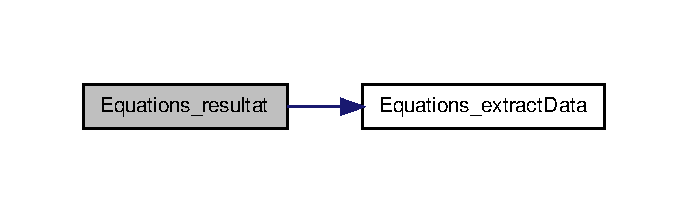
\includegraphics[width=330pt]{equations_8h_af09f4513d82b106e8e9157f30c909529_cgraph}
\end{center}
\end{figure}


\hypertarget{equations_8h_a25cc9b41f25936e9d67a650554dc875d}{
\index{equations.h@{equations.h}!Equations\_\-sommet@{Equations\_\-sommet}}
\index{Equations\_\-sommet@{Equations\_\-sommet}!equations.h@{equations.h}}
\subsubsection[{Equations\_\-sommet}]{\setlength{\rightskip}{0pt plus 5cm}{\bf pEquations} Equations\_\-sommet (
\begin{DoxyParamCaption}
\item[{{\bf pEquations}}]{liste}
\end{DoxyParamCaption}
)}}
\label{equations_8h_a25cc9b41f25936e9d67a650554dc875d}


Look for the last element of the struct \hyperlink{structEquations}{Equations}. 

\begin{DoxyAuthor}{Author}
Amine Ghozlane 
\end{DoxyAuthor}

\begin{DoxyParams}{Parameters}
{\em liste} & Struct \hyperlink{structEquations}{Equations} \\
\hline
\end{DoxyParams}
\begin{DoxyReturn}{Returns}
Pointer on the last element of struct \hyperlink{structEquations}{Equations} 
\end{DoxyReturn}


Definition at line 305 of file equations.c.



Referenced by Equations\_\-addOp().

\hypertarget{equations_8h_a7aa0efc05d71c770b8aaf4ad6d677be2}{
\index{equations.h@{equations.h}!Equations\_\-vide@{Equations\_\-vide}}
\index{Equations\_\-vide@{Equations\_\-vide}!equations.h@{equations.h}}
\subsubsection[{Equations\_\-vide}]{\setlength{\rightskip}{0pt plus 5cm}int Equations\_\-vide (
\begin{DoxyParamCaption}
\item[{{\bf pEquations}}]{liste}
\end{DoxyParamCaption}
)}}
\label{equations_8h_a7aa0efc05d71c770b8aaf4ad6d677be2}


Test if the struct \hyperlink{structEquations}{Equations} is empty. 

\begin{DoxyAuthor}{Author}
Amine Ghozlane 
\end{DoxyAuthor}

\begin{DoxyParams}{Parameters}
{\em liste} & Struct \hyperlink{structEquations}{Equations} \\
\hline
\end{DoxyParams}
\begin{DoxyReturn}{Returns}
Number of elements 
\end{DoxyReturn}


Definition at line 237 of file equations.c.



Referenced by Equations\_\-addOp(), Equations\_\-calcul(), and Equations\_\-emptyOp().

\hypertarget{equations_8h_a3a5c2f0eec28c21db099d689bbcc5b14}{
\index{equations.h@{equations.h}!inf@{inf}}
\index{inf@{inf}!equations.h@{equations.h}}
\subsubsection[{inf}]{\setlength{\rightskip}{0pt plus 5cm}double inf (
\begin{DoxyParamCaption}
\item[{double}]{arg1, }
\item[{double}]{arg2}
\end{DoxyParamCaption}
)}}
\label{equations_8h_a3a5c2f0eec28c21db099d689bbcc5b14}


Test the inferiority between two numbers. 

\begin{DoxyAuthor}{Author}
Amine Ghozlane 
\end{DoxyAuthor}

\begin{DoxyParams}{Parameters}
{\em arg1} & Value 1 \\
\hline
{\em arg2} & Value 2 \\
\hline
\end{DoxyParams}
\begin{DoxyReturn}{Returns}
Result 
\end{DoxyReturn}


Definition at line 134 of file equations.c.



Referenced by Equations\_\-define().

\hypertarget{equations_8h_aa6c076aacdfbdd13d6f25e0f36d6406b}{
\index{equations.h@{equations.h}!inf\_\-equal@{inf\_\-equal}}
\index{inf\_\-equal@{inf\_\-equal}!equations.h@{equations.h}}
\subsubsection[{inf\_\-equal}]{\setlength{\rightskip}{0pt plus 5cm}double inf\_\-equal (
\begin{DoxyParamCaption}
\item[{double}]{arg1, }
\item[{double}]{arg2}
\end{DoxyParamCaption}
)}}
\label{equations_8h_aa6c076aacdfbdd13d6f25e0f36d6406b}


Test the inferiority or equality between two numbers. 

\begin{DoxyAuthor}{Author}
Amine Ghozlane 
\end{DoxyAuthor}

\begin{DoxyParams}{Parameters}
{\em arg1} & Value 1 \\
\hline
{\em arg2} & Value 2 \\
\hline
\end{DoxyParams}
\begin{DoxyReturn}{Returns}
Result 
\end{DoxyReturn}


Definition at line 147 of file equations.c.



Referenced by Equations\_\-define().

\hypertarget{equations_8h_a6081051f0fa134ecbd577740cbb92220}{
\index{equations.h@{equations.h}!multiply@{multiply}}
\index{multiply@{multiply}!equations.h@{equations.h}}
\subsubsection[{multiply}]{\setlength{\rightskip}{0pt plus 5cm}double multiply (
\begin{DoxyParamCaption}
\item[{double}]{arg1, }
\item[{double}]{arg2}
\end{DoxyParamCaption}
)}}
\label{equations_8h_a6081051f0fa134ecbd577740cbb92220}


Multiply two numbers. 

\begin{DoxyAuthor}{Author}
Amine Ghozlane 
\end{DoxyAuthor}

\begin{DoxyParams}{Parameters}
{\em arg1} & Value 1 \\
\hline
{\em arg2} & Value 2 \\
\hline
\end{DoxyParams}
\begin{DoxyReturn}{Returns}
Result 
\end{DoxyReturn}


Definition at line 69 of file equations.c.



Referenced by Equations\_\-define().

\hypertarget{equations_8h_a8c90ae25e75adcfeeaf307cc2df2f360}{
\index{equations.h@{equations.h}!subtract@{subtract}}
\index{subtract@{subtract}!equations.h@{equations.h}}
\subsubsection[{subtract}]{\setlength{\rightskip}{0pt plus 5cm}double subtract (
\begin{DoxyParamCaption}
\item[{double}]{arg1, }
\item[{double}]{arg2}
\end{DoxyParamCaption}
)}}
\label{equations_8h_a8c90ae25e75adcfeeaf307cc2df2f360}


Subtraction two numbers. 

\begin{DoxyAuthor}{Author}
Amine Ghozlane 
\end{DoxyAuthor}

\begin{DoxyParams}{Parameters}
{\em arg1} & Value 1 \\
\hline
{\em arg2} & Value 2 \\
\hline
\end{DoxyParams}
\begin{DoxyReturn}{Returns}
Result 
\end{DoxyReturn}


Definition at line 56 of file equations.c.



Referenced by Equations\_\-define().

\hypertarget{equations_8h_a0ce3f625ded68dd2b0a927b1c3d85471}{
\index{equations.h@{equations.h}!sup@{sup}}
\index{sup@{sup}!equations.h@{equations.h}}
\subsubsection[{sup}]{\setlength{\rightskip}{0pt plus 5cm}double sup (
\begin{DoxyParamCaption}
\item[{double}]{arg1, }
\item[{double}]{arg2}
\end{DoxyParamCaption}
)}}
\label{equations_8h_a0ce3f625ded68dd2b0a927b1c3d85471}


Test the superiority between two numbers. 

\begin{DoxyAuthor}{Author}
Amine Ghozlane 
\end{DoxyAuthor}

\begin{DoxyParams}{Parameters}
{\em arg1} & Value 1 \\
\hline
{\em arg2} & Value 2 \\
\hline
\end{DoxyParams}
\begin{DoxyReturn}{Returns}
Result 
\end{DoxyReturn}


Definition at line 108 of file equations.c.



Referenced by Equations\_\-define().

\hypertarget{equations_8h_a26bbff8f2c38ba14fea7a9d6067329b2}{
\index{equations.h@{equations.h}!sup\_\-equal@{sup\_\-equal}}
\index{sup\_\-equal@{sup\_\-equal}!equations.h@{equations.h}}
\subsubsection[{sup\_\-equal}]{\setlength{\rightskip}{0pt plus 5cm}double sup\_\-equal (
\begin{DoxyParamCaption}
\item[{double}]{arg1, }
\item[{double}]{arg2}
\end{DoxyParamCaption}
)}}
\label{equations_8h_a26bbff8f2c38ba14fea7a9d6067329b2}


Test the superiority or equality between two numbers. 

\begin{DoxyAuthor}{Author}
Amine Ghozlane 
\end{DoxyAuthor}

\begin{DoxyParams}{Parameters}
{\em arg1} & Value 1 \\
\hline
{\em arg2} & Value 2 \\
\hline
\end{DoxyParams}
\begin{DoxyReturn}{Returns}
Result 
\end{DoxyReturn}


Definition at line 121 of file equations.c.



Referenced by Equations\_\-define().


\hypertarget{especes_8h}{
\section{metaboflux/include/especes.h File Reference}
\label{especes_8h}\index{metaboflux/include/especes.h@{metaboflux/include/especes.h}}
}


Modelize a molecule.  


This graph shows which files directly or indirectly include this file:\nopagebreak
\begin{figure}[H]
\begin{center}
\leavevmode
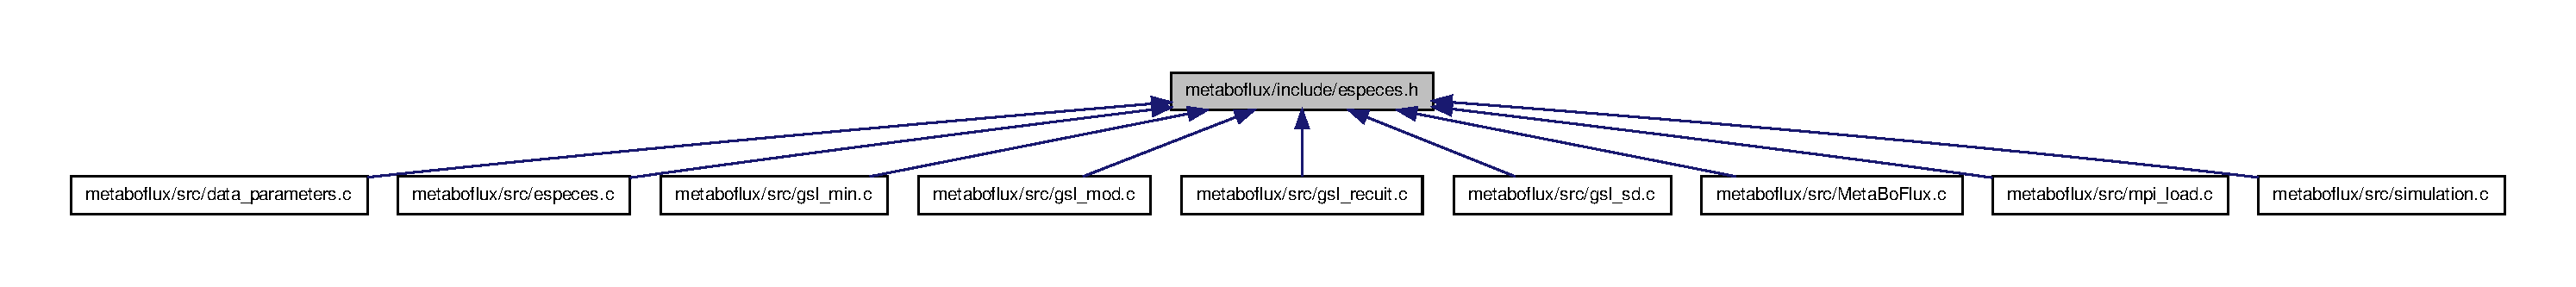
\includegraphics[width=400pt]{especes_8h__dep__incl}
\end{center}
\end{figure}
\subsection*{Data Structures}
\begin{DoxyCompactItemize}
\item 
struct \hyperlink{structReaction}{Reaction}
\begin{DoxyCompactList}\small\item\em Reactions data. \end{DoxyCompactList}\item 
struct \hyperlink{structEspeces}{Especes}
\begin{DoxyCompactList}\small\item\em Molecules data. \end{DoxyCompactList}\end{DoxyCompactItemize}
\subsection*{Functions}
\begin{DoxyCompactItemize}
\item 
\hyperlink{structEspeces}{pEspeces} \hyperlink{especes_8h_a1610e9ef9702676f49dda6e338fc8ceb}{Especes\_\-alloc} (int)
\begin{DoxyCompactList}\small\item\em Alloc memory and initialize the struct \hyperlink{structEspeces}{Especes}. \end{DoxyCompactList}\item 
void \hyperlink{especes_8h_a622cfe5dc2bba2275a7316755ee08142}{Especes\_\-allocReactions} (\hyperlink{structEspeces}{pEspeces}, int, Reaction\_\-t $\ast$, double)
\begin{DoxyCompactList}\small\item\em Alloc memory and initialize the struct \hyperlink{structReaction}{Reaction} for each molecule. \end{DoxyCompactList}\item 
void \hyperlink{especes_8h_a4e81e01f1f8e3b472bfdc2ea0dd5b769}{Especes\_\-free} (\hyperlink{structEspeces}{pEspeces}, int)
\begin{DoxyCompactList}\small\item\em Free the struct pEspeces. \end{DoxyCompactList}\item 
void \hyperlink{especes_8h_a271e25633ee1c9081b1b8b46f441be04}{Especes\_\-freeReactions} (\hyperlink{structEspeces}{Especes})
\begin{DoxyCompactList}\small\item\em Free the struct \hyperlink{structReaction}{Reaction}. \end{DoxyCompactList}\item 
void \hyperlink{especes_8h_abb8810a8cb8bd51a12838f893e58e97b}{Especes\_\-save} (\hyperlink{structEspeces}{pEspeces}, int, double, const char $\ast$)
\begin{DoxyCompactList}\small\item\em Save data on one molecule. \end{DoxyCompactList}\item 
void \hyperlink{especes_8h_a7f7d4b4764b583179bebcc86bbba09ed}{Especes\_\-scoreSpecies} (\hyperlink{structEspeces}{pEspeces}, int, char $\ast$$\ast$, double $\ast$)
\begin{DoxyCompactList}\small\item\em Save the quantite of all molecules for scoring. \end{DoxyCompactList}\item 
void \hyperlink{especes_8h_a120630120d7c5a6cded061eab659048a}{Especes\_\-print} (\hyperlink{structEspeces}{pEspeces}, int)
\begin{DoxyCompactList}\small\item\em Print data on each molecule. \end{DoxyCompactList}\item 
void \hyperlink{especes_8h_ad534ec7af1733aaf00880570d5fc99b2}{Especes\_\-print\_\-2} (\hyperlink{structEspeces}{pEspeces} molecules, int nbEspeces)
\begin{DoxyCompactList}\small\item\em Print Id and quantity on each molecule. \end{DoxyCompactList}\item 
int \hyperlink{especes_8h_a321b94dc8b65a8ff167218edb83df25e}{Especes\_\-find} (\hyperlink{structEspeces}{pEspeces}, const char $\ast$, int)
\begin{DoxyCompactList}\small\item\em Find a molecule thank to it ID. \end{DoxyCompactList}\item 
void \hyperlink{especes_8h_acfdb089ad290ca7a4b3bc4c58957c1ac}{Especes\_\-setQuantite} (\hyperlink{structEspeces}{pEspeces}, int, double)
\begin{DoxyCompactList}\small\item\em Change the quantity of a molecule. \end{DoxyCompactList}\item 
double \hyperlink{especes_8h_a25fe0df8949f57735787b5a4e5cf5a3c}{Especes\_\-getQuantite} (\hyperlink{structEspeces}{pEspeces}, int)
\begin{DoxyCompactList}\small\item\em Get the quanty of one molecule by its number. \end{DoxyCompactList}\item 
int \hyperlink{especes_8h_a3391146ab0a83b7db9cbe3bdaec9fdab}{Especes\_\-getNbreactions} (\hyperlink{structEspeces}{pEspeces} molecules, int ref)
\begin{DoxyCompactList}\small\item\em Get number of reaction where one molecule is used (like a reactif) \end{DoxyCompactList}\end{DoxyCompactItemize}


\subsection{Detailed Description}
Modelize a molecule. This file is part of MetaBoFlux (\href{http://www.cbib.u-bordeaux2.fr/metaboflux/}{\tt http://www.cbib.u-\/bordeaux2.fr/metaboflux/}) Copyright (C) 2010 Amine Ghozlane from LaBRI and University of Bordeaux 1

MetaBoFlux is free software: you can redistribute it and/or modify it under the terms of the GNU Lesser General Public License as published by the Free Software Foundation, either version 3 of the License, or (at your option) any later version.

MetaBoFlux is distributed in the hope that it will be useful, but WITHOUT ANY WARRANTY; without even the implied warranty of MERCHANTABILITY or FITNESS FOR A PARTICULAR PURPOSE. See the GNU General Public License for more details.

You should have received a copy of the GNU Lesser General Public License along with this program. If not, see $<$\href{http://www.gnu.org/licenses/}{\tt http://www.gnu.org/licenses/}$>$.

\begin{DoxyAuthor}{Author}
\{Amine Ghozlane\} 
\end{DoxyAuthor}
\begin{DoxyVersion}{Version}
2.0 
\end{DoxyVersion}
\begin{DoxyDate}{Date}
27 octobre 2009 
\end{DoxyDate}


Definition in file \hyperlink{especes_8h_source}{especes.h}.



\subsection{Function Documentation}
\hypertarget{especes_8h_a1610e9ef9702676f49dda6e338fc8ceb}{
\index{especes.h@{especes.h}!Especes\_\-alloc@{Especes\_\-alloc}}
\index{Especes\_\-alloc@{Especes\_\-alloc}!especes.h@{especes.h}}
\subsubsection[{Especes\_\-alloc}]{\setlength{\rightskip}{0pt plus 5cm}{\bf pEspeces} Especes\_\-alloc (
\begin{DoxyParamCaption}
\item[{int}]{nbEspeces}
\end{DoxyParamCaption}
)}}
\label{especes_8h_a1610e9ef9702676f49dda6e338fc8ceb}


Alloc memory and initialize the struct \hyperlink{structEspeces}{Especes}. 

\begin{DoxyAuthor}{Author}
Amine Ghozlane 
\end{DoxyAuthor}

\begin{DoxyParams}{Parameters}
{\em nbEspeces} & Number of molecules \\
\hline
\end{DoxyParams}
\begin{DoxyReturn}{Returns}
Allocated struct Espece 
\end{DoxyReturn}


Definition at line 40 of file especes.c.



References Especes::quantite, and Especes::system.



Referenced by SBML\_\-compute\_\-simulation(), and SBML\_\-compute\_\-simulation\_\-mean().

\hypertarget{especes_8h_a622cfe5dc2bba2275a7316755ee08142}{
\index{especes.h@{especes.h}!Especes\_\-allocReactions@{Especes\_\-allocReactions}}
\index{Especes\_\-allocReactions@{Especes\_\-allocReactions}!especes.h@{especes.h}}
\subsubsection[{Especes\_\-allocReactions}]{\setlength{\rightskip}{0pt plus 5cm}void Especes\_\-allocReactions (
\begin{DoxyParamCaption}
\item[{{\bf pEspeces}}]{molecules, }
\item[{int}]{Espece, }
\item[{Reaction\_\-t $\ast$}]{local, }
\item[{double}]{reactRatio}
\end{DoxyParamCaption}
)}}
\label{especes_8h_a622cfe5dc2bba2275a7316755ee08142}


Alloc memory and initialize the struct \hyperlink{structReaction}{Reaction} for each molecule. 

\begin{DoxyAuthor}{Author}
Amine Ghozlane 
\end{DoxyAuthor}

\begin{DoxyParams}{Parameters}
{\em molecules} & List of molecules \\
\hline
{\em Espece} & Number of the selected molecule \\
\hline
{\em local} & \hyperlink{structReaction}{Reaction} sbml reference \\
\hline
{\em reactRatio} & Ratio of the reaction \\
\hline
\end{DoxyParams}


Definition at line 64 of file especes.c.



References Reaction::link, Reaction::suivant, and Especes::system.



Referenced by SBML\_\-setReactions().

\hypertarget{especes_8h_a321b94dc8b65a8ff167218edb83df25e}{
\index{especes.h@{especes.h}!Especes\_\-find@{Especes\_\-find}}
\index{Especes\_\-find@{Especes\_\-find}!especes.h@{especes.h}}
\subsubsection[{Especes\_\-find}]{\setlength{\rightskip}{0pt plus 5cm}int Especes\_\-find (
\begin{DoxyParamCaption}
\item[{{\bf pEspeces}}]{molecules, }
\item[{const char $\ast$}]{especeId, }
\item[{int}]{nbEspeces}
\end{DoxyParamCaption}
)}}
\label{especes_8h_a321b94dc8b65a8ff167218edb83df25e}


Find a molecule thank to it ID. 

\begin{DoxyAuthor}{Author}
Amine Ghozlane 
\end{DoxyAuthor}

\begin{DoxyParams}{Parameters}
{\em molecules} & List of molecules \\
\hline
{\em especeId} & SBML ID of the molecule \\
\hline
{\em nbEspeces} & Number of molecules \\
\hline
\end{DoxyParams}
\begin{DoxyReturn}{Returns}
Number of a selected molecule 
\end{DoxyReturn}


Definition at line 214 of file especes.c.



Referenced by SBML\_\-checkQuantite(), SBML\_\-reaction(), and SBML\_\-setReactions().

\hypertarget{especes_8h_a4e81e01f1f8e3b472bfdc2ea0dd5b769}{
\index{especes.h@{especes.h}!Especes\_\-free@{Especes\_\-free}}
\index{Especes\_\-free@{Especes\_\-free}!especes.h@{especes.h}}
\subsubsection[{Especes\_\-free}]{\setlength{\rightskip}{0pt plus 5cm}void Especes\_\-free (
\begin{DoxyParamCaption}
\item[{{\bf pEspeces}}]{molecules, }
\item[{int}]{nbEspeces}
\end{DoxyParamCaption}
)}}
\label{especes_8h_a4e81e01f1f8e3b472bfdc2ea0dd5b769}


Free the struct pEspeces. 

\begin{DoxyAuthor}{Author}
Amine Ghozlane 
\end{DoxyAuthor}

\begin{DoxyParams}{Parameters}
{\em molecules} & List of molecules \\
\hline
{\em nbEspeces} & Number of molecules \\
\hline
\end{DoxyParams}


Definition at line 94 of file especes.c.



References Especes\_\-freeReactions().



Referenced by SBML\_\-compute\_\-simulation(), and SBML\_\-compute\_\-simulation\_\-mean().



Here is the call graph for this function:\nopagebreak
\begin{figure}[H]
\begin{center}
\leavevmode
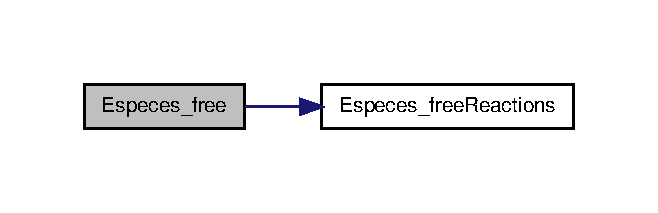
\includegraphics[width=316pt]{especes_8h_a4e81e01f1f8e3b472bfdc2ea0dd5b769_cgraph}
\end{center}
\end{figure}


\hypertarget{especes_8h_a271e25633ee1c9081b1b8b46f441be04}{
\index{especes.h@{especes.h}!Especes\_\-freeReactions@{Especes\_\-freeReactions}}
\index{Especes\_\-freeReactions@{Especes\_\-freeReactions}!especes.h@{especes.h}}
\subsubsection[{Especes\_\-freeReactions}]{\setlength{\rightskip}{0pt plus 5cm}void Especes\_\-freeReactions (
\begin{DoxyParamCaption}
\item[{{\bf Especes}}]{molecules}
\end{DoxyParamCaption}
)}}
\label{especes_8h_a271e25633ee1c9081b1b8b46f441be04}


Free the struct \hyperlink{structReaction}{Reaction}. 

\begin{DoxyAuthor}{Author}
Amine Ghozlane 
\end{DoxyAuthor}

\begin{DoxyParams}{Parameters}
{\em molecules} & List of molecules \\
\hline
\end{DoxyParams}


Definition at line 109 of file especes.c.



References Reaction::suivant, and Especes::system.



Referenced by Especes\_\-free().

\hypertarget{especes_8h_a3391146ab0a83b7db9cbe3bdaec9fdab}{
\index{especes.h@{especes.h}!Especes\_\-getNbreactions@{Especes\_\-getNbreactions}}
\index{Especes\_\-getNbreactions@{Especes\_\-getNbreactions}!especes.h@{especes.h}}
\subsubsection[{Especes\_\-getNbreactions}]{\setlength{\rightskip}{0pt plus 5cm}int Especes\_\-getNbreactions (
\begin{DoxyParamCaption}
\item[{{\bf pEspeces}}]{molecules, }
\item[{int}]{ref}
\end{DoxyParamCaption}
)}}
\label{especes_8h_a3391146ab0a83b7db9cbe3bdaec9fdab}


Get number of reaction where one molecule is used (like a reactif) 

\begin{DoxyAuthor}{Author}
Amine Ghozlane 
\end{DoxyAuthor}

\begin{DoxyParams}{Parameters}
{\em molecules} & List of molecules \\
\hline
{\em ref} & Number of a selected molecule \\
\hline
\end{DoxyParams}
\begin{DoxyReturn}{Returns}
Number of reactions 
\end{DoxyReturn}


Definition at line 265 of file especes.c.



References Reaction::suivant, and Especes::system.



Referenced by SBML\_\-simulate().

\hypertarget{especes_8h_a25fe0df8949f57735787b5a4e5cf5a3c}{
\index{especes.h@{especes.h}!Especes\_\-getQuantite@{Especes\_\-getQuantite}}
\index{Especes\_\-getQuantite@{Especes\_\-getQuantite}!especes.h@{especes.h}}
\subsubsection[{Especes\_\-getQuantite}]{\setlength{\rightskip}{0pt plus 5cm}double Especes\_\-getQuantite (
\begin{DoxyParamCaption}
\item[{{\bf pEspeces}}]{molecules, }
\item[{int}]{Especes}
\end{DoxyParamCaption}
)}}
\label{especes_8h_a25fe0df8949f57735787b5a4e5cf5a3c}


Get the quanty of one molecule by its number. 

\begin{DoxyAuthor}{Author}
Amine Ghozlane 
\end{DoxyAuthor}

\begin{DoxyParams}{Parameters}
{\em molecules} & List of molecules \\
\hline
{\em \hyperlink{structEspeces}{Especes}} & Number of a selected molecule \\
\hline
\end{DoxyParams}
\begin{DoxyReturn}{Returns}
Quantity of a selected molecule 
\end{DoxyReturn}


Definition at line 252 of file especes.c.



References Especes::quantite.



Referenced by SBML\_\-checkQuantite(), SBML\_\-reaction(), and SBML\_\-simulate().

\hypertarget{especes_8h_a120630120d7c5a6cded061eab659048a}{
\index{especes.h@{especes.h}!Especes\_\-print@{Especes\_\-print}}
\index{Especes\_\-print@{Especes\_\-print}!especes.h@{especes.h}}
\subsubsection[{Especes\_\-print}]{\setlength{\rightskip}{0pt plus 5cm}void Especes\_\-print (
\begin{DoxyParamCaption}
\item[{{\bf pEspeces}}]{molecules, }
\item[{int}]{nbEspeces}
\end{DoxyParamCaption}
)}}
\label{especes_8h_a120630120d7c5a6cded061eab659048a}


Print data on each molecule. 

\begin{DoxyAuthor}{Author}
Amine Ghozlane 
\end{DoxyAuthor}

\begin{DoxyParams}{Parameters}
{\em molecules} & List of molecules \\
\hline
{\em nbEspeces} & Number of molecules \\
\hline
\end{DoxyParams}


Definition at line 170 of file especes.c.



References Reaction::link, Reaction::suivant, and Especes::system.

\hypertarget{especes_8h_ad534ec7af1733aaf00880570d5fc99b2}{
\index{especes.h@{especes.h}!Especes\_\-print\_\-2@{Especes\_\-print\_\-2}}
\index{Especes\_\-print\_\-2@{Especes\_\-print\_\-2}!especes.h@{especes.h}}
\subsubsection[{Especes\_\-print\_\-2}]{\setlength{\rightskip}{0pt plus 5cm}void Especes\_\-print\_\-2 (
\begin{DoxyParamCaption}
\item[{{\bf pEspeces}}]{molecules, }
\item[{int}]{nbEspeces}
\end{DoxyParamCaption}
)}}
\label{especes_8h_ad534ec7af1733aaf00880570d5fc99b2}


Print Id and quantity on each molecule. 

\begin{DoxyAuthor}{Author}
Amine Ghozlane 
\end{DoxyAuthor}

\begin{DoxyParams}{Parameters}
{\em molecules} & List of molecules \\
\hline
{\em nbEspeces} & Number of molecules \\
\hline
\end{DoxyParams}


Definition at line 196 of file especes.c.

\hypertarget{especes_8h_abb8810a8cb8bd51a12838f893e58e97b}{
\index{especes.h@{especes.h}!Especes\_\-save@{Especes\_\-save}}
\index{Especes\_\-save@{Especes\_\-save}!especes.h@{especes.h}}
\subsubsection[{Especes\_\-save}]{\setlength{\rightskip}{0pt plus 5cm}void Especes\_\-save (
\begin{DoxyParamCaption}
\item[{{\bf pEspeces}}]{molecules, }
\item[{int}]{i, }
\item[{double}]{quant, }
\item[{const char $\ast$}]{dye}
\end{DoxyParamCaption}
)}}
\label{especes_8h_abb8810a8cb8bd51a12838f893e58e97b}


Save data on one molecule. 

\begin{DoxyAuthor}{Author}
Amine Ghozlane 
\end{DoxyAuthor}

\begin{DoxyParams}{Parameters}
{\em molecules} & List of molecules \\
\hline
{\em i} & Number of the selected molecule \\
\hline
{\em quant} & Quantity of the molecule \\
\hline
{\em dye} & ID of the molecule \\
\hline
\end{DoxyParams}


Definition at line 134 of file especes.c.



References Especes::id, and Especes::quantite.



Referenced by SBML\_\-initEspeceAmounts().

\hypertarget{especes_8h_a7f7d4b4764b583179bebcc86bbba09ed}{
\index{especes.h@{especes.h}!Especes\_\-scoreSpecies@{Especes\_\-scoreSpecies}}
\index{Especes\_\-scoreSpecies@{Especes\_\-scoreSpecies}!especes.h@{especes.h}}
\subsubsection[{Especes\_\-scoreSpecies}]{\setlength{\rightskip}{0pt plus 5cm}void Especes\_\-scoreSpecies (
\begin{DoxyParamCaption}
\item[{{\bf pEspeces}}]{molecules, }
\item[{int}]{nbEspeces, }
\item[{char $\ast$$\ast$}]{name, }
\item[{double $\ast$}]{quantite}
\end{DoxyParamCaption}
)}}
\label{especes_8h_a7f7d4b4764b583179bebcc86bbba09ed}


Save the quantite of all molecules for scoring. 

\begin{DoxyAuthor}{Author}
Amine Ghozlane 
\end{DoxyAuthor}

\begin{DoxyParams}{Parameters}
{\em molecules} & List of molecules \\
\hline
{\em nbEspeces} & Number of molecules \\
\hline
{\em name} & ID of the selected molecule \\
\hline
{\em quantite} & Table of molecule Quantity \\
\hline
\end{DoxyParams}


Definition at line 149 of file especes.c.



References Especes::quantite.



Referenced by SBML\_\-score().

\hypertarget{especes_8h_acfdb089ad290ca7a4b3bc4c58957c1ac}{
\index{especes.h@{especes.h}!Especes\_\-setQuantite@{Especes\_\-setQuantite}}
\index{Especes\_\-setQuantite@{Especes\_\-setQuantite}!especes.h@{especes.h}}
\subsubsection[{Especes\_\-setQuantite}]{\setlength{\rightskip}{0pt plus 5cm}void Especes\_\-setQuantite (
\begin{DoxyParamCaption}
\item[{{\bf pEspeces}}]{molecules, }
\item[{int}]{Especes, }
\item[{double}]{quant}
\end{DoxyParamCaption}
)}}
\label{especes_8h_acfdb089ad290ca7a4b3bc4c58957c1ac}


Change the quantity of a molecule. 

\begin{DoxyAuthor}{Author}
Amine Ghozlane 
\end{DoxyAuthor}

\begin{DoxyParams}{Parameters}
{\em molecules} & List of molecules \\
\hline
{\em \hyperlink{structEspeces}{Especes}} & Number of a selected molecule \\
\hline
{\em quant} & Quantity of the molecule \\
\hline
\end{DoxyParams}


Definition at line 239 of file especes.c.



References Especes::quantite.



Referenced by SBML\_\-reaction().


\hypertarget{gsl__min_8h}{
\section{metaboflux/include/gsl\_\-min.h File Reference}
\label{gsl__min_8h}\index{metaboflux/include/gsl\_\-min.h@{metaboflux/include/gsl\_\-min.h}}
}


Compute minimization of scenarii.  


This graph shows which files directly or indirectly include this file:\nopagebreak
\begin{figure}[H]
\begin{center}
\leavevmode
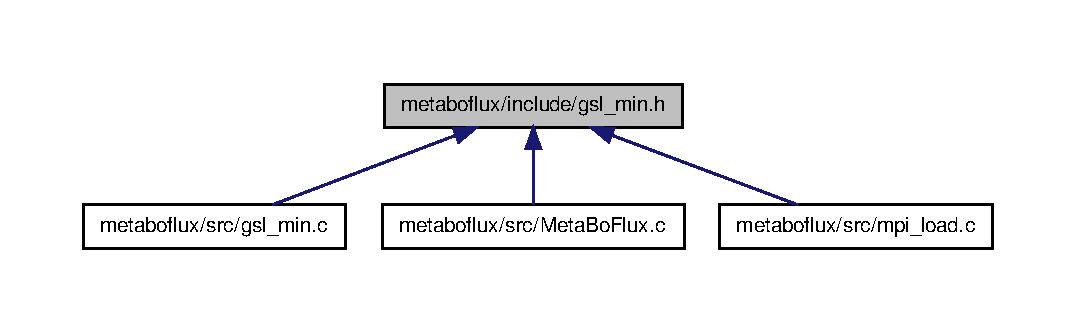
\includegraphics[width=400pt]{gsl__min_8h__dep__incl}
\end{center}
\end{figure}
\subsection*{Functions}
\begin{DoxyCompactItemize}
\item 
int \hyperlink{gsl__min_8h_a8d981de0373a06da9601e1b5eef379e1}{Min\_\-copieTab2} (double $\ast$, int, int, int)
\begin{DoxyCompactList}\small\item\em Copy table of reaction parameters. \end{DoxyCompactList}\item 
int \hyperlink{gsl__min_8h_a1f1d9c640473d18e2c9c092428d7052f}{Min\_\-copieTab3} (gsl\_\-multimin\_\-fminimizer $\ast$, int, int, int)
\begin{DoxyCompactList}\small\item\em Copy short table of parameter into the larger table. \end{DoxyCompactList}\item 
void \hyperlink{gsl__min_8h_a2d2f0b8fd130c026d88c29339e3766fa}{Min\_\-verifValue} (gsl\_\-vector $\ast$, double $\ast$, int, int)
\begin{DoxyCompactList}\small\item\em Checking reaction ratio parameters. \end{DoxyCompactList}\item 
double \hyperlink{gsl__min_8h_ac0cf1b97696b91752884777f11368223}{Min\_\-my\_\-f} (const gsl\_\-vector $\ast$, void $\ast$)
\begin{DoxyCompactList}\small\item\em Enter in the program for standard deviation. \end{DoxyCompactList}\item 
void \hyperlink{gsl__min_8h_a843d6e8ed1d3354a55586c7734f60499}{Min\_\-getTampon} (double $\ast$, double)
\begin{DoxyCompactList}\small\item\em Enter in the program for standard deviation. \end{DoxyCompactList}\item 
void \hyperlink{gsl__min_8h_a6fc9a31eec661815e3b5b83fc196d652}{Min\_\-score\_\-print\_\-mean} (double $\ast$)
\begin{DoxyCompactList}\small\item\em Save the minimization result. \end{DoxyCompactList}\item 
void \hyperlink{gsl__min_8h_a016be27ae853d4d14d48d81c626b1e50}{Min\_\-compute\_\-minimization} (\hyperlink{structListParameters}{pListParameters}, double $\ast$, double $\ast$, char $\ast$$\ast$, int, int)
\begin{DoxyCompactList}\small\item\em Compute the minimization. \end{DoxyCompactList}\end{DoxyCompactItemize}


\subsection{Detailed Description}
Compute minimization of scenarii. This file is part of MetaBoFlux (\href{http://www.cbib.u-bordeaux2.fr/metaboflux/}{\tt http://www.cbib.u-\/bordeaux2.fr/metaboflux/}) Copyright (C) 2010 Amine Ghozlane from LaBRI and University of Bordeaux 1

MetaBoFlux is free software: you can redistribute it and/or modify it under the terms of the GNU Lesser General Public License as published by the Free Software Foundation, either version 3 of the License, or (at your option) any later version.

MetaBoFlux is distributed in the hope that it will be useful, but WITHOUT ANY WARRANTY; without even the implied warranty of MERCHANTABILITY or FITNESS FOR A PARTICULAR PURPOSE. See the GNU General Public License for more details.

You should have received a copy of the GNU Lesser General Public License along with this program. If not, see $<$\href{http://www.gnu.org/licenses/}{\tt http://www.gnu.org/licenses/}$>$.

\begin{DoxyAuthor}{Author}
\{Amine Ghozlane\} 
\end{DoxyAuthor}
\begin{DoxyVersion}{Version}
2.0 
\end{DoxyVersion}
\begin{DoxyDate}{Date}
9 novembre 2009 
\end{DoxyDate}


Definition in file \hyperlink{gsl__min_8h_source}{gsl\_\-min.h}.



\subsection{Function Documentation}
\hypertarget{gsl__min_8h_a016be27ae853d4d14d48d81c626b1e50}{
\index{gsl\_\-min.h@{gsl\_\-min.h}!Min\_\-compute\_\-minimization@{Min\_\-compute\_\-minimization}}
\index{Min\_\-compute\_\-minimization@{Min\_\-compute\_\-minimization}!gsl_min.h@{gsl\_\-min.h}}
\subsubsection[{Min\_\-compute\_\-minimization}]{\setlength{\rightskip}{0pt plus 5cm}void Min\_\-compute\_\-minimization (
\begin{DoxyParamCaption}
\item[{{\bf pListParameters}}]{allone, }
\item[{double $\ast$}]{fluxRatio, }
\item[{double $\ast$}]{result\_\-tab, }
\item[{char $\ast$$\ast$}]{files\_\-path, }
\item[{int}]{number\_\-arg, }
\item[{int}]{debug}
\end{DoxyParamCaption}
)}}
\label{gsl__min_8h_a016be27ae853d4d14d48d81c626b1e50}


Compute the minimization. 

\begin{DoxyAuthor}{Author}
Amine Ghozlane 
\end{DoxyAuthor}

\begin{DoxyParams}{Parameters}
{\em allone} & struct \hyperlink{structListParameters}{ListParameters} \\
\hline
{\em fluxRatio} & Ratio parameters \\
\hline
{\em result\_\-tab} & Result table \\
\hline
{\em files\_\-path} & List of paths \\
\hline
{\em number\_\-arg} & Number of simulation \\
\hline
{\em debug} & Debug flag \\
\hline
\end{DoxyParams}


Definition at line 274 of file gsl\_\-min.c.



References Data\_\-desallocSim(), Data\_\-scoreAlloc(), Data\_\-scoreFree(), Data\_\-simParameters(), ListParameters::interest\_\-parameters, Min\_\-copieTab2(), Min\_\-my\_\-f(), Min\_\-score\_\-print\_\-mean(), ListParameters::nb\_\-couples, ListParameters::nb\_\-parameters, ListParameters::parameters, and SimParameters::y.



Referenced by Mpi\_\-slave().



Here is the call graph for this function:\nopagebreak
\begin{figure}[H]
\begin{center}
\leavevmode
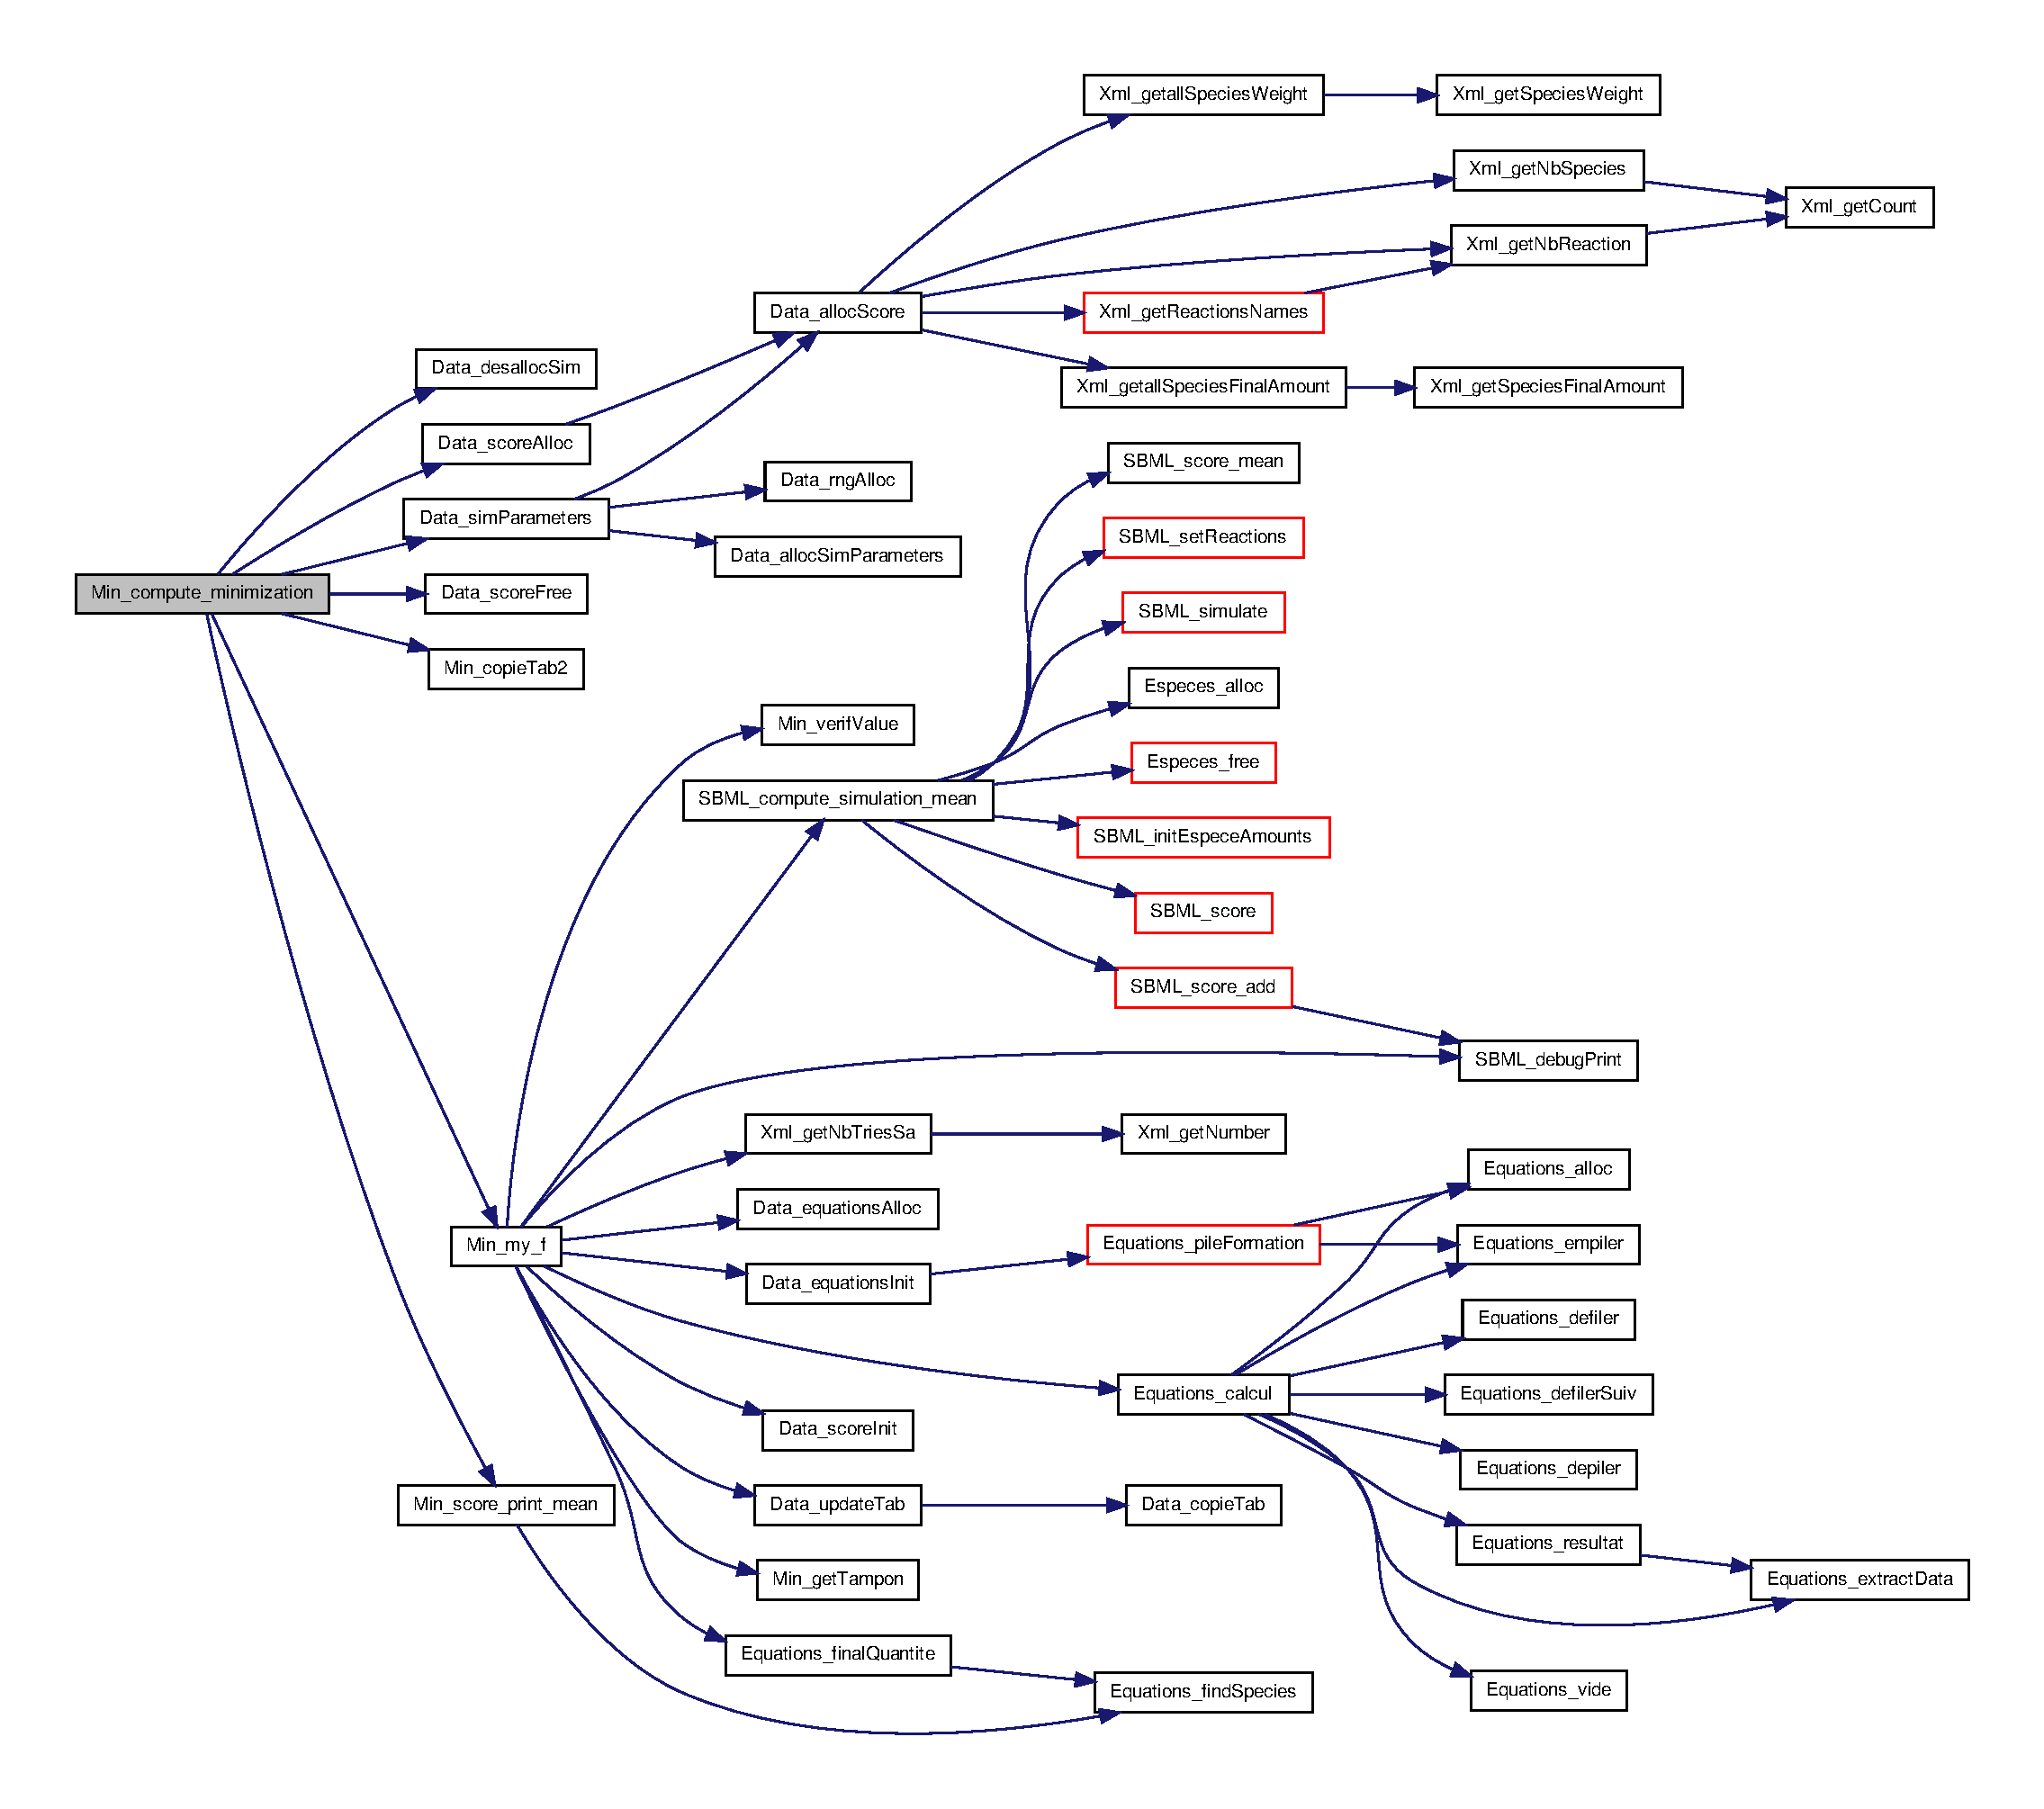
\includegraphics[width=400pt]{gsl__min_8h_a016be27ae853d4d14d48d81c626b1e50_cgraph}
\end{center}
\end{figure}


\hypertarget{gsl__min_8h_a8d981de0373a06da9601e1b5eef379e1}{
\index{gsl\_\-min.h@{gsl\_\-min.h}!Min\_\-copieTab2@{Min\_\-copieTab2}}
\index{Min\_\-copieTab2@{Min\_\-copieTab2}!gsl_min.h@{gsl\_\-min.h}}
\subsubsection[{Min\_\-copieTab2}]{\setlength{\rightskip}{0pt plus 5cm}int Min\_\-copieTab2 (
\begin{DoxyParamCaption}
\item[{double $\ast$}]{x, }
\item[{int}]{current, }
\item[{int}]{debut, }
\item[{int}]{fin}
\end{DoxyParamCaption}
)}}
\label{gsl__min_8h_a8d981de0373a06da9601e1b5eef379e1}


Copy table of reaction parameters. 

\begin{DoxyAuthor}{Author}
Amine Ghozlane 
\end{DoxyAuthor}

\begin{DoxyParams}{Parameters}
{\em x} & Short table of reaction parameters \\
\hline
{\em current} & Line \\
\hline
{\em debut} & Beginning \\
\hline
{\em fin} & End \\
\hline
\end{DoxyParams}
\begin{DoxyReturn}{Returns}
Number of copied element 
\end{DoxyReturn}


Definition at line 68 of file gsl\_\-min.c.



References SimParameters::y.



Referenced by Min\_\-compute\_\-minimization().

\hypertarget{gsl__min_8h_a1f1d9c640473d18e2c9c092428d7052f}{
\index{gsl\_\-min.h@{gsl\_\-min.h}!Min\_\-copieTab3@{Min\_\-copieTab3}}
\index{Min\_\-copieTab3@{Min\_\-copieTab3}!gsl_min.h@{gsl\_\-min.h}}
\subsubsection[{Min\_\-copieTab3}]{\setlength{\rightskip}{0pt plus 5cm}int Min\_\-copieTab3 (
\begin{DoxyParamCaption}
\item[{gsl\_\-multimin\_\-fminimizer $\ast$}]{s, }
\item[{int}]{current, }
\item[{int}]{debut, }
\item[{int}]{fin}
\end{DoxyParamCaption}
)}}
\label{gsl__min_8h_a1f1d9c640473d18e2c9c092428d7052f}


Copy short table of parameter into the larger table. 

\begin{DoxyAuthor}{Author}
Amine Ghozlane 
\end{DoxyAuthor}

\begin{DoxyParams}{Parameters}
{\em s} & Minimizer parameter \\
\hline
{\em current} & Line \\
\hline
{\em debut} & Beginning \\
\hline
{\em fin} & End \\
\hline
\end{DoxyParams}
\begin{DoxyReturn}{Returns}
Number of copied element 
\end{DoxyReturn}


Definition at line 90 of file gsl\_\-min.c.



References SimParameters::y.

\hypertarget{gsl__min_8h_a843d6e8ed1d3354a55586c7734f60499}{
\index{gsl\_\-min.h@{gsl\_\-min.h}!Min\_\-getTampon@{Min\_\-getTampon}}
\index{Min\_\-getTampon@{Min\_\-getTampon}!gsl_min.h@{gsl\_\-min.h}}
\subsubsection[{Min\_\-getTampon}]{\setlength{\rightskip}{0pt plus 5cm}void Min\_\-getTampon (
\begin{DoxyParamCaption}
\item[{double $\ast$}]{energie\_\-temp, }
\item[{double}]{energie}
\end{DoxyParamCaption}
)}}
\label{gsl__min_8h_a843d6e8ed1d3354a55586c7734f60499}


Enter in the program for standard deviation. 

\begin{DoxyAuthor}{Author}
Amine Ghozlane 
\end{DoxyAuthor}

\begin{DoxyParams}{Parameters}
{\em energie\_\-temp} & Current energy \\
\hline
{\em energie} & Best energy \\
\hline
\end{DoxyParams}


Definition at line 208 of file gsl\_\-min.c.



References ListParameters::nb\_\-parameters, SimParameters::out, Score::quantite, Score::taille, and SimParameters::y.



Referenced by Min\_\-my\_\-f().

\hypertarget{gsl__min_8h_ac0cf1b97696b91752884777f11368223}{
\index{gsl\_\-min.h@{gsl\_\-min.h}!Min\_\-my\_\-f@{Min\_\-my\_\-f}}
\index{Min\_\-my\_\-f@{Min\_\-my\_\-f}!gsl_min.h@{gsl\_\-min.h}}
\subsubsection[{Min\_\-my\_\-f}]{\setlength{\rightskip}{0pt plus 5cm}double Min\_\-my\_\-f (
\begin{DoxyParamCaption}
\item[{const gsl\_\-vector $\ast$}]{v, }
\item[{void $\ast$}]{params}
\end{DoxyParamCaption}
)}}
\label{gsl__min_8h_ac0cf1b97696b91752884777f11368223}


Enter in the program for standard deviation. 

\begin{DoxyAuthor}{Author}
Amine Ghozlane 
\end{DoxyAuthor}

\begin{DoxyParams}{Parameters}
{\em v} & Vector of reaction parameters \\
\hline
{\em params} & Unused parameter define by GSL \\
\hline
\end{DoxyParams}
\begin{DoxyReturn}{Returns}
Energy value 
\end{DoxyReturn}


Definition at line 149 of file gsl\_\-min.c.



References ListParameters::banned, ListParameters::conf, Data\_\-equationsAlloc(), Data\_\-equationsInit(), Data\_\-scoreInit(), Data\_\-updateTab(), SimParameters::debugFile, Equations\_\-calcul(), Equations\_\-finalQuantite(), Min\_\-getTampon(), Min\_\-verifValue(), ListParameters::model, Score::name, ListParameters::nb\_\-banned, ListParameters::nb\_\-couples, ListParameters::nb\_\-equations, ListParameters::nb\_\-parameters, Score::nb\_\-species, SimParameters::out, ListParameters::parameters, SimParameters::pile, Score::quantite, SimParameters::r, SBML\_\-compute\_\-simulation\_\-mean(), SBML\_\-debugPrint(), Score::species, Score::species\_\-amount, Score::species\_\-weight, Score::taille, Score::tailleSpecies, Xml\_\-getNbTriesSa(), and SimParameters::y.



Referenced by Min\_\-compute\_\-minimization().



Here is the call graph for this function:\nopagebreak
\begin{figure}[H]
\begin{center}
\leavevmode
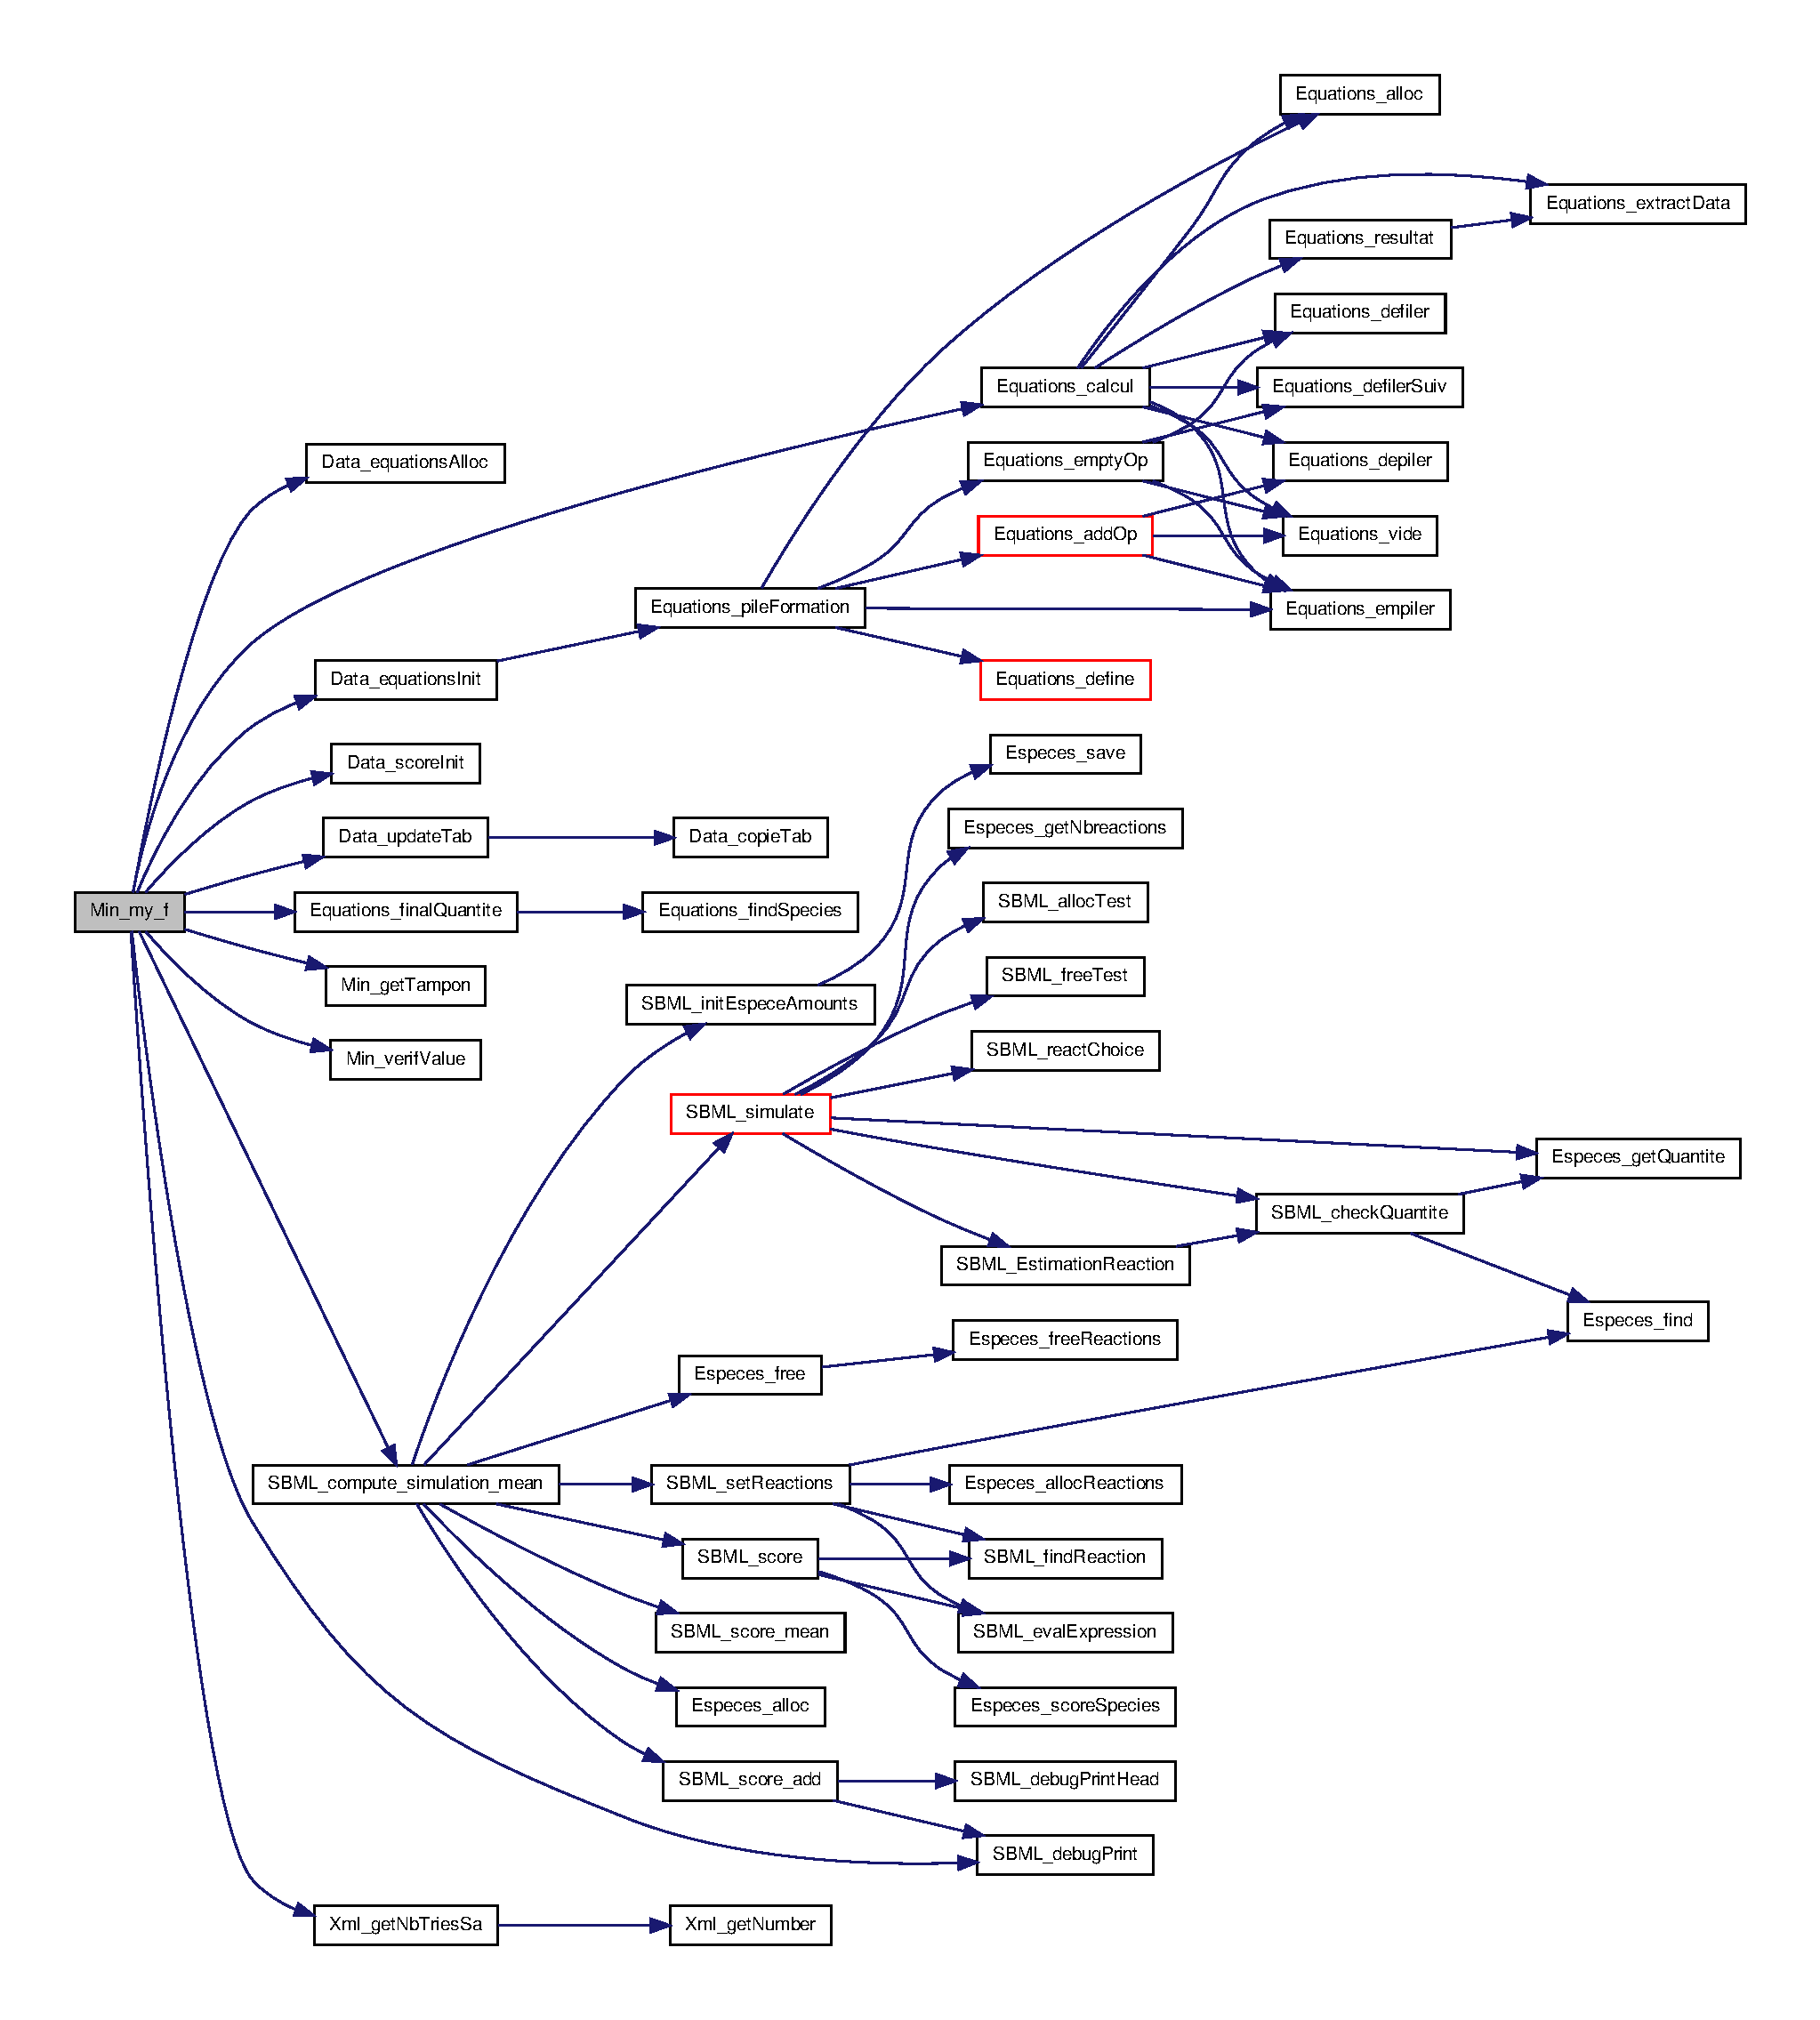
\includegraphics[width=400pt]{gsl__min_8h_ac0cf1b97696b91752884777f11368223_cgraph}
\end{center}
\end{figure}


\hypertarget{gsl__min_8h_a6fc9a31eec661815e3b5b83fc196d652}{
\index{gsl\_\-min.h@{gsl\_\-min.h}!Min\_\-score\_\-print\_\-mean@{Min\_\-score\_\-print\_\-mean}}
\index{Min\_\-score\_\-print\_\-mean@{Min\_\-score\_\-print\_\-mean}!gsl_min.h@{gsl\_\-min.h}}
\subsubsection[{Min\_\-score\_\-print\_\-mean}]{\setlength{\rightskip}{0pt plus 5cm}void Min\_\-score\_\-print\_\-mean (
\begin{DoxyParamCaption}
\item[{double $\ast$}]{result\_\-tab}
\end{DoxyParamCaption}
)}}
\label{gsl__min_8h_a6fc9a31eec661815e3b5b83fc196d652}


Save the minimization result. 

\begin{DoxyAuthor}{Author}
Amine Ghozlane 
\end{DoxyAuthor}

\begin{DoxyParams}{Parameters}
{\em result\_\-tab} & Result table \\
\hline
\end{DoxyParams}


Definition at line 230 of file gsl\_\-min.c.



References Equations\_\-findSpecies(), Score::name, ListParameters::nb\_\-parameters, Score::nb\_\-species, SimParameters::out, Score::quantite, Score::species, Score::species\_\-amount, Score::taille, Score::tailleSpecies, and SimParameters::y.



Referenced by Min\_\-compute\_\-minimization().



Here is the call graph for this function:\nopagebreak
\begin{figure}[H]
\begin{center}
\leavevmode
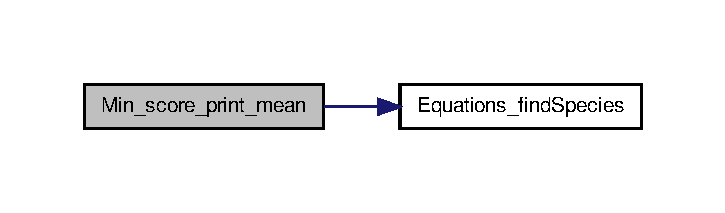
\includegraphics[width=348pt]{gsl__min_8h_a6fc9a31eec661815e3b5b83fc196d652_cgraph}
\end{center}
\end{figure}


\hypertarget{gsl__min_8h_a2d2f0b8fd130c026d88c29339e3766fa}{
\index{gsl\_\-min.h@{gsl\_\-min.h}!Min\_\-verifValue@{Min\_\-verifValue}}
\index{Min\_\-verifValue@{Min\_\-verifValue}!gsl_min.h@{gsl\_\-min.h}}
\subsubsection[{Min\_\-verifValue}]{\setlength{\rightskip}{0pt plus 5cm}void Min\_\-verifValue (
\begin{DoxyParamCaption}
\item[{gsl\_\-vector $\ast$}]{v, }
\item[{double $\ast$}]{x, }
\item[{int}]{debut, }
\item[{int}]{max}
\end{DoxyParamCaption}
)}}
\label{gsl__min_8h_a2d2f0b8fd130c026d88c29339e3766fa}


Checking reaction ratio parameters. 

\begin{DoxyAuthor}{Author}
Amine Ghozlane 
\end{DoxyAuthor}

\begin{DoxyParams}{Parameters}
{\em v} & Vector of reaction parameters \\
\hline
{\em x} & Short table of reaction parameters \\
\hline
{\em debut} & Beginning \\
\hline
{\em max} & End \\
\hline
\end{DoxyParams}


Definition at line 114 of file gsl\_\-min.c.



Referenced by Min\_\-my\_\-f().


\hypertarget{gsl__mod_8h}{
\section{metaboflux/include/gsl\_\-mod.h File Reference}
\label{gsl__mod_8h}\index{metaboflux/include/gsl\_\-mod.h@{metaboflux/include/gsl\_\-mod.h}}
}


Compute the modeling of scenarii.  


This graph shows which files directly or indirectly include this file:\nopagebreak
\begin{figure}[H]
\begin{center}
\leavevmode
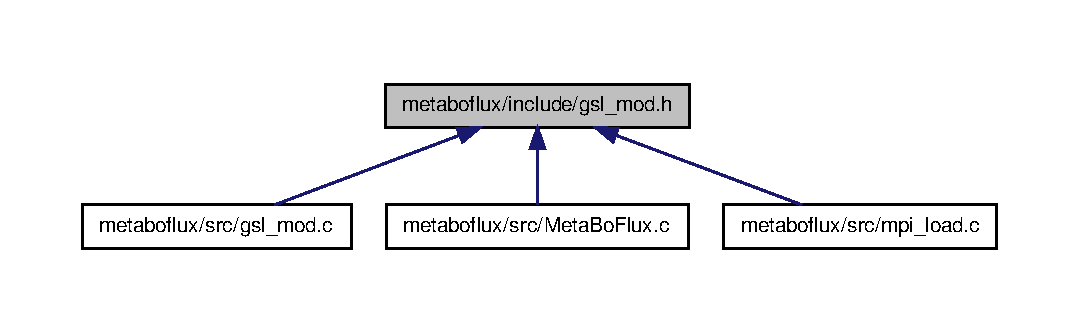
\includegraphics[width=400pt]{gsl__mod_8h__dep__incl}
\end{center}
\end{figure}
\subsection*{Functions}
\begin{DoxyCompactItemize}
\item 
void \hyperlink{gsl__mod_8h_a97dc18e0e086fa391d82d703cc470bc8}{Mod\_\-score\_\-print\_\-mean} (\hyperlink{structListParameters}{pListParameters}, \hyperlink{structSimParameters}{pSimParameters}, double $\ast$, double, int, int)
\begin{DoxyCompactList}\small\item\em Print the mean score. \end{DoxyCompactList}\item 
void \hyperlink{gsl__mod_8h_af23349f6e6b94ecae16caf9b7837eb06}{Mod\_\-compute\_\-modeling} (\hyperlink{structListParameters}{pListParameters}, double $\ast$, double $\ast$, char $\ast$$\ast$, int, int, int)
\begin{DoxyCompactList}\small\item\em Compute the modeling. \end{DoxyCompactList}\end{DoxyCompactItemize}


\subsection{Detailed Description}
Compute the modeling of scenarii. This file is part of MetaBoFlux (\href{http://www.cbib.u-bordeaux2.fr/metaboflux/}{\tt http://www.cbib.u-\/bordeaux2.fr/metaboflux/}) Copyright (C) 2010 Amine Ghozlane from LaBRI and University of Bordeaux 1

MetaBoFlux is free software: you can redistribute it and/or modify it under the terms of the GNU Lesser General Public License as published by the Free Software Foundation, either version 3 of the License, or (at your option) any later version.

MetaBoFlux is distributed in the hope that it will be useful, but WITHOUT ANY WARRANTY; without even the implied warranty of MERCHANTABILITY or FITNESS FOR A PARTICULAR PURPOSE. See the GNU General Public License for more details.

You should have received a copy of the GNU Lesser General Public License along with this program. If not, see $<$\href{http://www.gnu.org/licenses/}{\tt http://www.gnu.org/licenses/}$>$.

\begin{DoxyAuthor}{Author}
\{Amine Ghozlane\} 
\end{DoxyAuthor}
\begin{DoxyVersion}{Version}
2.0 
\end{DoxyVersion}
\begin{DoxyDate}{Date}
9 novembre 2009 
\end{DoxyDate}


Definition in file \hyperlink{gsl__mod_8h_source}{gsl\_\-mod.h}.



\subsection{Function Documentation}
\hypertarget{gsl__mod_8h_af23349f6e6b94ecae16caf9b7837eb06}{
\index{gsl\_\-mod.h@{gsl\_\-mod.h}!Mod\_\-compute\_\-modeling@{Mod\_\-compute\_\-modeling}}
\index{Mod\_\-compute\_\-modeling@{Mod\_\-compute\_\-modeling}!gsl_mod.h@{gsl\_\-mod.h}}
\subsubsection[{Mod\_\-compute\_\-modeling}]{\setlength{\rightskip}{0pt plus 5cm}void Mod\_\-compute\_\-modeling (
\begin{DoxyParamCaption}
\item[{{\bf pListParameters}}]{a, }
\item[{double $\ast$}]{fluxRatio, }
\item[{double $\ast$}]{result\_\-tab, }
\item[{char $\ast$$\ast$}]{files\_\-path, }
\item[{int}]{number\_\-group, }
\item[{int}]{group, }
\item[{int}]{debug}
\end{DoxyParamCaption}
)}}
\label{gsl__mod_8h_af23349f6e6b94ecae16caf9b7837eb06}


Compute the modeling. 

\begin{DoxyAuthor}{Author}
Amine Ghozlane 
\end{DoxyAuthor}

\begin{DoxyParams}{Parameters}
{\em a} & struct \hyperlink{structListParameters}{ListParameters} \\
\hline
{\em fluxRatio} & Ratio parameters \\
\hline
{\em result\_\-tab} & Result table \\
\hline
{\em files\_\-path} & List of paths \\
\hline
{\em number\_\-group} & Number of the group \\
\hline
{\em group} & Group flag \\
\hline
{\em debug} & Debug flag \\
\hline
\end{DoxyParams}


Definition at line 109 of file gsl\_\-mod.c.



References ListParameters::banned, ListParameters::conf, Data\_\-desallocSim(), Data\_\-equationsAlloc(), Data\_\-equationsInit(), Data\_\-scoreAlloc(), Data\_\-scoreFree(), Data\_\-simParameters(), SimParameters::debugFile, Equations\_\-calcul(), Equations\_\-finalQuantite(), Mod\_\-score\_\-print\_\-mean(), ListParameters::model, Score::name, ListParameters::nb\_\-banned, ListParameters::nb\_\-equations, ListParameters::nb\_\-parameters, Score::nb\_\-species, SimParameters::out, SimParameters::pile, Score::quantite, SimParameters::r, SBML\_\-compute\_\-simulation\_\-mean(), SBML\_\-debugPrint(), Score::species, Score::species\_\-amount, Score::species\_\-weight, Score::taille, Score::tailleSpecies, Xml\_\-getNbTriesMod(), and SimParameters::y.



Referenced by Mpi\_\-slave().



Here is the call graph for this function:\nopagebreak
\begin{figure}[H]
\begin{center}
\leavevmode
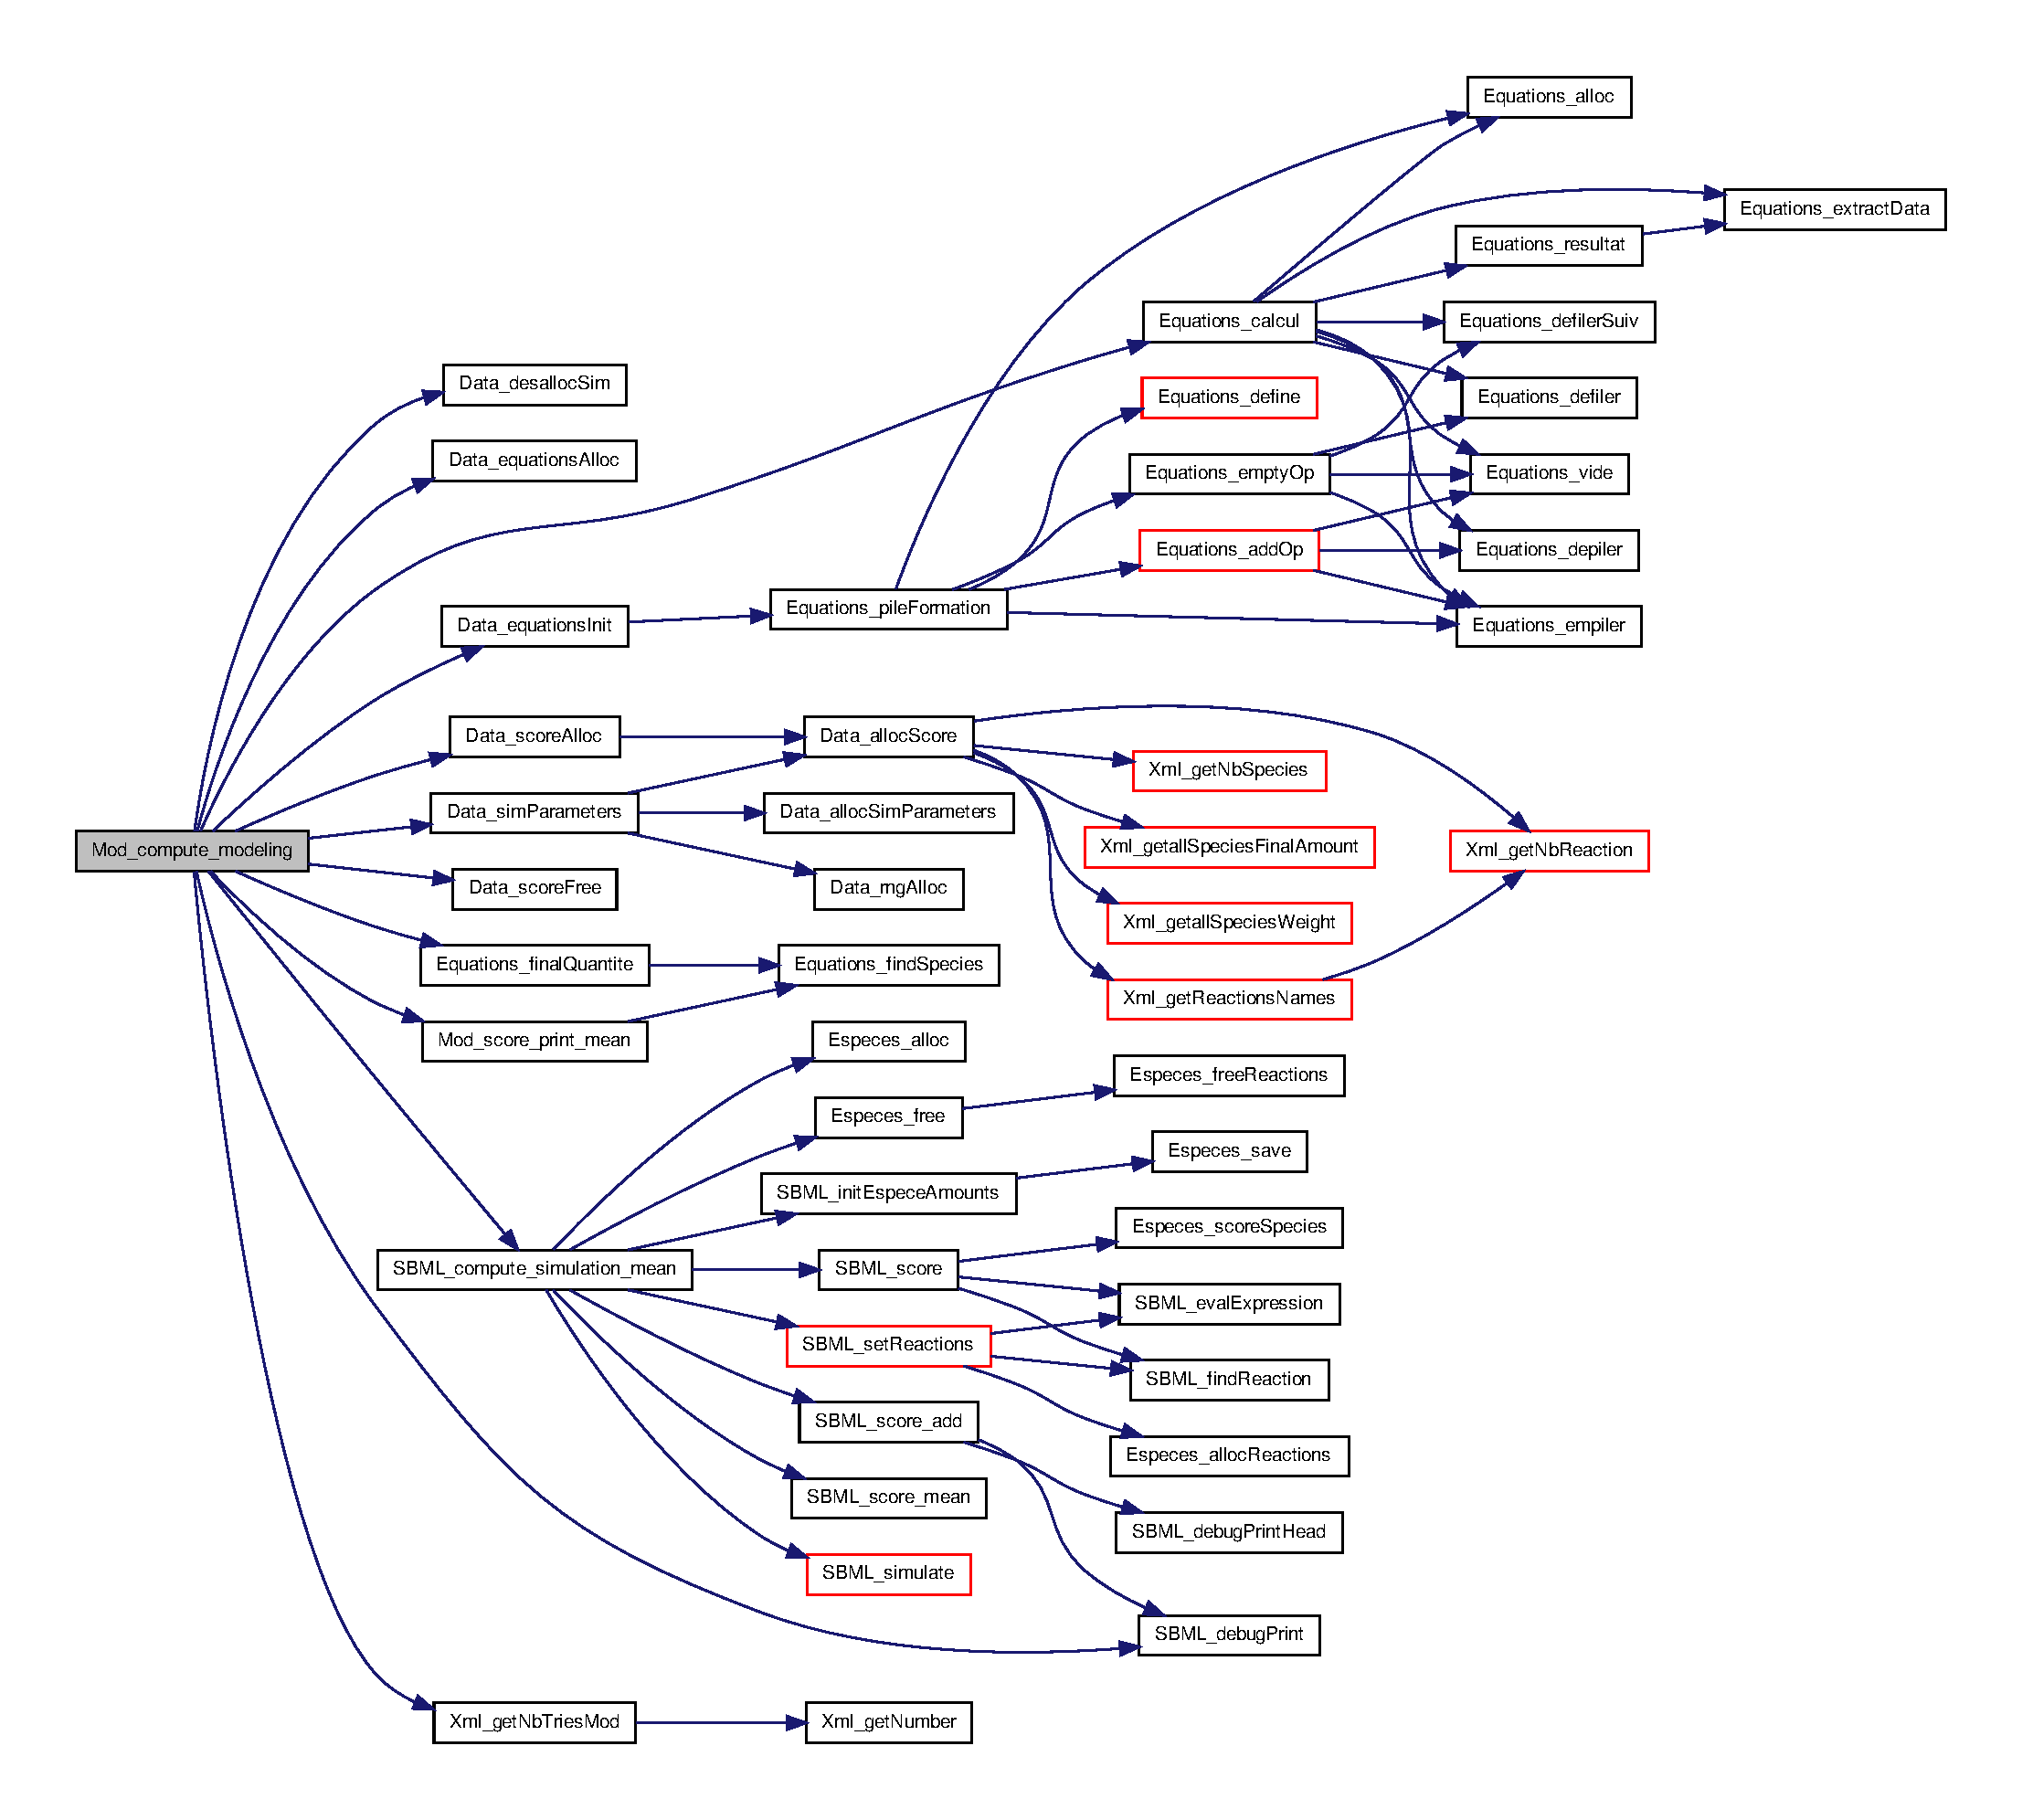
\includegraphics[width=400pt]{gsl__mod_8h_af23349f6e6b94ecae16caf9b7837eb06_cgraph}
\end{center}
\end{figure}


\hypertarget{gsl__mod_8h_a97dc18e0e086fa391d82d703cc470bc8}{
\index{gsl\_\-mod.h@{gsl\_\-mod.h}!Mod\_\-score\_\-print\_\-mean@{Mod\_\-score\_\-print\_\-mean}}
\index{Mod\_\-score\_\-print\_\-mean@{Mod\_\-score\_\-print\_\-mean}!gsl_mod.h@{gsl\_\-mod.h}}
\subsubsection[{Mod\_\-score\_\-print\_\-mean}]{\setlength{\rightskip}{0pt plus 5cm}void Mod\_\-score\_\-print\_\-mean (
\begin{DoxyParamCaption}
\item[{{\bf pListParameters}}]{a, }
\item[{{\bf pSimParameters}}]{simu, }
\item[{double $\ast$}]{result\_\-tab, }
\item[{double}]{energie, }
\item[{int}]{number\_\-group, }
\item[{int}]{group}
\end{DoxyParamCaption}
)}}
\label{gsl__mod_8h_a97dc18e0e086fa391d82d703cc470bc8}


Print the mean score. 

\begin{DoxyAuthor}{Author}
Amine Ghozlane 
\end{DoxyAuthor}

\begin{DoxyParams}{Parameters}
{\em a} & Global parameters \\
\hline
{\em simu} & Simulation parameters \\
\hline
{\em result\_\-tab} & Result table \\
\hline
{\em energie} & Energy of the simulation \\
\hline
{\em number\_\-group} & Number of simulation \\
\hline
{\em group} & Number of the group (if a group is simulated) \\
\hline
\end{DoxyParams}


Definition at line 58 of file gsl\_\-mod.c.



References Equations\_\-findSpecies(), Score::name, ListParameters::nb\_\-parameters, Score::nb\_\-species, SimParameters::out, Score::quantite, Score::species, Score::species\_\-amount, Score::taille, Score::tailleSpecies, and SimParameters::y.



Referenced by Mod\_\-compute\_\-modeling().



Here is the call graph for this function:\nopagebreak
\begin{figure}[H]
\begin{center}
\leavevmode
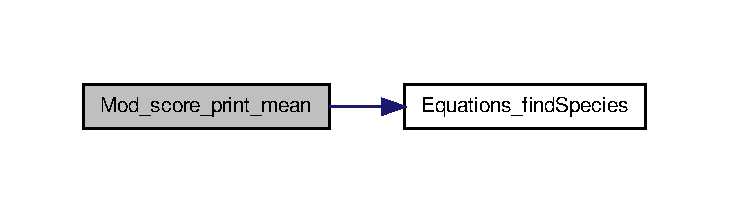
\includegraphics[width=350pt]{gsl__mod_8h_a97dc18e0e086fa391d82d703cc470bc8_cgraph}
\end{center}
\end{figure}



\hypertarget{gsl__recuit_8h}{
\section{metaboflux/include/gsl\_\-recuit.h File Reference}
\label{gsl__recuit_8h}\index{metaboflux/include/gsl\_\-recuit.h@{metaboflux/include/gsl\_\-recuit.h}}
}


Compute the simulated annealing.  


This graph shows which files directly or indirectly include this file:\nopagebreak
\begin{figure}[H]
\begin{center}
\leavevmode
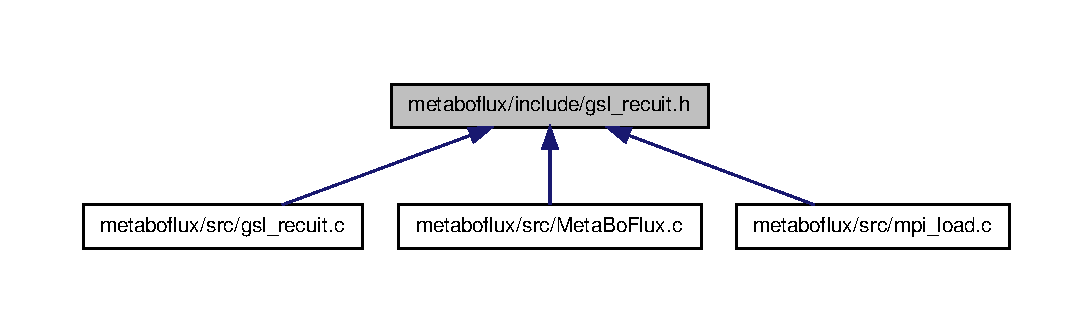
\includegraphics[width=400pt]{gsl__recuit_8h__dep__incl}
\end{center}
\end{figure}
\subsection*{Functions}
\begin{DoxyCompactItemize}
\item 
double \hyperlink{gsl__recuit_8h_a76e1fe1e0d6471f07f55bcf28d247fa5}{Recuit\_\-energyFunction} (void $\ast$)
\begin{DoxyCompactList}\small\item\em Simulate the petri net and compute the energy. \end{DoxyCompactList}\item 
double \hyperlink{gsl__recuit_8h_a262f0cba7cb59023d3b45bc17c103aac}{Recuit\_\-metricDistance} (void $\ast$, void $\ast$)
\begin{DoxyCompactList}\small\item\em Compute the distance between the two table. \end{DoxyCompactList}\item 
void \hyperlink{gsl__recuit_8h_a992371555f490f726cbe4a1c90785a09}{Recuit\_\-takeStep} (const gsl\_\-rng $\ast$, void $\ast$, double)
\begin{DoxyCompactList}\small\item\em Take a step through the solution space TSP. \end{DoxyCompactList}\item 
void \hyperlink{gsl__recuit_8h_afd9db376bfecbe387f3836854c31f6d0}{Recuit\_\-printPosition} (void $\ast$)
\begin{DoxyCompactList}\small\item\em Print the table of reaction parameters. \end{DoxyCompactList}\item 
FILE $\ast$ \hyperlink{gsl__recuit_8h_a50384383f4c2a13a1f7dc85f69339bd6}{Recuit\_\-redirectionFlux} (\hyperlink{structxmlConfig__t}{xmlConfig\_\-t} $\ast$, FILE $\ast$, char $\ast$$\ast$, int)
\begin{DoxyCompactList}\small\item\em Redirect stdout flux. \end{DoxyCompactList}\item 
void \hyperlink{gsl__recuit_8h_acc458cd24422d89b326a1b4bb7940cbf}{Recuit\_\-verifParameters} (double $\ast$, const gsl\_\-rng $\ast$, int, int)
\begin{DoxyCompactList}\small\item\em Choice of parameters and verification of their value. \end{DoxyCompactList}\item 
void \hyperlink{gsl__recuit_8h_a389f2f70421b758b2eaea08d8ef9033a}{Recuit\_\-verifParameters\_\-2} (double $\ast$, double $\ast$, const gsl\_\-rng $\ast$, int, int, double)
\begin{DoxyCompactList}\small\item\em Choice of parameters and verification of their value. \end{DoxyCompactList}\item 
void \hyperlink{gsl__recuit_8h_aa83d3ab8e9c0f5d45ddedf1b65a67f98}{Recuit\_\-defParametre} (double $\ast$, const gsl\_\-rng $\ast$)
\begin{DoxyCompactList}\small\item\em Definition of the initial parameters of the simulation. \end{DoxyCompactList}\item 
void \hyperlink{gsl__recuit_8h_a41e47a5713188f196ebc7a66a9052d3d}{Recuit\_\-printParametre} (double $\ast$)
\begin{DoxyCompactList}\small\item\em Print initial parameters. \end{DoxyCompactList}\item 
void \hyperlink{gsl__recuit_8h_adde03ef6388e6b9b06eefbfa685c2ee0}{Recuit\_\-compute\_\-recuit} (char $\ast$$\ast$, int, int, \hyperlink{structListParameters}{pListParameters}, gsl\_\-siman\_\-params\_\-t)
\begin{DoxyCompactList}\small\item\em Compute the simulated annealing. \end{DoxyCompactList}\end{DoxyCompactItemize}


\subsection{Detailed Description}
Compute the simulated annealing. This file is part of MetaBoFlux (\href{http://www.cbib.u-bordeaux2.fr/metaboflux/}{\tt http://www.cbib.u-\/bordeaux2.fr/metaboflux/}) Copyright (C) 2010 Amine Ghozlane from LaBRI and University of Bordeaux 1

MetaBoFlux is free software: you can redistribute it and/or modify it under the terms of the GNU Lesser General Public License as published by the Free Software Foundation, either version 3 of the License, or (at your option) any later version.

MetaBoFlux is distributed in the hope that it will be useful, but WITHOUT ANY WARRANTY; without even the implied warranty of MERCHANTABILITY or FITNESS FOR A PARTICULAR PURPOSE. See the GNU General Public License for more details.

You should have received a copy of the GNU Lesser General Public License along with this program. If not, see $<$\href{http://www.gnu.org/licenses/}{\tt http://www.gnu.org/licenses/}$>$.

\begin{DoxyAuthor}{Author}
\{Amine Ghozlane\} 
\end{DoxyAuthor}
\begin{DoxyVersion}{Version}
2.0 
\end{DoxyVersion}
\begin{DoxyDate}{Date}
9 novembre 2009 
\end{DoxyDate}


Definition in file \hyperlink{gsl__recuit_8h_source}{gsl\_\-recuit.h}.



\subsection{Function Documentation}
\hypertarget{gsl__recuit_8h_adde03ef6388e6b9b06eefbfa685c2ee0}{
\index{gsl\_\-recuit.h@{gsl\_\-recuit.h}!Recuit\_\-compute\_\-recuit@{Recuit\_\-compute\_\-recuit}}
\index{Recuit\_\-compute\_\-recuit@{Recuit\_\-compute\_\-recuit}!gsl_recuit.h@{gsl\_\-recuit.h}}
\subsubsection[{Recuit\_\-compute\_\-recuit}]{\setlength{\rightskip}{0pt plus 5cm}void Recuit\_\-compute\_\-recuit (
\begin{DoxyParamCaption}
\item[{char $\ast$$\ast$}]{files\_\-path, }
\item[{int}]{debug, }
\item[{int}]{number, }
\item[{{\bf pListParameters}}]{allone, }
\item[{gsl\_\-siman\_\-params\_\-t}]{params}
\end{DoxyParamCaption}
)}}
\label{gsl__recuit_8h_adde03ef6388e6b9b06eefbfa685c2ee0}


Compute the simulated annealing. 

\begin{DoxyAuthor}{Author}
Amine Ghozlane 
\end{DoxyAuthor}

\begin{DoxyParams}{Parameters}
{\em files\_\-path} & List of paths \\
\hline
{\em debug} & Debug flag \\
\hline
{\em number} & Number of the simulation \\
\hline
{\em allone} & Global parameters : struct \hyperlink{structListParameters}{ListParameters} \\
\hline
{\em params} & Gsl parameters \\
\hline
\end{DoxyParams}


Definition at line 304 of file gsl\_\-recuit.c.



References ListParameters::conf, Data\_\-desallocSim(), Data\_\-scoreAlloc(), Data\_\-scoreFree(), Data\_\-simParameters(), ListParameters::interest\_\-parameters, SimParameters::r, Recuit\_\-defParametre(), Recuit\_\-energyFunction(), Recuit\_\-metricDistance(), Recuit\_\-printParametre(), Recuit\_\-printPosition(), Recuit\_\-redirectionFlux(), and Recuit\_\-takeStep().



Referenced by Mpi\_\-slave().



Here is the call graph for this function:\nopagebreak
\begin{figure}[H]
\begin{center}
\leavevmode
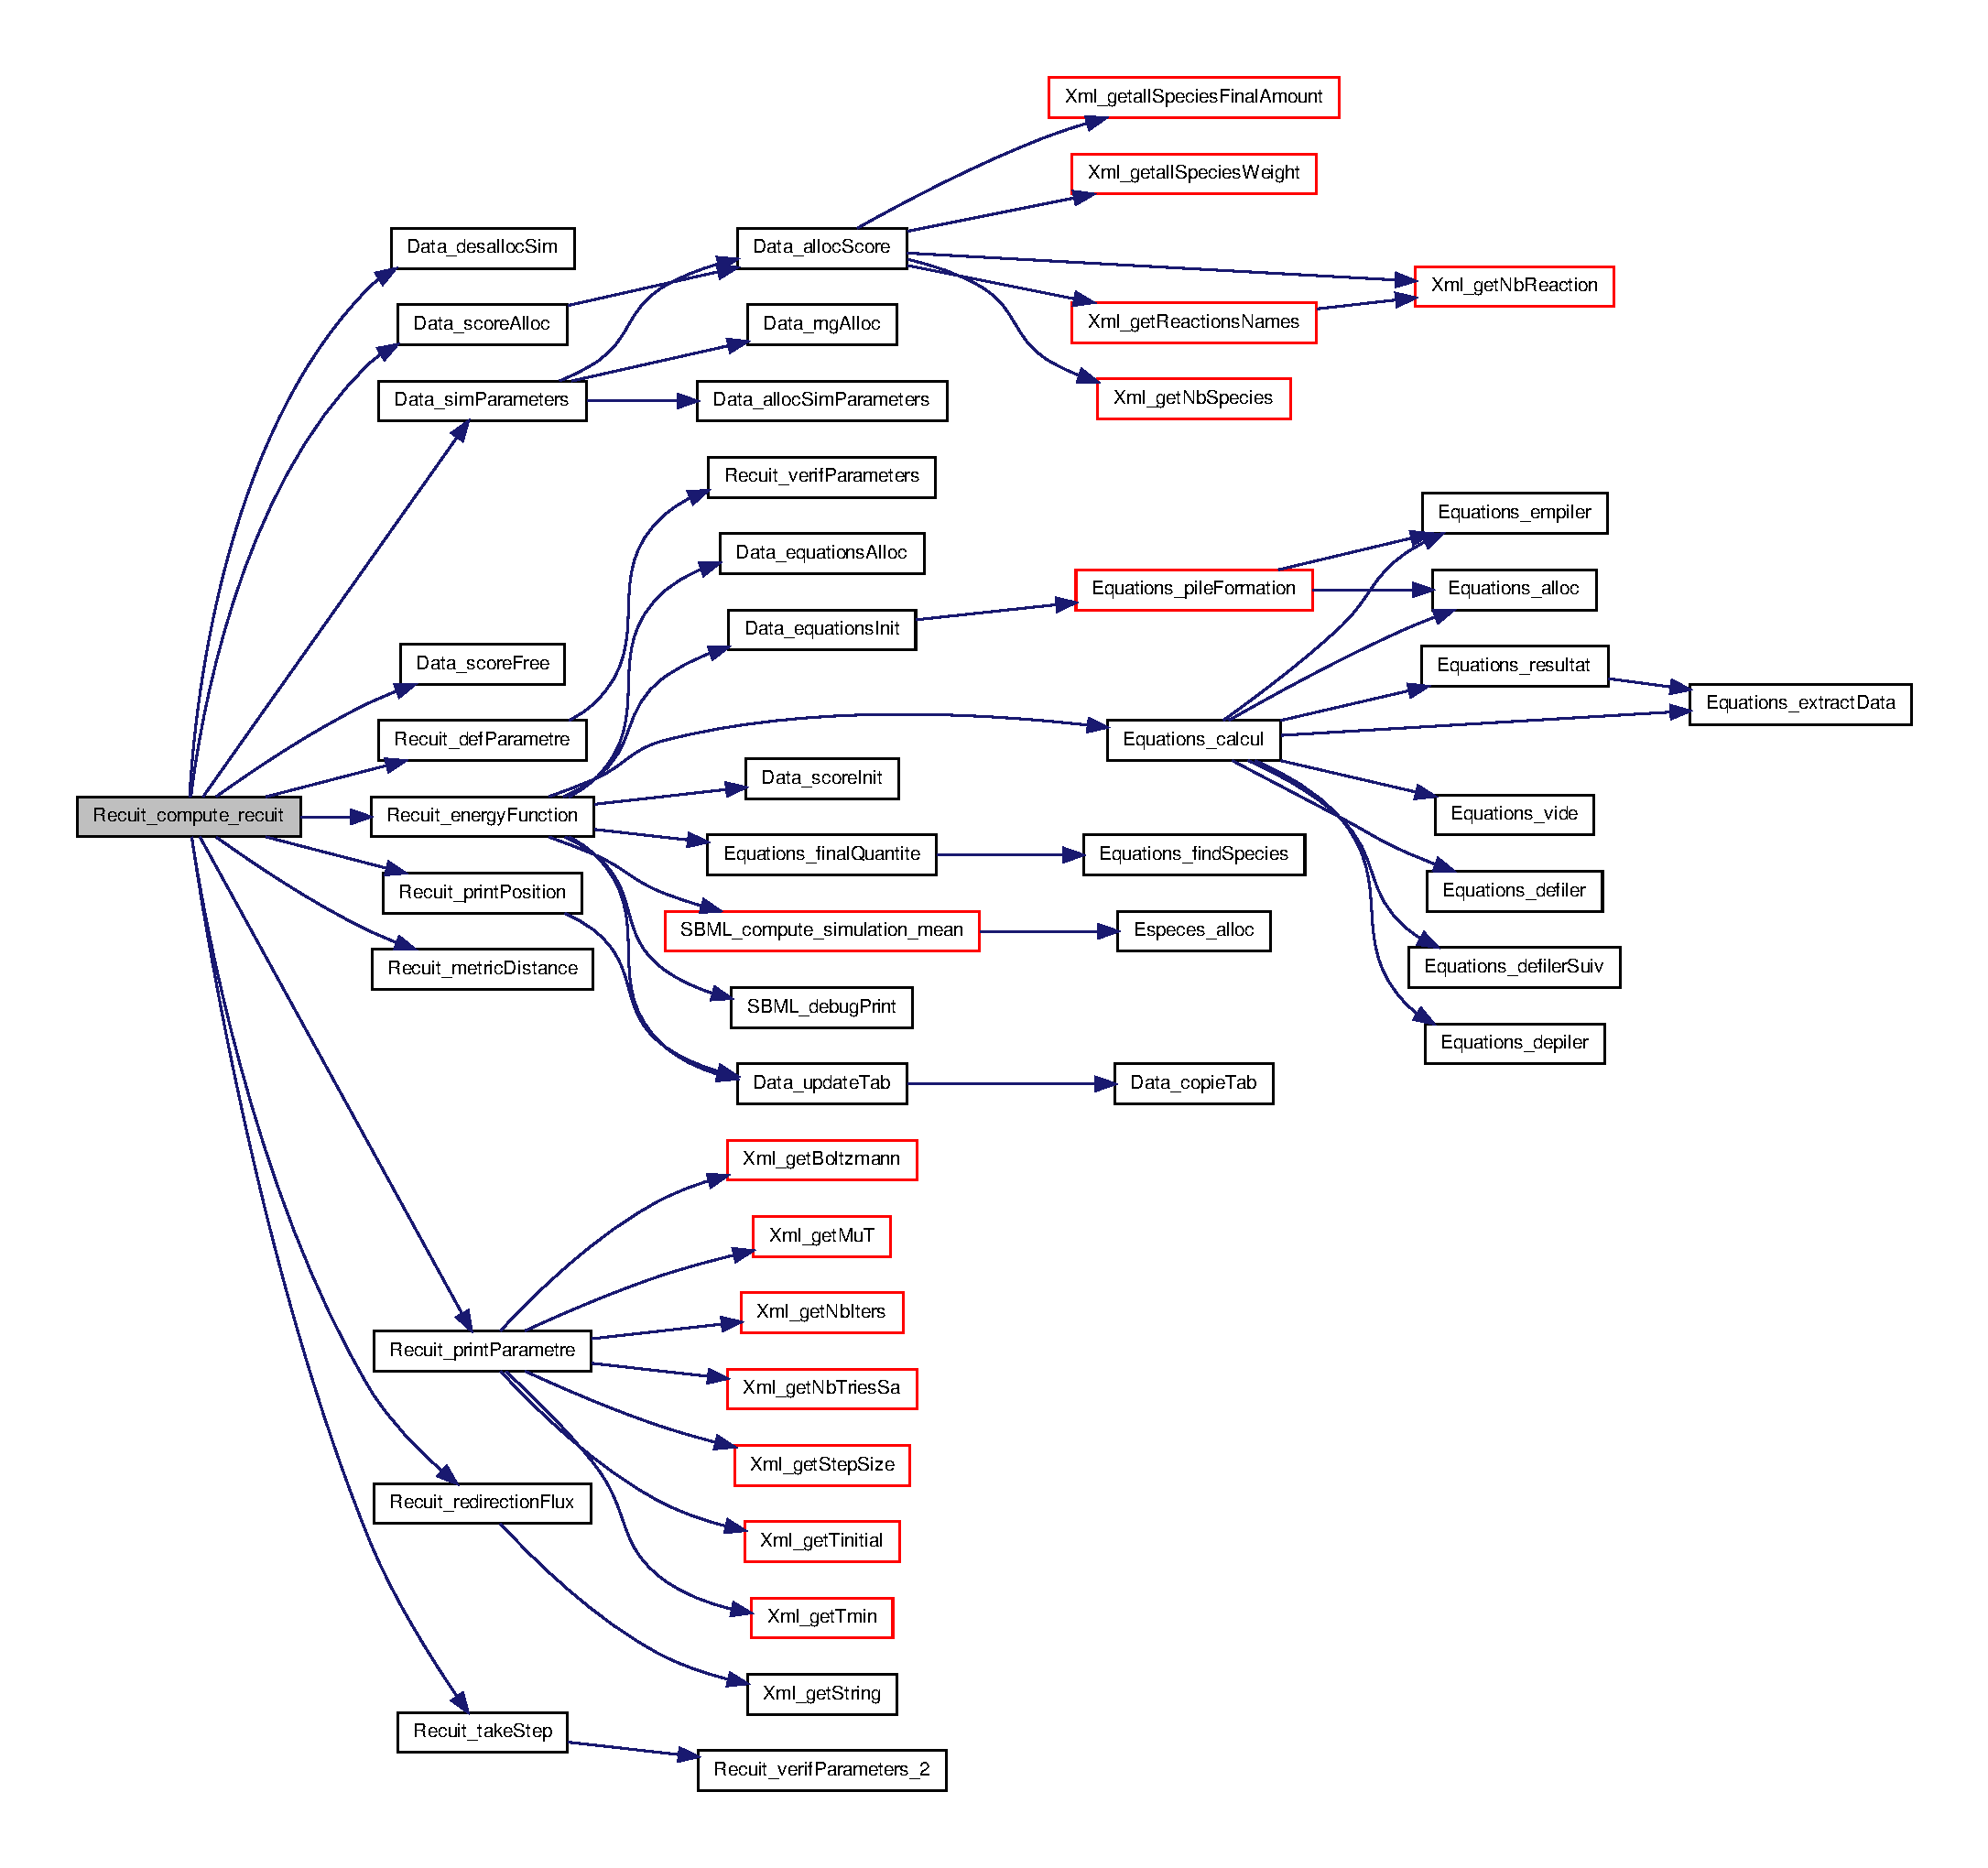
\includegraphics[width=400pt]{gsl__recuit_8h_adde03ef6388e6b9b06eefbfa685c2ee0_cgraph}
\end{center}
\end{figure}


\hypertarget{gsl__recuit_8h_aa83d3ab8e9c0f5d45ddedf1b65a67f98}{
\index{gsl\_\-recuit.h@{gsl\_\-recuit.h}!Recuit\_\-defParametre@{Recuit\_\-defParametre}}
\index{Recuit\_\-defParametre@{Recuit\_\-defParametre}!gsl_recuit.h@{gsl\_\-recuit.h}}
\subsubsection[{Recuit\_\-defParametre}]{\setlength{\rightskip}{0pt plus 5cm}void Recuit\_\-defParametre (
\begin{DoxyParamCaption}
\item[{double $\ast$}]{x\_\-initial, }
\item[{const gsl\_\-rng $\ast$}]{r}
\end{DoxyParamCaption}
)}}
\label{gsl__recuit_8h_aa83d3ab8e9c0f5d45ddedf1b65a67f98}


Definition of the initial parameters of the simulation. 

\begin{DoxyAuthor}{Author}
Amine Ghozlane 
\end{DoxyAuthor}

\begin{DoxyParams}{Parameters}
{\em x\_\-initial} & table of reaction parameters \\
\hline
{\em r} & Random number generator \\
\hline
\end{DoxyParams}


Definition at line 261 of file gsl\_\-recuit.c.



References ListParameters::nb\_\-couples, ListParameters::parameters, and Recuit\_\-verifParameters().



Referenced by Recuit\_\-compute\_\-recuit().



Here is the call graph for this function:\nopagebreak
\begin{figure}[H]
\begin{center}
\leavevmode
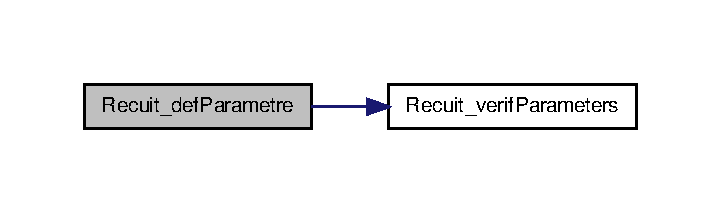
\includegraphics[width=346pt]{gsl__recuit_8h_aa83d3ab8e9c0f5d45ddedf1b65a67f98_cgraph}
\end{center}
\end{figure}


\hypertarget{gsl__recuit_8h_a76e1fe1e0d6471f07f55bcf28d247fa5}{
\index{gsl\_\-recuit.h@{gsl\_\-recuit.h}!Recuit\_\-energyFunction@{Recuit\_\-energyFunction}}
\index{Recuit\_\-energyFunction@{Recuit\_\-energyFunction}!gsl_recuit.h@{gsl\_\-recuit.h}}
\subsubsection[{Recuit\_\-energyFunction}]{\setlength{\rightskip}{0pt plus 5cm}double Recuit\_\-energyFunction (
\begin{DoxyParamCaption}
\item[{void $\ast$}]{xp}
\end{DoxyParamCaption}
)}}
\label{gsl__recuit_8h_a76e1fe1e0d6471f07f55bcf28d247fa5}


Simulate the petri net and compute the energy. 

double \hyperlink{gsl__recuit_8h_a76e1fe1e0d6471f07f55bcf28d247fa5}{Recuit\_\-energyFunction(void $\ast$xp)} \begin{DoxyAuthor}{Author}
Amine Ghozlane 
\end{DoxyAuthor}

\begin{DoxyParams}{Parameters}
{\em xp} & Short table of reaction parameters \\
\hline
\end{DoxyParams}
\begin{DoxyReturn}{Returns}
Energy value 
\end{DoxyReturn}


Definition at line 65 of file gsl\_\-recuit.c.



References ListParameters::banned, Data\_\-equationsAlloc(), Data\_\-equationsInit(), Data\_\-scoreInit(), Data\_\-updateTab(), SimParameters::debugFile, Equations\_\-calcul(), Equations\_\-finalQuantite(), ListParameters::model, Score::name, ListParameters::nb\_\-banned, ListParameters::nb\_\-equations, Score::nb\_\-species, ListParameters::nb\_\-triesSa, SimParameters::out, SimParameters::pile, Score::quantite, SimParameters::r, SBML\_\-compute\_\-simulation\_\-mean(), SBML\_\-debugPrint(), Score::species, Score::species\_\-amount, Score::species\_\-weight, Score::taille, Score::tailleSpecies, and SimParameters::y.



Referenced by Recuit\_\-compute\_\-recuit().



Here is the call graph for this function:\nopagebreak
\begin{figure}[H]
\begin{center}
\leavevmode
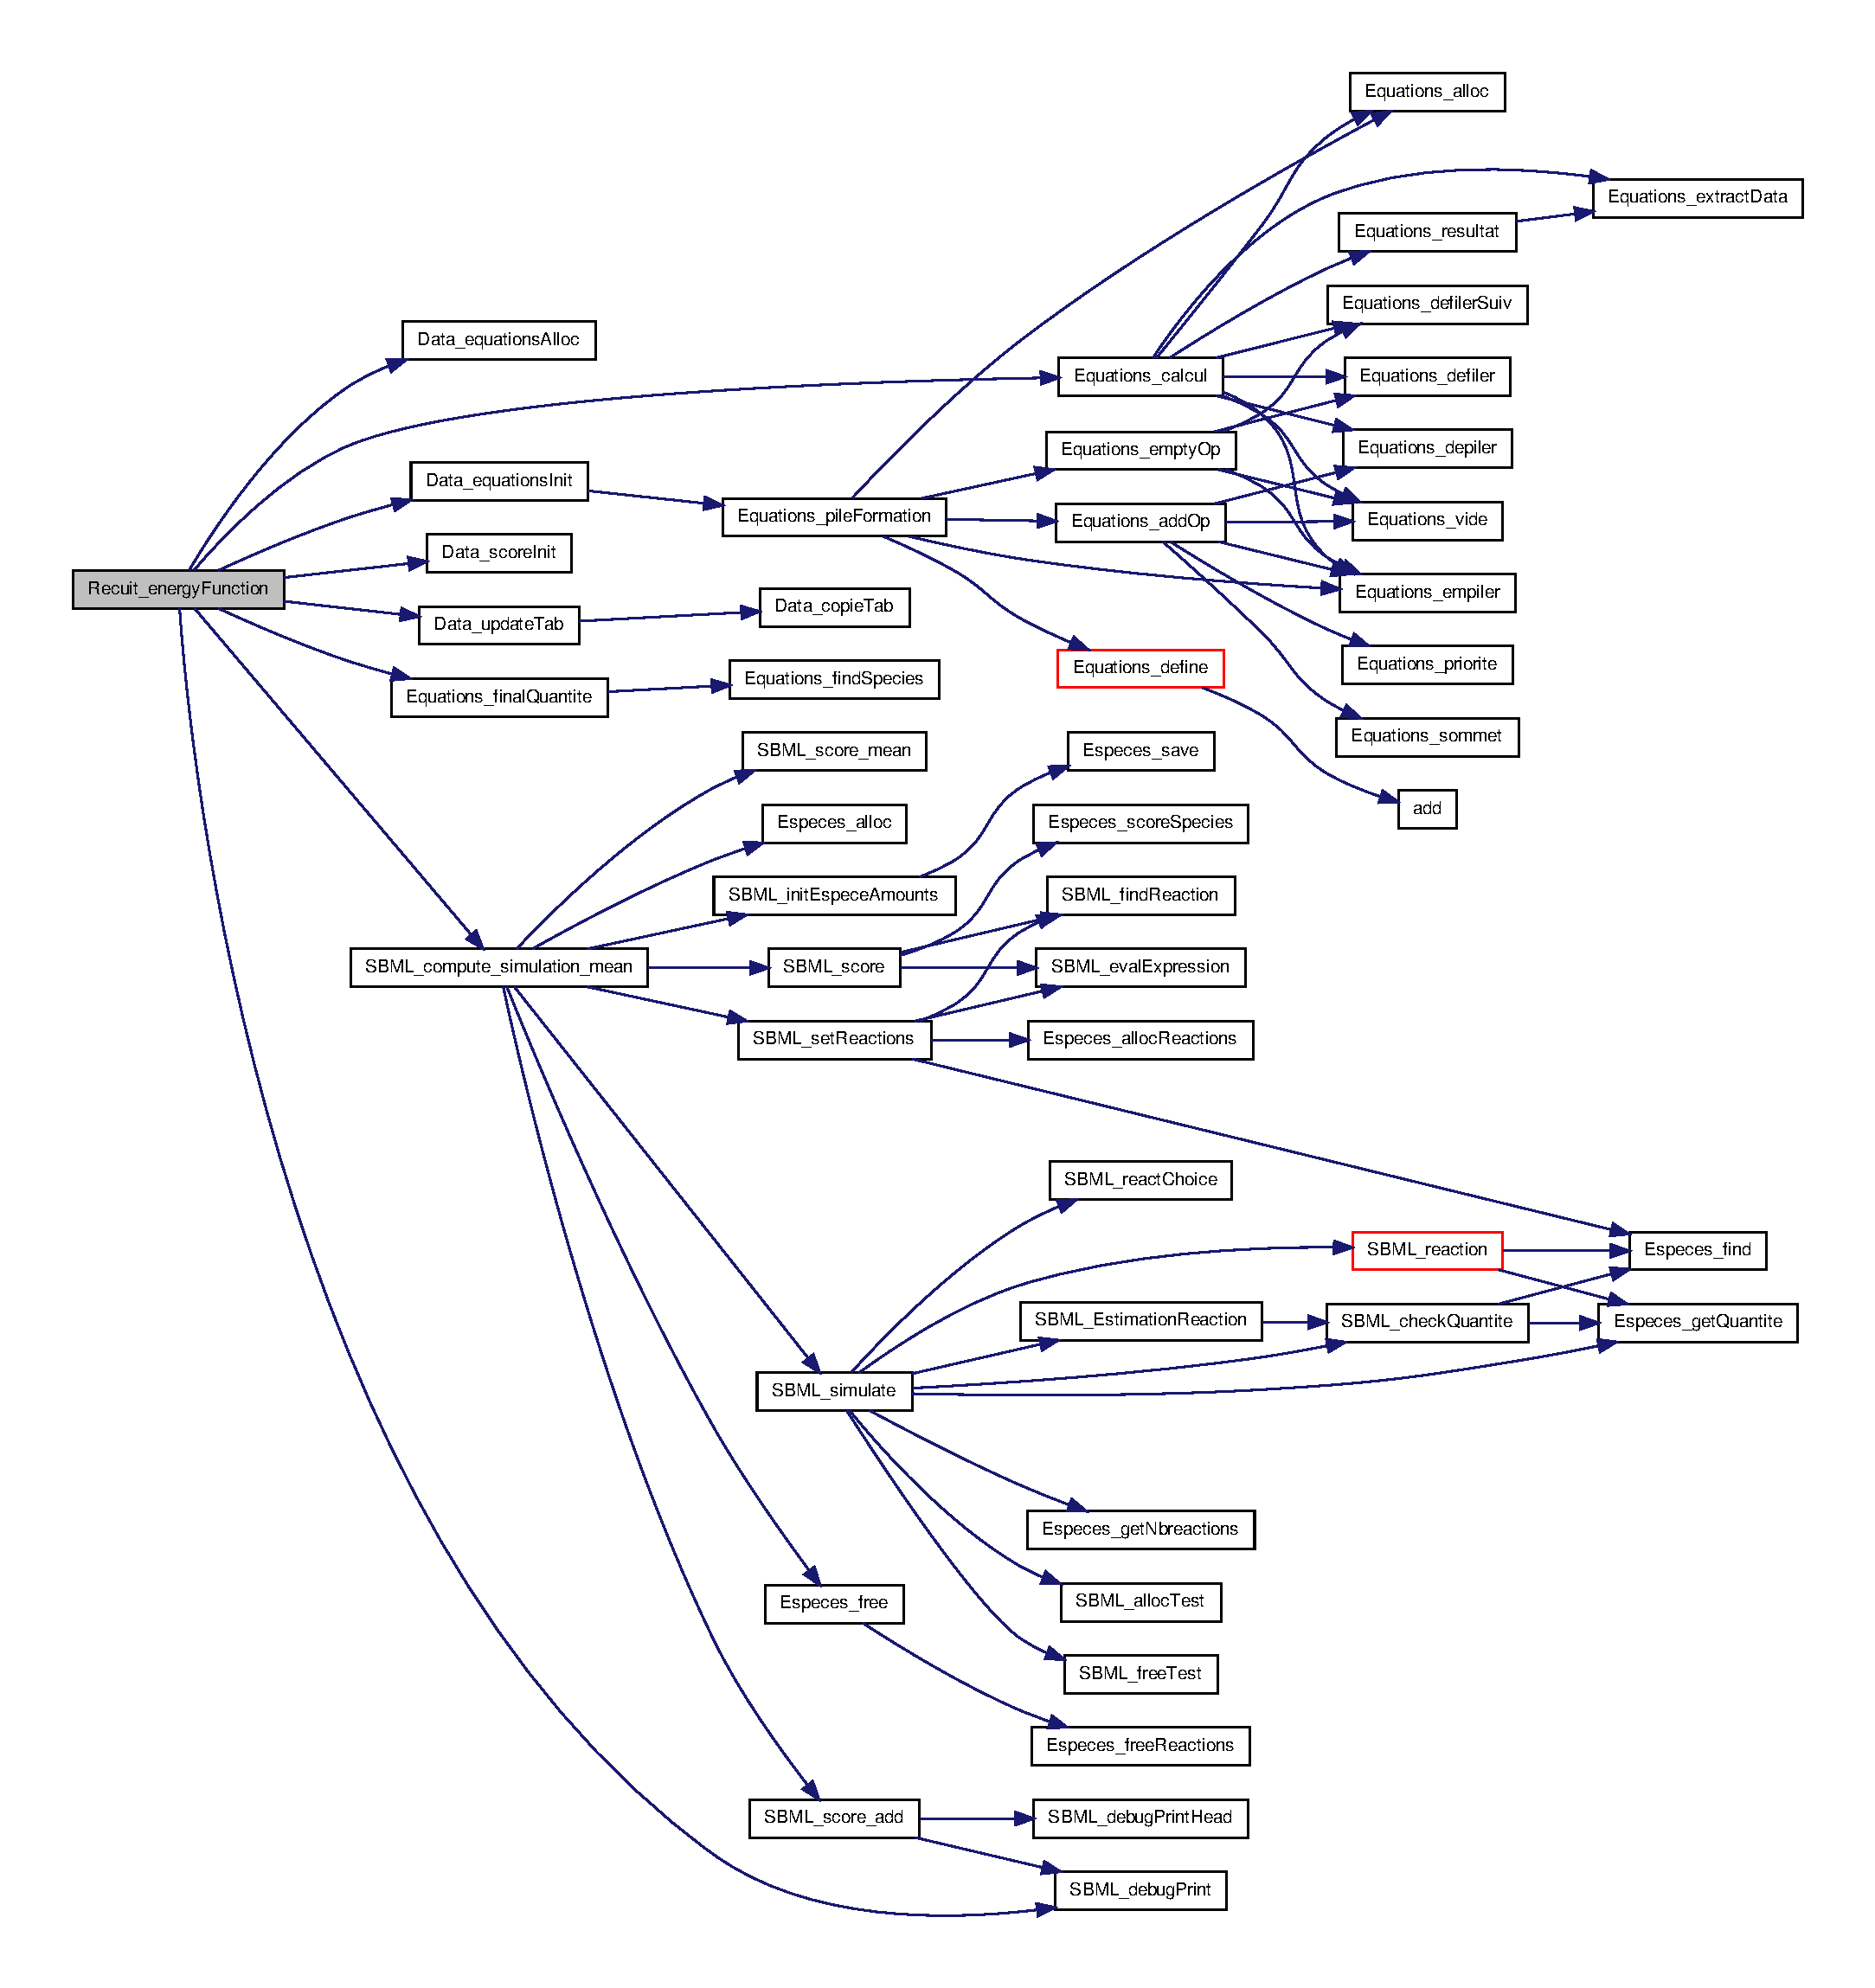
\includegraphics[width=400pt]{gsl__recuit_8h_a76e1fe1e0d6471f07f55bcf28d247fa5_cgraph}
\end{center}
\end{figure}


\hypertarget{gsl__recuit_8h_a262f0cba7cb59023d3b45bc17c103aac}{
\index{gsl\_\-recuit.h@{gsl\_\-recuit.h}!Recuit\_\-metricDistance@{Recuit\_\-metricDistance}}
\index{Recuit\_\-metricDistance@{Recuit\_\-metricDistance}!gsl_recuit.h@{gsl\_\-recuit.h}}
\subsubsection[{Recuit\_\-metricDistance}]{\setlength{\rightskip}{0pt plus 5cm}double Recuit\_\-metricDistance (
\begin{DoxyParamCaption}
\item[{void $\ast$}]{xp, }
\item[{void $\ast$}]{yp}
\end{DoxyParamCaption}
)}}
\label{gsl__recuit_8h_a262f0cba7cb59023d3b45bc17c103aac}


Compute the distance between the two table. 

\begin{DoxyAuthor}{Author}
Amine Ghozlane 
\end{DoxyAuthor}

\begin{DoxyParams}{Parameters}
{\em xp} & Past short table of reaction parameters \\
\hline
{\em yp} & New short table of reaction parameters \\
\hline
\end{DoxyParams}
\begin{DoxyReturn}{Returns}
Distance between the two table 
\end{DoxyReturn}


Definition at line 115 of file gsl\_\-recuit.c.



References ListParameters::interest\_\-parameters.



Referenced by Recuit\_\-compute\_\-recuit().

\hypertarget{gsl__recuit_8h_a41e47a5713188f196ebc7a66a9052d3d}{
\index{gsl\_\-recuit.h@{gsl\_\-recuit.h}!Recuit\_\-printParametre@{Recuit\_\-printParametre}}
\index{Recuit\_\-printParametre@{Recuit\_\-printParametre}!gsl_recuit.h@{gsl\_\-recuit.h}}
\subsubsection[{Recuit\_\-printParametre}]{\setlength{\rightskip}{0pt plus 5cm}void Recuit\_\-printParametre (
\begin{DoxyParamCaption}
\item[{double $\ast$}]{x\_\-initial}
\end{DoxyParamCaption}
)}}
\label{gsl__recuit_8h_a41e47a5713188f196ebc7a66a9052d3d}


Print initial parameters. 

\begin{DoxyAuthor}{Author}
Amine Ghozlane 
\end{DoxyAuthor}

\begin{DoxyParams}{Parameters}
{\em x\_\-initial} & table of reaction parameters \\
\hline
\end{DoxyParams}


Definition at line 279 of file gsl\_\-recuit.c.



References ListParameters::conf, ListParameters::interest\_\-parameters, Xml\_\-getBoltzmann(), Xml\_\-getMuT(), Xml\_\-getNbIters(), Xml\_\-getNbTriesSa(), Xml\_\-getStepSize(), Xml\_\-getTinitial(), and Xml\_\-getTmin().



Referenced by Recuit\_\-compute\_\-recuit().



Here is the call graph for this function:\nopagebreak
\begin{figure}[H]
\begin{center}
\leavevmode
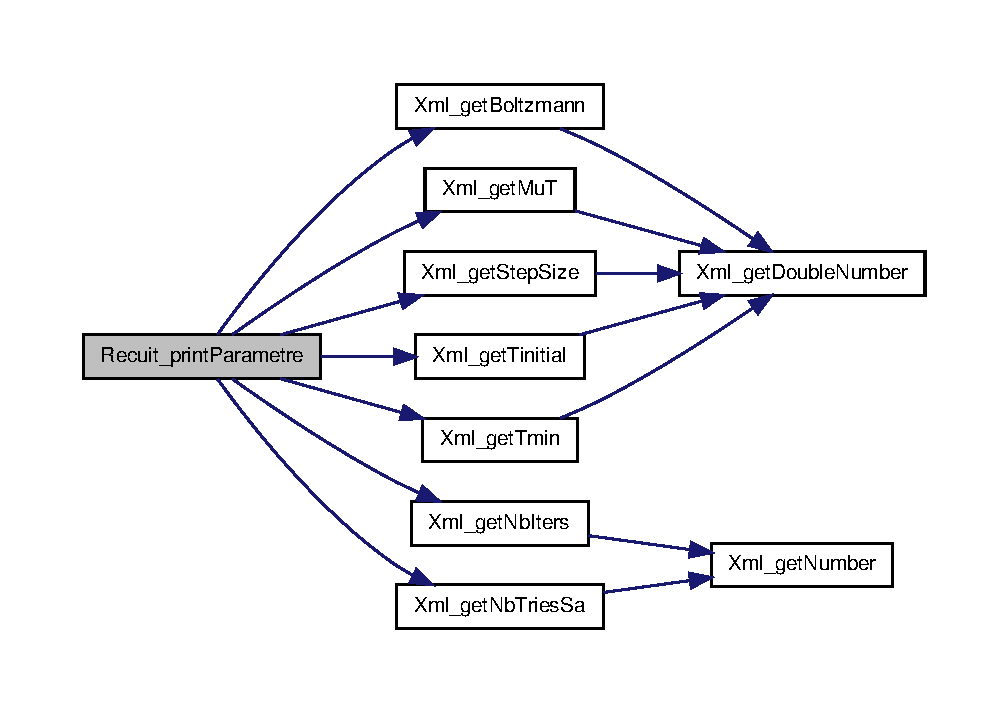
\includegraphics[width=400pt]{gsl__recuit_8h_a41e47a5713188f196ebc7a66a9052d3d_cgraph}
\end{center}
\end{figure}


\hypertarget{gsl__recuit_8h_afd9db376bfecbe387f3836854c31f6d0}{
\index{gsl\_\-recuit.h@{gsl\_\-recuit.h}!Recuit\_\-printPosition@{Recuit\_\-printPosition}}
\index{Recuit\_\-printPosition@{Recuit\_\-printPosition}!gsl_recuit.h@{gsl\_\-recuit.h}}
\subsubsection[{Recuit\_\-printPosition}]{\setlength{\rightskip}{0pt plus 5cm}void Recuit\_\-printPosition (
\begin{DoxyParamCaption}
\item[{void $\ast$}]{xp}
\end{DoxyParamCaption}
)}}
\label{gsl__recuit_8h_afd9db376bfecbe387f3836854c31f6d0}


Print the table of reaction parameters. 

\begin{DoxyAuthor}{Author}
Amine Ghozlane 
\end{DoxyAuthor}

\begin{DoxyParams}{Parameters}
{\em xp} & Short table of reaction parameters \\
\hline
\end{DoxyParams}


Definition at line 158 of file gsl\_\-recuit.c.



References Data\_\-updateTab(), ListParameters::nb\_\-parameters, and SimParameters::y.



Referenced by Recuit\_\-compute\_\-recuit().



Here is the call graph for this function:\nopagebreak
\begin{figure}[H]
\begin{center}
\leavevmode
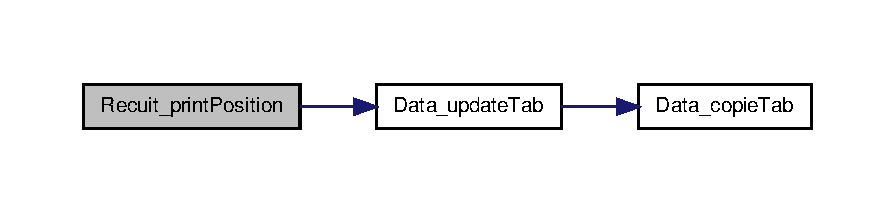
\includegraphics[width=400pt]{gsl__recuit_8h_afd9db376bfecbe387f3836854c31f6d0_cgraph}
\end{center}
\end{figure}


\hypertarget{gsl__recuit_8h_a50384383f4c2a13a1f7dc85f69339bd6}{
\index{gsl\_\-recuit.h@{gsl\_\-recuit.h}!Recuit\_\-redirectionFlux@{Recuit\_\-redirectionFlux}}
\index{Recuit\_\-redirectionFlux@{Recuit\_\-redirectionFlux}!gsl_recuit.h@{gsl\_\-recuit.h}}
\subsubsection[{Recuit\_\-redirectionFlux}]{\setlength{\rightskip}{0pt plus 5cm}FILE$\ast$ Recuit\_\-redirectionFlux (
\begin{DoxyParamCaption}
\item[{{\bf xmlConfig\_\-t} $\ast$}]{conf, }
\item[{FILE $\ast$}]{f, }
\item[{char $\ast$$\ast$}]{files\_\-path, }
\item[{int}]{number}
\end{DoxyParamCaption}
)}}
\label{gsl__recuit_8h_a50384383f4c2a13a1f7dc85f69339bd6}


Redirect stdout flux. 

\begin{DoxyAuthor}{Author}
Amine Ghozlane 
\end{DoxyAuthor}

\begin{DoxyParams}{Parameters}
{\em conf} & Struct \hyperlink{structxmlConfig__t}{xmlConfig\_\-t} \\
\hline
{\em f} & File name \\
\hline
{\em files\_\-path} & List of paths \\
\hline
{\em number} & Index of out repertory \\
\hline
\end{DoxyParams}
\begin{DoxyReturn}{Returns}
Out flux 
\end{DoxyReturn}


Definition at line 184 of file gsl\_\-recuit.c.



References Xml\_\-getString().



Referenced by Recuit\_\-compute\_\-recuit().



Here is the call graph for this function:\nopagebreak
\begin{figure}[H]
\begin{center}
\leavevmode
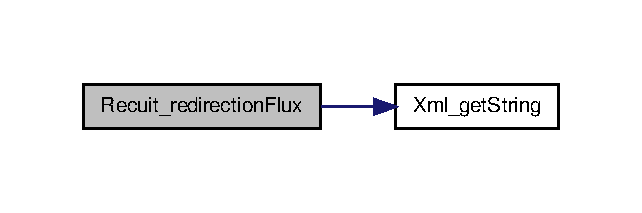
\includegraphics[width=308pt]{gsl__recuit_8h_a50384383f4c2a13a1f7dc85f69339bd6_cgraph}
\end{center}
\end{figure}


\hypertarget{gsl__recuit_8h_a992371555f490f726cbe4a1c90785a09}{
\index{gsl\_\-recuit.h@{gsl\_\-recuit.h}!Recuit\_\-takeStep@{Recuit\_\-takeStep}}
\index{Recuit\_\-takeStep@{Recuit\_\-takeStep}!gsl_recuit.h@{gsl\_\-recuit.h}}
\subsubsection[{Recuit\_\-takeStep}]{\setlength{\rightskip}{0pt plus 5cm}void Recuit\_\-takeStep (
\begin{DoxyParamCaption}
\item[{const gsl\_\-rng $\ast$}]{r, }
\item[{void $\ast$}]{xp, }
\item[{double}]{step\_\-size}
\end{DoxyParamCaption}
)}}
\label{gsl__recuit_8h_a992371555f490f726cbe4a1c90785a09}


Take a step through the solution space TSP. 

\begin{DoxyAuthor}{Author}
Amine Ghozlane 
\end{DoxyAuthor}

\begin{DoxyParams}{Parameters}
{\em r} & Random number generator \\
\hline
{\em xp} & Short table of reaction parameters \\
\hline
{\em step\_\-size} & Size of step \\
\hline
\end{DoxyParams}


Definition at line 136 of file gsl\_\-recuit.c.



References ListParameters::interest\_\-parameters, ListParameters::nb\_\-couples, ListParameters::parameters, and Recuit\_\-verifParameters\_\-2().



Referenced by Recuit\_\-compute\_\-recuit().



Here is the call graph for this function:\nopagebreak
\begin{figure}[H]
\begin{center}
\leavevmode
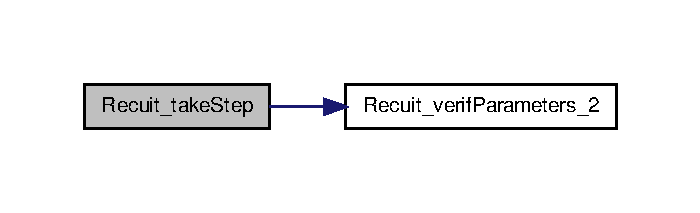
\includegraphics[width=336pt]{gsl__recuit_8h_a992371555f490f726cbe4a1c90785a09_cgraph}
\end{center}
\end{figure}


\hypertarget{gsl__recuit_8h_acc458cd24422d89b326a1b4bb7940cbf}{
\index{gsl\_\-recuit.h@{gsl\_\-recuit.h}!Recuit\_\-verifParameters@{Recuit\_\-verifParameters}}
\index{Recuit\_\-verifParameters@{Recuit\_\-verifParameters}!gsl_recuit.h@{gsl\_\-recuit.h}}
\subsubsection[{Recuit\_\-verifParameters}]{\setlength{\rightskip}{0pt plus 5cm}void Recuit\_\-verifParameters (
\begin{DoxyParamCaption}
\item[{double $\ast$}]{x\_\-initial, }
\item[{const gsl\_\-rng $\ast$}]{r, }
\item[{int}]{debut, }
\item[{int}]{max}
\end{DoxyParamCaption}
)}}
\label{gsl__recuit_8h_acc458cd24422d89b326a1b4bb7940cbf}


Choice of parameters and verification of their value. 

\begin{DoxyAuthor}{Author}
Amine Ghozlane 
\end{DoxyAuthor}

\begin{DoxyParams}{Parameters}
{\em x\_\-initial} & table of reaction parameters \\
\hline
{\em r} & Random number generator \\
\hline
{\em debut} & Beginning \\
\hline
{\em max} & End \\
\hline
\end{DoxyParams}


Definition at line 207 of file gsl\_\-recuit.c.



Referenced by Recuit\_\-defParametre().

\hypertarget{gsl__recuit_8h_a389f2f70421b758b2eaea08d8ef9033a}{
\index{gsl\_\-recuit.h@{gsl\_\-recuit.h}!Recuit\_\-verifParameters\_\-2@{Recuit\_\-verifParameters\_\-2}}
\index{Recuit\_\-verifParameters\_\-2@{Recuit\_\-verifParameters\_\-2}!gsl_recuit.h@{gsl\_\-recuit.h}}
\subsubsection[{Recuit\_\-verifParameters\_\-2}]{\setlength{\rightskip}{0pt plus 5cm}void Recuit\_\-verifParameters\_\-2 (
\begin{DoxyParamCaption}
\item[{double $\ast$}]{new\_\-x, }
\item[{double $\ast$}]{old\_\-x, }
\item[{const gsl\_\-rng $\ast$}]{r, }
\item[{int}]{debut, }
\item[{int}]{max, }
\item[{double}]{step\_\-size}
\end{DoxyParamCaption}
)}}
\label{gsl__recuit_8h_a389f2f70421b758b2eaea08d8ef9033a}


Choice of parameters and verification of their value. 

\begin{DoxyAuthor}{Author}
Amine Ghozlane 
\end{DoxyAuthor}

\begin{DoxyParams}{Parameters}
{\em new\_\-x} & table of reaction parameters \\
\hline
{\em old\_\-x} & table of reaction parameters \\
\hline
{\em r} & Random number generator \\
\hline
{\em debut} & Beginning \\
\hline
{\em max} & End \\
\hline
{\em step\_\-size} & Size of the step \\
\hline
\end{DoxyParams}


Definition at line 235 of file gsl\_\-recuit.c.



Referenced by Recuit\_\-takeStep().


\hypertarget{gsl__sd_8h}{
\section{metaboflux/include/gsl\_\-sd.h File Reference}
\label{gsl__sd_8h}\index{metaboflux/include/gsl\_\-sd.h@{metaboflux/include/gsl\_\-sd.h}}
}


Compute the standard deviation analysis of the simulations.  


This graph shows which files directly or indirectly include this file:\nopagebreak
\begin{figure}[H]
\begin{center}
\leavevmode
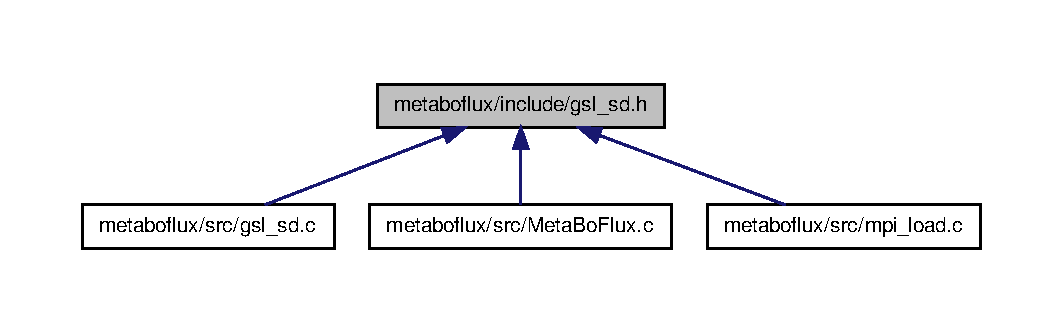
\includegraphics[width=400pt]{gsl__sd_8h__dep__incl}
\end{center}
\end{figure}
\subsection*{Functions}
\begin{DoxyCompactItemize}
\item 
double \hyperlink{gsl__sd_8h_a8e6c5bf8137775f39959114bc6180898}{Sd\_\-compute\_\-simulation} (\hyperlink{structListParameters}{pListParameters}, \hyperlink{structSimParameters}{pSimParameters})
\begin{DoxyCompactList}\small\item\em Enter in the program for standard deviation. \end{DoxyCompactList}\item 
void \hyperlink{gsl__sd_8h_a3574b473c8bc4f17b1d3921621f78132}{Sd\_\-compute\_\-standard\_\-deviation} (\hyperlink{structListParameters}{pListParameters}, double $\ast$, double $\ast$, char $\ast$$\ast$, int, int)
\begin{DoxyCompactList}\small\item\em Compute the standard deviation. \end{DoxyCompactList}\end{DoxyCompactItemize}


\subsection{Detailed Description}
Compute the standard deviation analysis of the simulations. This file is part of MetaBoFlux (\href{http://www.cbib.u-bordeaux2.fr/metaboflux/}{\tt http://www.cbib.u-\/bordeaux2.fr/metaboflux/}) Copyright (C) 2010 Amine Ghozlane from LaBRI and University of Bordeaux 1

MetaBoFlux is free software: you can redistribute it and/or modify it under the terms of the GNU Lesser General Public License as published by the Free Software Foundation, either version 3 of the License, or (at your option) any later version.

MetaBoFlux is distributed in the hope that it will be useful, but WITHOUT ANY WARRANTY; without even the implied warranty of MERCHANTABILITY or FITNESS FOR A PARTICULAR PURPOSE. See the GNU General Public License for more details.

You should have received a copy of the GNU Lesser General Public License along with this program. If not, see $<$\href{http://www.gnu.org/licenses/}{\tt http://www.gnu.org/licenses/}$>$.

\begin{DoxyAuthor}{Author}
\{Amine Ghozlane\} 
\end{DoxyAuthor}
\begin{DoxyVersion}{Version}
2.0 
\end{DoxyVersion}
\begin{DoxyDate}{Date}
9 novembre 2009 
\end{DoxyDate}


Definition in file \hyperlink{gsl__sd_8h_source}{gsl\_\-sd.h}.



\subsection{Function Documentation}
\hypertarget{gsl__sd_8h_a8e6c5bf8137775f39959114bc6180898}{
\index{gsl\_\-sd.h@{gsl\_\-sd.h}!Sd\_\-compute\_\-simulation@{Sd\_\-compute\_\-simulation}}
\index{Sd\_\-compute\_\-simulation@{Sd\_\-compute\_\-simulation}!gsl_sd.h@{gsl\_\-sd.h}}
\subsubsection[{Sd\_\-compute\_\-simulation}]{\setlength{\rightskip}{0pt plus 5cm}double Sd\_\-compute\_\-simulation (
\begin{DoxyParamCaption}
\item[{{\bf pListParameters}}]{all, }
\item[{{\bf pSimParameters}}]{sim}
\end{DoxyParamCaption}
)}}
\label{gsl__sd_8h_a8e6c5bf8137775f39959114bc6180898}


Enter in the program for standard deviation. 

\begin{DoxyAuthor}{Author}
Amine Ghozlane 
\end{DoxyAuthor}

\begin{DoxyParams}{Parameters}
{\em all} & Global parameters : struct \hyperlink{structListParameters}{ListParameters} \\
\hline
{\em sim} & Simulation parameters : struct \hyperlink{structSimParameters}{SimParameters} \\
\hline
\end{DoxyParams}
\begin{DoxyReturn}{Returns}
Energy value 
\end{DoxyReturn}


Definition at line 56 of file gsl\_\-sd.c.



References ListParameters::banned, Data\_\-equationsAlloc(), Data\_\-equationsInit(), Data\_\-scoreInit(), SimParameters::debugFile, Equations\_\-calcul(), Equations\_\-finalQuantite(), ListParameters::model, Score::name, ListParameters::nb\_\-banned, ListParameters::nb\_\-equations, Score::nb\_\-species, SimParameters::out, SimParameters::pile, Score::quantite, SimParameters::r, SBML\_\-compute\_\-simulation(), SBML\_\-debugPrint(), SBML\_\-debugPrintHead(), Score::species, Score::species\_\-amount, Score::species\_\-weight, Score::taille, Score::tailleSpecies, and SimParameters::y.



Referenced by Sd\_\-compute\_\-standard\_\-deviation().



Here is the call graph for this function:\nopagebreak
\begin{figure}[H]
\begin{center}
\leavevmode
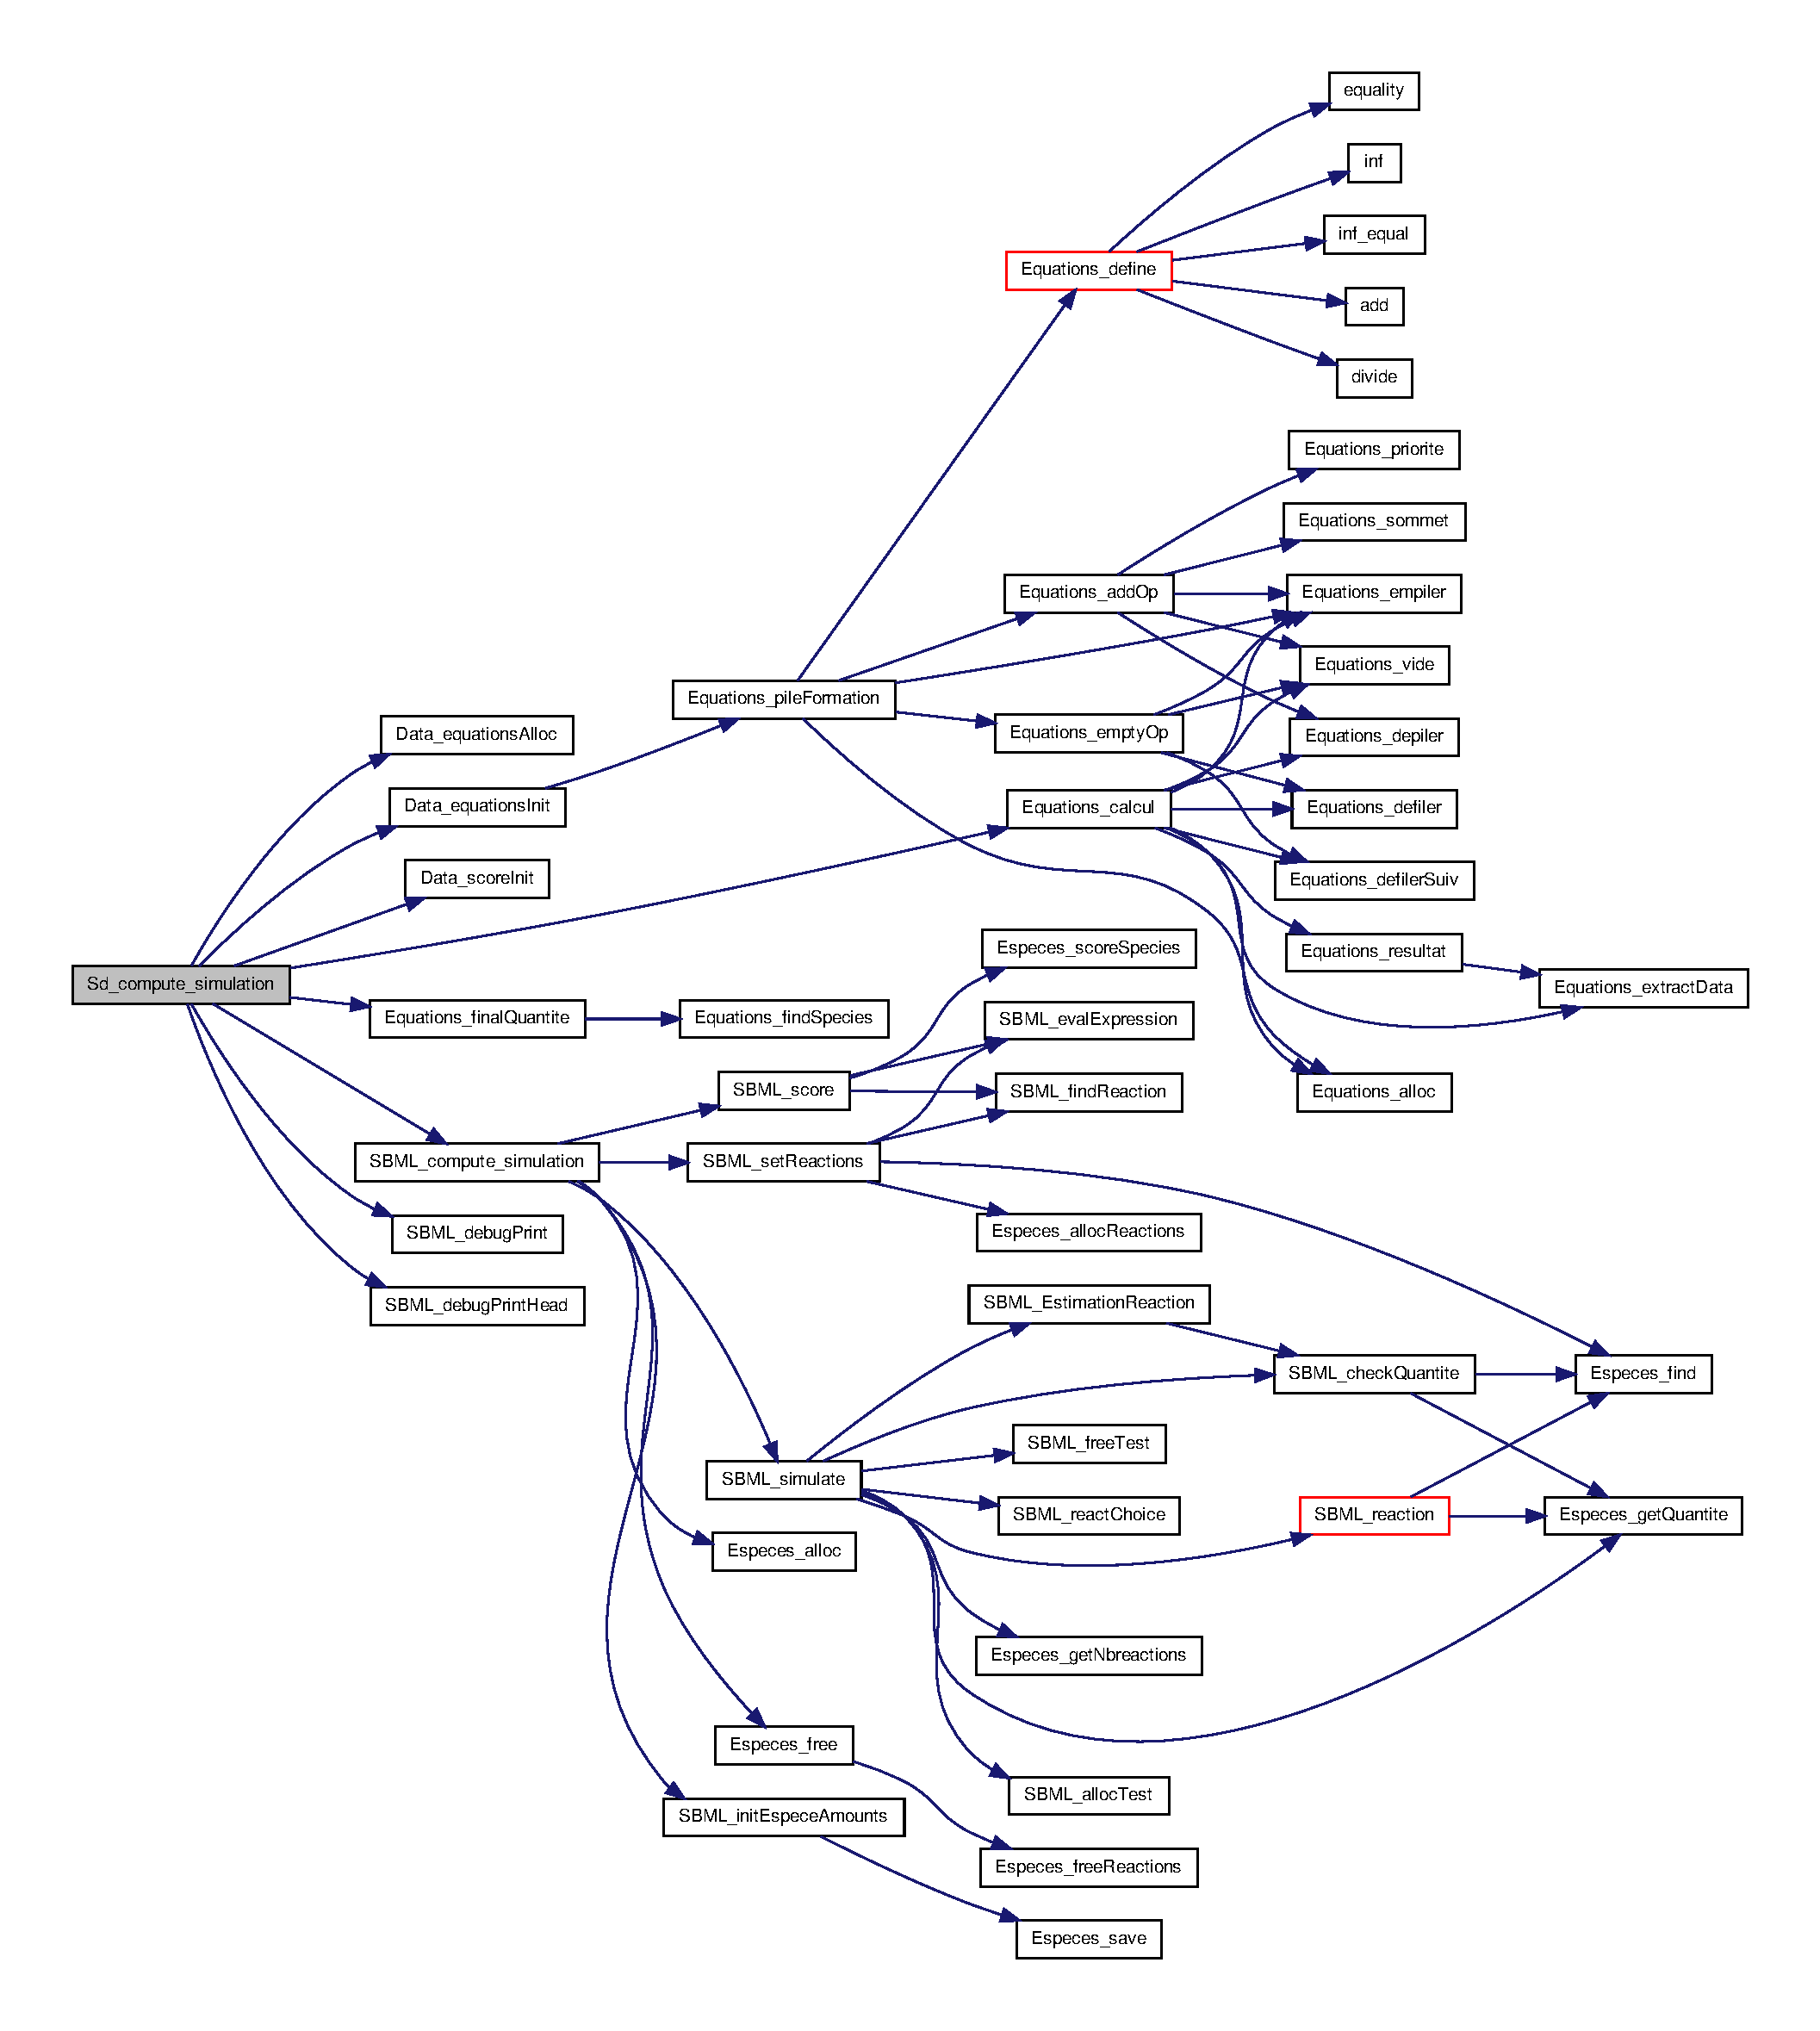
\includegraphics[width=400pt]{gsl__sd_8h_a8e6c5bf8137775f39959114bc6180898_cgraph}
\end{center}
\end{figure}


\hypertarget{gsl__sd_8h_a3574b473c8bc4f17b1d3921621f78132}{
\index{gsl\_\-sd.h@{gsl\_\-sd.h}!Sd\_\-compute\_\-standard\_\-deviation@{Sd\_\-compute\_\-standard\_\-deviation}}
\index{Sd\_\-compute\_\-standard\_\-deviation@{Sd\_\-compute\_\-standard\_\-deviation}!gsl_sd.h@{gsl\_\-sd.h}}
\subsubsection[{Sd\_\-compute\_\-standard\_\-deviation}]{\setlength{\rightskip}{0pt plus 5cm}void Sd\_\-compute\_\-standard\_\-deviation (
\begin{DoxyParamCaption}
\item[{{\bf pListParameters}}]{a, }
\item[{double $\ast$}]{fluxRatio, }
\item[{double $\ast$}]{result\_\-tab, }
\item[{char $\ast$$\ast$}]{files\_\-path, }
\item[{int}]{number\_\-arg, }
\item[{int}]{debug}
\end{DoxyParamCaption}
)}}
\label{gsl__sd_8h_a3574b473c8bc4f17b1d3921621f78132}


Compute the standard deviation. 

\begin{DoxyAuthor}{Author}
Amine Ghozlane 
\end{DoxyAuthor}

\begin{DoxyParams}{Parameters}
{\em a} & struct \hyperlink{structListParameters}{ListParameters} \\
\hline
{\em fluxRatio} & Ratio parameters \\
\hline
{\em result\_\-tab} & Result table \\
\hline
{\em files\_\-path} & List of paths \\
\hline
{\em number\_\-arg} & Number of simulation \\
\hline
{\em debug} & Debug flag \\
\hline
\end{DoxyParams}


Definition at line 106 of file gsl\_\-sd.c.



References ListParameters::conf, Data\_\-desallocSim(), Data\_\-simParameters(), ListParameters::nb\_\-parameters, Sd\_\-compute\_\-simulation(), Xml\_\-getNbTriesMod(), and SimParameters::y.



Referenced by Mpi\_\-slave().



Here is the call graph for this function:\nopagebreak
\begin{figure}[H]
\begin{center}
\leavevmode
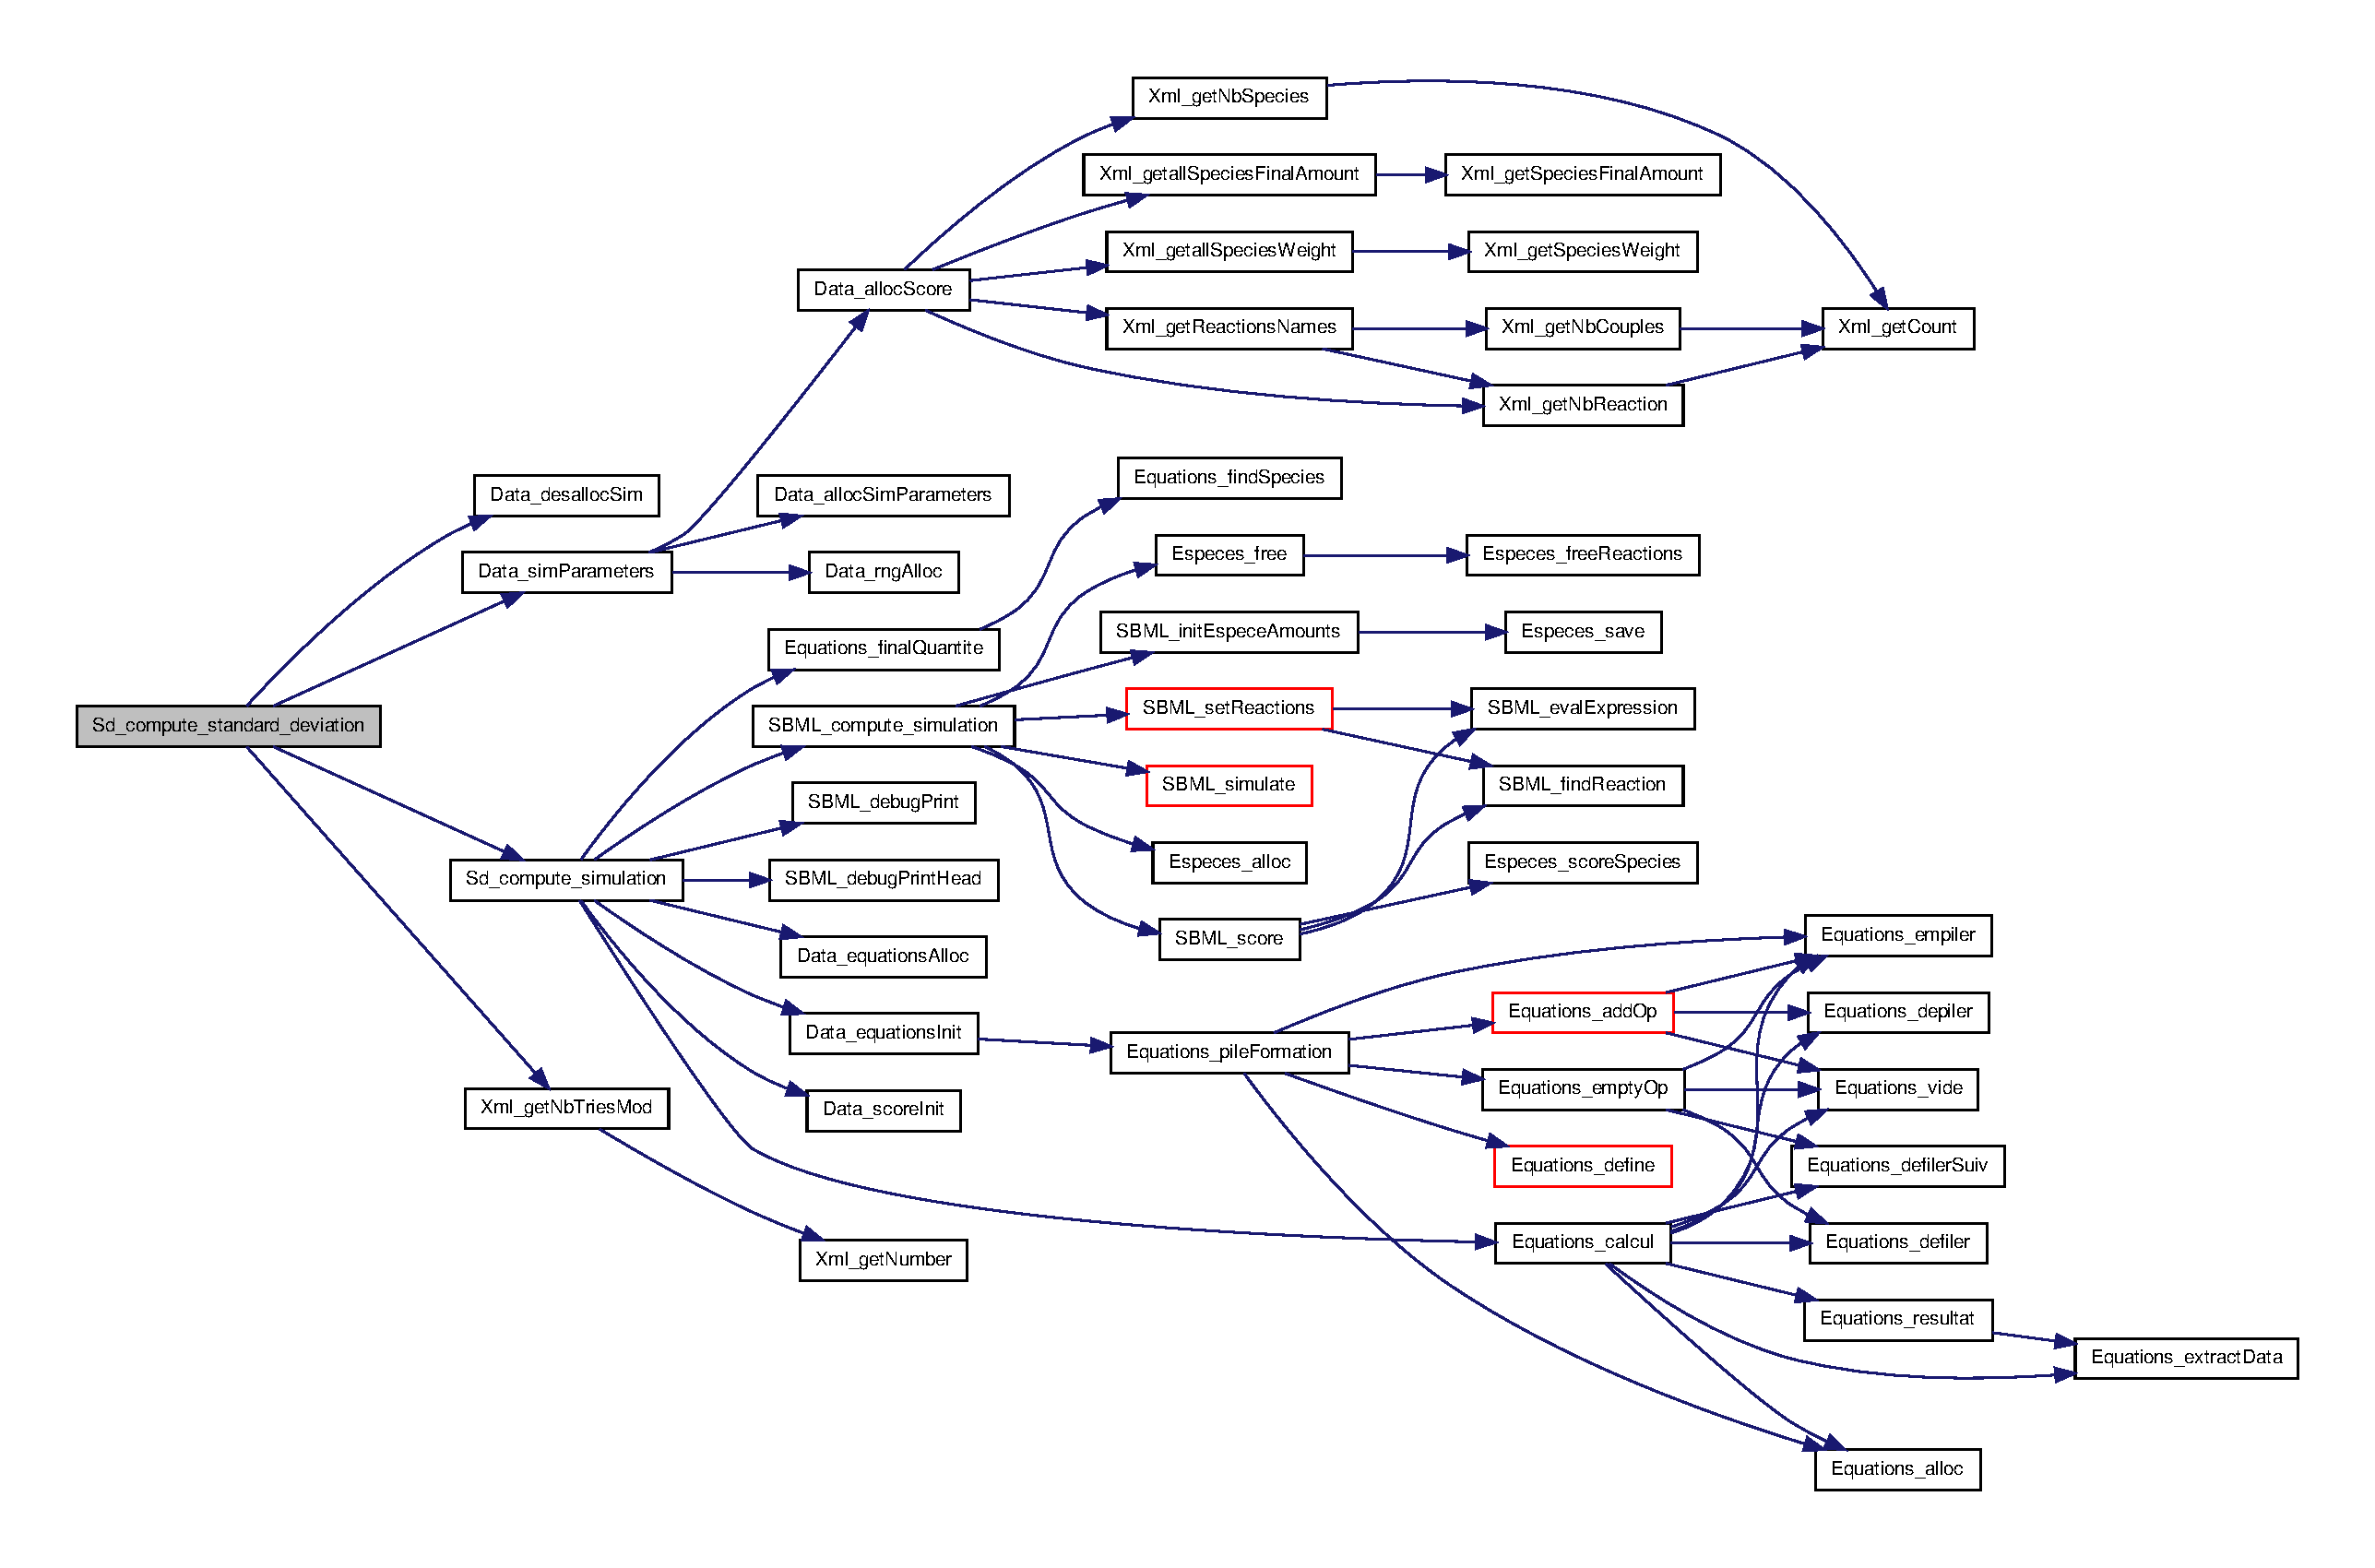
\includegraphics[width=400pt]{gsl__sd_8h_a3574b473c8bc4f17b1d3921621f78132_cgraph}
\end{center}
\end{figure}



\hypertarget{mpi__load_8h}{
\section{metaboflux/include/mpi\_\-load.h File Reference}
\label{mpi__load_8h}\index{metaboflux/include/mpi\_\-load.h@{metaboflux/include/mpi\_\-load.h}}
}


Parallelize the program.  


This graph shows which files directly or indirectly include this file:\nopagebreak
\begin{figure}[H]
\begin{center}
\leavevmode
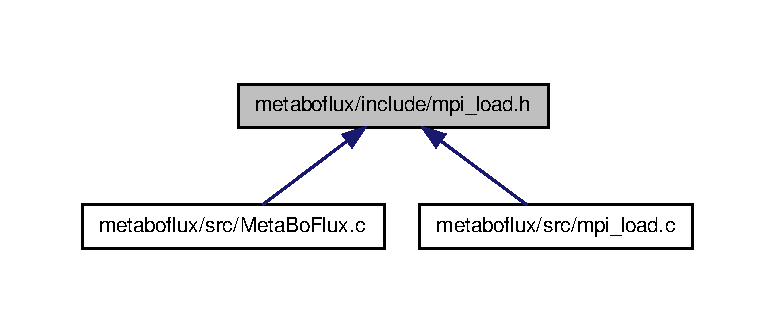
\includegraphics[width=372pt]{mpi__load_8h__dep__incl}
\end{center}
\end{figure}
\subsection*{Functions}
\begin{DoxyCompactItemize}
\item 
int \hyperlink{mpi__load_8h_afc95cdfc5153ccd5954a98aa7961a626}{Mpi\_\-connectInterface} (int)
\begin{DoxyCompactList}\small\item\em Enter in the program for standard deviation. \end{DoxyCompactList}\item 
void \hyperlink{mpi__load_8h_ad7fe2a9dd47b4a4353fe4a95e443969a}{Mpi\_\-disconnectInterface} (int)
\begin{DoxyCompactList}\small\item\em Disconnection to the interface. \end{DoxyCompactList}\item 
void \hyperlink{mpi__load_8h_aa10a38be940ec3edbe44b5b5108e5e87}{Mpi\_\-init} (int, char $\ast$$\ast$, int $\ast$)
\begin{DoxyCompactList}\small\item\em Enter in the program for standard deviation. \end{DoxyCompactList}\item 
void \hyperlink{mpi__load_8h_a49f24c98f9724a9d2d64bf3b41d7c101}{Mpi\_\-master} (\hyperlink{structListParameters}{pListParameters}, char $\ast$$\ast$, int, int, int, int, int)
\begin{DoxyCompactList}\small\item\em Master process. \end{DoxyCompactList}\item 
void \hyperlink{mpi__load_8h_a4cf3597a859457305000e2168f205993}{Mpi\_\-writer} (\hyperlink{structListParameters}{pListParameters}, char $\ast$$\ast$, int, int, int)
\begin{DoxyCompactList}\small\item\em Master process. \end{DoxyCompactList}\item 
int \hyperlink{mpi__load_8h_ab4d2e0de3a14f863a405bddfa625b8bd}{Mpi\_\-sizeResultTab} (\hyperlink{structListParameters}{pListParameters}, int, int, int)
\begin{DoxyCompactList}\small\item\em Determine the size of the result tab. \end{DoxyCompactList}\item 
double $\ast$ \hyperlink{mpi__load_8h_aa305e4bef7acf975da871190b8e3e1d2}{Mpi\_\-allocResultTab} (int)
\begin{DoxyCompactList}\small\item\em Allocate the result tab. \end{DoxyCompactList}\item 
void \hyperlink{mpi__load_8h_aa753112f6c21ff66c1c63f511ccbb325}{Mpi\_\-writeSimFile} (\hyperlink{structListParameters}{pListParameters}, FILE $\ast$, FILE $\ast$, double $\ast$, int, int, int)
\begin{DoxyCompactList}\small\item\em Determine the size of the result tab. \end{DoxyCompactList}\item 
void \hyperlink{mpi__load_8h_a3f0c05e595da1760ed46a5f5f978a704}{Mpi\_\-writeSdFile} (FILE $\ast$, double $\ast$, int)
\begin{DoxyCompactList}\small\item\em Determine the size of the result tab. \end{DoxyCompactList}\item 
void \hyperlink{mpi__load_8h_a73a3042b31e240b5785eed805f963212}{Mpi\_\-slave} (\hyperlink{structListParameters}{pListParameters}, char $\ast$$\ast$, int, int, int)
\item 
void \hyperlink{mpi__load_8h_a68f6a4d5212d2eb5e853f8ab5d3f0f97}{Mpi\_\-finalize} (void)
\begin{DoxyCompactList}\small\item\em End MPI execution environment. \end{DoxyCompactList}\item 
void \hyperlink{mpi__load_8h_afeea8538ec6091c216e0d58a4b4ac9f1}{compute\_\-mpi} (int, char $\ast$$\ast$, char $\ast$$\ast$, int, int, int, int)
\begin{DoxyCompactList}\small\item\em Compute the simulated annealing through mpi. \end{DoxyCompactList}\end{DoxyCompactItemize}


\subsection{Detailed Description}
Parallelize the program. This file is part of MetaBoFlux (\href{http://www.cbib.u-bordeaux2.fr/metaboflux/}{\tt http://www.cbib.u-\/bordeaux2.fr/metaboflux/}) Copyright (C) 2010 Amine Ghozlane from LaBRI and University of Bordeaux 1

MetaBoFlux is free software: you can redistribute it and/or modify it under the terms of the GNU Lesser General Public License as published by the Free Software Foundation, either version 3 of the License, or (at your option) any later version.

MetaBoFlux is distributed in the hope that it will be useful, but WITHOUT ANY WARRANTY; without even the implied warranty of MERCHANTABILITY or FITNESS FOR A PARTICULAR PURPOSE. See the GNU General Public License for more details.

You should have received a copy of the GNU Lesser General Public License along with this program. If not, see $<$\href{http://www.gnu.org/licenses/}{\tt http://www.gnu.org/licenses/}$>$.

\begin{DoxyAuthor}{Author}
\{Amine Ghozlane\} 
\end{DoxyAuthor}
\begin{DoxyVersion}{Version}
2.0 
\end{DoxyVersion}
\begin{DoxyDate}{Date}
9 novembre 2009 
\end{DoxyDate}


Definition in file \hyperlink{mpi__load_8h_source}{mpi\_\-load.h}.



\subsection{Function Documentation}
\hypertarget{mpi__load_8h_afeea8538ec6091c216e0d58a4b4ac9f1}{
\index{mpi\_\-load.h@{mpi\_\-load.h}!compute\_\-mpi@{compute\_\-mpi}}
\index{compute\_\-mpi@{compute\_\-mpi}!mpi_load.h@{mpi\_\-load.h}}
\subsubsection[{compute\_\-mpi}]{\setlength{\rightskip}{0pt plus 5cm}void compute\_\-mpi (
\begin{DoxyParamCaption}
\item[{int}]{argc, }
\item[{char $\ast$$\ast$}]{argv, }
\item[{char $\ast$$\ast$}]{files\_\-path, }
\item[{int}]{activity, }
\item[{int}]{group, }
\item[{int}]{debug, }
\item[{int}]{port}
\end{DoxyParamCaption}
)}}
\label{mpi__load_8h_afeea8538ec6091c216e0d58a4b4ac9f1}


Compute the simulated annealing through mpi. 

\begin{DoxyAuthor}{Author}
Amine Ghozlane 
\end{DoxyAuthor}

\begin{DoxyParams}{Parameters}
{\em argc} & Number of arguments \\
\hline
{\em argv} & List of arguments \\
\hline
{\em files\_\-path} & List of paths \\
\hline
{\em activity} & Chosen activity \\
\hline
{\em group} & Group flag \\
\hline
{\em debug} & Debug flag \\
\hline
{\em port} & Interface port \\
\hline
\end{DoxyParams}


Definition at line 546 of file mpi\_\-load.c.



References Data\_\-desallocation(), Data\_\-parameters(), Mpi\_\-connectInterface(), Mpi\_\-disconnectInterface(), Mpi\_\-finalize(), Mpi\_\-init(), Mpi\_\-master(), Mpi\_\-slave(), and Mpi\_\-writer().



Referenced by main().



Here is the call graph for this function:\nopagebreak
\begin{figure}[H]
\begin{center}
\leavevmode
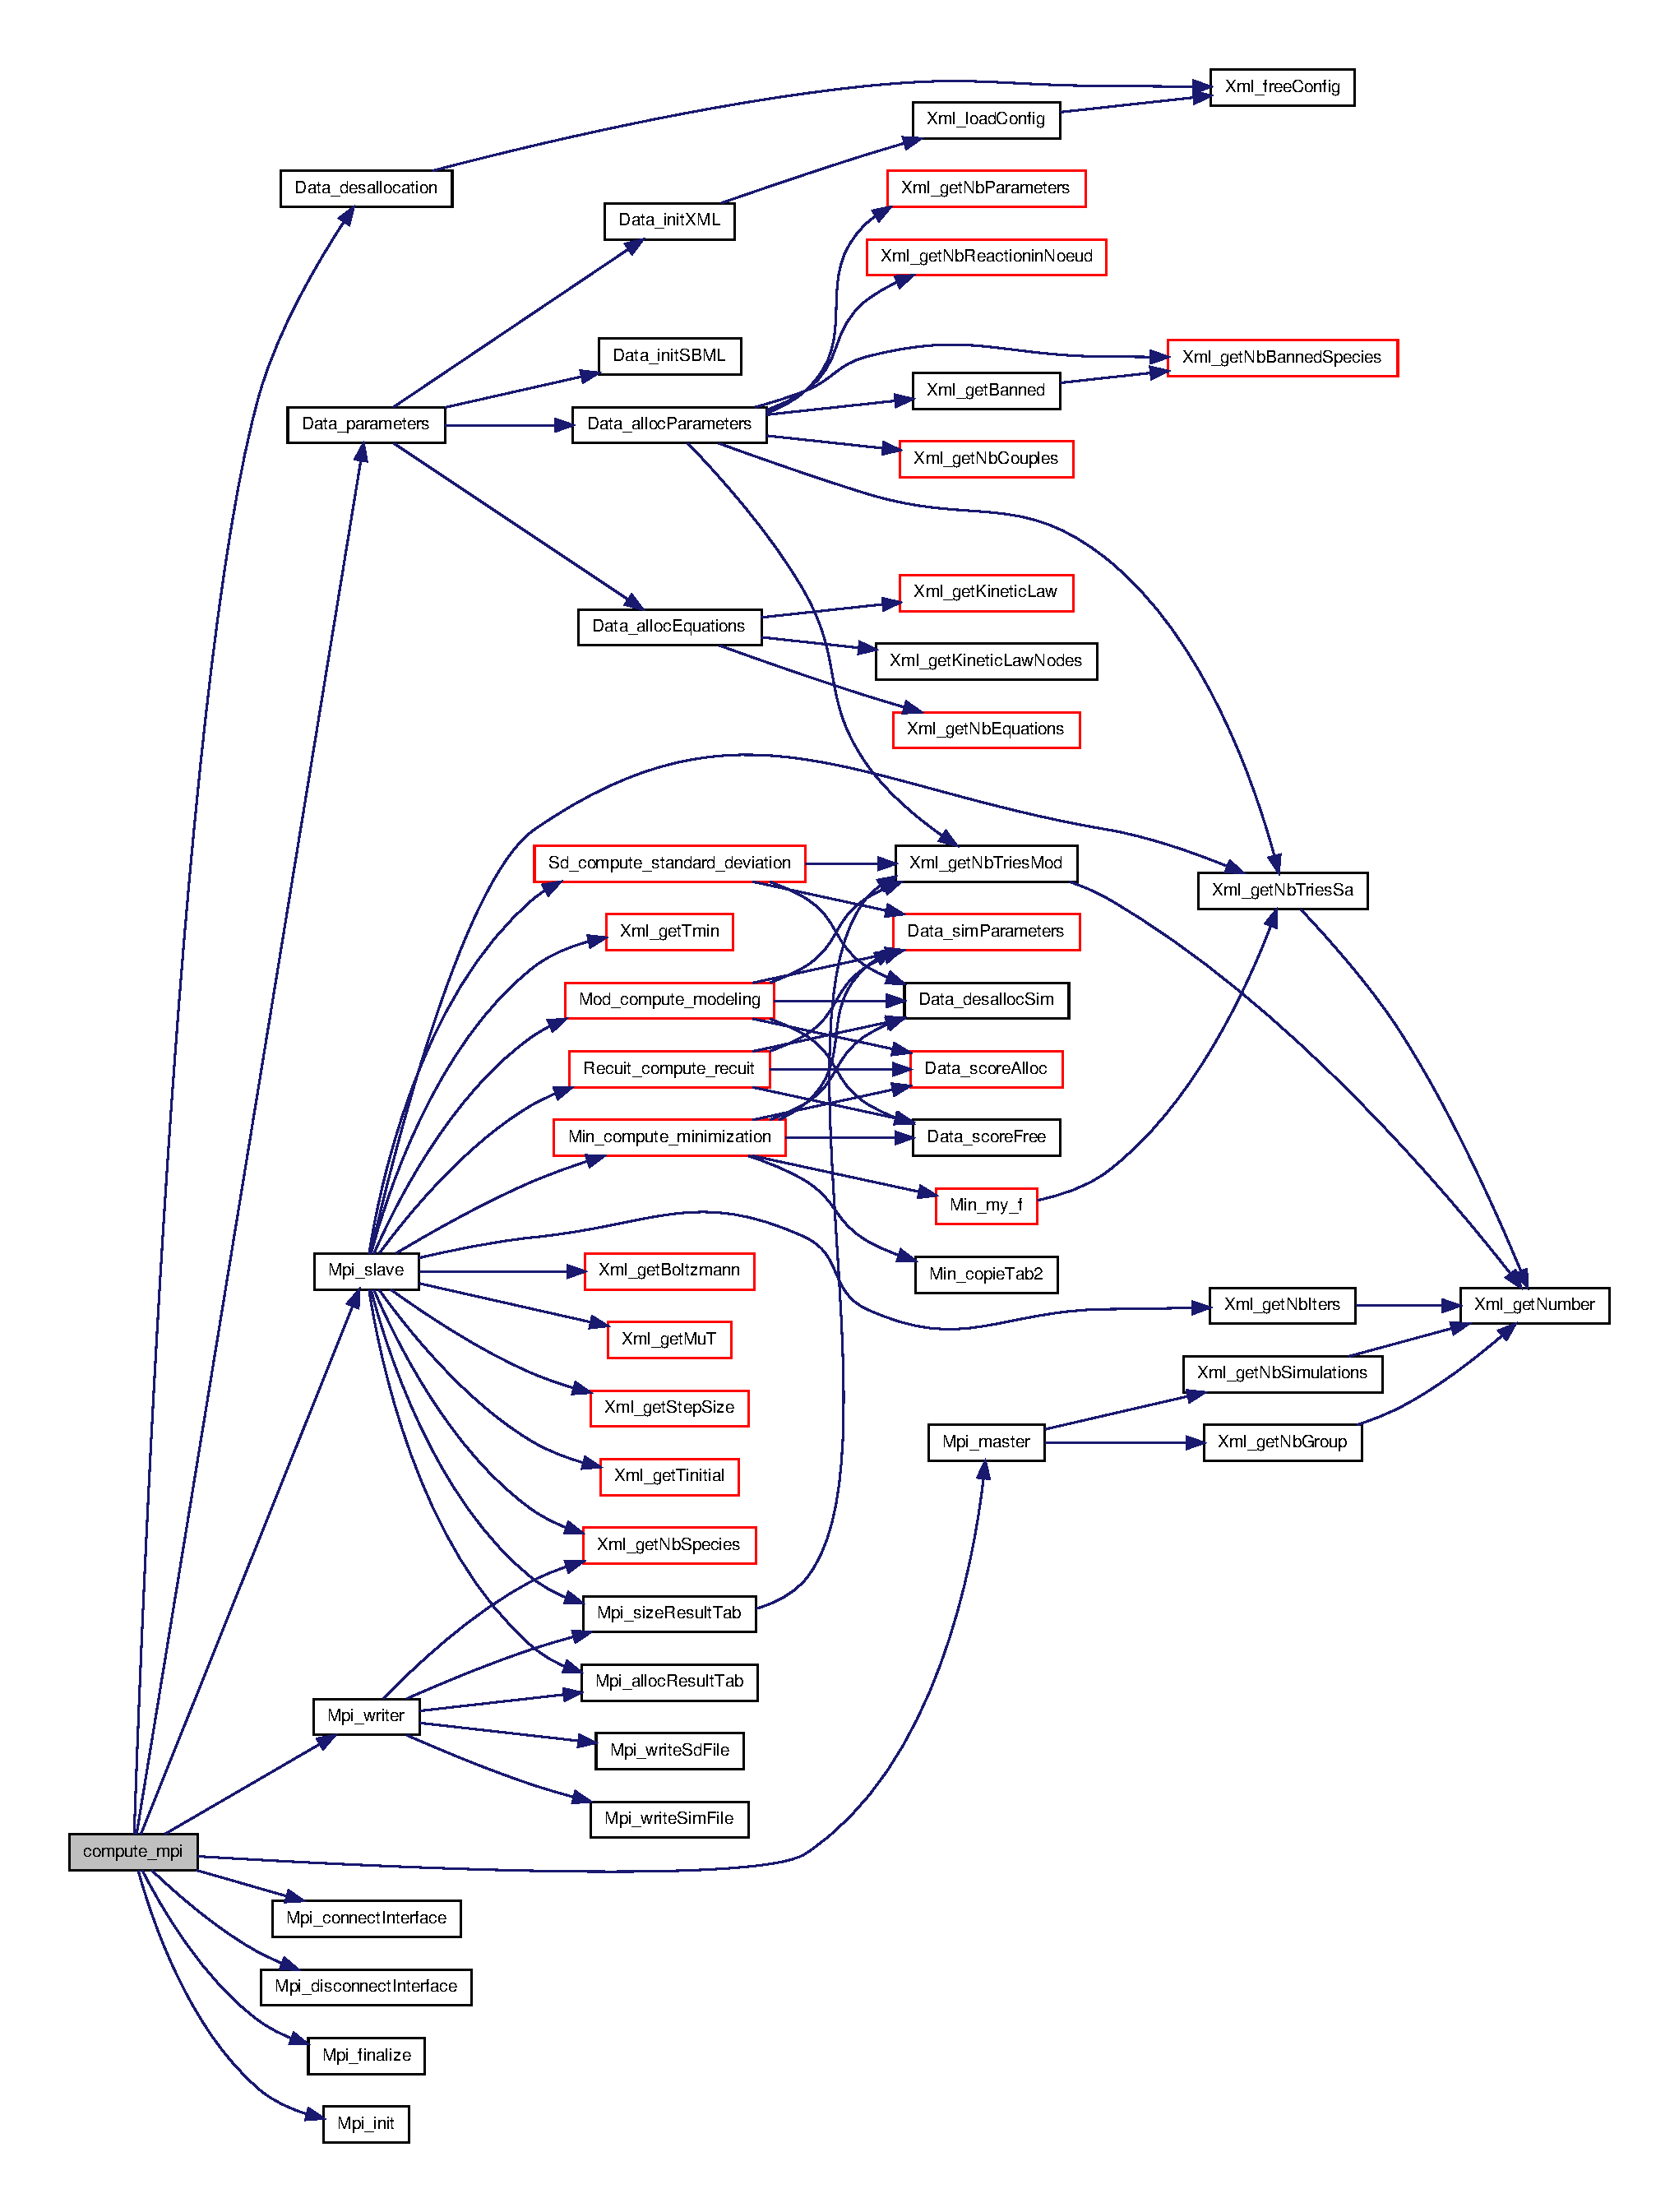
\includegraphics[width=400pt]{mpi__load_8h_afeea8538ec6091c216e0d58a4b4ac9f1_cgraph}
\end{center}
\end{figure}


\hypertarget{mpi__load_8h_aa305e4bef7acf975da871190b8e3e1d2}{
\index{mpi\_\-load.h@{mpi\_\-load.h}!Mpi\_\-allocResultTab@{Mpi\_\-allocResultTab}}
\index{Mpi\_\-allocResultTab@{Mpi\_\-allocResultTab}!mpi_load.h@{mpi\_\-load.h}}
\subsubsection[{Mpi\_\-allocResultTab}]{\setlength{\rightskip}{0pt plus 5cm}double$\ast$ Mpi\_\-allocResultTab (
\begin{DoxyParamCaption}
\item[{int}]{tailleTab}
\end{DoxyParamCaption}
)}}
\label{mpi__load_8h_aa305e4bef7acf975da871190b8e3e1d2}


Allocate the result tab. 

\begin{DoxyAuthor}{Author}
Amine Ghozlane 
\end{DoxyAuthor}

\begin{DoxyParams}{Parameters}
{\em tailleTab} & Size of Result tab \\
\hline
\end{DoxyParams}
\begin{DoxyReturn}{Returns}
Adress of the allocated space 
\end{DoxyReturn}


Definition at line 355 of file mpi\_\-load.c.



Referenced by Mpi\_\-slave(), and Mpi\_\-writer().

\hypertarget{mpi__load_8h_afc95cdfc5153ccd5954a98aa7961a626}{
\index{mpi\_\-load.h@{mpi\_\-load.h}!Mpi\_\-connectInterface@{Mpi\_\-connectInterface}}
\index{Mpi\_\-connectInterface@{Mpi\_\-connectInterface}!mpi_load.h@{mpi\_\-load.h}}
\subsubsection[{Mpi\_\-connectInterface}]{\setlength{\rightskip}{0pt plus 5cm}int Mpi\_\-connectInterface (
\begin{DoxyParamCaption}
\item[{int}]{port}
\end{DoxyParamCaption}
)}}
\label{mpi__load_8h_afc95cdfc5153ccd5954a98aa7961a626}


Enter in the program for standard deviation. 

\begin{DoxyAuthor}{Author}
Amine Ghozlane 
\end{DoxyAuthor}

\begin{DoxyParams}{Parameters}
{\em port} & Connection port \\
\hline
\end{DoxyParams}
\begin{DoxyReturn}{Returns}
Socket 
\end{DoxyReturn}


Definition at line 69 of file mpi\_\-load.c.



Referenced by compute\_\-mpi().

\hypertarget{mpi__load_8h_ad7fe2a9dd47b4a4353fe4a95e443969a}{
\index{mpi\_\-load.h@{mpi\_\-load.h}!Mpi\_\-disconnectInterface@{Mpi\_\-disconnectInterface}}
\index{Mpi\_\-disconnectInterface@{Mpi\_\-disconnectInterface}!mpi_load.h@{mpi\_\-load.h}}
\subsubsection[{Mpi\_\-disconnectInterface}]{\setlength{\rightskip}{0pt plus 5cm}void Mpi\_\-disconnectInterface (
\begin{DoxyParamCaption}
\item[{int}]{desc}
\end{DoxyParamCaption}
)}}
\label{mpi__load_8h_ad7fe2a9dd47b4a4353fe4a95e443969a}


Disconnection to the interface. 

\begin{DoxyAuthor}{Author}
Amine Ghozlane 
\end{DoxyAuthor}

\begin{DoxyParams}{Parameters}
{\em desc} & Socket \\
\hline
\end{DoxyParams}


Definition at line 109 of file mpi\_\-load.c.



Referenced by compute\_\-mpi().

\hypertarget{mpi__load_8h_a68f6a4d5212d2eb5e853f8ab5d3f0f97}{
\index{mpi\_\-load.h@{mpi\_\-load.h}!Mpi\_\-finalize@{Mpi\_\-finalize}}
\index{Mpi\_\-finalize@{Mpi\_\-finalize}!mpi_load.h@{mpi\_\-load.h}}
\subsubsection[{Mpi\_\-finalize}]{\setlength{\rightskip}{0pt plus 5cm}void Mpi\_\-finalize (
\begin{DoxyParamCaption}
\item[{void}]{}
\end{DoxyParamCaption}
)}}
\label{mpi__load_8h_a68f6a4d5212d2eb5e853f8ab5d3f0f97}


End MPI execution environment. 

\begin{DoxyAuthor}{Author}
Amine Ghozlane 
\end{DoxyAuthor}


Definition at line 527 of file mpi\_\-load.c.



Referenced by compute\_\-mpi().

\hypertarget{mpi__load_8h_aa10a38be940ec3edbe44b5b5108e5e87}{
\index{mpi\_\-load.h@{mpi\_\-load.h}!Mpi\_\-init@{Mpi\_\-init}}
\index{Mpi\_\-init@{Mpi\_\-init}!mpi_load.h@{mpi\_\-load.h}}
\subsubsection[{Mpi\_\-init}]{\setlength{\rightskip}{0pt plus 5cm}void Mpi\_\-init (
\begin{DoxyParamCaption}
\item[{int}]{argc, }
\item[{char $\ast$$\ast$}]{argv, }
\item[{int $\ast$}]{tab}
\end{DoxyParamCaption}
)}}
\label{mpi__load_8h_aa10a38be940ec3edbe44b5b5108e5e87}


Enter in the program for standard deviation. 

\begin{DoxyAuthor}{Author}
Amine Ghozlane 
\end{DoxyAuthor}

\begin{DoxyParams}{Parameters}
{\em argc} & Number of arguments \\
\hline
{\em argv} & List of arguments \\
\hline
{\em tab} & Table \\
\hline
\end{DoxyParams}


Definition at line 123 of file mpi\_\-load.c.



Referenced by compute\_\-mpi().

\hypertarget{mpi__load_8h_a49f24c98f9724a9d2d64bf3b41d7c101}{
\index{mpi\_\-load.h@{mpi\_\-load.h}!Mpi\_\-master@{Mpi\_\-master}}
\index{Mpi\_\-master@{Mpi\_\-master}!mpi_load.h@{mpi\_\-load.h}}
\subsubsection[{Mpi\_\-master}]{\setlength{\rightskip}{0pt plus 5cm}void Mpi\_\-master (
\begin{DoxyParamCaption}
\item[{{\bf pListParameters}}]{allone, }
\item[{char $\ast$$\ast$}]{files\_\-path, }
\item[{int}]{activity, }
\item[{int}]{group, }
\item[{int}]{myid, }
\item[{int}]{numprocs, }
\item[{int}]{desc}
\end{DoxyParamCaption}
)}}
\label{mpi__load_8h_a49f24c98f9724a9d2d64bf3b41d7c101}


Master process. 

\begin{DoxyAuthor}{Author}
Amine Ghozlane 
\end{DoxyAuthor}

\begin{DoxyParams}{Parameters}
{\em allone} & Global parameters : struct \hyperlink{structListParameters}{ListParameters} \\
\hline
{\em files\_\-path} & List of paths \\
\hline
{\em activity} & Chosen activity \\
\hline
{\em group} & Group flag \\
\hline
{\em myid} & Id of the thread \\
\hline
{\em numprocs} & Number of thread \\
\hline
{\em desc} & Socket \\
\hline
\end{DoxyParams}


Definition at line 154 of file mpi\_\-load.c.



References ListParameters::conf, ListParameters::nb\_\-parameters, Xml\_\-getNbGroup(), and Xml\_\-getNbSimulations().



Referenced by compute\_\-mpi().



Here is the call graph for this function:\nopagebreak
\begin{figure}[H]
\begin{center}
\leavevmode
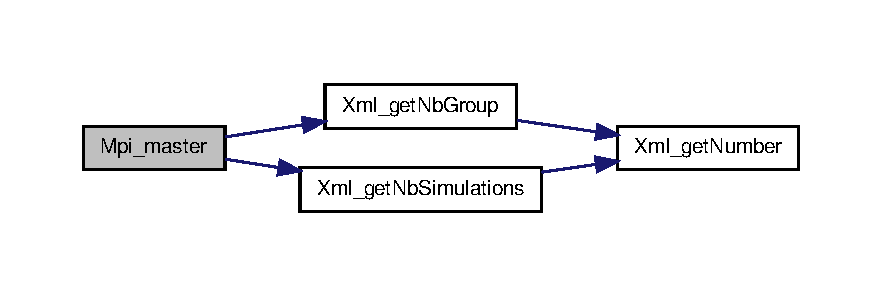
\includegraphics[width=400pt]{mpi__load_8h_a49f24c98f9724a9d2d64bf3b41d7c101_cgraph}
\end{center}
\end{figure}


\hypertarget{mpi__load_8h_ab4d2e0de3a14f863a405bddfa625b8bd}{
\index{mpi\_\-load.h@{mpi\_\-load.h}!Mpi\_\-sizeResultTab@{Mpi\_\-sizeResultTab}}
\index{Mpi\_\-sizeResultTab@{Mpi\_\-sizeResultTab}!mpi_load.h@{mpi\_\-load.h}}
\subsubsection[{Mpi\_\-sizeResultTab}]{\setlength{\rightskip}{0pt plus 5cm}int Mpi\_\-sizeResultTab (
\begin{DoxyParamCaption}
\item[{{\bf pListParameters}}]{allone, }
\item[{int}]{activity, }
\item[{int}]{group, }
\item[{int}]{nb\_\-species}
\end{DoxyParamCaption}
)}}
\label{mpi__load_8h_ab4d2e0de3a14f863a405bddfa625b8bd}


Determine the size of the result tab. 

\begin{DoxyAuthor}{Author}
Amine Ghozlane 
\end{DoxyAuthor}

\begin{DoxyParams}{Parameters}
{\em allone} & Global parameters : struct \hyperlink{structListParameters}{ListParameters} \\
\hline
{\em activity} & Chosen activity \\
\hline
{\em group} & Group flag \\
\hline
{\em nb\_\-species} & Number of interest species \\
\hline
\end{DoxyParams}
\begin{DoxyReturn}{Returns}
Size of Result tab 
\end{DoxyReturn}


Definition at line 334 of file mpi\_\-load.c.



References ListParameters::conf, ListParameters::model, ListParameters::nb\_\-parameters, and Xml\_\-getNbTriesMod().



Referenced by Mpi\_\-slave(), and Mpi\_\-writer().



Here is the call graph for this function:\nopagebreak
\begin{figure}[H]
\begin{center}
\leavevmode
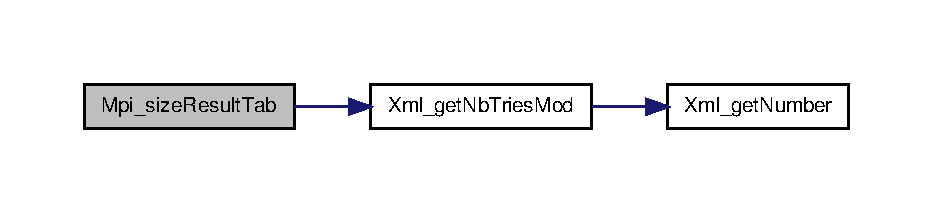
\includegraphics[width=400pt]{mpi__load_8h_ab4d2e0de3a14f863a405bddfa625b8bd_cgraph}
\end{center}
\end{figure}


\hypertarget{mpi__load_8h_a73a3042b31e240b5785eed805f963212}{
\index{mpi\_\-load.h@{mpi\_\-load.h}!Mpi\_\-slave@{Mpi\_\-slave}}
\index{Mpi\_\-slave@{Mpi\_\-slave}!mpi_load.h@{mpi\_\-load.h}}
\subsubsection[{Mpi\_\-slave}]{\setlength{\rightskip}{0pt plus 5cm}void Mpi\_\-slave (
\begin{DoxyParamCaption}
\item[{{\bf pListParameters}}]{allone, }
\item[{char $\ast$$\ast$}]{files\_\-path, }
\item[{int}]{activity, }
\item[{int}]{group, }
\item[{int}]{debug}
\end{DoxyParamCaption}
)}}
\label{mpi__load_8h_a73a3042b31e240b5785eed805f963212}
\begin{DoxyAuthor}{Author}
Amine Ghozlane 
\end{DoxyAuthor}

\begin{DoxyParams}{Parameters}
{\em allone} & Global parameters : struct \hyperlink{structListParameters}{ListParameters} \\
\hline
{\em files\_\-path} & List of paths \\
\hline
{\em activity} & Activity chosen \\
\hline
{\em group} & Group flag \\
\hline
{\em debug} & Debug flag \\
\hline
\end{DoxyParams}


Definition at line 440 of file mpi\_\-load.c.



References ListParameters::conf, Min\_\-compute\_\-minimization(), Mod\_\-compute\_\-modeling(), Mpi\_\-allocResultTab(), Mpi\_\-sizeResultTab(), ListParameters::nb\_\-parameters, Recuit\_\-compute\_\-recuit(), Sd\_\-compute\_\-standard\_\-deviation(), Xml\_\-getBoltzmann(), Xml\_\-getMuT(), Xml\_\-getNbIters(), Xml\_\-getNbSpecies(), Xml\_\-getNbTriesSa(), Xml\_\-getStepSize(), Xml\_\-getTinitial(), and Xml\_\-getTmin().



Referenced by compute\_\-mpi().



Here is the call graph for this function:\nopagebreak
\begin{figure}[H]
\begin{center}
\leavevmode
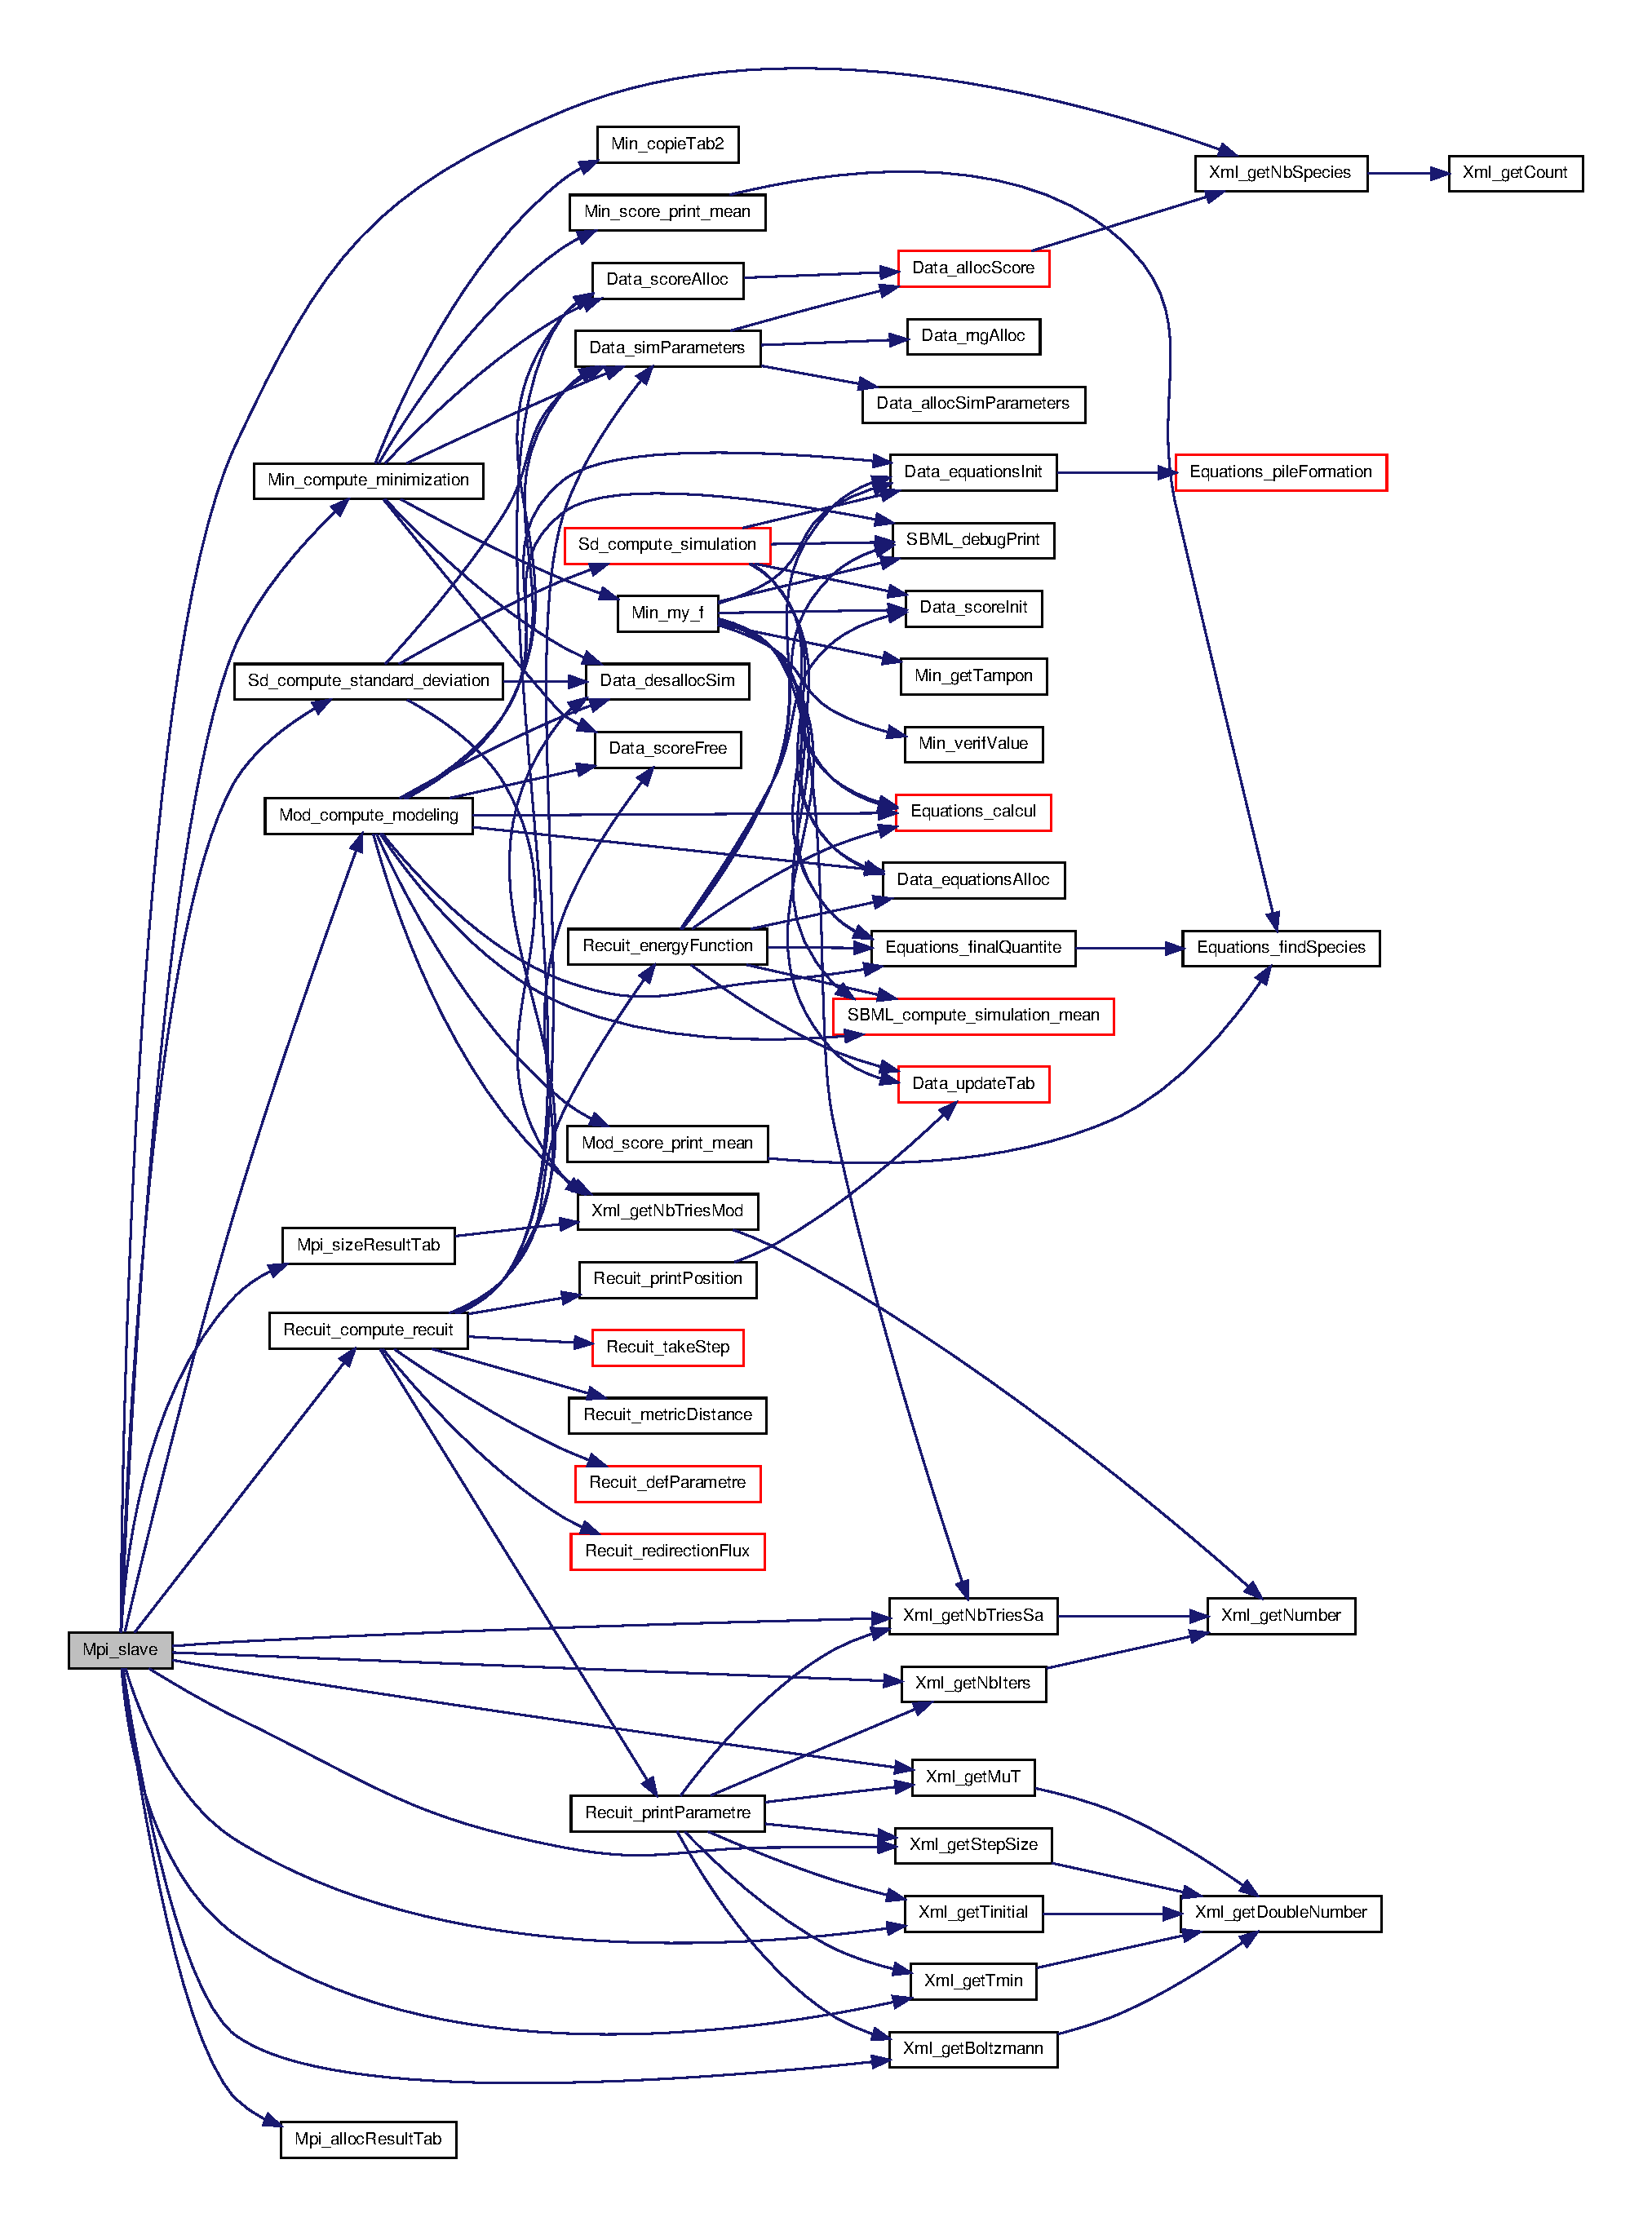
\includegraphics[width=400pt]{mpi__load_8h_a73a3042b31e240b5785eed805f963212_cgraph}
\end{center}
\end{figure}


\hypertarget{mpi__load_8h_a4cf3597a859457305000e2168f205993}{
\index{mpi\_\-load.h@{mpi\_\-load.h}!Mpi\_\-writer@{Mpi\_\-writer}}
\index{Mpi\_\-writer@{Mpi\_\-writer}!mpi_load.h@{mpi\_\-load.h}}
\subsubsection[{Mpi\_\-writer}]{\setlength{\rightskip}{0pt plus 5cm}void Mpi\_\-writer (
\begin{DoxyParamCaption}
\item[{{\bf pListParameters}}]{allone, }
\item[{char $\ast$$\ast$}]{files\_\-path, }
\item[{int}]{activity, }
\item[{int}]{group, }
\item[{int}]{myid}
\end{DoxyParamCaption}
)}}
\label{mpi__load_8h_a4cf3597a859457305000e2168f205993}


Master process. 

\begin{DoxyAuthor}{Author}
Amine Ghozlane 
\end{DoxyAuthor}

\begin{DoxyParams}{Parameters}
{\em allone} & Global parameters : struct \hyperlink{structListParameters}{ListParameters} \\
\hline
{\em files\_\-path} & List of paths \\
\hline
{\em activity} & Chosen activity \\
\hline
{\em group} & Group flag \\
\hline
{\em myid} & Id of the thread \\
\hline
\end{DoxyParams}


Definition at line 273 of file mpi\_\-load.c.



References ListParameters::conf, ListParameters::model, Mpi\_\-allocResultTab(), Mpi\_\-sizeResultTab(), Mpi\_\-writeSdFile(), Mpi\_\-writeSimFile(), and Xml\_\-getNbSpecies().



Referenced by compute\_\-mpi().



Here is the call graph for this function:\nopagebreak
\begin{figure}[H]
\begin{center}
\leavevmode
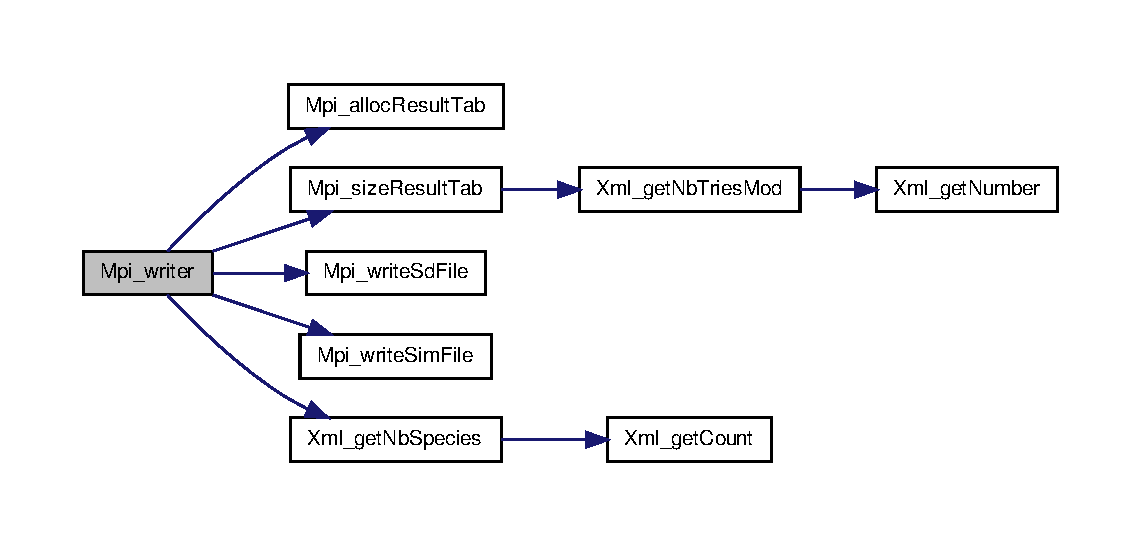
\includegraphics[width=400pt]{mpi__load_8h_a4cf3597a859457305000e2168f205993_cgraph}
\end{center}
\end{figure}


\hypertarget{mpi__load_8h_a3f0c05e595da1760ed46a5f5f978a704}{
\index{mpi\_\-load.h@{mpi\_\-load.h}!Mpi\_\-writeSdFile@{Mpi\_\-writeSdFile}}
\index{Mpi\_\-writeSdFile@{Mpi\_\-writeSdFile}!mpi_load.h@{mpi\_\-load.h}}
\subsubsection[{Mpi\_\-writeSdFile}]{\setlength{\rightskip}{0pt plus 5cm}void Mpi\_\-writeSdFile (
\begin{DoxyParamCaption}
\item[{FILE $\ast$}]{out, }
\item[{double $\ast$}]{result\_\-tab, }
\item[{int}]{tailleTab}
\end{DoxyParamCaption}
)}}
\label{mpi__load_8h_a3f0c05e595da1760ed46a5f5f978a704}


Determine the size of the result tab. 

\begin{DoxyAuthor}{Author}
Amine Ghozlane 
\end{DoxyAuthor}

\begin{DoxyParams}{Parameters}
{\em out} & Result file \\
\hline
{\em result\_\-tab} & Result table \\
\hline
{\em tailleTab} & Size of result table \\
\hline
\end{DoxyParams}


Definition at line 421 of file mpi\_\-load.c.



Referenced by Mpi\_\-writer().

\hypertarget{mpi__load_8h_aa753112f6c21ff66c1c63f511ccbb325}{
\index{mpi\_\-load.h@{mpi\_\-load.h}!Mpi\_\-writeSimFile@{Mpi\_\-writeSimFile}}
\index{Mpi\_\-writeSimFile@{Mpi\_\-writeSimFile}!mpi_load.h@{mpi\_\-load.h}}
\subsubsection[{Mpi\_\-writeSimFile}]{\setlength{\rightskip}{0pt plus 5cm}void Mpi\_\-writeSimFile (
\begin{DoxyParamCaption}
\item[{{\bf pListParameters}}]{allone, }
\item[{FILE $\ast$}]{out, }
\item[{FILE $\ast$}]{logOut, }
\item[{double $\ast$}]{result\_\-tab, }
\item[{int}]{group, }
\item[{int}]{tailleSpecies, }
\item[{int}]{nb\_\-species}
\end{DoxyParamCaption}
)}}
\label{mpi__load_8h_aa753112f6c21ff66c1c63f511ccbb325}


Determine the size of the result tab. 

\begin{DoxyAuthor}{Author}
Amine Ghozlane 
\end{DoxyAuthor}

\begin{DoxyParams}{Parameters}
{\em allone} & Global parameters : struct \hyperlink{structListParameters}{ListParameters} \\
\hline
{\em out} & Result file \\
\hline
{\em logOut} & Log file \\
\hline
{\em result\_\-tab} & Result table \\
\hline
{\em group} & Group flag \\
\hline
{\em tailleSpecies} & Number of species \\
\hline
{\em nb\_\-species} & Number of interest species \\
\hline
\end{DoxyParams}


Definition at line 375 of file mpi\_\-load.c.



References ListParameters::nb\_\-parameters.



Referenced by Mpi\_\-writer().


\hypertarget{simulation_8h}{
\section{metaboflux/include/simulation.h File Reference}
\label{simulation_8h}\index{metaboflux/include/simulation.h@{metaboflux/include/simulation.h}}
}


Simulate a petri net.  


This graph shows which files directly or indirectly include this file:\nopagebreak
\begin{figure}[H]
\begin{center}
\leavevmode
\includegraphics[width=400pt]{simulation_8h__dep__incl}
\end{center}
\end{figure}
\subsection*{Data Structures}
\begin{DoxyCompactItemize}
\item 
struct \hyperlink{structTestReaction}{TestReaction}
\begin{DoxyCompactList}\small\item\em Structure used to test reactions. \end{DoxyCompactList}\item 
struct \hyperlink{structScore}{Score}
\begin{DoxyCompactList}\small\item\em Structure containing all information from simulations. \end{DoxyCompactList}\end{DoxyCompactItemize}
\subsection*{Functions}
\begin{DoxyCompactItemize}
\item 
void \hyperlink{simulation_8h_a611031d9c60ad182fade6ae74e6b7e7e}{SBML\_\-initEspeceAmounts} (Model\_\-t $\ast$, \hyperlink{structEspeces}{pEspeces}, int)
\begin{DoxyCompactList}\small\item\em Alloc memory and initialize the struct \hyperlink{structEspeces}{Especes}. \end{DoxyCompactList}\item 
int \hyperlink{simulation_8h_acc2b5d50969ffb4eac4e86227f583b39}{SBML\_\-findReaction} (char $\ast$$\ast$, const char $\ast$, int)
\begin{DoxyCompactList}\small\item\em Determine if the reaction is study. \end{DoxyCompactList}\item 
double \hyperlink{simulation_8h_a97ee89b0e47e49cdcf5579255b8cd3a3}{SBML\_\-evalExpression} (const char $\ast$)
\begin{DoxyCompactList}\small\item\em Get the reaction ratio define in the sbml. \end{DoxyCompactList}\item 
void \hyperlink{simulation_8h_a4e69a993d7460adf46b17909e8991565}{SBML\_\-setReactions} (Model\_\-t $\ast$, \hyperlink{structEspeces}{pEspeces}, \hyperlink{structScore}{pScore}, double $\ast$, int, int)
\begin{DoxyCompactList}\small\item\em Alloc memory and initialize the struct \hyperlink{structEspeces}{Especes}. \end{DoxyCompactList}\item 
int \hyperlink{simulation_8h_a29d1d4fcf0dcc060769bf71e4e451b15}{SBML\_\-checkQuantite} (Model\_\-t $\ast$, Reaction\_\-t $\ast$, int, \hyperlink{structEspeces}{pEspeces})
\begin{DoxyCompactList}\small\item\em Determine the number of reaction for one molecule. \end{DoxyCompactList}\item 
Reaction\_\-t $\ast$ \hyperlink{simulation_8h_a8d9458c6636b5b95598434453ad6e3dd}{SBML\_\-reactChoice} (\hyperlink{structEspeces}{pEspeces}, const gsl\_\-rng $\ast$, int)
\begin{DoxyCompactList}\small\item\em Determine randomly the reaction to achieve for several nodes reactions. \end{DoxyCompactList}\item 
void \hyperlink{simulation_8h_a0421946146569268a97c95c27e57a65e}{SBML\_\-reaction} (Model\_\-t $\ast$, \hyperlink{structEspeces}{pEspeces}, Reaction\_\-t $\ast$, int)
\begin{DoxyCompactList}\small\item\em Simulation of a discrete transision. \end{DoxyCompactList}\item 
void \hyperlink{simulation_8h_abb6b027abfcddf0b783bdb3bc29e47d8}{SBML\_\-allocTest} (\hyperlink{structTestReaction}{pTestReaction}, int)
\begin{DoxyCompactList}\small\item\em Alloc memory and initialize the struct pTestReaction. \end{DoxyCompactList}\item 
void \hyperlink{simulation_8h_a9103674f503bec1df341d62554e1a9c2}{SBML\_\-freeTest} (\hyperlink{structTestReaction}{pTestReaction})
\begin{DoxyCompactList}\small\item\em Free memory of the struct \hyperlink{structTestReaction}{TestReaction}. \end{DoxyCompactList}\item 
int \hyperlink{simulation_8h_a5e7dd721fd4e49d51adaa2dd290879d4}{SBML\_\-EstimationReaction} (Model\_\-t $\ast$, \hyperlink{structTestReaction}{pTestReaction}, \hyperlink{structEspeces}{pEspeces}, int, int)
\begin{DoxyCompactList}\small\item\em Alloc memory and initialize the struct \hyperlink{structEspeces}{Especes}. \end{DoxyCompactList}\item 
int \hyperlink{simulation_8h_a79f018dd624b1b4a2ee36a2cb2939462}{SBML\_\-simulate} (Model\_\-t $\ast$, \hyperlink{structEspeces}{pEspeces}, const gsl\_\-rng $\ast$, \hyperlink{structTestReaction}{pTestReaction}, char $\ast$$\ast$, int, int, int)
\begin{DoxyCompactList}\small\item\em Simulate one step of petri net. \end{DoxyCompactList}\item 
void \hyperlink{simulation_8h_a0b14dd5a1a8cf318c2f7974bd9a8cc1c}{SBML\_\-score} (Model\_\-t $\ast$, \hyperlink{structEspeces}{pEspeces}, \hyperlink{structScore}{pScore}, double $\ast$, int, int)
\begin{DoxyCompactList}\small\item\em Alloc memory and initialize the struct \hyperlink{structEspeces}{Especes}. \end{DoxyCompactList}\item 
void \hyperlink{simulation_8h_a12fd385702f666987a4b569e84abed70}{SBML\_\-debugPrintHead} (FILE $\ast$, int, char $\ast$$\ast$)
\begin{DoxyCompactList}\small\item\em Print the head of the debug file. \end{DoxyCompactList}\item 
void \hyperlink{simulation_8h_a69e2b7c32f7b66e66d28030d00917fd7}{SBML\_\-debugPrint} (FILE $\ast$, int, int, double $\ast$, double)
\begin{DoxyCompactList}\small\item\em Print the debuf file. \end{DoxyCompactList}\item 
void \hyperlink{simulation_8h_a443eccd5296f1a2844c4d97e514a61c5}{SBML\_\-compute\_\-simulation} (\hyperlink{structScore}{pScore}, Model\_\-t $\ast$, double $\ast$, gsl\_\-rng $\ast$, char $\ast$$\ast$, int)
\begin{DoxyCompactList}\small\item\em Simulation of metabolic network. \end{DoxyCompactList}\item 
void \hyperlink{simulation_8h_a97ba6b434d34399d17103fbb366afd74}{SBML\_\-score\_\-add} (\hyperlink{structScore}{pScore}, \hyperlink{structScore}{pScore}, FILE $\ast$)
\begin{DoxyCompactList}\small\item\em Add scores. \end{DoxyCompactList}\item 
void \hyperlink{simulation_8h_a785b8432d885cc9e8ef50413c3643f6a}{SBML\_\-score\_\-mean} (\hyperlink{structScore}{pScore}, int)
\begin{DoxyCompactList}\small\item\em Mean quantities for score. \end{DoxyCompactList}\item 
void \hyperlink{simulation_8h_a16b0c1105bbcfc7ddc9a9e044d567ed5}{SBML\_\-compute\_\-simulation\_\-mean} (FILE $\ast$, \hyperlink{structScore}{pScore}, \hyperlink{structScore}{pScore}, Model\_\-t $\ast$, double $\ast$, gsl\_\-rng $\ast$, char $\ast$$\ast$, int, int)
\begin{DoxyCompactList}\small\item\em X time simulation of metabolic network. \end{DoxyCompactList}\end{DoxyCompactItemize}


\subsection{Detailed Description}
Simulate a petri net. This file is part of MetaBoFlux (\href{http://www.cbib.u-bordeaux2.fr/metaboflux/}{\tt http://www.cbib.u-\/bordeaux2.fr/metaboflux/}) Copyright (C) 2010 Amine Ghozlane from LaBRI and University of Bordeaux 1

MetaBoFlux is free software: you can redistribute it and/or modify it under the terms of the GNU Lesser General Public License as published by the Free Software Foundation, either version 3 of the License, or (at your option) any later version.

MetaBoFlux is distributed in the hope that it will be useful, but WITHOUT ANY WARRANTY; without even the implied warranty of MERCHANTABILITY or FITNESS FOR A PARTICULAR PURPOSE. See the GNU General Public License for more details.

You should have received a copy of the GNU Lesser General Public License along with this program. If not, see $<$\href{http://www.gnu.org/licenses/}{\tt http://www.gnu.org/licenses/}$>$.

\begin{DoxyAuthor}{Author}
\{Amine Ghozlane\} 
\end{DoxyAuthor}
\begin{DoxyVersion}{Version}
2.0 
\end{DoxyVersion}
\begin{DoxyDate}{Date}
27 octobre 2009 
\end{DoxyDate}


Definition in file \hyperlink{simulation_8h_source}{simulation.h}.



\subsection{Function Documentation}
\hypertarget{simulation_8h_abb6b027abfcddf0b783bdb3bc29e47d8}{
\index{simulation.h@{simulation.h}!SBML\_\-allocTest@{SBML\_\-allocTest}}
\index{SBML\_\-allocTest@{SBML\_\-allocTest}!simulation.h@{simulation.h}}
\subsubsection[{SBML\_\-allocTest}]{\setlength{\rightskip}{0pt plus 5cm}void SBML\_\-allocTest (
\begin{DoxyParamCaption}
\item[{{\bf pTestReaction}}]{T, }
\item[{int}]{nbReactions}
\end{DoxyParamCaption}
)}}
\label{simulation_8h_abb6b027abfcddf0b783bdb3bc29e47d8}


Alloc memory and initialize the struct pTestReaction. 

\begin{DoxyAuthor}{Author}
Amine Ghozlane 
\end{DoxyAuthor}

\begin{DoxyParams}{Parameters}
{\em T} & Empty struct \hyperlink{structTestReaction}{TestReaction} \\
\hline
{\em nbReactions} & Number of reactions \\
\hline
\end{DoxyParams}


Definition at line 279 of file simulation.c.



References TestReaction::minStepTab, and TestReaction::tabReactions.



Referenced by SBML\_\-simulate().

\hypertarget{simulation_8h_a29d1d4fcf0dcc060769bf71e4e451b15}{
\index{simulation.h@{simulation.h}!SBML\_\-checkQuantite@{SBML\_\-checkQuantite}}
\index{SBML\_\-checkQuantite@{SBML\_\-checkQuantite}!simulation.h@{simulation.h}}
\subsubsection[{SBML\_\-checkQuantite}]{\setlength{\rightskip}{0pt plus 5cm}int SBML\_\-checkQuantite (
\begin{DoxyParamCaption}
\item[{Model\_\-t $\ast$}]{mod, }
\item[{Reaction\_\-t $\ast$}]{react, }
\item[{int}]{nbEspeces, }
\item[{{\bf pEspeces}}]{molecules}
\end{DoxyParamCaption}
)}}
\label{simulation_8h_a29d1d4fcf0dcc060769bf71e4e451b15}


Determine the number of reaction for one molecule. 

\begin{DoxyAuthor}{Author}
Amine Ghozlane 
\end{DoxyAuthor}

\begin{DoxyParams}{Parameters}
{\em mod} & Model of the SBML file \\
\hline
{\em react} & \hyperlink{structReaction}{Reaction} id \\
\hline
{\em nbEspeces} & Number of molecules \\
\hline
{\em molecules} & Struct \hyperlink{structEspeces}{Especes} \\
\hline
\end{DoxyParams}
\begin{DoxyReturn}{Returns}
Number of reaction for one molecule 
\end{DoxyReturn}


Definition at line 158 of file simulation.c.



References Especes\_\-find(), and Especes\_\-getQuantite().



Referenced by SBML\_\-EstimationReaction(), and SBML\_\-simulate().



Here is the call graph for this function:\nopagebreak
\begin{figure}[H]
\begin{center}
\leavevmode
\includegraphics[width=338pt]{simulation_8h_a29d1d4fcf0dcc060769bf71e4e451b15_cgraph}
\end{center}
\end{figure}


\hypertarget{simulation_8h_a443eccd5296f1a2844c4d97e514a61c5}{
\index{simulation.h@{simulation.h}!SBML\_\-compute\_\-simulation@{SBML\_\-compute\_\-simulation}}
\index{SBML\_\-compute\_\-simulation@{SBML\_\-compute\_\-simulation}!simulation.h@{simulation.h}}
\subsubsection[{SBML\_\-compute\_\-simulation}]{\setlength{\rightskip}{0pt plus 5cm}void SBML\_\-compute\_\-simulation (
\begin{DoxyParamCaption}
\item[{{\bf pScore}}]{result, }
\item[{Model\_\-t $\ast$}]{mod, }
\item[{double $\ast$}]{reactions\_\-ratio, }
\item[{gsl\_\-rng $\ast$}]{r, }
\item[{char $\ast$$\ast$}]{banned, }
\item[{int}]{nbBanned}
\end{DoxyParamCaption}
)}}
\label{simulation_8h_a443eccd5296f1a2844c4d97e514a61c5}


Simulation of metabolic network. 

\begin{DoxyAuthor}{Author}
Amine Ghozlane 
\end{DoxyAuthor}

\begin{DoxyParams}{Parameters}
{\em result} & Struct \hyperlink{structScore}{Score} \\
\hline
{\em mod} & Model of the SBML file \\
\hline
{\em reactions\_\-ratio} & List of computed reaction ratio \\
\hline
{\em r} & Random number generator \\
\hline
{\em banned} & List of banned compound \\
\hline
{\em nbBanned} & Number of banned compound \\
\hline
\end{DoxyParams}


Definition at line 515 of file simulation.c.



References Especes\_\-alloc(), Especes\_\-free(), SBML\_\-initEspeceAmounts(), SBML\_\-score(), SBML\_\-setReactions(), SBML\_\-simulate(), Score::tailleReactions, and Score::tailleSpecies.



Referenced by Sd\_\-compute\_\-simulation().



Here is the call graph for this function:\nopagebreak
\begin{figure}[H]
\begin{center}
\leavevmode
\includegraphics[width=400pt]{simulation_8h_a443eccd5296f1a2844c4d97e514a61c5_cgraph}
\end{center}
\end{figure}


\hypertarget{simulation_8h_a16b0c1105bbcfc7ddc9a9e044d567ed5}{
\index{simulation.h@{simulation.h}!SBML\_\-compute\_\-simulation\_\-mean@{SBML\_\-compute\_\-simulation\_\-mean}}
\index{SBML\_\-compute\_\-simulation\_\-mean@{SBML\_\-compute\_\-simulation\_\-mean}!simulation.h@{simulation.h}}
\subsubsection[{SBML\_\-compute\_\-simulation\_\-mean}]{\setlength{\rightskip}{0pt plus 5cm}void SBML\_\-compute\_\-simulation\_\-mean (
\begin{DoxyParamCaption}
\item[{FILE $\ast$}]{debugFile, }
\item[{{\bf pScore}}]{result, }
\item[{{\bf pScore}}]{result\_\-temp, }
\item[{Model\_\-t $\ast$}]{mod, }
\item[{double $\ast$}]{reactions\_\-ratio, }
\item[{gsl\_\-rng $\ast$}]{r, }
\item[{char $\ast$$\ast$}]{banned, }
\item[{int}]{nbBanned, }
\item[{int}]{nb\_\-simulation}
\end{DoxyParamCaption}
)}}
\label{simulation_8h_a16b0c1105bbcfc7ddc9a9e044d567ed5}


X time simulation of metabolic network. 

\begin{DoxyAuthor}{Author}
Amine Ghozlane 
\end{DoxyAuthor}

\begin{DoxyParams}{Parameters}
{\em debugFile} & File use for debug \\
\hline
{\em result} & Struct \hyperlink{structScore}{Score} used for all the simulation \\
\hline
{\em result\_\-temp} & Struct \hyperlink{structScore}{Score} used at each simulation step \\
\hline
{\em mod} & Model of the SBML file \\
\hline
{\em reactions\_\-ratio} & List of computed reaction ratio \\
\hline
{\em r} & Random number generator \\
\hline
{\em banned} & List of banned compound \\
\hline
{\em nbBanned} & Number of banned compound \\
\hline
{\em nb\_\-simulation} & Number of simulation step \\
\hline
\end{DoxyParams}


Definition at line 614 of file simulation.c.



References Especes\_\-alloc(), Especes\_\-free(), SBML\_\-initEspeceAmounts(), SBML\_\-score(), SBML\_\-score\_\-add(), SBML\_\-score\_\-mean(), SBML\_\-setReactions(), and SBML\_\-simulate().



Referenced by Min\_\-my\_\-f(), Mod\_\-compute\_\-modeling(), and Recuit\_\-energyFunction().



Here is the call graph for this function:\nopagebreak
\begin{figure}[H]
\begin{center}
\leavevmode
\includegraphics[width=400pt]{simulation_8h_a16b0c1105bbcfc7ddc9a9e044d567ed5_cgraph}
\end{center}
\end{figure}


\hypertarget{simulation_8h_a69e2b7c32f7b66e66d28030d00917fd7}{
\index{simulation.h@{simulation.h}!SBML\_\-debugPrint@{SBML\_\-debugPrint}}
\index{SBML\_\-debugPrint@{SBML\_\-debugPrint}!simulation.h@{simulation.h}}
\subsubsection[{SBML\_\-debugPrint}]{\setlength{\rightskip}{0pt plus 5cm}void SBML\_\-debugPrint (
\begin{DoxyParamCaption}
\item[{FILE $\ast$}]{debugFile, }
\item[{int}]{tailleSpecies, }
\item[{int}]{taille, }
\item[{double $\ast$}]{quantite, }
\item[{double}]{result}
\end{DoxyParamCaption}
)}}
\label{simulation_8h_a69e2b7c32f7b66e66d28030d00917fd7}


Print the debuf file. 

\begin{DoxyAuthor}{Author}
Amine Ghozlane 
\end{DoxyAuthor}

\begin{DoxyParams}{Parameters}
{\em debugFile} & File use for debug \\
\hline
{\em tailleSpecies} & Number of molecules \\
\hline
{\em taille} & Number of molecules/reactions \\
\hline
{\em quantite} & Quantity of molecules/reactions \\
\hline
{\em result} & Energy value \\
\hline
\end{DoxyParams}


Definition at line 486 of file simulation.c.



Referenced by Min\_\-my\_\-f(), Mod\_\-compute\_\-modeling(), Recuit\_\-energyFunction(), SBML\_\-score\_\-add(), and Sd\_\-compute\_\-simulation().

\hypertarget{simulation_8h_a12fd385702f666987a4b569e84abed70}{
\index{simulation.h@{simulation.h}!SBML\_\-debugPrintHead@{SBML\_\-debugPrintHead}}
\index{SBML\_\-debugPrintHead@{SBML\_\-debugPrintHead}!simulation.h@{simulation.h}}
\subsubsection[{SBML\_\-debugPrintHead}]{\setlength{\rightskip}{0pt plus 5cm}void SBML\_\-debugPrintHead (
\begin{DoxyParamCaption}
\item[{FILE $\ast$}]{debugFile, }
\item[{int}]{taille, }
\item[{char $\ast$$\ast$}]{name}
\end{DoxyParamCaption}
)}}
\label{simulation_8h_a12fd385702f666987a4b569e84abed70}


Print the head of the debug file. 

\begin{DoxyAuthor}{Author}
Amine Ghozlane 
\end{DoxyAuthor}

\begin{DoxyParams}{Parameters}
{\em debugFile} & File use for debug \\
\hline
{\em taille} & Number of molecules/reactions \\
\hline
{\em name} & List of molecules/reactions \\
\hline
\end{DoxyParams}


Definition at line 465 of file simulation.c.



Referenced by SBML\_\-score\_\-add(), and Sd\_\-compute\_\-simulation().

\hypertarget{simulation_8h_a5e7dd721fd4e49d51adaa2dd290879d4}{
\index{simulation.h@{simulation.h}!SBML\_\-EstimationReaction@{SBML\_\-EstimationReaction}}
\index{SBML\_\-EstimationReaction@{SBML\_\-EstimationReaction}!simulation.h@{simulation.h}}
\subsubsection[{SBML\_\-EstimationReaction}]{\setlength{\rightskip}{0pt plus 5cm}int SBML\_\-EstimationReaction (
\begin{DoxyParamCaption}
\item[{Model\_\-t $\ast$}]{mod, }
\item[{{\bf pTestReaction}}]{T, }
\item[{{\bf pEspeces}}]{molecules, }
\item[{int}]{ref, }
\item[{int}]{nbEspeces}
\end{DoxyParamCaption}
)}}
\label{simulation_8h_a5e7dd721fd4e49d51adaa2dd290879d4}


Alloc memory and initialize the struct \hyperlink{structEspeces}{Especes}. 

\begin{DoxyAuthor}{Author}
Amine Ghozlane 
\end{DoxyAuthor}

\begin{DoxyParams}{Parameters}
{\em mod} & Model of the SBML file \\
\hline
{\em T} & Struct \hyperlink{structTestReaction}{TestReaction} gives data on reaction \\
\hline
{\em molecules} & Struct \hyperlink{structEspeces}{Especes} \\
\hline
{\em ref} & Number reference of one molecule \\
\hline
{\em nbEspeces} & Number of molecules \\
\hline
\end{DoxyParams}
\begin{DoxyReturn}{Returns}
Estimated number of feasible step by reaction 
\end{DoxyReturn}


Definition at line 322 of file simulation.c.



References Reaction::link, TestReaction::minStepTab, SBML\_\-checkQuantite(), Reaction::suivant, Especes::system, and TestReaction::tabReactions.



Referenced by SBML\_\-simulate().



Here is the call graph for this function:\nopagebreak
\begin{figure}[H]
\begin{center}
\leavevmode
\includegraphics[width=400pt]{simulation_8h_a5e7dd721fd4e49d51adaa2dd290879d4_cgraph}
\end{center}
\end{figure}


\hypertarget{simulation_8h_a97ee89b0e47e49cdcf5579255b8cd3a3}{
\index{simulation.h@{simulation.h}!SBML\_\-evalExpression@{SBML\_\-evalExpression}}
\index{SBML\_\-evalExpression@{SBML\_\-evalExpression}!simulation.h@{simulation.h}}
\subsubsection[{SBML\_\-evalExpression}]{\setlength{\rightskip}{0pt plus 5cm}double SBML\_\-evalExpression (
\begin{DoxyParamCaption}
\item[{const char $\ast$}]{formule}
\end{DoxyParamCaption}
)}}
\label{simulation_8h_a97ee89b0e47e49cdcf5579255b8cd3a3}


Get the reaction ratio define in the sbml. 

\begin{DoxyAuthor}{Author}
Amine Ghozlane 
\end{DoxyAuthor}

\begin{DoxyParams}{Parameters}
{\em formule} & Formule SBML \\
\hline
\end{DoxyParams}
\begin{DoxyReturn}{Returns}
Return double value of the constraint 
\end{DoxyReturn}


Definition at line 88 of file simulation.c.



Referenced by SBML\_\-score(), and SBML\_\-setReactions().

\hypertarget{simulation_8h_acc2b5d50969ffb4eac4e86227f583b39}{
\index{simulation.h@{simulation.h}!SBML\_\-findReaction@{SBML\_\-findReaction}}
\index{SBML\_\-findReaction@{SBML\_\-findReaction}!simulation.h@{simulation.h}}
\subsubsection[{SBML\_\-findReaction}]{\setlength{\rightskip}{0pt plus 5cm}int SBML\_\-findReaction (
\begin{DoxyParamCaption}
\item[{char $\ast$$\ast$}]{reaction, }
\item[{const char $\ast$}]{react, }
\item[{int}]{nb\_\-reaction}
\end{DoxyParamCaption}
)}}
\label{simulation_8h_acc2b5d50969ffb4eac4e86227f583b39}


Determine if the reaction is study. 

\begin{DoxyAuthor}{Author}
Amine Ghozlane 
\end{DoxyAuthor}

\begin{DoxyParams}{Parameters}
{\em reaction} & List of reactions \\
\hline
{\em react} & \hyperlink{structReaction}{Reaction} of interest \\
\hline
{\em nb\_\-reaction} & Number of reactions \\
\hline
\end{DoxyParams}
\begin{DoxyReturn}{Returns}
Number of the molecules if it's study 
\end{DoxyReturn}


Definition at line 69 of file simulation.c.



Referenced by SBML\_\-score(), and SBML\_\-setReactions().

\hypertarget{simulation_8h_a9103674f503bec1df341d62554e1a9c2}{
\index{simulation.h@{simulation.h}!SBML\_\-freeTest@{SBML\_\-freeTest}}
\index{SBML\_\-freeTest@{SBML\_\-freeTest}!simulation.h@{simulation.h}}
\subsubsection[{SBML\_\-freeTest}]{\setlength{\rightskip}{0pt plus 5cm}void SBML\_\-freeTest (
\begin{DoxyParamCaption}
\item[{{\bf pTestReaction}}]{T}
\end{DoxyParamCaption}
)}}
\label{simulation_8h_a9103674f503bec1df341d62554e1a9c2}


Free memory of the struct \hyperlink{structTestReaction}{TestReaction}. 

\begin{DoxyAuthor}{Author}
Amine Ghozlane 
\end{DoxyAuthor}

\begin{DoxyParams}{Parameters}
{\em T} & Struct \hyperlink{structTestReaction}{TestReaction} gives data on reaction \\
\hline
\end{DoxyParams}


Definition at line 304 of file simulation.c.



References TestReaction::minStepTab, and TestReaction::tabReactions.



Referenced by SBML\_\-simulate().

\hypertarget{simulation_8h_a611031d9c60ad182fade6ae74e6b7e7e}{
\index{simulation.h@{simulation.h}!SBML\_\-initEspeceAmounts@{SBML\_\-initEspeceAmounts}}
\index{SBML\_\-initEspeceAmounts@{SBML\_\-initEspeceAmounts}!simulation.h@{simulation.h}}
\subsubsection[{SBML\_\-initEspeceAmounts}]{\setlength{\rightskip}{0pt plus 5cm}void SBML\_\-initEspeceAmounts (
\begin{DoxyParamCaption}
\item[{Model\_\-t $\ast$}]{mod, }
\item[{{\bf pEspeces}}]{molecules, }
\item[{int}]{nbEspeces}
\end{DoxyParamCaption}
)}}
\label{simulation_8h_a611031d9c60ad182fade6ae74e6b7e7e}


Alloc memory and initialize the struct \hyperlink{structEspeces}{Especes}. 

\begin{DoxyAuthor}{Author}
Amine Ghozlane 
\end{DoxyAuthor}

\begin{DoxyParams}{Parameters}
{\em mod} & Model of the SBML file \\
\hline
{\em molecules} & Struct \hyperlink{structEspeces}{Especes} \\
\hline
{\em nbEspeces} & Number of molecules \\
\hline
\end{DoxyParams}


Definition at line 46 of file simulation.c.



References Especes\_\-save().



Referenced by SBML\_\-compute\_\-simulation(), and SBML\_\-compute\_\-simulation\_\-mean().



Here is the call graph for this function:\nopagebreak
\begin{figure}[H]
\begin{center}
\leavevmode
\includegraphics[width=332pt]{simulation_8h_a611031d9c60ad182fade6ae74e6b7e7e_cgraph}
\end{center}
\end{figure}


\hypertarget{simulation_8h_a8d9458c6636b5b95598434453ad6e3dd}{
\index{simulation.h@{simulation.h}!SBML\_\-reactChoice@{SBML\_\-reactChoice}}
\index{SBML\_\-reactChoice@{SBML\_\-reactChoice}!simulation.h@{simulation.h}}
\subsubsection[{SBML\_\-reactChoice}]{\setlength{\rightskip}{0pt plus 5cm}Reaction\_\-t$\ast$ SBML\_\-reactChoice (
\begin{DoxyParamCaption}
\item[{{\bf pEspeces}}]{molecules, }
\item[{const gsl\_\-rng $\ast$}]{r, }
\item[{int}]{ref}
\end{DoxyParamCaption}
)}}
\label{simulation_8h_a8d9458c6636b5b95598434453ad6e3dd}


Determine randomly the reaction to achieve for several nodes reactions. 

\begin{DoxyAuthor}{Author}
Amine Ghozlane 
\end{DoxyAuthor}

\begin{DoxyParams}{Parameters}
{\em molecules} & Struct \hyperlink{structEspeces}{Especes} \\
\hline
{\em r} & Random number generator \\
\hline
{\em ref} & Number reference of one molecule \\
\hline
\end{DoxyParams}
\begin{DoxyReturn}{Returns}
Id of the selected reaction 
\end{DoxyReturn}


Definition at line 206 of file simulation.c.



References Reaction::link, Reaction::suivant, and Especes::system.



Referenced by SBML\_\-simulate().

\hypertarget{simulation_8h_a0421946146569268a97c95c27e57a65e}{
\index{simulation.h@{simulation.h}!SBML\_\-reaction@{SBML\_\-reaction}}
\index{SBML\_\-reaction@{SBML\_\-reaction}!simulation.h@{simulation.h}}
\subsubsection[{SBML\_\-reaction}]{\setlength{\rightskip}{0pt plus 5cm}void SBML\_\-reaction (
\begin{DoxyParamCaption}
\item[{Model\_\-t $\ast$}]{mod, }
\item[{{\bf pEspeces}}]{molecules, }
\item[{Reaction\_\-t $\ast$}]{react, }
\item[{int}]{nbEspeces}
\end{DoxyParamCaption}
)}}
\label{simulation_8h_a0421946146569268a97c95c27e57a65e}


Simulation of a discrete transision. 

\begin{DoxyAuthor}{Author}
Amine Ghozlane 
\end{DoxyAuthor}

\begin{DoxyParams}{Parameters}
{\em mod} & Model of the SBML file \\
\hline
{\em molecules} & Struct \hyperlink{structEspeces}{Especes} \\
\hline
{\em react} & \hyperlink{structReaction}{Reaction} id \\
\hline
{\em nbEspeces} & Number of molecules \\
\hline
\end{DoxyParams}


Definition at line 244 of file simulation.c.



References Especes\_\-find(), Especes\_\-getQuantite(), and Especes\_\-setQuantite().



Referenced by SBML\_\-simulate().



Here is the call graph for this function:\nopagebreak
\begin{figure}[H]
\begin{center}
\leavevmode
\includegraphics[width=310pt]{simulation_8h_a0421946146569268a97c95c27e57a65e_cgraph}
\end{center}
\end{figure}


\hypertarget{simulation_8h_a0b14dd5a1a8cf318c2f7974bd9a8cc1c}{
\index{simulation.h@{simulation.h}!SBML\_\-score@{SBML\_\-score}}
\index{SBML\_\-score@{SBML\_\-score}!simulation.h@{simulation.h}}
\subsubsection[{SBML\_\-score}]{\setlength{\rightskip}{0pt plus 5cm}void SBML\_\-score (
\begin{DoxyParamCaption}
\item[{Model\_\-t $\ast$}]{mod, }
\item[{{\bf pEspeces}}]{molecules, }
\item[{{\bf pScore}}]{result, }
\item[{double $\ast$}]{reactions\_\-ratio, }
\item[{int}]{nbReactions, }
\item[{int}]{nbEspeces}
\end{DoxyParamCaption}
)}}
\label{simulation_8h_a0b14dd5a1a8cf318c2f7974bd9a8cc1c}


Alloc memory and initialize the struct \hyperlink{structEspeces}{Especes}. 

\begin{DoxyAuthor}{Author}
Amine Ghozlane 
\end{DoxyAuthor}

\begin{DoxyParams}{Parameters}
{\em mod} & Model of the SBML file \\
\hline
{\em molecules} & Struct \hyperlink{structEspeces}{Especes} \\
\hline
{\em result} & Struct \hyperlink{structScore}{Score} \\
\hline
{\em reactions\_\-ratio} & List of computed reaction ratio \\
\hline
{\em nbReactions} & Number of reactions \\
\hline
{\em nbEspeces} & Number of molecules \\
\hline
\end{DoxyParams}


Definition at line 420 of file simulation.c.



References Especes\_\-scoreSpecies(), Score::name, Score::nb\_\-reaction, Score::quantite, Score::reaction, SBML\_\-evalExpression(), and SBML\_\-findReaction().



Referenced by SBML\_\-compute\_\-simulation(), and SBML\_\-compute\_\-simulation\_\-mean().



Here is the call graph for this function:\nopagebreak
\begin{figure}[H]
\begin{center}
\leavevmode
\includegraphics[width=310pt]{simulation_8h_a0b14dd5a1a8cf318c2f7974bd9a8cc1c_cgraph}
\end{center}
\end{figure}


\hypertarget{simulation_8h_a97ba6b434d34399d17103fbb366afd74}{
\index{simulation.h@{simulation.h}!SBML\_\-score\_\-add@{SBML\_\-score\_\-add}}
\index{SBML\_\-score\_\-add@{SBML\_\-score\_\-add}!simulation.h@{simulation.h}}
\subsubsection[{SBML\_\-score\_\-add}]{\setlength{\rightskip}{0pt plus 5cm}void SBML\_\-score\_\-add (
\begin{DoxyParamCaption}
\item[{{\bf pScore}}]{result, }
\item[{{\bf pScore}}]{result\_\-temp, }
\item[{FILE $\ast$}]{debugFile}
\end{DoxyParamCaption}
)}}
\label{simulation_8h_a97ba6b434d34399d17103fbb366afd74}


Add scores. 

\begin{DoxyAuthor}{Author}
Amine Ghozlane 
\end{DoxyAuthor}

\begin{DoxyParams}{Parameters}
{\em result} & Struct \hyperlink{structScore}{Score} used for all the simulation \\
\hline
{\em result\_\-temp} & Struct \hyperlink{structScore}{Score} used at each simulation step \\
\hline
{\em debugFile} & File use for debug \\
\hline
\end{DoxyParams}


Definition at line 560 of file simulation.c.



References Score::name, Score::quantite, SBML\_\-debugPrint(), SBML\_\-debugPrintHead(), Score::taille, and Score::tailleSpecies.



Referenced by SBML\_\-compute\_\-simulation\_\-mean().



Here is the call graph for this function:\nopagebreak
\begin{figure}[H]
\begin{center}
\leavevmode
\includegraphics[width=330pt]{simulation_8h_a97ba6b434d34399d17103fbb366afd74_cgraph}
\end{center}
\end{figure}


\hypertarget{simulation_8h_a785b8432d885cc9e8ef50413c3643f6a}{
\index{simulation.h@{simulation.h}!SBML\_\-score\_\-mean@{SBML\_\-score\_\-mean}}
\index{SBML\_\-score\_\-mean@{SBML\_\-score\_\-mean}!simulation.h@{simulation.h}}
\subsubsection[{SBML\_\-score\_\-mean}]{\setlength{\rightskip}{0pt plus 5cm}void SBML\_\-score\_\-mean (
\begin{DoxyParamCaption}
\item[{{\bf pScore}}]{result, }
\item[{int}]{n}
\end{DoxyParamCaption}
)}}
\label{simulation_8h_a785b8432d885cc9e8ef50413c3643f6a}


Mean quantities for score. 

\begin{DoxyAuthor}{Author}
Amine Ghozlane 
\end{DoxyAuthor}

\begin{DoxyParams}{Parameters}
{\em result} & Struct \hyperlink{structScore}{Score} \\
\hline
{\em n} & Number of simulation step \\
\hline
\end{DoxyParams}


Definition at line 591 of file simulation.c.



References Score::quantite, and Score::taille.



Referenced by SBML\_\-compute\_\-simulation\_\-mean().

\hypertarget{simulation_8h_a4e69a993d7460adf46b17909e8991565}{
\index{simulation.h@{simulation.h}!SBML\_\-setReactions@{SBML\_\-setReactions}}
\index{SBML\_\-setReactions@{SBML\_\-setReactions}!simulation.h@{simulation.h}}
\subsubsection[{SBML\_\-setReactions}]{\setlength{\rightskip}{0pt plus 5cm}void SBML\_\-setReactions (
\begin{DoxyParamCaption}
\item[{Model\_\-t $\ast$}]{mod, }
\item[{{\bf pEspeces}}]{molecules, }
\item[{{\bf pScore}}]{result, }
\item[{double $\ast$}]{reactions\_\-ratio, }
\item[{int}]{nbReactions, }
\item[{int}]{nbEspeces}
\end{DoxyParamCaption}
)}}
\label{simulation_8h_a4e69a993d7460adf46b17909e8991565}


Alloc memory and initialize the struct \hyperlink{structEspeces}{Especes}. 

\begin{DoxyAuthor}{Author}
Amine Ghozlane 
\end{DoxyAuthor}

\begin{DoxyParams}{Parameters}
{\em mod} & Model of the SBML file \\
\hline
{\em molecules} & Struct \hyperlink{structEspeces}{Especes} \\
\hline
{\em result} & Struct \hyperlink{structScore}{Score} \\
\hline
{\em reactions\_\-ratio} & List of computed reaction ratio \\
\hline
{\em nbReactions} & Number of reaction \\
\hline
{\em nbEspeces} & Number of molecules \\
\hline
\end{DoxyParams}


Definition at line 105 of file simulation.c.



References Especes\_\-allocReactions(), Especes\_\-find(), Score::nb\_\-reaction, Score::reaction, SBML\_\-evalExpression(), and SBML\_\-findReaction().



Referenced by SBML\_\-compute\_\-simulation(), and SBML\_\-compute\_\-simulation\_\-mean().



Here is the call graph for this function:\nopagebreak
\begin{figure}[H]
\begin{center}
\leavevmode
\includegraphics[width=350pt]{simulation_8h_a4e69a993d7460adf46b17909e8991565_cgraph}
\end{center}
\end{figure}


\hypertarget{simulation_8h_a79f018dd624b1b4a2ee36a2cb2939462}{
\index{simulation.h@{simulation.h}!SBML\_\-simulate@{SBML\_\-simulate}}
\index{SBML\_\-simulate@{SBML\_\-simulate}!simulation.h@{simulation.h}}
\subsubsection[{SBML\_\-simulate}]{\setlength{\rightskip}{0pt plus 5cm}int SBML\_\-simulate (
\begin{DoxyParamCaption}
\item[{Model\_\-t $\ast$}]{mod, }
\item[{{\bf pEspeces}}]{molecules, }
\item[{const gsl\_\-rng $\ast$}]{r, }
\item[{{\bf pTestReaction}}]{T, }
\item[{char $\ast$$\ast$}]{banned, }
\item[{int}]{nbBanned, }
\item[{int}]{nbEspeces, }
\item[{int}]{ref}
\end{DoxyParamCaption}
)}}
\label{simulation_8h_a79f018dd624b1b4a2ee36a2cb2939462}


Simulate one step of petri net. 

\begin{DoxyAuthor}{Author}
Amine Ghozlane 
\end{DoxyAuthor}

\begin{DoxyParams}{Parameters}
{\em mod} & Model of the SBML file \\
\hline
{\em molecules} & Struct \hyperlink{structEspeces}{Especes} \\
\hline
{\em r} & Random number generator \\
\hline
{\em T} & Struct \hyperlink{structTestReaction}{TestReaction} gives data on reaction \\
\hline
{\em banned} & List of banned compound \\
\hline
{\em nbBanned} & Number of banned compound \\
\hline
{\em nbEspeces} & Number of molecules \\
\hline
{\em ref} & Number reference of one molecule \\
\hline
\end{DoxyParams}
\begin{DoxyReturn}{Returns}
Condition of stop/pursue 
\end{DoxyReturn}


Definition at line 356 of file simulation.c.



References Especes\_\-getNbreactions(), Especes\_\-getQuantite(), Reaction::link, SBML\_\-allocTest(), SBML\_\-checkQuantite(), SBML\_\-EstimationReaction(), SBML\_\-freeTest(), SBML\_\-reactChoice(), SBML\_\-reaction(), and Especes::system.



Referenced by SBML\_\-compute\_\-simulation(), and SBML\_\-compute\_\-simulation\_\-mean().



Here is the call graph for this function:\nopagebreak
\begin{figure}[H]
\begin{center}
\leavevmode
\includegraphics[width=400pt]{simulation_8h_a79f018dd624b1b4a2ee36a2cb2939462_cgraph}
\end{center}
\end{figure}



\hypertarget{xml__parameter_8h}{
\section{metaboflux/include/xml\_\-parameter.h File Reference}
\label{xml__parameter_8h}\index{metaboflux/include/xml\_\-parameter.h@{metaboflux/include/xml\_\-parameter.h}}
}


Xml reader for parametre.xml.  


This graph shows which files directly or indirectly include this file:\nopagebreak
\begin{figure}[H]
\begin{center}
\leavevmode
\includegraphics[width=400pt]{xml__parameter_8h__dep__incl}
\end{center}
\end{figure}
\subsection*{Data Structures}
\begin{DoxyCompactItemize}
\item 
struct \hyperlink{structxmlConfig__t}{xmlConfig\_\-t}
\begin{DoxyCompactList}\small\item\em Structure containing all information from parameter.xml. \end{DoxyCompactList}\end{DoxyCompactItemize}
\subsection*{Functions}
\begin{DoxyCompactItemize}
\item 
\hyperlink{structxmlConfig__t}{xmlConfig\_\-t} $\ast$ \hyperlink{xml__parameter_8h_a4ea94aa6222a68813a163a5c01e160f6}{Xml\_\-loadConfig} (char $\ast$)
\begin{DoxyCompactList}\small\item\em Initialize and load the parameter.xml. \end{DoxyCompactList}\item 
void \hyperlink{xml__parameter_8h_ae8efb0436cd231ff904c662e662210f7}{Xml\_\-freeConfig} (\hyperlink{structxmlConfig__t}{xmlConfig\_\-t} $\ast$)
\begin{DoxyCompactList}\small\item\em Free the Struct \hyperlink{structxmlConfig__t}{xmlConfig\_\-t}. \end{DoxyCompactList}\item 
int \hyperlink{xml__parameter_8h_a718b56ca89a1aba6bf2519b575394a72}{Xml\_\-getNumber} (\hyperlink{structxmlConfig__t}{xmlConfig\_\-t} $\ast$, const char $\ast$)
\begin{DoxyCompactList}\small\item\em Get integer value. \end{DoxyCompactList}\item 
double \hyperlink{xml__parameter_8h_ae92f843acf0a723abf982d04d774aec7}{Xml\_\-getDoubleNumber} (\hyperlink{structxmlConfig__t}{xmlConfig\_\-t} $\ast$, const char $\ast$)
\begin{DoxyCompactList}\small\item\em Get double value. \end{DoxyCompactList}\item 
char $\ast$ \hyperlink{xml__parameter_8h_ac7cfe344dbbf799ef808fb9a4e8ec391}{Xml\_\-getString} (\hyperlink{structxmlConfig__t}{xmlConfig\_\-t} $\ast$)
\begin{DoxyCompactList}\small\item\em Get name value. \end{DoxyCompactList}\item 
int \hyperlink{xml__parameter_8h_a895187a8d4080d24deaf71911b49b865}{Xml\_\-getNbSimulations} (\hyperlink{structxmlConfig__t}{xmlConfig\_\-t} $\ast$)
\begin{DoxyCompactList}\small\item\em Get number of simulation. \end{DoxyCompactList}\item 
int \hyperlink{xml__parameter_8h_a61b2b14f1974b2da0977164a0eb7e647}{Xml\_\-getNbTriesMod} (\hyperlink{structxmlConfig__t}{xmlConfig\_\-t} $\ast$)
\begin{DoxyCompactList}\small\item\em Get number of tries for modelling. \end{DoxyCompactList}\item 
int \hyperlink{xml__parameter_8h_af202e24f690b234cc2c0a09a065e7de4}{Xml\_\-getNbTriesSa} (\hyperlink{structxmlConfig__t}{xmlConfig\_\-t} $\ast$)
\begin{DoxyCompactList}\small\item\em Get number of tries for the simulated annealing and minimization. \end{DoxyCompactList}\item 
int \hyperlink{xml__parameter_8h_ab5ca046bc833b5caf81cf482f1b6f162}{Xml\_\-getNbIters} (\hyperlink{structxmlConfig__t}{xmlConfig\_\-t} $\ast$)
\begin{DoxyCompactList}\small\item\em Get number of iteration. \end{DoxyCompactList}\item 
int \hyperlink{xml__parameter_8h_afb1ba7f2d5ce467dc6a3e02219250a6f}{Xml\_\-getNbGroup} (\hyperlink{structxmlConfig__t}{xmlConfig\_\-t} $\ast$)
\begin{DoxyCompactList}\small\item\em Get number of group. \end{DoxyCompactList}\item 
double \hyperlink{xml__parameter_8h_a7274d52d77ad2ac704e5d1a21cb29b5b}{Xml\_\-getStepSize} (\hyperlink{structxmlConfig__t}{xmlConfig\_\-t} $\ast$)
\begin{DoxyCompactList}\small\item\em Get the step size. \end{DoxyCompactList}\item 
double \hyperlink{xml__parameter_8h_add80be509519cbdf7e259a17cbc89f59}{Xml\_\-getBoltzmann} (\hyperlink{structxmlConfig__t}{xmlConfig\_\-t} $\ast$)
\begin{DoxyCompactList}\small\item\em Get the Boltzmann value. \end{DoxyCompactList}\item 
double \hyperlink{xml__parameter_8h_a5a0bcc251114c768459436767f263df3}{Xml\_\-getTinitial} (\hyperlink{structxmlConfig__t}{xmlConfig\_\-t} $\ast$)
\begin{DoxyCompactList}\small\item\em Get the initial temperature. \end{DoxyCompactList}\item 
double \hyperlink{xml__parameter_8h_a18841e8e468959cccb9acbd2dd364997}{Xml\_\-getMuT} (\hyperlink{structxmlConfig__t}{xmlConfig\_\-t} $\ast$)
\begin{DoxyCompactList}\small\item\em Get the variation of temperature. \end{DoxyCompactList}\item 
double \hyperlink{xml__parameter_8h_ac2fc806f9a568ba7272a8b1e235ba3e1}{Xml\_\-getTmin} (\hyperlink{structxmlConfig__t}{xmlConfig\_\-t} $\ast$)
\begin{DoxyCompactList}\small\item\em Get the minimum temperature. \end{DoxyCompactList}\item 
int \hyperlink{xml__parameter_8h_af5e51f22021d8e7d4fd57564747c87dd}{Xml\_\-getCount} (\hyperlink{structxmlConfig__t}{xmlConfig\_\-t} $\ast$, const char $\ast$)
\begin{DoxyCompactList}\small\item\em Get count. \end{DoxyCompactList}\item 
int \hyperlink{xml__parameter_8h_a6c64d19778a053565d856336edd34ed3}{Xml\_\-getNbCouples} (\hyperlink{structxmlConfig__t}{xmlConfig\_\-t} $\ast$)
\begin{DoxyCompactList}\small\item\em Get the number of couples. \end{DoxyCompactList}\item 
int \hyperlink{xml__parameter_8h_af3dadd102ea2be0a37f7095dc893092c}{Xml\_\-getNbParameters} (\hyperlink{structxmlConfig__t}{xmlConfig\_\-t} $\ast$)
\begin{DoxyCompactList}\small\item\em Get the number of parameters. \end{DoxyCompactList}\item 
int \hyperlink{xml__parameter_8h_a7d165cd94b7d59e4adb56c6d809e8b49}{Xml\_\-getNbReactioninNoeud} (\hyperlink{structxmlConfig__t}{xmlConfig\_\-t} $\ast$, int)
\begin{DoxyCompactList}\small\item\em Count the number of reaction in one node. \end{DoxyCompactList}\item 
int \hyperlink{xml__parameter_8h_a432969ec33658e167cb4337802044261}{Xml\_\-getNbReaction} (\hyperlink{structxmlConfig__t}{xmlConfig\_\-t} $\ast$)
\begin{DoxyCompactList}\small\item\em Get the number of reactions. \end{DoxyCompactList}\item 
int \hyperlink{xml__parameter_8h_a5cef06e3ec85ec0f67e81658db7e0c42}{Xml\_\-getNbSpecies} (\hyperlink{structxmlConfig__t}{xmlConfig\_\-t} $\ast$)
\begin{DoxyCompactList}\small\item\em Get the number of species. \end{DoxyCompactList}\item 
int \hyperlink{xml__parameter_8h_add66857b0f3c13f0ebccde7b4a1ad891}{Xml\_\-getNbEquations} (\hyperlink{structxmlConfig__t}{xmlConfig\_\-t} $\ast$)
\begin{DoxyCompactList}\small\item\em Get the number of equations. \end{DoxyCompactList}\item 
int \hyperlink{xml__parameter_8h_ac3e0275bc7a3d63afc8d3b2d12c61bfa}{Xml\_\-getNbBannedSpecies} (\hyperlink{structxmlConfig__t}{xmlConfig\_\-t} $\ast$)
\begin{DoxyCompactList}\small\item\em Get the number of banned species. \end{DoxyCompactList}\item 
char $\ast$$\ast$ \hyperlink{xml__parameter_8h_a569e99d4f8bdc2a9a9e69987690ab5bf}{Xml\_\-getReactionsNamesinNoeud} (\hyperlink{structxmlConfig__t}{xmlConfig\_\-t} $\ast$, int)
\begin{DoxyCompactList}\small\item\em Get list of reactions. \end{DoxyCompactList}\item 
char $\ast$$\ast$ \hyperlink{xml__parameter_8h_aff7d36c23f3ed9618037ae6de0706fd6}{Xml\_\-getReactionsNames} (\hyperlink{structxmlConfig__t}{xmlConfig\_\-t} $\ast$)
\begin{DoxyCompactList}\small\item\em Get name of reactions. \end{DoxyCompactList}\item 
char $\ast$$\ast$ \hyperlink{xml__parameter_8h_a4c7a3feb35dfee4b0003a396d064159a}{Xml\_\-getBanned} (\hyperlink{structxmlConfig__t}{xmlConfig\_\-t} $\ast$conf)
\begin{DoxyCompactList}\small\item\em Get list of banned species. \end{DoxyCompactList}\item 
int \hyperlink{xml__parameter_8h_a9d0d9ce69bd349b6b7344fbaa6a63fc0}{Xml\_\-getSpeciesFinalAmount} (\hyperlink{structxmlConfig__t}{xmlConfig\_\-t} $\ast$, char $\ast$)
\begin{DoxyCompactList}\small\item\em Get the final amount of one species. \end{DoxyCompactList}\item 
int $\ast$ \hyperlink{xml__parameter_8h_a148b17c5cf3107548c515f285664c396}{Xml\_\-getallSpeciesFinalAmount} (\hyperlink{structxmlConfig__t}{xmlConfig\_\-t} $\ast$, char $\ast$$\ast$, int)
\begin{DoxyCompactList}\small\item\em Get Table of species amount. \end{DoxyCompactList}\item 
int \hyperlink{xml__parameter_8h_ac863f3b5d07ff53656292f8ae60ab56f}{Xml\_\-getSpeciesWeight} (\hyperlink{structxmlConfig__t}{xmlConfig\_\-t} $\ast$, char $\ast$)
\begin{DoxyCompactList}\small\item\em Get Species weight. \end{DoxyCompactList}\item 
int $\ast$ \hyperlink{xml__parameter_8h_ac461fdf86d516a60bd037eadc2dc492a}{Xml\_\-getallSpeciesWeight} (\hyperlink{structxmlConfig__t}{xmlConfig\_\-t} $\ast$, char $\ast$$\ast$, int)
\begin{DoxyCompactList}\small\item\em Get list of species weight. \end{DoxyCompactList}\item 
char $\ast$$\ast$ \hyperlink{xml__parameter_8h_a387b2b80fc518e2a7deb67558880bbf8}{Xml\_\-allocEquation} (char $\ast$$\ast$, int)
\begin{DoxyCompactList}\small\item\em Allocate memory for the list of equation. \end{DoxyCompactList}\item 
int \hyperlink{xml__parameter_8h_ae14e8b44d2e2b750d81490c74e0659e0}{Xml\_\-getKineticLawNodes} (\hyperlink{structxmlConfig__t}{xmlConfig\_\-t} $\ast$, int)
\begin{DoxyCompactList}\small\item\em Get the kinetic law for one node. \end{DoxyCompactList}\item 
char $\ast$$\ast$$\ast$ \hyperlink{xml__parameter_8h_a5645a54d20bd3d2347f06b3167d1ed6a}{Xml\_\-getKineticLaw} (\hyperlink{structxmlConfig__t}{xmlConfig\_\-t} $\ast$, int, int)
\begin{DoxyCompactList}\small\item\em Get list of kinetic laws. \end{DoxyCompactList}\end{DoxyCompactItemize}


\subsection{Detailed Description}
Xml reader for parametre.xml. This file is part of MetaBoFlux (\href{http://www.cbib.u-bordeaux2.fr/metaboflux/}{\tt http://www.cbib.u-\/bordeaux2.fr/metaboflux/}) Copyright (C) 2010 Amine Ghozlane from LaBRI and University of Bordeaux 1

MetaBoFlux is free software: you can redistribute it and/or modify it under the terms of the GNU Lesser General Public License as published by the Free Software Foundation, either version 3 of the License, or (at your option) any later version.

MetaBoFlux is distributed in the hope that it will be useful, but WITHOUT ANY WARRANTY; without even the implied warranty of MERCHANTABILITY or FITNESS FOR A PARTICULAR PURPOSE. See the GNU General Public License for more details.

You should have received a copy of the GNU Lesser General Public License along with this program. If not, see $<$\href{http://www.gnu.org/licenses/}{\tt http://www.gnu.org/licenses/}$>$.

\begin{DoxyAuthor}{Author}
\{Amine Ghozlane\} 
\end{DoxyAuthor}
\begin{DoxyVersion}{Version}
2.0 
\end{DoxyVersion}
\begin{DoxyDate}{Date}
15 janvier 2010 
\end{DoxyDate}


Definition in file \hyperlink{xml__parameter_8h_source}{xml\_\-parameter.h}.



\subsection{Function Documentation}
\hypertarget{xml__parameter_8h_a387b2b80fc518e2a7deb67558880bbf8}{
\index{xml\_\-parameter.h@{xml\_\-parameter.h}!Xml\_\-allocEquation@{Xml\_\-allocEquation}}
\index{Xml\_\-allocEquation@{Xml\_\-allocEquation}!xml_parameter.h@{xml\_\-parameter.h}}
\subsubsection[{Xml\_\-allocEquation}]{\setlength{\rightskip}{0pt plus 5cm}char$\ast$$\ast$ Xml\_\-allocEquation (
\begin{DoxyParamCaption}
\item[{char $\ast$$\ast$}]{equation, }
\item[{int}]{nb\_\-noeud}
\end{DoxyParamCaption}
)}}
\label{xml__parameter_8h_a387b2b80fc518e2a7deb67558880bbf8}


Allocate memory for the list of equation. 

\begin{DoxyAuthor}{Author}
Amine Ghozlane 
\end{DoxyAuthor}

\begin{DoxyParams}{Parameters}
{\em equation} & list of equation \\
\hline
{\em nb\_\-noeud} & Number of the node \\
\hline
\end{DoxyParams}
\begin{DoxyReturn}{Returns}
List of reactions 
\end{DoxyReturn}


Definition at line 789 of file xml\_\-parameter.c.



Referenced by Xml\_\-getKineticLaw().

\hypertarget{xml__parameter_8h_ae8efb0436cd231ff904c662e662210f7}{
\index{xml\_\-parameter.h@{xml\_\-parameter.h}!Xml\_\-freeConfig@{Xml\_\-freeConfig}}
\index{Xml\_\-freeConfig@{Xml\_\-freeConfig}!xml_parameter.h@{xml\_\-parameter.h}}
\subsubsection[{Xml\_\-freeConfig}]{\setlength{\rightskip}{0pt plus 5cm}void Xml\_\-freeConfig (
\begin{DoxyParamCaption}
\item[{{\bf xmlConfig\_\-t} $\ast$}]{conf}
\end{DoxyParamCaption}
)}}
\label{xml__parameter_8h_ae8efb0436cd231ff904c662e662210f7}


Free the Struct \hyperlink{structxmlConfig__t}{xmlConfig\_\-t}. 

\begin{DoxyAuthor}{Author}
Amine Ghozlane 
\end{DoxyAuthor}

\begin{DoxyParams}{Parameters}
{\em conf} & Struct \hyperlink{structxmlConfig__t}{xmlConfig\_\-t} \\
\hline
\end{DoxyParams}


Definition at line 97 of file xml\_\-parameter.c.



References xmlConfig\_\-t::ctxt, xmlConfig\_\-t::doc, and xmlConfig\_\-t::fichier.



Referenced by Data\_\-desallocation(), and Xml\_\-loadConfig().

\hypertarget{xml__parameter_8h_a148b17c5cf3107548c515f285664c396}{
\index{xml\_\-parameter.h@{xml\_\-parameter.h}!Xml\_\-getallSpeciesFinalAmount@{Xml\_\-getallSpeciesFinalAmount}}
\index{Xml\_\-getallSpeciesFinalAmount@{Xml\_\-getallSpeciesFinalAmount}!xml_parameter.h@{xml\_\-parameter.h}}
\subsubsection[{Xml\_\-getallSpeciesFinalAmount}]{\setlength{\rightskip}{0pt plus 5cm}int$\ast$ Xml\_\-getallSpeciesFinalAmount (
\begin{DoxyParamCaption}
\item[{{\bf xmlConfig\_\-t} $\ast$}]{conf, }
\item[{char $\ast$$\ast$}]{species, }
\item[{int}]{taille}
\end{DoxyParamCaption}
)}}
\label{xml__parameter_8h_a148b17c5cf3107548c515f285664c396}


Get Table of species amount. 

\begin{DoxyAuthor}{Author}
Amine Ghozlane 
\end{DoxyAuthor}

\begin{DoxyParams}{Parameters}
{\em conf} & Struct \hyperlink{structxmlConfig__t}{xmlConfig\_\-t} \\
\hline
{\em species} & Table of species \\
\hline
{\em taille} & Number of species \\
\hline
\end{DoxyParams}
\begin{DoxyReturn}{Returns}
Table of species amount 
\end{DoxyReturn}


Definition at line 708 of file xml\_\-parameter.c.



References Xml\_\-getSpeciesFinalAmount().



Referenced by Data\_\-allocScore().



Here is the call graph for this function:\nopagebreak
\begin{figure}[H]
\begin{center}
\leavevmode
\includegraphics[width=400pt]{xml__parameter_8h_a148b17c5cf3107548c515f285664c396_cgraph}
\end{center}
\end{figure}


\hypertarget{xml__parameter_8h_ac461fdf86d516a60bd037eadc2dc492a}{
\index{xml\_\-parameter.h@{xml\_\-parameter.h}!Xml\_\-getallSpeciesWeight@{Xml\_\-getallSpeciesWeight}}
\index{Xml\_\-getallSpeciesWeight@{Xml\_\-getallSpeciesWeight}!xml_parameter.h@{xml\_\-parameter.h}}
\subsubsection[{Xml\_\-getallSpeciesWeight}]{\setlength{\rightskip}{0pt plus 5cm}int$\ast$ Xml\_\-getallSpeciesWeight (
\begin{DoxyParamCaption}
\item[{{\bf xmlConfig\_\-t} $\ast$}]{conf, }
\item[{char $\ast$$\ast$}]{species, }
\item[{int}]{taille}
\end{DoxyParamCaption}
)}}
\label{xml__parameter_8h_ac461fdf86d516a60bd037eadc2dc492a}


Get list of species weight. 

\begin{DoxyAuthor}{Author}
Amine Ghozlane 
\end{DoxyAuthor}

\begin{DoxyParams}{Parameters}
{\em conf} & Struct \hyperlink{structxmlConfig__t}{xmlConfig\_\-t} \\
\hline
{\em species} & Table of species \\
\hline
{\em taille} & Number of species \\
\hline
\end{DoxyParams}
\begin{DoxyReturn}{Returns}
List of species weight 
\end{DoxyReturn}


Definition at line 770 of file xml\_\-parameter.c.



References Xml\_\-getSpeciesWeight().



Referenced by Data\_\-allocScore().



Here is the call graph for this function:\nopagebreak
\begin{figure}[H]
\begin{center}
\leavevmode
\includegraphics[width=364pt]{xml__parameter_8h_ac461fdf86d516a60bd037eadc2dc492a_cgraph}
\end{center}
\end{figure}


\hypertarget{xml__parameter_8h_a4c7a3feb35dfee4b0003a396d064159a}{
\index{xml\_\-parameter.h@{xml\_\-parameter.h}!Xml\_\-getBanned@{Xml\_\-getBanned}}
\index{Xml\_\-getBanned@{Xml\_\-getBanned}!xml_parameter.h@{xml\_\-parameter.h}}
\subsubsection[{Xml\_\-getBanned}]{\setlength{\rightskip}{0pt plus 5cm}char$\ast$$\ast$ Xml\_\-getBanned (
\begin{DoxyParamCaption}
\item[{{\bf xmlConfig\_\-t} $\ast$}]{conf}
\end{DoxyParamCaption}
)}}
\label{xml__parameter_8h_a4c7a3feb35dfee4b0003a396d064159a}


Get list of banned species. 

\begin{DoxyAuthor}{Author}
Amine Ghozlane 
\end{DoxyAuthor}

\begin{DoxyParams}{Parameters}
{\em conf} & Struct \hyperlink{structxmlConfig__t}{xmlConfig\_\-t} \\
\hline
\end{DoxyParams}
\begin{DoxyReturn}{Returns}
List of banned species 
\end{DoxyReturn}


Definition at line 624 of file xml\_\-parameter.c.



References xmlConfig\_\-t::ctxt, and Xml\_\-getNbBannedSpecies().



Referenced by Data\_\-allocParameters().



Here is the call graph for this function:\nopagebreak
\begin{figure}[H]
\begin{center}
\leavevmode
\includegraphics[width=400pt]{xml__parameter_8h_a4c7a3feb35dfee4b0003a396d064159a_cgraph}
\end{center}
\end{figure}


\hypertarget{xml__parameter_8h_add80be509519cbdf7e259a17cbc89f59}{
\index{xml\_\-parameter.h@{xml\_\-parameter.h}!Xml\_\-getBoltzmann@{Xml\_\-getBoltzmann}}
\index{Xml\_\-getBoltzmann@{Xml\_\-getBoltzmann}!xml_parameter.h@{xml\_\-parameter.h}}
\subsubsection[{Xml\_\-getBoltzmann}]{\setlength{\rightskip}{0pt plus 5cm}double Xml\_\-getBoltzmann (
\begin{DoxyParamCaption}
\item[{{\bf xmlConfig\_\-t} $\ast$}]{conf}
\end{DoxyParamCaption}
)}}
\label{xml__parameter_8h_add80be509519cbdf7e259a17cbc89f59}


Get the Boltzmann value. 

\begin{DoxyAuthor}{Author}
Amine Ghozlane 
\end{DoxyAuthor}

\begin{DoxyParams}{Parameters}
{\em conf} & Struct \hyperlink{structxmlConfig__t}{xmlConfig\_\-t} \\
\hline
\end{DoxyParams}
\begin{DoxyReturn}{Returns}
Boltzmann value 
\end{DoxyReturn}


Definition at line 305 of file xml\_\-parameter.c.



References Xml\_\-getDoubleNumber().



Referenced by Mpi\_\-slave(), and Recuit\_\-printParametre().



Here is the call graph for this function:\nopagebreak
\begin{figure}[H]
\begin{center}
\leavevmode
\includegraphics[width=334pt]{xml__parameter_8h_add80be509519cbdf7e259a17cbc89f59_cgraph}
\end{center}
\end{figure}


\hypertarget{xml__parameter_8h_af5e51f22021d8e7d4fd57564747c87dd}{
\index{xml\_\-parameter.h@{xml\_\-parameter.h}!Xml\_\-getCount@{Xml\_\-getCount}}
\index{Xml\_\-getCount@{Xml\_\-getCount}!xml_parameter.h@{xml\_\-parameter.h}}
\subsubsection[{Xml\_\-getCount}]{\setlength{\rightskip}{0pt plus 5cm}int Xml\_\-getCount (
\begin{DoxyParamCaption}
\item[{{\bf xmlConfig\_\-t} $\ast$}]{conf, }
\item[{const char $\ast$}]{requete}
\end{DoxyParamCaption}
)}}
\label{xml__parameter_8h_af5e51f22021d8e7d4fd57564747c87dd}


Get count. 

\begin{DoxyAuthor}{Author}
Amine Ghozlane 
\end{DoxyAuthor}

\begin{DoxyParams}{Parameters}
{\em conf} & Struct \hyperlink{structxmlConfig__t}{xmlConfig\_\-t} \\
\hline
{\em requete} & Xpath query \\
\hline
\end{DoxyParams}
\begin{DoxyReturn}{Returns}
Count 
\end{DoxyReturn}


Definition at line 358 of file xml\_\-parameter.c.



References xmlConfig\_\-t::ctxt.



Referenced by Xml\_\-getNbBannedSpecies(), Xml\_\-getNbCouples(), Xml\_\-getNbEquations(), Xml\_\-getNbParameters(), Xml\_\-getNbReaction(), Xml\_\-getNbReactioninNoeud(), and Xml\_\-getNbSpecies().

\hypertarget{xml__parameter_8h_ae92f843acf0a723abf982d04d774aec7}{
\index{xml\_\-parameter.h@{xml\_\-parameter.h}!Xml\_\-getDoubleNumber@{Xml\_\-getDoubleNumber}}
\index{Xml\_\-getDoubleNumber@{Xml\_\-getDoubleNumber}!xml_parameter.h@{xml\_\-parameter.h}}
\subsubsection[{Xml\_\-getDoubleNumber}]{\setlength{\rightskip}{0pt plus 5cm}double Xml\_\-getDoubleNumber (
\begin{DoxyParamCaption}
\item[{{\bf xmlConfig\_\-t} $\ast$}]{conf, }
\item[{const char $\ast$}]{requete}
\end{DoxyParamCaption}
)}}
\label{xml__parameter_8h_ae92f843acf0a723abf982d04d774aec7}


Get double value. 

\begin{DoxyAuthor}{Author}
Amine Ghozlane 
\end{DoxyAuthor}

\begin{DoxyParams}{Parameters}
{\em conf} & Struct \hyperlink{structxmlConfig__t}{xmlConfig\_\-t} \\
\hline
{\em requete} & Xpath query \\
\hline
\end{DoxyParams}
\begin{DoxyReturn}{Returns}
Read double value in the xml 
\end{DoxyReturn}


Definition at line 153 of file xml\_\-parameter.c.



References xmlConfig\_\-t::ctxt.



Referenced by Xml\_\-getBoltzmann(), Xml\_\-getMuT(), Xml\_\-getStepSize(), Xml\_\-getTinitial(), and Xml\_\-getTmin().

\hypertarget{xml__parameter_8h_a5645a54d20bd3d2347f06b3167d1ed6a}{
\index{xml\_\-parameter.h@{xml\_\-parameter.h}!Xml\_\-getKineticLaw@{Xml\_\-getKineticLaw}}
\index{Xml\_\-getKineticLaw@{Xml\_\-getKineticLaw}!xml_parameter.h@{xml\_\-parameter.h}}
\subsubsection[{Xml\_\-getKineticLaw}]{\setlength{\rightskip}{0pt plus 5cm}char$\ast$$\ast$$\ast$ Xml\_\-getKineticLaw (
\begin{DoxyParamCaption}
\item[{{\bf xmlConfig\_\-t} $\ast$}]{conf, }
\item[{int}]{num\_\-equation, }
\item[{int}]{nb\_\-noeud}
\end{DoxyParamCaption}
)}}
\label{xml__parameter_8h_a5645a54d20bd3d2347f06b3167d1ed6a}


Get list of kinetic laws. 

\begin{DoxyAuthor}{Author}
Amine Ghozlane 
\end{DoxyAuthor}

\begin{DoxyParams}{Parameters}
{\em conf} & Struct \hyperlink{structxmlConfig__t}{xmlConfig\_\-t} \\
\hline
{\em num\_\-equation} & Number of equation \\
\hline
{\em nb\_\-noeud} & Number nodes \\
\hline
\end{DoxyParams}
\begin{DoxyReturn}{Returns}
List of kinetic laws 
\end{DoxyReturn}


Definition at line 854 of file xml\_\-parameter.c.



References xmlConfig\_\-t::ctxt, and Xml\_\-allocEquation().



Referenced by Data\_\-allocEquations().



Here is the call graph for this function:\nopagebreak
\begin{figure}[H]
\begin{center}
\leavevmode
\includegraphics[width=316pt]{xml__parameter_8h_a5645a54d20bd3d2347f06b3167d1ed6a_cgraph}
\end{center}
\end{figure}


\hypertarget{xml__parameter_8h_ae14e8b44d2e2b750d81490c74e0659e0}{
\index{xml\_\-parameter.h@{xml\_\-parameter.h}!Xml\_\-getKineticLawNodes@{Xml\_\-getKineticLawNodes}}
\index{Xml\_\-getKineticLawNodes@{Xml\_\-getKineticLawNodes}!xml_parameter.h@{xml\_\-parameter.h}}
\subsubsection[{Xml\_\-getKineticLawNodes}]{\setlength{\rightskip}{0pt plus 5cm}int Xml\_\-getKineticLawNodes (
\begin{DoxyParamCaption}
\item[{{\bf xmlConfig\_\-t} $\ast$}]{conf, }
\item[{int}]{num\_\-equation}
\end{DoxyParamCaption}
)}}
\label{xml__parameter_8h_ae14e8b44d2e2b750d81490c74e0659e0}


Get the kinetic law for one node. 

\begin{DoxyAuthor}{Author}
Amine Ghozlane 
\end{DoxyAuthor}

\begin{DoxyParams}{Parameters}
{\em conf} & Struct \hyperlink{structxmlConfig__t}{xmlConfig\_\-t} \\
\hline
{\em num\_\-equation} & Number of the node \\
\hline
\end{DoxyParams}
\begin{DoxyReturn}{Returns}
Ninetic law for one node 
\end{DoxyReturn}


Definition at line 813 of file xml\_\-parameter.c.



References xmlConfig\_\-t::ctxt.



Referenced by Data\_\-allocEquations().

\hypertarget{xml__parameter_8h_a18841e8e468959cccb9acbd2dd364997}{
\index{xml\_\-parameter.h@{xml\_\-parameter.h}!Xml\_\-getMuT@{Xml\_\-getMuT}}
\index{Xml\_\-getMuT@{Xml\_\-getMuT}!xml_parameter.h@{xml\_\-parameter.h}}
\subsubsection[{Xml\_\-getMuT}]{\setlength{\rightskip}{0pt plus 5cm}double Xml\_\-getMuT (
\begin{DoxyParamCaption}
\item[{{\bf xmlConfig\_\-t} $\ast$}]{conf}
\end{DoxyParamCaption}
)}}
\label{xml__parameter_8h_a18841e8e468959cccb9acbd2dd364997}


Get the variation of temperature. 

\begin{DoxyAuthor}{Author}
Amine Ghozlane 
\end{DoxyAuthor}

\begin{DoxyParams}{Parameters}
{\em conf} & Struct \hyperlink{structxmlConfig__t}{xmlConfig\_\-t} \\
\hline
\end{DoxyParams}
\begin{DoxyReturn}{Returns}
Variation of temperature 
\end{DoxyReturn}


Definition at line 331 of file xml\_\-parameter.c.



References Xml\_\-getDoubleNumber().



Referenced by Mpi\_\-slave(), and Recuit\_\-printParametre().



Here is the call graph for this function:\nopagebreak
\begin{figure}[H]
\begin{center}
\leavevmode
\includegraphics[width=306pt]{xml__parameter_8h_a18841e8e468959cccb9acbd2dd364997_cgraph}
\end{center}
\end{figure}


\hypertarget{xml__parameter_8h_ac3e0275bc7a3d63afc8d3b2d12c61bfa}{
\index{xml\_\-parameter.h@{xml\_\-parameter.h}!Xml\_\-getNbBannedSpecies@{Xml\_\-getNbBannedSpecies}}
\index{Xml\_\-getNbBannedSpecies@{Xml\_\-getNbBannedSpecies}!xml_parameter.h@{xml\_\-parameter.h}}
\subsubsection[{Xml\_\-getNbBannedSpecies}]{\setlength{\rightskip}{0pt plus 5cm}int Xml\_\-getNbBannedSpecies (
\begin{DoxyParamCaption}
\item[{{\bf xmlConfig\_\-t} $\ast$}]{conf}
\end{DoxyParamCaption}
)}}
\label{xml__parameter_8h_ac3e0275bc7a3d63afc8d3b2d12c61bfa}


Get the number of banned species. 

\begin{DoxyAuthor}{Author}
Amine Ghozlane 
\end{DoxyAuthor}

\begin{DoxyParams}{Parameters}
{\em conf} & Struct \hyperlink{structxmlConfig__t}{xmlConfig\_\-t} \\
\hline
\end{DoxyParams}
\begin{DoxyReturn}{Returns}
Number of banned species 
\end{DoxyReturn}


Definition at line 486 of file xml\_\-parameter.c.



References Xml\_\-getCount().



Referenced by Data\_\-allocParameters(), and Xml\_\-getBanned().



Here is the call graph for this function:\nopagebreak
\begin{figure}[H]
\begin{center}
\leavevmode
\includegraphics[width=330pt]{xml__parameter_8h_ac3e0275bc7a3d63afc8d3b2d12c61bfa_cgraph}
\end{center}
\end{figure}


\hypertarget{xml__parameter_8h_a6c64d19778a053565d856336edd34ed3}{
\index{xml\_\-parameter.h@{xml\_\-parameter.h}!Xml\_\-getNbCouples@{Xml\_\-getNbCouples}}
\index{Xml\_\-getNbCouples@{Xml\_\-getNbCouples}!xml_parameter.h@{xml\_\-parameter.h}}
\subsubsection[{Xml\_\-getNbCouples}]{\setlength{\rightskip}{0pt plus 5cm}int Xml\_\-getNbCouples (
\begin{DoxyParamCaption}
\item[{{\bf xmlConfig\_\-t} $\ast$}]{conf}
\end{DoxyParamCaption}
)}}
\label{xml__parameter_8h_a6c64d19778a053565d856336edd34ed3}


Get the number of couples. 

\begin{DoxyAuthor}{Author}
Amine Ghozlane 
\end{DoxyAuthor}

\begin{DoxyParams}{Parameters}
{\em conf} & Struct \hyperlink{structxmlConfig__t}{xmlConfig\_\-t} \\
\hline
\end{DoxyParams}
\begin{DoxyReturn}{Returns}
Number of couples 
\end{DoxyReturn}


Definition at line 396 of file xml\_\-parameter.c.



References Xml\_\-getCount().



Referenced by Data\_\-allocParameters(), and Xml\_\-getReactionsNames().



Here is the call graph for this function:\nopagebreak
\begin{figure}[H]
\begin{center}
\leavevmode
\includegraphics[width=298pt]{xml__parameter_8h_a6c64d19778a053565d856336edd34ed3_cgraph}
\end{center}
\end{figure}


\hypertarget{xml__parameter_8h_add66857b0f3c13f0ebccde7b4a1ad891}{
\index{xml\_\-parameter.h@{xml\_\-parameter.h}!Xml\_\-getNbEquations@{Xml\_\-getNbEquations}}
\index{Xml\_\-getNbEquations@{Xml\_\-getNbEquations}!xml_parameter.h@{xml\_\-parameter.h}}
\subsubsection[{Xml\_\-getNbEquations}]{\setlength{\rightskip}{0pt plus 5cm}int Xml\_\-getNbEquations (
\begin{DoxyParamCaption}
\item[{{\bf xmlConfig\_\-t} $\ast$}]{conf}
\end{DoxyParamCaption}
)}}
\label{xml__parameter_8h_add66857b0f3c13f0ebccde7b4a1ad891}


Get the number of equations. 

\begin{DoxyAuthor}{Author}
Amine Ghozlane 
\end{DoxyAuthor}

\begin{DoxyParams}{Parameters}
{\em conf} & Struct \hyperlink{structxmlConfig__t}{xmlConfig\_\-t} \\
\hline
\end{DoxyParams}
\begin{DoxyReturn}{Returns}
Number of equations 
\end{DoxyReturn}


Definition at line 473 of file xml\_\-parameter.c.



References Xml\_\-getCount().



Referenced by Data\_\-allocEquations().



Here is the call graph for this function:\nopagebreak
\begin{figure}[H]
\begin{center}
\leavevmode
\includegraphics[width=306pt]{xml__parameter_8h_add66857b0f3c13f0ebccde7b4a1ad891_cgraph}
\end{center}
\end{figure}


\hypertarget{xml__parameter_8h_afb1ba7f2d5ce467dc6a3e02219250a6f}{
\index{xml\_\-parameter.h@{xml\_\-parameter.h}!Xml\_\-getNbGroup@{Xml\_\-getNbGroup}}
\index{Xml\_\-getNbGroup@{Xml\_\-getNbGroup}!xml_parameter.h@{xml\_\-parameter.h}}
\subsubsection[{Xml\_\-getNbGroup}]{\setlength{\rightskip}{0pt plus 5cm}int Xml\_\-getNbGroup (
\begin{DoxyParamCaption}
\item[{{\bf xmlConfig\_\-t} $\ast$}]{conf}
\end{DoxyParamCaption}
)}}
\label{xml__parameter_8h_afb1ba7f2d5ce467dc6a3e02219250a6f}


Get number of group. 

\begin{DoxyAuthor}{Author}
Amine Ghozlane 
\end{DoxyAuthor}

\begin{DoxyParams}{Parameters}
{\em conf} & Struct \hyperlink{structxmlConfig__t}{xmlConfig\_\-t} \\
\hline
\end{DoxyParams}
\begin{DoxyReturn}{Returns}
Number of iteration 
\end{DoxyReturn}


Definition at line 279 of file xml\_\-parameter.c.



References Xml\_\-getNumber().



Referenced by Mpi\_\-master().



Here is the call graph for this function:\nopagebreak
\begin{figure}[H]
\begin{center}
\leavevmode
\includegraphics[width=296pt]{xml__parameter_8h_afb1ba7f2d5ce467dc6a3e02219250a6f_cgraph}
\end{center}
\end{figure}


\hypertarget{xml__parameter_8h_ab5ca046bc833b5caf81cf482f1b6f162}{
\index{xml\_\-parameter.h@{xml\_\-parameter.h}!Xml\_\-getNbIters@{Xml\_\-getNbIters}}
\index{Xml\_\-getNbIters@{Xml\_\-getNbIters}!xml_parameter.h@{xml\_\-parameter.h}}
\subsubsection[{Xml\_\-getNbIters}]{\setlength{\rightskip}{0pt plus 5cm}int Xml\_\-getNbIters (
\begin{DoxyParamCaption}
\item[{{\bf xmlConfig\_\-t} $\ast$}]{conf}
\end{DoxyParamCaption}
)}}
\label{xml__parameter_8h_ab5ca046bc833b5caf81cf482f1b6f162}


Get number of iteration. 

\begin{DoxyAuthor}{Author}
Amine Ghozlane 
\end{DoxyAuthor}

\begin{DoxyParams}{Parameters}
{\em conf} & Struct \hyperlink{structxmlConfig__t}{xmlConfig\_\-t} \\
\hline
\end{DoxyParams}
\begin{DoxyReturn}{Returns}
Number of iteration 
\end{DoxyReturn}


Definition at line 266 of file xml\_\-parameter.c.



References Xml\_\-getNumber().



Referenced by Mpi\_\-slave(), and Recuit\_\-printParametre().



Here is the call graph for this function:\nopagebreak
\begin{figure}[H]
\begin{center}
\leavevmode
\includegraphics[width=290pt]{xml__parameter_8h_ab5ca046bc833b5caf81cf482f1b6f162_cgraph}
\end{center}
\end{figure}


\hypertarget{xml__parameter_8h_af3dadd102ea2be0a37f7095dc893092c}{
\index{xml\_\-parameter.h@{xml\_\-parameter.h}!Xml\_\-getNbParameters@{Xml\_\-getNbParameters}}
\index{Xml\_\-getNbParameters@{Xml\_\-getNbParameters}!xml_parameter.h@{xml\_\-parameter.h}}
\subsubsection[{Xml\_\-getNbParameters}]{\setlength{\rightskip}{0pt plus 5cm}int Xml\_\-getNbParameters (
\begin{DoxyParamCaption}
\item[{{\bf xmlConfig\_\-t} $\ast$}]{conf}
\end{DoxyParamCaption}
)}}
\label{xml__parameter_8h_af3dadd102ea2be0a37f7095dc893092c}


Get the number of parameters. 

\begin{DoxyAuthor}{Author}
Amine Ghozlane 
\end{DoxyAuthor}

\begin{DoxyParams}{Parameters}
{\em conf} & Struct \hyperlink{structxmlConfig__t}{xmlConfig\_\-t} \\
\hline
\end{DoxyParams}
\begin{DoxyReturn}{Returns}
Number of parameters 
\end{DoxyReturn}


Definition at line 409 of file xml\_\-parameter.c.



References Xml\_\-getCount().



Referenced by Data\_\-allocParameters().



Here is the call graph for this function:\nopagebreak
\begin{figure}[H]
\begin{center}
\leavevmode
\includegraphics[width=312pt]{xml__parameter_8h_af3dadd102ea2be0a37f7095dc893092c_cgraph}
\end{center}
\end{figure}


\hypertarget{xml__parameter_8h_a432969ec33658e167cb4337802044261}{
\index{xml\_\-parameter.h@{xml\_\-parameter.h}!Xml\_\-getNbReaction@{Xml\_\-getNbReaction}}
\index{Xml\_\-getNbReaction@{Xml\_\-getNbReaction}!xml_parameter.h@{xml\_\-parameter.h}}
\subsubsection[{Xml\_\-getNbReaction}]{\setlength{\rightskip}{0pt plus 5cm}int Xml\_\-getNbReaction (
\begin{DoxyParamCaption}
\item[{{\bf xmlConfig\_\-t} $\ast$}]{conf}
\end{DoxyParamCaption}
)}}
\label{xml__parameter_8h_a432969ec33658e167cb4337802044261}


Get the number of reactions. 

\begin{DoxyAuthor}{Author}
Amine Ghozlane 
\end{DoxyAuthor}

\begin{DoxyParams}{Parameters}
{\em conf} & Struct \hyperlink{structxmlConfig__t}{xmlConfig\_\-t} \\
\hline
\end{DoxyParams}
\begin{DoxyReturn}{Returns}
Number of reactions 
\end{DoxyReturn}


Definition at line 447 of file xml\_\-parameter.c.



References Xml\_\-getCount().



Referenced by Data\_\-allocScore(), and Xml\_\-getReactionsNames().



Here is the call graph for this function:\nopagebreak
\begin{figure}[H]
\begin{center}
\leavevmode
\includegraphics[width=300pt]{xml__parameter_8h_a432969ec33658e167cb4337802044261_cgraph}
\end{center}
\end{figure}


\hypertarget{xml__parameter_8h_a7d165cd94b7d59e4adb56c6d809e8b49}{
\index{xml\_\-parameter.h@{xml\_\-parameter.h}!Xml\_\-getNbReactioninNoeud@{Xml\_\-getNbReactioninNoeud}}
\index{Xml\_\-getNbReactioninNoeud@{Xml\_\-getNbReactioninNoeud}!xml_parameter.h@{xml\_\-parameter.h}}
\subsubsection[{Xml\_\-getNbReactioninNoeud}]{\setlength{\rightskip}{0pt plus 5cm}int Xml\_\-getNbReactioninNoeud (
\begin{DoxyParamCaption}
\item[{{\bf xmlConfig\_\-t} $\ast$}]{conf, }
\item[{int}]{noeud}
\end{DoxyParamCaption}
)}}
\label{xml__parameter_8h_a7d165cd94b7d59e4adb56c6d809e8b49}


Count the number of reaction in one node. 

\begin{DoxyAuthor}{Author}
Amine Ghozlane 
\end{DoxyAuthor}

\begin{DoxyParams}{Parameters}
{\em conf} & Struct \hyperlink{structxmlConfig__t}{xmlConfig\_\-t} \\
\hline
{\em noeud} & Number of the node \\
\hline
\end{DoxyParams}
\begin{DoxyReturn}{Returns}
Number of reaction in one node 
\end{DoxyReturn}


Definition at line 423 of file xml\_\-parameter.c.



References Xml\_\-getCount().



Referenced by Data\_\-allocParameters(), and Xml\_\-getReactionsNamesinNoeud().



Here is the call graph for this function:\nopagebreak
\begin{figure}[H]
\begin{center}
\leavevmode
\includegraphics[width=336pt]{xml__parameter_8h_a7d165cd94b7d59e4adb56c6d809e8b49_cgraph}
\end{center}
\end{figure}


\hypertarget{xml__parameter_8h_a895187a8d4080d24deaf71911b49b865}{
\index{xml\_\-parameter.h@{xml\_\-parameter.h}!Xml\_\-getNbSimulations@{Xml\_\-getNbSimulations}}
\index{Xml\_\-getNbSimulations@{Xml\_\-getNbSimulations}!xml_parameter.h@{xml\_\-parameter.h}}
\subsubsection[{Xml\_\-getNbSimulations}]{\setlength{\rightskip}{0pt plus 5cm}int Xml\_\-getNbSimulations (
\begin{DoxyParamCaption}
\item[{{\bf xmlConfig\_\-t} $\ast$}]{conf}
\end{DoxyParamCaption}
)}}
\label{xml__parameter_8h_a895187a8d4080d24deaf71911b49b865}


Get number of simulation. 

\begin{DoxyAuthor}{Author}
Amine Ghozlane 
\end{DoxyAuthor}

\begin{DoxyParams}{Parameters}
{\em conf} & Struct \hyperlink{structxmlConfig__t}{xmlConfig\_\-t} \\
\hline
\end{DoxyParams}
\begin{DoxyReturn}{Returns}
Number of simulation 
\end{DoxyReturn}


Definition at line 227 of file xml\_\-parameter.c.



References Xml\_\-getNumber().



Referenced by Mpi\_\-master().



Here is the call graph for this function:\nopagebreak
\begin{figure}[H]
\begin{center}
\leavevmode
\includegraphics[width=320pt]{xml__parameter_8h_a895187a8d4080d24deaf71911b49b865_cgraph}
\end{center}
\end{figure}


\hypertarget{xml__parameter_8h_a5cef06e3ec85ec0f67e81658db7e0c42}{
\index{xml\_\-parameter.h@{xml\_\-parameter.h}!Xml\_\-getNbSpecies@{Xml\_\-getNbSpecies}}
\index{Xml\_\-getNbSpecies@{Xml\_\-getNbSpecies}!xml_parameter.h@{xml\_\-parameter.h}}
\subsubsection[{Xml\_\-getNbSpecies}]{\setlength{\rightskip}{0pt plus 5cm}int Xml\_\-getNbSpecies (
\begin{DoxyParamCaption}
\item[{{\bf xmlConfig\_\-t} $\ast$}]{conf}
\end{DoxyParamCaption}
)}}
\label{xml__parameter_8h_a5cef06e3ec85ec0f67e81658db7e0c42}


Get the number of species. 

\begin{DoxyAuthor}{Author}
Amine Ghozlane 
\end{DoxyAuthor}

\begin{DoxyParams}{Parameters}
{\em conf} & Struct \hyperlink{structxmlConfig__t}{xmlConfig\_\-t} \\
\hline
\end{DoxyParams}
\begin{DoxyReturn}{Returns}
Number of species 
\end{DoxyReturn}


Definition at line 460 of file xml\_\-parameter.c.



References Xml\_\-getCount().



Referenced by Data\_\-allocScore(), Mpi\_\-slave(), and Mpi\_\-writer().



Here is the call graph for this function:\nopagebreak
\begin{figure}[H]
\begin{center}
\leavevmode
\includegraphics[width=298pt]{xml__parameter_8h_a5cef06e3ec85ec0f67e81658db7e0c42_cgraph}
\end{center}
\end{figure}


\hypertarget{xml__parameter_8h_a61b2b14f1974b2da0977164a0eb7e647}{
\index{xml\_\-parameter.h@{xml\_\-parameter.h}!Xml\_\-getNbTriesMod@{Xml\_\-getNbTriesMod}}
\index{Xml\_\-getNbTriesMod@{Xml\_\-getNbTriesMod}!xml_parameter.h@{xml\_\-parameter.h}}
\subsubsection[{Xml\_\-getNbTriesMod}]{\setlength{\rightskip}{0pt plus 5cm}int Xml\_\-getNbTriesMod (
\begin{DoxyParamCaption}
\item[{{\bf xmlConfig\_\-t} $\ast$}]{conf}
\end{DoxyParamCaption}
)}}
\label{xml__parameter_8h_a61b2b14f1974b2da0977164a0eb7e647}


Get number of tries for modelling. 

\begin{DoxyAuthor}{Author}
Amine Ghozlane 
\end{DoxyAuthor}

\begin{DoxyParams}{Parameters}
{\em conf} & Struct \hyperlink{structxmlConfig__t}{xmlConfig\_\-t} \\
\hline
\end{DoxyParams}
\begin{DoxyReturn}{Returns}
Number of tries 
\end{DoxyReturn}


Definition at line 240 of file xml\_\-parameter.c.



References Xml\_\-getNumber().



Referenced by Data\_\-allocParameters(), Mod\_\-compute\_\-modeling(), Mpi\_\-sizeResultTab(), and Sd\_\-compute\_\-standard\_\-deviation().



Here is the call graph for this function:\nopagebreak
\begin{figure}[H]
\begin{center}
\leavevmode
\includegraphics[width=310pt]{xml__parameter_8h_a61b2b14f1974b2da0977164a0eb7e647_cgraph}
\end{center}
\end{figure}


\hypertarget{xml__parameter_8h_af202e24f690b234cc2c0a09a065e7de4}{
\index{xml\_\-parameter.h@{xml\_\-parameter.h}!Xml\_\-getNbTriesSa@{Xml\_\-getNbTriesSa}}
\index{Xml\_\-getNbTriesSa@{Xml\_\-getNbTriesSa}!xml_parameter.h@{xml\_\-parameter.h}}
\subsubsection[{Xml\_\-getNbTriesSa}]{\setlength{\rightskip}{0pt plus 5cm}int Xml\_\-getNbTriesSa (
\begin{DoxyParamCaption}
\item[{{\bf xmlConfig\_\-t} $\ast$}]{conf}
\end{DoxyParamCaption}
)}}
\label{xml__parameter_8h_af202e24f690b234cc2c0a09a065e7de4}


Get number of tries for the simulated annealing and minimization. 

\begin{DoxyAuthor}{Author}
Amine Ghozlane 
\end{DoxyAuthor}

\begin{DoxyParams}{Parameters}
{\em conf} & Struct \hyperlink{structxmlConfig__t}{xmlConfig\_\-t} \\
\hline
\end{DoxyParams}
\begin{DoxyReturn}{Returns}
Number of tries 
\end{DoxyReturn}


Definition at line 253 of file xml\_\-parameter.c.



References Xml\_\-getNumber().



Referenced by Data\_\-allocParameters(), Min\_\-my\_\-f(), Mpi\_\-slave(), and Recuit\_\-printParametre().



Here is the call graph for this function:\nopagebreak
\begin{figure}[H]
\begin{center}
\leavevmode
\includegraphics[width=304pt]{xml__parameter_8h_af202e24f690b234cc2c0a09a065e7de4_cgraph}
\end{center}
\end{figure}


\hypertarget{xml__parameter_8h_a718b56ca89a1aba6bf2519b575394a72}{
\index{xml\_\-parameter.h@{xml\_\-parameter.h}!Xml\_\-getNumber@{Xml\_\-getNumber}}
\index{Xml\_\-getNumber@{Xml\_\-getNumber}!xml_parameter.h@{xml\_\-parameter.h}}
\subsubsection[{Xml\_\-getNumber}]{\setlength{\rightskip}{0pt plus 5cm}int Xml\_\-getNumber (
\begin{DoxyParamCaption}
\item[{{\bf xmlConfig\_\-t} $\ast$}]{conf, }
\item[{const char $\ast$}]{requete}
\end{DoxyParamCaption}
)}}
\label{xml__parameter_8h_a718b56ca89a1aba6bf2519b575394a72}


Get integer value. 

\begin{DoxyAuthor}{Author}
Amine Ghozlane 
\end{DoxyAuthor}

\begin{DoxyParams}{Parameters}
{\em conf} & Struct \hyperlink{structxmlConfig__t}{xmlConfig\_\-t} \\
\hline
{\em requete} & Xpath query \\
\hline
\end{DoxyParams}
\begin{DoxyReturn}{Returns}
Read integer value in the xml 
\end{DoxyReturn}


Definition at line 115 of file xml\_\-parameter.c.



References xmlConfig\_\-t::ctxt.



Referenced by Xml\_\-getNbGroup(), Xml\_\-getNbIters(), Xml\_\-getNbSimulations(), Xml\_\-getNbTriesMod(), and Xml\_\-getNbTriesSa().

\hypertarget{xml__parameter_8h_aff7d36c23f3ed9618037ae6de0706fd6}{
\index{xml\_\-parameter.h@{xml\_\-parameter.h}!Xml\_\-getReactionsNames@{Xml\_\-getReactionsNames}}
\index{Xml\_\-getReactionsNames@{Xml\_\-getReactionsNames}!xml_parameter.h@{xml\_\-parameter.h}}
\subsubsection[{Xml\_\-getReactionsNames}]{\setlength{\rightskip}{0pt plus 5cm}char$\ast$$\ast$ Xml\_\-getReactionsNames (
\begin{DoxyParamCaption}
\item[{{\bf xmlConfig\_\-t} $\ast$}]{conf}
\end{DoxyParamCaption}
)}}
\label{xml__parameter_8h_aff7d36c23f3ed9618037ae6de0706fd6}


Get name of reactions. 

\begin{DoxyAuthor}{Author}
Amine Ghozlane 
\end{DoxyAuthor}

\begin{DoxyParams}{Parameters}
{\em conf} & Struct \hyperlink{structxmlConfig__t}{xmlConfig\_\-t} \\
\hline
\end{DoxyParams}
\begin{DoxyReturn}{Returns}
Name of reactions 
\end{DoxyReturn}


Definition at line 541 of file xml\_\-parameter.c.



References xmlConfig\_\-t::ctxt, Xml\_\-getNbCouples(), and Xml\_\-getNbReaction().



Referenced by Data\_\-allocScore().



Here is the call graph for this function:\nopagebreak
\begin{figure}[H]
\begin{center}
\leavevmode
\includegraphics[width=400pt]{xml__parameter_8h_aff7d36c23f3ed9618037ae6de0706fd6_cgraph}
\end{center}
\end{figure}


\hypertarget{xml__parameter_8h_a569e99d4f8bdc2a9a9e69987690ab5bf}{
\index{xml\_\-parameter.h@{xml\_\-parameter.h}!Xml\_\-getReactionsNamesinNoeud@{Xml\_\-getReactionsNamesinNoeud}}
\index{Xml\_\-getReactionsNamesinNoeud@{Xml\_\-getReactionsNamesinNoeud}!xml_parameter.h@{xml\_\-parameter.h}}
\subsubsection[{Xml\_\-getReactionsNamesinNoeud}]{\setlength{\rightskip}{0pt plus 5cm}char$\ast$$\ast$ Xml\_\-getReactionsNamesinNoeud (
\begin{DoxyParamCaption}
\item[{{\bf xmlConfig\_\-t} $\ast$}]{conf, }
\item[{int}]{numero}
\end{DoxyParamCaption}
)}}
\label{xml__parameter_8h_a569e99d4f8bdc2a9a9e69987690ab5bf}


Get list of reactions. 

Get list of species.

\begin{DoxyAuthor}{Author}
Amine Ghozlane 
\end{DoxyAuthor}

\begin{DoxyParams}{Parameters}
{\em conf} & Struct \hyperlink{structxmlConfig__t}{xmlConfig\_\-t} \\
\hline
{\em numero} & Number of the node \\
\hline
\end{DoxyParams}
\begin{DoxyReturn}{Returns}
List of reactions
\end{DoxyReturn}
\begin{DoxyAuthor}{Author}
Amine Ghozlane 
\end{DoxyAuthor}

\begin{DoxyParams}{Parameters}
{\em conf} & Struct \hyperlink{structxmlConfig__t}{xmlConfig\_\-t} \\
\hline
\end{DoxyParams}
\begin{DoxyReturn}{Returns}
List of species 
\end{DoxyReturn}


Definition at line 500 of file xml\_\-parameter.c.



References xmlConfig\_\-t::ctxt, and Xml\_\-getNbReactioninNoeud().



Here is the call graph for this function:\nopagebreak
\begin{figure}[H]
\begin{center}
\leavevmode
\includegraphics[width=400pt]{xml__parameter_8h_a569e99d4f8bdc2a9a9e69987690ab5bf_cgraph}
\end{center}
\end{figure}


\hypertarget{xml__parameter_8h_a9d0d9ce69bd349b6b7344fbaa6a63fc0}{
\index{xml\_\-parameter.h@{xml\_\-parameter.h}!Xml\_\-getSpeciesFinalAmount@{Xml\_\-getSpeciesFinalAmount}}
\index{Xml\_\-getSpeciesFinalAmount@{Xml\_\-getSpeciesFinalAmount}!xml_parameter.h@{xml\_\-parameter.h}}
\subsubsection[{Xml\_\-getSpeciesFinalAmount}]{\setlength{\rightskip}{0pt plus 5cm}int Xml\_\-getSpeciesFinalAmount (
\begin{DoxyParamCaption}
\item[{{\bf xmlConfig\_\-t} $\ast$}]{conf, }
\item[{char $\ast$}]{species}
\end{DoxyParamCaption}
)}}
\label{xml__parameter_8h_a9d0d9ce69bd349b6b7344fbaa6a63fc0}


Get the final amount of one species. 

\begin{DoxyAuthor}{Author}
Amine Ghozlane 
\end{DoxyAuthor}

\begin{DoxyParams}{Parameters}
{\em conf} & Struct \hyperlink{structxmlConfig__t}{xmlConfig\_\-t} \\
\hline
{\em species} & Name of one species \\
\hline
\end{DoxyParams}
\begin{DoxyReturn}{Returns}
Final amount of one species 
\end{DoxyReturn}


Definition at line 665 of file xml\_\-parameter.c.



References xmlConfig\_\-t::ctxt.



Referenced by Xml\_\-getallSpeciesFinalAmount().

\hypertarget{xml__parameter_8h_ac863f3b5d07ff53656292f8ae60ab56f}{
\index{xml\_\-parameter.h@{xml\_\-parameter.h}!Xml\_\-getSpeciesWeight@{Xml\_\-getSpeciesWeight}}
\index{Xml\_\-getSpeciesWeight@{Xml\_\-getSpeciesWeight}!xml_parameter.h@{xml\_\-parameter.h}}
\subsubsection[{Xml\_\-getSpeciesWeight}]{\setlength{\rightskip}{0pt plus 5cm}int Xml\_\-getSpeciesWeight (
\begin{DoxyParamCaption}
\item[{{\bf xmlConfig\_\-t} $\ast$}]{conf, }
\item[{char $\ast$}]{species}
\end{DoxyParamCaption}
)}}
\label{xml__parameter_8h_ac863f3b5d07ff53656292f8ae60ab56f}


Get Species weight. 

\begin{DoxyAuthor}{Author}
Amine Ghozlane 
\end{DoxyAuthor}

\begin{DoxyParams}{Parameters}
{\em conf} & Struct \hyperlink{structxmlConfig__t}{xmlConfig\_\-t} \\
\hline
{\em species} & Name of one species \\
\hline
\end{DoxyParams}
\begin{DoxyReturn}{Returns}
Species weight 
\end{DoxyReturn}


Definition at line 727 of file xml\_\-parameter.c.



References xmlConfig\_\-t::ctxt.



Referenced by Xml\_\-getallSpeciesWeight().

\hypertarget{xml__parameter_8h_a7274d52d77ad2ac704e5d1a21cb29b5b}{
\index{xml\_\-parameter.h@{xml\_\-parameter.h}!Xml\_\-getStepSize@{Xml\_\-getStepSize}}
\index{Xml\_\-getStepSize@{Xml\_\-getStepSize}!xml_parameter.h@{xml\_\-parameter.h}}
\subsubsection[{Xml\_\-getStepSize}]{\setlength{\rightskip}{0pt plus 5cm}double Xml\_\-getStepSize (
\begin{DoxyParamCaption}
\item[{{\bf xmlConfig\_\-t} $\ast$}]{conf}
\end{DoxyParamCaption}
)}}
\label{xml__parameter_8h_a7274d52d77ad2ac704e5d1a21cb29b5b}


Get the step size. 

\begin{DoxyAuthor}{Author}
Amine Ghozlane 
\end{DoxyAuthor}

\begin{DoxyParams}{Parameters}
{\em conf} & Struct \hyperlink{structxmlConfig__t}{xmlConfig\_\-t} \\
\hline
\end{DoxyParams}
\begin{DoxyReturn}{Returns}
Step size 
\end{DoxyReturn}


Definition at line 292 of file xml\_\-parameter.c.



References Xml\_\-getDoubleNumber().



Referenced by Mpi\_\-slave(), and Recuit\_\-printParametre().



Here is the call graph for this function:\nopagebreak
\begin{figure}[H]
\begin{center}
\leavevmode
\includegraphics[width=326pt]{xml__parameter_8h_a7274d52d77ad2ac704e5d1a21cb29b5b_cgraph}
\end{center}
\end{figure}


\hypertarget{xml__parameter_8h_ac7cfe344dbbf799ef808fb9a4e8ec391}{
\index{xml\_\-parameter.h@{xml\_\-parameter.h}!Xml\_\-getString@{Xml\_\-getString}}
\index{Xml\_\-getString@{Xml\_\-getString}!xml_parameter.h@{xml\_\-parameter.h}}
\subsubsection[{Xml\_\-getString}]{\setlength{\rightskip}{0pt plus 5cm}char$\ast$ Xml\_\-getString (
\begin{DoxyParamCaption}
\item[{{\bf xmlConfig\_\-t} $\ast$}]{conf}
\end{DoxyParamCaption}
)}}
\label{xml__parameter_8h_ac7cfe344dbbf799ef808fb9a4e8ec391}


Get name value. 

\begin{DoxyAuthor}{Author}
Amine Ghozlane 
\end{DoxyAuthor}

\begin{DoxyParams}{Parameters}
{\em conf} & Struct \hyperlink{structxmlConfig__t}{xmlConfig\_\-t} \\
\hline
\end{DoxyParams}
\begin{DoxyReturn}{Returns}
Read name value in the xml 
\end{DoxyReturn}


Definition at line 190 of file xml\_\-parameter.c.



References xmlConfig\_\-t::ctxt.



Referenced by Recuit\_\-redirectionFlux().

\hypertarget{xml__parameter_8h_a5a0bcc251114c768459436767f263df3}{
\index{xml\_\-parameter.h@{xml\_\-parameter.h}!Xml\_\-getTinitial@{Xml\_\-getTinitial}}
\index{Xml\_\-getTinitial@{Xml\_\-getTinitial}!xml_parameter.h@{xml\_\-parameter.h}}
\subsubsection[{Xml\_\-getTinitial}]{\setlength{\rightskip}{0pt plus 5cm}double Xml\_\-getTinitial (
\begin{DoxyParamCaption}
\item[{{\bf xmlConfig\_\-t} $\ast$}]{conf}
\end{DoxyParamCaption}
)}}
\label{xml__parameter_8h_a5a0bcc251114c768459436767f263df3}


Get the initial temperature. 

\begin{DoxyAuthor}{Author}
Amine Ghozlane 
\end{DoxyAuthor}

\begin{DoxyParams}{Parameters}
{\em conf} & Struct \hyperlink{structxmlConfig__t}{xmlConfig\_\-t} \\
\hline
\end{DoxyParams}
\begin{DoxyReturn}{Returns}
Initial temperature 
\end{DoxyReturn}


Definition at line 318 of file xml\_\-parameter.c.



References Xml\_\-getDoubleNumber().



Referenced by Mpi\_\-slave(), and Recuit\_\-printParametre().



Here is the call graph for this function:\nopagebreak
\begin{figure}[H]
\begin{center}
\leavevmode
\includegraphics[width=316pt]{xml__parameter_8h_a5a0bcc251114c768459436767f263df3_cgraph}
\end{center}
\end{figure}


\hypertarget{xml__parameter_8h_ac2fc806f9a568ba7272a8b1e235ba3e1}{
\index{xml\_\-parameter.h@{xml\_\-parameter.h}!Xml\_\-getTmin@{Xml\_\-getTmin}}
\index{Xml\_\-getTmin@{Xml\_\-getTmin}!xml_parameter.h@{xml\_\-parameter.h}}
\subsubsection[{Xml\_\-getTmin}]{\setlength{\rightskip}{0pt plus 5cm}double Xml\_\-getTmin (
\begin{DoxyParamCaption}
\item[{{\bf xmlConfig\_\-t} $\ast$}]{conf}
\end{DoxyParamCaption}
)}}
\label{xml__parameter_8h_ac2fc806f9a568ba7272a8b1e235ba3e1}


Get the minimum temperature. 

\begin{DoxyAuthor}{Author}
Amine Ghozlane 
\end{DoxyAuthor}

\begin{DoxyParams}{Parameters}
{\em conf} & Struct \hyperlink{structxmlConfig__t}{xmlConfig\_\-t} \\
\hline
\end{DoxyParams}
\begin{DoxyReturn}{Returns}
Minimum temperature 
\end{DoxyReturn}


Definition at line 344 of file xml\_\-parameter.c.



References Xml\_\-getDoubleNumber().



Referenced by Mpi\_\-slave(), and Recuit\_\-printParametre().



Here is the call graph for this function:\nopagebreak
\begin{figure}[H]
\begin{center}
\leavevmode
\includegraphics[width=308pt]{xml__parameter_8h_ac2fc806f9a568ba7272a8b1e235ba3e1_cgraph}
\end{center}
\end{figure}


\hypertarget{xml__parameter_8h_a4ea94aa6222a68813a163a5c01e160f6}{
\index{xml\_\-parameter.h@{xml\_\-parameter.h}!Xml\_\-loadConfig@{Xml\_\-loadConfig}}
\index{Xml\_\-loadConfig@{Xml\_\-loadConfig}!xml_parameter.h@{xml\_\-parameter.h}}
\subsubsection[{Xml\_\-loadConfig}]{\setlength{\rightskip}{0pt plus 5cm}{\bf xmlConfig\_\-t}$\ast$ Xml\_\-loadConfig (
\begin{DoxyParamCaption}
\item[{char $\ast$}]{fichier}
\end{DoxyParamCaption}
)}}
\label{xml__parameter_8h_a4ea94aa6222a68813a163a5c01e160f6}


Initialize and load the parameter.xml. 

\begin{DoxyAuthor}{Author}
Amine Ghozlane 
\end{DoxyAuthor}

\begin{DoxyParams}{Parameters}
{\em fichier} & Xml file name \\
\hline
\end{DoxyParams}
\begin{DoxyReturn}{Returns}
Struct \hyperlink{structxmlConfig__t}{xmlConfig\_\-t} 
\end{DoxyReturn}


Definition at line 42 of file xml\_\-parameter.c.



References xmlConfig\_\-t::ctxt, xmlConfig\_\-t::doc, xmlConfig\_\-t::fichier, xmlConfig\_\-t::racine, and Xml\_\-freeConfig().



Referenced by Data\_\-initXML().



Here is the call graph for this function:\nopagebreak
\begin{figure}[H]
\begin{center}
\leavevmode
\includegraphics[width=286pt]{xml__parameter_8h_a4ea94aa6222a68813a163a5c01e160f6_cgraph}
\end{center}
\end{figure}



\hypertarget{data__parameters_8c}{
\section{metaboflux/src/data\_\-parameters.c File Reference}
\label{data__parameters_8c}\index{metaboflux/src/data\_\-parameters.c@{metaboflux/src/data\_\-parameters.c}}
}


Load data parameters.  


{\ttfamily \#include $<$stdio.h$>$}\par
{\ttfamily \#include $<$stdlib.h$>$}\par
{\ttfamily \#include $<$string.h$>$}\par
{\ttfamily \#include $<$assert.h$>$}\par
{\ttfamily \#include $<$time.h$>$}\par
{\ttfamily \#include $<$math.h$>$}\par
{\ttfamily \#include $<$sys/types.h$>$}\par
{\ttfamily \#include $<$unistd.h$>$}\par
{\ttfamily \#include $<$gsl/gsl\_\-blas.h$>$}\par
{\ttfamily \#include $<$gsl/gsl\_\-multimin.h$>$}\par
{\ttfamily \#include $<$gsl/gsl\_\-math.h$>$}\par
{\ttfamily \#include $<$gsl/gsl\_\-rng.h$>$}\par
{\ttfamily \#include $<$gsl/gsl\_\-siman.h$>$}\par
{\ttfamily \#include $<$gsl/gsl\_\-ieee\_\-utils.h$>$}\par
{\ttfamily \#include $<$sbml/SBMLTypes.h$>$}\par
{\ttfamily \#include $<$libxml/parser.h$>$}\par
{\ttfamily \#include $<$libxml/xpath.h$>$}\par
{\ttfamily \#include \char`\"{}xml\_\-parameter.h\char`\"{}}\par
{\ttfamily \#include \char`\"{}especes.h\char`\"{}}\par
{\ttfamily \#include \char`\"{}equations.h\char`\"{}}\par
{\ttfamily \#include \char`\"{}simulation.h\char`\"{}}\par
{\ttfamily \#include \char`\"{}data\_\-parameters.h\char`\"{}}\par
Include dependency graph for data\_\-parameters.c:\nopagebreak
\begin{figure}[H]
\begin{center}
\leavevmode
\includegraphics[width=400pt]{data__parameters_8c__incl}
\end{center}
\end{figure}
\subsection*{Functions}
\begin{DoxyCompactItemize}
\item 
\hyperlink{structxmlConfig__t}{xmlConfig\_\-t} $\ast$ \hyperlink{data__parameters_8c_a9a36eeea775961ef075a27520e9d7c65}{Data\_\-initXML} (char $\ast$xml\_\-file)
\begin{DoxyCompactList}\small\item\em Load parameter file. \end{DoxyCompactList}\item 
Model\_\-t $\ast$ \hyperlink{data__parameters_8c_a9f9a132c1df2f3c60d773713b5f8f808}{Data\_\-initSBML} (char $\ast$sbml\_\-file)
\begin{DoxyCompactList}\small\item\em Load SBML file. \end{DoxyCompactList}\item 
gsl\_\-rng $\ast$ \hyperlink{data__parameters_8c_a01cffb5411305dc2bcedfda13c7532cd}{Data\_\-rngAlloc} (gsl\_\-rng $\ast$r)
\begin{DoxyCompactList}\small\item\em Allocation of the random number generator. \end{DoxyCompactList}\item 
\hyperlink{structEquations}{Equations} $\ast$$\ast$ \hyperlink{data__parameters_8c_a5cbbdc869f6afdad90fbc19e8cb71653}{Data\_\-equationsAlloc} (\hyperlink{structListParameters}{pListParameters} current, \hyperlink{structEquations}{Equations} $\ast$$\ast$pile)
\begin{DoxyCompactList}\small\item\em Allocate the struct \hyperlink{structEquations}{Equations}. \end{DoxyCompactList}\item 
void \hyperlink{data__parameters_8c_ab87022ba396950a530c349d81e250cf4}{Data\_\-equationsInit} (\hyperlink{structListParameters}{pListParameters} current, \hyperlink{structEquations}{Equations} $\ast$$\ast$pile)
\begin{DoxyCompactList}\small\item\em Initialize equations. \end{DoxyCompactList}\item 
void \hyperlink{data__parameters_8c_a014a6fdcabd0d2dbfee53acf4a32e218}{Data\_\-allocEquations} (\hyperlink{structListParameters}{pListParameters} a)
\begin{DoxyCompactList}\small\item\em Allocate the different elements related to he struct \hyperlink{structEquations}{Equations}. \end{DoxyCompactList}\item 
void \hyperlink{data__parameters_8c_aafa73dbdb81fb526cdb945f7bd5ab5c4}{Data\_\-allocScore} (\hyperlink{structScore}{pScore} out, \hyperlink{structxmlConfig__t}{xmlConfig\_\-t} $\ast$conf, Model\_\-t $\ast$model)
\begin{DoxyCompactList}\small\item\em Copy the partial table x in the full table y. \end{DoxyCompactList}\item 
\hyperlink{structScore}{pScore} \hyperlink{data__parameters_8c_ae4f85916052b0acfa763dd33e63336b6}{Data\_\-scoreAlloc} (\hyperlink{structListParameters}{pListParameters} a)
\begin{DoxyCompactList}\small\item\em Allocation of the struct \hyperlink{structScore}{Score}. \end{DoxyCompactList}\item 
void \hyperlink{data__parameters_8c_a85ac72a7daa9c81e510fbd8d09edb8b3}{Data\_\-scoreInit} (\hyperlink{structScore}{pScore} out)
\begin{DoxyCompactList}\small\item\em Initialize the struct \hyperlink{structScore}{Score}. \end{DoxyCompactList}\item 
void \hyperlink{data__parameters_8c_ad65651512fd7fe4d41916573fd79b1aa}{Data\_\-scoreFree} (\hyperlink{structScore}{pScore} out)
\begin{DoxyCompactList}\small\item\em Free the struct \hyperlink{structScore}{Score}. \end{DoxyCompactList}\item 
int \hyperlink{data__parameters_8c_a007148bff8b5d1d6dd7c42eefbfeb1fb}{Data\_\-copieTab} (\hyperlink{structSimParameters}{pSimParameters} simulated, double $\ast$x, int a, int debut, int fin)
\begin{DoxyCompactList}\small\item\em Copy the partial table x in the full table y. \end{DoxyCompactList}\item 
void \hyperlink{data__parameters_8c_a707102f569c0db162aa724fe477d5e78}{Data\_\-updateTab} (\hyperlink{structListParameters}{pListParameters} current, \hyperlink{structSimParameters}{pSimParameters} simulated, double $\ast$x)
\begin{DoxyCompactList}\small\item\em Copy table. \end{DoxyCompactList}\item 
void \hyperlink{data__parameters_8c_a471111b1274ced0e59605c283c81108f}{Data\_\-allocSimParameters} (double $\ast$y, \hyperlink{structListParameters}{pListParameters} a)
\begin{DoxyCompactList}\small\item\em Allocation of tables needed for simulations. \end{DoxyCompactList}\item 
void \hyperlink{data__parameters_8c_ac934a73d670600f3dc8d3a6a6b398463}{Data\_\-allocParameters} (\hyperlink{structListParameters}{pListParameters} a)
\begin{DoxyCompactList}\small\item\em Copy the partial table x in the full table y. \end{DoxyCompactList}\item 
void \hyperlink{data__parameters_8c_a84a6f4f7e4b51ce3fe9e21f00698cd67}{Data\_\-parameters} (\hyperlink{structListParameters}{pListParameters} a, char $\ast$$\ast$files\_\-path)
\begin{DoxyCompactList}\small\item\em Record parameters of the simulation. \end{DoxyCompactList}\item 
void \hyperlink{data__parameters_8c_a2f07353fedc54fb1a4c41e2e63864582}{Data\_\-desallocation} (\hyperlink{structListParameters}{pListParameters} a)
\begin{DoxyCompactList}\small\item\em Free memory allocated to the various objects of the program. \end{DoxyCompactList}\item 
void \hyperlink{data__parameters_8c_a72112e95502d41a9b171e9d9fea2e8ab}{Data\_\-simParameters} (\hyperlink{structListParameters}{pListParameters} a, \hyperlink{structSimParameters}{pSimParameters} sim, char $\ast$out, char $\ast$texte, int number, int debug)
\begin{DoxyCompactList}\small\item\em Recording parameters specific to each simulation. \end{DoxyCompactList}\item 
void \hyperlink{data__parameters_8c_ac6adf7017183beb79ae1511c65f669af}{Data\_\-desallocSim} (\hyperlink{structSimParameters}{pSimParameters} sim)
\begin{DoxyCompactList}\small\item\em Free struct parameters specific to each simulation. \end{DoxyCompactList}\end{DoxyCompactItemize}


\subsection{Detailed Description}
Load data parameters. This file is part of MetaBoFlux (\href{http://www.cbib.u-bordeaux2.fr/metaboflux/}{\tt http://www.cbib.u-\/bordeaux2.fr/metaboflux/}) Copyright (C) 2010 Amine Ghozlane from LaBRI and University of Bordeaux 1

MetaBoFlux is free software: you can redistribute it and/or modify it under the terms of the GNU Lesser General Public License as published by the Free Software Foundation, either version 3 of the License, or (at your option) any later version.

MetaBoFlux is distributed in the hope that it will be useful, but WITHOUT ANY WARRANTY; without even the implied warranty of MERCHANTABILITY or FITNESS FOR A PARTICULAR PURPOSE. See the GNU General Public License for more details.

You should have received a copy of the GNU Lesser General Public License along with this program. If not, see $<$\href{http://www.gnu.org/licenses/}{\tt http://www.gnu.org/licenses/}$>$.

\begin{DoxyAuthor}{Author}
\{Amine Ghozlane\} 
\end{DoxyAuthor}
\begin{DoxyVersion}{Version}
2.0 
\end{DoxyVersion}
\begin{DoxyDate}{Date}
10 novembre 2010 
\end{DoxyDate}


Definition in file \hyperlink{data__parameters_8c_source}{data\_\-parameters.c}.



\subsection{Function Documentation}
\hypertarget{data__parameters_8c_a014a6fdcabd0d2dbfee53acf4a32e218}{
\index{data\_\-parameters.c@{data\_\-parameters.c}!Data\_\-allocEquations@{Data\_\-allocEquations}}
\index{Data\_\-allocEquations@{Data\_\-allocEquations}!data_parameters.c@{data\_\-parameters.c}}
\subsubsection[{Data\_\-allocEquations}]{\setlength{\rightskip}{0pt plus 5cm}void Data\_\-allocEquations (
\begin{DoxyParamCaption}
\item[{{\bf pListParameters}}]{a}
\end{DoxyParamCaption}
)}}
\label{data__parameters_8c_a014a6fdcabd0d2dbfee53acf4a32e218}


Allocate the different elements related to he struct \hyperlink{structEquations}{Equations}. 

\begin{DoxyAuthor}{Author}
Amine Ghozlane 
\end{DoxyAuthor}

\begin{DoxyParams}{Parameters}
{\em a} & Global parameters : struct \hyperlink{structListParameters}{ListParameters} \\
\hline
\end{DoxyParams}


Definition at line 202 of file data\_\-parameters.c.



References ListParameters::conf, ListParameters::equation, ListParameters::nb\_\-equations, ListParameters::noeud, Xml\_\-getKineticLaw(), Xml\_\-getKineticLawNodes(), and Xml\_\-getNbEquations().



Referenced by Data\_\-parameters().



Here is the call graph for this function:\nopagebreak
\begin{figure}[H]
\begin{center}
\leavevmode
\includegraphics[width=400pt]{data__parameters_8c_a014a6fdcabd0d2dbfee53acf4a32e218_cgraph}
\end{center}
\end{figure}


\hypertarget{data__parameters_8c_ac934a73d670600f3dc8d3a6a6b398463}{
\index{data\_\-parameters.c@{data\_\-parameters.c}!Data\_\-allocParameters@{Data\_\-allocParameters}}
\index{Data\_\-allocParameters@{Data\_\-allocParameters}!data_parameters.c@{data\_\-parameters.c}}
\subsubsection[{Data\_\-allocParameters}]{\setlength{\rightskip}{0pt plus 5cm}void Data\_\-allocParameters (
\begin{DoxyParamCaption}
\item[{{\bf pListParameters}}]{a}
\end{DoxyParamCaption}
)}}
\label{data__parameters_8c_ac934a73d670600f3dc8d3a6a6b398463}


Copy the partial table x in the full table y. 

\begin{DoxyAuthor}{Author}
Amine Ghozlane 
\end{DoxyAuthor}

\begin{DoxyParams}{Parameters}
{\em a} & Global parameters : struct \hyperlink{structListParameters}{ListParameters} \\
\hline
\end{DoxyParams}


Definition at line 408 of file data\_\-parameters.c.



References ListParameters::banned, ListParameters::conf, ListParameters::interest\_\-parameters, ListParameters::nb\_\-banned, ListParameters::nb\_\-couples, ListParameters::nb\_\-parameters, ListParameters::nb\_\-triesMod, ListParameters::nb\_\-triesSa, ListParameters::parameters, Xml\_\-getBanned(), Xml\_\-getNbBannedSpecies(), Xml\_\-getNbCouples(), Xml\_\-getNbParameters(), Xml\_\-getNbReactioninNoeud(), Xml\_\-getNbTriesMod(), and Xml\_\-getNbTriesSa().



Referenced by Data\_\-parameters().



Here is the call graph for this function:\nopagebreak
\begin{figure}[H]
\begin{center}
\leavevmode
\includegraphics[width=400pt]{data__parameters_8c_ac934a73d670600f3dc8d3a6a6b398463_cgraph}
\end{center}
\end{figure}


\hypertarget{data__parameters_8c_aafa73dbdb81fb526cdb945f7bd5ab5c4}{
\index{data\_\-parameters.c@{data\_\-parameters.c}!Data\_\-allocScore@{Data\_\-allocScore}}
\index{Data\_\-allocScore@{Data\_\-allocScore}!data_parameters.c@{data\_\-parameters.c}}
\subsubsection[{Data\_\-allocScore}]{\setlength{\rightskip}{0pt plus 5cm}void Data\_\-allocScore (
\begin{DoxyParamCaption}
\item[{{\bf pScore}}]{out, }
\item[{{\bf xmlConfig\_\-t} $\ast$}]{conf, }
\item[{Model\_\-t $\ast$}]{model}
\end{DoxyParamCaption}
)}}
\label{data__parameters_8c_aafa73dbdb81fb526cdb945f7bd5ab5c4}


Copy the partial table x in the full table y. 

\begin{DoxyAuthor}{Author}
Amine Ghozlane 
\end{DoxyAuthor}

\begin{DoxyParams}{Parameters}
{\em out} & Struct \hyperlink{structScore}{Score} \\
\hline
{\em conf} & Struct \hyperlink{structxmlConfig__t}{xmlConfig\_\-t} \\
\hline
{\em model} & Model of the SBML file \\
\hline
\end{DoxyParams}


Definition at line 238 of file data\_\-parameters.c.



References Score::name, Score::nb\_\-reaction, Score::nb\_\-species, Score::quantite, Score::reaction, Score::species, Score::species\_\-amount, Score::species\_\-weight, Score::taille, Score::tailleReactions, Score::tailleSpecies, Xml\_\-getallSpeciesFinalAmount(), Xml\_\-getallSpeciesWeight(), Xml\_\-getNbReaction(), Xml\_\-getNbSpecies(), and Xml\_\-getReactionsNames().



Referenced by Data\_\-scoreAlloc(), and Data\_\-simParameters().



Here is the call graph for this function:\nopagebreak
\begin{figure}[H]
\begin{center}
\leavevmode
\includegraphics[width=400pt]{data__parameters_8c_aafa73dbdb81fb526cdb945f7bd5ab5c4_cgraph}
\end{center}
\end{figure}


\hypertarget{data__parameters_8c_a471111b1274ced0e59605c283c81108f}{
\index{data\_\-parameters.c@{data\_\-parameters.c}!Data\_\-allocSimParameters@{Data\_\-allocSimParameters}}
\index{Data\_\-allocSimParameters@{Data\_\-allocSimParameters}!data_parameters.c@{data\_\-parameters.c}}
\subsubsection[{Data\_\-allocSimParameters}]{\setlength{\rightskip}{0pt plus 5cm}void Data\_\-allocSimParameters (
\begin{DoxyParamCaption}
\item[{double $\ast$}]{y, }
\item[{{\bf pListParameters}}]{a}
\end{DoxyParamCaption}
)}}
\label{data__parameters_8c_a471111b1274ced0e59605c283c81108f}


Allocation of tables needed for simulations. 

void \hyperlink{data__parameters_8h_a7f131c19d7d1bc29db5ccf53b0517fdf}{Data\_\-allocSimParameters(double $\ast$y, pListParameters a)} \begin{DoxyAuthor}{Author}
Amine Ghozlane 
\end{DoxyAuthor}

\begin{DoxyParams}{Parameters}
{\em y} & table of reaction parameters \\
\hline
{\em a} & Global parameters : struct \hyperlink{structListParameters}{ListParameters} \\
\hline
\end{DoxyParams}


Definition at line 391 of file data\_\-parameters.c.



References ListParameters::nb\_\-parameters.



Referenced by Data\_\-simParameters().

\hypertarget{data__parameters_8c_a007148bff8b5d1d6dd7c42eefbfeb1fb}{
\index{data\_\-parameters.c@{data\_\-parameters.c}!Data\_\-copieTab@{Data\_\-copieTab}}
\index{Data\_\-copieTab@{Data\_\-copieTab}!data_parameters.c@{data\_\-parameters.c}}
\subsubsection[{Data\_\-copieTab}]{\setlength{\rightskip}{0pt plus 5cm}int Data\_\-copieTab (
\begin{DoxyParamCaption}
\item[{{\bf pSimParameters}}]{simulated, }
\item[{double $\ast$}]{x, }
\item[{int}]{a, }
\item[{int}]{debut, }
\item[{int}]{fin}
\end{DoxyParamCaption}
)}}
\label{data__parameters_8c_a007148bff8b5d1d6dd7c42eefbfeb1fb}


Copy the partial table x in the full table y. 

\begin{DoxyAuthor}{Author}
Amine Ghozlane 
\end{DoxyAuthor}

\begin{DoxyParams}{Parameters}
{\em simulated} & Simulation parameters : struct \hyperlink{structSimParameters}{SimParameters} \\
\hline
{\em x} & Short table of reaction parameters \\
\hline
{\em a} & Line \\
\hline
{\em debut} & Beginning \\
\hline
{\em fin} & End \\
\hline
\end{DoxyParams}
\begin{DoxyReturn}{Returns}
Number of copied element 
\end{DoxyReturn}


Definition at line 347 of file data\_\-parameters.c.



References SimParameters::y.



Referenced by Data\_\-updateTab().

\hypertarget{data__parameters_8c_a2f07353fedc54fb1a4c41e2e63864582}{
\index{data\_\-parameters.c@{data\_\-parameters.c}!Data\_\-desallocation@{Data\_\-desallocation}}
\index{Data\_\-desallocation@{Data\_\-desallocation}!data_parameters.c@{data\_\-parameters.c}}
\subsubsection[{Data\_\-desallocation}]{\setlength{\rightskip}{0pt plus 5cm}void Data\_\-desallocation (
\begin{DoxyParamCaption}
\item[{{\bf pListParameters}}]{a}
\end{DoxyParamCaption}
)}}
\label{data__parameters_8c_a2f07353fedc54fb1a4c41e2e63864582}


Free memory allocated to the various objects of the program. 

\begin{DoxyAuthor}{Author}
Amine Ghozlane 
\end{DoxyAuthor}

\begin{DoxyParams}{Parameters}
{\em a} & Global parameters : struct \hyperlink{structListParameters}{ListParameters} \\
\hline
\end{DoxyParams}


Definition at line 463 of file data\_\-parameters.c.



References ListParameters::banned, ListParameters::conf, ListParameters::equation, ListParameters::model, ListParameters::nb\_\-equations, ListParameters::noeud, ListParameters::parameters, and Xml\_\-freeConfig().



Referenced by compute\_\-mpi().



Here is the call graph for this function:\nopagebreak
\begin{figure}[H]
\begin{center}
\leavevmode
\includegraphics[width=300pt]{data__parameters_8c_a2f07353fedc54fb1a4c41e2e63864582_cgraph}
\end{center}
\end{figure}


\hypertarget{data__parameters_8c_ac6adf7017183beb79ae1511c65f669af}{
\index{data\_\-parameters.c@{data\_\-parameters.c}!Data\_\-desallocSim@{Data\_\-desallocSim}}
\index{Data\_\-desallocSim@{Data\_\-desallocSim}!data_parameters.c@{data\_\-parameters.c}}
\subsubsection[{Data\_\-desallocSim}]{\setlength{\rightskip}{0pt plus 5cm}void Data\_\-desallocSim (
\begin{DoxyParamCaption}
\item[{{\bf pSimParameters}}]{sim}
\end{DoxyParamCaption}
)}}
\label{data__parameters_8c_ac6adf7017183beb79ae1511c65f669af}


Free struct parameters specific to each simulation. 

\begin{DoxyAuthor}{Author}
Amine Ghozlane 
\end{DoxyAuthor}

\begin{DoxyParams}{Parameters}
{\em sim} & Simulation parameters : struct \hyperlink{structSimParameters}{SimParameters} \\
\hline
\end{DoxyParams}


Definition at line 549 of file data\_\-parameters.c.



References SimParameters::debugFile, Score::name, Score::nb\_\-reaction, SimParameters::out, Score::quantite, SimParameters::r, Score::reaction, Score::species, Score::species\_\-amount, Score::species\_\-weight, Score::taille, and SimParameters::y.



Referenced by Min\_\-compute\_\-minimization(), Mod\_\-compute\_\-modeling(), Recuit\_\-compute\_\-recuit(), and Sd\_\-compute\_\-standard\_\-deviation().

\hypertarget{data__parameters_8c_a5cbbdc869f6afdad90fbc19e8cb71653}{
\index{data\_\-parameters.c@{data\_\-parameters.c}!Data\_\-equationsAlloc@{Data\_\-equationsAlloc}}
\index{Data\_\-equationsAlloc@{Data\_\-equationsAlloc}!data_parameters.c@{data\_\-parameters.c}}
\subsubsection[{Data\_\-equationsAlloc}]{\setlength{\rightskip}{0pt plus 5cm}{\bf Equations} $\ast$$\ast$ Data\_\-equationsAlloc (
\begin{DoxyParamCaption}
\item[{{\bf pListParameters}}]{current, }
\item[{{\bf Equations} $\ast$$\ast$}]{pile}
\end{DoxyParamCaption}
)}}
\label{data__parameters_8c_a5cbbdc869f6afdad90fbc19e8cb71653}


Allocate the struct \hyperlink{structEquations}{Equations}. 

\begin{DoxyAuthor}{Author}
Amine Ghozlane 
\end{DoxyAuthor}

\begin{DoxyParams}{Parameters}
{\em current} & Current parameters : struct \hyperlink{structListParameters}{ListParameters} \\
\hline
{\em pile} & Pile des equations : struct \hyperlink{structEquations}{Equations} \\
\hline
\end{DoxyParams}
\begin{DoxyReturn}{Returns}
Allocated struct \hyperlink{structEquations}{Equations} 
\end{DoxyReturn}


Definition at line 169 of file data\_\-parameters.c.



References ListParameters::nb\_\-equations.



Referenced by Min\_\-my\_\-f(), Mod\_\-compute\_\-modeling(), Recuit\_\-energyFunction(), and Sd\_\-compute\_\-simulation().

\hypertarget{data__parameters_8c_ab87022ba396950a530c349d81e250cf4}{
\index{data\_\-parameters.c@{data\_\-parameters.c}!Data\_\-equationsInit@{Data\_\-equationsInit}}
\index{Data\_\-equationsInit@{Data\_\-equationsInit}!data_parameters.c@{data\_\-parameters.c}}
\subsubsection[{Data\_\-equationsInit}]{\setlength{\rightskip}{0pt plus 5cm}void Data\_\-equationsInit (
\begin{DoxyParamCaption}
\item[{{\bf pListParameters}}]{current, }
\item[{{\bf Equations} $\ast$$\ast$}]{pile}
\end{DoxyParamCaption}
)}}
\label{data__parameters_8c_ab87022ba396950a530c349d81e250cf4}


Initialize equations. 

\begin{DoxyAuthor}{Author}
Amine Ghozlane 
\end{DoxyAuthor}

\begin{DoxyParams}{Parameters}
{\em current} & Current parameters : struct \hyperlink{structListParameters}{ListParameters} \\
\hline
{\em pile} & Pile des equations : struct \hyperlink{structEquations}{Equations} \\
\hline
\end{DoxyParams}


Definition at line 184 of file data\_\-parameters.c.



References ListParameters::equation, Equations\_\-pileFormation(), ListParameters::nb\_\-equations, and ListParameters::noeud.



Referenced by Min\_\-my\_\-f(), Mod\_\-compute\_\-modeling(), Recuit\_\-energyFunction(), and Sd\_\-compute\_\-simulation().



Here is the call graph for this function:\nopagebreak
\begin{figure}[H]
\begin{center}
\leavevmode
\includegraphics[width=400pt]{data__parameters_8c_ab87022ba396950a530c349d81e250cf4_cgraph}
\end{center}
\end{figure}


\hypertarget{data__parameters_8c_a9f9a132c1df2f3c60d773713b5f8f808}{
\index{data\_\-parameters.c@{data\_\-parameters.c}!Data\_\-initSBML@{Data\_\-initSBML}}
\index{Data\_\-initSBML@{Data\_\-initSBML}!data_parameters.c@{data\_\-parameters.c}}
\subsubsection[{Data\_\-initSBML}]{\setlength{\rightskip}{0pt plus 5cm}Model\_\-t $\ast$ Data\_\-initSBML (
\begin{DoxyParamCaption}
\item[{char $\ast$}]{sbml\_\-file}
\end{DoxyParamCaption}
)}}
\label{data__parameters_8c_a9f9a132c1df2f3c60d773713b5f8f808}


Load SBML file. 

\begin{DoxyAuthor}{Author}
Amine Ghozlane 
\end{DoxyAuthor}

\begin{DoxyParams}{Parameters}
{\em sbml\_\-file} & Name of the SBML file \\
\hline
\end{DoxyParams}
\begin{DoxyReturn}{Returns}
Model of the SBML file 
\end{DoxyReturn}


Definition at line 81 of file data\_\-parameters.c.



Referenced by Data\_\-parameters().

\hypertarget{data__parameters_8c_a9a36eeea775961ef075a27520e9d7c65}{
\index{data\_\-parameters.c@{data\_\-parameters.c}!Data\_\-initXML@{Data\_\-initXML}}
\index{Data\_\-initXML@{Data\_\-initXML}!data_parameters.c@{data\_\-parameters.c}}
\subsubsection[{Data\_\-initXML}]{\setlength{\rightskip}{0pt plus 5cm}{\bf xmlConfig\_\-t} $\ast$ Data\_\-initXML (
\begin{DoxyParamCaption}
\item[{char $\ast$}]{xml\_\-file}
\end{DoxyParamCaption}
)}}
\label{data__parameters_8c_a9a36eeea775961ef075a27520e9d7c65}


Load parameter file. 

\begin{DoxyAuthor}{Author}
Amine Ghozlane 
\end{DoxyAuthor}

\begin{DoxyParams}{Parameters}
{\em xml\_\-file} & Name of the parameter file \\
\hline
\end{DoxyParams}
\begin{DoxyReturn}{Returns}
Model of the parameter file =:Struct \hyperlink{structxmlConfig__t}{xmlConfig\_\-t} 
\end{DoxyReturn}


Definition at line 58 of file data\_\-parameters.c.



References Xml\_\-loadConfig().



Referenced by Data\_\-parameters().



Here is the call graph for this function:\nopagebreak
\begin{figure}[H]
\begin{center}
\leavevmode
\includegraphics[width=398pt]{data__parameters_8c_a9a36eeea775961ef075a27520e9d7c65_cgraph}
\end{center}
\end{figure}


\hypertarget{data__parameters_8c_a84a6f4f7e4b51ce3fe9e21f00698cd67}{
\index{data\_\-parameters.c@{data\_\-parameters.c}!Data\_\-parameters@{Data\_\-parameters}}
\index{Data\_\-parameters@{Data\_\-parameters}!data_parameters.c@{data\_\-parameters.c}}
\subsubsection[{Data\_\-parameters}]{\setlength{\rightskip}{0pt plus 5cm}void Data\_\-parameters (
\begin{DoxyParamCaption}
\item[{{\bf pListParameters}}]{a, }
\item[{char $\ast$$\ast$}]{files\_\-path}
\end{DoxyParamCaption}
)}}
\label{data__parameters_8c_a84a6f4f7e4b51ce3fe9e21f00698cd67}


Record parameters of the simulation. 

\begin{DoxyAuthor}{Author}
Amine Ghozlane 
\end{DoxyAuthor}

\begin{DoxyParams}{Parameters}
{\em a} & Global parameters : struct \hyperlink{structListParameters}{ListParameters} \\
\hline
{\em files\_\-path} & List of paths \\
\hline
\end{DoxyParams}


Definition at line 442 of file data\_\-parameters.c.



References ListParameters::conf, Data\_\-allocEquations(), Data\_\-allocParameters(), Data\_\-initSBML(), Data\_\-initXML(), and ListParameters::model.



Referenced by compute\_\-mpi().



Here is the call graph for this function:\nopagebreak
\begin{figure}[H]
\begin{center}
\leavevmode
\includegraphics[width=400pt]{data__parameters_8c_a84a6f4f7e4b51ce3fe9e21f00698cd67_cgraph}
\end{center}
\end{figure}


\hypertarget{data__parameters_8c_a01cffb5411305dc2bcedfda13c7532cd}{
\index{data\_\-parameters.c@{data\_\-parameters.c}!Data\_\-rngAlloc@{Data\_\-rngAlloc}}
\index{Data\_\-rngAlloc@{Data\_\-rngAlloc}!data_parameters.c@{data\_\-parameters.c}}
\subsubsection[{Data\_\-rngAlloc}]{\setlength{\rightskip}{0pt plus 5cm}gsl\_\-rng $\ast$ Data\_\-rngAlloc (
\begin{DoxyParamCaption}
\item[{gsl\_\-rng $\ast$}]{r}
\end{DoxyParamCaption}
)}}
\label{data__parameters_8c_a01cffb5411305dc2bcedfda13c7532cd}


Allocation of the random number generator. 

\begin{DoxyAuthor}{Author}
Amine Ghozlane 
\end{DoxyAuthor}

\begin{DoxyParams}{Parameters}
{\em r} & Random number generator \\
\hline
\end{DoxyParams}
\begin{DoxyReturn}{Returns}
Random number generator 
\end{DoxyReturn}


Definition at line 135 of file data\_\-parameters.c.



Referenced by Data\_\-simParameters().

\hypertarget{data__parameters_8c_ae4f85916052b0acfa763dd33e63336b6}{
\index{data\_\-parameters.c@{data\_\-parameters.c}!Data\_\-scoreAlloc@{Data\_\-scoreAlloc}}
\index{Data\_\-scoreAlloc@{Data\_\-scoreAlloc}!data_parameters.c@{data\_\-parameters.c}}
\subsubsection[{Data\_\-scoreAlloc}]{\setlength{\rightskip}{0pt plus 5cm}{\bf pScore} Data\_\-scoreAlloc (
\begin{DoxyParamCaption}
\item[{{\bf pListParameters}}]{a}
\end{DoxyParamCaption}
)}}
\label{data__parameters_8c_ae4f85916052b0acfa763dd33e63336b6}


Allocation of the struct \hyperlink{structScore}{Score}. 

\begin{DoxyAuthor}{Author}
Amine Ghozlane 
\end{DoxyAuthor}

\begin{DoxyParams}{Parameters}
{\em a} & Global parameters : struct \hyperlink{structListParameters}{ListParameters} \\
\hline
\end{DoxyParams}
\begin{DoxyReturn}{Returns}
Allocated struct \hyperlink{structScore}{Score} 
\end{DoxyReturn}


Definition at line 274 of file data\_\-parameters.c.



References ListParameters::conf, Data\_\-allocScore(), and ListParameters::model.



Referenced by Min\_\-compute\_\-minimization(), Mod\_\-compute\_\-modeling(), and Recuit\_\-compute\_\-recuit().



Here is the call graph for this function:\nopagebreak
\begin{figure}[H]
\begin{center}
\leavevmode
\includegraphics[width=400pt]{data__parameters_8c_ae4f85916052b0acfa763dd33e63336b6_cgraph}
\end{center}
\end{figure}


\hypertarget{data__parameters_8c_ad65651512fd7fe4d41916573fd79b1aa}{
\index{data\_\-parameters.c@{data\_\-parameters.c}!Data\_\-scoreFree@{Data\_\-scoreFree}}
\index{Data\_\-scoreFree@{Data\_\-scoreFree}!data_parameters.c@{data\_\-parameters.c}}
\subsubsection[{Data\_\-scoreFree}]{\setlength{\rightskip}{0pt plus 5cm}void Data\_\-scoreFree (
\begin{DoxyParamCaption}
\item[{{\bf pScore}}]{out}
\end{DoxyParamCaption}
)}}
\label{data__parameters_8c_ad65651512fd7fe4d41916573fd79b1aa}


Free the struct \hyperlink{structScore}{Score}. 

\begin{DoxyAuthor}{Author}
Amine Ghozlane 
\end{DoxyAuthor}

\begin{DoxyParams}{Parameters}
{\em out} & Struct score \\
\hline
\end{DoxyParams}


Definition at line 307 of file data\_\-parameters.c.



References Score::name, Score::nb\_\-reaction, Score::quantite, Score::reaction, Score::species\_\-amount, Score::species\_\-weight, and Score::taille.



Referenced by Min\_\-compute\_\-minimization(), Mod\_\-compute\_\-modeling(), and Recuit\_\-compute\_\-recuit().

\hypertarget{data__parameters_8c_a85ac72a7daa9c81e510fbd8d09edb8b3}{
\index{data\_\-parameters.c@{data\_\-parameters.c}!Data\_\-scoreInit@{Data\_\-scoreInit}}
\index{Data\_\-scoreInit@{Data\_\-scoreInit}!data_parameters.c@{data\_\-parameters.c}}
\subsubsection[{Data\_\-scoreInit}]{\setlength{\rightskip}{0pt plus 5cm}void Data\_\-scoreInit (
\begin{DoxyParamCaption}
\item[{{\bf pScore}}]{out}
\end{DoxyParamCaption}
)}}
\label{data__parameters_8c_a85ac72a7daa9c81e510fbd8d09edb8b3}


Initialize the struct \hyperlink{structScore}{Score}. 

\begin{DoxyAuthor}{Author}
Amine Ghozlane 
\end{DoxyAuthor}

\begin{DoxyParams}{Parameters}
{\em out} & Empty struct \hyperlink{structScore}{Score} \\
\hline
\end{DoxyParams}


Definition at line 290 of file data\_\-parameters.c.



References Score::quantite, and Score::taille.



Referenced by Min\_\-my\_\-f(), Recuit\_\-energyFunction(), and Sd\_\-compute\_\-simulation().

\hypertarget{data__parameters_8c_a72112e95502d41a9b171e9d9fea2e8ab}{
\index{data\_\-parameters.c@{data\_\-parameters.c}!Data\_\-simParameters@{Data\_\-simParameters}}
\index{Data\_\-simParameters@{Data\_\-simParameters}!data_parameters.c@{data\_\-parameters.c}}
\subsubsection[{Data\_\-simParameters}]{\setlength{\rightskip}{0pt plus 5cm}void Data\_\-simParameters (
\begin{DoxyParamCaption}
\item[{{\bf pListParameters}}]{a, }
\item[{{\bf pSimParameters}}]{sim, }
\item[{char $\ast$}]{out, }
\item[{char $\ast$}]{texte, }
\item[{int}]{number, }
\item[{int}]{debug}
\end{DoxyParamCaption}
)}}
\label{data__parameters_8c_a72112e95502d41a9b171e9d9fea2e8ab}


Recording parameters specific to each simulation. 

\begin{DoxyAuthor}{Author}
Amine Ghozlane 
\end{DoxyAuthor}

\begin{DoxyParams}{Parameters}
{\em a} & Global parameters : struct \hyperlink{structListParameters}{ListParameters} \\
\hline
{\em sim} & Simulation parameters : struct \hyperlink{structSimParameters}{SimParameters} \\
\hline
{\em out} & Output repertory \\
\hline
{\em texte} & File name \\
\hline
{\em number} & Number of the debug file \\
\hline
{\em debug} & Determine debug \\
\hline
\end{DoxyParams}


Definition at line 506 of file data\_\-parameters.c.



References ListParameters::conf, Data\_\-allocScore(), Data\_\-allocSimParameters(), Data\_\-rngAlloc(), SimParameters::debugFile, ListParameters::model, ListParameters::nb\_\-parameters, SimParameters::out, SimParameters::pile, SimParameters::r, and SimParameters::y.



Referenced by Min\_\-compute\_\-minimization(), Mod\_\-compute\_\-modeling(), Recuit\_\-compute\_\-recuit(), and Sd\_\-compute\_\-standard\_\-deviation().



Here is the call graph for this function:\nopagebreak
\begin{figure}[H]
\begin{center}
\leavevmode
\includegraphics[width=400pt]{data__parameters_8c_a72112e95502d41a9b171e9d9fea2e8ab_cgraph}
\end{center}
\end{figure}


\hypertarget{data__parameters_8c_a707102f569c0db162aa724fe477d5e78}{
\index{data\_\-parameters.c@{data\_\-parameters.c}!Data\_\-updateTab@{Data\_\-updateTab}}
\index{Data\_\-updateTab@{Data\_\-updateTab}!data_parameters.c@{data\_\-parameters.c}}
\subsubsection[{Data\_\-updateTab}]{\setlength{\rightskip}{0pt plus 5cm}void Data\_\-updateTab (
\begin{DoxyParamCaption}
\item[{{\bf pListParameters}}]{current, }
\item[{{\bf pSimParameters}}]{simulated, }
\item[{double $\ast$}]{x}
\end{DoxyParamCaption}
)}}
\label{data__parameters_8c_a707102f569c0db162aa724fe477d5e78}


Copy table. 

\begin{DoxyAuthor}{Author}
Amine Ghozlane 
\end{DoxyAuthor}

\begin{DoxyParams}{Parameters}
{\em current} & Current parameters : struct \hyperlink{structListParameters}{ListParameters} \\
\hline
{\em simulated} & Simulation parameters : struct \hyperlink{structSimParameters}{SimParameters} \\
\hline
{\em x} & Short table of reaction parameters \\
\hline
\end{DoxyParams}


Definition at line 371 of file data\_\-parameters.c.



References Data\_\-copieTab(), ListParameters::nb\_\-couples, and ListParameters::parameters.



Referenced by Min\_\-my\_\-f(), Recuit\_\-energyFunction(), and Recuit\_\-printPosition().



Here is the call graph for this function:\nopagebreak
\begin{figure}[H]
\begin{center}
\leavevmode
\includegraphics[width=290pt]{data__parameters_8c_a707102f569c0db162aa724fe477d5e78_cgraph}
\end{center}
\end{figure}



\hypertarget{equations_8c}{
\section{metaboflux/src/equations.c File Reference}
\label{equations_8c}\index{metaboflux/src/equations.c@{metaboflux/src/equations.c}}
}


Processes an equation in MathML format.  


{\ttfamily \#include $<$stdio.h$>$}\par
{\ttfamily \#include $<$stdlib.h$>$}\par
{\ttfamily \#include $<$string.h$>$}\par
{\ttfamily \#include $<$math.h$>$}\par
{\ttfamily \#include $<$assert.h$>$}\par
{\ttfamily \#include \char`\"{}equations.h\char`\"{}}\par
Include dependency graph for equations.c:\nopagebreak
\begin{figure}[H]
\begin{center}
\leavevmode
\includegraphics[width=400pt]{equations_8c__incl}
\end{center}
\end{figure}
\subsection*{Functions}
\begin{DoxyCompactItemize}
\item 
double \hyperlink{equations_8c_aadfa8a3c9e3c361367513bdc030d5068}{add} (double arg1, double arg2)
\begin{DoxyCompactList}\small\item\em Add two numbers. \end{DoxyCompactList}\item 
double \hyperlink{equations_8c_ad04157df89acd8d4e8bf80fd45dd00bb}{subtract} (double arg1, double arg2)
\begin{DoxyCompactList}\small\item\em Subtraction two numbers. \end{DoxyCompactList}\item 
double \hyperlink{equations_8c_afc6d7eeb06b30a5a37238e3b84c2176b}{multiply} (double arg1, double arg2)
\begin{DoxyCompactList}\small\item\em Multiply two numbers. \end{DoxyCompactList}\item 
double \hyperlink{equations_8c_aa1312b87a72d22e2bbebf101e292a9f9}{divide} (double arg1, double arg2)
\begin{DoxyCompactList}\small\item\em Divide two numbers. \end{DoxyCompactList}\item 
double \hyperlink{equations_8c_a67c2ddb47af2bd3b128dcea9bacf6400}{equality} (double arg1, double arg2)
\begin{DoxyCompactList}\small\item\em Test the equality of two numbers. \end{DoxyCompactList}\item 
double \hyperlink{equations_8c_a513f2e0300d9efaaeb85e3a1c6483b59}{sup} (double arg1, double arg2)
\begin{DoxyCompactList}\small\item\em Test the superiority between two numbers. \end{DoxyCompactList}\item 
double \hyperlink{equations_8c_a363235573b747213d55920f8804445b4}{sup\_\-equal} (double arg1, double arg2)
\begin{DoxyCompactList}\small\item\em Test the superiority or equality between two numbers. \end{DoxyCompactList}\item 
double \hyperlink{equations_8c_a754ca014ba925b1c96920d21d7029ce2}{inf} (double arg1, double arg2)
\begin{DoxyCompactList}\small\item\em Test the inferiority between two numbers. \end{DoxyCompactList}\item 
double \hyperlink{equations_8c_a6638015dab123b16fe60b36e30169064}{inf\_\-equal} (double arg1, double arg2)
\begin{DoxyCompactList}\small\item\em Test the inferiority or equality between two numbers. \end{DoxyCompactList}\item 
\hyperlink{structEquations}{pEquations} \hyperlink{equations_8c_a977051374a319d6bd60ef8ca2c03c952}{Equations\_\-alloc} (void)
\begin{DoxyCompactList}\small\item\em Alloc memory and initialize the struct \hyperlink{structEquations}{Equations}. \end{DoxyCompactList}\item 
void \hyperlink{equations_8c_a17d096394760f8a2f63e5e3523168304}{Equations\_\-define} (\hyperlink{structEquations}{pEquations} new, char $\ast$operateur)
\begin{DoxyCompactList}\small\item\em Identify the mathematical operator used. \end{DoxyCompactList}\item 
int \hyperlink{equations_8c_abc16d34fd78fc7bec99064ba06a0a27f}{Equations\_\-vide} (\hyperlink{structEquations}{pEquations} liste)
\begin{DoxyCompactList}\small\item\em Test if the struct \hyperlink{structEquations}{Equations} is empty. \end{DoxyCompactList}\item 
\hyperlink{structEquations}{pEquations} \hyperlink{equations_8c_a51aa19b01714bc3ae728031b8748694a}{Equations\_\-empiler} (\hyperlink{structEquations}{pEquations} liste, \hyperlink{structEquations}{pEquations} new)
\begin{DoxyCompactList}\small\item\em Stack an element to the struct \hyperlink{structEquations}{Equations}. \end{DoxyCompactList}\item 
\hyperlink{structEquations}{pEquations} \hyperlink{equations_8c_a652cb08a19a4b10403a1751220d2de54}{Equations\_\-depiler} (\hyperlink{structEquations}{pEquations} liste)
\begin{DoxyCompactList}\small\item\em Unstack the last element of the struct \hyperlink{structEquations}{Equations}. \end{DoxyCompactList}\item 
\hyperlink{structEquations}{pEquations} \hyperlink{equations_8c_a6cac5d605c548c5083d41d8140272201}{Equations\_\-sommet} (\hyperlink{structEquations}{pEquations} liste)
\begin{DoxyCompactList}\small\item\em Look for the last element of the struct \hyperlink{structEquations}{Equations}. \end{DoxyCompactList}\item 
\hyperlink{structEquations}{pEquations} \hyperlink{equations_8c_a4c54e881f9153f6c8b0313f139ad1ade}{Equations\_\-defiler} (\hyperlink{structEquations}{pEquations} liste)
\begin{DoxyCompactList}\small\item\em Look for the first element of the struct \hyperlink{structEquations}{Equations}. \end{DoxyCompactList}\item 
\hyperlink{structEquations}{pEquations} \hyperlink{equations_8c_a3e550cf0e9190391a5c15b9edf1df721}{Equations\_\-defilerSuiv} (\hyperlink{structEquations}{pEquations} liste)
\begin{DoxyCompactList}\small\item\em Get the next element of the struct \hyperlink{structEquations}{Equations}. \end{DoxyCompactList}\item 
int \hyperlink{equations_8c_aafdce647fd1652f8cead7c6e90a0ee22}{Equations\_\-priorite} (\hyperlink{structEquations}{pEquations} new)
\begin{DoxyCompactList}\small\item\em Give the priority of the operator. Multiplication and Division have higher priority than addition or subtration... \end{DoxyCompactList}\item 
void \hyperlink{equations_8c_a0318c81313bd6f492aaeaaeb705e7a0d}{Equations\_\-print} (\hyperlink{structEquations}{pEquations} liste)
\begin{DoxyCompactList}\small\item\em Print all information on the element of the struct \hyperlink{structEquations}{Equations}. \end{DoxyCompactList}\item 
\hyperlink{structEquations}{pEquations} \hyperlink{equations_8c_acfd75204575cdb598699e9599c24164e}{Equations\_\-addOp} (\hyperlink{structEquations}{pEquations} result, \hyperlink{structEquations}{pEquations} op, \hyperlink{structEquations}{pEquations} new)
\begin{DoxyCompactList}\small\item\em Build the list of the Struct \hyperlink{structEquations}{Equations} result used to compute the equation. \end{DoxyCompactList}\item 
void \hyperlink{equations_8c_a2265434c24c5db73dc45f4799f01fbb6}{Equations\_\-emptyOp} (\hyperlink{structEquations}{pEquations} result, \hyperlink{structEquations}{pEquations} op)
\begin{DoxyCompactList}\small\item\em Empty the Struct \hyperlink{structEquations}{Equations} op for the struct Equation result. \end{DoxyCompactList}\item 
\hyperlink{structEquations}{pEquations} \hyperlink{equations_8c_adcc21952710a1783d451a42bd0448215}{Equations\_\-pileFormation} (char $\ast$$\ast$$\ast$equation, int nb\_\-noeud)
\begin{DoxyCompactList}\small\item\em Build pile. \end{DoxyCompactList}\item 
double \hyperlink{equations_8c_ae2ab956dac833cf24b93305cfb79cfdf}{Equations\_\-extractData} (\hyperlink{structEquations}{pEquations} new, char $\ast$$\ast$name, double $\ast$quantite, int taille)
\begin{DoxyCompactList}\small\item\em Extract information on element of type Struct Equation. \end{DoxyCompactList}\item 
double \hyperlink{equations_8c_a93e7c3c0bd43ade391fa122589734816}{Equations\_\-findSpecies} (char $\ast$species, char $\ast$$\ast$name, double $\ast$quantite, int taille)
\begin{DoxyCompactList}\small\item\em Look for the quantity of a molecule in the list. \end{DoxyCompactList}\item 
double \hyperlink{equations_8c_aafe1cd5689dbec030ec792f43b40876b}{Equations\_\-resultat} (\hyperlink{structEquations}{pEquations} result, \hyperlink{structEquations}{pEquations} result1, \hyperlink{structEquations}{pEquations} eq, char $\ast$$\ast$name, double $\ast$quantite, int taille)
\begin{DoxyCompactList}\small\item\em Compute the result of two pile. \end{DoxyCompactList}\item 
double \hyperlink{equations_8c_ac44a002ce6003458f78db2b85bff29ef}{Equations\_\-calcul} (\hyperlink{structEquations}{pEquations} liste, char $\ast$$\ast$name, double $\ast$quantite, int taille)
\begin{DoxyCompactList}\small\item\em Compute the score of the equation. \end{DoxyCompactList}\item 
double \hyperlink{equations_8c_a52f64995ddba108da9f528b20d373a2d}{Equations\_\-finalQuantite} (int file\_\-nb\_\-especes, char $\ast$$\ast$file\_\-species, int $\ast$file\_\-amount, int $\ast$file\_\-weight, char $\ast$$\ast$sim\_\-name, double $\ast$sim\_\-quantite, int sim\_\-taille)
\begin{DoxyCompactList}\small\item\em Compute the score of the quantity which means the difference between what is expected to what is simulated. \end{DoxyCompactList}\end{DoxyCompactItemize}


\subsection{Detailed Description}
Processes an equation in MathML format. This file is part of Metaboflux (\href{http://www.cbib.u-bordeaux2.fr/metaboflux/}{\tt http://www.cbib.u-\/bordeaux2.fr/metaboflux/}) Copyright (C) 2010 Amine Ghozlane from LaBRI and University of Bordeaux 1

Metaboflux is free software: you can redistribute it and/or modify it under the terms of the GNU Lesser General Public License as published by the Free Software Foundation, either version 3 of the License, or (at your option) any later version.

Metaboflux is distributed in the hope that it will be useful, but WITHOUT ANY WARRANTY; without even the implied warranty of MERCHANTABILITY or FITNESS FOR A PARTICULAR PURPOSE. See the GNU General Public License for more details.

You should have received a copy of the GNU Lesser General Public License along with this program. If not, see $<$\href{http://www.gnu.org/licenses/}{\tt http://www.gnu.org/licenses/}$>$.

\begin{DoxyAuthor}{Author}
\{Amine Ghozlane\} 
\end{DoxyAuthor}
\begin{DoxyVersion}{Version}
2.0 
\end{DoxyVersion}
\begin{DoxyDate}{Date}
15 janvier 2010 
\end{DoxyDate}


Definition in file \hyperlink{equations_8c_source}{equations.c}.



\subsection{Function Documentation}
\hypertarget{equations_8c_aadfa8a3c9e3c361367513bdc030d5068}{
\index{equations.c@{equations.c}!add@{add}}
\index{add@{add}!equations.c@{equations.c}}
\subsubsection[{add}]{\setlength{\rightskip}{0pt plus 5cm}double add (
\begin{DoxyParamCaption}
\item[{double}]{arg1, }
\item[{double}]{arg2}
\end{DoxyParamCaption}
)}}
\label{equations_8c_aadfa8a3c9e3c361367513bdc030d5068}


Add two numbers. 

\begin{DoxyAuthor}{Author}
Amine Ghozlane 
\end{DoxyAuthor}

\begin{DoxyParams}{Parameters}
{\em arg1} & Value 1 \\
\hline
{\em arg2} & Value 2 \\
\hline
\end{DoxyParams}
\begin{DoxyReturn}{Returns}
Result 
\end{DoxyReturn}


Definition at line 43 of file equations.c.



Referenced by Equations\_\-define().

\hypertarget{equations_8c_aa1312b87a72d22e2bbebf101e292a9f9}{
\index{equations.c@{equations.c}!divide@{divide}}
\index{divide@{divide}!equations.c@{equations.c}}
\subsubsection[{divide}]{\setlength{\rightskip}{0pt plus 5cm}double divide (
\begin{DoxyParamCaption}
\item[{double}]{arg1, }
\item[{double}]{arg2}
\end{DoxyParamCaption}
)}}
\label{equations_8c_aa1312b87a72d22e2bbebf101e292a9f9}


Divide two numbers. 

\begin{DoxyAuthor}{Author}
Amine Ghozlane 
\end{DoxyAuthor}

\begin{DoxyParams}{Parameters}
{\em arg1} & Value 1 \\
\hline
{\em arg2} & Value 2 \\
\hline
\end{DoxyParams}
\begin{DoxyReturn}{Returns}
Result 
\end{DoxyReturn}


Definition at line 82 of file equations.c.



Referenced by Equations\_\-define().

\hypertarget{equations_8c_a67c2ddb47af2bd3b128dcea9bacf6400}{
\index{equations.c@{equations.c}!equality@{equality}}
\index{equality@{equality}!equations.c@{equations.c}}
\subsubsection[{equality}]{\setlength{\rightskip}{0pt plus 5cm}double equality (
\begin{DoxyParamCaption}
\item[{double}]{arg1, }
\item[{double}]{arg2}
\end{DoxyParamCaption}
)}}
\label{equations_8c_a67c2ddb47af2bd3b128dcea9bacf6400}


Test the equality of two numbers. 

\begin{DoxyAuthor}{Author}
Amine Ghozlane 
\end{DoxyAuthor}

\begin{DoxyParams}{Parameters}
{\em arg1} & Value 1 \\
\hline
{\em arg2} & Value 2 \\
\hline
\end{DoxyParams}
\begin{DoxyReturn}{Returns}
Result 
\end{DoxyReturn}


Definition at line 95 of file equations.c.



Referenced by Equations\_\-define().

\hypertarget{equations_8c_acfd75204575cdb598699e9599c24164e}{
\index{equations.c@{equations.c}!Equations\_\-addOp@{Equations\_\-addOp}}
\index{Equations\_\-addOp@{Equations\_\-addOp}!equations.c@{equations.c}}
\subsubsection[{Equations\_\-addOp}]{\setlength{\rightskip}{0pt plus 5cm}{\bf pEquations} Equations\_\-addOp (
\begin{DoxyParamCaption}
\item[{{\bf pEquations}}]{result, }
\item[{{\bf pEquations}}]{op, }
\item[{{\bf pEquations}}]{new}
\end{DoxyParamCaption}
)}}
\label{equations_8c_acfd75204575cdb598699e9599c24164e}


Build the list of the Struct \hyperlink{structEquations}{Equations} result used to compute the equation. 

\begin{DoxyAuthor}{Author}
Amine Ghozlane 
\end{DoxyAuthor}

\begin{DoxyParams}{Parameters}
{\em result} & Struct \hyperlink{structEquations}{Equations} used for computation \\
\hline
{\em op} & Struct \hyperlink{structEquations}{Equations} used to store the operator \\
\hline
{\em new} & One element of the Struct \hyperlink{structEquations}{Equations} \\
\hline
\end{DoxyParams}
\begin{DoxyReturn}{Returns}
List of operator 
\end{DoxyReturn}


Definition at line 383 of file equations.c.



References equal, Equations\_\-depiler(), Equations\_\-empiler(), Equations\_\-priorite(), Equations\_\-sommet(), Equations\_\-vide(), inferior, inferior\_\-equal, superior, and superior\_\-equal.



Referenced by Equations\_\-pileFormation().



Here is the call graph for this function:\nopagebreak
\begin{figure}[H]
\begin{center}
\leavevmode
\includegraphics[width=312pt]{equations_8c_acfd75204575cdb598699e9599c24164e_cgraph}
\end{center}
\end{figure}


\hypertarget{equations_8c_a977051374a319d6bd60ef8ca2c03c952}{
\index{equations.c@{equations.c}!Equations\_\-alloc@{Equations\_\-alloc}}
\index{Equations\_\-alloc@{Equations\_\-alloc}!equations.c@{equations.c}}
\subsubsection[{Equations\_\-alloc}]{\setlength{\rightskip}{0pt plus 5cm}{\bf pEquations} Equations\_\-alloc (
\begin{DoxyParamCaption}
\item[{void}]{}
\end{DoxyParamCaption}
)}}
\label{equations_8c_a977051374a319d6bd60ef8ca2c03c952}


Alloc memory and initialize the struct \hyperlink{structEquations}{Equations}. 

\begin{DoxyAuthor}{Author}
Amine Ghozlane 
\end{DoxyAuthor}
\begin{DoxyReturn}{Returns}
Allocated struct \hyperlink{structEquations}{Equations} 
\end{DoxyReturn}


Definition at line 158 of file equations.c.



Referenced by Equations\_\-calcul(), and Equations\_\-pileFormation().

\hypertarget{equations_8c_ac44a002ce6003458f78db2b85bff29ef}{
\index{equations.c@{equations.c}!Equations\_\-calcul@{Equations\_\-calcul}}
\index{Equations\_\-calcul@{Equations\_\-calcul}!equations.c@{equations.c}}
\subsubsection[{Equations\_\-calcul}]{\setlength{\rightskip}{0pt plus 5cm}double Equations\_\-calcul (
\begin{DoxyParamCaption}
\item[{{\bf pEquations}}]{liste, }
\item[{char $\ast$$\ast$}]{name, }
\item[{double $\ast$}]{quantite, }
\item[{int}]{taille}
\end{DoxyParamCaption}
)}}
\label{equations_8c_ac44a002ce6003458f78db2b85bff29ef}


Compute the score of the equation. 

\begin{DoxyAuthor}{Author}
Amine Ghozlane 
\end{DoxyAuthor}

\begin{DoxyParams}{Parameters}
{\em liste} & pile of type Struct \hyperlink{structEquations}{Equations} \\
\hline
{\em name} & List of molecules \\
\hline
{\em quantite} & List of the quantity of the molecules \\
\hline
{\em taille} & Number of molecules in the list \\
\hline
\end{DoxyParams}
\begin{DoxyReturn}{Returns}
Result of the equation (First part of the energy) 
\end{DoxyReturn}


Definition at line 614 of file equations.c.



References addition, constant, division, equal, Equations\_\-alloc(), Equations\_\-defiler(), Equations\_\-defilerSuiv(), Equations\_\-depiler(), Equations\_\-empiler(), Equations\_\-extractData(), Equations\_\-resultat(), Equations\_\-vide(), inferior, inferior\_\-equal, multiplication, soustraction, superior, and superior\_\-equal.



Referenced by Min\_\-my\_\-f(), Mod\_\-compute\_\-modeling(), Recuit\_\-energyFunction(), and Sd\_\-compute\_\-simulation().



Here is the call graph for this function:\nopagebreak
\begin{figure}[H]
\begin{center}
\leavevmode
\includegraphics[width=400pt]{equations_8c_ac44a002ce6003458f78db2b85bff29ef_cgraph}
\end{center}
\end{figure}


\hypertarget{equations_8c_a4c54e881f9153f6c8b0313f139ad1ade}{
\index{equations.c@{equations.c}!Equations\_\-defiler@{Equations\_\-defiler}}
\index{Equations\_\-defiler@{Equations\_\-defiler}!equations.c@{equations.c}}
\subsubsection[{Equations\_\-defiler}]{\setlength{\rightskip}{0pt plus 5cm}{\bf pEquations} Equations\_\-defiler (
\begin{DoxyParamCaption}
\item[{{\bf pEquations}}]{liste}
\end{DoxyParamCaption}
)}}
\label{equations_8c_a4c54e881f9153f6c8b0313f139ad1ade}


Look for the first element of the struct \hyperlink{structEquations}{Equations}. 

\begin{DoxyAuthor}{Author}
Amine Ghozlane 
\end{DoxyAuthor}

\begin{DoxyParams}{Parameters}
{\em liste} & Struct \hyperlink{structEquations}{Equations} \\
\hline
\end{DoxyParams}
\begin{DoxyReturn}{Returns}
Pointer on the first element of struct \hyperlink{structEquations}{Equations} 
\end{DoxyReturn}


Definition at line 320 of file equations.c.



Referenced by Equations\_\-calcul(), and Equations\_\-emptyOp().

\hypertarget{equations_8c_a3e550cf0e9190391a5c15b9edf1df721}{
\index{equations.c@{equations.c}!Equations\_\-defilerSuiv@{Equations\_\-defilerSuiv}}
\index{Equations\_\-defilerSuiv@{Equations\_\-defilerSuiv}!equations.c@{equations.c}}
\subsubsection[{Equations\_\-defilerSuiv}]{\setlength{\rightskip}{0pt plus 5cm}{\bf pEquations} Equations\_\-defilerSuiv (
\begin{DoxyParamCaption}
\item[{{\bf pEquations}}]{liste}
\end{DoxyParamCaption}
)}}
\label{equations_8c_a3e550cf0e9190391a5c15b9edf1df721}


Get the next element of the struct \hyperlink{structEquations}{Equations}. 

\begin{DoxyAuthor}{Author}
Amine Ghozlane 
\end{DoxyAuthor}

\begin{DoxyParams}{Parameters}
{\em liste} & Struct \hyperlink{structEquations}{Equations} \\
\hline
\end{DoxyParams}
\begin{DoxyReturn}{Returns}
Pointer on the next element of struct \hyperlink{structEquations}{Equations} 
\end{DoxyReturn}


Definition at line 334 of file equations.c.



Referenced by Equations\_\-calcul(), and Equations\_\-emptyOp().

\hypertarget{equations_8c_a17d096394760f8a2f63e5e3523168304}{
\index{equations.c@{equations.c}!Equations\_\-define@{Equations\_\-define}}
\index{Equations\_\-define@{Equations\_\-define}!equations.c@{equations.c}}
\subsubsection[{Equations\_\-define}]{\setlength{\rightskip}{0pt plus 5cm}void Equations\_\-define (
\begin{DoxyParamCaption}
\item[{{\bf pEquations}}]{new, }
\item[{char $\ast$}]{operateur}
\end{DoxyParamCaption}
)}}
\label{equations_8c_a17d096394760f8a2f63e5e3523168304}


Identify the mathematical operator used. 

\begin{DoxyAuthor}{Author}
Amine Ghozlane 
\end{DoxyAuthor}

\begin{DoxyParams}{Parameters}
{\em new} & Struct \hyperlink{structEquations}{Equations} \\
\hline
{\em operateur} & Read operator \\
\hline
\end{DoxyParams}


Definition at line 174 of file equations.c.



References add(), addition, divide(), division, equal, equality(), inf(), inf\_\-equal(), inferior, inferior\_\-equal, multiplication, multiply(), soustraction, subtract(), sup(), sup\_\-equal(), superior, and superior\_\-equal.



Referenced by Equations\_\-pileFormation().



Here is the call graph for this function:\nopagebreak
\begin{figure}[H]
\begin{center}
\leavevmode
\includegraphics[width=270pt]{equations_8c_a17d096394760f8a2f63e5e3523168304_cgraph}
\end{center}
\end{figure}


\hypertarget{equations_8c_a652cb08a19a4b10403a1751220d2de54}{
\index{equations.c@{equations.c}!Equations\_\-depiler@{Equations\_\-depiler}}
\index{Equations\_\-depiler@{Equations\_\-depiler}!equations.c@{equations.c}}
\subsubsection[{Equations\_\-depiler}]{\setlength{\rightskip}{0pt plus 5cm}{\bf pEquations} Equations\_\-depiler (
\begin{DoxyParamCaption}
\item[{{\bf pEquations}}]{liste}
\end{DoxyParamCaption}
)}}
\label{equations_8c_a652cb08a19a4b10403a1751220d2de54}


Unstack the last element of the struct \hyperlink{structEquations}{Equations}. 

\begin{DoxyAuthor}{Author}
Amine Ghozlane 
\end{DoxyAuthor}

\begin{DoxyParams}{Parameters}
{\em liste} & Struct \hyperlink{structEquations}{Equations}. \\
\hline
\end{DoxyParams}
\begin{DoxyReturn}{Returns}
Pointer on the \char`\"{}unstack\char`\"{} element of struct \hyperlink{structEquations}{Equations}. 
\end{DoxyReturn}


Definition at line 282 of file equations.c.



Referenced by Equations\_\-addOp(), and Equations\_\-calcul().

\hypertarget{equations_8c_a51aa19b01714bc3ae728031b8748694a}{
\index{equations.c@{equations.c}!Equations\_\-empiler@{Equations\_\-empiler}}
\index{Equations\_\-empiler@{Equations\_\-empiler}!equations.c@{equations.c}}
\subsubsection[{Equations\_\-empiler}]{\setlength{\rightskip}{0pt plus 5cm}{\bf pEquations} Equations\_\-empiler (
\begin{DoxyParamCaption}
\item[{{\bf pEquations}}]{liste, }
\item[{{\bf pEquations}}]{new}
\end{DoxyParamCaption}
)}}
\label{equations_8c_a51aa19b01714bc3ae728031b8748694a}


Stack an element to the struct \hyperlink{structEquations}{Equations}. 

\begin{DoxyAuthor}{Author}
Amine Ghozlane 
\end{DoxyAuthor}

\begin{DoxyParams}{Parameters}
{\em liste} & Struct \hyperlink{structEquations}{Equations} \\
\hline
{\em new} & New struct \hyperlink{structEquations}{Equations} element \\
\hline
\end{DoxyParams}
\begin{DoxyReturn}{Returns}
Pointer on the last element of struct \hyperlink{structEquations}{Equations} 
\end{DoxyReturn}


Definition at line 258 of file equations.c.



Referenced by Equations\_\-addOp(), Equations\_\-calcul(), Equations\_\-emptyOp(), and Equations\_\-pileFormation().

\hypertarget{equations_8c_a2265434c24c5db73dc45f4799f01fbb6}{
\index{equations.c@{equations.c}!Equations\_\-emptyOp@{Equations\_\-emptyOp}}
\index{Equations\_\-emptyOp@{Equations\_\-emptyOp}!equations.c@{equations.c}}
\subsubsection[{Equations\_\-emptyOp}]{\setlength{\rightskip}{0pt plus 5cm}void Equations\_\-emptyOp (
\begin{DoxyParamCaption}
\item[{{\bf pEquations}}]{result, }
\item[{{\bf pEquations}}]{op}
\end{DoxyParamCaption}
)}}
\label{equations_8c_a2265434c24c5db73dc45f4799f01fbb6}


Empty the Struct \hyperlink{structEquations}{Equations} op for the struct Equation result. 

\begin{DoxyAuthor}{Author}
Amine Ghozlane 
\end{DoxyAuthor}

\begin{DoxyParams}{Parameters}
{\em result} & Struct \hyperlink{structEquations}{Equations} used for computation \\
\hline
{\em op} & Struct Equation used to store the operator \\
\hline
\end{DoxyParams}


Definition at line 421 of file equations.c.



References Equations\_\-defiler(), Equations\_\-defilerSuiv(), Equations\_\-empiler(), and Equations\_\-vide().



Referenced by Equations\_\-pileFormation().



Here is the call graph for this function:\nopagebreak
\begin{figure}[H]
\begin{center}
\leavevmode
\includegraphics[width=334pt]{equations_8c_a2265434c24c5db73dc45f4799f01fbb6_cgraph}
\end{center}
\end{figure}


\hypertarget{equations_8c_ae2ab956dac833cf24b93305cfb79cfdf}{
\index{equations.c@{equations.c}!Equations\_\-extractData@{Equations\_\-extractData}}
\index{Equations\_\-extractData@{Equations\_\-extractData}!equations.c@{equations.c}}
\subsubsection[{Equations\_\-extractData}]{\setlength{\rightskip}{0pt plus 5cm}double Equations\_\-extractData (
\begin{DoxyParamCaption}
\item[{{\bf pEquations}}]{new, }
\item[{char $\ast$$\ast$}]{name, }
\item[{double $\ast$}]{quantite, }
\item[{int}]{taille}
\end{DoxyParamCaption}
)}}
\label{equations_8c_ae2ab956dac833cf24b93305cfb79cfdf}


Extract information on element of type Struct Equation. 

\begin{DoxyAuthor}{Author}
Amine Ghozlane 
\end{DoxyAuthor}

\begin{DoxyParams}{Parameters}
{\em new} & Element of type Struct Equation \\
\hline
{\em name} & Name of the interest element \\
\hline
{\em quantite} & List of the quantity of the molecules \\
\hline
{\em taille} & Number of molecules in the list \\
\hline
\end{DoxyParams}
\begin{DoxyReturn}{Returns}
Quantity of the molecule of interest 
\end{DoxyReturn}


Definition at line 497 of file equations.c.



References constant.



Referenced by Equations\_\-calcul(), and Equations\_\-resultat().

\hypertarget{equations_8c_a52f64995ddba108da9f528b20d373a2d}{
\index{equations.c@{equations.c}!Equations\_\-finalQuantite@{Equations\_\-finalQuantite}}
\index{Equations\_\-finalQuantite@{Equations\_\-finalQuantite}!equations.c@{equations.c}}
\subsubsection[{Equations\_\-finalQuantite}]{\setlength{\rightskip}{0pt plus 5cm}double Equations\_\-finalQuantite (
\begin{DoxyParamCaption}
\item[{int}]{file\_\-nb\_\-especes, }
\item[{char $\ast$$\ast$}]{file\_\-species, }
\item[{int $\ast$}]{file\_\-amount, }
\item[{int $\ast$}]{file\_\-weight, }
\item[{char $\ast$$\ast$}]{sim\_\-name, }
\item[{double $\ast$}]{sim\_\-quantite, }
\item[{int}]{sim\_\-taille}
\end{DoxyParamCaption}
)}}
\label{equations_8c_a52f64995ddba108da9f528b20d373a2d}


Compute the score of the quantity which means the difference between what is expected to what is simulated. 

\begin{DoxyAuthor}{Author}
Amine Ghozlane 
\end{DoxyAuthor}

\begin{DoxyParams}{Parameters}
{\em file\_\-nb\_\-especes} & Number of species in the parameter file \\
\hline
{\em file\_\-species} & List of species in the parameter file \\
\hline
{\em file\_\-amount} & List of species expected quantity \\
\hline
{\em file\_\-weight} & Weight defined for the species \\
\hline
{\em sim\_\-name} & List of species simulated (sbml file) \\
\hline
{\em sim\_\-quantite} & List of the quantity of the species simulated (sbml file) \\
\hline
{\em sim\_\-taille} & Number of species simulated (sbml file) \\
\hline
\end{DoxyParams}
\begin{DoxyReturn}{Returns}
Result of the difference (Second part of the Energy) 
\end{DoxyReturn}


Definition at line 683 of file equations.c.



References Equations\_\-findSpecies().



Referenced by Min\_\-my\_\-f(), Mod\_\-compute\_\-modeling(), Recuit\_\-energyFunction(), and Sd\_\-compute\_\-simulation().



Here is the call graph for this function:\nopagebreak
\begin{figure}[H]
\begin{center}
\leavevmode
\includegraphics[width=352pt]{equations_8c_a52f64995ddba108da9f528b20d373a2d_cgraph}
\end{center}
\end{figure}


\hypertarget{equations_8c_a93e7c3c0bd43ade391fa122589734816}{
\index{equations.c@{equations.c}!Equations\_\-findSpecies@{Equations\_\-findSpecies}}
\index{Equations\_\-findSpecies@{Equations\_\-findSpecies}!equations.c@{equations.c}}
\subsubsection[{Equations\_\-findSpecies}]{\setlength{\rightskip}{0pt plus 5cm}double Equations\_\-findSpecies (
\begin{DoxyParamCaption}
\item[{char $\ast$}]{species, }
\item[{char $\ast$$\ast$}]{name, }
\item[{double $\ast$}]{quantite, }
\item[{int}]{taille}
\end{DoxyParamCaption}
)}}
\label{equations_8c_a93e7c3c0bd43ade391fa122589734816}


Look for the quantity of a molecule in the list. 

\begin{DoxyAuthor}{Author}
Amine Ghozlane 
\end{DoxyAuthor}

\begin{DoxyParams}{Parameters}
{\em species} & Name of a molecule \\
\hline
{\em name} & List of molecules \\
\hline
{\em quantite} & List of the quantity of the molecules \\
\hline
{\em taille} & Number of molecules in the list \\
\hline
\end{DoxyParams}
\begin{DoxyReturn}{Returns}
Quantity of the molecule of interest 
\end{DoxyReturn}


Definition at line 533 of file equations.c.



Referenced by Equations\_\-finalQuantite(), Min\_\-score\_\-print\_\-mean(), and Mod\_\-score\_\-print\_\-mean().

\hypertarget{equations_8c_adcc21952710a1783d451a42bd0448215}{
\index{equations.c@{equations.c}!Equations\_\-pileFormation@{Equations\_\-pileFormation}}
\index{Equations\_\-pileFormation@{Equations\_\-pileFormation}!equations.c@{equations.c}}
\subsubsection[{Equations\_\-pileFormation}]{\setlength{\rightskip}{0pt plus 5cm}{\bf pEquations} Equations\_\-pileFormation (
\begin{DoxyParamCaption}
\item[{char $\ast$$\ast$$\ast$}]{equation, }
\item[{int}]{nb\_\-noeud}
\end{DoxyParamCaption}
)}}
\label{equations_8c_adcc21952710a1783d451a42bd0448215}


Build pile. 

\begin{DoxyAuthor}{Author}
Amine Ghozlane 
\end{DoxyAuthor}

\begin{DoxyParams}{Parameters}
{\em equation} & Table with the equation in Mathml format \\
\hline
{\em nb\_\-noeud} & Number of element inside the equation \\
\hline
\end{DoxyParams}
\begin{DoxyReturn}{Returns}
Struct Equation needed for compute the equation 
\end{DoxyReturn}


Definition at line 441 of file equations.c.



References constant, Equations\_\-addOp(), Equations\_\-alloc(), Equations\_\-define(), Equations\_\-empiler(), Equations\_\-emptyOp(), and variable.



Referenced by Data\_\-equationsInit().



Here is the call graph for this function:\nopagebreak
\begin{figure}[H]
\begin{center}
\leavevmode
\includegraphics[width=400pt]{equations_8c_adcc21952710a1783d451a42bd0448215_cgraph}
\end{center}
\end{figure}


\hypertarget{equations_8c_a0318c81313bd6f492aaeaaeb705e7a0d}{
\index{equations.c@{equations.c}!Equations\_\-print@{Equations\_\-print}}
\index{Equations\_\-print@{Equations\_\-print}!equations.c@{equations.c}}
\subsubsection[{Equations\_\-print}]{\setlength{\rightskip}{0pt plus 5cm}void Equations\_\-print (
\begin{DoxyParamCaption}
\item[{{\bf pEquations}}]{liste}
\end{DoxyParamCaption}
)}}
\label{equations_8c_a0318c81313bd6f492aaeaaeb705e7a0d}


Print all information on the element of the struct \hyperlink{structEquations}{Equations}. 

\begin{DoxyAuthor}{Author}
Amine Ghozlane 
\end{DoxyAuthor}

\begin{DoxyParams}{Parameters}
{\em liste} & Struct \hyperlink{structEquations}{Equations} \\
\hline
\end{DoxyParams}


Definition at line 359 of file equations.c.



References constant, Equdata::data, Equations::info, Equations::type, Equdata::var, and variable.

\hypertarget{equations_8c_aafdce647fd1652f8cead7c6e90a0ee22}{
\index{equations.c@{equations.c}!Equations\_\-priorite@{Equations\_\-priorite}}
\index{Equations\_\-priorite@{Equations\_\-priorite}!equations.c@{equations.c}}
\subsubsection[{Equations\_\-priorite}]{\setlength{\rightskip}{0pt plus 5cm}int Equations\_\-priorite (
\begin{DoxyParamCaption}
\item[{{\bf pEquations}}]{new}
\end{DoxyParamCaption}
)}}
\label{equations_8c_aafdce647fd1652f8cead7c6e90a0ee22}


Give the priority of the operator. Multiplication and Division have higher priority than addition or subtration... 

\begin{DoxyAuthor}{Author}
Amine Ghozlane 
\end{DoxyAuthor}

\begin{DoxyParams}{Parameters}
{\em new} & One element of the struct \hyperlink{structEquations}{Equations} \\
\hline
\end{DoxyParams}
\begin{DoxyReturn}{Returns}
Priority of the operator 
\end{DoxyReturn}


Definition at line 346 of file equations.c.



References addition, equal, inferior, inferior\_\-equal, soustraction, superior, and superior\_\-equal.



Referenced by Equations\_\-addOp().

\hypertarget{equations_8c_aafe1cd5689dbec030ec792f43b40876b}{
\index{equations.c@{equations.c}!Equations\_\-resultat@{Equations\_\-resultat}}
\index{Equations\_\-resultat@{Equations\_\-resultat}!equations.c@{equations.c}}
\subsubsection[{Equations\_\-resultat}]{\setlength{\rightskip}{0pt plus 5cm}double Equations\_\-resultat (
\begin{DoxyParamCaption}
\item[{{\bf pEquations}}]{result, }
\item[{{\bf pEquations}}]{result1, }
\item[{{\bf pEquations}}]{eq, }
\item[{char $\ast$$\ast$}]{name, }
\item[{double $\ast$}]{quantite, }
\item[{int}]{taille}
\end{DoxyParamCaption}
)}}
\label{equations_8c_aafe1cd5689dbec030ec792f43b40876b}


Compute the result of two pile. 

\begin{DoxyAuthor}{Author}
Amine Ghozlane 
\end{DoxyAuthor}

\begin{DoxyParams}{Parameters}
{\em result} & Struct Equation result \\
\hline
{\em result1} & Struct Equation result after the operator \\
\hline
{\em eq} & Operator \\
\hline
{\em name} & List of molecules \\
\hline
{\em quantite} & List of the quantity of the molecules \\
\hline
{\em taille} & Number of molecules in the list \\
\hline
\end{DoxyParams}
\begin{DoxyReturn}{Returns}
Result of the two pile 
\end{DoxyReturn}


Definition at line 561 of file equations.c.



References equal, Equations\_\-extractData(), inferior, inferior\_\-equal, superior, superior\_\-equal, and Equations::type.



Referenced by Equations\_\-calcul().



Here is the call graph for this function:\nopagebreak
\begin{figure}[H]
\begin{center}
\leavevmode
\includegraphics[width=330pt]{equations_8c_aafe1cd5689dbec030ec792f43b40876b_cgraph}
\end{center}
\end{figure}


\hypertarget{equations_8c_a6cac5d605c548c5083d41d8140272201}{
\index{equations.c@{equations.c}!Equations\_\-sommet@{Equations\_\-sommet}}
\index{Equations\_\-sommet@{Equations\_\-sommet}!equations.c@{equations.c}}
\subsubsection[{Equations\_\-sommet}]{\setlength{\rightskip}{0pt plus 5cm}{\bf pEquations} Equations\_\-sommet (
\begin{DoxyParamCaption}
\item[{{\bf pEquations}}]{liste}
\end{DoxyParamCaption}
)}}
\label{equations_8c_a6cac5d605c548c5083d41d8140272201}


Look for the last element of the struct \hyperlink{structEquations}{Equations}. 

\begin{DoxyAuthor}{Author}
Amine Ghozlane 
\end{DoxyAuthor}

\begin{DoxyParams}{Parameters}
{\em liste} & Struct \hyperlink{structEquations}{Equations} \\
\hline
\end{DoxyParams}
\begin{DoxyReturn}{Returns}
Pointer on the last element of struct \hyperlink{structEquations}{Equations} 
\end{DoxyReturn}


Definition at line 305 of file equations.c.



Referenced by Equations\_\-addOp().

\hypertarget{equations_8c_abc16d34fd78fc7bec99064ba06a0a27f}{
\index{equations.c@{equations.c}!Equations\_\-vide@{Equations\_\-vide}}
\index{Equations\_\-vide@{Equations\_\-vide}!equations.c@{equations.c}}
\subsubsection[{Equations\_\-vide}]{\setlength{\rightskip}{0pt plus 5cm}int Equations\_\-vide (
\begin{DoxyParamCaption}
\item[{{\bf pEquations}}]{liste}
\end{DoxyParamCaption}
)}}
\label{equations_8c_abc16d34fd78fc7bec99064ba06a0a27f}


Test if the struct \hyperlink{structEquations}{Equations} is empty. 

\begin{DoxyAuthor}{Author}
Amine Ghozlane 
\end{DoxyAuthor}

\begin{DoxyParams}{Parameters}
{\em liste} & Struct \hyperlink{structEquations}{Equations} \\
\hline
\end{DoxyParams}
\begin{DoxyReturn}{Returns}
Number of elements 
\end{DoxyReturn}


Definition at line 237 of file equations.c.



Referenced by Equations\_\-addOp(), Equations\_\-calcul(), and Equations\_\-emptyOp().

\hypertarget{equations_8c_a754ca014ba925b1c96920d21d7029ce2}{
\index{equations.c@{equations.c}!inf@{inf}}
\index{inf@{inf}!equations.c@{equations.c}}
\subsubsection[{inf}]{\setlength{\rightskip}{0pt plus 5cm}double inf (
\begin{DoxyParamCaption}
\item[{double}]{arg1, }
\item[{double}]{arg2}
\end{DoxyParamCaption}
)}}
\label{equations_8c_a754ca014ba925b1c96920d21d7029ce2}


Test the inferiority between two numbers. 

\begin{DoxyAuthor}{Author}
Amine Ghozlane 
\end{DoxyAuthor}

\begin{DoxyParams}{Parameters}
{\em arg1} & Value 1 \\
\hline
{\em arg2} & Value 2 \\
\hline
\end{DoxyParams}
\begin{DoxyReturn}{Returns}
Result 
\end{DoxyReturn}


Definition at line 134 of file equations.c.



Referenced by Equations\_\-define().

\hypertarget{equations_8c_a6638015dab123b16fe60b36e30169064}{
\index{equations.c@{equations.c}!inf\_\-equal@{inf\_\-equal}}
\index{inf\_\-equal@{inf\_\-equal}!equations.c@{equations.c}}
\subsubsection[{inf\_\-equal}]{\setlength{\rightskip}{0pt plus 5cm}double inf\_\-equal (
\begin{DoxyParamCaption}
\item[{double}]{arg1, }
\item[{double}]{arg2}
\end{DoxyParamCaption}
)}}
\label{equations_8c_a6638015dab123b16fe60b36e30169064}


Test the inferiority or equality between two numbers. 

\begin{DoxyAuthor}{Author}
Amine Ghozlane 
\end{DoxyAuthor}

\begin{DoxyParams}{Parameters}
{\em arg1} & Value 1 \\
\hline
{\em arg2} & Value 2 \\
\hline
\end{DoxyParams}
\begin{DoxyReturn}{Returns}
Result 
\end{DoxyReturn}


Definition at line 147 of file equations.c.



Referenced by Equations\_\-define().

\hypertarget{equations_8c_afc6d7eeb06b30a5a37238e3b84c2176b}{
\index{equations.c@{equations.c}!multiply@{multiply}}
\index{multiply@{multiply}!equations.c@{equations.c}}
\subsubsection[{multiply}]{\setlength{\rightskip}{0pt plus 5cm}double multiply (
\begin{DoxyParamCaption}
\item[{double}]{arg1, }
\item[{double}]{arg2}
\end{DoxyParamCaption}
)}}
\label{equations_8c_afc6d7eeb06b30a5a37238e3b84c2176b}


Multiply two numbers. 

\begin{DoxyAuthor}{Author}
Amine Ghozlane 
\end{DoxyAuthor}

\begin{DoxyParams}{Parameters}
{\em arg1} & Value 1 \\
\hline
{\em arg2} & Value 2 \\
\hline
\end{DoxyParams}
\begin{DoxyReturn}{Returns}
Result 
\end{DoxyReturn}


Definition at line 69 of file equations.c.



Referenced by Equations\_\-define().

\hypertarget{equations_8c_ad04157df89acd8d4e8bf80fd45dd00bb}{
\index{equations.c@{equations.c}!subtract@{subtract}}
\index{subtract@{subtract}!equations.c@{equations.c}}
\subsubsection[{subtract}]{\setlength{\rightskip}{0pt plus 5cm}double subtract (
\begin{DoxyParamCaption}
\item[{double}]{arg1, }
\item[{double}]{arg2}
\end{DoxyParamCaption}
)}}
\label{equations_8c_ad04157df89acd8d4e8bf80fd45dd00bb}


Subtraction two numbers. 

\begin{DoxyAuthor}{Author}
Amine Ghozlane 
\end{DoxyAuthor}

\begin{DoxyParams}{Parameters}
{\em arg1} & Value 1 \\
\hline
{\em arg2} & Value 2 \\
\hline
\end{DoxyParams}
\begin{DoxyReturn}{Returns}
Result 
\end{DoxyReturn}


Definition at line 56 of file equations.c.



Referenced by Equations\_\-define().

\hypertarget{equations_8c_a513f2e0300d9efaaeb85e3a1c6483b59}{
\index{equations.c@{equations.c}!sup@{sup}}
\index{sup@{sup}!equations.c@{equations.c}}
\subsubsection[{sup}]{\setlength{\rightskip}{0pt plus 5cm}double sup (
\begin{DoxyParamCaption}
\item[{double}]{arg1, }
\item[{double}]{arg2}
\end{DoxyParamCaption}
)}}
\label{equations_8c_a513f2e0300d9efaaeb85e3a1c6483b59}


Test the superiority between two numbers. 

\begin{DoxyAuthor}{Author}
Amine Ghozlane 
\end{DoxyAuthor}

\begin{DoxyParams}{Parameters}
{\em arg1} & Value 1 \\
\hline
{\em arg2} & Value 2 \\
\hline
\end{DoxyParams}
\begin{DoxyReturn}{Returns}
Result 
\end{DoxyReturn}


Definition at line 108 of file equations.c.



Referenced by Equations\_\-define().

\hypertarget{equations_8c_a363235573b747213d55920f8804445b4}{
\index{equations.c@{equations.c}!sup\_\-equal@{sup\_\-equal}}
\index{sup\_\-equal@{sup\_\-equal}!equations.c@{equations.c}}
\subsubsection[{sup\_\-equal}]{\setlength{\rightskip}{0pt plus 5cm}double sup\_\-equal (
\begin{DoxyParamCaption}
\item[{double}]{arg1, }
\item[{double}]{arg2}
\end{DoxyParamCaption}
)}}
\label{equations_8c_a363235573b747213d55920f8804445b4}


Test the superiority or equality between two numbers. 

\begin{DoxyAuthor}{Author}
Amine Ghozlane 
\end{DoxyAuthor}

\begin{DoxyParams}{Parameters}
{\em arg1} & Value 1 \\
\hline
{\em arg2} & Value 2 \\
\hline
\end{DoxyParams}
\begin{DoxyReturn}{Returns}
Result 
\end{DoxyReturn}


Definition at line 121 of file equations.c.



Referenced by Equations\_\-define().


\hypertarget{especes_8c}{
\section{metaboflux/src/especes.c File Reference}
\label{especes_8c}\index{metaboflux/src/especes.c@{metaboflux/src/especes.c}}
}


Modelize a molecule.  


{\ttfamily \#include $<$stdio.h$>$}\par
{\ttfamily \#include $<$stdlib.h$>$}\par
{\ttfamily \#include $<$string.h$>$}\par
{\ttfamily \#include $<$assert.h$>$}\par
{\ttfamily \#include $<$sbml/SBMLTypes.h$>$}\par
{\ttfamily \#include \char`\"{}especes.h\char`\"{}}\par
Include dependency graph for especes.c:\nopagebreak
\begin{figure}[H]
\begin{center}
\leavevmode
\includegraphics[width=400pt]{especes_8c__incl}
\end{center}
\end{figure}
\subsection*{Functions}
\begin{DoxyCompactItemize}
\item 
\hyperlink{structEspeces}{pEspeces} \hyperlink{especes_8c_ad40ac9cd39a9c9b70657f8e87209bc4d}{Especes\_\-alloc} (int nbEspeces)
\begin{DoxyCompactList}\small\item\em Alloc memory and initialize the struct \hyperlink{structEspeces}{Especes}. \end{DoxyCompactList}\item 
void \hyperlink{especes_8c_ab485f86ce621d4a8aaec5d1bc78f6105}{Especes\_\-allocReactions} (\hyperlink{structEspeces}{pEspeces} molecules, int Espece, Reaction\_\-t $\ast$local, double reactRatio)
\begin{DoxyCompactList}\small\item\em Alloc memory and initialize the struct \hyperlink{structReaction}{Reaction} for each molecule. \end{DoxyCompactList}\item 
void \hyperlink{especes_8c_aa4c9945c5a0484f255ebe9ae6e1e7d30}{Especes\_\-free} (\hyperlink{structEspeces}{pEspeces} molecules, int nbEspeces)
\begin{DoxyCompactList}\small\item\em Free the struct pEspeces. \end{DoxyCompactList}\item 
void \hyperlink{especes_8c_aff847305d7a79c95a9c8296276840529}{Especes\_\-freeReactions} (\hyperlink{structEspeces}{Especes} molecules)
\begin{DoxyCompactList}\small\item\em Free the struct \hyperlink{structReaction}{Reaction}. \end{DoxyCompactList}\item 
void \hyperlink{especes_8c_a4ca513fe43dc3919cab3044166d9f9fb}{Especes\_\-save} (\hyperlink{structEspeces}{pEspeces} molecules, int i, double quant, const char $\ast$dye)
\begin{DoxyCompactList}\small\item\em Save data on one molecule. \end{DoxyCompactList}\item 
void \hyperlink{especes_8c_a13dfbbe353cc238a9f53e5a183904fa4}{Especes\_\-scoreSpecies} (\hyperlink{structEspeces}{pEspeces} molecules, int nbEspeces, char $\ast$$\ast$name, double $\ast$quantite)
\begin{DoxyCompactList}\small\item\em Save the quantite of all molecules for scoring. \end{DoxyCompactList}\item 
void \hyperlink{especes_8c_ae6559ca6fa9ba4c0877f869844c493f3}{Especes\_\-print} (\hyperlink{structEspeces}{pEspeces} molecules, int nbEspeces)
\begin{DoxyCompactList}\small\item\em Print data on each molecule. \end{DoxyCompactList}\item 
void \hyperlink{especes_8c_ad534ec7af1733aaf00880570d5fc99b2}{Especes\_\-print\_\-2} (\hyperlink{structEspeces}{pEspeces} molecules, int nbEspeces)
\begin{DoxyCompactList}\small\item\em Print Id and quantity on each molecule. \end{DoxyCompactList}\item 
int \hyperlink{especes_8c_a1749f688ebd8c3ffb4f6c16e5093e351}{Especes\_\-find} (\hyperlink{structEspeces}{pEspeces} molecules, const char $\ast$especeId, int nbEspeces)
\begin{DoxyCompactList}\small\item\em Find a molecule thank to it ID. \end{DoxyCompactList}\item 
void \hyperlink{especes_8c_a673f93f68d9ea2b84db4a73c2f4f5b39}{Especes\_\-setQuantite} (\hyperlink{structEspeces}{pEspeces} molecules, int \hyperlink{structEspeces}{Especes}, double quant)
\begin{DoxyCompactList}\small\item\em Change the quantity of a molecule. \end{DoxyCompactList}\item 
double \hyperlink{especes_8c_a95287ee5ed282bd8842d2456b6c5a220}{Especes\_\-getQuantite} (\hyperlink{structEspeces}{pEspeces} molecules, int \hyperlink{structEspeces}{Especes})
\begin{DoxyCompactList}\small\item\em Get the quanty of one molecule by its number. \end{DoxyCompactList}\item 
int \hyperlink{especes_8c_a3391146ab0a83b7db9cbe3bdaec9fdab}{Especes\_\-getNbreactions} (\hyperlink{structEspeces}{pEspeces} molecules, int ref)
\begin{DoxyCompactList}\small\item\em Get number of reaction where one molecule is used (like a reactif) \end{DoxyCompactList}\end{DoxyCompactItemize}


\subsection{Detailed Description}
Modelize a molecule. This file is part of MetaBoFlux (\href{http://www.cbib.u-bordeaux2.fr/metaboflux/}{\tt http://www.cbib.u-\/bordeaux2.fr/metaboflux/}) Copyright (C) 2010 Amine Ghozlane from LaBRI and University of Bordeaux 1

MetaBoFlux is free software: you can redistribute it and/or modify it under the terms of the GNU Lesser General Public License as published by the Free Software Foundation, either version 3 of the License, or (at your option) any later version.

MetaBoFlux is distributed in the hope that it will be useful, but WITHOUT ANY WARRANTY; without even the implied warranty of MERCHANTABILITY or FITNESS FOR A PARTICULAR PURPOSE. See the GNU General Public License for more details.

You should have received a copy of the GNU Lesser General Public License along with this program. If not, see $<$\href{http://www.gnu.org/licenses/}{\tt http://www.gnu.org/licenses/}$>$.

\begin{DoxyAuthor}{Author}
\{Amine Ghozlane\} 
\end{DoxyAuthor}
\begin{DoxyVersion}{Version}
2.0 
\end{DoxyVersion}
\begin{DoxyDate}{Date}
27 octobre 2009 
\end{DoxyDate}


Definition in file \hyperlink{especes_8c_source}{especes.c}.



\subsection{Function Documentation}
\hypertarget{especes_8c_ad40ac9cd39a9c9b70657f8e87209bc4d}{
\index{especes.c@{especes.c}!Especes\_\-alloc@{Especes\_\-alloc}}
\index{Especes\_\-alloc@{Especes\_\-alloc}!especes.c@{especes.c}}
\subsubsection[{Especes\_\-alloc}]{\setlength{\rightskip}{0pt plus 5cm}{\bf pEspeces} Especes\_\-alloc (
\begin{DoxyParamCaption}
\item[{int}]{nbEspeces}
\end{DoxyParamCaption}
)}}
\label{especes_8c_ad40ac9cd39a9c9b70657f8e87209bc4d}


Alloc memory and initialize the struct \hyperlink{structEspeces}{Especes}. 

\begin{DoxyAuthor}{Author}
Amine Ghozlane 
\end{DoxyAuthor}

\begin{DoxyParams}{Parameters}
{\em nbEspeces} & Number of molecules \\
\hline
\end{DoxyParams}
\begin{DoxyReturn}{Returns}
Allocated struct Espece 
\end{DoxyReturn}


Definition at line 40 of file especes.c.



References Especes::quantite, and Especes::system.



Referenced by SBML\_\-compute\_\-simulation(), and SBML\_\-compute\_\-simulation\_\-mean().

\hypertarget{especes_8c_ab485f86ce621d4a8aaec5d1bc78f6105}{
\index{especes.c@{especes.c}!Especes\_\-allocReactions@{Especes\_\-allocReactions}}
\index{Especes\_\-allocReactions@{Especes\_\-allocReactions}!especes.c@{especes.c}}
\subsubsection[{Especes\_\-allocReactions}]{\setlength{\rightskip}{0pt plus 5cm}void Especes\_\-allocReactions (
\begin{DoxyParamCaption}
\item[{{\bf pEspeces}}]{molecules, }
\item[{int}]{Espece, }
\item[{Reaction\_\-t $\ast$}]{local, }
\item[{double}]{reactRatio}
\end{DoxyParamCaption}
)}}
\label{especes_8c_ab485f86ce621d4a8aaec5d1bc78f6105}


Alloc memory and initialize the struct \hyperlink{structReaction}{Reaction} for each molecule. 

\begin{DoxyAuthor}{Author}
Amine Ghozlane 
\end{DoxyAuthor}

\begin{DoxyParams}{Parameters}
{\em molecules} & List of molecules \\
\hline
{\em Espece} & Number of the selected molecule \\
\hline
{\em local} & \hyperlink{structReaction}{Reaction} sbml reference \\
\hline
{\em reactRatio} & Ratio of the reaction \\
\hline
\end{DoxyParams}


Definition at line 64 of file especes.c.



References Reaction::link, Reaction::suivant, and Especes::system.



Referenced by SBML\_\-setReactions().

\hypertarget{especes_8c_a1749f688ebd8c3ffb4f6c16e5093e351}{
\index{especes.c@{especes.c}!Especes\_\-find@{Especes\_\-find}}
\index{Especes\_\-find@{Especes\_\-find}!especes.c@{especes.c}}
\subsubsection[{Especes\_\-find}]{\setlength{\rightskip}{0pt plus 5cm}int Especes\_\-find (
\begin{DoxyParamCaption}
\item[{{\bf pEspeces}}]{molecules, }
\item[{const char $\ast$}]{especeId, }
\item[{int}]{nbEspeces}
\end{DoxyParamCaption}
)}}
\label{especes_8c_a1749f688ebd8c3ffb4f6c16e5093e351}


Find a molecule thank to it ID. 

\begin{DoxyAuthor}{Author}
Amine Ghozlane 
\end{DoxyAuthor}

\begin{DoxyParams}{Parameters}
{\em molecules} & List of molecules \\
\hline
{\em especeId} & SBML ID of the molecule \\
\hline
{\em nbEspeces} & Number of molecules \\
\hline
\end{DoxyParams}
\begin{DoxyReturn}{Returns}
Number of a selected molecule 
\end{DoxyReturn}


Definition at line 214 of file especes.c.



Referenced by SBML\_\-checkQuantite(), SBML\_\-reaction(), and SBML\_\-setReactions().

\hypertarget{especes_8c_aa4c9945c5a0484f255ebe9ae6e1e7d30}{
\index{especes.c@{especes.c}!Especes\_\-free@{Especes\_\-free}}
\index{Especes\_\-free@{Especes\_\-free}!especes.c@{especes.c}}
\subsubsection[{Especes\_\-free}]{\setlength{\rightskip}{0pt plus 5cm}void Especes\_\-free (
\begin{DoxyParamCaption}
\item[{{\bf pEspeces}}]{molecules, }
\item[{int}]{nbEspeces}
\end{DoxyParamCaption}
)}}
\label{especes_8c_aa4c9945c5a0484f255ebe9ae6e1e7d30}


Free the struct pEspeces. 

\begin{DoxyAuthor}{Author}
Amine Ghozlane 
\end{DoxyAuthor}

\begin{DoxyParams}{Parameters}
{\em molecules} & List of molecules \\
\hline
{\em nbEspeces} & Number of molecules \\
\hline
\end{DoxyParams}


Definition at line 94 of file especes.c.



References Especes\_\-freeReactions().



Referenced by SBML\_\-compute\_\-simulation(), and SBML\_\-compute\_\-simulation\_\-mean().



Here is the call graph for this function:\nopagebreak
\begin{figure}[H]
\begin{center}
\leavevmode
\includegraphics[width=316pt]{especes_8c_aa4c9945c5a0484f255ebe9ae6e1e7d30_cgraph}
\end{center}
\end{figure}


\hypertarget{especes_8c_aff847305d7a79c95a9c8296276840529}{
\index{especes.c@{especes.c}!Especes\_\-freeReactions@{Especes\_\-freeReactions}}
\index{Especes\_\-freeReactions@{Especes\_\-freeReactions}!especes.c@{especes.c}}
\subsubsection[{Especes\_\-freeReactions}]{\setlength{\rightskip}{0pt plus 5cm}void Especes\_\-freeReactions (
\begin{DoxyParamCaption}
\item[{{\bf Especes}}]{molecules}
\end{DoxyParamCaption}
)}}
\label{especes_8c_aff847305d7a79c95a9c8296276840529}


Free the struct \hyperlink{structReaction}{Reaction}. 

\begin{DoxyAuthor}{Author}
Amine Ghozlane 
\end{DoxyAuthor}

\begin{DoxyParams}{Parameters}
{\em molecules} & List of molecules \\
\hline
\end{DoxyParams}


Definition at line 109 of file especes.c.



References Reaction::suivant, and Especes::system.



Referenced by Especes\_\-free().

\hypertarget{especes_8c_a3391146ab0a83b7db9cbe3bdaec9fdab}{
\index{especes.c@{especes.c}!Especes\_\-getNbreactions@{Especes\_\-getNbreactions}}
\index{Especes\_\-getNbreactions@{Especes\_\-getNbreactions}!especes.c@{especes.c}}
\subsubsection[{Especes\_\-getNbreactions}]{\setlength{\rightskip}{0pt plus 5cm}int Especes\_\-getNbreactions (
\begin{DoxyParamCaption}
\item[{{\bf pEspeces}}]{molecules, }
\item[{int}]{ref}
\end{DoxyParamCaption}
)}}
\label{especes_8c_a3391146ab0a83b7db9cbe3bdaec9fdab}


Get number of reaction where one molecule is used (like a reactif) 

\begin{DoxyAuthor}{Author}
Amine Ghozlane 
\end{DoxyAuthor}

\begin{DoxyParams}{Parameters}
{\em molecules} & List of molecules \\
\hline
{\em ref} & Number of a selected molecule \\
\hline
\end{DoxyParams}
\begin{DoxyReturn}{Returns}
Number of reactions 
\end{DoxyReturn}


Definition at line 265 of file especes.c.



References Reaction::suivant, and Especes::system.



Referenced by SBML\_\-simulate().

\hypertarget{especes_8c_a95287ee5ed282bd8842d2456b6c5a220}{
\index{especes.c@{especes.c}!Especes\_\-getQuantite@{Especes\_\-getQuantite}}
\index{Especes\_\-getQuantite@{Especes\_\-getQuantite}!especes.c@{especes.c}}
\subsubsection[{Especes\_\-getQuantite}]{\setlength{\rightskip}{0pt plus 5cm}double Especes\_\-getQuantite (
\begin{DoxyParamCaption}
\item[{{\bf pEspeces}}]{molecules, }
\item[{int}]{Especes}
\end{DoxyParamCaption}
)}}
\label{especes_8c_a95287ee5ed282bd8842d2456b6c5a220}


Get the quanty of one molecule by its number. 

\begin{DoxyAuthor}{Author}
Amine Ghozlane 
\end{DoxyAuthor}

\begin{DoxyParams}{Parameters}
{\em molecules} & List of molecules \\
\hline
{\em \hyperlink{structEspeces}{Especes}} & Number of a selected molecule \\
\hline
\end{DoxyParams}
\begin{DoxyReturn}{Returns}
Quantity of a selected molecule 
\end{DoxyReturn}


Definition at line 252 of file especes.c.



References Especes::quantite.



Referenced by SBML\_\-checkQuantite(), SBML\_\-reaction(), and SBML\_\-simulate().

\hypertarget{especes_8c_ae6559ca6fa9ba4c0877f869844c493f3}{
\index{especes.c@{especes.c}!Especes\_\-print@{Especes\_\-print}}
\index{Especes\_\-print@{Especes\_\-print}!especes.c@{especes.c}}
\subsubsection[{Especes\_\-print}]{\setlength{\rightskip}{0pt plus 5cm}void Especes\_\-print (
\begin{DoxyParamCaption}
\item[{{\bf pEspeces}}]{molecules, }
\item[{int}]{nbEspeces}
\end{DoxyParamCaption}
)}}
\label{especes_8c_ae6559ca6fa9ba4c0877f869844c493f3}


Print data on each molecule. 

\begin{DoxyAuthor}{Author}
Amine Ghozlane 
\end{DoxyAuthor}

\begin{DoxyParams}{Parameters}
{\em molecules} & List of molecules \\
\hline
{\em nbEspeces} & Number of molecules \\
\hline
\end{DoxyParams}


Definition at line 170 of file especes.c.



References Reaction::link, Reaction::suivant, and Especes::system.

\hypertarget{especes_8c_ad534ec7af1733aaf00880570d5fc99b2}{
\index{especes.c@{especes.c}!Especes\_\-print\_\-2@{Especes\_\-print\_\-2}}
\index{Especes\_\-print\_\-2@{Especes\_\-print\_\-2}!especes.c@{especes.c}}
\subsubsection[{Especes\_\-print\_\-2}]{\setlength{\rightskip}{0pt plus 5cm}void Especes\_\-print\_\-2 (
\begin{DoxyParamCaption}
\item[{{\bf pEspeces}}]{molecules, }
\item[{int}]{nbEspeces}
\end{DoxyParamCaption}
)}}
\label{especes_8c_ad534ec7af1733aaf00880570d5fc99b2}


Print Id and quantity on each molecule. 

\begin{DoxyAuthor}{Author}
Amine Ghozlane 
\end{DoxyAuthor}

\begin{DoxyParams}{Parameters}
{\em molecules} & List of molecules \\
\hline
{\em nbEspeces} & Number of molecules \\
\hline
\end{DoxyParams}


Definition at line 196 of file especes.c.

\hypertarget{especes_8c_a4ca513fe43dc3919cab3044166d9f9fb}{
\index{especes.c@{especes.c}!Especes\_\-save@{Especes\_\-save}}
\index{Especes\_\-save@{Especes\_\-save}!especes.c@{especes.c}}
\subsubsection[{Especes\_\-save}]{\setlength{\rightskip}{0pt plus 5cm}void Especes\_\-save (
\begin{DoxyParamCaption}
\item[{{\bf pEspeces}}]{molecules, }
\item[{int}]{i, }
\item[{double}]{quant, }
\item[{const char $\ast$}]{dye}
\end{DoxyParamCaption}
)}}
\label{especes_8c_a4ca513fe43dc3919cab3044166d9f9fb}


Save data on one molecule. 

\begin{DoxyAuthor}{Author}
Amine Ghozlane 
\end{DoxyAuthor}

\begin{DoxyParams}{Parameters}
{\em molecules} & List of molecules \\
\hline
{\em i} & Number of the selected molecule \\
\hline
{\em quant} & Quantity of the molecule \\
\hline
{\em dye} & ID of the molecule \\
\hline
\end{DoxyParams}


Definition at line 134 of file especes.c.



References Especes::id, and Especes::quantite.



Referenced by SBML\_\-initEspeceAmounts().

\hypertarget{especes_8c_a13dfbbe353cc238a9f53e5a183904fa4}{
\index{especes.c@{especes.c}!Especes\_\-scoreSpecies@{Especes\_\-scoreSpecies}}
\index{Especes\_\-scoreSpecies@{Especes\_\-scoreSpecies}!especes.c@{especes.c}}
\subsubsection[{Especes\_\-scoreSpecies}]{\setlength{\rightskip}{0pt plus 5cm}void Especes\_\-scoreSpecies (
\begin{DoxyParamCaption}
\item[{{\bf pEspeces}}]{molecules, }
\item[{int}]{nbEspeces, }
\item[{char $\ast$$\ast$}]{name, }
\item[{double $\ast$}]{quantite}
\end{DoxyParamCaption}
)}}
\label{especes_8c_a13dfbbe353cc238a9f53e5a183904fa4}


Save the quantite of all molecules for scoring. 

\begin{DoxyAuthor}{Author}
Amine Ghozlane 
\end{DoxyAuthor}

\begin{DoxyParams}{Parameters}
{\em molecules} & List of molecules \\
\hline
{\em nbEspeces} & Number of molecules \\
\hline
{\em name} & ID of the selected molecule \\
\hline
{\em quantite} & Table of molecule Quantity \\
\hline
\end{DoxyParams}


Definition at line 149 of file especes.c.



References Especes::quantite.



Referenced by SBML\_\-score().

\hypertarget{especes_8c_a673f93f68d9ea2b84db4a73c2f4f5b39}{
\index{especes.c@{especes.c}!Especes\_\-setQuantite@{Especes\_\-setQuantite}}
\index{Especes\_\-setQuantite@{Especes\_\-setQuantite}!especes.c@{especes.c}}
\subsubsection[{Especes\_\-setQuantite}]{\setlength{\rightskip}{0pt plus 5cm}void Especes\_\-setQuantite (
\begin{DoxyParamCaption}
\item[{{\bf pEspeces}}]{molecules, }
\item[{int}]{Especes, }
\item[{double}]{quant}
\end{DoxyParamCaption}
)}}
\label{especes_8c_a673f93f68d9ea2b84db4a73c2f4f5b39}


Change the quantity of a molecule. 

\begin{DoxyAuthor}{Author}
Amine Ghozlane 
\end{DoxyAuthor}

\begin{DoxyParams}{Parameters}
{\em molecules} & List of molecules \\
\hline
{\em \hyperlink{structEspeces}{Especes}} & Number of a selected molecule \\
\hline
{\em quant} & Quantity of the molecule \\
\hline
\end{DoxyParams}


Definition at line 239 of file especes.c.



References Especes::quantite.



Referenced by SBML\_\-reaction().


\hypertarget{gsl__min_8c}{
\section{metaboflux/src/gsl\_\-min.c File Reference}
\label{gsl__min_8c}\index{metaboflux/src/gsl\_\-min.c@{metaboflux/src/gsl\_\-min.c}}
}


Compute minimization of scenarii.  


{\ttfamily \#include $<$stdio.h$>$}\par
{\ttfamily \#include $<$stdlib.h$>$}\par
{\ttfamily \#include $<$time.h$>$}\par
{\ttfamily \#include $<$string.h$>$}\par
{\ttfamily \#include $<$assert.h$>$}\par
{\ttfamily \#include $<$math.h$>$}\par
{\ttfamily \#include $<$gsl/gsl\_\-blas.h$>$}\par
{\ttfamily \#include $<$gsl/gsl\_\-multimin.h$>$}\par
{\ttfamily \#include $<$gsl/gsl\_\-ieee\_\-utils.h$>$}\par
{\ttfamily \#include $<$gsl/gsl\_\-rng.h$>$}\par
{\ttfamily \#include $<$gsl/gsl\_\-math.h$>$}\par
{\ttfamily \#include $<$gsl/gsl\_\-siman.h$>$}\par
{\ttfamily \#include $<$sbml/SBMLTypes.h$>$}\par
{\ttfamily \#include $<$libxml/parser.h$>$}\par
{\ttfamily \#include $<$libxml/xpath.h$>$}\par
{\ttfamily \#include \char`\"{}especes.h\char`\"{}}\par
{\ttfamily \#include \char`\"{}equations.h\char`\"{}}\par
{\ttfamily \#include \char`\"{}simulation.h\char`\"{}}\par
{\ttfamily \#include \char`\"{}xml\_\-parameter.h\char`\"{}}\par
{\ttfamily \#include \char`\"{}data\_\-parameters.h\char`\"{}}\par
{\ttfamily \#include \char`\"{}gsl\_\-min.h\char`\"{}}\par
Include dependency graph for gsl\_\-min.c:\nopagebreak
\begin{figure}[H]
\begin{center}
\leavevmode
\includegraphics[width=400pt]{gsl__min_8c__incl}
\end{center}
\end{figure}
\subsection*{Functions}
\begin{DoxyCompactItemize}
\item 
int \hyperlink{gsl__min_8c_afb072963e9cb6ff01c9c5e9d5d32ee03}{Min\_\-copieTab2} (double $\ast$x, int current, int debut, int fin)
\begin{DoxyCompactList}\small\item\em Copy table of reaction parameters. \end{DoxyCompactList}\item 
int \hyperlink{gsl__min_8c_ae554610a5bc4c271407bb9342fb54bd3}{Min\_\-copieTab3} (gsl\_\-multimin\_\-fminimizer $\ast$s, int current, int debut, int fin)
\begin{DoxyCompactList}\small\item\em Copy short table of parameter into the larger table. \end{DoxyCompactList}\item 
void \hyperlink{gsl__min_8c_a7cb0833366eddb3930ab17934c6890ab}{Min\_\-verifValue} (gsl\_\-vector $\ast$v, double $\ast$x, int debut, int max)
\begin{DoxyCompactList}\small\item\em Checking reaction ratio parameters. \end{DoxyCompactList}\item 
double \hyperlink{gsl__min_8c_aab43c48cf55713c2ba420ba4d354a27f}{Min\_\-my\_\-f} (const gsl\_\-vector $\ast$v, void $\ast$params)
\begin{DoxyCompactList}\small\item\em Enter in the program for standard deviation. \end{DoxyCompactList}\item 
void \hyperlink{gsl__min_8c_a2bea1c1e559b2f729fd8dc1c8cdca4ed}{Min\_\-getTampon} (double $\ast$energie\_\-temp, double energie)
\begin{DoxyCompactList}\small\item\em Enter in the program for standard deviation. \end{DoxyCompactList}\item 
void \hyperlink{gsl__min_8c_a8b522b04a413b0a6c6aea99e2eeff81b}{Min\_\-score\_\-print\_\-mean} (double $\ast$result\_\-tab)
\begin{DoxyCompactList}\small\item\em Save the minimization result. \end{DoxyCompactList}\item 
void \hyperlink{gsl__min_8c_a27da5814ca1f00e95f1a4ee550b8484b}{Min\_\-compute\_\-minimization} (\hyperlink{structListParameters}{pListParameters} allone, double $\ast$fluxRatio, double $\ast$result\_\-tab, char $\ast$$\ast$files\_\-path, int number\_\-arg, int debug)
\begin{DoxyCompactList}\small\item\em Compute the minimization. \end{DoxyCompactList}\end{DoxyCompactItemize}


\subsection{Detailed Description}
Compute minimization of scenarii. This file is part of MetaBoFlux (\href{http://www.cbib.u-bordeaux2.fr/metaboflux/}{\tt http://www.cbib.u-\/bordeaux2.fr/metaboflux/}) Copyright (C) 2010 Amine Ghozlane from LaBRI and University of Bordeaux 1

MetaBoFlux is free software: you can redistribute it and/or modify it under the terms of the GNU Lesser General Public License as published by the Free Software Foundation, either version 3 of the License, or (at your option) any later version.

MetaBoFlux is distributed in the hope that it will be useful, but WITHOUT ANY WARRANTY; without even the implied warranty of MERCHANTABILITY or FITNESS FOR A PARTICULAR PURPOSE. See the GNU General Public License for more details.

You should have received a copy of the GNU Lesser General Public License along with this program. If not, see $<$\href{http://www.gnu.org/licenses/}{\tt http://www.gnu.org/licenses/}$>$.

\begin{DoxyAuthor}{Author}
\{Amine Ghozlane\} 
\end{DoxyAuthor}
\begin{DoxyVersion}{Version}
2.0 
\end{DoxyVersion}
\begin{DoxyDate}{Date}
9 novembre 2009 
\end{DoxyDate}


Definition in file \hyperlink{gsl__min_8c_source}{gsl\_\-min.c}.



\subsection{Function Documentation}
\hypertarget{gsl__min_8c_a27da5814ca1f00e95f1a4ee550b8484b}{
\index{gsl\_\-min.c@{gsl\_\-min.c}!Min\_\-compute\_\-minimization@{Min\_\-compute\_\-minimization}}
\index{Min\_\-compute\_\-minimization@{Min\_\-compute\_\-minimization}!gsl_min.c@{gsl\_\-min.c}}
\subsubsection[{Min\_\-compute\_\-minimization}]{\setlength{\rightskip}{0pt plus 5cm}void Min\_\-compute\_\-minimization (
\begin{DoxyParamCaption}
\item[{{\bf pListParameters}}]{allone, }
\item[{double $\ast$}]{fluxRatio, }
\item[{double $\ast$}]{result\_\-tab, }
\item[{char $\ast$$\ast$}]{files\_\-path, }
\item[{int}]{number\_\-arg, }
\item[{int}]{debug}
\end{DoxyParamCaption}
)}}
\label{gsl__min_8c_a27da5814ca1f00e95f1a4ee550b8484b}


Compute the minimization. 

\begin{DoxyAuthor}{Author}
Amine Ghozlane 
\end{DoxyAuthor}

\begin{DoxyParams}{Parameters}
{\em allone} & struct \hyperlink{structListParameters}{ListParameters} \\
\hline
{\em fluxRatio} & Ratio parameters \\
\hline
{\em result\_\-tab} & Result table \\
\hline
{\em files\_\-path} & List of paths \\
\hline
{\em number\_\-arg} & Number of simulation \\
\hline
{\em debug} & Debug flag \\
\hline
\end{DoxyParams}


Definition at line 274 of file gsl\_\-min.c.



References Data\_\-desallocSim(), Data\_\-scoreAlloc(), Data\_\-scoreFree(), Data\_\-simParameters(), ListParameters::interest\_\-parameters, Min\_\-copieTab2(), Min\_\-my\_\-f(), Min\_\-score\_\-print\_\-mean(), ListParameters::nb\_\-couples, ListParameters::nb\_\-parameters, ListParameters::parameters, and SimParameters::y.



Referenced by Mpi\_\-slave().



Here is the call graph for this function:\nopagebreak
\begin{figure}[H]
\begin{center}
\leavevmode
\includegraphics[width=400pt]{gsl__min_8c_a27da5814ca1f00e95f1a4ee550b8484b_cgraph}
\end{center}
\end{figure}


\hypertarget{gsl__min_8c_afb072963e9cb6ff01c9c5e9d5d32ee03}{
\index{gsl\_\-min.c@{gsl\_\-min.c}!Min\_\-copieTab2@{Min\_\-copieTab2}}
\index{Min\_\-copieTab2@{Min\_\-copieTab2}!gsl_min.c@{gsl\_\-min.c}}
\subsubsection[{Min\_\-copieTab2}]{\setlength{\rightskip}{0pt plus 5cm}int Min\_\-copieTab2 (
\begin{DoxyParamCaption}
\item[{double $\ast$}]{x, }
\item[{int}]{current, }
\item[{int}]{debut, }
\item[{int}]{fin}
\end{DoxyParamCaption}
)}}
\label{gsl__min_8c_afb072963e9cb6ff01c9c5e9d5d32ee03}


Copy table of reaction parameters. 

\begin{DoxyAuthor}{Author}
Amine Ghozlane 
\end{DoxyAuthor}

\begin{DoxyParams}{Parameters}
{\em x} & Short table of reaction parameters \\
\hline
{\em current} & Line \\
\hline
{\em debut} & Beginning \\
\hline
{\em fin} & End \\
\hline
\end{DoxyParams}
\begin{DoxyReturn}{Returns}
Number of copied element 
\end{DoxyReturn}


Definition at line 68 of file gsl\_\-min.c.



References SimParameters::y.



Referenced by Min\_\-compute\_\-minimization().

\hypertarget{gsl__min_8c_ae554610a5bc4c271407bb9342fb54bd3}{
\index{gsl\_\-min.c@{gsl\_\-min.c}!Min\_\-copieTab3@{Min\_\-copieTab3}}
\index{Min\_\-copieTab3@{Min\_\-copieTab3}!gsl_min.c@{gsl\_\-min.c}}
\subsubsection[{Min\_\-copieTab3}]{\setlength{\rightskip}{0pt plus 5cm}int Min\_\-copieTab3 (
\begin{DoxyParamCaption}
\item[{gsl\_\-multimin\_\-fminimizer $\ast$}]{s, }
\item[{int}]{current, }
\item[{int}]{debut, }
\item[{int}]{fin}
\end{DoxyParamCaption}
)}}
\label{gsl__min_8c_ae554610a5bc4c271407bb9342fb54bd3}


Copy short table of parameter into the larger table. 

\begin{DoxyAuthor}{Author}
Amine Ghozlane 
\end{DoxyAuthor}

\begin{DoxyParams}{Parameters}
{\em s} & Minimizer parameter \\
\hline
{\em current} & Line \\
\hline
{\em debut} & Beginning \\
\hline
{\em fin} & End \\
\hline
\end{DoxyParams}
\begin{DoxyReturn}{Returns}
Number of copied element 
\end{DoxyReturn}


Definition at line 90 of file gsl\_\-min.c.



References SimParameters::y.

\hypertarget{gsl__min_8c_a2bea1c1e559b2f729fd8dc1c8cdca4ed}{
\index{gsl\_\-min.c@{gsl\_\-min.c}!Min\_\-getTampon@{Min\_\-getTampon}}
\index{Min\_\-getTampon@{Min\_\-getTampon}!gsl_min.c@{gsl\_\-min.c}}
\subsubsection[{Min\_\-getTampon}]{\setlength{\rightskip}{0pt plus 5cm}void Min\_\-getTampon (
\begin{DoxyParamCaption}
\item[{double $\ast$}]{energie\_\-temp, }
\item[{double}]{energie}
\end{DoxyParamCaption}
)}}
\label{gsl__min_8c_a2bea1c1e559b2f729fd8dc1c8cdca4ed}


Enter in the program for standard deviation. 

\begin{DoxyAuthor}{Author}
Amine Ghozlane 
\end{DoxyAuthor}

\begin{DoxyParams}{Parameters}
{\em energie\_\-temp} & Current energy \\
\hline
{\em energie} & Best energy \\
\hline
\end{DoxyParams}


Definition at line 208 of file gsl\_\-min.c.



References ListParameters::nb\_\-parameters, SimParameters::out, Score::quantite, Score::taille, and SimParameters::y.



Referenced by Min\_\-my\_\-f().

\hypertarget{gsl__min_8c_aab43c48cf55713c2ba420ba4d354a27f}{
\index{gsl\_\-min.c@{gsl\_\-min.c}!Min\_\-my\_\-f@{Min\_\-my\_\-f}}
\index{Min\_\-my\_\-f@{Min\_\-my\_\-f}!gsl_min.c@{gsl\_\-min.c}}
\subsubsection[{Min\_\-my\_\-f}]{\setlength{\rightskip}{0pt plus 5cm}double Min\_\-my\_\-f (
\begin{DoxyParamCaption}
\item[{const gsl\_\-vector $\ast$}]{v, }
\item[{void $\ast$}]{params}
\end{DoxyParamCaption}
)}}
\label{gsl__min_8c_aab43c48cf55713c2ba420ba4d354a27f}


Enter in the program for standard deviation. 

\begin{DoxyAuthor}{Author}
Amine Ghozlane 
\end{DoxyAuthor}

\begin{DoxyParams}{Parameters}
{\em v} & Vector of reaction parameters \\
\hline
{\em params} & Unused parameter define by GSL \\
\hline
\end{DoxyParams}
\begin{DoxyReturn}{Returns}
Energy value 
\end{DoxyReturn}


Definition at line 149 of file gsl\_\-min.c.



References ListParameters::banned, ListParameters::conf, Data\_\-equationsAlloc(), Data\_\-equationsInit(), Data\_\-scoreInit(), Data\_\-updateTab(), SimParameters::debugFile, Equations\_\-calcul(), Equations\_\-finalQuantite(), Min\_\-getTampon(), Min\_\-verifValue(), ListParameters::model, Score::name, ListParameters::nb\_\-banned, ListParameters::nb\_\-couples, ListParameters::nb\_\-equations, ListParameters::nb\_\-parameters, Score::nb\_\-species, SimParameters::out, ListParameters::parameters, SimParameters::pile, Score::quantite, SimParameters::r, SBML\_\-compute\_\-simulation\_\-mean(), SBML\_\-debugPrint(), Score::species, Score::species\_\-amount, Score::species\_\-weight, Score::taille, Score::tailleSpecies, Xml\_\-getNbTriesSa(), and SimParameters::y.



Referenced by Min\_\-compute\_\-minimization().



Here is the call graph for this function:\nopagebreak
\begin{figure}[H]
\begin{center}
\leavevmode
\includegraphics[width=400pt]{gsl__min_8c_aab43c48cf55713c2ba420ba4d354a27f_cgraph}
\end{center}
\end{figure}


\hypertarget{gsl__min_8c_a8b522b04a413b0a6c6aea99e2eeff81b}{
\index{gsl\_\-min.c@{gsl\_\-min.c}!Min\_\-score\_\-print\_\-mean@{Min\_\-score\_\-print\_\-mean}}
\index{Min\_\-score\_\-print\_\-mean@{Min\_\-score\_\-print\_\-mean}!gsl_min.c@{gsl\_\-min.c}}
\subsubsection[{Min\_\-score\_\-print\_\-mean}]{\setlength{\rightskip}{0pt plus 5cm}void Min\_\-score\_\-print\_\-mean (
\begin{DoxyParamCaption}
\item[{double $\ast$}]{result\_\-tab}
\end{DoxyParamCaption}
)}}
\label{gsl__min_8c_a8b522b04a413b0a6c6aea99e2eeff81b}


Save the minimization result. 

\begin{DoxyAuthor}{Author}
Amine Ghozlane 
\end{DoxyAuthor}

\begin{DoxyParams}{Parameters}
{\em result\_\-tab} & Result table \\
\hline
\end{DoxyParams}


Definition at line 230 of file gsl\_\-min.c.



References Equations\_\-findSpecies(), Score::name, ListParameters::nb\_\-parameters, Score::nb\_\-species, SimParameters::out, Score::quantite, Score::species, Score::species\_\-amount, Score::taille, Score::tailleSpecies, and SimParameters::y.



Referenced by Min\_\-compute\_\-minimization().



Here is the call graph for this function:\nopagebreak
\begin{figure}[H]
\begin{center}
\leavevmode
\includegraphics[width=348pt]{gsl__min_8c_a8b522b04a413b0a6c6aea99e2eeff81b_cgraph}
\end{center}
\end{figure}


\hypertarget{gsl__min_8c_a7cb0833366eddb3930ab17934c6890ab}{
\index{gsl\_\-min.c@{gsl\_\-min.c}!Min\_\-verifValue@{Min\_\-verifValue}}
\index{Min\_\-verifValue@{Min\_\-verifValue}!gsl_min.c@{gsl\_\-min.c}}
\subsubsection[{Min\_\-verifValue}]{\setlength{\rightskip}{0pt plus 5cm}void Min\_\-verifValue (
\begin{DoxyParamCaption}
\item[{gsl\_\-vector $\ast$}]{v, }
\item[{double $\ast$}]{x, }
\item[{int}]{debut, }
\item[{int}]{max}
\end{DoxyParamCaption}
)}}
\label{gsl__min_8c_a7cb0833366eddb3930ab17934c6890ab}


Checking reaction ratio parameters. 

\begin{DoxyAuthor}{Author}
Amine Ghozlane 
\end{DoxyAuthor}

\begin{DoxyParams}{Parameters}
{\em v} & Vector of reaction parameters \\
\hline
{\em x} & Short table of reaction parameters \\
\hline
{\em debut} & Beginning \\
\hline
{\em max} & End \\
\hline
\end{DoxyParams}


Definition at line 114 of file gsl\_\-min.c.



Referenced by Min\_\-my\_\-f().


\hypertarget{gsl__mod_8c}{
\section{metaboflux/src/gsl\_\-mod.c File Reference}
\label{gsl__mod_8c}\index{metaboflux/src/gsl\_\-mod.c@{metaboflux/src/gsl\_\-mod.c}}
}


Compute the modeling of scenarii.  


{\ttfamily \#include $<$stdio.h$>$}\par
{\ttfamily \#include $<$stdlib.h$>$}\par
{\ttfamily \#include $<$time.h$>$}\par
{\ttfamily \#include $<$math.h$>$}\par
{\ttfamily \#include $<$string.h$>$}\par
{\ttfamily \#include $<$assert.h$>$}\par
{\ttfamily \#include $<$gsl/gsl\_\-math.h$>$}\par
{\ttfamily \#include $<$gsl/gsl\_\-rng.h$>$}\par
{\ttfamily \#include $<$gsl/gsl\_\-siman.h$>$}\par
{\ttfamily \#include $<$gsl/gsl\_\-ieee\_\-utils.h$>$}\par
{\ttfamily \#include $<$sbml/SBMLTypes.h$>$}\par
{\ttfamily \#include $<$libxml/parser.h$>$}\par
{\ttfamily \#include $<$libxml/xpath.h$>$}\par
{\ttfamily \#include \char`\"{}especes.h\char`\"{}}\par
{\ttfamily \#include \char`\"{}equations.h\char`\"{}}\par
{\ttfamily \#include \char`\"{}simulation.h\char`\"{}}\par
{\ttfamily \#include \char`\"{}xml\_\-parameter.h\char`\"{}}\par
{\ttfamily \#include \char`\"{}data\_\-parameters.h\char`\"{}}\par
{\ttfamily \#include \char`\"{}gsl\_\-mod.h\char`\"{}}\par
Include dependency graph for gsl\_\-mod.c:\nopagebreak
\begin{figure}[H]
\begin{center}
\leavevmode
\includegraphics[width=400pt]{gsl__mod_8c__incl}
\end{center}
\end{figure}
\subsection*{Functions}
\begin{DoxyCompactItemize}
\item 
void \hyperlink{gsl__mod_8c_aaa14f55ed9c21a03405ede0ea3b67a32}{Mod\_\-score\_\-print\_\-mean} (\hyperlink{structListParameters}{pListParameters} a, \hyperlink{structSimParameters}{pSimParameters} simu, double $\ast$result\_\-tab, double energie, int number\_\-group, int group)
\begin{DoxyCompactList}\small\item\em Print the mean score. \end{DoxyCompactList}\item 
void \hyperlink{gsl__mod_8c_ae6b640decd2c333ae31603a88fc37c88}{Mod\_\-compute\_\-modeling} (\hyperlink{structListParameters}{pListParameters} a, double $\ast$fluxRatio, double $\ast$result\_\-tab, char $\ast$$\ast$files\_\-path, int number\_\-group, int group, int debug)
\begin{DoxyCompactList}\small\item\em Compute the modeling. \end{DoxyCompactList}\end{DoxyCompactItemize}


\subsection{Detailed Description}
Compute the modeling of scenarii. This file is part of MetaBoFlux (\href{http://www.cbib.u-bordeaux2.fr/metaboflux/}{\tt http://www.cbib.u-\/bordeaux2.fr/metaboflux/}) Copyright (C) 2010 Amine Ghozlane from LaBRI and University of Bordeaux 1

MetaBoFlux is free software: you can redistribute it and/or modify it under the terms of the GNU Lesser General Public License as published by the Free Software Foundation, either version 3 of the License, or (at your option) any later version.

MetaBoFlux is distributed in the hope that it will be useful, but WITHOUT ANY WARRANTY; without even the implied warranty of MERCHANTABILITY or FITNESS FOR A PARTICULAR PURPOSE. See the GNU General Public License for more details.

You should have received a copy of the GNU Lesser General Public License along with this program. If not, see $<$\href{http://www.gnu.org/licenses/}{\tt http://www.gnu.org/licenses/}$>$.

\begin{DoxyAuthor}{Author}
\{Amine Ghozlane\} 
\end{DoxyAuthor}
\begin{DoxyVersion}{Version}
2.0 
\end{DoxyVersion}
\begin{DoxyDate}{Date}
9 novembre 2009 
\end{DoxyDate}


Definition in file \hyperlink{gsl__mod_8c_source}{gsl\_\-mod.c}.



\subsection{Function Documentation}
\hypertarget{gsl__mod_8c_ae6b640decd2c333ae31603a88fc37c88}{
\index{gsl\_\-mod.c@{gsl\_\-mod.c}!Mod\_\-compute\_\-modeling@{Mod\_\-compute\_\-modeling}}
\index{Mod\_\-compute\_\-modeling@{Mod\_\-compute\_\-modeling}!gsl_mod.c@{gsl\_\-mod.c}}
\subsubsection[{Mod\_\-compute\_\-modeling}]{\setlength{\rightskip}{0pt plus 5cm}void Mod\_\-compute\_\-modeling (
\begin{DoxyParamCaption}
\item[{{\bf pListParameters}}]{a, }
\item[{double $\ast$}]{fluxRatio, }
\item[{double $\ast$}]{result\_\-tab, }
\item[{char $\ast$$\ast$}]{files\_\-path, }
\item[{int}]{number\_\-group, }
\item[{int}]{group, }
\item[{int}]{debug}
\end{DoxyParamCaption}
)}}
\label{gsl__mod_8c_ae6b640decd2c333ae31603a88fc37c88}


Compute the modeling. 

\begin{DoxyAuthor}{Author}
Amine Ghozlane 
\end{DoxyAuthor}

\begin{DoxyParams}{Parameters}
{\em a} & struct \hyperlink{structListParameters}{ListParameters} \\
\hline
{\em fluxRatio} & Ratio parameters \\
\hline
{\em result\_\-tab} & Result table \\
\hline
{\em files\_\-path} & List of paths \\
\hline
{\em number\_\-group} & Number of the group \\
\hline
{\em group} & Group flag \\
\hline
{\em debug} & Debug flag \\
\hline
\end{DoxyParams}


Definition at line 109 of file gsl\_\-mod.c.



References ListParameters::banned, ListParameters::conf, Data\_\-desallocSim(), Data\_\-equationsAlloc(), Data\_\-equationsInit(), Data\_\-scoreAlloc(), Data\_\-scoreFree(), Data\_\-simParameters(), SimParameters::debugFile, Equations\_\-calcul(), Equations\_\-finalQuantite(), Mod\_\-score\_\-print\_\-mean(), ListParameters::model, Score::name, ListParameters::nb\_\-banned, ListParameters::nb\_\-equations, ListParameters::nb\_\-parameters, Score::nb\_\-species, SimParameters::out, SimParameters::pile, Score::quantite, SimParameters::r, SBML\_\-compute\_\-simulation\_\-mean(), SBML\_\-debugPrint(), Score::species, Score::species\_\-amount, Score::species\_\-weight, Score::taille, Score::tailleSpecies, Xml\_\-getNbTriesMod(), and SimParameters::y.



Referenced by Mpi\_\-slave().



Here is the call graph for this function:\nopagebreak
\begin{figure}[H]
\begin{center}
\leavevmode
\includegraphics[width=400pt]{gsl__mod_8c_ae6b640decd2c333ae31603a88fc37c88_cgraph}
\end{center}
\end{figure}


\hypertarget{gsl__mod_8c_aaa14f55ed9c21a03405ede0ea3b67a32}{
\index{gsl\_\-mod.c@{gsl\_\-mod.c}!Mod\_\-score\_\-print\_\-mean@{Mod\_\-score\_\-print\_\-mean}}
\index{Mod\_\-score\_\-print\_\-mean@{Mod\_\-score\_\-print\_\-mean}!gsl_mod.c@{gsl\_\-mod.c}}
\subsubsection[{Mod\_\-score\_\-print\_\-mean}]{\setlength{\rightskip}{0pt plus 5cm}void Mod\_\-score\_\-print\_\-mean (
\begin{DoxyParamCaption}
\item[{{\bf pListParameters}}]{a, }
\item[{{\bf pSimParameters}}]{simu, }
\item[{double $\ast$}]{result\_\-tab, }
\item[{double}]{energie, }
\item[{int}]{number\_\-group, }
\item[{int}]{group}
\end{DoxyParamCaption}
)}}
\label{gsl__mod_8c_aaa14f55ed9c21a03405ede0ea3b67a32}


Print the mean score. 

\begin{DoxyAuthor}{Author}
Amine Ghozlane 
\end{DoxyAuthor}

\begin{DoxyParams}{Parameters}
{\em a} & Global parameters \\
\hline
{\em simu} & Simulation parameters \\
\hline
{\em result\_\-tab} & Result table \\
\hline
{\em energie} & Energy of the simulation \\
\hline
{\em number\_\-group} & Number of simulation \\
\hline
{\em group} & Number of the group (if a group is simulated) \\
\hline
\end{DoxyParams}


Definition at line 58 of file gsl\_\-mod.c.



References Equations\_\-findSpecies(), Score::name, ListParameters::nb\_\-parameters, Score::nb\_\-species, SimParameters::out, Score::quantite, Score::species, Score::species\_\-amount, Score::taille, Score::tailleSpecies, and SimParameters::y.



Referenced by Mod\_\-compute\_\-modeling().



Here is the call graph for this function:\nopagebreak
\begin{figure}[H]
\begin{center}
\leavevmode
\includegraphics[width=350pt]{gsl__mod_8c_aaa14f55ed9c21a03405ede0ea3b67a32_cgraph}
\end{center}
\end{figure}



\hypertarget{gsl__recuit_8c}{
\section{metaboflux/src/gsl\_\-recuit.c File Reference}
\label{gsl__recuit_8c}\index{metaboflux/src/gsl\_\-recuit.c@{metaboflux/src/gsl\_\-recuit.c}}
}


Compute the simulated annealing.  


{\ttfamily \#include $<$stdio.h$>$}\par
{\ttfamily \#include $<$stdlib.h$>$}\par
{\ttfamily \#include $<$string.h$>$}\par
{\ttfamily \#include $<$assert.h$>$}\par
{\ttfamily \#include $<$time.h$>$}\par
{\ttfamily \#include $<$math.h$>$}\par
{\ttfamily \#include $<$sys/types.h$>$}\par
{\ttfamily \#include $<$unistd.h$>$}\par
{\ttfamily \#include $<$gsl/gsl\_\-blas.h$>$}\par
{\ttfamily \#include $<$gsl/gsl\_\-multimin.h$>$}\par
{\ttfamily \#include $<$gsl/gsl\_\-math.h$>$}\par
{\ttfamily \#include $<$gsl/gsl\_\-rng.h$>$}\par
{\ttfamily \#include $<$gsl/gsl\_\-siman.h$>$}\par
{\ttfamily \#include $<$gsl/gsl\_\-ieee\_\-utils.h$>$}\par
{\ttfamily \#include $<$sbml/SBMLTypes.h$>$}\par
{\ttfamily \#include $<$libxml/parser.h$>$}\par
{\ttfamily \#include $<$libxml/xpath.h$>$}\par
{\ttfamily \#include \char`\"{}xml\_\-parameter.h\char`\"{}}\par
{\ttfamily \#include \char`\"{}especes.h\char`\"{}}\par
{\ttfamily \#include \char`\"{}equations.h\char`\"{}}\par
{\ttfamily \#include \char`\"{}simulation.h\char`\"{}}\par
{\ttfamily \#include \char`\"{}data\_\-parameters.h\char`\"{}}\par
{\ttfamily \#include \char`\"{}gsl\_\-recuit.h\char`\"{}}\par
Include dependency graph for gsl\_\-recuit.c:\nopagebreak
\begin{figure}[H]
\begin{center}
\leavevmode
\includegraphics[width=400pt]{gsl__recuit_8c__incl}
\end{center}
\end{figure}
\subsection*{Functions}
\begin{DoxyCompactItemize}
\item 
double \hyperlink{gsl__recuit_8c_a89c76a53c82e9e4082b6816ae9156847}{Recuit\_\-energyFunction} (void $\ast$xp)
\begin{DoxyCompactList}\small\item\em Simulate the petri net and compute the energy. \end{DoxyCompactList}\item 
double \hyperlink{gsl__recuit_8c_a7d7ba6e6ed671b3bb39a9badfd4e0289}{Recuit\_\-metricDistance} (void $\ast$xp, void $\ast$yp)
\begin{DoxyCompactList}\small\item\em Compute the distance between the two table. \end{DoxyCompactList}\item 
void \hyperlink{gsl__recuit_8c_adc78fde056663ea47deb34141271d036}{Recuit\_\-takeStep} (const gsl\_\-rng $\ast$r, void $\ast$xp, double step\_\-size)
\begin{DoxyCompactList}\small\item\em Take a step through the solution space TSP. \end{DoxyCompactList}\item 
void \hyperlink{gsl__recuit_8c_a4a6f6b6fe31febebc2805c9cabfc9b10}{Recuit\_\-printPosition} (void $\ast$xp)
\begin{DoxyCompactList}\small\item\em Print the table of reaction parameters. \end{DoxyCompactList}\item 
FILE $\ast$ \hyperlink{gsl__recuit_8c_a79f5b519a9246972864c8150c07aa3b9}{Recuit\_\-redirectionFlux} (\hyperlink{structxmlConfig__t}{xmlConfig\_\-t} $\ast$conf, FILE $\ast$f, char $\ast$$\ast$files\_\-path, int number)
\begin{DoxyCompactList}\small\item\em Redirect stdout flux. \end{DoxyCompactList}\item 
void \hyperlink{gsl__recuit_8c_aa90b2d48221559744a10dc6bb9441b0b}{Recuit\_\-verifParameters} (double $\ast$x\_\-initial, const gsl\_\-rng $\ast$r, int debut, int max)
\begin{DoxyCompactList}\small\item\em Choice of parameters and verification of their value. \end{DoxyCompactList}\item 
void \hyperlink{gsl__recuit_8c_a421d0cc9a2d5ab2cbbfd476bfa4980d6}{Recuit\_\-verifParameters\_\-2} (double $\ast$new\_\-x, double $\ast$old\_\-x, const gsl\_\-rng $\ast$r, int debut, int max, double step\_\-size)
\begin{DoxyCompactList}\small\item\em Choice of parameters and verification of their value. \end{DoxyCompactList}\item 
void \hyperlink{gsl__recuit_8c_aba216c03f79fce2efa085a08eff3d1b2}{Recuit\_\-defParametre} (double $\ast$x\_\-initial, const gsl\_\-rng $\ast$r)
\begin{DoxyCompactList}\small\item\em Definition of the initial parameters of the simulation. \end{DoxyCompactList}\item 
void \hyperlink{gsl__recuit_8c_accb4bccfdfa93478c6cb6400f18ba9a1}{Recuit\_\-printParametre} (double $\ast$x\_\-initial)
\begin{DoxyCompactList}\small\item\em Print initial parameters. \end{DoxyCompactList}\item 
void \hyperlink{gsl__recuit_8c_a307fb17177314df2a79d0833be12e379}{Recuit\_\-compute\_\-recuit} (char $\ast$$\ast$files\_\-path, int debug, int number, \hyperlink{structListParameters}{pListParameters} allone, gsl\_\-siman\_\-params\_\-t params)
\begin{DoxyCompactList}\small\item\em Compute the simulated annealing. \end{DoxyCompactList}\end{DoxyCompactItemize}


\subsection{Detailed Description}
Compute the simulated annealing. This file is part of MetaBoFlux (\href{http://www.cbib.u-bordeaux2.fr/metaboflux/}{\tt http://www.cbib.u-\/bordeaux2.fr/metaboflux/}) Copyright (C) 2010 Amine Ghozlane from LaBRI and University of Bordeaux 1

MetaBoFlux is free software: you can redistribute it and/or modify it under the terms of the GNU Lesser General Public License as published by the Free Software Foundation, either version 3 of the License, or (at your option) any later version.

MetaBoFlux is distributed in the hope that it will be useful, but WITHOUT ANY WARRANTY; without even the implied warranty of MERCHANTABILITY or FITNESS FOR A PARTICULAR PURPOSE. See the GNU General Public License for more details.

You should have received a copy of the GNU Lesser General Public License along with this program. If not, see $<$\href{http://www.gnu.org/licenses/}{\tt http://www.gnu.org/licenses/}$>$.

\begin{DoxyAuthor}{Author}
\{Amine Ghozlane\} 
\end{DoxyAuthor}
\begin{DoxyVersion}{Version}
2.0 
\end{DoxyVersion}
\begin{DoxyDate}{Date}
9 novembre 2009 
\end{DoxyDate}


Definition in file \hyperlink{gsl__recuit_8c_source}{gsl\_\-recuit.c}.



\subsection{Function Documentation}
\hypertarget{gsl__recuit_8c_a307fb17177314df2a79d0833be12e379}{
\index{gsl\_\-recuit.c@{gsl\_\-recuit.c}!Recuit\_\-compute\_\-recuit@{Recuit\_\-compute\_\-recuit}}
\index{Recuit\_\-compute\_\-recuit@{Recuit\_\-compute\_\-recuit}!gsl_recuit.c@{gsl\_\-recuit.c}}
\subsubsection[{Recuit\_\-compute\_\-recuit}]{\setlength{\rightskip}{0pt plus 5cm}void Recuit\_\-compute\_\-recuit (
\begin{DoxyParamCaption}
\item[{char $\ast$$\ast$}]{files\_\-path, }
\item[{int}]{debug, }
\item[{int}]{number, }
\item[{{\bf pListParameters}}]{allone, }
\item[{gsl\_\-siman\_\-params\_\-t}]{params}
\end{DoxyParamCaption}
)}}
\label{gsl__recuit_8c_a307fb17177314df2a79d0833be12e379}


Compute the simulated annealing. 

\begin{DoxyAuthor}{Author}
Amine Ghozlane 
\end{DoxyAuthor}

\begin{DoxyParams}{Parameters}
{\em files\_\-path} & List of paths \\
\hline
{\em debug} & Debug flag \\
\hline
{\em number} & Number of the simulation \\
\hline
{\em allone} & Global parameters : struct \hyperlink{structListParameters}{ListParameters} \\
\hline
{\em params} & Gsl parameters \\
\hline
\end{DoxyParams}


Definition at line 304 of file gsl\_\-recuit.c.



References ListParameters::conf, Data\_\-desallocSim(), Data\_\-scoreAlloc(), Data\_\-scoreFree(), Data\_\-simParameters(), ListParameters::interest\_\-parameters, SimParameters::r, Recuit\_\-defParametre(), Recuit\_\-energyFunction(), Recuit\_\-metricDistance(), Recuit\_\-printParametre(), Recuit\_\-printPosition(), Recuit\_\-redirectionFlux(), and Recuit\_\-takeStep().



Referenced by Mpi\_\-slave().



Here is the call graph for this function:\nopagebreak
\begin{figure}[H]
\begin{center}
\leavevmode
\includegraphics[width=400pt]{gsl__recuit_8c_a307fb17177314df2a79d0833be12e379_cgraph}
\end{center}
\end{figure}


\hypertarget{gsl__recuit_8c_aba216c03f79fce2efa085a08eff3d1b2}{
\index{gsl\_\-recuit.c@{gsl\_\-recuit.c}!Recuit\_\-defParametre@{Recuit\_\-defParametre}}
\index{Recuit\_\-defParametre@{Recuit\_\-defParametre}!gsl_recuit.c@{gsl\_\-recuit.c}}
\subsubsection[{Recuit\_\-defParametre}]{\setlength{\rightskip}{0pt plus 5cm}void Recuit\_\-defParametre (
\begin{DoxyParamCaption}
\item[{double $\ast$}]{x\_\-initial, }
\item[{const gsl\_\-rng $\ast$}]{r}
\end{DoxyParamCaption}
)}}
\label{gsl__recuit_8c_aba216c03f79fce2efa085a08eff3d1b2}


Definition of the initial parameters of the simulation. 

\begin{DoxyAuthor}{Author}
Amine Ghozlane 
\end{DoxyAuthor}

\begin{DoxyParams}{Parameters}
{\em x\_\-initial} & table of reaction parameters \\
\hline
{\em r} & Random number generator \\
\hline
\end{DoxyParams}


Definition at line 261 of file gsl\_\-recuit.c.



References ListParameters::nb\_\-couples, ListParameters::parameters, and Recuit\_\-verifParameters().



Referenced by Recuit\_\-compute\_\-recuit().



Here is the call graph for this function:\nopagebreak
\begin{figure}[H]
\begin{center}
\leavevmode
\includegraphics[width=346pt]{gsl__recuit_8c_aba216c03f79fce2efa085a08eff3d1b2_cgraph}
\end{center}
\end{figure}


\hypertarget{gsl__recuit_8c_a89c76a53c82e9e4082b6816ae9156847}{
\index{gsl\_\-recuit.c@{gsl\_\-recuit.c}!Recuit\_\-energyFunction@{Recuit\_\-energyFunction}}
\index{Recuit\_\-energyFunction@{Recuit\_\-energyFunction}!gsl_recuit.c@{gsl\_\-recuit.c}}
\subsubsection[{Recuit\_\-energyFunction}]{\setlength{\rightskip}{0pt plus 5cm}double Recuit\_\-energyFunction (
\begin{DoxyParamCaption}
\item[{void $\ast$}]{xp}
\end{DoxyParamCaption}
)}}
\label{gsl__recuit_8c_a89c76a53c82e9e4082b6816ae9156847}


Simulate the petri net and compute the energy. 

double \hyperlink{gsl__recuit_8h_a76e1fe1e0d6471f07f55bcf28d247fa5}{Recuit\_\-energyFunction(void $\ast$xp)} \begin{DoxyAuthor}{Author}
Amine Ghozlane 
\end{DoxyAuthor}

\begin{DoxyParams}{Parameters}
{\em xp} & Short table of reaction parameters \\
\hline
\end{DoxyParams}
\begin{DoxyReturn}{Returns}
Energy value 
\end{DoxyReturn}


Definition at line 65 of file gsl\_\-recuit.c.



References ListParameters::banned, Data\_\-equationsAlloc(), Data\_\-equationsInit(), Data\_\-scoreInit(), Data\_\-updateTab(), SimParameters::debugFile, Equations\_\-calcul(), Equations\_\-finalQuantite(), ListParameters::model, Score::name, ListParameters::nb\_\-banned, ListParameters::nb\_\-equations, Score::nb\_\-species, ListParameters::nb\_\-triesSa, SimParameters::out, SimParameters::pile, Score::quantite, SimParameters::r, SBML\_\-compute\_\-simulation\_\-mean(), SBML\_\-debugPrint(), Score::species, Score::species\_\-amount, Score::species\_\-weight, Score::taille, Score::tailleSpecies, and SimParameters::y.



Referenced by Recuit\_\-compute\_\-recuit().



Here is the call graph for this function:\nopagebreak
\begin{figure}[H]
\begin{center}
\leavevmode
\includegraphics[width=400pt]{gsl__recuit_8c_a89c76a53c82e9e4082b6816ae9156847_cgraph}
\end{center}
\end{figure}


\hypertarget{gsl__recuit_8c_a7d7ba6e6ed671b3bb39a9badfd4e0289}{
\index{gsl\_\-recuit.c@{gsl\_\-recuit.c}!Recuit\_\-metricDistance@{Recuit\_\-metricDistance}}
\index{Recuit\_\-metricDistance@{Recuit\_\-metricDistance}!gsl_recuit.c@{gsl\_\-recuit.c}}
\subsubsection[{Recuit\_\-metricDistance}]{\setlength{\rightskip}{0pt plus 5cm}double Recuit\_\-metricDistance (
\begin{DoxyParamCaption}
\item[{void $\ast$}]{xp, }
\item[{void $\ast$}]{yp}
\end{DoxyParamCaption}
)}}
\label{gsl__recuit_8c_a7d7ba6e6ed671b3bb39a9badfd4e0289}


Compute the distance between the two table. 

\begin{DoxyAuthor}{Author}
Amine Ghozlane 
\end{DoxyAuthor}

\begin{DoxyParams}{Parameters}
{\em xp} & Past short table of reaction parameters \\
\hline
{\em yp} & New short table of reaction parameters \\
\hline
\end{DoxyParams}
\begin{DoxyReturn}{Returns}
Distance between the two table 
\end{DoxyReturn}


Definition at line 115 of file gsl\_\-recuit.c.



References ListParameters::interest\_\-parameters.



Referenced by Recuit\_\-compute\_\-recuit().

\hypertarget{gsl__recuit_8c_accb4bccfdfa93478c6cb6400f18ba9a1}{
\index{gsl\_\-recuit.c@{gsl\_\-recuit.c}!Recuit\_\-printParametre@{Recuit\_\-printParametre}}
\index{Recuit\_\-printParametre@{Recuit\_\-printParametre}!gsl_recuit.c@{gsl\_\-recuit.c}}
\subsubsection[{Recuit\_\-printParametre}]{\setlength{\rightskip}{0pt plus 5cm}void Recuit\_\-printParametre (
\begin{DoxyParamCaption}
\item[{double $\ast$}]{x\_\-initial}
\end{DoxyParamCaption}
)}}
\label{gsl__recuit_8c_accb4bccfdfa93478c6cb6400f18ba9a1}


Print initial parameters. 

\begin{DoxyAuthor}{Author}
Amine Ghozlane 
\end{DoxyAuthor}

\begin{DoxyParams}{Parameters}
{\em x\_\-initial} & table of reaction parameters \\
\hline
\end{DoxyParams}


Definition at line 279 of file gsl\_\-recuit.c.



References ListParameters::conf, ListParameters::interest\_\-parameters, Xml\_\-getBoltzmann(), Xml\_\-getMuT(), Xml\_\-getNbIters(), Xml\_\-getNbTriesSa(), Xml\_\-getStepSize(), Xml\_\-getTinitial(), and Xml\_\-getTmin().



Referenced by Recuit\_\-compute\_\-recuit().



Here is the call graph for this function:\nopagebreak
\begin{figure}[H]
\begin{center}
\leavevmode
\includegraphics[width=400pt]{gsl__recuit_8c_accb4bccfdfa93478c6cb6400f18ba9a1_cgraph}
\end{center}
\end{figure}


\hypertarget{gsl__recuit_8c_a4a6f6b6fe31febebc2805c9cabfc9b10}{
\index{gsl\_\-recuit.c@{gsl\_\-recuit.c}!Recuit\_\-printPosition@{Recuit\_\-printPosition}}
\index{Recuit\_\-printPosition@{Recuit\_\-printPosition}!gsl_recuit.c@{gsl\_\-recuit.c}}
\subsubsection[{Recuit\_\-printPosition}]{\setlength{\rightskip}{0pt plus 5cm}void Recuit\_\-printPosition (
\begin{DoxyParamCaption}
\item[{void $\ast$}]{xp}
\end{DoxyParamCaption}
)}}
\label{gsl__recuit_8c_a4a6f6b6fe31febebc2805c9cabfc9b10}


Print the table of reaction parameters. 

\begin{DoxyAuthor}{Author}
Amine Ghozlane 
\end{DoxyAuthor}

\begin{DoxyParams}{Parameters}
{\em xp} & Short table of reaction parameters \\
\hline
\end{DoxyParams}


Definition at line 158 of file gsl\_\-recuit.c.



References Data\_\-updateTab(), ListParameters::nb\_\-parameters, and SimParameters::y.



Referenced by Recuit\_\-compute\_\-recuit().



Here is the call graph for this function:\nopagebreak
\begin{figure}[H]
\begin{center}
\leavevmode
\includegraphics[width=400pt]{gsl__recuit_8c_a4a6f6b6fe31febebc2805c9cabfc9b10_cgraph}
\end{center}
\end{figure}


\hypertarget{gsl__recuit_8c_a79f5b519a9246972864c8150c07aa3b9}{
\index{gsl\_\-recuit.c@{gsl\_\-recuit.c}!Recuit\_\-redirectionFlux@{Recuit\_\-redirectionFlux}}
\index{Recuit\_\-redirectionFlux@{Recuit\_\-redirectionFlux}!gsl_recuit.c@{gsl\_\-recuit.c}}
\subsubsection[{Recuit\_\-redirectionFlux}]{\setlength{\rightskip}{0pt plus 5cm}FILE $\ast$ Recuit\_\-redirectionFlux (
\begin{DoxyParamCaption}
\item[{{\bf xmlConfig\_\-t} $\ast$}]{conf, }
\item[{FILE $\ast$}]{f, }
\item[{char $\ast$$\ast$}]{files\_\-path, }
\item[{int}]{number}
\end{DoxyParamCaption}
)}}
\label{gsl__recuit_8c_a79f5b519a9246972864c8150c07aa3b9}


Redirect stdout flux. 

\begin{DoxyAuthor}{Author}
Amine Ghozlane 
\end{DoxyAuthor}

\begin{DoxyParams}{Parameters}
{\em conf} & Struct \hyperlink{structxmlConfig__t}{xmlConfig\_\-t} \\
\hline
{\em f} & File name \\
\hline
{\em files\_\-path} & List of paths \\
\hline
{\em number} & Index of out repertory \\
\hline
\end{DoxyParams}
\begin{DoxyReturn}{Returns}
Out flux 
\end{DoxyReturn}


Definition at line 184 of file gsl\_\-recuit.c.



References Xml\_\-getString().



Referenced by Recuit\_\-compute\_\-recuit().



Here is the call graph for this function:\nopagebreak
\begin{figure}[H]
\begin{center}
\leavevmode
\includegraphics[width=308pt]{gsl__recuit_8c_a79f5b519a9246972864c8150c07aa3b9_cgraph}
\end{center}
\end{figure}


\hypertarget{gsl__recuit_8c_adc78fde056663ea47deb34141271d036}{
\index{gsl\_\-recuit.c@{gsl\_\-recuit.c}!Recuit\_\-takeStep@{Recuit\_\-takeStep}}
\index{Recuit\_\-takeStep@{Recuit\_\-takeStep}!gsl_recuit.c@{gsl\_\-recuit.c}}
\subsubsection[{Recuit\_\-takeStep}]{\setlength{\rightskip}{0pt plus 5cm}void Recuit\_\-takeStep (
\begin{DoxyParamCaption}
\item[{const gsl\_\-rng $\ast$}]{r, }
\item[{void $\ast$}]{xp, }
\item[{double}]{step\_\-size}
\end{DoxyParamCaption}
)}}
\label{gsl__recuit_8c_adc78fde056663ea47deb34141271d036}


Take a step through the solution space TSP. 

\begin{DoxyAuthor}{Author}
Amine Ghozlane 
\end{DoxyAuthor}

\begin{DoxyParams}{Parameters}
{\em r} & Random number generator \\
\hline
{\em xp} & Short table of reaction parameters \\
\hline
{\em step\_\-size} & Size of step \\
\hline
\end{DoxyParams}


Definition at line 136 of file gsl\_\-recuit.c.



References ListParameters::interest\_\-parameters, ListParameters::nb\_\-couples, ListParameters::parameters, and Recuit\_\-verifParameters\_\-2().



Referenced by Recuit\_\-compute\_\-recuit().



Here is the call graph for this function:\nopagebreak
\begin{figure}[H]
\begin{center}
\leavevmode
\includegraphics[width=336pt]{gsl__recuit_8c_adc78fde056663ea47deb34141271d036_cgraph}
\end{center}
\end{figure}


\hypertarget{gsl__recuit_8c_aa90b2d48221559744a10dc6bb9441b0b}{
\index{gsl\_\-recuit.c@{gsl\_\-recuit.c}!Recuit\_\-verifParameters@{Recuit\_\-verifParameters}}
\index{Recuit\_\-verifParameters@{Recuit\_\-verifParameters}!gsl_recuit.c@{gsl\_\-recuit.c}}
\subsubsection[{Recuit\_\-verifParameters}]{\setlength{\rightskip}{0pt plus 5cm}void Recuit\_\-verifParameters (
\begin{DoxyParamCaption}
\item[{double $\ast$}]{x\_\-initial, }
\item[{const gsl\_\-rng $\ast$}]{r, }
\item[{int}]{debut, }
\item[{int}]{max}
\end{DoxyParamCaption}
)}}
\label{gsl__recuit_8c_aa90b2d48221559744a10dc6bb9441b0b}


Choice of parameters and verification of their value. 

\begin{DoxyAuthor}{Author}
Amine Ghozlane 
\end{DoxyAuthor}

\begin{DoxyParams}{Parameters}
{\em x\_\-initial} & table of reaction parameters \\
\hline
{\em r} & Random number generator \\
\hline
{\em debut} & Beginning \\
\hline
{\em max} & End \\
\hline
\end{DoxyParams}


Definition at line 207 of file gsl\_\-recuit.c.



Referenced by Recuit\_\-defParametre().

\hypertarget{gsl__recuit_8c_a421d0cc9a2d5ab2cbbfd476bfa4980d6}{
\index{gsl\_\-recuit.c@{gsl\_\-recuit.c}!Recuit\_\-verifParameters\_\-2@{Recuit\_\-verifParameters\_\-2}}
\index{Recuit\_\-verifParameters\_\-2@{Recuit\_\-verifParameters\_\-2}!gsl_recuit.c@{gsl\_\-recuit.c}}
\subsubsection[{Recuit\_\-verifParameters\_\-2}]{\setlength{\rightskip}{0pt plus 5cm}void Recuit\_\-verifParameters\_\-2 (
\begin{DoxyParamCaption}
\item[{double $\ast$}]{new\_\-x, }
\item[{double $\ast$}]{old\_\-x, }
\item[{const gsl\_\-rng $\ast$}]{r, }
\item[{int}]{debut, }
\item[{int}]{max, }
\item[{double}]{step\_\-size}
\end{DoxyParamCaption}
)}}
\label{gsl__recuit_8c_a421d0cc9a2d5ab2cbbfd476bfa4980d6}


Choice of parameters and verification of their value. 

\begin{DoxyAuthor}{Author}
Amine Ghozlane 
\end{DoxyAuthor}

\begin{DoxyParams}{Parameters}
{\em new\_\-x} & table of reaction parameters \\
\hline
{\em old\_\-x} & table of reaction parameters \\
\hline
{\em r} & Random number generator \\
\hline
{\em debut} & Beginning \\
\hline
{\em max} & End \\
\hline
{\em step\_\-size} & Size of the step \\
\hline
\end{DoxyParams}


Definition at line 235 of file gsl\_\-recuit.c.



Referenced by Recuit\_\-takeStep().


\hypertarget{gsl__sd_8c}{
\section{metaboflux/src/gsl\_\-sd.c File Reference}
\label{gsl__sd_8c}\index{metaboflux/src/gsl\_\-sd.c@{metaboflux/src/gsl\_\-sd.c}}
}


Compute the standard deviation analysis of the simulations.  


{\ttfamily \#include $<$stdio.h$>$}\par
{\ttfamily \#include $<$stdlib.h$>$}\par
{\ttfamily \#include $<$time.h$>$}\par
{\ttfamily \#include $<$math.h$>$}\par
{\ttfamily \#include $<$string.h$>$}\par
{\ttfamily \#include $<$assert.h$>$}\par
{\ttfamily \#include $<$gsl/gsl\_\-math.h$>$}\par
{\ttfamily \#include $<$gsl/gsl\_\-rng.h$>$}\par
{\ttfamily \#include $<$gsl/gsl\_\-siman.h$>$}\par
{\ttfamily \#include $<$gsl/gsl\_\-ieee\_\-utils.h$>$}\par
{\ttfamily \#include $<$gsl/gsl\_\-statistics\_\-double.h$>$}\par
{\ttfamily \#include $<$sbml/SBMLTypes.h$>$}\par
{\ttfamily \#include $<$libxml/parser.h$>$}\par
{\ttfamily \#include $<$libxml/xpath.h$>$}\par
{\ttfamily \#include \char`\"{}especes.h\char`\"{}}\par
{\ttfamily \#include \char`\"{}equations.h\char`\"{}}\par
{\ttfamily \#include \char`\"{}simulation.h\char`\"{}}\par
{\ttfamily \#include \char`\"{}xml\_\-parameter.h\char`\"{}}\par
{\ttfamily \#include \char`\"{}data\_\-parameters.h\char`\"{}}\par
{\ttfamily \#include \char`\"{}gsl\_\-sd.h\char`\"{}}\par
Include dependency graph for gsl\_\-sd.c:\nopagebreak
\begin{figure}[H]
\begin{center}
\leavevmode
\includegraphics[width=400pt]{gsl__sd_8c__incl}
\end{center}
\end{figure}
\subsection*{Functions}
\begin{DoxyCompactItemize}
\item 
double \hyperlink{gsl__sd_8c_ad3a6822755dad511abb99b018c49699c}{Sd\_\-compute\_\-simulation} (\hyperlink{structListParameters}{pListParameters} all, \hyperlink{structSimParameters}{pSimParameters} sim)
\begin{DoxyCompactList}\small\item\em Enter in the program for standard deviation. \end{DoxyCompactList}\item 
void \hyperlink{gsl__sd_8c_a1379b501622f4bc112b49be952e19022}{Sd\_\-compute\_\-standard\_\-deviation} (\hyperlink{structListParameters}{pListParameters} a, double $\ast$fluxRatio, double $\ast$result\_\-tab, char $\ast$$\ast$files\_\-path, int number\_\-arg, int debug)
\begin{DoxyCompactList}\small\item\em Compute the standard deviation. \end{DoxyCompactList}\end{DoxyCompactItemize}


\subsection{Detailed Description}
Compute the standard deviation analysis of the simulations. This file is part of MetaBoFlux (\href{http://www.cbib.u-bordeaux2.fr/metaboflux/}{\tt http://www.cbib.u-\/bordeaux2.fr/metaboflux/}) Copyright (C) 2010 Amine Ghozlane from LaBRI and University of Bordeaux 1

MetaBoFlux is free software: you can redistribute it and/or modify it under the terms of the GNU Lesser General Public License as published by the Free Software Foundation, either version 3 of the License, or (at your option) any later version.

MetaBoFlux is distributed in the hope that it will be useful, but WITHOUT ANY WARRANTY; without even the implied warranty of MERCHANTABILITY or FITNESS FOR A PARTICULAR PURPOSE. See the GNU General Public License for more details.

You should have received a copy of the GNU Lesser General Public License along with this program. If not, see $<$\href{http://www.gnu.org/licenses/}{\tt http://www.gnu.org/licenses/}$>$.

\begin{DoxyAuthor}{Author}
\{Amine Ghozlane\} 
\end{DoxyAuthor}
\begin{DoxyVersion}{Version}
2.0 
\end{DoxyVersion}
\begin{DoxyDate}{Date}
9 novembre 2009 
\end{DoxyDate}


Definition in file \hyperlink{gsl__sd_8c_source}{gsl\_\-sd.c}.



\subsection{Function Documentation}
\hypertarget{gsl__sd_8c_ad3a6822755dad511abb99b018c49699c}{
\index{gsl\_\-sd.c@{gsl\_\-sd.c}!Sd\_\-compute\_\-simulation@{Sd\_\-compute\_\-simulation}}
\index{Sd\_\-compute\_\-simulation@{Sd\_\-compute\_\-simulation}!gsl_sd.c@{gsl\_\-sd.c}}
\subsubsection[{Sd\_\-compute\_\-simulation}]{\setlength{\rightskip}{0pt plus 5cm}double Sd\_\-compute\_\-simulation (
\begin{DoxyParamCaption}
\item[{{\bf pListParameters}}]{all, }
\item[{{\bf pSimParameters}}]{sim}
\end{DoxyParamCaption}
)}}
\label{gsl__sd_8c_ad3a6822755dad511abb99b018c49699c}


Enter in the program for standard deviation. 

\begin{DoxyAuthor}{Author}
Amine Ghozlane 
\end{DoxyAuthor}

\begin{DoxyParams}{Parameters}
{\em all} & Global parameters : struct \hyperlink{structListParameters}{ListParameters} \\
\hline
{\em sim} & Simulation parameters : struct \hyperlink{structSimParameters}{SimParameters} \\
\hline
\end{DoxyParams}
\begin{DoxyReturn}{Returns}
Energy value 
\end{DoxyReturn}


Definition at line 56 of file gsl\_\-sd.c.



References ListParameters::banned, Data\_\-equationsAlloc(), Data\_\-equationsInit(), Data\_\-scoreInit(), SimParameters::debugFile, Equations\_\-calcul(), Equations\_\-finalQuantite(), ListParameters::model, Score::name, ListParameters::nb\_\-banned, ListParameters::nb\_\-equations, Score::nb\_\-species, SimParameters::out, SimParameters::pile, Score::quantite, SimParameters::r, SBML\_\-compute\_\-simulation(), SBML\_\-debugPrint(), SBML\_\-debugPrintHead(), Score::species, Score::species\_\-amount, Score::species\_\-weight, Score::taille, Score::tailleSpecies, and SimParameters::y.



Referenced by Sd\_\-compute\_\-standard\_\-deviation().



Here is the call graph for this function:\nopagebreak
\begin{figure}[H]
\begin{center}
\leavevmode
\includegraphics[width=400pt]{gsl__sd_8c_ad3a6822755dad511abb99b018c49699c_cgraph}
\end{center}
\end{figure}


\hypertarget{gsl__sd_8c_a1379b501622f4bc112b49be952e19022}{
\index{gsl\_\-sd.c@{gsl\_\-sd.c}!Sd\_\-compute\_\-standard\_\-deviation@{Sd\_\-compute\_\-standard\_\-deviation}}
\index{Sd\_\-compute\_\-standard\_\-deviation@{Sd\_\-compute\_\-standard\_\-deviation}!gsl_sd.c@{gsl\_\-sd.c}}
\subsubsection[{Sd\_\-compute\_\-standard\_\-deviation}]{\setlength{\rightskip}{0pt plus 5cm}void Sd\_\-compute\_\-standard\_\-deviation (
\begin{DoxyParamCaption}
\item[{{\bf pListParameters}}]{a, }
\item[{double $\ast$}]{fluxRatio, }
\item[{double $\ast$}]{result\_\-tab, }
\item[{char $\ast$$\ast$}]{files\_\-path, }
\item[{int}]{number\_\-arg, }
\item[{int}]{debug}
\end{DoxyParamCaption}
)}}
\label{gsl__sd_8c_a1379b501622f4bc112b49be952e19022}


Compute the standard deviation. 

\begin{DoxyAuthor}{Author}
Amine Ghozlane 
\end{DoxyAuthor}

\begin{DoxyParams}{Parameters}
{\em a} & struct \hyperlink{structListParameters}{ListParameters} \\
\hline
{\em fluxRatio} & Ratio parameters \\
\hline
{\em result\_\-tab} & Result table \\
\hline
{\em files\_\-path} & List of paths \\
\hline
{\em number\_\-arg} & Number of simulation \\
\hline
{\em debug} & Debug flag \\
\hline
\end{DoxyParams}


Definition at line 106 of file gsl\_\-sd.c.



References ListParameters::conf, Data\_\-desallocSim(), Data\_\-simParameters(), ListParameters::nb\_\-parameters, Sd\_\-compute\_\-simulation(), Xml\_\-getNbTriesMod(), and SimParameters::y.



Referenced by Mpi\_\-slave().



Here is the call graph for this function:\nopagebreak
\begin{figure}[H]
\begin{center}
\leavevmode
\includegraphics[width=400pt]{gsl__sd_8c_a1379b501622f4bc112b49be952e19022_cgraph}
\end{center}
\end{figure}



\hypertarget{MetaBoFlux_8c}{
\section{metaboflux/src/MetaBoFlux.c File Reference}
\label{MetaBoFlux_8c}\index{metaboflux/src/MetaBoFlux.c@{metaboflux/src/MetaBoFlux.c}}
}


Program for simulated annealing analysis.  


{\ttfamily \#include $<$stdio.h$>$}\par
{\ttfamily \#include $<$stdlib.h$>$}\par
{\ttfamily \#include $<$time.h$>$}\par
{\ttfamily \#include $<$string.h$>$}\par
{\ttfamily \#include $<$assert.h$>$}\par
{\ttfamily \#include $<$getopt.h$>$}\par
{\ttfamily \#include $<$gsl/gsl\_\-blas.h$>$}\par
{\ttfamily \#include $<$gsl/gsl\_\-multimin.h$>$}\par
{\ttfamily \#include $<$gsl/gsl\_\-math.h$>$}\par
{\ttfamily \#include $<$gsl/gsl\_\-rng.h$>$}\par
{\ttfamily \#include $<$gsl/gsl\_\-siman.h$>$}\par
{\ttfamily \#include $<$gsl/gsl\_\-ieee\_\-utils.h$>$}\par
{\ttfamily \#include $<$gsl/gsl\_\-statistics\_\-double.h$>$}\par
{\ttfamily \#include $<$sbml/SBMLTypes.h$>$}\par
{\ttfamily \#include $<$libxml/parser.h$>$}\par
{\ttfamily \#include $<$libxml/xpath.h$>$}\par
{\ttfamily \#include \char`\"{}mpi.h\char`\"{}}\par
{\ttfamily \#include \char`\"{}especes.h\char`\"{}}\par
{\ttfamily \#include \char`\"{}equations.h\char`\"{}}\par
{\ttfamily \#include \char`\"{}simulation.h\char`\"{}}\par
{\ttfamily \#include \char`\"{}xml\_\-parameter.h\char`\"{}}\par
{\ttfamily \#include \char`\"{}data\_\-parameters.h\char`\"{}}\par
{\ttfamily \#include \char`\"{}gsl\_\-recuit.h\char`\"{}}\par
{\ttfamily \#include \char`\"{}gsl\_\-mod.h\char`\"{}}\par
{\ttfamily \#include \char`\"{}gsl\_\-min.h\char`\"{}}\par
{\ttfamily \#include \char`\"{}gsl\_\-sd.h\char`\"{}}\par
{\ttfamily \#include \char`\"{}mpi\_\-load.h\char`\"{}}\par
Include dependency graph for MetaBoFlux.c:\nopagebreak
\begin{figure}[H]
\begin{center}
\leavevmode
\includegraphics[width=400pt]{MetaBoFlux_8c__incl}
\end{center}
\end{figure}
\subsection*{Data Structures}
\begin{DoxyCompactItemize}
\item 
struct \hyperlink{structListArguments}{ListArguments}
\begin{DoxyCompactList}\small\item\em List of arguments. \end{DoxyCompactList}\end{DoxyCompactItemize}
\subsection*{Functions}
\begin{DoxyCompactItemize}
\item 
\hyperlink{structListArguments}{pListArguments} \hyperlink{MetaBoFlux_8c_a3f4b8fabba96f804bce4d2788e5f358c}{alloc\_\-arguments} (void)
\begin{DoxyCompactList}\small\item\em Alloc memory for the struct pListArguments. \end{DoxyCompactList}\item 
void \hyperlink{MetaBoFlux_8c_aa7eafd280790b4a437b60ac15c2a6ec6}{free\_\-arguments} (\hyperlink{structListArguments}{pListArguments} args)
\begin{DoxyCompactList}\small\item\em Free the struct pListArguments. \end{DoxyCompactList}\item 
void \hyperlink{MetaBoFlux_8c_a6bb3d12e18c46b2a13a7194002e8fb09}{help\_\-print} (void)
\begin{DoxyCompactList}\small\item\em Print the usage help. \end{DoxyCompactList}\item 
void \hyperlink{MetaBoFlux_8c_af5bf4eba3c08aec77213c81dd1f60d31}{error\_\-activity} (int activity)
\begin{DoxyCompactList}\small\item\em Print the error notification. \end{DoxyCompactList}\item 
void \hyperlink{MetaBoFlux_8c_a9eaf6bb32d2021f08472ac42d4309342}{argument\_\-analysis} (int argc, char $\ast$$\ast$argv, \hyperlink{structListArguments}{pListArguments} args)
\begin{DoxyCompactList}\small\item\em Print the error notification. \end{DoxyCompactList}\item 
void \hyperlink{MetaBoFlux_8c_af8792bea8df799a759aad90b0b776db5}{check\_\-common} (\hyperlink{structListArguments}{pListArguments} args)
\begin{DoxyCompactList}\small\item\em Check obligatory arguments. \end{DoxyCompactList}\item 
void \hyperlink{MetaBoFlux_8c_ad123ef44ec4ef912b084c8b5715b9369}{check\_\-arguments} (\hyperlink{structListArguments}{pListArguments} args)
\begin{DoxyCompactList}\small\item\em Check program arguments. \end{DoxyCompactList}\item 
int \hyperlink{MetaBoFlux_8c_a3c04138a5bfe5d72780bb7e82a18e627}{main} (int argc, char $\ast$$\ast$argv)
\begin{DoxyCompactList}\small\item\em Enter in the program for simulated annealing. \end{DoxyCompactList}\end{DoxyCompactItemize}


\subsection{Detailed Description}
Program for simulated annealing analysis. This file is part of MetaBoFlux (\href{http://www.cbib.u-bordeaux2.fr/metaboflux/}{\tt http://www.cbib.u-\/bordeaux2.fr/metaboflux/}) Copyright (C) 2010 Amine Ghozlane from LaBRI and University of Bordeaux 1

MetaBoFlux is free software: you can redistribute it and/or modify it under the terms of the GNU Lesser General Public License as published by the Free Software Foundation, either version 3 of the License, or (at your option) any later version.

MetaBoFlux is distributed in the hope that it will be useful, but WITHOUT ANY WARRANTY; without even the implied warranty of MERCHANTABILITY or FITNESS FOR A PARTICULAR PURPOSE. See the GNU General Public License for more details.

You should have received a copy of the GNU Lesser General Public License along with this program. If not, see $<$\href{http://www.gnu.org/licenses/}{\tt http://www.gnu.org/licenses/}$>$.

\begin{DoxyAuthor}{Author}
\{Amine Ghozlane\} 
\end{DoxyAuthor}
\begin{DoxyVersion}{Version}
3.0 
\end{DoxyVersion}
\begin{DoxyDate}{Date}
9 novembre 2009 
\end{DoxyDate}


Definition in file \hyperlink{MetaBoFlux_8c_source}{MetaBoFlux.c}.



\subsection{Function Documentation}
\hypertarget{MetaBoFlux_8c_a3f4b8fabba96f804bce4d2788e5f358c}{
\index{MetaBoFlux.c@{MetaBoFlux.c}!alloc\_\-arguments@{alloc\_\-arguments}}
\index{alloc\_\-arguments@{alloc\_\-arguments}!MetaBoFlux.c@{MetaBoFlux.c}}
\subsubsection[{alloc\_\-arguments}]{\setlength{\rightskip}{0pt plus 5cm}{\bf pListArguments} alloc\_\-arguments (
\begin{DoxyParamCaption}
\item[{void}]{}
\end{DoxyParamCaption}
)}}
\label{MetaBoFlux_8c_a3f4b8fabba96f804bce4d2788e5f358c}


Alloc memory for the struct pListArguments. 

\begin{DoxyAuthor}{Author}
Amine Ghozlane 
\end{DoxyAuthor}


Definition at line 103 of file MetaBoFlux.c.



References ListArguments::activity, ListArguments::debug, ListArguments::files\_\-path, ListArguments::group, and ListArguments::port.



Referenced by main().

\hypertarget{MetaBoFlux_8c_a9eaf6bb32d2021f08472ac42d4309342}{
\index{MetaBoFlux.c@{MetaBoFlux.c}!argument\_\-analysis@{argument\_\-analysis}}
\index{argument\_\-analysis@{argument\_\-analysis}!MetaBoFlux.c@{MetaBoFlux.c}}
\subsubsection[{argument\_\-analysis}]{\setlength{\rightskip}{0pt plus 5cm}void argument\_\-analysis (
\begin{DoxyParamCaption}
\item[{int}]{argc, }
\item[{char $\ast$$\ast$}]{argv, }
\item[{{\bf pListArguments}}]{args}
\end{DoxyParamCaption}
)}}
\label{MetaBoFlux_8c_a9eaf6bb32d2021f08472ac42d4309342}


Print the error notification. 

\begin{DoxyAuthor}{Author}
Amine Ghozlane 
\end{DoxyAuthor}

\begin{DoxyParams}{Parameters}
{\em argc} & Number of arguments \\
\hline
{\em argv} & List of arguments \\
\hline
{\em args} & struct \hyperlink{structListArguments}{ListArguments} \\
\hline
\end{DoxyParams}


Definition at line 185 of file MetaBoFlux.c.



References ListArguments::activity, ListArguments::debug, error\_\-activity(), ListArguments::files\_\-path, ListArguments::group, help\_\-print(), and ListArguments::port.



Referenced by main().



Here is the call graph for this function:\nopagebreak
\begin{figure}[H]
\begin{center}
\leavevmode
\includegraphics[width=384pt]{MetaBoFlux_8c_a9eaf6bb32d2021f08472ac42d4309342_cgraph}
\end{center}
\end{figure}


\hypertarget{MetaBoFlux_8c_ad123ef44ec4ef912b084c8b5715b9369}{
\index{MetaBoFlux.c@{MetaBoFlux.c}!check\_\-arguments@{check\_\-arguments}}
\index{check\_\-arguments@{check\_\-arguments}!MetaBoFlux.c@{MetaBoFlux.c}}
\subsubsection[{check\_\-arguments}]{\setlength{\rightskip}{0pt plus 5cm}void check\_\-arguments (
\begin{DoxyParamCaption}
\item[{{\bf pListArguments}}]{args}
\end{DoxyParamCaption}
)}}
\label{MetaBoFlux_8c_ad123ef44ec4ef912b084c8b5715b9369}


Check program arguments. 

\begin{DoxyAuthor}{Author}
Amine Ghozlane 
\end{DoxyAuthor}

\begin{DoxyParams}{Parameters}
{\em args} & struct \hyperlink{structListArguments}{ListArguments} \\
\hline
\end{DoxyParams}


Definition at line 361 of file MetaBoFlux.c.



References ListArguments::activity, check\_\-common(), ListArguments::files\_\-path, and help\_\-print().



Referenced by main().



Here is the call graph for this function:\nopagebreak
\begin{figure}[H]
\begin{center}
\leavevmode
\includegraphics[width=392pt]{MetaBoFlux_8c_ad123ef44ec4ef912b084c8b5715b9369_cgraph}
\end{center}
\end{figure}


\hypertarget{MetaBoFlux_8c_af8792bea8df799a759aad90b0b776db5}{
\index{MetaBoFlux.c@{MetaBoFlux.c}!check\_\-common@{check\_\-common}}
\index{check\_\-common@{check\_\-common}!MetaBoFlux.c@{MetaBoFlux.c}}
\subsubsection[{check\_\-common}]{\setlength{\rightskip}{0pt plus 5cm}void check\_\-common (
\begin{DoxyParamCaption}
\item[{{\bf pListArguments}}]{args}
\end{DoxyParamCaption}
)}}
\label{MetaBoFlux_8c_af8792bea8df799a759aad90b0b776db5}


Check obligatory arguments. 

\begin{DoxyAuthor}{Author}
Amine Ghozlane 
\end{DoxyAuthor}

\begin{DoxyParams}{Parameters}
{\em args} & struct \hyperlink{structListArguments}{ListArguments} \\
\hline
\end{DoxyParams}


Definition at line 332 of file MetaBoFlux.c.



References ListArguments::files\_\-path, and help\_\-print().



Referenced by check\_\-arguments().



Here is the call graph for this function:\nopagebreak
\begin{figure}[H]
\begin{center}
\leavevmode
\includegraphics[width=262pt]{MetaBoFlux_8c_af8792bea8df799a759aad90b0b776db5_cgraph}
\end{center}
\end{figure}


\hypertarget{MetaBoFlux_8c_af5bf4eba3c08aec77213c81dd1f60d31}{
\index{MetaBoFlux.c@{MetaBoFlux.c}!error\_\-activity@{error\_\-activity}}
\index{error\_\-activity@{error\_\-activity}!MetaBoFlux.c@{MetaBoFlux.c}}
\subsubsection[{error\_\-activity}]{\setlength{\rightskip}{0pt plus 5cm}void error\_\-activity (
\begin{DoxyParamCaption}
\item[{int}]{activity}
\end{DoxyParamCaption}
)}}
\label{MetaBoFlux_8c_af5bf4eba3c08aec77213c81dd1f60d31}


Print the error notification. 

\begin{DoxyAuthor}{Author}
Amine Ghozlane 
\end{DoxyAuthor}

\begin{DoxyParams}{Parameters}
{\em activity} & Activity chosen \\
\hline
\end{DoxyParams}


Definition at line 170 of file MetaBoFlux.c.



References help\_\-print().



Referenced by argument\_\-analysis().



Here is the call graph for this function:\nopagebreak
\begin{figure}[H]
\begin{center}
\leavevmode
\includegraphics[width=250pt]{MetaBoFlux_8c_af5bf4eba3c08aec77213c81dd1f60d31_cgraph}
\end{center}
\end{figure}


\hypertarget{MetaBoFlux_8c_aa7eafd280790b4a437b60ac15c2a6ec6}{
\index{MetaBoFlux.c@{MetaBoFlux.c}!free\_\-arguments@{free\_\-arguments}}
\index{free\_\-arguments@{free\_\-arguments}!MetaBoFlux.c@{MetaBoFlux.c}}
\subsubsection[{free\_\-arguments}]{\setlength{\rightskip}{0pt plus 5cm}void free\_\-arguments (
\begin{DoxyParamCaption}
\item[{{\bf pListArguments}}]{arguments}
\end{DoxyParamCaption}
)}}
\label{MetaBoFlux_8c_aa7eafd280790b4a437b60ac15c2a6ec6}


Free the struct pListArguments. 

\begin{DoxyAuthor}{Author}
Amine Ghozlane 
\end{DoxyAuthor}

\begin{DoxyParams}{Parameters}
{\em arguments} & struct pListArguments \\
\hline
\end{DoxyParams}


Definition at line 131 of file MetaBoFlux.c.



References ListArguments::files\_\-path.



Referenced by main().

\hypertarget{MetaBoFlux_8c_a6bb3d12e18c46b2a13a7194002e8fb09}{
\index{MetaBoFlux.c@{MetaBoFlux.c}!help\_\-print@{help\_\-print}}
\index{help\_\-print@{help\_\-print}!MetaBoFlux.c@{MetaBoFlux.c}}
\subsubsection[{help\_\-print}]{\setlength{\rightskip}{0pt plus 5cm}void help\_\-print (
\begin{DoxyParamCaption}
\item[{void}]{}
\end{DoxyParamCaption}
)}}
\label{MetaBoFlux_8c_a6bb3d12e18c46b2a13a7194002e8fb09}


Print the usage help. 

\begin{DoxyAuthor}{Author}
Amine Ghozlane 
\end{DoxyAuthor}


Definition at line 142 of file MetaBoFlux.c.



Referenced by argument\_\-analysis(), check\_\-arguments(), check\_\-common(), and error\_\-activity().

\hypertarget{MetaBoFlux_8c_a3c04138a5bfe5d72780bb7e82a18e627}{
\index{MetaBoFlux.c@{MetaBoFlux.c}!main@{main}}
\index{main@{main}!MetaBoFlux.c@{MetaBoFlux.c}}
\subsubsection[{main}]{\setlength{\rightskip}{0pt plus 5cm}int main (
\begin{DoxyParamCaption}
\item[{int}]{argc, }
\item[{char $\ast$$\ast$}]{argv}
\end{DoxyParamCaption}
)}}
\label{MetaBoFlux_8c_a3c04138a5bfe5d72780bb7e82a18e627}


Enter in the program for simulated annealing. 

\begin{DoxyAuthor}{Author}
Amine Ghozlane 
\end{DoxyAuthor}

\begin{DoxyParams}{Parameters}
{\em argc} & Number of arguments \\
\hline
{\em argv} & List of arguments \\
\hline
\end{DoxyParams}
\begin{DoxyReturn}{Returns}
EXIT\_\-SUCCESS Normal stop of the program 
\end{DoxyReturn}


Definition at line 399 of file MetaBoFlux.c.



References ListArguments::activity, alloc\_\-arguments(), argument\_\-analysis(), check\_\-arguments(), compute\_\-mpi(), ListArguments::debug, ListArguments::files\_\-path, free\_\-arguments(), ListArguments::group, and ListArguments::port.



Here is the call graph for this function:\nopagebreak
\begin{figure}[H]
\begin{center}
\leavevmode
\includegraphics[width=400pt]{MetaBoFlux_8c_a3c04138a5bfe5d72780bb7e82a18e627_cgraph}
\end{center}
\end{figure}



\hypertarget{mpi__load_8c}{
\section{metaboflux/src/mpi\_\-load.c File Reference}
\label{mpi__load_8c}\index{metaboflux/src/mpi\_\-load.c@{metaboflux/src/mpi\_\-load.c}}
}


Parallelize the program.  


{\ttfamily \#include $<$stdio.h$>$}\par
{\ttfamily \#include $<$stdlib.h$>$}\par
{\ttfamily \#include $<$time.h$>$}\par
{\ttfamily \#include $<$string.h$>$}\par
{\ttfamily \#include $<$assert.h$>$}\par
{\ttfamily \#include $<$gsl/gsl\_\-blas.h$>$}\par
{\ttfamily \#include $<$gsl/gsl\_\-multimin.h$>$}\par
{\ttfamily \#include $<$gsl/gsl\_\-math.h$>$}\par
{\ttfamily \#include $<$gsl/gsl\_\-rng.h$>$}\par
{\ttfamily \#include $<$gsl/gsl\_\-siman.h$>$}\par
{\ttfamily \#include $<$gsl/gsl\_\-ieee\_\-utils.h$>$}\par
{\ttfamily \#include $<$gsl/gsl\_\-statistics\_\-double.h$>$}\par
{\ttfamily \#include $<$sbml/SBMLTypes.h$>$}\par
{\ttfamily \#include $<$libxml/parser.h$>$}\par
{\ttfamily \#include $<$libxml/xpath.h$>$}\par
{\ttfamily \#include $<$sys/types.h$>$}\par
{\ttfamily \#include $<$sys/socket.h$>$}\par
{\ttfamily \#include $<$netinet/in.h$>$}\par
{\ttfamily \#include $<$unistd.h$>$}\par
{\ttfamily \#include \char`\"{}xml\_\-parameter.h\char`\"{}}\par
{\ttfamily \#include \char`\"{}especes.h\char`\"{}}\par
{\ttfamily \#include \char`\"{}equations.h\char`\"{}}\par
{\ttfamily \#include \char`\"{}simulation.h\char`\"{}}\par
{\ttfamily \#include \char`\"{}data\_\-parameters.h\char`\"{}}\par
{\ttfamily \#include \char`\"{}gsl\_\-recuit.h\char`\"{}}\par
{\ttfamily \#include \char`\"{}gsl\_\-mod.h\char`\"{}}\par
{\ttfamily \#include \char`\"{}gsl\_\-min.h\char`\"{}}\par
{\ttfamily \#include \char`\"{}gsl\_\-sd.h\char`\"{}}\par
{\ttfamily \#include \char`\"{}mpi.h\char`\"{}}\par
{\ttfamily \#include \char`\"{}mpi\_\-load.h\char`\"{}}\par
Include dependency graph for mpi\_\-load.c:\nopagebreak
\begin{figure}[H]
\begin{center}
\leavevmode
\includegraphics[width=400pt]{mpi__load_8c__incl}
\end{center}
\end{figure}
\subsection*{Functions}
\begin{DoxyCompactItemize}
\item 
int \hyperlink{mpi__load_8c_a29a0e94b1a53bfd1da2a10cb0b232444}{Mpi\_\-connectInterface} (int port)
\begin{DoxyCompactList}\small\item\em Enter in the program for standard deviation. \end{DoxyCompactList}\item 
void \hyperlink{mpi__load_8c_a39027f10a55694561083f05335d3cbbf}{Mpi\_\-disconnectInterface} (int desc)
\begin{DoxyCompactList}\small\item\em Disconnection to the interface. \end{DoxyCompactList}\item 
void \hyperlink{mpi__load_8c_a15360d2e2ee4efbaa5dccd3a75510d09}{Mpi\_\-init} (int argc, char $\ast$$\ast$argv, int $\ast$tab)
\begin{DoxyCompactList}\small\item\em Enter in the program for standard deviation. \end{DoxyCompactList}\item 
void \hyperlink{mpi__load_8c_ab20c9a4b503fb163951ea00dea50f8d3}{Mpi\_\-master} (\hyperlink{structListParameters}{pListParameters} allone, char $\ast$$\ast$files\_\-path, int activity, int group, int myid, int numprocs, int desc)
\begin{DoxyCompactList}\small\item\em Master process. \end{DoxyCompactList}\item 
void \hyperlink{mpi__load_8c_a91c7d854c0f96844424b979434bcb1ab}{Mpi\_\-writer} (\hyperlink{structListParameters}{pListParameters} allone, char $\ast$$\ast$files\_\-path, int activity, int group, int myid)
\begin{DoxyCompactList}\small\item\em Master process. \end{DoxyCompactList}\item 
int \hyperlink{mpi__load_8c_ada1c9a2e47c832b4c9e3d372d6caf9ee}{Mpi\_\-sizeResultTab} (\hyperlink{structListParameters}{pListParameters} allone, int activity, int group, int nb\_\-species)
\begin{DoxyCompactList}\small\item\em Determine the size of the result tab. \end{DoxyCompactList}\item 
double $\ast$ \hyperlink{mpi__load_8c_a51abf0d1cf9db4db8341178dd9ecaba0}{Mpi\_\-allocResultTab} (int tailleTab)
\begin{DoxyCompactList}\small\item\em Allocate the result tab. \end{DoxyCompactList}\item 
void \hyperlink{mpi__load_8c_a1edb1e7ef906877b974f06a2b6b0f617}{Mpi\_\-writeSimFile} (\hyperlink{structListParameters}{pListParameters} allone, FILE $\ast$out, FILE $\ast$logOut, double $\ast$result\_\-tab, int group, int tailleSpecies, int nb\_\-species)
\begin{DoxyCompactList}\small\item\em Determine the size of the result tab. \end{DoxyCompactList}\item 
void \hyperlink{mpi__load_8c_ade415599921ec51a178f328fcccbc361}{Mpi\_\-writeSdFile} (FILE $\ast$out, double $\ast$result\_\-tab, int tailleTab)
\begin{DoxyCompactList}\small\item\em Determine the size of the result tab. \end{DoxyCompactList}\item 
void \hyperlink{mpi__load_8c_a755d585e48a596f6599ce557b09c7164}{Mpi\_\-slave} (\hyperlink{structListParameters}{pListParameters} allone, char $\ast$$\ast$files\_\-path, int activity, int group, int debug)
\item 
void \hyperlink{mpi__load_8c_a68f6a4d5212d2eb5e853f8ab5d3f0f97}{Mpi\_\-finalize} (void)
\begin{DoxyCompactList}\small\item\em End MPI execution environment. \end{DoxyCompactList}\item 
void \hyperlink{mpi__load_8c_ab21a58c6a683b07418fdb9847021e973}{compute\_\-mpi} (int argc, char $\ast$$\ast$argv, char $\ast$$\ast$files\_\-path, int activity, int group, int debug, int port)
\begin{DoxyCompactList}\small\item\em Compute the simulated annealing through mpi. \end{DoxyCompactList}\end{DoxyCompactItemize}


\subsection{Detailed Description}
Parallelize the program. This file is part of MetaBoFlux (\href{http://www.cbib.u-bordeaux2.fr/metaboflux/}{\tt http://www.cbib.u-\/bordeaux2.fr/metaboflux/}) Copyright (C) 2010 Amine Ghozlane from LaBRI and University of Bordeaux 1

MetaBoFlux is free software: you can redistribute it and/or modify it under the terms of the GNU Lesser General Public License as published by the Free Software Foundation, either version 3 of the License, or (at your option) any later version.

MetaBoFlux is distributed in the hope that it will be useful, but WITHOUT ANY WARRANTY; without even the implied warranty of MERCHANTABILITY or FITNESS FOR A PARTICULAR PURPOSE. See the GNU General Public License for more details.

You should have received a copy of the GNU Lesser General Public License along with this program. If not, see $<$\href{http://www.gnu.org/licenses/}{\tt http://www.gnu.org/licenses/}$>$.

\begin{DoxyAuthor}{Author}
\{Amine Ghozlane\} 
\end{DoxyAuthor}
\begin{DoxyVersion}{Version}
2.0 
\end{DoxyVersion}
\begin{DoxyDate}{Date}
9 novembre 2009 
\end{DoxyDate}


Definition in file \hyperlink{mpi__load_8c_source}{mpi\_\-load.c}.



\subsection{Function Documentation}
\hypertarget{mpi__load_8c_ab21a58c6a683b07418fdb9847021e973}{
\index{mpi\_\-load.c@{mpi\_\-load.c}!compute\_\-mpi@{compute\_\-mpi}}
\index{compute\_\-mpi@{compute\_\-mpi}!mpi_load.c@{mpi\_\-load.c}}
\subsubsection[{compute\_\-mpi}]{\setlength{\rightskip}{0pt plus 5cm}void compute\_\-mpi (
\begin{DoxyParamCaption}
\item[{int}]{argc, }
\item[{char $\ast$$\ast$}]{argv, }
\item[{char $\ast$$\ast$}]{files\_\-path, }
\item[{int}]{activity, }
\item[{int}]{group, }
\item[{int}]{debug, }
\item[{int}]{port}
\end{DoxyParamCaption}
)}}
\label{mpi__load_8c_ab21a58c6a683b07418fdb9847021e973}


Compute the simulated annealing through mpi. 

\begin{DoxyAuthor}{Author}
Amine Ghozlane 
\end{DoxyAuthor}

\begin{DoxyParams}{Parameters}
{\em argc} & Number of arguments \\
\hline
{\em argv} & List of arguments \\
\hline
{\em files\_\-path} & List of paths \\
\hline
{\em activity} & Chosen activity \\
\hline
{\em group} & Group flag \\
\hline
{\em debug} & Debug flag \\
\hline
{\em port} & Interface port \\
\hline
\end{DoxyParams}


Definition at line 546 of file mpi\_\-load.c.



References Data\_\-desallocation(), Data\_\-parameters(), Mpi\_\-connectInterface(), Mpi\_\-disconnectInterface(), Mpi\_\-finalize(), Mpi\_\-init(), Mpi\_\-master(), Mpi\_\-slave(), and Mpi\_\-writer().



Referenced by main().



Here is the call graph for this function:\nopagebreak
\begin{figure}[H]
\begin{center}
\leavevmode
\includegraphics[width=400pt]{mpi__load_8c_ab21a58c6a683b07418fdb9847021e973_cgraph}
\end{center}
\end{figure}


\hypertarget{mpi__load_8c_a51abf0d1cf9db4db8341178dd9ecaba0}{
\index{mpi\_\-load.c@{mpi\_\-load.c}!Mpi\_\-allocResultTab@{Mpi\_\-allocResultTab}}
\index{Mpi\_\-allocResultTab@{Mpi\_\-allocResultTab}!mpi_load.c@{mpi\_\-load.c}}
\subsubsection[{Mpi\_\-allocResultTab}]{\setlength{\rightskip}{0pt plus 5cm}double $\ast$ Mpi\_\-allocResultTab (
\begin{DoxyParamCaption}
\item[{int}]{tailleTab}
\end{DoxyParamCaption}
)}}
\label{mpi__load_8c_a51abf0d1cf9db4db8341178dd9ecaba0}


Allocate the result tab. 

\begin{DoxyAuthor}{Author}
Amine Ghozlane 
\end{DoxyAuthor}

\begin{DoxyParams}{Parameters}
{\em tailleTab} & Size of Result tab \\
\hline
\end{DoxyParams}
\begin{DoxyReturn}{Returns}
Adress of the allocated space 
\end{DoxyReturn}


Definition at line 355 of file mpi\_\-load.c.



Referenced by Mpi\_\-slave(), and Mpi\_\-writer().

\hypertarget{mpi__load_8c_a29a0e94b1a53bfd1da2a10cb0b232444}{
\index{mpi\_\-load.c@{mpi\_\-load.c}!Mpi\_\-connectInterface@{Mpi\_\-connectInterface}}
\index{Mpi\_\-connectInterface@{Mpi\_\-connectInterface}!mpi_load.c@{mpi\_\-load.c}}
\subsubsection[{Mpi\_\-connectInterface}]{\setlength{\rightskip}{0pt plus 5cm}int Mpi\_\-connectInterface (
\begin{DoxyParamCaption}
\item[{int}]{port}
\end{DoxyParamCaption}
)}}
\label{mpi__load_8c_a29a0e94b1a53bfd1da2a10cb0b232444}


Enter in the program for standard deviation. 

\begin{DoxyAuthor}{Author}
Amine Ghozlane 
\end{DoxyAuthor}

\begin{DoxyParams}{Parameters}
{\em port} & Connection port \\
\hline
\end{DoxyParams}
\begin{DoxyReturn}{Returns}
Socket 
\end{DoxyReturn}


Definition at line 69 of file mpi\_\-load.c.



Referenced by compute\_\-mpi().

\hypertarget{mpi__load_8c_a39027f10a55694561083f05335d3cbbf}{
\index{mpi\_\-load.c@{mpi\_\-load.c}!Mpi\_\-disconnectInterface@{Mpi\_\-disconnectInterface}}
\index{Mpi\_\-disconnectInterface@{Mpi\_\-disconnectInterface}!mpi_load.c@{mpi\_\-load.c}}
\subsubsection[{Mpi\_\-disconnectInterface}]{\setlength{\rightskip}{0pt plus 5cm}void Mpi\_\-disconnectInterface (
\begin{DoxyParamCaption}
\item[{int}]{desc}
\end{DoxyParamCaption}
)}}
\label{mpi__load_8c_a39027f10a55694561083f05335d3cbbf}


Disconnection to the interface. 

\begin{DoxyAuthor}{Author}
Amine Ghozlane 
\end{DoxyAuthor}

\begin{DoxyParams}{Parameters}
{\em desc} & Socket \\
\hline
\end{DoxyParams}


Definition at line 109 of file mpi\_\-load.c.



Referenced by compute\_\-mpi().

\hypertarget{mpi__load_8c_a68f6a4d5212d2eb5e853f8ab5d3f0f97}{
\index{mpi\_\-load.c@{mpi\_\-load.c}!Mpi\_\-finalize@{Mpi\_\-finalize}}
\index{Mpi\_\-finalize@{Mpi\_\-finalize}!mpi_load.c@{mpi\_\-load.c}}
\subsubsection[{Mpi\_\-finalize}]{\setlength{\rightskip}{0pt plus 5cm}void Mpi\_\-finalize (
\begin{DoxyParamCaption}
\item[{void}]{}
\end{DoxyParamCaption}
)}}
\label{mpi__load_8c_a68f6a4d5212d2eb5e853f8ab5d3f0f97}


End MPI execution environment. 

\begin{DoxyAuthor}{Author}
Amine Ghozlane 
\end{DoxyAuthor}


Definition at line 527 of file mpi\_\-load.c.



Referenced by compute\_\-mpi().

\hypertarget{mpi__load_8c_a15360d2e2ee4efbaa5dccd3a75510d09}{
\index{mpi\_\-load.c@{mpi\_\-load.c}!Mpi\_\-init@{Mpi\_\-init}}
\index{Mpi\_\-init@{Mpi\_\-init}!mpi_load.c@{mpi\_\-load.c}}
\subsubsection[{Mpi\_\-init}]{\setlength{\rightskip}{0pt plus 5cm}void Mpi\_\-init (
\begin{DoxyParamCaption}
\item[{int}]{argc, }
\item[{char $\ast$$\ast$}]{argv, }
\item[{int $\ast$}]{tab}
\end{DoxyParamCaption}
)}}
\label{mpi__load_8c_a15360d2e2ee4efbaa5dccd3a75510d09}


Enter in the program for standard deviation. 

\begin{DoxyAuthor}{Author}
Amine Ghozlane 
\end{DoxyAuthor}

\begin{DoxyParams}{Parameters}
{\em argc} & Number of arguments \\
\hline
{\em argv} & List of arguments \\
\hline
{\em tab} & Table \\
\hline
\end{DoxyParams}


Definition at line 123 of file mpi\_\-load.c.



Referenced by compute\_\-mpi().

\hypertarget{mpi__load_8c_ab20c9a4b503fb163951ea00dea50f8d3}{
\index{mpi\_\-load.c@{mpi\_\-load.c}!Mpi\_\-master@{Mpi\_\-master}}
\index{Mpi\_\-master@{Mpi\_\-master}!mpi_load.c@{mpi\_\-load.c}}
\subsubsection[{Mpi\_\-master}]{\setlength{\rightskip}{0pt plus 5cm}void Mpi\_\-master (
\begin{DoxyParamCaption}
\item[{{\bf pListParameters}}]{allone, }
\item[{char $\ast$$\ast$}]{files\_\-path, }
\item[{int}]{activity, }
\item[{int}]{group, }
\item[{int}]{myid, }
\item[{int}]{numprocs, }
\item[{int}]{desc}
\end{DoxyParamCaption}
)}}
\label{mpi__load_8c_ab20c9a4b503fb163951ea00dea50f8d3}


Master process. 

\begin{DoxyAuthor}{Author}
Amine Ghozlane 
\end{DoxyAuthor}

\begin{DoxyParams}{Parameters}
{\em allone} & Global parameters : struct \hyperlink{structListParameters}{ListParameters} \\
\hline
{\em files\_\-path} & List of paths \\
\hline
{\em activity} & Chosen activity \\
\hline
{\em group} & Group flag \\
\hline
{\em myid} & Id of the thread \\
\hline
{\em numprocs} & Number of thread \\
\hline
{\em desc} & Socket \\
\hline
\end{DoxyParams}


Definition at line 154 of file mpi\_\-load.c.



References ListParameters::conf, ListParameters::nb\_\-parameters, Xml\_\-getNbGroup(), and Xml\_\-getNbSimulations().



Referenced by compute\_\-mpi().



Here is the call graph for this function:\nopagebreak
\begin{figure}[H]
\begin{center}
\leavevmode
\includegraphics[width=400pt]{mpi__load_8c_ab20c9a4b503fb163951ea00dea50f8d3_cgraph}
\end{center}
\end{figure}


\hypertarget{mpi__load_8c_ada1c9a2e47c832b4c9e3d372d6caf9ee}{
\index{mpi\_\-load.c@{mpi\_\-load.c}!Mpi\_\-sizeResultTab@{Mpi\_\-sizeResultTab}}
\index{Mpi\_\-sizeResultTab@{Mpi\_\-sizeResultTab}!mpi_load.c@{mpi\_\-load.c}}
\subsubsection[{Mpi\_\-sizeResultTab}]{\setlength{\rightskip}{0pt plus 5cm}int Mpi\_\-sizeResultTab (
\begin{DoxyParamCaption}
\item[{{\bf pListParameters}}]{allone, }
\item[{int}]{activity, }
\item[{int}]{group, }
\item[{int}]{nb\_\-species}
\end{DoxyParamCaption}
)}}
\label{mpi__load_8c_ada1c9a2e47c832b4c9e3d372d6caf9ee}


Determine the size of the result tab. 

\begin{DoxyAuthor}{Author}
Amine Ghozlane 
\end{DoxyAuthor}

\begin{DoxyParams}{Parameters}
{\em allone} & Global parameters : struct \hyperlink{structListParameters}{ListParameters} \\
\hline
{\em activity} & Chosen activity \\
\hline
{\em group} & Group flag \\
\hline
{\em nb\_\-species} & Number of interest species \\
\hline
\end{DoxyParams}
\begin{DoxyReturn}{Returns}
Size of Result tab 
\end{DoxyReturn}


Definition at line 334 of file mpi\_\-load.c.



References ListParameters::conf, ListParameters::model, ListParameters::nb\_\-parameters, and Xml\_\-getNbTriesMod().



Referenced by Mpi\_\-slave(), and Mpi\_\-writer().



Here is the call graph for this function:\nopagebreak
\begin{figure}[H]
\begin{center}
\leavevmode
\includegraphics[width=400pt]{mpi__load_8c_ada1c9a2e47c832b4c9e3d372d6caf9ee_cgraph}
\end{center}
\end{figure}


\hypertarget{mpi__load_8c_a755d585e48a596f6599ce557b09c7164}{
\index{mpi\_\-load.c@{mpi\_\-load.c}!Mpi\_\-slave@{Mpi\_\-slave}}
\index{Mpi\_\-slave@{Mpi\_\-slave}!mpi_load.c@{mpi\_\-load.c}}
\subsubsection[{Mpi\_\-slave}]{\setlength{\rightskip}{0pt plus 5cm}void Mpi\_\-slave (
\begin{DoxyParamCaption}
\item[{{\bf pListParameters}}]{allone, }
\item[{char $\ast$$\ast$}]{files\_\-path, }
\item[{int}]{activity, }
\item[{int}]{group, }
\item[{int}]{debug}
\end{DoxyParamCaption}
)}}
\label{mpi__load_8c_a755d585e48a596f6599ce557b09c7164}
\begin{DoxyAuthor}{Author}
Amine Ghozlane 
\end{DoxyAuthor}

\begin{DoxyParams}{Parameters}
{\em allone} & Global parameters : struct \hyperlink{structListParameters}{ListParameters} \\
\hline
{\em files\_\-path} & List of paths \\
\hline
{\em activity} & Activity chosen \\
\hline
{\em group} & Group flag \\
\hline
{\em debug} & Debug flag \\
\hline
\end{DoxyParams}


Definition at line 440 of file mpi\_\-load.c.



References ListParameters::conf, Min\_\-compute\_\-minimization(), Mod\_\-compute\_\-modeling(), Mpi\_\-allocResultTab(), Mpi\_\-sizeResultTab(), ListParameters::nb\_\-parameters, Recuit\_\-compute\_\-recuit(), Sd\_\-compute\_\-standard\_\-deviation(), Xml\_\-getBoltzmann(), Xml\_\-getMuT(), Xml\_\-getNbIters(), Xml\_\-getNbSpecies(), Xml\_\-getNbTriesSa(), Xml\_\-getStepSize(), Xml\_\-getTinitial(), and Xml\_\-getTmin().



Referenced by compute\_\-mpi().



Here is the call graph for this function:\nopagebreak
\begin{figure}[H]
\begin{center}
\leavevmode
\includegraphics[width=400pt]{mpi__load_8c_a755d585e48a596f6599ce557b09c7164_cgraph}
\end{center}
\end{figure}


\hypertarget{mpi__load_8c_a91c7d854c0f96844424b979434bcb1ab}{
\index{mpi\_\-load.c@{mpi\_\-load.c}!Mpi\_\-writer@{Mpi\_\-writer}}
\index{Mpi\_\-writer@{Mpi\_\-writer}!mpi_load.c@{mpi\_\-load.c}}
\subsubsection[{Mpi\_\-writer}]{\setlength{\rightskip}{0pt plus 5cm}void Mpi\_\-writer (
\begin{DoxyParamCaption}
\item[{{\bf pListParameters}}]{allone, }
\item[{char $\ast$$\ast$}]{files\_\-path, }
\item[{int}]{activity, }
\item[{int}]{group, }
\item[{int}]{myid}
\end{DoxyParamCaption}
)}}
\label{mpi__load_8c_a91c7d854c0f96844424b979434bcb1ab}


Master process. 

\begin{DoxyAuthor}{Author}
Amine Ghozlane 
\end{DoxyAuthor}

\begin{DoxyParams}{Parameters}
{\em allone} & Global parameters : struct \hyperlink{structListParameters}{ListParameters} \\
\hline
{\em files\_\-path} & List of paths \\
\hline
{\em activity} & Chosen activity \\
\hline
{\em group} & Group flag \\
\hline
{\em myid} & Id of the thread \\
\hline
\end{DoxyParams}


Definition at line 273 of file mpi\_\-load.c.



References ListParameters::conf, ListParameters::model, Mpi\_\-allocResultTab(), Mpi\_\-sizeResultTab(), Mpi\_\-writeSdFile(), Mpi\_\-writeSimFile(), and Xml\_\-getNbSpecies().



Referenced by compute\_\-mpi().



Here is the call graph for this function:\nopagebreak
\begin{figure}[H]
\begin{center}
\leavevmode
\includegraphics[width=400pt]{mpi__load_8c_a91c7d854c0f96844424b979434bcb1ab_cgraph}
\end{center}
\end{figure}


\hypertarget{mpi__load_8c_ade415599921ec51a178f328fcccbc361}{
\index{mpi\_\-load.c@{mpi\_\-load.c}!Mpi\_\-writeSdFile@{Mpi\_\-writeSdFile}}
\index{Mpi\_\-writeSdFile@{Mpi\_\-writeSdFile}!mpi_load.c@{mpi\_\-load.c}}
\subsubsection[{Mpi\_\-writeSdFile}]{\setlength{\rightskip}{0pt plus 5cm}void Mpi\_\-writeSdFile (
\begin{DoxyParamCaption}
\item[{FILE $\ast$}]{out, }
\item[{double $\ast$}]{result\_\-tab, }
\item[{int}]{tailleTab}
\end{DoxyParamCaption}
)}}
\label{mpi__load_8c_ade415599921ec51a178f328fcccbc361}


Determine the size of the result tab. 

\begin{DoxyAuthor}{Author}
Amine Ghozlane 
\end{DoxyAuthor}

\begin{DoxyParams}{Parameters}
{\em out} & Result file \\
\hline
{\em result\_\-tab} & Result table \\
\hline
{\em tailleTab} & Size of result table \\
\hline
\end{DoxyParams}


Definition at line 421 of file mpi\_\-load.c.



Referenced by Mpi\_\-writer().

\hypertarget{mpi__load_8c_a1edb1e7ef906877b974f06a2b6b0f617}{
\index{mpi\_\-load.c@{mpi\_\-load.c}!Mpi\_\-writeSimFile@{Mpi\_\-writeSimFile}}
\index{Mpi\_\-writeSimFile@{Mpi\_\-writeSimFile}!mpi_load.c@{mpi\_\-load.c}}
\subsubsection[{Mpi\_\-writeSimFile}]{\setlength{\rightskip}{0pt plus 5cm}void Mpi\_\-writeSimFile (
\begin{DoxyParamCaption}
\item[{{\bf pListParameters}}]{allone, }
\item[{FILE $\ast$}]{out, }
\item[{FILE $\ast$}]{logOut, }
\item[{double $\ast$}]{result\_\-tab, }
\item[{int}]{group, }
\item[{int}]{tailleSpecies, }
\item[{int}]{nb\_\-species}
\end{DoxyParamCaption}
)}}
\label{mpi__load_8c_a1edb1e7ef906877b974f06a2b6b0f617}


Determine the size of the result tab. 

\begin{DoxyAuthor}{Author}
Amine Ghozlane 
\end{DoxyAuthor}

\begin{DoxyParams}{Parameters}
{\em allone} & Global parameters : struct \hyperlink{structListParameters}{ListParameters} \\
\hline
{\em out} & Result file \\
\hline
{\em logOut} & Log file \\
\hline
{\em result\_\-tab} & Result table \\
\hline
{\em group} & Group flag \\
\hline
{\em tailleSpecies} & Number of species \\
\hline
{\em nb\_\-species} & Number of interest species \\
\hline
\end{DoxyParams}


Definition at line 375 of file mpi\_\-load.c.



References ListParameters::nb\_\-parameters.



Referenced by Mpi\_\-writer().


\hypertarget{simulation_8c}{
\section{metaboflux/src/simulation.c File Reference}
\label{simulation_8c}\index{metaboflux/src/simulation.c@{metaboflux/src/simulation.c}}
}


Simulate a petri net.  


{\ttfamily \#include $<$stdio.h$>$}\par
{\ttfamily \#include $<$stdlib.h$>$}\par
{\ttfamily \#include $<$string.h$>$}\par
{\ttfamily \#include $<$assert.h$>$}\par
{\ttfamily \#include $<$gsl/gsl\_\-rng.h$>$}\par
{\ttfamily \#include $<$sbml/SBMLTypes.h$>$}\par
{\ttfamily \#include \char`\"{}especes.h\char`\"{}}\par
{\ttfamily \#include \char`\"{}simulation.h\char`\"{}}\par
Include dependency graph for simulation.c:\nopagebreak
\begin{figure}[H]
\begin{center}
\leavevmode
\includegraphics[width=400pt]{simulation_8c__incl}
\end{center}
\end{figure}
\subsection*{Functions}
\begin{DoxyCompactItemize}
\item 
void \hyperlink{simulation_8c_ab96386e57e0e58e356974d26ced8eeb2}{SBML\_\-initEspeceAmounts} (Model\_\-t $\ast$mod, \hyperlink{structEspeces}{pEspeces} molecules, int nbEspeces)
\begin{DoxyCompactList}\small\item\em Alloc memory and initialize the struct \hyperlink{structEspeces}{Especes}. \end{DoxyCompactList}\item 
int \hyperlink{simulation_8c_a56b2d00e703b09b6c3f52e971517ecb3}{SBML\_\-findReaction} (char $\ast$$\ast$reaction, const char $\ast$react, int nb\_\-reaction)
\begin{DoxyCompactList}\small\item\em Determine if the reaction is study. \end{DoxyCompactList}\item 
double \hyperlink{simulation_8c_a2aee345900876fe3c6888dfc620265b0}{SBML\_\-evalExpression} (const char $\ast$formule)
\begin{DoxyCompactList}\small\item\em Get the reaction ratio define in the sbml. \end{DoxyCompactList}\item 
void \hyperlink{simulation_8c_a744147acf49de269630c456d0c5f4247}{SBML\_\-setReactions} (Model\_\-t $\ast$mod, \hyperlink{structEspeces}{pEspeces} molecules, \hyperlink{structScore}{pScore} result, double $\ast$reactions\_\-ratio, int nbReactions, int nbEspeces)
\begin{DoxyCompactList}\small\item\em Alloc memory and initialize the struct \hyperlink{structEspeces}{Especes}. \end{DoxyCompactList}\item 
int \hyperlink{simulation_8c_a5630aef6f927ffef62f6535977ae8200}{SBML\_\-checkQuantite} (Model\_\-t $\ast$mod, Reaction\_\-t $\ast$react, int nbEspeces, \hyperlink{structEspeces}{pEspeces} molecules)
\begin{DoxyCompactList}\small\item\em Determine the number of reaction for one molecule. \end{DoxyCompactList}\item 
Reaction\_\-t $\ast$ \hyperlink{simulation_8c_ac9187b648cc6e8a588813ab31c12193f}{SBML\_\-reactChoice} (\hyperlink{structEspeces}{pEspeces} molecules, const gsl\_\-rng $\ast$r, int ref)
\begin{DoxyCompactList}\small\item\em Determine randomly the reaction to achieve for several nodes reactions. \end{DoxyCompactList}\item 
void \hyperlink{simulation_8c_a463648eb9010400731a5ffc3a13e56dd}{SBML\_\-reaction} (Model\_\-t $\ast$mod, \hyperlink{structEspeces}{pEspeces} molecules, Reaction\_\-t $\ast$react, int nbEspeces)
\begin{DoxyCompactList}\small\item\em Simulation of a discrete transision. \end{DoxyCompactList}\item 
void \hyperlink{simulation_8c_a11e6f95793902cf6d16dcd127d09ab7a}{SBML\_\-allocTest} (\hyperlink{structTestReaction}{pTestReaction} T, int nbReactions)
\begin{DoxyCompactList}\small\item\em Alloc memory and initialize the struct pTestReaction. \end{DoxyCompactList}\item 
void \hyperlink{simulation_8c_a583a492a3d9db3c0f15b581f9762e85b}{SBML\_\-freeTest} (\hyperlink{structTestReaction}{pTestReaction} T)
\begin{DoxyCompactList}\small\item\em Free memory of the struct \hyperlink{structTestReaction}{TestReaction}. \end{DoxyCompactList}\item 
int \hyperlink{simulation_8c_a26a3a6e92c8b51177e1e2c42c20fec30}{SBML\_\-EstimationReaction} (Model\_\-t $\ast$mod, \hyperlink{structTestReaction}{pTestReaction} T, \hyperlink{structEspeces}{pEspeces} molecules, int ref, int nbEspeces)
\begin{DoxyCompactList}\small\item\em Alloc memory and initialize the struct \hyperlink{structEspeces}{Especes}. \end{DoxyCompactList}\item 
int \hyperlink{simulation_8c_a36a9d2b343c5fcf0f4d88e5720fb86ce}{SBML\_\-simulate} (Model\_\-t $\ast$mod, \hyperlink{structEspeces}{pEspeces} molecules, const gsl\_\-rng $\ast$r, \hyperlink{structTestReaction}{pTestReaction} T, char $\ast$$\ast$banned, int nbBanned, int nbEspeces, int ref)
\begin{DoxyCompactList}\small\item\em Simulate one step of petri net. \end{DoxyCompactList}\item 
void \hyperlink{simulation_8c_ad857fd679e78b0081d6c6898f6a51f52}{SBML\_\-score} (Model\_\-t $\ast$mod, \hyperlink{structEspeces}{pEspeces} molecules, \hyperlink{structScore}{pScore} result, double $\ast$reactions\_\-ratio, int nbReactions, int nbEspeces)
\begin{DoxyCompactList}\small\item\em Alloc memory and initialize the struct \hyperlink{structEspeces}{Especes}. \end{DoxyCompactList}\item 
void \hyperlink{simulation_8c_a8823ee151e44d0d0b6b977bcebc7463e}{SBML\_\-debugPrintHead} (FILE $\ast$debugFile, int taille, char $\ast$$\ast$name)
\begin{DoxyCompactList}\small\item\em Print the head of the debug file. \end{DoxyCompactList}\item 
void \hyperlink{simulation_8c_a792ef36e542159096d4567a125aee565}{SBML\_\-debugPrint} (FILE $\ast$debugFile, int tailleSpecies, int taille, double $\ast$quantite, double result)
\begin{DoxyCompactList}\small\item\em Print the debuf file. \end{DoxyCompactList}\item 
void \hyperlink{simulation_8c_a0eb4dda20b3a9cc639f50421f919f24e}{SBML\_\-compute\_\-simulation} (\hyperlink{structScore}{pScore} result, Model\_\-t $\ast$mod, double $\ast$reactions\_\-ratio, gsl\_\-rng $\ast$r, char $\ast$$\ast$banned, int nbBanned)
\begin{DoxyCompactList}\small\item\em Simulation of metabolic network. \end{DoxyCompactList}\item 
void \hyperlink{simulation_8c_a4055d968d7db6b8f18d71f607a0d20d7}{SBML\_\-score\_\-add} (\hyperlink{structScore}{pScore} result, \hyperlink{structScore}{pScore} result\_\-temp, FILE $\ast$debugFile)
\begin{DoxyCompactList}\small\item\em Add scores. \end{DoxyCompactList}\item 
void \hyperlink{simulation_8c_ad331b2a26934ff926772cf4329c4e359}{SBML\_\-score\_\-mean} (\hyperlink{structScore}{pScore} result, int n)
\begin{DoxyCompactList}\small\item\em Mean quantities for score. \end{DoxyCompactList}\item 
void \hyperlink{simulation_8c_aeef27fa70d7f408e820193ef0a2c5496}{SBML\_\-compute\_\-simulation\_\-mean} (FILE $\ast$debugFile, \hyperlink{structScore}{pScore} result, \hyperlink{structScore}{pScore} result\_\-temp, Model\_\-t $\ast$mod, double $\ast$reactions\_\-ratio, gsl\_\-rng $\ast$r, char $\ast$$\ast$banned, int nbBanned, int nb\_\-simulation)
\begin{DoxyCompactList}\small\item\em X time simulation of metabolic network. \end{DoxyCompactList}\end{DoxyCompactItemize}


\subsection{Detailed Description}
Simulate a petri net. This file is part of MetaBoFlux (\href{http://www.cbib.u-bordeaux2.fr/metaboflux/}{\tt http://www.cbib.u-\/bordeaux2.fr/metaboflux/}) Copyright (C) 2010 Amine Ghozlane from LaBRI and University of Bordeaux 1

MetaBoFlux is free software: you can redistribute it and/or modify it under the terms of the GNU Lesser General Public License as published by the Free Software Foundation, either version 3 of the License, or (at your option) any later version.

MetaBoFlux is distributed in the hope that it will be useful, but WITHOUT ANY WARRANTY; without even the implied warranty of MERCHANTABILITY or FITNESS FOR A PARTICULAR PURPOSE. See the GNU General Public License for more details.

You should have received a copy of the GNU Lesser General Public License along with this program. If not, see $<$\href{http://www.gnu.org/licenses/}{\tt http://www.gnu.org/licenses/}$>$.

\begin{DoxyAuthor}{Author}
\{Amine Ghozlane\} 
\end{DoxyAuthor}
\begin{DoxyVersion}{Version}
2.0 
\end{DoxyVersion}
\begin{DoxyDate}{Date}
27 octobre 2009 
\end{DoxyDate}


Definition in file \hyperlink{simulation_8c_source}{simulation.c}.



\subsection{Function Documentation}
\hypertarget{simulation_8c_a11e6f95793902cf6d16dcd127d09ab7a}{
\index{simulation.c@{simulation.c}!SBML\_\-allocTest@{SBML\_\-allocTest}}
\index{SBML\_\-allocTest@{SBML\_\-allocTest}!simulation.c@{simulation.c}}
\subsubsection[{SBML\_\-allocTest}]{\setlength{\rightskip}{0pt plus 5cm}void SBML\_\-allocTest (
\begin{DoxyParamCaption}
\item[{{\bf pTestReaction}}]{T, }
\item[{int}]{nbReactions}
\end{DoxyParamCaption}
)}}
\label{simulation_8c_a11e6f95793902cf6d16dcd127d09ab7a}


Alloc memory and initialize the struct pTestReaction. 

\begin{DoxyAuthor}{Author}
Amine Ghozlane 
\end{DoxyAuthor}

\begin{DoxyParams}{Parameters}
{\em T} & Empty struct \hyperlink{structTestReaction}{TestReaction} \\
\hline
{\em nbReactions} & Number of reactions \\
\hline
\end{DoxyParams}


Definition at line 279 of file simulation.c.



References TestReaction::minStepTab, and TestReaction::tabReactions.



Referenced by SBML\_\-simulate().

\hypertarget{simulation_8c_a5630aef6f927ffef62f6535977ae8200}{
\index{simulation.c@{simulation.c}!SBML\_\-checkQuantite@{SBML\_\-checkQuantite}}
\index{SBML\_\-checkQuantite@{SBML\_\-checkQuantite}!simulation.c@{simulation.c}}
\subsubsection[{SBML\_\-checkQuantite}]{\setlength{\rightskip}{0pt plus 5cm}int SBML\_\-checkQuantite (
\begin{DoxyParamCaption}
\item[{Model\_\-t $\ast$}]{mod, }
\item[{Reaction\_\-t $\ast$}]{react, }
\item[{int}]{nbEspeces, }
\item[{{\bf pEspeces}}]{molecules}
\end{DoxyParamCaption}
)}}
\label{simulation_8c_a5630aef6f927ffef62f6535977ae8200}


Determine the number of reaction for one molecule. 

\begin{DoxyAuthor}{Author}
Amine Ghozlane 
\end{DoxyAuthor}

\begin{DoxyParams}{Parameters}
{\em mod} & Model of the SBML file \\
\hline
{\em react} & \hyperlink{structReaction}{Reaction} id \\
\hline
{\em nbEspeces} & Number of molecules \\
\hline
{\em molecules} & Struct \hyperlink{structEspeces}{Especes} \\
\hline
\end{DoxyParams}
\begin{DoxyReturn}{Returns}
Number of reaction for one molecule 
\end{DoxyReturn}


Definition at line 158 of file simulation.c.



References Especes\_\-find(), and Especes\_\-getQuantite().



Referenced by SBML\_\-EstimationReaction(), and SBML\_\-simulate().



Here is the call graph for this function:\nopagebreak
\begin{figure}[H]
\begin{center}
\leavevmode
\includegraphics[width=338pt]{simulation_8c_a5630aef6f927ffef62f6535977ae8200_cgraph}
\end{center}
\end{figure}


\hypertarget{simulation_8c_a0eb4dda20b3a9cc639f50421f919f24e}{
\index{simulation.c@{simulation.c}!SBML\_\-compute\_\-simulation@{SBML\_\-compute\_\-simulation}}
\index{SBML\_\-compute\_\-simulation@{SBML\_\-compute\_\-simulation}!simulation.c@{simulation.c}}
\subsubsection[{SBML\_\-compute\_\-simulation}]{\setlength{\rightskip}{0pt plus 5cm}void SBML\_\-compute\_\-simulation (
\begin{DoxyParamCaption}
\item[{{\bf pScore}}]{result, }
\item[{Model\_\-t $\ast$}]{mod, }
\item[{double $\ast$}]{reactions\_\-ratio, }
\item[{gsl\_\-rng $\ast$}]{r, }
\item[{char $\ast$$\ast$}]{banned, }
\item[{int}]{nbBanned}
\end{DoxyParamCaption}
)}}
\label{simulation_8c_a0eb4dda20b3a9cc639f50421f919f24e}


Simulation of metabolic network. 

\begin{DoxyAuthor}{Author}
Amine Ghozlane 
\end{DoxyAuthor}

\begin{DoxyParams}{Parameters}
{\em result} & Struct \hyperlink{structScore}{Score} \\
\hline
{\em mod} & Model of the SBML file \\
\hline
{\em reactions\_\-ratio} & List of computed reaction ratio \\
\hline
{\em r} & Random number generator \\
\hline
{\em banned} & List of banned compound \\
\hline
{\em nbBanned} & Number of banned compound \\
\hline
\end{DoxyParams}


Definition at line 515 of file simulation.c.



References Especes\_\-alloc(), Especes\_\-free(), SBML\_\-initEspeceAmounts(), SBML\_\-score(), SBML\_\-setReactions(), SBML\_\-simulate(), Score::tailleReactions, and Score::tailleSpecies.



Referenced by Sd\_\-compute\_\-simulation().



Here is the call graph for this function:\nopagebreak
\begin{figure}[H]
\begin{center}
\leavevmode
\includegraphics[width=400pt]{simulation_8c_a0eb4dda20b3a9cc639f50421f919f24e_cgraph}
\end{center}
\end{figure}


\hypertarget{simulation_8c_aeef27fa70d7f408e820193ef0a2c5496}{
\index{simulation.c@{simulation.c}!SBML\_\-compute\_\-simulation\_\-mean@{SBML\_\-compute\_\-simulation\_\-mean}}
\index{SBML\_\-compute\_\-simulation\_\-mean@{SBML\_\-compute\_\-simulation\_\-mean}!simulation.c@{simulation.c}}
\subsubsection[{SBML\_\-compute\_\-simulation\_\-mean}]{\setlength{\rightskip}{0pt plus 5cm}void SBML\_\-compute\_\-simulation\_\-mean (
\begin{DoxyParamCaption}
\item[{FILE $\ast$}]{debugFile, }
\item[{{\bf pScore}}]{result, }
\item[{{\bf pScore}}]{result\_\-temp, }
\item[{Model\_\-t $\ast$}]{mod, }
\item[{double $\ast$}]{reactions\_\-ratio, }
\item[{gsl\_\-rng $\ast$}]{r, }
\item[{char $\ast$$\ast$}]{banned, }
\item[{int}]{nbBanned, }
\item[{int}]{nb\_\-simulation}
\end{DoxyParamCaption}
)}}
\label{simulation_8c_aeef27fa70d7f408e820193ef0a2c5496}


X time simulation of metabolic network. 

\begin{DoxyAuthor}{Author}
Amine Ghozlane 
\end{DoxyAuthor}

\begin{DoxyParams}{Parameters}
{\em debugFile} & File use for debug \\
\hline
{\em result} & Struct \hyperlink{structScore}{Score} used for all the simulation \\
\hline
{\em result\_\-temp} & Struct \hyperlink{structScore}{Score} used at each simulation step \\
\hline
{\em mod} & Model of the SBML file \\
\hline
{\em reactions\_\-ratio} & List of computed reaction ratio \\
\hline
{\em r} & Random number generator \\
\hline
{\em banned} & List of banned compound \\
\hline
{\em nbBanned} & Number of banned compound \\
\hline
{\em nb\_\-simulation} & Number of simulation step \\
\hline
\end{DoxyParams}


Definition at line 614 of file simulation.c.



References Especes\_\-alloc(), Especes\_\-free(), SBML\_\-initEspeceAmounts(), SBML\_\-score(), SBML\_\-score\_\-add(), SBML\_\-score\_\-mean(), SBML\_\-setReactions(), and SBML\_\-simulate().



Referenced by Min\_\-my\_\-f(), Mod\_\-compute\_\-modeling(), and Recuit\_\-energyFunction().



Here is the call graph for this function:\nopagebreak
\begin{figure}[H]
\begin{center}
\leavevmode
\includegraphics[width=400pt]{simulation_8c_aeef27fa70d7f408e820193ef0a2c5496_cgraph}
\end{center}
\end{figure}


\hypertarget{simulation_8c_a792ef36e542159096d4567a125aee565}{
\index{simulation.c@{simulation.c}!SBML\_\-debugPrint@{SBML\_\-debugPrint}}
\index{SBML\_\-debugPrint@{SBML\_\-debugPrint}!simulation.c@{simulation.c}}
\subsubsection[{SBML\_\-debugPrint}]{\setlength{\rightskip}{0pt plus 5cm}void SBML\_\-debugPrint (
\begin{DoxyParamCaption}
\item[{FILE $\ast$}]{debugFile, }
\item[{int}]{tailleSpecies, }
\item[{int}]{taille, }
\item[{double $\ast$}]{quantite, }
\item[{double}]{result}
\end{DoxyParamCaption}
)}}
\label{simulation_8c_a792ef36e542159096d4567a125aee565}


Print the debuf file. 

\begin{DoxyAuthor}{Author}
Amine Ghozlane 
\end{DoxyAuthor}

\begin{DoxyParams}{Parameters}
{\em debugFile} & File use for debug \\
\hline
{\em tailleSpecies} & Number of molecules \\
\hline
{\em taille} & Number of molecules/reactions \\
\hline
{\em quantite} & Quantity of molecules/reactions \\
\hline
{\em result} & Energy value \\
\hline
\end{DoxyParams}


Definition at line 486 of file simulation.c.



Referenced by Min\_\-my\_\-f(), Mod\_\-compute\_\-modeling(), Recuit\_\-energyFunction(), SBML\_\-score\_\-add(), and Sd\_\-compute\_\-simulation().

\hypertarget{simulation_8c_a8823ee151e44d0d0b6b977bcebc7463e}{
\index{simulation.c@{simulation.c}!SBML\_\-debugPrintHead@{SBML\_\-debugPrintHead}}
\index{SBML\_\-debugPrintHead@{SBML\_\-debugPrintHead}!simulation.c@{simulation.c}}
\subsubsection[{SBML\_\-debugPrintHead}]{\setlength{\rightskip}{0pt plus 5cm}void SBML\_\-debugPrintHead (
\begin{DoxyParamCaption}
\item[{FILE $\ast$}]{debugFile, }
\item[{int}]{taille, }
\item[{char $\ast$$\ast$}]{name}
\end{DoxyParamCaption}
)}}
\label{simulation_8c_a8823ee151e44d0d0b6b977bcebc7463e}


Print the head of the debug file. 

\begin{DoxyAuthor}{Author}
Amine Ghozlane 
\end{DoxyAuthor}

\begin{DoxyParams}{Parameters}
{\em debugFile} & File use for debug \\
\hline
{\em taille} & Number of molecules/reactions \\
\hline
{\em name} & List of molecules/reactions \\
\hline
\end{DoxyParams}


Definition at line 465 of file simulation.c.



Referenced by SBML\_\-score\_\-add(), and Sd\_\-compute\_\-simulation().

\hypertarget{simulation_8c_a26a3a6e92c8b51177e1e2c42c20fec30}{
\index{simulation.c@{simulation.c}!SBML\_\-EstimationReaction@{SBML\_\-EstimationReaction}}
\index{SBML\_\-EstimationReaction@{SBML\_\-EstimationReaction}!simulation.c@{simulation.c}}
\subsubsection[{SBML\_\-EstimationReaction}]{\setlength{\rightskip}{0pt plus 5cm}int SBML\_\-EstimationReaction (
\begin{DoxyParamCaption}
\item[{Model\_\-t $\ast$}]{mod, }
\item[{{\bf pTestReaction}}]{T, }
\item[{{\bf pEspeces}}]{molecules, }
\item[{int}]{ref, }
\item[{int}]{nbEspeces}
\end{DoxyParamCaption}
)}}
\label{simulation_8c_a26a3a6e92c8b51177e1e2c42c20fec30}


Alloc memory and initialize the struct \hyperlink{structEspeces}{Especes}. 

\begin{DoxyAuthor}{Author}
Amine Ghozlane 
\end{DoxyAuthor}

\begin{DoxyParams}{Parameters}
{\em mod} & Model of the SBML file \\
\hline
{\em T} & Struct \hyperlink{structTestReaction}{TestReaction} gives data on reaction \\
\hline
{\em molecules} & Struct \hyperlink{structEspeces}{Especes} \\
\hline
{\em ref} & Number reference of one molecule \\
\hline
{\em nbEspeces} & Number of molecules \\
\hline
\end{DoxyParams}
\begin{DoxyReturn}{Returns}
Estimated number of feasible step by reaction 
\end{DoxyReturn}


Definition at line 322 of file simulation.c.



References Reaction::link, TestReaction::minStepTab, SBML\_\-checkQuantite(), Reaction::suivant, Especes::system, and TestReaction::tabReactions.



Referenced by SBML\_\-simulate().



Here is the call graph for this function:\nopagebreak
\begin{figure}[H]
\begin{center}
\leavevmode
\includegraphics[width=400pt]{simulation_8c_a26a3a6e92c8b51177e1e2c42c20fec30_cgraph}
\end{center}
\end{figure}


\hypertarget{simulation_8c_a2aee345900876fe3c6888dfc620265b0}{
\index{simulation.c@{simulation.c}!SBML\_\-evalExpression@{SBML\_\-evalExpression}}
\index{SBML\_\-evalExpression@{SBML\_\-evalExpression}!simulation.c@{simulation.c}}
\subsubsection[{SBML\_\-evalExpression}]{\setlength{\rightskip}{0pt plus 5cm}double SBML\_\-evalExpression (
\begin{DoxyParamCaption}
\item[{const char $\ast$}]{formule}
\end{DoxyParamCaption}
)}}
\label{simulation_8c_a2aee345900876fe3c6888dfc620265b0}


Get the reaction ratio define in the sbml. 

\begin{DoxyAuthor}{Author}
Amine Ghozlane 
\end{DoxyAuthor}

\begin{DoxyParams}{Parameters}
{\em formule} & Formule SBML \\
\hline
\end{DoxyParams}
\begin{DoxyReturn}{Returns}
Return double value of the constraint 
\end{DoxyReturn}


Definition at line 88 of file simulation.c.



Referenced by SBML\_\-score(), and SBML\_\-setReactions().

\hypertarget{simulation_8c_a56b2d00e703b09b6c3f52e971517ecb3}{
\index{simulation.c@{simulation.c}!SBML\_\-findReaction@{SBML\_\-findReaction}}
\index{SBML\_\-findReaction@{SBML\_\-findReaction}!simulation.c@{simulation.c}}
\subsubsection[{SBML\_\-findReaction}]{\setlength{\rightskip}{0pt plus 5cm}int SBML\_\-findReaction (
\begin{DoxyParamCaption}
\item[{char $\ast$$\ast$}]{reaction, }
\item[{const char $\ast$}]{react, }
\item[{int}]{nb\_\-reaction}
\end{DoxyParamCaption}
)}}
\label{simulation_8c_a56b2d00e703b09b6c3f52e971517ecb3}


Determine if the reaction is study. 

\begin{DoxyAuthor}{Author}
Amine Ghozlane 
\end{DoxyAuthor}

\begin{DoxyParams}{Parameters}
{\em reaction} & List of reactions \\
\hline
{\em react} & \hyperlink{structReaction}{Reaction} of interest \\
\hline
{\em nb\_\-reaction} & Number of reactions \\
\hline
\end{DoxyParams}
\begin{DoxyReturn}{Returns}
Number of the molecules if it's study 
\end{DoxyReturn}


Definition at line 69 of file simulation.c.



Referenced by SBML\_\-score(), and SBML\_\-setReactions().

\hypertarget{simulation_8c_a583a492a3d9db3c0f15b581f9762e85b}{
\index{simulation.c@{simulation.c}!SBML\_\-freeTest@{SBML\_\-freeTest}}
\index{SBML\_\-freeTest@{SBML\_\-freeTest}!simulation.c@{simulation.c}}
\subsubsection[{SBML\_\-freeTest}]{\setlength{\rightskip}{0pt plus 5cm}void SBML\_\-freeTest (
\begin{DoxyParamCaption}
\item[{{\bf pTestReaction}}]{T}
\end{DoxyParamCaption}
)}}
\label{simulation_8c_a583a492a3d9db3c0f15b581f9762e85b}


Free memory of the struct \hyperlink{structTestReaction}{TestReaction}. 

\begin{DoxyAuthor}{Author}
Amine Ghozlane 
\end{DoxyAuthor}

\begin{DoxyParams}{Parameters}
{\em T} & Struct \hyperlink{structTestReaction}{TestReaction} gives data on reaction \\
\hline
\end{DoxyParams}


Definition at line 304 of file simulation.c.



References TestReaction::minStepTab, and TestReaction::tabReactions.



Referenced by SBML\_\-simulate().

\hypertarget{simulation_8c_ab96386e57e0e58e356974d26ced8eeb2}{
\index{simulation.c@{simulation.c}!SBML\_\-initEspeceAmounts@{SBML\_\-initEspeceAmounts}}
\index{SBML\_\-initEspeceAmounts@{SBML\_\-initEspeceAmounts}!simulation.c@{simulation.c}}
\subsubsection[{SBML\_\-initEspeceAmounts}]{\setlength{\rightskip}{0pt plus 5cm}void SBML\_\-initEspeceAmounts (
\begin{DoxyParamCaption}
\item[{Model\_\-t $\ast$}]{mod, }
\item[{{\bf pEspeces}}]{molecules, }
\item[{int}]{nbEspeces}
\end{DoxyParamCaption}
)}}
\label{simulation_8c_ab96386e57e0e58e356974d26ced8eeb2}


Alloc memory and initialize the struct \hyperlink{structEspeces}{Especes}. 

\begin{DoxyAuthor}{Author}
Amine Ghozlane 
\end{DoxyAuthor}

\begin{DoxyParams}{Parameters}
{\em mod} & Model of the SBML file \\
\hline
{\em molecules} & Struct \hyperlink{structEspeces}{Especes} \\
\hline
{\em nbEspeces} & Number of molecules \\
\hline
\end{DoxyParams}


Definition at line 46 of file simulation.c.



References Especes\_\-save().



Referenced by SBML\_\-compute\_\-simulation(), and SBML\_\-compute\_\-simulation\_\-mean().



Here is the call graph for this function:\nopagebreak
\begin{figure}[H]
\begin{center}
\leavevmode
\includegraphics[width=332pt]{simulation_8c_ab96386e57e0e58e356974d26ced8eeb2_cgraph}
\end{center}
\end{figure}


\hypertarget{simulation_8c_ac9187b648cc6e8a588813ab31c12193f}{
\index{simulation.c@{simulation.c}!SBML\_\-reactChoice@{SBML\_\-reactChoice}}
\index{SBML\_\-reactChoice@{SBML\_\-reactChoice}!simulation.c@{simulation.c}}
\subsubsection[{SBML\_\-reactChoice}]{\setlength{\rightskip}{0pt plus 5cm}Reaction\_\-t $\ast$ SBML\_\-reactChoice (
\begin{DoxyParamCaption}
\item[{{\bf pEspeces}}]{molecules, }
\item[{const gsl\_\-rng $\ast$}]{r, }
\item[{int}]{ref}
\end{DoxyParamCaption}
)}}
\label{simulation_8c_ac9187b648cc6e8a588813ab31c12193f}


Determine randomly the reaction to achieve for several nodes reactions. 

\begin{DoxyAuthor}{Author}
Amine Ghozlane 
\end{DoxyAuthor}

\begin{DoxyParams}{Parameters}
{\em molecules} & Struct \hyperlink{structEspeces}{Especes} \\
\hline
{\em r} & Random number generator \\
\hline
{\em ref} & Number reference of one molecule \\
\hline
\end{DoxyParams}
\begin{DoxyReturn}{Returns}
Id of the selected reaction 
\end{DoxyReturn}


Definition at line 206 of file simulation.c.



References Reaction::link, Reaction::suivant, and Especes::system.



Referenced by SBML\_\-simulate().

\hypertarget{simulation_8c_a463648eb9010400731a5ffc3a13e56dd}{
\index{simulation.c@{simulation.c}!SBML\_\-reaction@{SBML\_\-reaction}}
\index{SBML\_\-reaction@{SBML\_\-reaction}!simulation.c@{simulation.c}}
\subsubsection[{SBML\_\-reaction}]{\setlength{\rightskip}{0pt plus 5cm}void SBML\_\-reaction (
\begin{DoxyParamCaption}
\item[{Model\_\-t $\ast$}]{mod, }
\item[{{\bf pEspeces}}]{molecules, }
\item[{Reaction\_\-t $\ast$}]{react, }
\item[{int}]{nbEspeces}
\end{DoxyParamCaption}
)}}
\label{simulation_8c_a463648eb9010400731a5ffc3a13e56dd}


Simulation of a discrete transision. 

\begin{DoxyAuthor}{Author}
Amine Ghozlane 
\end{DoxyAuthor}

\begin{DoxyParams}{Parameters}
{\em mod} & Model of the SBML file \\
\hline
{\em molecules} & Struct \hyperlink{structEspeces}{Especes} \\
\hline
{\em react} & \hyperlink{structReaction}{Reaction} id \\
\hline
{\em nbEspeces} & Number of molecules \\
\hline
\end{DoxyParams}


Definition at line 244 of file simulation.c.



References Especes\_\-find(), Especes\_\-getQuantite(), and Especes\_\-setQuantite().



Referenced by SBML\_\-simulate().



Here is the call graph for this function:\nopagebreak
\begin{figure}[H]
\begin{center}
\leavevmode
\includegraphics[width=310pt]{simulation_8c_a463648eb9010400731a5ffc3a13e56dd_cgraph}
\end{center}
\end{figure}


\hypertarget{simulation_8c_ad857fd679e78b0081d6c6898f6a51f52}{
\index{simulation.c@{simulation.c}!SBML\_\-score@{SBML\_\-score}}
\index{SBML\_\-score@{SBML\_\-score}!simulation.c@{simulation.c}}
\subsubsection[{SBML\_\-score}]{\setlength{\rightskip}{0pt plus 5cm}void SBML\_\-score (
\begin{DoxyParamCaption}
\item[{Model\_\-t $\ast$}]{mod, }
\item[{{\bf pEspeces}}]{molecules, }
\item[{{\bf pScore}}]{result, }
\item[{double $\ast$}]{reactions\_\-ratio, }
\item[{int}]{nbReactions, }
\item[{int}]{nbEspeces}
\end{DoxyParamCaption}
)}}
\label{simulation_8c_ad857fd679e78b0081d6c6898f6a51f52}


Alloc memory and initialize the struct \hyperlink{structEspeces}{Especes}. 

\begin{DoxyAuthor}{Author}
Amine Ghozlane 
\end{DoxyAuthor}

\begin{DoxyParams}{Parameters}
{\em mod} & Model of the SBML file \\
\hline
{\em molecules} & Struct \hyperlink{structEspeces}{Especes} \\
\hline
{\em result} & Struct \hyperlink{structScore}{Score} \\
\hline
{\em reactions\_\-ratio} & List of computed reaction ratio \\
\hline
{\em nbReactions} & Number of reactions \\
\hline
{\em nbEspeces} & Number of molecules \\
\hline
\end{DoxyParams}


Definition at line 420 of file simulation.c.



References Especes\_\-scoreSpecies(), Score::name, Score::nb\_\-reaction, Score::quantite, Score::reaction, SBML\_\-evalExpression(), and SBML\_\-findReaction().



Referenced by SBML\_\-compute\_\-simulation(), and SBML\_\-compute\_\-simulation\_\-mean().



Here is the call graph for this function:\nopagebreak
\begin{figure}[H]
\begin{center}
\leavevmode
\includegraphics[width=310pt]{simulation_8c_ad857fd679e78b0081d6c6898f6a51f52_cgraph}
\end{center}
\end{figure}


\hypertarget{simulation_8c_a4055d968d7db6b8f18d71f607a0d20d7}{
\index{simulation.c@{simulation.c}!SBML\_\-score\_\-add@{SBML\_\-score\_\-add}}
\index{SBML\_\-score\_\-add@{SBML\_\-score\_\-add}!simulation.c@{simulation.c}}
\subsubsection[{SBML\_\-score\_\-add}]{\setlength{\rightskip}{0pt plus 5cm}void SBML\_\-score\_\-add (
\begin{DoxyParamCaption}
\item[{{\bf pScore}}]{result, }
\item[{{\bf pScore}}]{result\_\-temp, }
\item[{FILE $\ast$}]{debugFile}
\end{DoxyParamCaption}
)}}
\label{simulation_8c_a4055d968d7db6b8f18d71f607a0d20d7}


Add scores. 

\begin{DoxyAuthor}{Author}
Amine Ghozlane 
\end{DoxyAuthor}

\begin{DoxyParams}{Parameters}
{\em result} & Struct \hyperlink{structScore}{Score} used for all the simulation \\
\hline
{\em result\_\-temp} & Struct \hyperlink{structScore}{Score} used at each simulation step \\
\hline
{\em debugFile} & File use for debug \\
\hline
\end{DoxyParams}


Definition at line 560 of file simulation.c.



References Score::name, Score::quantite, SBML\_\-debugPrint(), SBML\_\-debugPrintHead(), Score::taille, and Score::tailleSpecies.



Referenced by SBML\_\-compute\_\-simulation\_\-mean().



Here is the call graph for this function:\nopagebreak
\begin{figure}[H]
\begin{center}
\leavevmode
\includegraphics[width=330pt]{simulation_8c_a4055d968d7db6b8f18d71f607a0d20d7_cgraph}
\end{center}
\end{figure}


\hypertarget{simulation_8c_ad331b2a26934ff926772cf4329c4e359}{
\index{simulation.c@{simulation.c}!SBML\_\-score\_\-mean@{SBML\_\-score\_\-mean}}
\index{SBML\_\-score\_\-mean@{SBML\_\-score\_\-mean}!simulation.c@{simulation.c}}
\subsubsection[{SBML\_\-score\_\-mean}]{\setlength{\rightskip}{0pt plus 5cm}void SBML\_\-score\_\-mean (
\begin{DoxyParamCaption}
\item[{{\bf pScore}}]{result, }
\item[{int}]{n}
\end{DoxyParamCaption}
)}}
\label{simulation_8c_ad331b2a26934ff926772cf4329c4e359}


Mean quantities for score. 

\begin{DoxyAuthor}{Author}
Amine Ghozlane 
\end{DoxyAuthor}

\begin{DoxyParams}{Parameters}
{\em result} & Struct \hyperlink{structScore}{Score} \\
\hline
{\em n} & Number of simulation step \\
\hline
\end{DoxyParams}


Definition at line 591 of file simulation.c.



References Score::quantite, and Score::taille.



Referenced by SBML\_\-compute\_\-simulation\_\-mean().

\hypertarget{simulation_8c_a744147acf49de269630c456d0c5f4247}{
\index{simulation.c@{simulation.c}!SBML\_\-setReactions@{SBML\_\-setReactions}}
\index{SBML\_\-setReactions@{SBML\_\-setReactions}!simulation.c@{simulation.c}}
\subsubsection[{SBML\_\-setReactions}]{\setlength{\rightskip}{0pt plus 5cm}void SBML\_\-setReactions (
\begin{DoxyParamCaption}
\item[{Model\_\-t $\ast$}]{mod, }
\item[{{\bf pEspeces}}]{molecules, }
\item[{{\bf pScore}}]{result, }
\item[{double $\ast$}]{reactions\_\-ratio, }
\item[{int}]{nbReactions, }
\item[{int}]{nbEspeces}
\end{DoxyParamCaption}
)}}
\label{simulation_8c_a744147acf49de269630c456d0c5f4247}


Alloc memory and initialize the struct \hyperlink{structEspeces}{Especes}. 

\begin{DoxyAuthor}{Author}
Amine Ghozlane 
\end{DoxyAuthor}

\begin{DoxyParams}{Parameters}
{\em mod} & Model of the SBML file \\
\hline
{\em molecules} & Struct \hyperlink{structEspeces}{Especes} \\
\hline
{\em result} & Struct \hyperlink{structScore}{Score} \\
\hline
{\em reactions\_\-ratio} & List of computed reaction ratio \\
\hline
{\em nbReactions} & Number of reaction \\
\hline
{\em nbEspeces} & Number of molecules \\
\hline
\end{DoxyParams}


Definition at line 105 of file simulation.c.



References Especes\_\-allocReactions(), Especes\_\-find(), Score::nb\_\-reaction, Score::reaction, SBML\_\-evalExpression(), and SBML\_\-findReaction().



Referenced by SBML\_\-compute\_\-simulation(), and SBML\_\-compute\_\-simulation\_\-mean().



Here is the call graph for this function:\nopagebreak
\begin{figure}[H]
\begin{center}
\leavevmode
\includegraphics[width=350pt]{simulation_8c_a744147acf49de269630c456d0c5f4247_cgraph}
\end{center}
\end{figure}


\hypertarget{simulation_8c_a36a9d2b343c5fcf0f4d88e5720fb86ce}{
\index{simulation.c@{simulation.c}!SBML\_\-simulate@{SBML\_\-simulate}}
\index{SBML\_\-simulate@{SBML\_\-simulate}!simulation.c@{simulation.c}}
\subsubsection[{SBML\_\-simulate}]{\setlength{\rightskip}{0pt plus 5cm}int SBML\_\-simulate (
\begin{DoxyParamCaption}
\item[{Model\_\-t $\ast$}]{mod, }
\item[{{\bf pEspeces}}]{molecules, }
\item[{const gsl\_\-rng $\ast$}]{r, }
\item[{{\bf pTestReaction}}]{T, }
\item[{char $\ast$$\ast$}]{banned, }
\item[{int}]{nbBanned, }
\item[{int}]{nbEspeces, }
\item[{int}]{ref}
\end{DoxyParamCaption}
)}}
\label{simulation_8c_a36a9d2b343c5fcf0f4d88e5720fb86ce}


Simulate one step of petri net. 

\begin{DoxyAuthor}{Author}
Amine Ghozlane 
\end{DoxyAuthor}

\begin{DoxyParams}{Parameters}
{\em mod} & Model of the SBML file \\
\hline
{\em molecules} & Struct \hyperlink{structEspeces}{Especes} \\
\hline
{\em r} & Random number generator \\
\hline
{\em T} & Struct \hyperlink{structTestReaction}{TestReaction} gives data on reaction \\
\hline
{\em banned} & List of banned compound \\
\hline
{\em nbBanned} & Number of banned compound \\
\hline
{\em nbEspeces} & Number of molecules \\
\hline
{\em ref} & Number reference of one molecule \\
\hline
\end{DoxyParams}
\begin{DoxyReturn}{Returns}
Condition of stop/pursue 
\end{DoxyReturn}


Definition at line 356 of file simulation.c.



References Especes\_\-getNbreactions(), Especes\_\-getQuantite(), Reaction::link, SBML\_\-allocTest(), SBML\_\-checkQuantite(), SBML\_\-EstimationReaction(), SBML\_\-freeTest(), SBML\_\-reactChoice(), SBML\_\-reaction(), and Especes::system.



Referenced by SBML\_\-compute\_\-simulation(), and SBML\_\-compute\_\-simulation\_\-mean().



Here is the call graph for this function:\nopagebreak
\begin{figure}[H]
\begin{center}
\leavevmode
\includegraphics[width=400pt]{simulation_8c_a36a9d2b343c5fcf0f4d88e5720fb86ce_cgraph}
\end{center}
\end{figure}



\hypertarget{xml__parameter_8c}{
\section{metaboflux/src/xml\_\-parameter.c File Reference}
\label{xml__parameter_8c}\index{metaboflux/src/xml\_\-parameter.c@{metaboflux/src/xml\_\-parameter.c}}
}


Xml reader for parametre.xml.  


{\ttfamily \#include $<$stdio.h$>$}\par
{\ttfamily \#include $<$stdlib.h$>$}\par
{\ttfamily \#include $<$string.h$>$}\par
{\ttfamily \#include $<$assert.h$>$}\par
{\ttfamily \#include $<$libxml/parser.h$>$}\par
{\ttfamily \#include $<$libxml/xpath.h$>$}\par
{\ttfamily \#include \char`\"{}xml\_\-parameter.h\char`\"{}}\par
Include dependency graph for xml\_\-parameter.c:\nopagebreak
\begin{figure}[H]
\begin{center}
\leavevmode
\includegraphics[width=400pt]{xml__parameter_8c__incl}
\end{center}
\end{figure}
\subsection*{Functions}
\begin{DoxyCompactItemize}
\item 
\hyperlink{structxmlConfig__t}{xmlConfig\_\-t} $\ast$ \hyperlink{xml__parameter_8c_ab12b2036f57ce74c1c2ac44a19434bda}{Xml\_\-loadConfig} (char $\ast$fichier)
\begin{DoxyCompactList}\small\item\em Initialize and load the parameter.xml. \end{DoxyCompactList}\item 
void \hyperlink{xml__parameter_8c_a8b93c82fdf9f830d2170f8dfe1e206bd}{Xml\_\-freeConfig} (\hyperlink{structxmlConfig__t}{xmlConfig\_\-t} $\ast$conf)
\begin{DoxyCompactList}\small\item\em Free the Struct \hyperlink{structxmlConfig__t}{xmlConfig\_\-t}. \end{DoxyCompactList}\item 
int \hyperlink{xml__parameter_8c_a4024e4decc374dde9740834c575c2057}{Xml\_\-getNumber} (\hyperlink{structxmlConfig__t}{xmlConfig\_\-t} $\ast$conf, const char $\ast$requete)
\begin{DoxyCompactList}\small\item\em Get integer value. \end{DoxyCompactList}\item 
double \hyperlink{xml__parameter_8c_a4f3a58135812977f4928052008e58713}{Xml\_\-getDoubleNumber} (\hyperlink{structxmlConfig__t}{xmlConfig\_\-t} $\ast$conf, const char $\ast$requete)
\begin{DoxyCompactList}\small\item\em Get double value. \end{DoxyCompactList}\item 
char $\ast$ \hyperlink{xml__parameter_8c_a2961477293ec8eb23f4b7f2c654932a0}{Xml\_\-getString} (\hyperlink{structxmlConfig__t}{xmlConfig\_\-t} $\ast$conf)
\begin{DoxyCompactList}\small\item\em Get name value. \end{DoxyCompactList}\item 
int \hyperlink{xml__parameter_8c_a503fd8e4167aef94fa22e0c71a5b6afa}{Xml\_\-getNbSimulations} (\hyperlink{structxmlConfig__t}{xmlConfig\_\-t} $\ast$conf)
\begin{DoxyCompactList}\small\item\em Get number of simulation. \end{DoxyCompactList}\item 
int \hyperlink{xml__parameter_8c_afeff8e3300946c36cea36ddd964e9265}{Xml\_\-getNbTriesMod} (\hyperlink{structxmlConfig__t}{xmlConfig\_\-t} $\ast$conf)
\begin{DoxyCompactList}\small\item\em Get number of tries for modelling. \end{DoxyCompactList}\item 
int \hyperlink{xml__parameter_8c_a7b67ce794add8c04563e07f9d25c6096}{Xml\_\-getNbTriesSa} (\hyperlink{structxmlConfig__t}{xmlConfig\_\-t} $\ast$conf)
\begin{DoxyCompactList}\small\item\em Get number of tries for the simulated annealing and minimization. \end{DoxyCompactList}\item 
int \hyperlink{xml__parameter_8c_ae49d86627f34fb18c996a3060e2a297a}{Xml\_\-getNbIters} (\hyperlink{structxmlConfig__t}{xmlConfig\_\-t} $\ast$conf)
\begin{DoxyCompactList}\small\item\em Get number of iteration. \end{DoxyCompactList}\item 
int \hyperlink{xml__parameter_8c_ade93fd888d36e908c7386f25b2836137}{Xml\_\-getNbGroup} (\hyperlink{structxmlConfig__t}{xmlConfig\_\-t} $\ast$conf)
\begin{DoxyCompactList}\small\item\em Get number of group. \end{DoxyCompactList}\item 
double \hyperlink{xml__parameter_8c_a1770352729facbccf4b8fb288551ebbb}{Xml\_\-getStepSize} (\hyperlink{structxmlConfig__t}{xmlConfig\_\-t} $\ast$conf)
\begin{DoxyCompactList}\small\item\em Get the step size. \end{DoxyCompactList}\item 
double \hyperlink{xml__parameter_8c_af051a5017271240c72cad70ee82b6af7}{Xml\_\-getBoltzmann} (\hyperlink{structxmlConfig__t}{xmlConfig\_\-t} $\ast$conf)
\begin{DoxyCompactList}\small\item\em Get the Boltzmann value. \end{DoxyCompactList}\item 
double \hyperlink{xml__parameter_8c_ab2406faab9296a45cc596beec457f268}{Xml\_\-getTinitial} (\hyperlink{structxmlConfig__t}{xmlConfig\_\-t} $\ast$conf)
\begin{DoxyCompactList}\small\item\em Get the initial temperature. \end{DoxyCompactList}\item 
double \hyperlink{xml__parameter_8c_a9e2c04caf11e5a95f5aa22f6f37f479d}{Xml\_\-getMuT} (\hyperlink{structxmlConfig__t}{xmlConfig\_\-t} $\ast$conf)
\begin{DoxyCompactList}\small\item\em Get the variation of temperature. \end{DoxyCompactList}\item 
double \hyperlink{xml__parameter_8c_a9401fbdd3c314c0e729c9a278a6e2805}{Xml\_\-getTmin} (\hyperlink{structxmlConfig__t}{xmlConfig\_\-t} $\ast$conf)
\begin{DoxyCompactList}\small\item\em Get the minimum temperature. \end{DoxyCompactList}\item 
int \hyperlink{xml__parameter_8c_ab341a0b1147a2c5866cab65f552f0817}{Xml\_\-getCount} (\hyperlink{structxmlConfig__t}{xmlConfig\_\-t} $\ast$conf, const char $\ast$requete)
\begin{DoxyCompactList}\small\item\em Get count. \end{DoxyCompactList}\item 
int \hyperlink{xml__parameter_8c_af2cfdc761c81f2a612b89c4287532b59}{Xml\_\-getNbCouples} (\hyperlink{structxmlConfig__t}{xmlConfig\_\-t} $\ast$conf)
\begin{DoxyCompactList}\small\item\em Get the number of couples. \end{DoxyCompactList}\item 
int \hyperlink{xml__parameter_8c_a970461b8c6940e3446ae533b7ad02784}{Xml\_\-getNbParameters} (\hyperlink{structxmlConfig__t}{xmlConfig\_\-t} $\ast$conf)
\begin{DoxyCompactList}\small\item\em Get the number of parameters. \end{DoxyCompactList}\item 
int \hyperlink{xml__parameter_8c_abe3e4fdcc6be469255833ced99af8fd5}{Xml\_\-getNbReactioninNoeud} (\hyperlink{structxmlConfig__t}{xmlConfig\_\-t} $\ast$conf, int noeud)
\begin{DoxyCompactList}\small\item\em Count the number of reaction in one node. \end{DoxyCompactList}\item 
int \hyperlink{xml__parameter_8c_a1237b1ca7c942eb4db3bc5a3edae6dcb}{Xml\_\-getNbReaction} (\hyperlink{structxmlConfig__t}{xmlConfig\_\-t} $\ast$conf)
\begin{DoxyCompactList}\small\item\em Get the number of reactions. \end{DoxyCompactList}\item 
int \hyperlink{xml__parameter_8c_aa38353601b43859be1905fb37632fbf0}{Xml\_\-getNbSpecies} (\hyperlink{structxmlConfig__t}{xmlConfig\_\-t} $\ast$conf)
\begin{DoxyCompactList}\small\item\em Get the number of species. \end{DoxyCompactList}\item 
int \hyperlink{xml__parameter_8c_a4cd7ca36e09a00f6eead68fa2fe9c181}{Xml\_\-getNbEquations} (\hyperlink{structxmlConfig__t}{xmlConfig\_\-t} $\ast$conf)
\begin{DoxyCompactList}\small\item\em Get the number of equations. \end{DoxyCompactList}\item 
int \hyperlink{xml__parameter_8c_a76777435e4d20d96bf38532590dde9df}{Xml\_\-getNbBannedSpecies} (\hyperlink{structxmlConfig__t}{xmlConfig\_\-t} $\ast$conf)
\begin{DoxyCompactList}\small\item\em Get the number of banned species. \end{DoxyCompactList}\item 
char $\ast$$\ast$ \hyperlink{xml__parameter_8c_a5d5ca947e73c03c5be663e2d5e08b028}{Xml\_\-getReactionsNamesinNoeud} (\hyperlink{structxmlConfig__t}{xmlConfig\_\-t} $\ast$conf, int numero)
\begin{DoxyCompactList}\small\item\em Get list of reactions. \end{DoxyCompactList}\item 
char $\ast$$\ast$ \hyperlink{xml__parameter_8c_a3b6fb6f415a7542cd722d9d327eea7b8}{Xml\_\-getReactionsNames} (\hyperlink{structxmlConfig__t}{xmlConfig\_\-t} $\ast$conf)
\begin{DoxyCompactList}\small\item\em Get name of reactions. \end{DoxyCompactList}\item 
char $\ast$$\ast$ \hyperlink{xml__parameter_8c_a08ff3dcc547d1e4cd67fc5cdcf76207b}{Xml\_\-getBanned} (\hyperlink{structxmlConfig__t}{xmlConfig\_\-t} $\ast$conf)
\begin{DoxyCompactList}\small\item\em Get list of banned species. \end{DoxyCompactList}\item 
int \hyperlink{xml__parameter_8c_afda4f9b23fe11dd5d1d054f02b15f6e6}{Xml\_\-getSpeciesFinalAmount} (\hyperlink{structxmlConfig__t}{xmlConfig\_\-t} $\ast$conf, char $\ast$species)
\begin{DoxyCompactList}\small\item\em Get the final amount of one species. \end{DoxyCompactList}\item 
int $\ast$ \hyperlink{xml__parameter_8c_ab64b5c70d3ad223797b8047c29b3a176}{Xml\_\-getallSpeciesFinalAmount} (\hyperlink{structxmlConfig__t}{xmlConfig\_\-t} $\ast$conf, char $\ast$$\ast$species, int taille)
\begin{DoxyCompactList}\small\item\em Get Table of species amount. \end{DoxyCompactList}\item 
int \hyperlink{xml__parameter_8c_ae5b43caf011ecd4332145b1d5650ed9e}{Xml\_\-getSpeciesWeight} (\hyperlink{structxmlConfig__t}{xmlConfig\_\-t} $\ast$conf, char $\ast$species)
\begin{DoxyCompactList}\small\item\em Get Species weight. \end{DoxyCompactList}\item 
int $\ast$ \hyperlink{xml__parameter_8c_a2269733e284ffe4b8ff58248e060efea}{Xml\_\-getallSpeciesWeight} (\hyperlink{structxmlConfig__t}{xmlConfig\_\-t} $\ast$conf, char $\ast$$\ast$species, int taille)
\begin{DoxyCompactList}\small\item\em Get list of species weight. \end{DoxyCompactList}\item 
char $\ast$$\ast$ \hyperlink{xml__parameter_8c_a33fc7308481aa2c6ceebbf6dffa2626d}{Xml\_\-allocEquation} (char $\ast$$\ast$equation, int nb\_\-noeud)
\begin{DoxyCompactList}\small\item\em Allocate memory for the list of equation. \end{DoxyCompactList}\item 
int \hyperlink{xml__parameter_8c_aebbd1beeffa0d86d3fb414443579bd2c}{Xml\_\-getKineticLawNodes} (\hyperlink{structxmlConfig__t}{xmlConfig\_\-t} $\ast$conf, int num\_\-equation)
\begin{DoxyCompactList}\small\item\em Get the kinetic law for one node. \end{DoxyCompactList}\item 
char $\ast$$\ast$$\ast$ \hyperlink{xml__parameter_8c_a62bde7fe978c5b428aedf7011ef5444f}{Xml\_\-getKineticLaw} (\hyperlink{structxmlConfig__t}{xmlConfig\_\-t} $\ast$conf, int num\_\-equation, int nb\_\-noeud)
\begin{DoxyCompactList}\small\item\em Get list of kinetic laws. \end{DoxyCompactList}\end{DoxyCompactItemize}


\subsection{Detailed Description}
Xml reader for parametre.xml. This file is part of MetaBoFlux (\href{http://www.cbib.u-bordeaux2.fr/metaboflux/}{\tt http://www.cbib.u-\/bordeaux2.fr/metaboflux/}) Copyright (C) 2010 Amine Ghozlane from LaBRI and University of Bordeaux 1

MetaBoFlux is free software: you can redistribute it and/or modify it under the terms of the GNU Lesser General Public License as published by the Free Software Foundation, either version 3 of the License, or (at your option) any later version.

MetaBoFlux is distributed in the hope that it will be useful, but WITHOUT ANY WARRANTY; without even the implied warranty of MERCHANTABILITY or FITNESS FOR A PARTICULAR PURPOSE. See the GNU General Public License for more details.

You should have received a copy of the GNU Lesser General Public License along with this program. If not, see $<$\href{http://www.gnu.org/licenses/}{\tt http://www.gnu.org/licenses/}$>$.

\begin{DoxyAuthor}{Author}
\{Amine Ghozlane\} 
\end{DoxyAuthor}
\begin{DoxyVersion}{Version}
2.0 
\end{DoxyVersion}
\begin{DoxyDate}{Date}
15 janvier 2010 
\end{DoxyDate}


Definition in file \hyperlink{xml__parameter_8c_source}{xml\_\-parameter.c}.



\subsection{Function Documentation}
\hypertarget{xml__parameter_8c_a33fc7308481aa2c6ceebbf6dffa2626d}{
\index{xml\_\-parameter.c@{xml\_\-parameter.c}!Xml\_\-allocEquation@{Xml\_\-allocEquation}}
\index{Xml\_\-allocEquation@{Xml\_\-allocEquation}!xml_parameter.c@{xml\_\-parameter.c}}
\subsubsection[{Xml\_\-allocEquation}]{\setlength{\rightskip}{0pt plus 5cm}char $\ast$$\ast$ Xml\_\-allocEquation (
\begin{DoxyParamCaption}
\item[{char $\ast$$\ast$}]{equation, }
\item[{int}]{nb\_\-noeud}
\end{DoxyParamCaption}
)}}
\label{xml__parameter_8c_a33fc7308481aa2c6ceebbf6dffa2626d}


Allocate memory for the list of equation. 

\begin{DoxyAuthor}{Author}
Amine Ghozlane 
\end{DoxyAuthor}

\begin{DoxyParams}{Parameters}
{\em equation} & list of equation \\
\hline
{\em nb\_\-noeud} & Number of the node \\
\hline
\end{DoxyParams}
\begin{DoxyReturn}{Returns}
List of reactions 
\end{DoxyReturn}


Definition at line 789 of file xml\_\-parameter.c.



Referenced by Xml\_\-getKineticLaw().

\hypertarget{xml__parameter_8c_a8b93c82fdf9f830d2170f8dfe1e206bd}{
\index{xml\_\-parameter.c@{xml\_\-parameter.c}!Xml\_\-freeConfig@{Xml\_\-freeConfig}}
\index{Xml\_\-freeConfig@{Xml\_\-freeConfig}!xml_parameter.c@{xml\_\-parameter.c}}
\subsubsection[{Xml\_\-freeConfig}]{\setlength{\rightskip}{0pt plus 5cm}void Xml\_\-freeConfig (
\begin{DoxyParamCaption}
\item[{{\bf xmlConfig\_\-t} $\ast$}]{conf}
\end{DoxyParamCaption}
)}}
\label{xml__parameter_8c_a8b93c82fdf9f830d2170f8dfe1e206bd}


Free the Struct \hyperlink{structxmlConfig__t}{xmlConfig\_\-t}. 

\begin{DoxyAuthor}{Author}
Amine Ghozlane 
\end{DoxyAuthor}

\begin{DoxyParams}{Parameters}
{\em conf} & Struct \hyperlink{structxmlConfig__t}{xmlConfig\_\-t} \\
\hline
\end{DoxyParams}


Definition at line 97 of file xml\_\-parameter.c.



References xmlConfig\_\-t::ctxt, xmlConfig\_\-t::doc, and xmlConfig\_\-t::fichier.



Referenced by Data\_\-desallocation(), and Xml\_\-loadConfig().

\hypertarget{xml__parameter_8c_ab64b5c70d3ad223797b8047c29b3a176}{
\index{xml\_\-parameter.c@{xml\_\-parameter.c}!Xml\_\-getallSpeciesFinalAmount@{Xml\_\-getallSpeciesFinalAmount}}
\index{Xml\_\-getallSpeciesFinalAmount@{Xml\_\-getallSpeciesFinalAmount}!xml_parameter.c@{xml\_\-parameter.c}}
\subsubsection[{Xml\_\-getallSpeciesFinalAmount}]{\setlength{\rightskip}{0pt plus 5cm}int $\ast$ Xml\_\-getallSpeciesFinalAmount (
\begin{DoxyParamCaption}
\item[{{\bf xmlConfig\_\-t} $\ast$}]{conf, }
\item[{char $\ast$$\ast$}]{species, }
\item[{int}]{taille}
\end{DoxyParamCaption}
)}}
\label{xml__parameter_8c_ab64b5c70d3ad223797b8047c29b3a176}


Get Table of species amount. 

\begin{DoxyAuthor}{Author}
Amine Ghozlane 
\end{DoxyAuthor}

\begin{DoxyParams}{Parameters}
{\em conf} & Struct \hyperlink{structxmlConfig__t}{xmlConfig\_\-t} \\
\hline
{\em species} & Table of species \\
\hline
{\em taille} & Number of species \\
\hline
\end{DoxyParams}
\begin{DoxyReturn}{Returns}
Table of species amount 
\end{DoxyReturn}


Definition at line 708 of file xml\_\-parameter.c.



References Xml\_\-getSpeciesFinalAmount().



Referenced by Data\_\-allocScore().



Here is the call graph for this function:\nopagebreak
\begin{figure}[H]
\begin{center}
\leavevmode
\includegraphics[width=400pt]{xml__parameter_8c_ab64b5c70d3ad223797b8047c29b3a176_cgraph}
\end{center}
\end{figure}


\hypertarget{xml__parameter_8c_a2269733e284ffe4b8ff58248e060efea}{
\index{xml\_\-parameter.c@{xml\_\-parameter.c}!Xml\_\-getallSpeciesWeight@{Xml\_\-getallSpeciesWeight}}
\index{Xml\_\-getallSpeciesWeight@{Xml\_\-getallSpeciesWeight}!xml_parameter.c@{xml\_\-parameter.c}}
\subsubsection[{Xml\_\-getallSpeciesWeight}]{\setlength{\rightskip}{0pt plus 5cm}int $\ast$ Xml\_\-getallSpeciesWeight (
\begin{DoxyParamCaption}
\item[{{\bf xmlConfig\_\-t} $\ast$}]{conf, }
\item[{char $\ast$$\ast$}]{species, }
\item[{int}]{taille}
\end{DoxyParamCaption}
)}}
\label{xml__parameter_8c_a2269733e284ffe4b8ff58248e060efea}


Get list of species weight. 

\begin{DoxyAuthor}{Author}
Amine Ghozlane 
\end{DoxyAuthor}

\begin{DoxyParams}{Parameters}
{\em conf} & Struct \hyperlink{structxmlConfig__t}{xmlConfig\_\-t} \\
\hline
{\em species} & Table of species \\
\hline
{\em taille} & Number of species \\
\hline
\end{DoxyParams}
\begin{DoxyReturn}{Returns}
List of species weight 
\end{DoxyReturn}


Definition at line 770 of file xml\_\-parameter.c.



References Xml\_\-getSpeciesWeight().



Referenced by Data\_\-allocScore().



Here is the call graph for this function:\nopagebreak
\begin{figure}[H]
\begin{center}
\leavevmode
\includegraphics[width=364pt]{xml__parameter_8c_a2269733e284ffe4b8ff58248e060efea_cgraph}
\end{center}
\end{figure}


\hypertarget{xml__parameter_8c_a08ff3dcc547d1e4cd67fc5cdcf76207b}{
\index{xml\_\-parameter.c@{xml\_\-parameter.c}!Xml\_\-getBanned@{Xml\_\-getBanned}}
\index{Xml\_\-getBanned@{Xml\_\-getBanned}!xml_parameter.c@{xml\_\-parameter.c}}
\subsubsection[{Xml\_\-getBanned}]{\setlength{\rightskip}{0pt plus 5cm}char $\ast$$\ast$ Xml\_\-getBanned (
\begin{DoxyParamCaption}
\item[{{\bf xmlConfig\_\-t} $\ast$}]{conf}
\end{DoxyParamCaption}
)}}
\label{xml__parameter_8c_a08ff3dcc547d1e4cd67fc5cdcf76207b}


Get list of banned species. 

\begin{DoxyAuthor}{Author}
Amine Ghozlane 
\end{DoxyAuthor}

\begin{DoxyParams}{Parameters}
{\em conf} & Struct \hyperlink{structxmlConfig__t}{xmlConfig\_\-t} \\
\hline
\end{DoxyParams}
\begin{DoxyReturn}{Returns}
List of banned species 
\end{DoxyReturn}


Definition at line 624 of file xml\_\-parameter.c.



References xmlConfig\_\-t::ctxt, and Xml\_\-getNbBannedSpecies().



Referenced by Data\_\-allocParameters().



Here is the call graph for this function:\nopagebreak
\begin{figure}[H]
\begin{center}
\leavevmode
\includegraphics[width=400pt]{xml__parameter_8c_a08ff3dcc547d1e4cd67fc5cdcf76207b_cgraph}
\end{center}
\end{figure}


\hypertarget{xml__parameter_8c_af051a5017271240c72cad70ee82b6af7}{
\index{xml\_\-parameter.c@{xml\_\-parameter.c}!Xml\_\-getBoltzmann@{Xml\_\-getBoltzmann}}
\index{Xml\_\-getBoltzmann@{Xml\_\-getBoltzmann}!xml_parameter.c@{xml\_\-parameter.c}}
\subsubsection[{Xml\_\-getBoltzmann}]{\setlength{\rightskip}{0pt plus 5cm}double Xml\_\-getBoltzmann (
\begin{DoxyParamCaption}
\item[{{\bf xmlConfig\_\-t} $\ast$}]{conf}
\end{DoxyParamCaption}
)}}
\label{xml__parameter_8c_af051a5017271240c72cad70ee82b6af7}


Get the Boltzmann value. 

\begin{DoxyAuthor}{Author}
Amine Ghozlane 
\end{DoxyAuthor}

\begin{DoxyParams}{Parameters}
{\em conf} & Struct \hyperlink{structxmlConfig__t}{xmlConfig\_\-t} \\
\hline
\end{DoxyParams}
\begin{DoxyReturn}{Returns}
Boltzmann value 
\end{DoxyReturn}


Definition at line 305 of file xml\_\-parameter.c.



References Xml\_\-getDoubleNumber().



Referenced by Mpi\_\-slave(), and Recuit\_\-printParametre().



Here is the call graph for this function:\nopagebreak
\begin{figure}[H]
\begin{center}
\leavevmode
\includegraphics[width=334pt]{xml__parameter_8c_af051a5017271240c72cad70ee82b6af7_cgraph}
\end{center}
\end{figure}


\hypertarget{xml__parameter_8c_ab341a0b1147a2c5866cab65f552f0817}{
\index{xml\_\-parameter.c@{xml\_\-parameter.c}!Xml\_\-getCount@{Xml\_\-getCount}}
\index{Xml\_\-getCount@{Xml\_\-getCount}!xml_parameter.c@{xml\_\-parameter.c}}
\subsubsection[{Xml\_\-getCount}]{\setlength{\rightskip}{0pt plus 5cm}int Xml\_\-getCount (
\begin{DoxyParamCaption}
\item[{{\bf xmlConfig\_\-t} $\ast$}]{conf, }
\item[{const char $\ast$}]{requete}
\end{DoxyParamCaption}
)}}
\label{xml__parameter_8c_ab341a0b1147a2c5866cab65f552f0817}


Get count. 

\begin{DoxyAuthor}{Author}
Amine Ghozlane 
\end{DoxyAuthor}

\begin{DoxyParams}{Parameters}
{\em conf} & Struct \hyperlink{structxmlConfig__t}{xmlConfig\_\-t} \\
\hline
{\em requete} & Xpath query \\
\hline
\end{DoxyParams}
\begin{DoxyReturn}{Returns}
Count 
\end{DoxyReturn}


Definition at line 358 of file xml\_\-parameter.c.



References xmlConfig\_\-t::ctxt.



Referenced by Xml\_\-getNbBannedSpecies(), Xml\_\-getNbCouples(), Xml\_\-getNbEquations(), Xml\_\-getNbParameters(), Xml\_\-getNbReaction(), Xml\_\-getNbReactioninNoeud(), and Xml\_\-getNbSpecies().

\hypertarget{xml__parameter_8c_a4f3a58135812977f4928052008e58713}{
\index{xml\_\-parameter.c@{xml\_\-parameter.c}!Xml\_\-getDoubleNumber@{Xml\_\-getDoubleNumber}}
\index{Xml\_\-getDoubleNumber@{Xml\_\-getDoubleNumber}!xml_parameter.c@{xml\_\-parameter.c}}
\subsubsection[{Xml\_\-getDoubleNumber}]{\setlength{\rightskip}{0pt plus 5cm}double Xml\_\-getDoubleNumber (
\begin{DoxyParamCaption}
\item[{{\bf xmlConfig\_\-t} $\ast$}]{conf, }
\item[{const char $\ast$}]{requete}
\end{DoxyParamCaption}
)}}
\label{xml__parameter_8c_a4f3a58135812977f4928052008e58713}


Get double value. 

\begin{DoxyAuthor}{Author}
Amine Ghozlane 
\end{DoxyAuthor}

\begin{DoxyParams}{Parameters}
{\em conf} & Struct \hyperlink{structxmlConfig__t}{xmlConfig\_\-t} \\
\hline
{\em requete} & Xpath query \\
\hline
\end{DoxyParams}
\begin{DoxyReturn}{Returns}
Read double value in the xml 
\end{DoxyReturn}


Definition at line 153 of file xml\_\-parameter.c.



References xmlConfig\_\-t::ctxt.



Referenced by Xml\_\-getBoltzmann(), Xml\_\-getMuT(), Xml\_\-getStepSize(), Xml\_\-getTinitial(), and Xml\_\-getTmin().

\hypertarget{xml__parameter_8c_a62bde7fe978c5b428aedf7011ef5444f}{
\index{xml\_\-parameter.c@{xml\_\-parameter.c}!Xml\_\-getKineticLaw@{Xml\_\-getKineticLaw}}
\index{Xml\_\-getKineticLaw@{Xml\_\-getKineticLaw}!xml_parameter.c@{xml\_\-parameter.c}}
\subsubsection[{Xml\_\-getKineticLaw}]{\setlength{\rightskip}{0pt plus 5cm}char $\ast$$\ast$$\ast$ Xml\_\-getKineticLaw (
\begin{DoxyParamCaption}
\item[{{\bf xmlConfig\_\-t} $\ast$}]{conf, }
\item[{int}]{num\_\-equation, }
\item[{int}]{nb\_\-noeud}
\end{DoxyParamCaption}
)}}
\label{xml__parameter_8c_a62bde7fe978c5b428aedf7011ef5444f}


Get list of kinetic laws. 

\begin{DoxyAuthor}{Author}
Amine Ghozlane 
\end{DoxyAuthor}

\begin{DoxyParams}{Parameters}
{\em conf} & Struct \hyperlink{structxmlConfig__t}{xmlConfig\_\-t} \\
\hline
{\em num\_\-equation} & Number of equation \\
\hline
{\em nb\_\-noeud} & Number nodes \\
\hline
\end{DoxyParams}
\begin{DoxyReturn}{Returns}
List of kinetic laws 
\end{DoxyReturn}


Definition at line 854 of file xml\_\-parameter.c.



References xmlConfig\_\-t::ctxt, and Xml\_\-allocEquation().



Referenced by Data\_\-allocEquations().



Here is the call graph for this function:\nopagebreak
\begin{figure}[H]
\begin{center}
\leavevmode
\includegraphics[width=316pt]{xml__parameter_8c_a62bde7fe978c5b428aedf7011ef5444f_cgraph}
\end{center}
\end{figure}


\hypertarget{xml__parameter_8c_aebbd1beeffa0d86d3fb414443579bd2c}{
\index{xml\_\-parameter.c@{xml\_\-parameter.c}!Xml\_\-getKineticLawNodes@{Xml\_\-getKineticLawNodes}}
\index{Xml\_\-getKineticLawNodes@{Xml\_\-getKineticLawNodes}!xml_parameter.c@{xml\_\-parameter.c}}
\subsubsection[{Xml\_\-getKineticLawNodes}]{\setlength{\rightskip}{0pt plus 5cm}int Xml\_\-getKineticLawNodes (
\begin{DoxyParamCaption}
\item[{{\bf xmlConfig\_\-t} $\ast$}]{conf, }
\item[{int}]{num\_\-equation}
\end{DoxyParamCaption}
)}}
\label{xml__parameter_8c_aebbd1beeffa0d86d3fb414443579bd2c}


Get the kinetic law for one node. 

\begin{DoxyAuthor}{Author}
Amine Ghozlane 
\end{DoxyAuthor}

\begin{DoxyParams}{Parameters}
{\em conf} & Struct \hyperlink{structxmlConfig__t}{xmlConfig\_\-t} \\
\hline
{\em num\_\-equation} & Number of the node \\
\hline
\end{DoxyParams}
\begin{DoxyReturn}{Returns}
Ninetic law for one node 
\end{DoxyReturn}


Definition at line 813 of file xml\_\-parameter.c.



References xmlConfig\_\-t::ctxt.



Referenced by Data\_\-allocEquations().

\hypertarget{xml__parameter_8c_a9e2c04caf11e5a95f5aa22f6f37f479d}{
\index{xml\_\-parameter.c@{xml\_\-parameter.c}!Xml\_\-getMuT@{Xml\_\-getMuT}}
\index{Xml\_\-getMuT@{Xml\_\-getMuT}!xml_parameter.c@{xml\_\-parameter.c}}
\subsubsection[{Xml\_\-getMuT}]{\setlength{\rightskip}{0pt plus 5cm}double Xml\_\-getMuT (
\begin{DoxyParamCaption}
\item[{{\bf xmlConfig\_\-t} $\ast$}]{conf}
\end{DoxyParamCaption}
)}}
\label{xml__parameter_8c_a9e2c04caf11e5a95f5aa22f6f37f479d}


Get the variation of temperature. 

\begin{DoxyAuthor}{Author}
Amine Ghozlane 
\end{DoxyAuthor}

\begin{DoxyParams}{Parameters}
{\em conf} & Struct \hyperlink{structxmlConfig__t}{xmlConfig\_\-t} \\
\hline
\end{DoxyParams}
\begin{DoxyReturn}{Returns}
Variation of temperature 
\end{DoxyReturn}


Definition at line 331 of file xml\_\-parameter.c.



References Xml\_\-getDoubleNumber().



Referenced by Mpi\_\-slave(), and Recuit\_\-printParametre().



Here is the call graph for this function:\nopagebreak
\begin{figure}[H]
\begin{center}
\leavevmode
\includegraphics[width=306pt]{xml__parameter_8c_a9e2c04caf11e5a95f5aa22f6f37f479d_cgraph}
\end{center}
\end{figure}


\hypertarget{xml__parameter_8c_a76777435e4d20d96bf38532590dde9df}{
\index{xml\_\-parameter.c@{xml\_\-parameter.c}!Xml\_\-getNbBannedSpecies@{Xml\_\-getNbBannedSpecies}}
\index{Xml\_\-getNbBannedSpecies@{Xml\_\-getNbBannedSpecies}!xml_parameter.c@{xml\_\-parameter.c}}
\subsubsection[{Xml\_\-getNbBannedSpecies}]{\setlength{\rightskip}{0pt plus 5cm}int Xml\_\-getNbBannedSpecies (
\begin{DoxyParamCaption}
\item[{{\bf xmlConfig\_\-t} $\ast$}]{conf}
\end{DoxyParamCaption}
)}}
\label{xml__parameter_8c_a76777435e4d20d96bf38532590dde9df}


Get the number of banned species. 

\begin{DoxyAuthor}{Author}
Amine Ghozlane 
\end{DoxyAuthor}

\begin{DoxyParams}{Parameters}
{\em conf} & Struct \hyperlink{structxmlConfig__t}{xmlConfig\_\-t} \\
\hline
\end{DoxyParams}
\begin{DoxyReturn}{Returns}
Number of banned species 
\end{DoxyReturn}


Definition at line 486 of file xml\_\-parameter.c.



References Xml\_\-getCount().



Referenced by Data\_\-allocParameters(), and Xml\_\-getBanned().



Here is the call graph for this function:\nopagebreak
\begin{figure}[H]
\begin{center}
\leavevmode
\includegraphics[width=330pt]{xml__parameter_8c_a76777435e4d20d96bf38532590dde9df_cgraph}
\end{center}
\end{figure}


\hypertarget{xml__parameter_8c_af2cfdc761c81f2a612b89c4287532b59}{
\index{xml\_\-parameter.c@{xml\_\-parameter.c}!Xml\_\-getNbCouples@{Xml\_\-getNbCouples}}
\index{Xml\_\-getNbCouples@{Xml\_\-getNbCouples}!xml_parameter.c@{xml\_\-parameter.c}}
\subsubsection[{Xml\_\-getNbCouples}]{\setlength{\rightskip}{0pt plus 5cm}int Xml\_\-getNbCouples (
\begin{DoxyParamCaption}
\item[{{\bf xmlConfig\_\-t} $\ast$}]{conf}
\end{DoxyParamCaption}
)}}
\label{xml__parameter_8c_af2cfdc761c81f2a612b89c4287532b59}


Get the number of couples. 

\begin{DoxyAuthor}{Author}
Amine Ghozlane 
\end{DoxyAuthor}

\begin{DoxyParams}{Parameters}
{\em conf} & Struct \hyperlink{structxmlConfig__t}{xmlConfig\_\-t} \\
\hline
\end{DoxyParams}
\begin{DoxyReturn}{Returns}
Number of couples 
\end{DoxyReturn}


Definition at line 396 of file xml\_\-parameter.c.



References Xml\_\-getCount().



Referenced by Data\_\-allocParameters(), and Xml\_\-getReactionsNames().



Here is the call graph for this function:\nopagebreak
\begin{figure}[H]
\begin{center}
\leavevmode
\includegraphics[width=298pt]{xml__parameter_8c_af2cfdc761c81f2a612b89c4287532b59_cgraph}
\end{center}
\end{figure}


\hypertarget{xml__parameter_8c_a4cd7ca36e09a00f6eead68fa2fe9c181}{
\index{xml\_\-parameter.c@{xml\_\-parameter.c}!Xml\_\-getNbEquations@{Xml\_\-getNbEquations}}
\index{Xml\_\-getNbEquations@{Xml\_\-getNbEquations}!xml_parameter.c@{xml\_\-parameter.c}}
\subsubsection[{Xml\_\-getNbEquations}]{\setlength{\rightskip}{0pt plus 5cm}int Xml\_\-getNbEquations (
\begin{DoxyParamCaption}
\item[{{\bf xmlConfig\_\-t} $\ast$}]{conf}
\end{DoxyParamCaption}
)}}
\label{xml__parameter_8c_a4cd7ca36e09a00f6eead68fa2fe9c181}


Get the number of equations. 

\begin{DoxyAuthor}{Author}
Amine Ghozlane 
\end{DoxyAuthor}

\begin{DoxyParams}{Parameters}
{\em conf} & Struct \hyperlink{structxmlConfig__t}{xmlConfig\_\-t} \\
\hline
\end{DoxyParams}
\begin{DoxyReturn}{Returns}
Number of equations 
\end{DoxyReturn}


Definition at line 473 of file xml\_\-parameter.c.



References Xml\_\-getCount().



Referenced by Data\_\-allocEquations().



Here is the call graph for this function:\nopagebreak
\begin{figure}[H]
\begin{center}
\leavevmode
\includegraphics[width=306pt]{xml__parameter_8c_a4cd7ca36e09a00f6eead68fa2fe9c181_cgraph}
\end{center}
\end{figure}


\hypertarget{xml__parameter_8c_ade93fd888d36e908c7386f25b2836137}{
\index{xml\_\-parameter.c@{xml\_\-parameter.c}!Xml\_\-getNbGroup@{Xml\_\-getNbGroup}}
\index{Xml\_\-getNbGroup@{Xml\_\-getNbGroup}!xml_parameter.c@{xml\_\-parameter.c}}
\subsubsection[{Xml\_\-getNbGroup}]{\setlength{\rightskip}{0pt plus 5cm}int Xml\_\-getNbGroup (
\begin{DoxyParamCaption}
\item[{{\bf xmlConfig\_\-t} $\ast$}]{conf}
\end{DoxyParamCaption}
)}}
\label{xml__parameter_8c_ade93fd888d36e908c7386f25b2836137}


Get number of group. 

\begin{DoxyAuthor}{Author}
Amine Ghozlane 
\end{DoxyAuthor}

\begin{DoxyParams}{Parameters}
{\em conf} & Struct \hyperlink{structxmlConfig__t}{xmlConfig\_\-t} \\
\hline
\end{DoxyParams}
\begin{DoxyReturn}{Returns}
Number of iteration 
\end{DoxyReturn}


Definition at line 279 of file xml\_\-parameter.c.



References Xml\_\-getNumber().



Referenced by Mpi\_\-master().



Here is the call graph for this function:\nopagebreak
\begin{figure}[H]
\begin{center}
\leavevmode
\includegraphics[width=296pt]{xml__parameter_8c_ade93fd888d36e908c7386f25b2836137_cgraph}
\end{center}
\end{figure}


\hypertarget{xml__parameter_8c_ae49d86627f34fb18c996a3060e2a297a}{
\index{xml\_\-parameter.c@{xml\_\-parameter.c}!Xml\_\-getNbIters@{Xml\_\-getNbIters}}
\index{Xml\_\-getNbIters@{Xml\_\-getNbIters}!xml_parameter.c@{xml\_\-parameter.c}}
\subsubsection[{Xml\_\-getNbIters}]{\setlength{\rightskip}{0pt plus 5cm}int Xml\_\-getNbIters (
\begin{DoxyParamCaption}
\item[{{\bf xmlConfig\_\-t} $\ast$}]{conf}
\end{DoxyParamCaption}
)}}
\label{xml__parameter_8c_ae49d86627f34fb18c996a3060e2a297a}


Get number of iteration. 

\begin{DoxyAuthor}{Author}
Amine Ghozlane 
\end{DoxyAuthor}

\begin{DoxyParams}{Parameters}
{\em conf} & Struct \hyperlink{structxmlConfig__t}{xmlConfig\_\-t} \\
\hline
\end{DoxyParams}
\begin{DoxyReturn}{Returns}
Number of iteration 
\end{DoxyReturn}


Definition at line 266 of file xml\_\-parameter.c.



References Xml\_\-getNumber().



Referenced by Mpi\_\-slave(), and Recuit\_\-printParametre().



Here is the call graph for this function:\nopagebreak
\begin{figure}[H]
\begin{center}
\leavevmode
\includegraphics[width=290pt]{xml__parameter_8c_ae49d86627f34fb18c996a3060e2a297a_cgraph}
\end{center}
\end{figure}


\hypertarget{xml__parameter_8c_a970461b8c6940e3446ae533b7ad02784}{
\index{xml\_\-parameter.c@{xml\_\-parameter.c}!Xml\_\-getNbParameters@{Xml\_\-getNbParameters}}
\index{Xml\_\-getNbParameters@{Xml\_\-getNbParameters}!xml_parameter.c@{xml\_\-parameter.c}}
\subsubsection[{Xml\_\-getNbParameters}]{\setlength{\rightskip}{0pt plus 5cm}int Xml\_\-getNbParameters (
\begin{DoxyParamCaption}
\item[{{\bf xmlConfig\_\-t} $\ast$}]{conf}
\end{DoxyParamCaption}
)}}
\label{xml__parameter_8c_a970461b8c6940e3446ae533b7ad02784}


Get the number of parameters. 

\begin{DoxyAuthor}{Author}
Amine Ghozlane 
\end{DoxyAuthor}

\begin{DoxyParams}{Parameters}
{\em conf} & Struct \hyperlink{structxmlConfig__t}{xmlConfig\_\-t} \\
\hline
\end{DoxyParams}
\begin{DoxyReturn}{Returns}
Number of parameters 
\end{DoxyReturn}


Definition at line 409 of file xml\_\-parameter.c.



References Xml\_\-getCount().



Referenced by Data\_\-allocParameters().



Here is the call graph for this function:\nopagebreak
\begin{figure}[H]
\begin{center}
\leavevmode
\includegraphics[width=312pt]{xml__parameter_8c_a970461b8c6940e3446ae533b7ad02784_cgraph}
\end{center}
\end{figure}


\hypertarget{xml__parameter_8c_a1237b1ca7c942eb4db3bc5a3edae6dcb}{
\index{xml\_\-parameter.c@{xml\_\-parameter.c}!Xml\_\-getNbReaction@{Xml\_\-getNbReaction}}
\index{Xml\_\-getNbReaction@{Xml\_\-getNbReaction}!xml_parameter.c@{xml\_\-parameter.c}}
\subsubsection[{Xml\_\-getNbReaction}]{\setlength{\rightskip}{0pt plus 5cm}int Xml\_\-getNbReaction (
\begin{DoxyParamCaption}
\item[{{\bf xmlConfig\_\-t} $\ast$}]{conf}
\end{DoxyParamCaption}
)}}
\label{xml__parameter_8c_a1237b1ca7c942eb4db3bc5a3edae6dcb}


Get the number of reactions. 

\begin{DoxyAuthor}{Author}
Amine Ghozlane 
\end{DoxyAuthor}

\begin{DoxyParams}{Parameters}
{\em conf} & Struct \hyperlink{structxmlConfig__t}{xmlConfig\_\-t} \\
\hline
\end{DoxyParams}
\begin{DoxyReturn}{Returns}
Number of reactions 
\end{DoxyReturn}


Definition at line 447 of file xml\_\-parameter.c.



References Xml\_\-getCount().



Referenced by Data\_\-allocScore(), and Xml\_\-getReactionsNames().



Here is the call graph for this function:\nopagebreak
\begin{figure}[H]
\begin{center}
\leavevmode
\includegraphics[width=300pt]{xml__parameter_8c_a1237b1ca7c942eb4db3bc5a3edae6dcb_cgraph}
\end{center}
\end{figure}


\hypertarget{xml__parameter_8c_abe3e4fdcc6be469255833ced99af8fd5}{
\index{xml\_\-parameter.c@{xml\_\-parameter.c}!Xml\_\-getNbReactioninNoeud@{Xml\_\-getNbReactioninNoeud}}
\index{Xml\_\-getNbReactioninNoeud@{Xml\_\-getNbReactioninNoeud}!xml_parameter.c@{xml\_\-parameter.c}}
\subsubsection[{Xml\_\-getNbReactioninNoeud}]{\setlength{\rightskip}{0pt plus 5cm}int Xml\_\-getNbReactioninNoeud (
\begin{DoxyParamCaption}
\item[{{\bf xmlConfig\_\-t} $\ast$}]{conf, }
\item[{int}]{noeud}
\end{DoxyParamCaption}
)}}
\label{xml__parameter_8c_abe3e4fdcc6be469255833ced99af8fd5}


Count the number of reaction in one node. 

\begin{DoxyAuthor}{Author}
Amine Ghozlane 
\end{DoxyAuthor}

\begin{DoxyParams}{Parameters}
{\em conf} & Struct \hyperlink{structxmlConfig__t}{xmlConfig\_\-t} \\
\hline
{\em noeud} & Number of the node \\
\hline
\end{DoxyParams}
\begin{DoxyReturn}{Returns}
Number of reaction in one node 
\end{DoxyReturn}


Definition at line 423 of file xml\_\-parameter.c.



References Xml\_\-getCount().



Referenced by Data\_\-allocParameters(), and Xml\_\-getReactionsNamesinNoeud().



Here is the call graph for this function:\nopagebreak
\begin{figure}[H]
\begin{center}
\leavevmode
\includegraphics[width=336pt]{xml__parameter_8c_abe3e4fdcc6be469255833ced99af8fd5_cgraph}
\end{center}
\end{figure}


\hypertarget{xml__parameter_8c_a503fd8e4167aef94fa22e0c71a5b6afa}{
\index{xml\_\-parameter.c@{xml\_\-parameter.c}!Xml\_\-getNbSimulations@{Xml\_\-getNbSimulations}}
\index{Xml\_\-getNbSimulations@{Xml\_\-getNbSimulations}!xml_parameter.c@{xml\_\-parameter.c}}
\subsubsection[{Xml\_\-getNbSimulations}]{\setlength{\rightskip}{0pt plus 5cm}int Xml\_\-getNbSimulations (
\begin{DoxyParamCaption}
\item[{{\bf xmlConfig\_\-t} $\ast$}]{conf}
\end{DoxyParamCaption}
)}}
\label{xml__parameter_8c_a503fd8e4167aef94fa22e0c71a5b6afa}


Get number of simulation. 

\begin{DoxyAuthor}{Author}
Amine Ghozlane 
\end{DoxyAuthor}

\begin{DoxyParams}{Parameters}
{\em conf} & Struct \hyperlink{structxmlConfig__t}{xmlConfig\_\-t} \\
\hline
\end{DoxyParams}
\begin{DoxyReturn}{Returns}
Number of simulation 
\end{DoxyReturn}


Definition at line 227 of file xml\_\-parameter.c.



References Xml\_\-getNumber().



Referenced by Mpi\_\-master().



Here is the call graph for this function:\nopagebreak
\begin{figure}[H]
\begin{center}
\leavevmode
\includegraphics[width=320pt]{xml__parameter_8c_a503fd8e4167aef94fa22e0c71a5b6afa_cgraph}
\end{center}
\end{figure}


\hypertarget{xml__parameter_8c_aa38353601b43859be1905fb37632fbf0}{
\index{xml\_\-parameter.c@{xml\_\-parameter.c}!Xml\_\-getNbSpecies@{Xml\_\-getNbSpecies}}
\index{Xml\_\-getNbSpecies@{Xml\_\-getNbSpecies}!xml_parameter.c@{xml\_\-parameter.c}}
\subsubsection[{Xml\_\-getNbSpecies}]{\setlength{\rightskip}{0pt plus 5cm}int Xml\_\-getNbSpecies (
\begin{DoxyParamCaption}
\item[{{\bf xmlConfig\_\-t} $\ast$}]{conf}
\end{DoxyParamCaption}
)}}
\label{xml__parameter_8c_aa38353601b43859be1905fb37632fbf0}


Get the number of species. 

\begin{DoxyAuthor}{Author}
Amine Ghozlane 
\end{DoxyAuthor}

\begin{DoxyParams}{Parameters}
{\em conf} & Struct \hyperlink{structxmlConfig__t}{xmlConfig\_\-t} \\
\hline
\end{DoxyParams}
\begin{DoxyReturn}{Returns}
Number of species 
\end{DoxyReturn}


Definition at line 460 of file xml\_\-parameter.c.



References Xml\_\-getCount().



Referenced by Data\_\-allocScore(), Mpi\_\-slave(), and Mpi\_\-writer().



Here is the call graph for this function:\nopagebreak
\begin{figure}[H]
\begin{center}
\leavevmode
\includegraphics[width=298pt]{xml__parameter_8c_aa38353601b43859be1905fb37632fbf0_cgraph}
\end{center}
\end{figure}


\hypertarget{xml__parameter_8c_afeff8e3300946c36cea36ddd964e9265}{
\index{xml\_\-parameter.c@{xml\_\-parameter.c}!Xml\_\-getNbTriesMod@{Xml\_\-getNbTriesMod}}
\index{Xml\_\-getNbTriesMod@{Xml\_\-getNbTriesMod}!xml_parameter.c@{xml\_\-parameter.c}}
\subsubsection[{Xml\_\-getNbTriesMod}]{\setlength{\rightskip}{0pt plus 5cm}int Xml\_\-getNbTriesMod (
\begin{DoxyParamCaption}
\item[{{\bf xmlConfig\_\-t} $\ast$}]{conf}
\end{DoxyParamCaption}
)}}
\label{xml__parameter_8c_afeff8e3300946c36cea36ddd964e9265}


Get number of tries for modelling. 

\begin{DoxyAuthor}{Author}
Amine Ghozlane 
\end{DoxyAuthor}

\begin{DoxyParams}{Parameters}
{\em conf} & Struct \hyperlink{structxmlConfig__t}{xmlConfig\_\-t} \\
\hline
\end{DoxyParams}
\begin{DoxyReturn}{Returns}
Number of tries 
\end{DoxyReturn}


Definition at line 240 of file xml\_\-parameter.c.



References Xml\_\-getNumber().



Referenced by Data\_\-allocParameters(), Mod\_\-compute\_\-modeling(), Mpi\_\-sizeResultTab(), and Sd\_\-compute\_\-standard\_\-deviation().



Here is the call graph for this function:\nopagebreak
\begin{figure}[H]
\begin{center}
\leavevmode
\includegraphics[width=310pt]{xml__parameter_8c_afeff8e3300946c36cea36ddd964e9265_cgraph}
\end{center}
\end{figure}


\hypertarget{xml__parameter_8c_a7b67ce794add8c04563e07f9d25c6096}{
\index{xml\_\-parameter.c@{xml\_\-parameter.c}!Xml\_\-getNbTriesSa@{Xml\_\-getNbTriesSa}}
\index{Xml\_\-getNbTriesSa@{Xml\_\-getNbTriesSa}!xml_parameter.c@{xml\_\-parameter.c}}
\subsubsection[{Xml\_\-getNbTriesSa}]{\setlength{\rightskip}{0pt plus 5cm}int Xml\_\-getNbTriesSa (
\begin{DoxyParamCaption}
\item[{{\bf xmlConfig\_\-t} $\ast$}]{conf}
\end{DoxyParamCaption}
)}}
\label{xml__parameter_8c_a7b67ce794add8c04563e07f9d25c6096}


Get number of tries for the simulated annealing and minimization. 

\begin{DoxyAuthor}{Author}
Amine Ghozlane 
\end{DoxyAuthor}

\begin{DoxyParams}{Parameters}
{\em conf} & Struct \hyperlink{structxmlConfig__t}{xmlConfig\_\-t} \\
\hline
\end{DoxyParams}
\begin{DoxyReturn}{Returns}
Number of tries 
\end{DoxyReturn}


Definition at line 253 of file xml\_\-parameter.c.



References Xml\_\-getNumber().



Referenced by Data\_\-allocParameters(), Min\_\-my\_\-f(), Mpi\_\-slave(), and Recuit\_\-printParametre().



Here is the call graph for this function:\nopagebreak
\begin{figure}[H]
\begin{center}
\leavevmode
\includegraphics[width=304pt]{xml__parameter_8c_a7b67ce794add8c04563e07f9d25c6096_cgraph}
\end{center}
\end{figure}


\hypertarget{xml__parameter_8c_a4024e4decc374dde9740834c575c2057}{
\index{xml\_\-parameter.c@{xml\_\-parameter.c}!Xml\_\-getNumber@{Xml\_\-getNumber}}
\index{Xml\_\-getNumber@{Xml\_\-getNumber}!xml_parameter.c@{xml\_\-parameter.c}}
\subsubsection[{Xml\_\-getNumber}]{\setlength{\rightskip}{0pt plus 5cm}int Xml\_\-getNumber (
\begin{DoxyParamCaption}
\item[{{\bf xmlConfig\_\-t} $\ast$}]{conf, }
\item[{const char $\ast$}]{requete}
\end{DoxyParamCaption}
)}}
\label{xml__parameter_8c_a4024e4decc374dde9740834c575c2057}


Get integer value. 

\begin{DoxyAuthor}{Author}
Amine Ghozlane 
\end{DoxyAuthor}

\begin{DoxyParams}{Parameters}
{\em conf} & Struct \hyperlink{structxmlConfig__t}{xmlConfig\_\-t} \\
\hline
{\em requete} & Xpath query \\
\hline
\end{DoxyParams}
\begin{DoxyReturn}{Returns}
Read integer value in the xml 
\end{DoxyReturn}


Definition at line 115 of file xml\_\-parameter.c.



References xmlConfig\_\-t::ctxt.



Referenced by Xml\_\-getNbGroup(), Xml\_\-getNbIters(), Xml\_\-getNbSimulations(), Xml\_\-getNbTriesMod(), and Xml\_\-getNbTriesSa().

\hypertarget{xml__parameter_8c_a3b6fb6f415a7542cd722d9d327eea7b8}{
\index{xml\_\-parameter.c@{xml\_\-parameter.c}!Xml\_\-getReactionsNames@{Xml\_\-getReactionsNames}}
\index{Xml\_\-getReactionsNames@{Xml\_\-getReactionsNames}!xml_parameter.c@{xml\_\-parameter.c}}
\subsubsection[{Xml\_\-getReactionsNames}]{\setlength{\rightskip}{0pt plus 5cm}char $\ast$$\ast$ Xml\_\-getReactionsNames (
\begin{DoxyParamCaption}
\item[{{\bf xmlConfig\_\-t} $\ast$}]{conf}
\end{DoxyParamCaption}
)}}
\label{xml__parameter_8c_a3b6fb6f415a7542cd722d9d327eea7b8}


Get name of reactions. 

\begin{DoxyAuthor}{Author}
Amine Ghozlane 
\end{DoxyAuthor}

\begin{DoxyParams}{Parameters}
{\em conf} & Struct \hyperlink{structxmlConfig__t}{xmlConfig\_\-t} \\
\hline
\end{DoxyParams}
\begin{DoxyReturn}{Returns}
Name of reactions 
\end{DoxyReturn}


Definition at line 541 of file xml\_\-parameter.c.



References xmlConfig\_\-t::ctxt, Xml\_\-getNbCouples(), and Xml\_\-getNbReaction().



Referenced by Data\_\-allocScore().



Here is the call graph for this function:\nopagebreak
\begin{figure}[H]
\begin{center}
\leavevmode
\includegraphics[width=400pt]{xml__parameter_8c_a3b6fb6f415a7542cd722d9d327eea7b8_cgraph}
\end{center}
\end{figure}


\hypertarget{xml__parameter_8c_a5d5ca947e73c03c5be663e2d5e08b028}{
\index{xml\_\-parameter.c@{xml\_\-parameter.c}!Xml\_\-getReactionsNamesinNoeud@{Xml\_\-getReactionsNamesinNoeud}}
\index{Xml\_\-getReactionsNamesinNoeud@{Xml\_\-getReactionsNamesinNoeud}!xml_parameter.c@{xml\_\-parameter.c}}
\subsubsection[{Xml\_\-getReactionsNamesinNoeud}]{\setlength{\rightskip}{0pt plus 5cm}char $\ast$$\ast$ Xml\_\-getReactionsNamesinNoeud (
\begin{DoxyParamCaption}
\item[{{\bf xmlConfig\_\-t} $\ast$}]{conf, }
\item[{int}]{numero}
\end{DoxyParamCaption}
)}}
\label{xml__parameter_8c_a5d5ca947e73c03c5be663e2d5e08b028}


Get list of reactions. 

Get list of species.

\begin{DoxyAuthor}{Author}
Amine Ghozlane 
\end{DoxyAuthor}

\begin{DoxyParams}{Parameters}
{\em conf} & Struct \hyperlink{structxmlConfig__t}{xmlConfig\_\-t} \\
\hline
{\em numero} & Number of the node \\
\hline
\end{DoxyParams}
\begin{DoxyReturn}{Returns}
List of reactions
\end{DoxyReturn}
\begin{DoxyAuthor}{Author}
Amine Ghozlane 
\end{DoxyAuthor}

\begin{DoxyParams}{Parameters}
{\em conf} & Struct \hyperlink{structxmlConfig__t}{xmlConfig\_\-t} \\
\hline
\end{DoxyParams}
\begin{DoxyReturn}{Returns}
List of species 
\end{DoxyReturn}


Definition at line 500 of file xml\_\-parameter.c.



References xmlConfig\_\-t::ctxt, and Xml\_\-getNbReactioninNoeud().



Here is the call graph for this function:\nopagebreak
\begin{figure}[H]
\begin{center}
\leavevmode
\includegraphics[width=400pt]{xml__parameter_8c_a5d5ca947e73c03c5be663e2d5e08b028_cgraph}
\end{center}
\end{figure}


\hypertarget{xml__parameter_8c_afda4f9b23fe11dd5d1d054f02b15f6e6}{
\index{xml\_\-parameter.c@{xml\_\-parameter.c}!Xml\_\-getSpeciesFinalAmount@{Xml\_\-getSpeciesFinalAmount}}
\index{Xml\_\-getSpeciesFinalAmount@{Xml\_\-getSpeciesFinalAmount}!xml_parameter.c@{xml\_\-parameter.c}}
\subsubsection[{Xml\_\-getSpeciesFinalAmount}]{\setlength{\rightskip}{0pt plus 5cm}int Xml\_\-getSpeciesFinalAmount (
\begin{DoxyParamCaption}
\item[{{\bf xmlConfig\_\-t} $\ast$}]{conf, }
\item[{char $\ast$}]{species}
\end{DoxyParamCaption}
)}}
\label{xml__parameter_8c_afda4f9b23fe11dd5d1d054f02b15f6e6}


Get the final amount of one species. 

\begin{DoxyAuthor}{Author}
Amine Ghozlane 
\end{DoxyAuthor}

\begin{DoxyParams}{Parameters}
{\em conf} & Struct \hyperlink{structxmlConfig__t}{xmlConfig\_\-t} \\
\hline
{\em species} & Name of one species \\
\hline
\end{DoxyParams}
\begin{DoxyReturn}{Returns}
Final amount of one species 
\end{DoxyReturn}


Definition at line 665 of file xml\_\-parameter.c.



References xmlConfig\_\-t::ctxt.



Referenced by Xml\_\-getallSpeciesFinalAmount().

\hypertarget{xml__parameter_8c_ae5b43caf011ecd4332145b1d5650ed9e}{
\index{xml\_\-parameter.c@{xml\_\-parameter.c}!Xml\_\-getSpeciesWeight@{Xml\_\-getSpeciesWeight}}
\index{Xml\_\-getSpeciesWeight@{Xml\_\-getSpeciesWeight}!xml_parameter.c@{xml\_\-parameter.c}}
\subsubsection[{Xml\_\-getSpeciesWeight}]{\setlength{\rightskip}{0pt plus 5cm}int Xml\_\-getSpeciesWeight (
\begin{DoxyParamCaption}
\item[{{\bf xmlConfig\_\-t} $\ast$}]{conf, }
\item[{char $\ast$}]{species}
\end{DoxyParamCaption}
)}}
\label{xml__parameter_8c_ae5b43caf011ecd4332145b1d5650ed9e}


Get Species weight. 

\begin{DoxyAuthor}{Author}
Amine Ghozlane 
\end{DoxyAuthor}

\begin{DoxyParams}{Parameters}
{\em conf} & Struct \hyperlink{structxmlConfig__t}{xmlConfig\_\-t} \\
\hline
{\em species} & Name of one species \\
\hline
\end{DoxyParams}
\begin{DoxyReturn}{Returns}
Species weight 
\end{DoxyReturn}


Definition at line 727 of file xml\_\-parameter.c.



References xmlConfig\_\-t::ctxt.



Referenced by Xml\_\-getallSpeciesWeight().

\hypertarget{xml__parameter_8c_a1770352729facbccf4b8fb288551ebbb}{
\index{xml\_\-parameter.c@{xml\_\-parameter.c}!Xml\_\-getStepSize@{Xml\_\-getStepSize}}
\index{Xml\_\-getStepSize@{Xml\_\-getStepSize}!xml_parameter.c@{xml\_\-parameter.c}}
\subsubsection[{Xml\_\-getStepSize}]{\setlength{\rightskip}{0pt plus 5cm}double Xml\_\-getStepSize (
\begin{DoxyParamCaption}
\item[{{\bf xmlConfig\_\-t} $\ast$}]{conf}
\end{DoxyParamCaption}
)}}
\label{xml__parameter_8c_a1770352729facbccf4b8fb288551ebbb}


Get the step size. 

\begin{DoxyAuthor}{Author}
Amine Ghozlane 
\end{DoxyAuthor}

\begin{DoxyParams}{Parameters}
{\em conf} & Struct \hyperlink{structxmlConfig__t}{xmlConfig\_\-t} \\
\hline
\end{DoxyParams}
\begin{DoxyReturn}{Returns}
Step size 
\end{DoxyReturn}


Definition at line 292 of file xml\_\-parameter.c.



References Xml\_\-getDoubleNumber().



Referenced by Mpi\_\-slave(), and Recuit\_\-printParametre().



Here is the call graph for this function:\nopagebreak
\begin{figure}[H]
\begin{center}
\leavevmode
\includegraphics[width=326pt]{xml__parameter_8c_a1770352729facbccf4b8fb288551ebbb_cgraph}
\end{center}
\end{figure}


\hypertarget{xml__parameter_8c_a2961477293ec8eb23f4b7f2c654932a0}{
\index{xml\_\-parameter.c@{xml\_\-parameter.c}!Xml\_\-getString@{Xml\_\-getString}}
\index{Xml\_\-getString@{Xml\_\-getString}!xml_parameter.c@{xml\_\-parameter.c}}
\subsubsection[{Xml\_\-getString}]{\setlength{\rightskip}{0pt plus 5cm}char $\ast$ Xml\_\-getString (
\begin{DoxyParamCaption}
\item[{{\bf xmlConfig\_\-t} $\ast$}]{conf}
\end{DoxyParamCaption}
)}}
\label{xml__parameter_8c_a2961477293ec8eb23f4b7f2c654932a0}


Get name value. 

\begin{DoxyAuthor}{Author}
Amine Ghozlane 
\end{DoxyAuthor}

\begin{DoxyParams}{Parameters}
{\em conf} & Struct \hyperlink{structxmlConfig__t}{xmlConfig\_\-t} \\
\hline
\end{DoxyParams}
\begin{DoxyReturn}{Returns}
Read name value in the xml 
\end{DoxyReturn}


Definition at line 190 of file xml\_\-parameter.c.



References xmlConfig\_\-t::ctxt.



Referenced by Recuit\_\-redirectionFlux().

\hypertarget{xml__parameter_8c_ab2406faab9296a45cc596beec457f268}{
\index{xml\_\-parameter.c@{xml\_\-parameter.c}!Xml\_\-getTinitial@{Xml\_\-getTinitial}}
\index{Xml\_\-getTinitial@{Xml\_\-getTinitial}!xml_parameter.c@{xml\_\-parameter.c}}
\subsubsection[{Xml\_\-getTinitial}]{\setlength{\rightskip}{0pt plus 5cm}double Xml\_\-getTinitial (
\begin{DoxyParamCaption}
\item[{{\bf xmlConfig\_\-t} $\ast$}]{conf}
\end{DoxyParamCaption}
)}}
\label{xml__parameter_8c_ab2406faab9296a45cc596beec457f268}


Get the initial temperature. 

\begin{DoxyAuthor}{Author}
Amine Ghozlane 
\end{DoxyAuthor}

\begin{DoxyParams}{Parameters}
{\em conf} & Struct \hyperlink{structxmlConfig__t}{xmlConfig\_\-t} \\
\hline
\end{DoxyParams}
\begin{DoxyReturn}{Returns}
Initial temperature 
\end{DoxyReturn}


Definition at line 318 of file xml\_\-parameter.c.



References Xml\_\-getDoubleNumber().



Referenced by Mpi\_\-slave(), and Recuit\_\-printParametre().



Here is the call graph for this function:\nopagebreak
\begin{figure}[H]
\begin{center}
\leavevmode
\includegraphics[width=316pt]{xml__parameter_8c_ab2406faab9296a45cc596beec457f268_cgraph}
\end{center}
\end{figure}


\hypertarget{xml__parameter_8c_a9401fbdd3c314c0e729c9a278a6e2805}{
\index{xml\_\-parameter.c@{xml\_\-parameter.c}!Xml\_\-getTmin@{Xml\_\-getTmin}}
\index{Xml\_\-getTmin@{Xml\_\-getTmin}!xml_parameter.c@{xml\_\-parameter.c}}
\subsubsection[{Xml\_\-getTmin}]{\setlength{\rightskip}{0pt plus 5cm}double Xml\_\-getTmin (
\begin{DoxyParamCaption}
\item[{{\bf xmlConfig\_\-t} $\ast$}]{conf}
\end{DoxyParamCaption}
)}}
\label{xml__parameter_8c_a9401fbdd3c314c0e729c9a278a6e2805}


Get the minimum temperature. 

\begin{DoxyAuthor}{Author}
Amine Ghozlane 
\end{DoxyAuthor}

\begin{DoxyParams}{Parameters}
{\em conf} & Struct \hyperlink{structxmlConfig__t}{xmlConfig\_\-t} \\
\hline
\end{DoxyParams}
\begin{DoxyReturn}{Returns}
Minimum temperature 
\end{DoxyReturn}


Definition at line 344 of file xml\_\-parameter.c.



References Xml\_\-getDoubleNumber().



Referenced by Mpi\_\-slave(), and Recuit\_\-printParametre().



Here is the call graph for this function:\nopagebreak
\begin{figure}[H]
\begin{center}
\leavevmode
\includegraphics[width=308pt]{xml__parameter_8c_a9401fbdd3c314c0e729c9a278a6e2805_cgraph}
\end{center}
\end{figure}


\hypertarget{xml__parameter_8c_ab12b2036f57ce74c1c2ac44a19434bda}{
\index{xml\_\-parameter.c@{xml\_\-parameter.c}!Xml\_\-loadConfig@{Xml\_\-loadConfig}}
\index{Xml\_\-loadConfig@{Xml\_\-loadConfig}!xml_parameter.c@{xml\_\-parameter.c}}
\subsubsection[{Xml\_\-loadConfig}]{\setlength{\rightskip}{0pt plus 5cm}{\bf xmlConfig\_\-t} $\ast$ Xml\_\-loadConfig (
\begin{DoxyParamCaption}
\item[{char $\ast$}]{fichier}
\end{DoxyParamCaption}
)}}
\label{xml__parameter_8c_ab12b2036f57ce74c1c2ac44a19434bda}


Initialize and load the parameter.xml. 

\begin{DoxyAuthor}{Author}
Amine Ghozlane 
\end{DoxyAuthor}

\begin{DoxyParams}{Parameters}
{\em fichier} & Xml file name \\
\hline
\end{DoxyParams}
\begin{DoxyReturn}{Returns}
Struct \hyperlink{structxmlConfig__t}{xmlConfig\_\-t} 
\end{DoxyReturn}


Definition at line 42 of file xml\_\-parameter.c.



References xmlConfig\_\-t::ctxt, xmlConfig\_\-t::doc, xmlConfig\_\-t::fichier, xmlConfig\_\-t::racine, and Xml\_\-freeConfig().



Referenced by Data\_\-initXML().



Here is the call graph for this function:\nopagebreak
\begin{figure}[H]
\begin{center}
\leavevmode
\includegraphics[width=286pt]{xml__parameter_8c_ab12b2036f57ce74c1c2ac44a19434bda_cgraph}
\end{center}
\end{figure}



\printindex
\end{document}
